% Options for packages loaded elsewhere
\PassOptionsToPackage{unicode}{hyperref}
\PassOptionsToPackage{hyphens}{url}
\PassOptionsToPackage{dvipsnames,svgnames,x11names}{xcolor}
%
\documentclass[
  letterpaper,
  DIV=11,
  numbers=noendperiod]{scrreprt}

\usepackage{amsmath,amssymb}
\usepackage{lmodern}
\usepackage{iftex}
\ifPDFTeX
  \usepackage[T1]{fontenc}
  \usepackage[utf8]{inputenc}
  \usepackage{textcomp} % provide euro and other symbols
\else % if luatex or xetex
  \usepackage{unicode-math}
  \defaultfontfeatures{Scale=MatchLowercase}
  \defaultfontfeatures[\rmfamily]{Ligatures=TeX,Scale=1}
\fi
% Use upquote if available, for straight quotes in verbatim environments
\IfFileExists{upquote.sty}{\usepackage{upquote}}{}
\IfFileExists{microtype.sty}{% use microtype if available
  \usepackage[]{microtype}
  \UseMicrotypeSet[protrusion]{basicmath} % disable protrusion for tt fonts
}{}
\makeatletter
\@ifundefined{KOMAClassName}{% if non-KOMA class
  \IfFileExists{parskip.sty}{%
    \usepackage{parskip}
  }{% else
    \setlength{\parindent}{0pt}
    \setlength{\parskip}{6pt plus 2pt minus 1pt}}
}{% if KOMA class
  \KOMAoptions{parskip=half}}
\makeatother
\usepackage{xcolor}
\setlength{\emergencystretch}{3em} % prevent overfull lines
\setcounter{secnumdepth}{5}
% Make \paragraph and \subparagraph free-standing
\ifx\paragraph\undefined\else
  \let\oldparagraph\paragraph
  \renewcommand{\paragraph}[1]{\oldparagraph{#1}\mbox{}}
\fi
\ifx\subparagraph\undefined\else
  \let\oldsubparagraph\subparagraph
  \renewcommand{\subparagraph}[1]{\oldsubparagraph{#1}\mbox{}}
\fi


\providecommand{\tightlist}{%
  \setlength{\itemsep}{0pt}\setlength{\parskip}{0pt}}\usepackage{longtable,booktabs,array}
\usepackage{calc} % for calculating minipage widths
% Correct order of tables after \paragraph or \subparagraph
\usepackage{etoolbox}
\makeatletter
\patchcmd\longtable{\par}{\if@noskipsec\mbox{}\fi\par}{}{}
\makeatother
% Allow footnotes in longtable head/foot
\IfFileExists{footnotehyper.sty}{\usepackage{footnotehyper}}{\usepackage{footnote}}
\makesavenoteenv{longtable}
\usepackage{graphicx}
\makeatletter
\def\maxwidth{\ifdim\Gin@nat@width>\linewidth\linewidth\else\Gin@nat@width\fi}
\def\maxheight{\ifdim\Gin@nat@height>\textheight\textheight\else\Gin@nat@height\fi}
\makeatother
% Scale images if necessary, so that they will not overflow the page
% margins by default, and it is still possible to overwrite the defaults
% using explicit options in \includegraphics[width, height, ...]{}
\setkeys{Gin}{width=\maxwidth,height=\maxheight,keepaspectratio}
% Set default figure placement to htbp
\makeatletter
\def\fps@figure{htbp}
\makeatother
\newlength{\cslhangindent}
\setlength{\cslhangindent}{1.5em}
\newlength{\csllabelwidth}
\setlength{\csllabelwidth}{3em}
\newlength{\cslentryspacingunit} % times entry-spacing
\setlength{\cslentryspacingunit}{\parskip}
\newenvironment{CSLReferences}[2] % #1 hanging-ident, #2 entry spacing
 {% don't indent paragraphs
  \setlength{\parindent}{0pt}
  % turn on hanging indent if param 1 is 1
  \ifodd #1
  \let\oldpar\par
  \def\par{\hangindent=\cslhangindent\oldpar}
  \fi
  % set entry spacing
  \setlength{\parskip}{#2\cslentryspacingunit}
 }%
 {}
\usepackage{calc}
\newcommand{\CSLBlock}[1]{#1\hfill\break}
\newcommand{\CSLLeftMargin}[1]{\parbox[t]{\csllabelwidth}{#1}}
\newcommand{\CSLRightInline}[1]{\parbox[t]{\linewidth - \csllabelwidth}{#1}\break}
\newcommand{\CSLIndent}[1]{\hspace{\cslhangindent}#1}

\KOMAoption{captions}{tableheading}
\makeatletter
\@ifpackageloaded{tcolorbox}{}{\usepackage[many]{tcolorbox}}
\@ifpackageloaded{fontawesome5}{}{\usepackage{fontawesome5}}
\definecolor{quarto-callout-color}{HTML}{909090}
\definecolor{quarto-callout-note-color}{HTML}{0758E5}
\definecolor{quarto-callout-important-color}{HTML}{CC1914}
\definecolor{quarto-callout-warning-color}{HTML}{EB9113}
\definecolor{quarto-callout-tip-color}{HTML}{00A047}
\definecolor{quarto-callout-caution-color}{HTML}{FC5300}
\definecolor{quarto-callout-color-frame}{HTML}{acacac}
\definecolor{quarto-callout-note-color-frame}{HTML}{4582ec}
\definecolor{quarto-callout-important-color-frame}{HTML}{d9534f}
\definecolor{quarto-callout-warning-color-frame}{HTML}{f0ad4e}
\definecolor{quarto-callout-tip-color-frame}{HTML}{02b875}
\definecolor{quarto-callout-caution-color-frame}{HTML}{fd7e14}
\makeatother
\makeatletter
\makeatother
\makeatletter
\@ifpackageloaded{bookmark}{}{\usepackage{bookmark}}
\makeatother
\makeatletter
\@ifpackageloaded{caption}{}{\usepackage{caption}}
\AtBeginDocument{%
\ifdefined\contentsname
  \renewcommand*\contentsname{Table of contents}
\else
  \newcommand\contentsname{Table of contents}
\fi
\ifdefined\listfigurename
  \renewcommand*\listfigurename{List of Figures}
\else
  \newcommand\listfigurename{List of Figures}
\fi
\ifdefined\listtablename
  \renewcommand*\listtablename{List of Tables}
\else
  \newcommand\listtablename{List of Tables}
\fi
\ifdefined\figurename
  \renewcommand*\figurename{Figure}
\else
  \newcommand\figurename{Figure}
\fi
\ifdefined\tablename
  \renewcommand*\tablename{Table}
\else
  \newcommand\tablename{Table}
\fi
}
\@ifpackageloaded{float}{}{\usepackage{float}}
\floatstyle{ruled}
\@ifundefined{c@chapter}{\newfloat{codelisting}{h}{lop}}{\newfloat{codelisting}{h}{lop}[chapter]}
\floatname{codelisting}{Listing}
\newcommand*\listoflistings{\listof{codelisting}{List of Listings}}
\makeatother
\makeatletter
\@ifpackageloaded{caption}{}{\usepackage{caption}}
\@ifpackageloaded{subcaption}{}{\usepackage{subcaption}}
\makeatother
\makeatletter
\@ifpackageloaded{tcolorbox}{}{\usepackage[many]{tcolorbox}}
\makeatother
\makeatletter
\@ifundefined{shadecolor}{\definecolor{shadecolor}{rgb}{.97, .97, .97}}
\makeatother
\makeatletter
\makeatother
\ifLuaTeX
  \usepackage{selnolig}  % disable illegal ligatures
\fi
\IfFileExists{bookmark.sty}{\usepackage{bookmark}}{\usepackage{hyperref}}
\IfFileExists{xurl.sty}{\usepackage{xurl}}{} % add URL line breaks if available
\urlstyle{same} % disable monospaced font for URLs
\hypersetup{
  pdftitle={Notes on behavioural economics},
  pdfauthor={Jason Collins},
  colorlinks=true,
  linkcolor={blue},
  filecolor={Maroon},
  citecolor={Blue},
  urlcolor={Blue},
  pdfcreator={LaTeX via pandoc}}

\title{Notes on behavioural economics}
\author{Jason Collins}
\date{10 February 2023}

\begin{document}
\maketitle
\ifdefined\Shaded\renewenvironment{Shaded}{\begin{tcolorbox}[borderline west={3pt}{0pt}{shadecolor}, boxrule=0pt, sharp corners, breakable, interior hidden, enhanced, frame hidden]}{\end{tcolorbox}}\fi

\renewcommand*\contentsname{Table of contents}
{
\hypersetup{linkcolor=}
\setcounter{tocdepth}{2}
\tableofcontents
}
\bookmarksetup{startatroot}

\hypertarget{preface}{%
\chapter*{Preface}\label{preface}}
\addcontentsline{toc}{chapter}{Preface}

\markboth{Preface}{Preface}

In these notes I examine the foundations of behavioural economics.

These notes are based on an undergraduate subject I teach in as part of
UTS's Bachelor of Economics program,
\href{https://handbook.uts.edu.au/subjects/23005.html}{23005 Behavioural
Economics}.

There are no mathematical prerequisites for this subject. Hence, the
mathematics is kept at a basic level.

In these notes I take a traditional approach to behavioural economics,
providing the basic economics foundations and examining how
modifications to the core economic axioms lead to new insight. There is
ample critique of the field (as you can read
\href{https://www.jasoncollins.blog/a-critical-behavioural-economics-and-behavioural-science-reading-list/}{here}),
but these course notes are not about that critique. Those foundations
can be the launchpad for a critique, and without understanding those
foundations the critique can be hollow.

These course notes cover the following areas:

\begin{itemize}
\tightlist
\item
  \textbf{Economic foundations}: The core economic concepts that we will
  use and modify in exploring behavioural economics.
\item
  \textbf{Decision making under risk and uncertainty}: The traditional
  economic approach to decision making under risk and uncertainty, and
  some empirical anomalies that arise when using this approach.
\item
  \textbf{Prospect theory}: The pre-eminent alternative to expected
  utility theory, prospect theory, with examples and possible
  applications.
\item
  \textbf{Inter-temporal choice}: Decision making involving costs and
  benefits occurring at different times. I look at two types of time
  preference: exponential discounting and quasi-hyperbolic discounting.
\item
  \textbf{Beliefs}: Some core concepts on beliefs and probability
  judgment and the empirical evidence on how humans do not adhere to
  these foundational principles.
\item
  \textbf{Game theory}: The game theoretic concepts that we use in our
  analysis of behavioural game theory and social preferences.
\item
  \textbf{Behavioural game theory}: How heterogeneous agents and bounded
  rationality can change our analysis of economic games.
\item
  \textbf{Social preferences}: How agents might incorporate the outcomes
  and beliefs of others into their decisions.
\end{itemize}

\bookmarksetup{startatroot}

\hypertarget{what-is-behavioural-economics}{%
\chapter*{What is behavioural
economics?}\label{what-is-behavioural-economics}}
\addcontentsline{toc}{chapter}{What is behavioural economics?}

\markboth{What is behavioural economics?}{What is behavioural
economics?}

Behavioural economics is a discipline that seeks to increase the
explanatory power of traditional economic approaches by incorporating
more realistic psychological foundations.

Behavioural economics retains the general framework and tools used by
economists, but deviates from some assumptions to generate new insights
and better predictions. These deviations are generally grounded in
observed behaviour rather than abstract principles.

\hypertarget{what-is-not-behavioural-economics}{%
\section*{What is not behavioural
economics?}\label{what-is-not-behavioural-economics}}
\addcontentsline{toc}{section}{What is not behavioural economics?}

\markright{What is not behavioural economics?}

You have probably heard the term behavioural economics in the popular
press and books. Many of those references are not what I would consider
to be behavioural economics. As a result, it is worth identifying what
is not behavioural economics.

The word economics is the key. Economics is the study of how economic
agents make decisions under conditions of scarcity and the study of the
interactions between those agents.

As I noted, behavioural economics involves the introduction of more
realistic psychological foundations to that economic approach.

Behavioural economics is not the general study of human behaviour.
Behavioural science is a better term for that general study.

Similarly, psychology is the study of the human mind, decisions and
behaviour. Psychology is part of the behavioural sciences. Behavioural
economics draws on a small subset of psychology to develop a better
understanding of human behaviour.

\hypertarget{three-thought-experiments}{%
\section*{Three thought experiments}\label{three-thought-experiments}}
\addcontentsline{toc}{section}{Three thought experiments}

\markright{Three thought experiments}

Many early ideas in behavioural economics emerged from thought
experiments concerning human behaviour that was hard to explain with
traditional economic frameworks.

Here are three thought experiments to illustrate the types of problems
that concern behavioural economists. In this course I will examine
potential explanations for each of these behaviours.

\hypertarget{thought-experiment-1}{%
\subsection*{Thought experiment 1}\label{thought-experiment-1}}
\addcontentsline{toc}{subsection}{Thought experiment 1}

This first thought experiment comes from Kahneman and Tversky (1984).

A. Imagine that you have decided to see a play and paid the admission
price of \$100 per ticket. As you enter the theatre, you discover that
you have lost the ticket. The seat was not marked, and the ticket cannot
be recovered.

Would you pay \$100 for another ticket?

B. Imagine that you have decided to see a play where admission is \$100
per ticket. As you enter the theatre, you discover that you have lost a
\$100 bill.

Would you still pay \$100 for a ticket for the play?

The two situations appear equivalent, yet people are more likely to pay
\$100 for a ticket in scenario B.

\hypertarget{thought-experiment-2}{%
\subsection*{Thought experiment 2}\label{thought-experiment-2}}
\addcontentsline{toc}{subsection}{Thought experiment 2}

This second thought experiment comes from R. Thaler (1980).

Mr.~R bought a case of good wine \ldots{} for about \$5 a bottle. A few
years later his wine merchant offered to buy the wine back for \$100 a
bottle. He refused, although he has never paid more than \$35 for a
bottle of wine.

Why is there such a large difference between the price at which he is
willing to buy and the price at which he is willing to sell?

\hypertarget{thought-experiment-3}{%
\subsection*{Thought experiment 3}\label{thought-experiment-3}}
\addcontentsline{toc}{subsection}{Thought experiment 3}

This third thought experiment also comes from R. Thaler (1980).

A group of hungry economists is awaiting dinner when a large can of
cashews is opened and placed on the coffee table. After half the can is
devoured in three minutes, everyone agrees to put the rest of the
cashews into the pantry.

Why did they agree to remove the cashews when they simply could have not
eaten them? Why did they deliberately reduce their choice set?

\part{Economic foundations}

As behavioural economics builds on the frameworks and tools used by
economists, in this part I introduce some of the core economic concepts
that we will build on or explicitly deviate from in our exploration of
behavioural economics.

I will:

\begin{itemize}
\tightlist
\item
  Examine the preference relation used by economists
\item
  Discuss the foundational axioms of rationality
\item
  Describe how the preference relation and axioms form the basis of
  utility functions
\end{itemize}

\hypertarget{preferences}{%
\chapter{Preferences}\label{preferences}}

Economists use the preference relation to capture the ordering that an
agent gives to options between which they might choose. There are three
forms of the preference relation.

The first is the strong (or strict) preference relation. We use the
strong preference relation to indicate that an agent considers one
option ``better than'' another. We represent strong preference with the
symbol \(\succ\).

The second is the weak preference relation. We use the weak preference
relation to indicate that an agent considers one option to be ``at least
as good as'' another. We represent weak preference with the symbol
\(\succcurlyeq\).

The third is indifference. Indifference occurs where an agent considers
that each option is ``as good as'' the other or that the the agent is
``indifferent between'' the options. We represent indifference with the
symbol \(\sim\).

Here are a couple of illustrations of these relations.

Suppose I strongly prefer bananas to applies. I would write my
preference as:

\begin{itemize}
\tightlist
\item
  bananas \(\succ\) apples
\end{itemize}

Similarly, if I am indifferent between bananas and oranges I would
write:

\begin{itemize}
\tightlist
\item
  bananas \(\sim\) oranges
\end{itemize}

There is an important link between indifference and the weak preference
relation. \(x \sim y\) if and only if \(x \succcurlyeq y\) and
\(y \succcurlyeq x\). The weak preference relation includes the
possibility of indifference.

In that case of my example of indifference I could also say that:

\begin{itemize}
\tightlist
\item
  bananas \(\succcurlyeq\) oranges and oranges \(\succcurlyeq\) bananas
\end{itemize}

\hypertarget{rationality}{%
\chapter{Rationality}\label{rationality}}

A standard economic assumption is that decision makers are rational.

However, rationality in economics has a different definition to the
`lay' definition of rationality.

Rationality simply means that preferences respect some desirable
principles. These principles are assumptions, not rules of behaviour.

Economists tend to keep the number of assumptions as small as possible.
Economists choose the assumptions that they need for the particular
analytical problem they have at hand.

In its most stripped back form, analysis of consumer choice rests on
just two assumptions. These are completeness and transitivity.

\hypertarget{completeness}{%
\section{Completeness}\label{completeness}}

Completeness means that an agent can always compare any two options. The
agent cannot fail to have a preference between two options (although
that preference may be indifference).

For example, if an agent was presented with a choice between an apple
and a banana, or a choice between a Mercedes and a BMW, they will always
strictly prefer one of them or be indifferent between the two. They will
never not know what to choose or be unable to make a choice. They cannot
be indecisive.

Formally, we can state the completeness axiom as follows:

\begin{quote}
For all \(x\) and \(y\), either \(x \succcurlyeq y\) or
\(y \succcurlyeq x\) (or both).
\end{quote}

Completeness means people always have a preference for \(x\) or \(y\),
or are indifferent between the two.

While the completeness axiom appears sensible, it is possible to develop
examples where it may not hold. Consider a choice between two possible
holiday destinations. Or two potential dates or spouses. If you are torn
between the options and unable to make up your mind, this would
represent a breach of the completeness axiom.

Incomplete preferences are different from indifference. If you are
indifferent, you would be able to decide by, say, flipping a coin. You
will be equally satisfied whatever the outcome. Incompleteness makes
choice impossible.

\hypertarget{transitivity}{%
\section{Transitivity}\label{transitivity}}

Under transitivity, if a person prefers A to B and B to C, they will
prefer A to C.

Formally, we can state the transitivity axiom as follows:

\begin{quote}
For all \(x\), \(y\), \(z\), if \(x \geq y\) and \(y \geq z\), then
\(x \geq z\).
\end{quote}

One classic argument for transitivity is the concept of a ``money pump''
(Davidson et al. (1955)).

Suppose you have a person who prefers A to B, B to C and C to A. That
is, they have intransitive preferences. They have \$20 and an endowment
of C. They are offered B in exchange for their endowment of C for some
small nominal cost (say \$1). If they make the trade they now have B and
\$19. They are then offered A in exchange for their endowment of B,
again for a nominal cost. Finally, they are offered C in exchange for
their endowment of A for a further nominal cost. They now have an
endowment of C and \$17. This process can be repeated until the agent
has no money.

\hypertarget{preference-orderings}{%
\section{Preference Orderings}\label{preference-orderings}}

If we assume preferences are transitive and complete, it is possible to
construct a preference ordering.

Completeness guarantees that there will be only one ordering.

Transitivity guarantees that there will be no cycles in strict
preference. Weak preferences can cycle, so that one can prefer a to b
and b to c and c to a, but this entails indifference.

That preference ordering, a simple rank of which options an agent
prefers, is all that is required for some analysis of consumer choice.

\hypertarget{defining-rationality}{%
\section{Defining rationality}\label{defining-rationality}}

This definition of rationality, accordance to the axioms of completeness
and transitivity, provides little constraint on preferences.

You could prefer less money to more, or like sums of money that are
divisible by seven with no remainder. You could prefer more for yourself
or more for someone else.

These axioms do not lead to an assumption that people are selfish,
unless you define selfishness to be simply acting in accordance with
their preferences.

These axioms place some constraints on behaviour, and as I have hinted
those constraints are sometimes breached by decision makers. But they
are constraints that allow much behaviour to be described as rational.

\hypertarget{utility}{%
\chapter{Utility}\label{utility}}

Economists often use numbers to represent strength of preference. This
is done through utility functions.

A utility function associates a number with each member of the universe.
For example:

\begin{itemize}
\tightlist
\item
  Banana: 3
\item
  Orange: 2
\item
  Apple: 1
\end{itemize}

This does not mean that I rate bananas three times higher than apples.
This utility scale is ordinal, not cardinal. The following is
equivalent:

\begin{itemize}
\tightlist
\item
  Banana: 300
\item
  Orange: 2
\item
  Apple: 1
\end{itemize}

Formally, the utility function \(u(\cdot)\):

\begin{itemize}
\tightlist
\item
  maps the set of alternatives into the set of real numbers
\item
  assigns larger numbers to preferred alternatives.
\end{itemize}

For example, following from the above, we might write:

\begin{align*}
u(\text{banana})&=3 \\[6pt]
u(\text{orange})&=2 \\[6pt]
u(\text{apple})&=1
\end{align*}

The rank of those numbers gives us the preference relation:

\[
x\succcurlyeq y \Longleftrightarrow u(x)\geq u(y)
\]

\[
x\succ y \Longleftrightarrow u(x)>u(y)
\]

\[
x\sim y \Longleftrightarrow u(x)=u(y)
\]

Again, following from the above:

\[
u(\text{banana})=3>2=u(\text{orange})\Longleftrightarrow \text{banana}\succ \text{orange}
\]

This calculation of utility is not how the mind actually works. But
under the axioms of completeness and transitivity, the consumer behaves
\emph{as if} they have a utility function \(u(x_i)\) over outcomes
\(x_i\).

\hypertarget{economic-foundation-exercises}{%
\chapter{Economic foundation
exercises}\label{economic-foundation-exercises}}

\hypertarget{buridans-ass}{%
\section{Buridan's ass}\label{buridans-ass}}

The paradox of Buridan's ass runs as follows: An ass that is equally
hungry and thirsty is placed halfway between a pile of hay and a bucket
of water. The ass cannot decide between the hay and water, so dies of
dehydration and starvation.

What axioms of choice are relevant to this fable? Are any axioms
violated?

\begin{tcolorbox}[enhanced jigsaw, title=\textcolor{quarto-callout-tip-color}{\faLightbulb}\hspace{0.5em}{Answer}, toprule=.15mm, colback=white, breakable, titlerule=0mm, colframe=quarto-callout-tip-color-frame, coltitle=black, opacityback=0, rightrule=.15mm, colbacktitle=quarto-callout-tip-color!10!white, bottomtitle=1mm, opacitybacktitle=0.6, arc=.35mm, bottomrule=.15mm, toptitle=1mm, leftrule=.75mm, left=2mm]

The axiom of completeness is violated. Under this axiom an agent cannot
fail to have a preference between two options (although that preference
may be indifference).

Incompleteness is different from indifference. Is the ass was merely
indifferent it would be happy taking either option and be equally
satisfied. Indifference does not make a choice impossible.

\end{tcolorbox}

\hypertarget{picking-a-mobile-plan}{%
\section{Picking a mobile plan}\label{picking-a-mobile-plan}}

You are considering two mobile phone plans. Each has different monthly
fees, data caps, excess data charges, international inclusions and 5G
coverage. You realise it will take all day to work through the fine
print to undserstand the plans.

You decide that your options are:

a) Pick a plan by flipping a coin.

b) Spend the day working through the plans and choose one.

c) Avoid the work by reading a book instead.

Does this decision accord with the axioms we have discussed?

\begin{tcolorbox}[enhanced jigsaw, title=\textcolor{quarto-callout-tip-color}{\faLightbulb}\hspace{0.5em}{Answer}, toprule=.15mm, colback=white, breakable, titlerule=0mm, colframe=quarto-callout-tip-color-frame, coltitle=black, opacityback=0, rightrule=.15mm, colbacktitle=quarto-callout-tip-color!10!white, bottomtitle=1mm, opacitybacktitle=0.6, arc=.35mm, bottomrule=.15mm, toptitle=1mm, leftrule=.75mm, left=2mm]

All three choices could be considered to accord with the axioms we have
discussed. What we have effectively done in each case is created a
richer choice set. In no case are their preferences incomplete. You
could think of the choice set as \{Plan A, Plan B, invest to understand
plans, do something else\}.

You would only state that the preferences are incomplete if the agent
wasn't able to express a preference between Plan A and Plan B. However,
if they were forced to choose and happy to flip a coin, that would
suggest indifference.

\end{tcolorbox}

\hypertarget{rationality-1}{%
\section{Rationality}\label{rationality-1}}

Consider the following statements about rationality in economics. How do
these criticisms relate to the definition of rationality we have
discussed?

a) From
\href{https://www.nytimes.com/2008/02/10/business/10view.html}{Robert
Frank in the New York Times}:

\begin{quote}
TRADITIONAL economic models assume that people are self-interested in
the narrow sense. If ``homo economicus'' - the stereotypical rational
actor in these models - finds a wallet on the sidewalk, he keeps the
cash inside. He doesn't leave tips after dining in restaurants that he
will never visit again. And he would never vote in a presidential
election, much less make an anonymous donation of money or time to a
presidential campaign.
\end{quote}

\begin{tcolorbox}[enhanced jigsaw, title=\textcolor{quarto-callout-tip-color}{\faLightbulb}\hspace{0.5em}{Answer}, toprule=.15mm, colback=white, breakable, titlerule=0mm, colframe=quarto-callout-tip-color-frame, coltitle=black, opacityback=0, rightrule=.15mm, colbacktitle=quarto-callout-tip-color!10!white, bottomtitle=1mm, opacitybacktitle=0.6, arc=.35mm, bottomrule=.15mm, toptitle=1mm, leftrule=.75mm, left=2mm]

The traditional economic axioms assume self-interest in a narrow sense,
in that people make decisions in accordance with their preferences.
However, completeness and transitivity say nothing about the content of
those preferences. A person might prefer to return the wallet or leave a
large tip for the good feeling they get. They might enjoy voting and
care about outcomes for others.

Even auxiliary axioms such as monotonicity or non-satiation leave these
possibilities open in that while the agent will always want more, they
do not require that it is purely for their own benefit.

\end{tcolorbox}

b) From
\href{https://www.interest.co.nz/public-policy/116603/economist-brian-easton-says-behavioural-economics-challenges-our-assumptions}{Brian
Easton in interest.co.nz}:

\begin{quote}
For the last 150 years much economic analysis has been based on homo
economicus, an `economic' man who is rational and narrowly
self-interested and who pursues his subjectively defined ends optimally.
\end{quote}

\begin{tcolorbox}[enhanced jigsaw, title=\textcolor{quarto-callout-tip-color}{\faLightbulb}\hspace{0.5em}{Answer}, toprule=.15mm, colback=white, breakable, titlerule=0mm, colframe=quarto-callout-tip-color-frame, coltitle=black, opacityback=0, rightrule=.15mm, colbacktitle=quarto-callout-tip-color!10!white, bottomtitle=1mm, opacitybacktitle=0.6, arc=.35mm, bottomrule=.15mm, toptitle=1mm, leftrule=.75mm, left=2mm]

First, ``man who is rational'' accords with the technical definition in
economics but differs from how used in common speech (and likely that of
readers of the article).

If we read ``narrowly self-interested'' to mean that they make decisions
in accordance with their preferences, then we might agree with that
statement. However, we cannot place any further content into that idea
of self-interest.

Similarly, the statement ``pursues his subjectively defined ends
optimally'' accords with the idea that under the axioms of completeness
and transitivity, the consumer behaves as if they have a utility
function \(U(x_i)\) over outcomes \(x_i\). They are able to choose
between any two options. They also do not make errors (although
randomness can be built into utility functions). This definition of
``optimally'' is narrower than might be used in common speech.

\end{tcolorbox}

\part{Decision making under risk and uncertainty}

In this part I examine the basic economic approach to decision making
under risk and uncertainty.

I introduce the basic axioms on which the economic approach is based,
discuss expected utility theory, and provide a set of empirical
anomalies in expected utility theory that provide grounds for the
behavioural economic approach.

\hypertarget{notation}{%
\section*{Notation}\label{notation}}
\addcontentsline{toc}{section}{Notation}

\markright{Notation}

At times when discussing decision making under risk and uncertainty, I
will use the following notation:

Suppose we have a lottery L that gives outcomes \(x_1, x_2, ..., x_n\)
with probabilities \(p_1, p_2, ..., p_n\). We can write this as:

\[L=(x_1,p_1; x_2,p_2; ...; x_n,p_n)\]

For example:

\[L=(−100, 0.5; 200, 0.5)\]

means that the gambler loses 100 with 50\% probability and wins 200 with
50\% probability.

\hypertarget{expected-value}{%
\chapter{Expected value}\label{expected-value}}

The expected value of a gamble is the amount you can expect to win on
average, in the long run, when you play a gamble.

Example: We flip a coin. I give you \$1 if it is heads and you give me
\$1 if it is tails. What is the expected value of this gamble?

The expected value is \$0. You lose \$1 half the time and gain \$1 half
the time.

Formally, given a gamble, the expected value \(E[X]\) of the random
variable \(X\) is:\\

\begin{align*}
E[X]&=p_1x_1+p_2x_2+...+p_nx_n \\
&=\sum_{i=1}^np_ix_i
\end{align*}

\(p_i\) is the probability of \(x_i\).

\hypertarget{expected-value-examples}{%
\section{Expected value examples}\label{expected-value-examples}}

\hypertarget{example-1}{%
\subsection{Example 1}\label{example-1}}

You are offered bet with a 50\% chance of winning \$10 and a 50\% chance
of losing \$8.

The expected value of the gamble is:

\begin{align*}
E[X]&=\sum_{i=1}^n p_ix_i \\[6pt]
&=0.5(10)+0.5(-8) \\[6pt]
&=\$1
\end{align*}

\newpage

Your chance of winning increases to 60\%. The expected value of the
gamble is:

\begin{align*}
E[X]&=\sum_{i=1}^n p_ix_i \\[6pt]
&=0.6(10)+0.4(-8) \\[6pt]
&=\$2.80
\end{align*}

\hypertarget{example-2}{%
\subsection{Example 2}\label{example-2}}

You are offered a bet with a 50\% bet chance of winning 50\% of your
wealth and a 50\% of chance of losing 40\% of your wealth.

The expected value of the bet is:

\begin{align*}
E[X]&=\sum_{i=1}^n p_ix_i \\[6pt]
&=0.5*(0.5W)+0.5*(-0.4W) \\[6pt]
&=0.05W
\end{align*}

The expected value is 5\% of your wealth.

\hypertarget{axioms-for-expected-utility-theory}{%
\chapter{Axioms for Expected Utility
Theory}\label{axioms-for-expected-utility-theory}}

For decision making under risk, we require two additional axioms of
desirable behaviour to develop a predictive or descriptive model. These
additional axioms are continuity and the independence of irrelevant
alternatives.

Under the axioms of:

\begin{itemize}
\tightlist
\item
  Completeness
\item
  Transitivity
\item
  Continuity
\item
  Independence
\end{itemize}

a decision maker behaves as if choosing between risky prospects by
selecting the one with the highest expected utility.

The four axioms of completeness, transitivity, continuity and
independence are often called the von Neumann--Morgenstern axioms for a
rational decision maker. You can see now we have a second potential
benchmark of ``rationality''.

Note: Preferences under these assumptions are cardinal.

Beyond those four axioms, some additional axioms are often adopted for
practical purposes. These are also discussed below.

\hypertarget{continuity}{%
\section{Continuity}\label{continuity}}

The idea behind continuity is that people have similar preferences for
similar bundles. If \(x\) is preferred to \(y\), bundles close to \(x\)
are preferred to bundles close to \(y\). There are no ``jumps'' in
utility.

Continuity guarantees that every preference relation can be represented
by a continuous utility function (and vice versa).

Here are two formal definitions.

\hypertarget{definition-1}{%
\subsection{Definition 1}\label{definition-1}}

\begin{enumerate}
\def\labelenumi{\arabic{enumi}.}
\tightlist
\item
  A preference relation is continuous if for any \(x \succ y\) there
  exists a number \(\epsilon > 0\) such that every bundle \(a\) that is
  less distant from \(x\) than \(\epsilon\) and every bundle \(b\) that
  is less distant from \(y\) than \(\epsilon\) results in \(a \succ b\).
\end{enumerate}

To put this another way, a preference relation is continuous if for any
\(x \succ y\) there are \emph{some} neighbourhoods \(N_\epsilon x\) and
\(N_\epsilon y\) around \(x\) and \(y\) such that for every
\(a\in N_\epsilon x\) and \(b\in N_\epsilon x\) we have \(a \succ b\).

One way to picture this is to imagine a circle around bundle \(x\) of
radius \(\epsilon\). This circle represents the neighbourhood. There
will always exist some circle - even if very small - within which every
bundle \(a\) is preferred to bundle \(y\).

The intuition behind this definition is that a very small change in your
bundle should not result in a sudden switch of your preferences. If you
prefer 5 bananas to 2 oranges, you will likely prefer 4.9 bananas to 2
oranges. (And if not, there will be some amount of bananas between 4.9
and 5 that you prefer over 2 oranges.)

Here's another intuitive example: if you prefer a Mercedes to a Toyota,
there will be \emph{some} level of defect in the Mercedes that you would
be willing to accept while still preferring the Mercedes to the Toyota.

\hypertarget{definition-2}{%
\subsection{Definition 2}\label{definition-2}}

If \(x\), \(y\) and \(z\) are lotteries with
\(x\succcurlyeq y\succcurlyeq z\), the continuity axiom requires that
there exists a probability \(p\) such that \(y\) is equally as good as a
mix of \(x\) and \(z\). That is, there exists \(p\) such that:

\[px+(1-p)z \sim y\]

The below diagram illustrates continuity under this definition.

On the diagram are three bundles: \(x\), \(y\) and \(z\), and each sits
on a different indifference curve. The indifference curve that \(x\) is
on is higher than that of \(y\) which is higher than that of \(z\). That
is, \(x\succcurlyeq y\succcurlyeq z\).

Now consider a gamble that pays \(x\) with probability \(p\) and \(z\)
with probability \(1-p\). Each value of \(p\) would result in a gamble
with utility falling between that of \(x\) and \(z\). If we were to draw
a line between \(x\) and \(z\), you could think of the utility of the
gamble for each value of \(p\) as having the same utility as a bundle on
that line. Under the continuity axiom, there would be no holes in that
line. For some value of \(p\), that gamble will be on the same
indifference curve for \(y\). At that point, \(px+(1-p)z \sim y\).

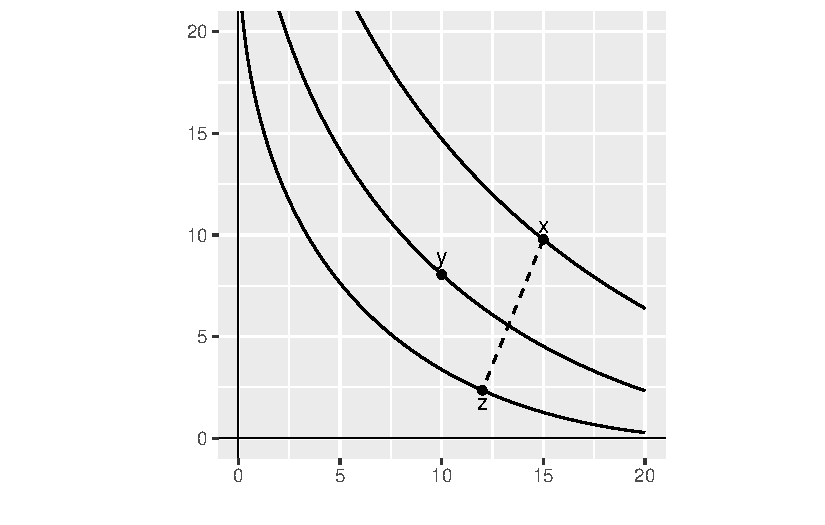
\includegraphics{risk-and-uncertainty/axioms-for-expected-utility-theory_files/figure-pdf/unnamed-chunk-1-1.pdf}

Note: If you read the literature about expected utility, you may come
across an axiom called the Archimedean property. Only one of continuity
or the Archimedean property need be assumed. I will not cover the
Archimedean property in this book.

\hypertarget{example-of-discontinuous-preferences}{%
\subsection{Example of discontinuous
preferences}\label{example-of-discontinuous-preferences}}

Lexiographic preferences occur where an agent prefers any amount of a
good \(x\) to any amount of another good \(y\). If choosing between
bundles of goods, the agent will choose the bundle with the most \(x\),
regardless of the amount of \(y\). They will only consider the amount of
\(y\) if the amount of \(x\) in two bundles is identical.

Consider an agent with lexiographic preferences who is offered the
following combinations of \(x\) and \(y\).

A. (1, 1)

B. (1, 2)

C. (1.1, 1)

Their preference ranking will be: \(C\succ B \succ A\).

This function is not continuous as there is a ``jump'' whenever there is
an increase in \(x\), even if \(y\) is large. Add an infinitesimal
amount \(\epsilon\) of \(x\) to bundle \(A\) and the preference relation
between bundle \(A\) and bundle \(B\) flips.

These three bundles \(A\), \(B\) and \(C\) are represented graphically
below.

First, let's consider these preferences in terms of Definition 1. Around
\(A\) I have drawn a circle of radius \(\epsilon\) (the neighbourhood).
No matter how small I draw this circle (no matter how small
\(\epsilon\)), any bundle within the circle that lies to the right of
\(A\) (that is, contains \(x>1\)) is preferred to bundle \(B\). There is
a jump in preferences to the right of A.

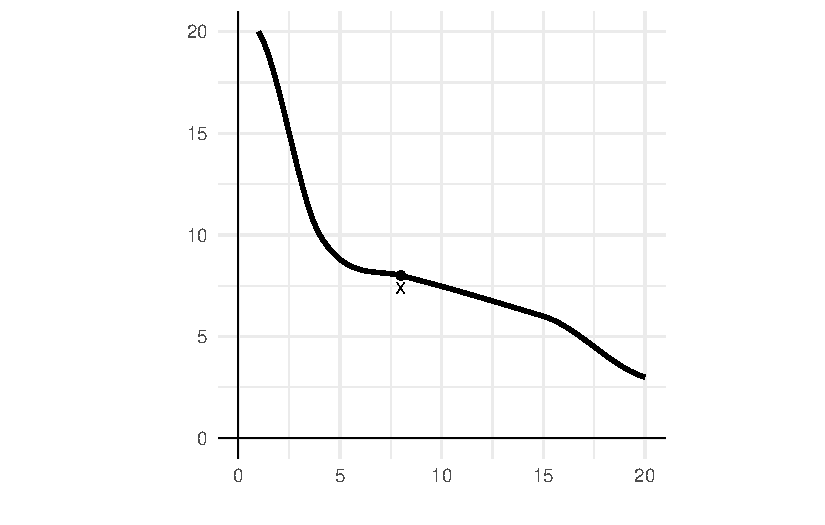
\includegraphics{risk-and-uncertainty/axioms-for-expected-utility-theory_files/figure-pdf/unnamed-chunk-2-1.pdf}

To consider this in terms of the second formal definition, there is no
\(p\) for which:

\[pA+(1-p)C \sim B\]

When \(p=1\), \(B \succ A\). For any \(p<1\), \(pA+(1-p)C \succ B\) as
any non-zero share of \(C\) makes the combination of \(A\) and \(C\)
preferred.

One interesting feature of lexiographic preferences is that you cannot
draw indifference curves on this figure. If a bundle differs from
another, it must be strictly preferred to the other as no amount of
\(y\) can make up for any amount of \(x\).

\hypertarget{sec-independence}{%
\section{Independence of irrelevant
alternatives}\label{sec-independence}}

Under independence of irrelevant alternatives, a person who mixes two
gambles with an irrelevant third gamble will maintain the same order of
preference between those two original gambles as when the two are
presented independently of the third.

Formally, if:

\begin{itemize}
\tightlist
\item
  \(x\) and \(y\) are lotteries with \(x\succcurlyeq y\) and
\item
  \(p\) is the probability that a third option \(z\) is present, then:
\end{itemize}

\[pz+(1-p)x\succcurlyeq pz+(1-p)y\]

The third choice, \(z\), is irrelevant. The order of preference for
\(x\) before \(y\) holds. It is independent of the presence of \(z\).

\hypertarget{example-of-independence-of-irrelevant-alternatives}{%
\subsection{Example of independence of irrelevant
alternatives}\label{example-of-independence-of-irrelevant-alternatives}}

Suppose \(x\) is an orange and \(y\) is an apple. I strictly prefer an
orange to an apple.

Suppose there is not a third possibility \(z\) of receiving no fruit.
Under the independence of irrelevant alternatives, if I prefer oranges
to apples, I will prefer a gamble with a 50\% chance of getting an
orange and 50\% chance of receiving nothing to a gamble with a 50\%
chance of getting an apple and a 50\% chance of receiving nothing.

That is:

\[\text{orange}\succ \text{apple}  \Longrightarrow 50\% \text{ chance of orange}\succ 50\% \text{ chance of apple}\]

\hypertarget{auxilliary-axioms}{%
\section{Auxilliary axioms}\label{auxilliary-axioms}}

Beyond completeness, transitivity, continuity and independence,
economists often adopt other axioms. These are not required for expected
utility theory, but make analysis more practicable.

These include:

\begin{itemize}
\item
  Utility is calculated over total wealth.
\item
  Non-satiation: No matter what you have, there is always another
  (nearby) bundle that you would rather have.
\item
  Monotonicity: Preferences are monotone if more of any good in the
  bundle makes the agent strictly better off. Non-satiation is implied
  by monotonicity, but not the other way around. Monotonicity implies
  downward sloping indifference curves.
\item
  Convexity: Convexity means that people have a preference for variety
  or combination (indifference curves bulge toward the origin).
\item
  Diminishing marginal utility: Each successive additional unit of
  consumption delivers a smaller (diminishing) amount of utility than
  the last.
\end{itemize}

I provide further detail on convexity and diminishing marginal utility
below.

\hypertarget{convexity}{%
\subsection{Convexity}\label{convexity}}

Convexity means that people have a preference for variety or combination
(indifference curves bulge toward the origin). Averages are better than
extremes.

In many contexts this makes sense. For example, suppose an agent is
indifferent between two beers and two meat pies. Under this assumption,
any mix of the two (e.g.~a beer and a pie) will be at least as preferred
as the two beers or two pies.

Formally, a preference relation is convex if, for any
\(x\succcurlyeq y\) and for every \(\theta\in[0,1]\):

\[\theta x+(1-\theta)y\succcurlyeq y\]

Strict convexity is where, for any \(x\sim y\), \(x\neq y\) and for
every \(\theta\in[0,1]\):

\[\theta x+(1-\theta)y\succcurlyeq y\]

\[\theta x+(1-\theta)y\succcurlyeq x\]

For two equivalent goods or bundles, a weighted average of the two
bundles is better than each of those bundles.

\hypertarget{diminishing-marginal-utility}{%
\subsection{Diminishing marginal
utility}\label{diminishing-marginal-utility}}

Marginal utility is how much utility you get or lose from an incremental
decrease or increase in consumption. Under diminishing marginal utility,
each successive additional unit of consumption delivers a smaller
(diminishing) amount of utility than the last.

Diminishing marginal utility leads to risk averse preferences.

Diminishing marginal utility is related to the axiom of convexity.
Diminishing marginal utility will lead to convex indifference curves.
However, the reverse relationship does not always hold.

\hypertarget{expected-utility-theory}{%
\chapter{Expected Utility Theory}\label{expected-utility-theory}}

\hypertarget{maximising-expected-utility}{%
\section{Maximising expected
utility}\label{maximising-expected-utility}}

People do not seek to maximize expected value, but instead maximize
expected utility.

Under expected utility theory, people choose between risky prospects
(another word for lottery or gamble common in the literature) by
comparing expected utility values. The agent maximises expected utility,
\(E[U(x)]\):

\begin{align*}
E[U(x)]&=p_1U(x_1)+p_2U(x_2)+ ... +p_nU(x_n) \\[6pt]
&=\sum_{i=1}^n p_iU(x_i)
\end{align*}

\(p_i\) is the probability of outcome \(x_i\).

\(U(x_i)\) is the utility of outcome \(x_i\)

Under Expected Utility Theory, risky options are evaluated in 3 steps:

\begin{enumerate}
\def\labelenumi{\arabic{enumi}.}
\item
  Define utility over final outcomes \(x_1, ..., x_n\)
\item
  Weight utility of each outcome \(U(x_i)\) by the probability of
  outcome \(p_i\)
\item
  Add the weighted utilities
\end{enumerate}

There is an important note to make here regarding outcomes
\(x_1, ..., x_n\). Typically, these outcomes are not just the payoffs
from the gamble, but rather the agent's final position. If the agent has
wealth of \$100 and is offered a coin flip to win or lose \$10, the
outcomes are typically taken to be \$90 and \$110. Their decision
depends on their current wealth. As a result, expected utility is often
represented as:

\begin{align*}
E[U(W+x)]&=p_1U(W+x_1)+p_2U(W+x_2)+ ... +p_nU(W+x_n) \\[6pt]
&=\sum_{i=1}^n p_iU(W+x_i)
\end{align*}

\hypertarget{attitudes-toward-risk}{%
\section{Attitudes toward risk}\label{attitudes-toward-risk}}

Expected utility theory captures an individual's risk preference by
means of their utility function.

If a person prefers a sure amount over a gamble with comparable expected
value, they are risk averse.

If a person prefers the gamble over the sure amount, they are risk
seeking.

If a person is indifferent, they are risk neutral.

The certainty equivalent (CE) of a gamble X is the the amount of money
such that you are indifferent between taking the gamble and taking the
money:

\[u(CE)=EU(X)\]

\hypertarget{risk-aversion}{%
\subsection{Risk aversion}\label{risk-aversion}}

For a risk averse person, the certainty equivalent is less than the
expected value of the gamble.

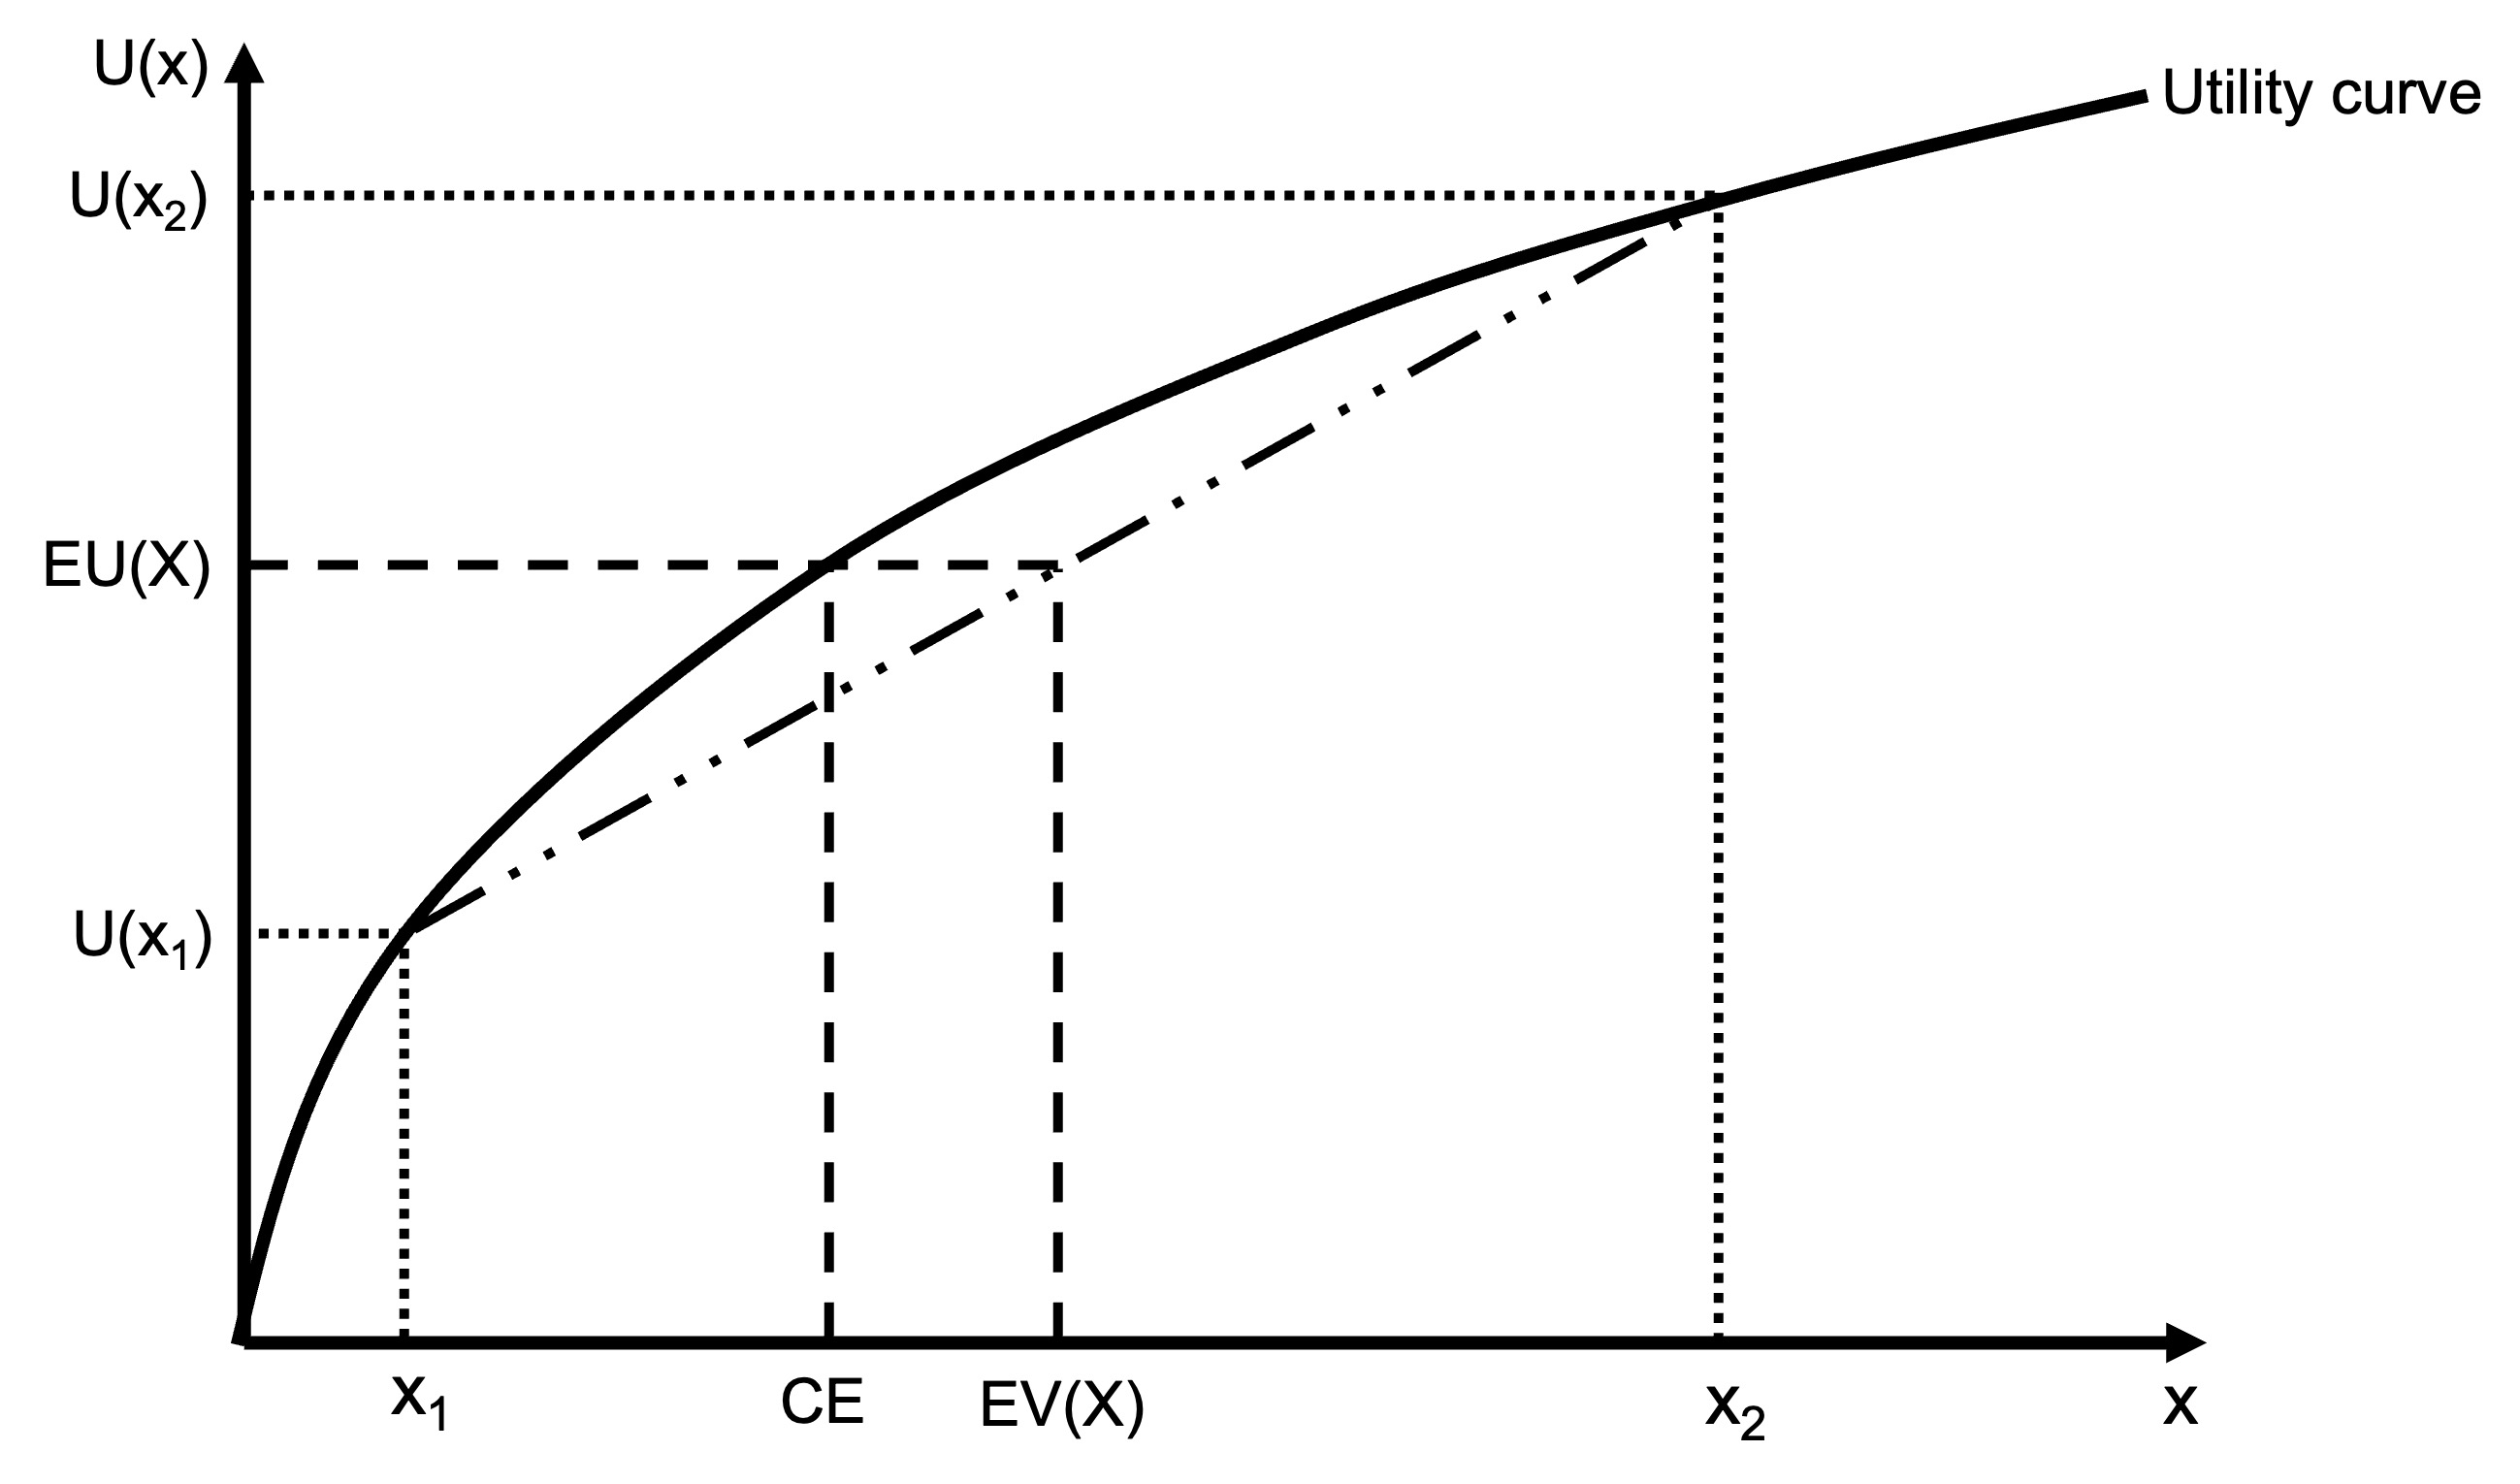
\includegraphics{risk-and-uncertainty/img/risk-averse.jpg}

\hypertarget{risk-neutrality}{%
\subsection{Risk neutrality}\label{risk-neutrality}}

For a risk averse person, the certainty equivalent is equal to the
expected value of the gamble. A risk neutral person is an expected value
maximiser.

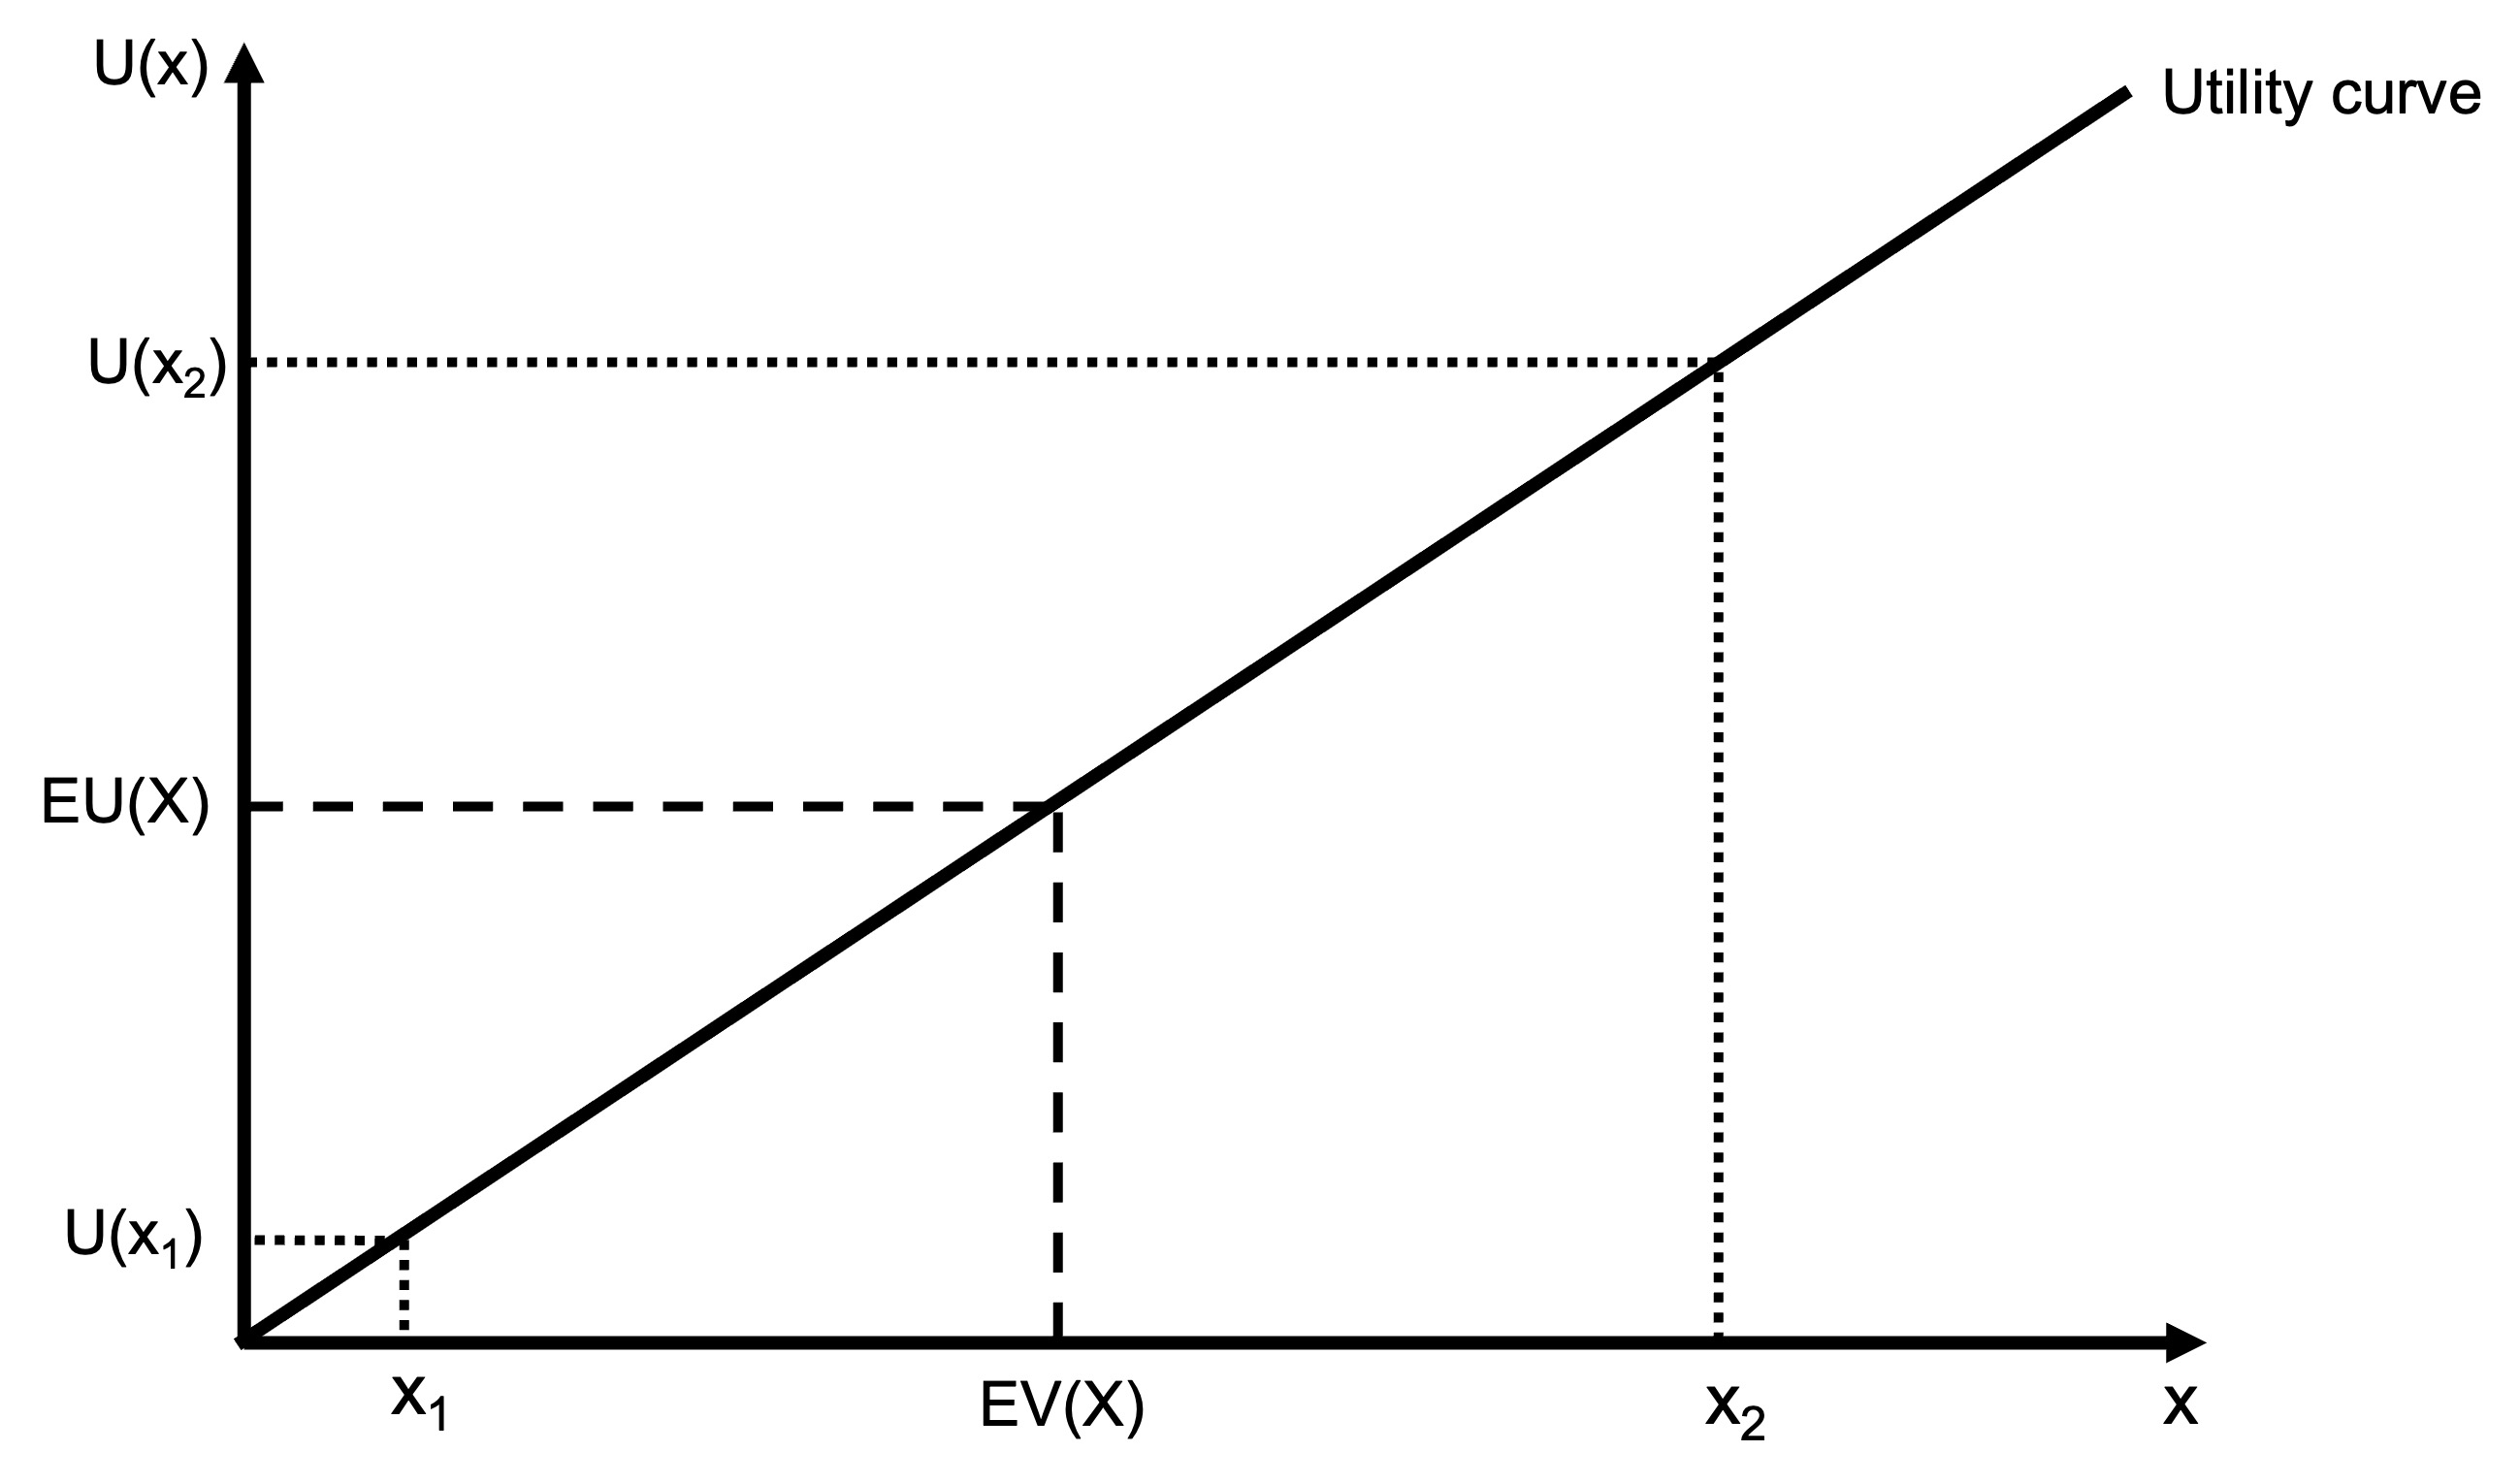
\includegraphics{risk-and-uncertainty/img/risk-neutral.jpg}

\hypertarget{risk-seeking}{%
\subsection{Risk seeking}\label{risk-seeking}}

For a risk seeking person, the certainty equivalent is more than the
expected value of the gamble. The gamble has value in and of itself.

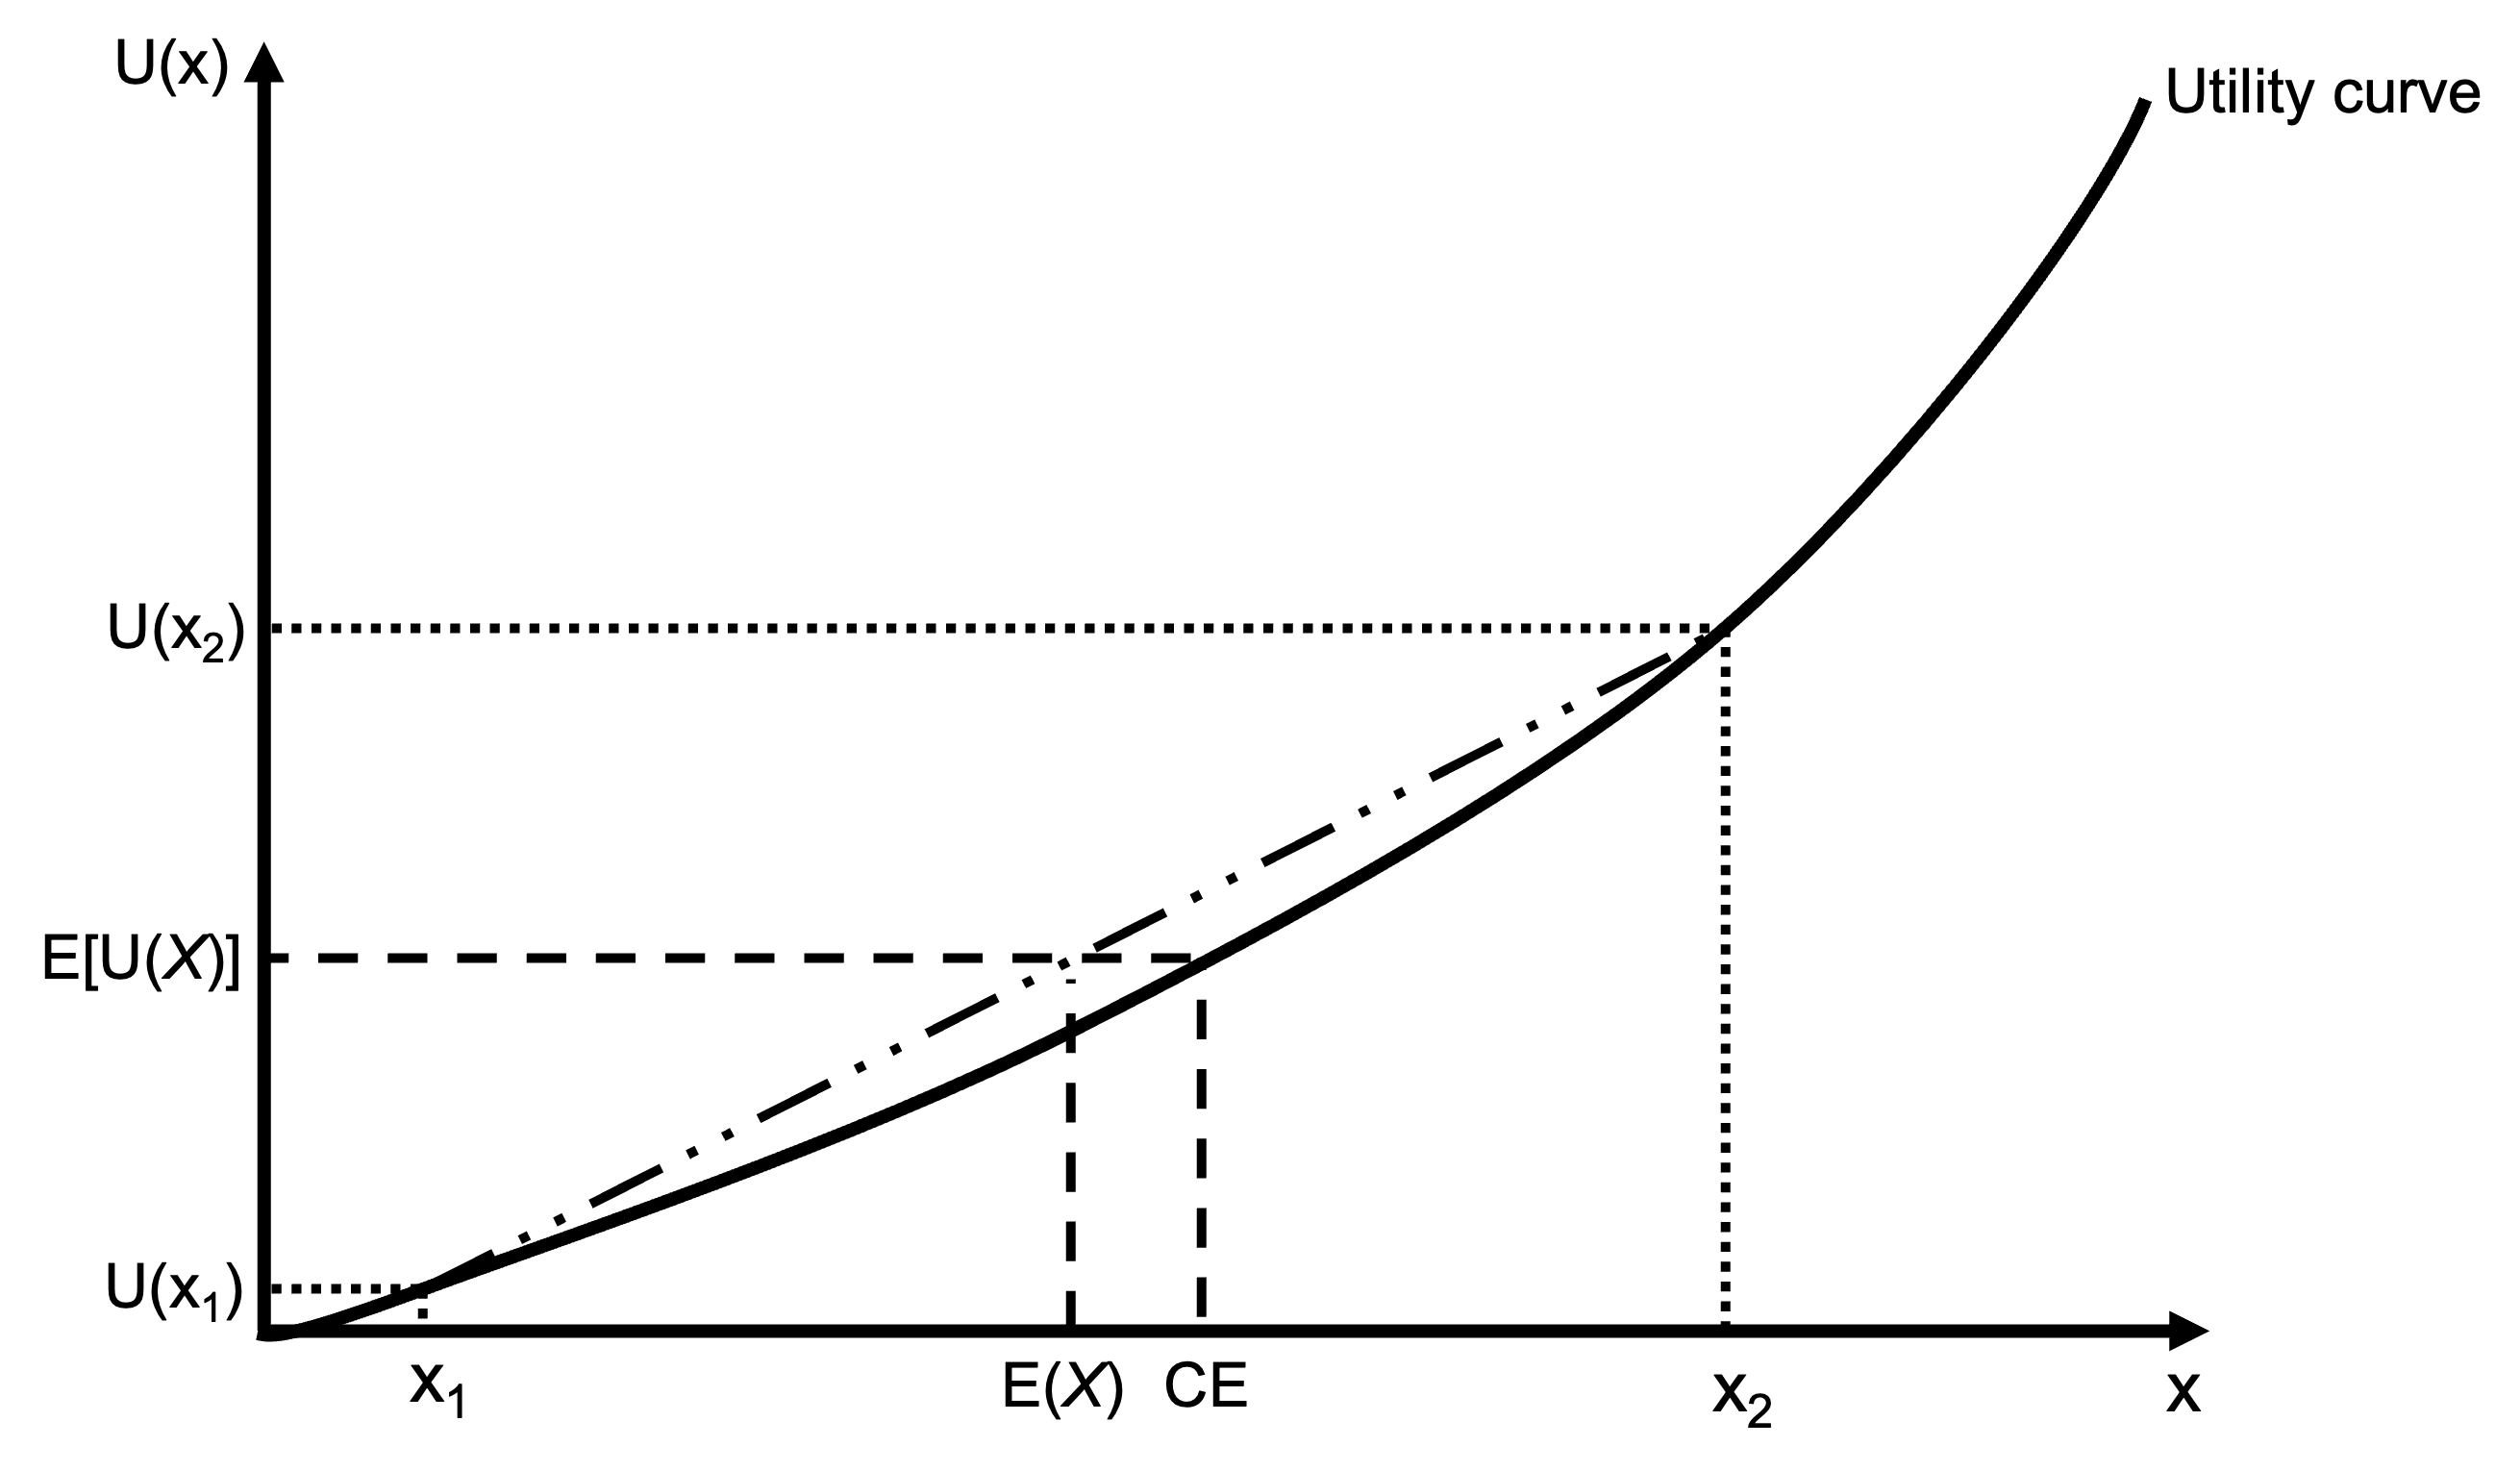
\includegraphics{risk-and-uncertainty/img/risk-seeking.png}

\hypertarget{subjective-expected-utility}{%
\chapter{Subjective Expected
Utility}\label{subjective-expected-utility}}

Subjective expected utility theory is used in situations of uncertainty,
where the probabilities are not known. People maximize expected utility
using a subjective estimate of probability.

The agent maximises subjective expected utility, \(E[U(x)]\):

\begin{align*}
E[U(x)]&=\pi(x_1)U(x_1)+\pi(x_2)U(x_2)+...+\pi(x_n)U(x_n)\\[6pt]
&=\sum_{i=1}^n \pi(x_i)U(x_i)
\end{align*}

where \(\pi(x_i)\) is the subjective probability of \(x_i\).

People have different beliefs about the probabilities of different
outcomes, but these typically come from a ``sound'' foundation such as
Bayesian probability theory. Decision makers are Bayesian, in that,
given the evidence, they have beliefs which are consistent with Bayes'
rule.

In Subjective Expected Utility Theory, uncertain options are evaluated
in 4 steps:

\begin{enumerate}
\def\labelenumi{\arabic{enumi}.}
\item
  Define utility over final outcomes \(x_1,...,x_n\).
\item
  Define subjective probability \(\pi(x_i)\) over final outcomes
  \(x_1,...,x_n\).
\item
  Weight utility of each outcome \(U(x_i)\) by the subjective
  probability \(\pi(x_i)\).
\item
  Add the weighted utilities.
\end{enumerate}

\hypertarget{expected-utility-examples}{%
\chapter{Expected utility examples}\label{expected-utility-examples}}

\hypertarget{example-1-1}{%
\section{Example 1}\label{example-1-1}}

Suppose your utility function is \(U(x)=ln(x)\).

You have a 50\% chance of winning \$10 and a 50\% chance of losing \$10.
Assume your starting wealth is \$20.

What is the expected value of this game?

\begin{align*}
E[x]&=\sum_{i=1}^n p_ix_i \\[6pt]
&=0.5*10+0.5*(-10) \\[6pt]
&=0
\end{align*}

The expected value of the game is \$0.

What is the expected utility of this game?

\begin{align*}
E[U(W+x)]&=\sum_{i=1}^n p_iU(x_i+W) \\[6pt]
&=0.5U(20-10)+0.5U(20+10) \\[6pt]
&=0.5ln(10)+0.5ln(30) \\[6pt]
&=2.85
\end{align*}

What does an expected utility of 2.85 mean? To make it tangible, we can
ask what wealth would give that utility.

\[U(W)=ln(W)=2.85\]

\[W=e^{2.85}=\$17.30\]

This gamble with expected value of zero reduces utility by an amount
equivalent to \$2.70.

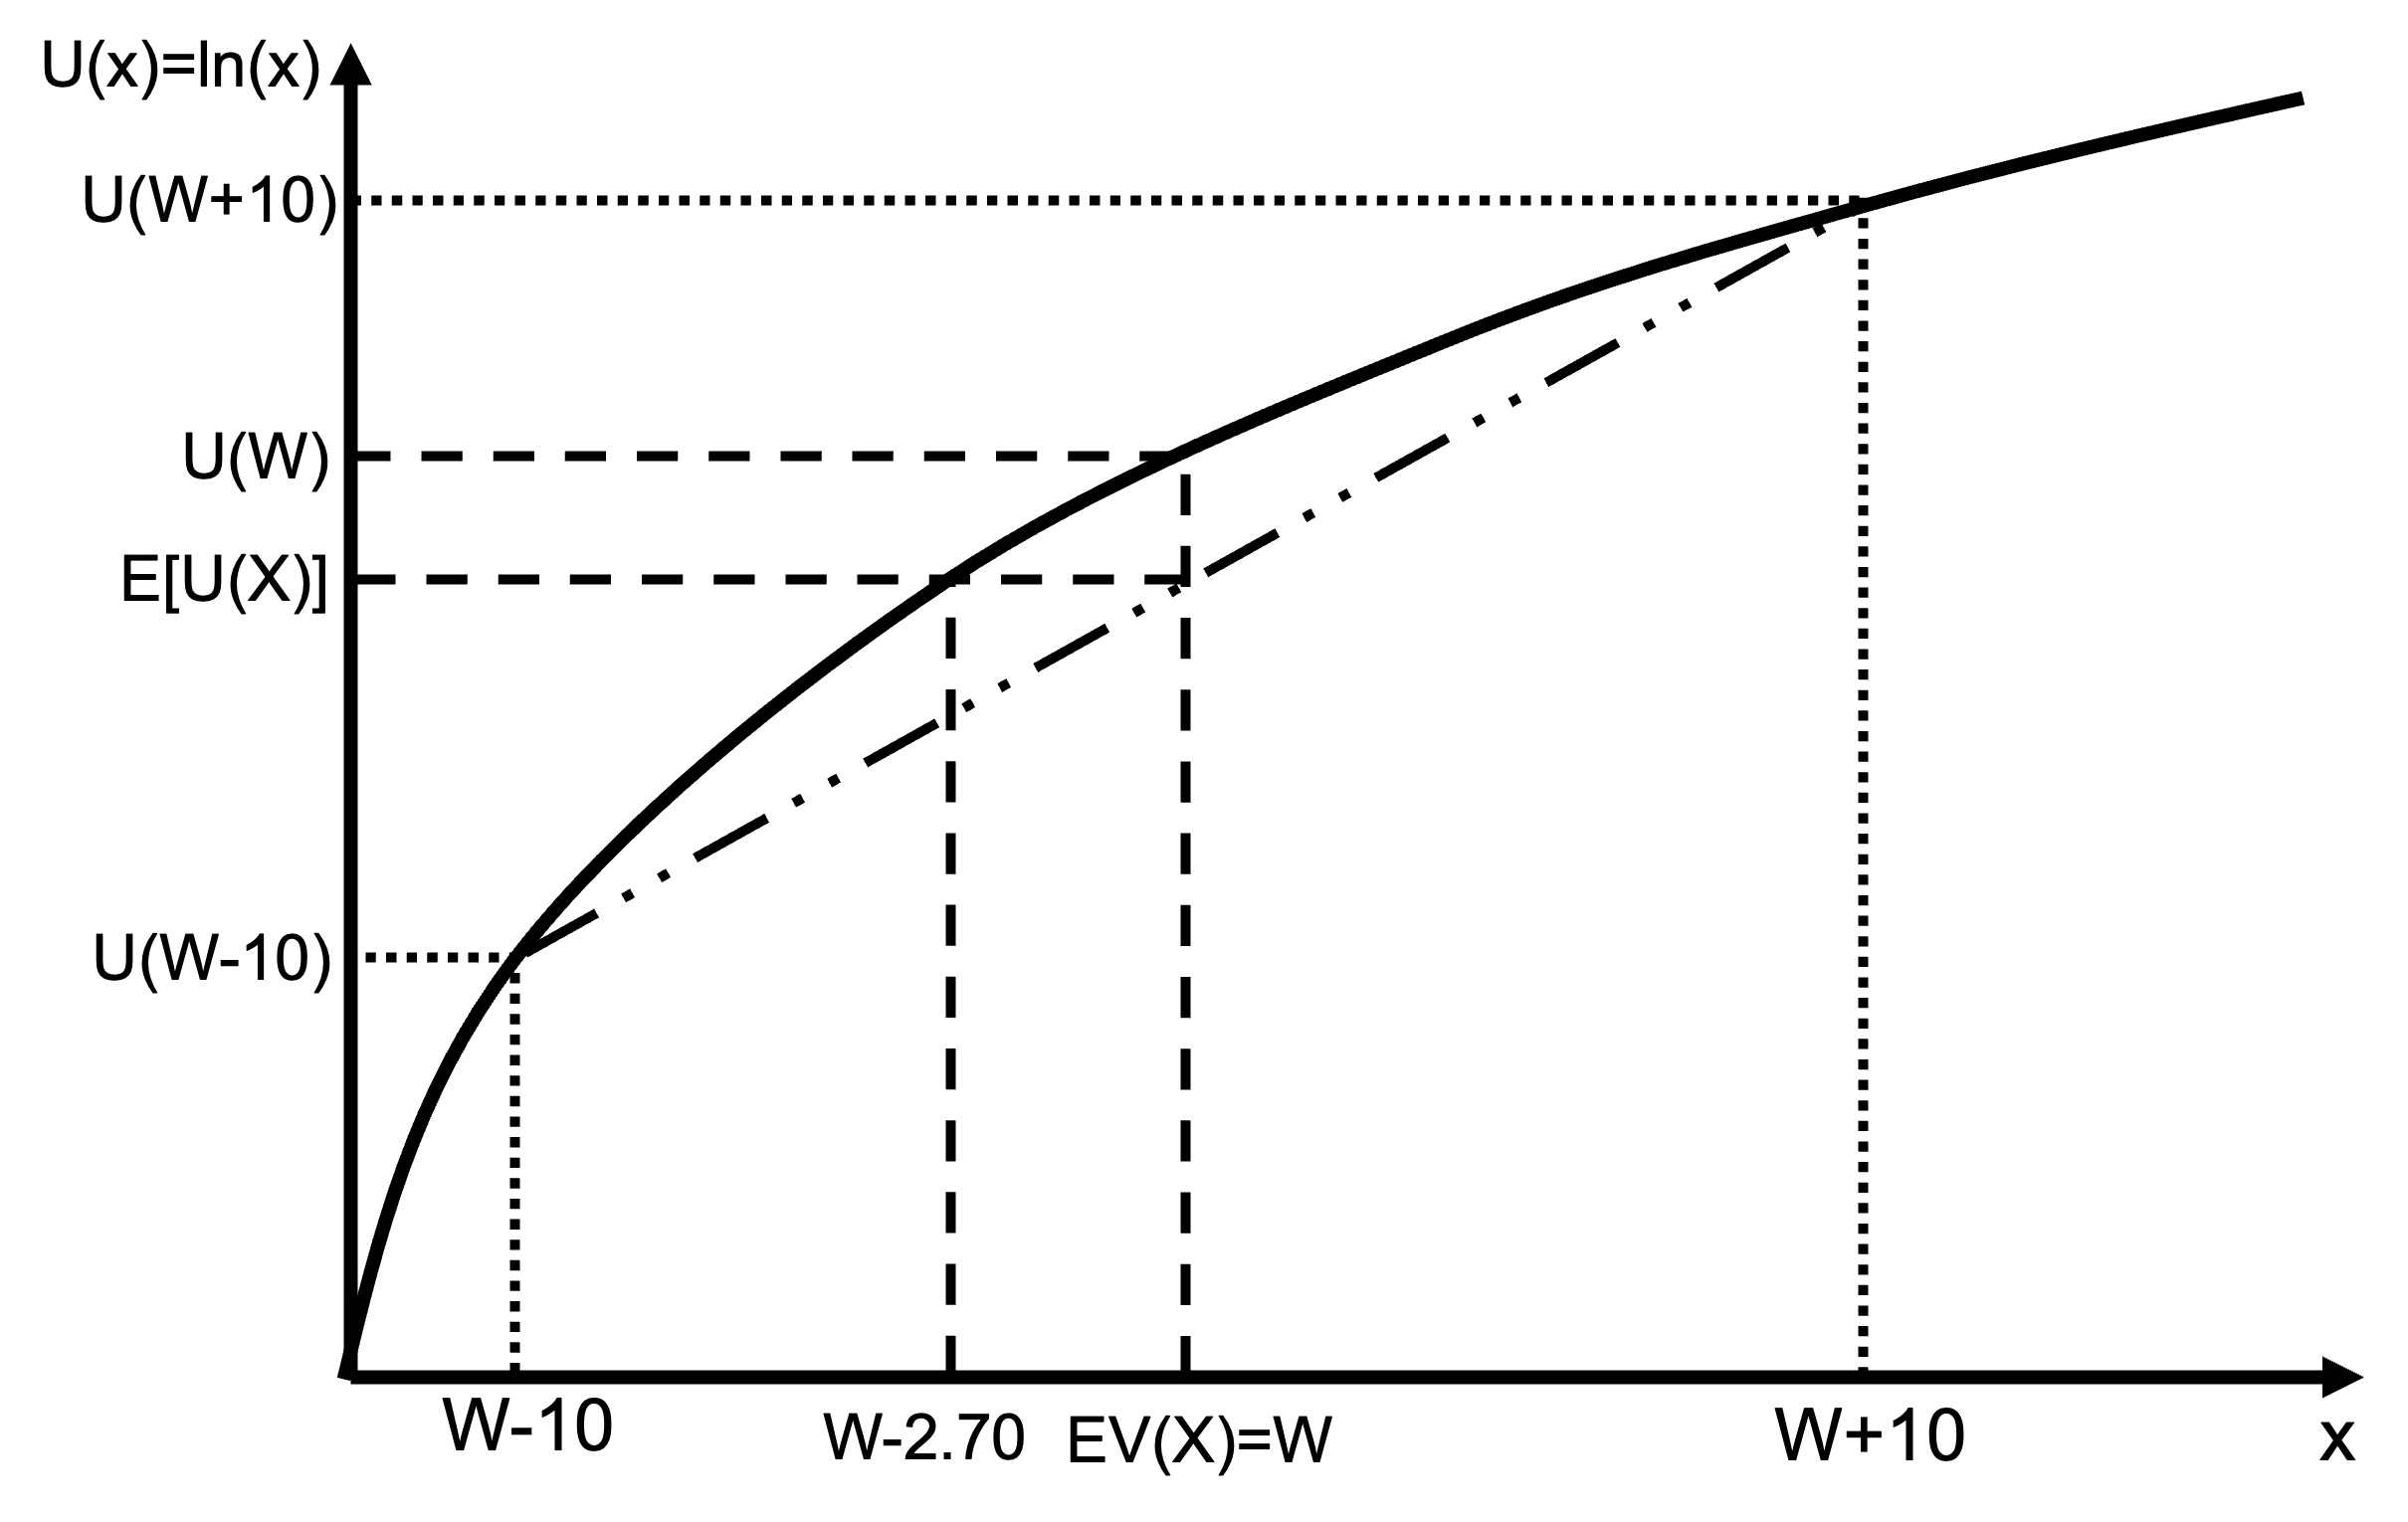
\includegraphics{risk-and-uncertainty/img/expected-utility-example.jpg}

We could also say that the certainty equivalent of this gamble is final
wealth of \$17.30, a loss of \$2.70.

\hypertarget{example-2-1}{%
\section{Example 2}\label{example-2-1}}

Suppose your utility function is \(\small U(x)=ln(x)\).

You have an 80\% chance of winning \$10 and a 50\% chance of losing
\$10. Assume your starting wealth is \$20.

What is the expected value and the expected utility of this game?

\begin{align*}
E[x]&=\sum_{i=1}^n p_ix_i \\[6pt]
&=0.8*10+0.2*(-10) \\[6pt]
&=\$6
\end{align*}

The expected value of the game is \$6.

\begin{align*}
E[U(W+x)]&=\sum_{i=1}^n p_iU(x_i+W) \\[6pt]
&=0.8U(20+10)+0.2U(20-10) \\[6pt]
&=0.8ln(30)+0.2ln(10) \\[6pt]
&=3.18
\end{align*}

What does an expected utility of 3.18 mean? To make it tangible, we can
ask what wealth would give that utility.

\[U(W)=ln(W)=3.18\]

\[W=e^{3.18}=\$24.08\]

This gamble with expected value of \$6 increases utility by an amount
equivalent to \$4.08.

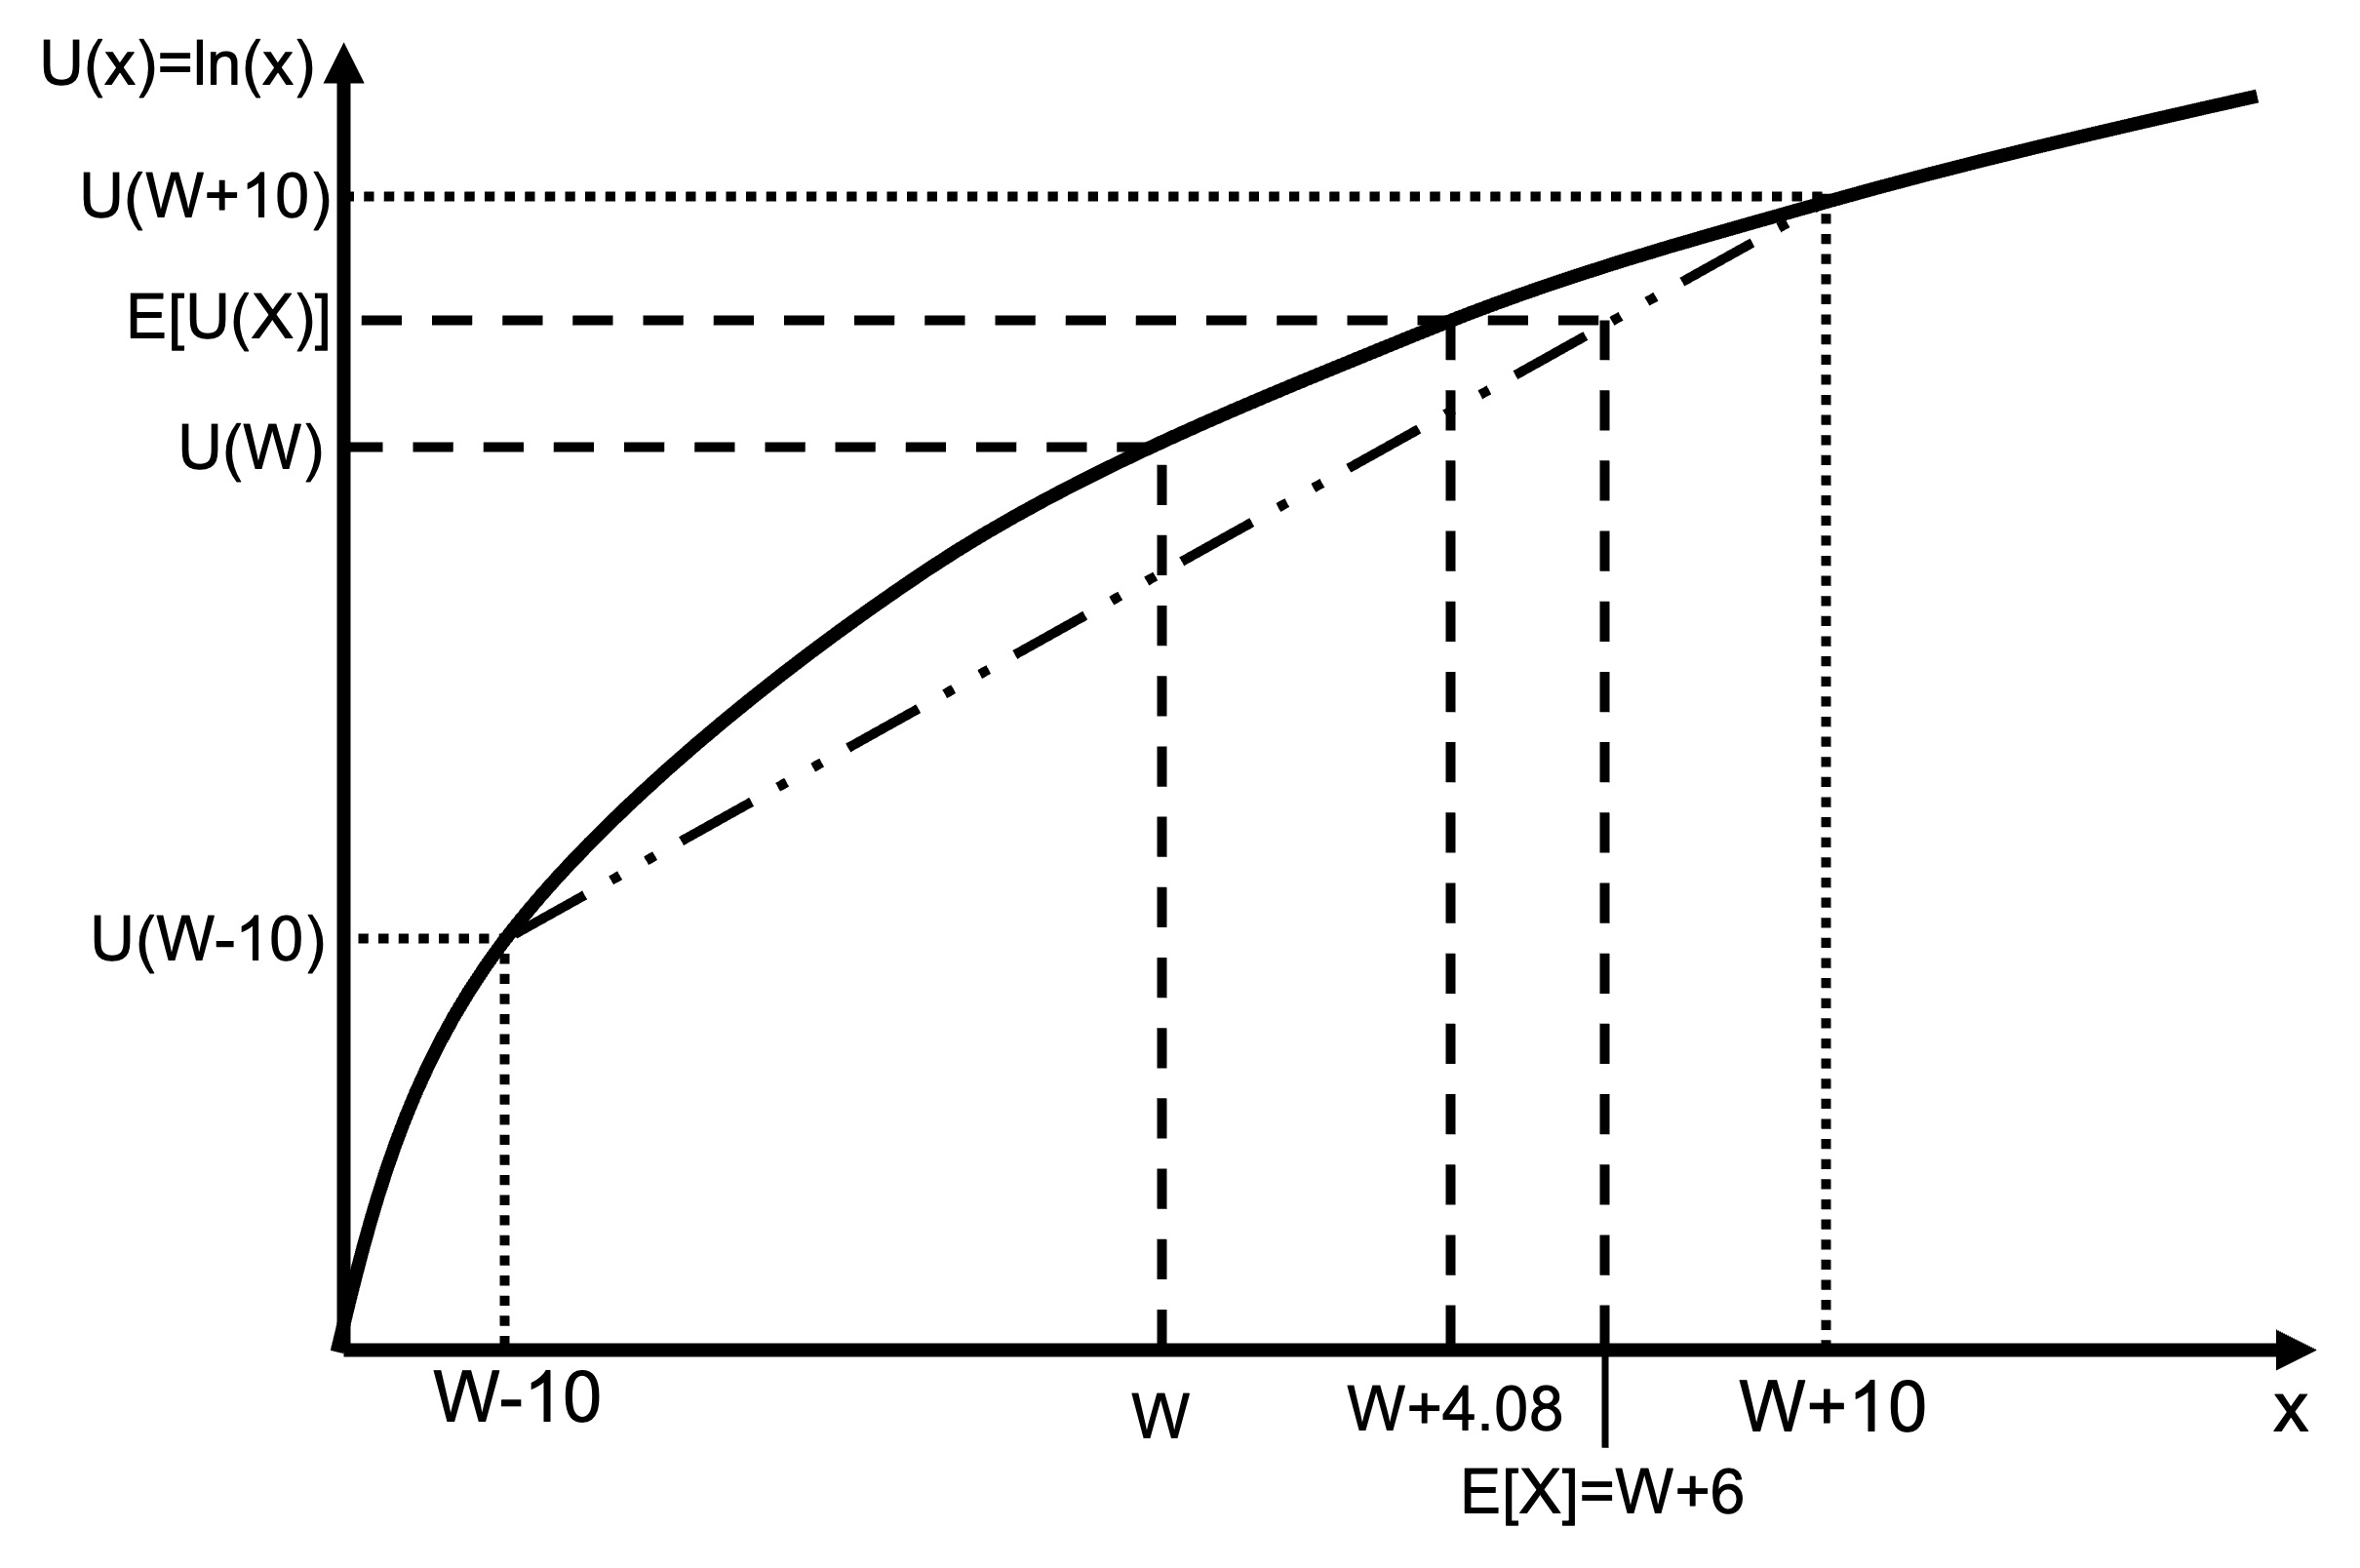
\includegraphics{risk-and-uncertainty/img/expected-utility-example-2.jpg}

\hypertarget{example-3}{%
\section{Example 3}\label{example-3}}

Suppose your utility function is \(U(x)=ln(x)\).

You have a 50\% chance of increasing your wealth by 50\% and a 50\%
chance of decreasing your wealth by 40\%.

What is the expected value and the expected utility of this games?

\begin{align*}
E[U(X)]&=\sum_{i=1}^n p_iU(X_i) \\[6pt]
&=0.5U(0.6W)+0.5U(1.5W) \\[6pt]
&=0.5ln(0.6)+0.5*ln(W)+0.5ln(1.5)+0.5*ln(W) \\[6pt]
&=-0.255+0.203+ln(W) \\[6pt]
&=−0.053+ln(W)
\end{align*}

Here we have a gamble with a positive expected value, 5\% of your
wealth, but lower expected utility. Someone with log utility would
reject this bet.

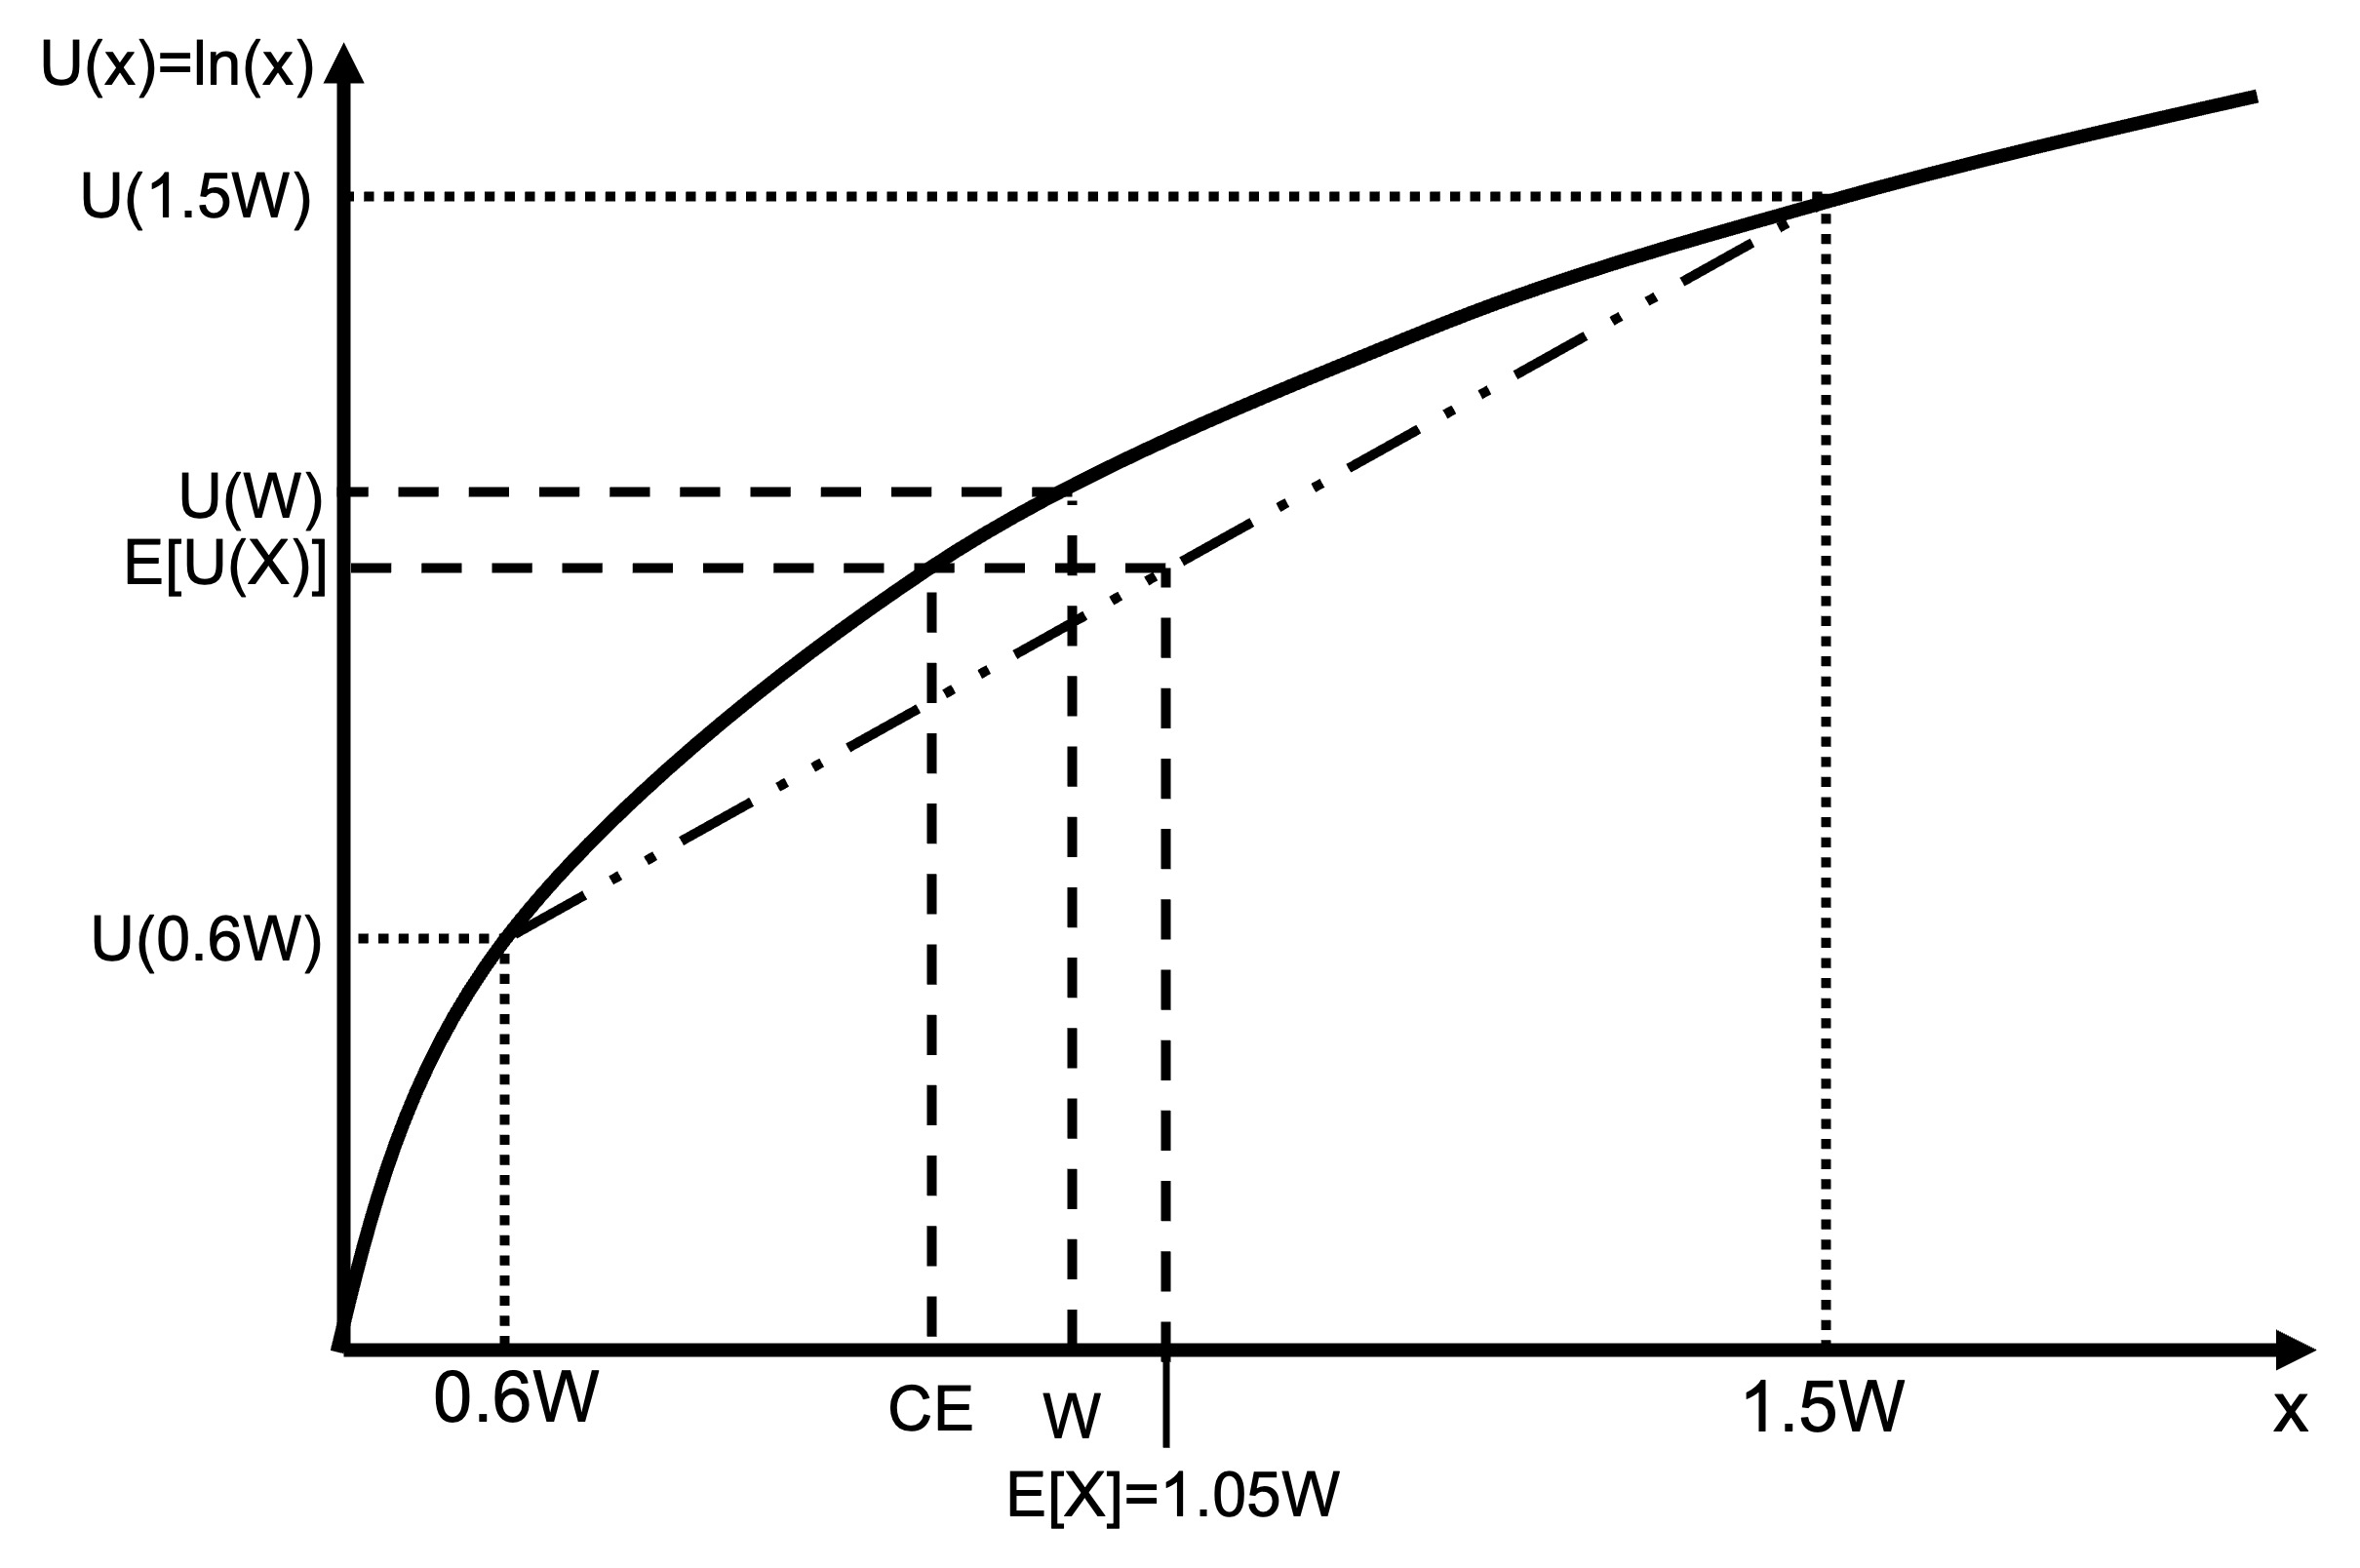
\includegraphics{risk-and-uncertainty/img/expected-utility-example-3.jpg}

\hypertarget{example-4-the-st.-petersburg-game}{%
\section{Example 4: The St.~Petersburg
game}\label{example-4-the-st.-petersburg-game}}

The St.~Petersburg game was invented by Swiss mathematician Nicolas
Bernoulli.

The game starts with a pot containing \$2. A dealer then flips a coin.
The pot doubles every time a head appears. The game ends and the player
win the pot as soon as tails appears.

\begin{itemize}
\tightlist
\item
  Tail on the first flip: \$2
\item
  Tail on the second flip: \$4
\item
  Tail on the third flip: \$8
\item
  Tail on the fourth flip: \$16
\end{itemize}

And so on.

The expected value of this game is equal to:

\begin{align*}
E[X]&=\underbrace{\frac{1}{2}*2}_\textrm{Tail first}+\underbrace{(\frac{1}{2}*\frac{1}{2})*4}_\textrm{Tail second}+\underbrace{(\frac{1}{2}*\frac{1}{2}*\frac{1}{2})*8}_\textrm{Tail third} \\[24pt]
&\qquad +\underbrace{(\frac{1}{2}*\frac{1}{2}*\frac{1}{2}*\frac{1}{2})*16}_\textrm{Tail fourth}+... \\[24pt]
&=1+1+1+1+... \\
&=\sum_{k=1}^\infty 1 \\
&=\infty
\end{align*}

The \(\sum\) operator means ``sum for \(k=1\) to \(k=\infty\)''.

The expected utility of this game is equal to:

\begin{align*}
E[U(X)]&=\underbrace{\frac{1}{2}*U(W+2)}_\textrm{Tail first}+\underbrace{(\frac{1}{2}*\frac{1}{2})*U(W+4)}_\textrm{Tail second} \\[24pt] 
&\qquad +\underbrace{(\frac{1}{2}*\frac{1}{2}*\frac{1}{2})*U(W+8)}_\textrm{Tail third}
+\underbrace{(\frac{1}{2}*\frac{1}{2}*\frac{1}{2}*\frac{1}{2})*U(W+16)}_\textrm{Tail fourth}+... \\[24pt]
&=\frac{1}{2}U(W+2)+\frac{1}{4}U(W+4)+\frac{1}{8}U(W+8)+\frac{1}{16}U(W+16)+...  \\[12pt]
&=\sum_{k=1}^{k=\infty}\frac{1}{2^k}U(W+2^k)
\end{align*}

What is the maximum \$\(c\) a risk neutral player with \(U(x)=x\) would
be willing to pay to play the game? One strategy to determine \$\(c\) is
to ask at what \$\(c\) the player would be indifferent between accepting
and rejecting a chance to play. That is the maximum \$\(c\) that they
would be willing to pay. They will be indifferent when
\(U(W)=E[U(X-c)]\).

\begin{align*}
U(W)&=E[U(X-c)] \\[6pt]
U(W)&=\sum_{k=1}^{k=\infty}\frac{1}{2^k}(U(W+\$2^k-c) \\[6pt]
W&=\sum_{k=1}^{k=\infty}\frac{1}{2^k}(W+2^k-c) \\[6pt]
W&=W-c+\sum_{k=1}^{k=\infty}1 \qquad \bigg(\text{as }\sum_{k=1}^{k=\infty}\frac{1}{2^k}=1\bigg) \\[12pt]
c&=\infty
\end{align*}

A risk-neutral player would pay any amount \$\(c\) to play.

What is the maximum \(\$c\) a risk averse player with \(U(x)=ln(x)\)
player would be willing to pay to play the game? How does their wealth
affect their willingness to pay?

Again we will determine at what \$\(c\) the player is indifferent
between accepting and rejecting a chance to play, which occurs when
\(U(W)=E[U(X-c)]\).

\begin{align*}
U(W)&=E[U(X-c)] \\[6pt]
U(W)&=\sum_{k=1}^{k=\infty}\frac{1}{2^k}U(W+\$2^k-c) \\[6pt]
ln(W)&=\sum_{k=1}^{k=\infty}\frac{1}{2^k}ln(W+\$2^k-c)
\end{align*}

There is no closed form solution to this equation to enable us to
determine \(c\). It needs to be solved via numerical methods (such as
testing and iterating to a solution). Someone who has wealth of \$0.01
would be willing to pay up to \$2.01 (they would need to borrow).
Someone with wealth \$1000 would be willing to pay \$10.95, while a
person with wealth of \$1 million would be willing to pay \$20.87.

Note: we cannot solve for a person with no wealth as ln⁡(0) is undefined.

Another way to gain an intuition of what is happening to ask what is the
utility of a risk averse player whose only asset is the opportunity to
play this game.

\begin{align*}
E[U(X)]&=\sum_{k=1}^{k=\infty}\frac{1}{2^k}U(\$2^k) \\[12pt]
&=\sum_{k=1}^{k=\infty}\frac{1}{2^k}ln(2^k) \\[12pt]
&=\sum_{k=1}^{k=\infty}\frac{k}{2^k}ln(2) \\[12pt]
&=\frac{1}{2}ln(2)+\frac{2}{4}ln(2)+\frac{3}{8}ln(2)+\frac{4}{16}ln(2)+\frac{5}{32}ln(2)+... \\[12pt]
&=(\frac{1}{2}+\frac{1}{2}+\frac{3}{8}+\frac{1}{4}+\frac{5}{32}+...)ln(2) \\[12pt]
&=2ln(2)
\end{align*}

The change in utility from each flip rapidly converges as the series of
fractions sums to two. The expected utility from the game is equal to
the utility of \$4 \((U(W)=ln(W)=2ln(2);\space W=e^{2ln2}=4)\).

Why does willingness to pay increase with wealth?

With log utility, as wealth increases the slope of the log function
increasingly approximates a linear function (the second derivative
approaches zero). Hence, the gambler displays less risk averse (closer
to risk neutral) behaviour.

\hypertarget{anomalies-of-expected-utility-theory}{%
\chapter{Anomalies of expected utility
theory}\label{anomalies-of-expected-utility-theory}}

\hypertarget{sec-allais}{%
\section{The Allais Paradox}\label{sec-allais}}

\textbf{Choice 1}: Choose one of the following bets:

Bet A:

\begin{itemize}
\tightlist
\item
  \$2500 with probability: 33\%
\item
  \$2400 with probability: 66\%
\item
  \$0 with probability: 1\%
\end{itemize}

Bet B:

\begin{itemize}
\tightlist
\item
  \$2400 with probability: 100\%
\end{itemize}

\textbf{Choice 2}: Choose one of the following bets:

Bet C:

\begin{itemize}
\tightlist
\item
  \$2500 with probability: 33\%\\
\item
  \$0 with probability: 67\%
\end{itemize}

Bet D:

\begin{itemize}
\tightlist
\item
  \$2400 with probability: 34\%
\item
  \$0 with probability: 66\%
\end{itemize}

When Kahneman and Tversky (1979) ran this experiment 82\% of
participants chose option B and 83\% of participants chose option C.

According to Expected Utility Theory, if an agent selects B:

\[
U(2400)>0.33U(2500)+0.66U(2400)+0.01U(0)
\]

\[
0.34U(2400)>0.33U(2500)+0.01U(0)
\]

According to Expected Utility Theory, if an agent selects C:

\[
0.33U(2500)+0.67U(0)> 0.34U(2400)+ 0.66U(0)
\]

\[
0.33U(2500)+0.01U(0)> 0.34U(2400)
\]

This is a contradiction. Under expected utility theory, if an agent
chooses A it should choose C. And if the agent chooses B it should
choose D. This phenomena is called the Allais Paradox after Maurice
Allais (1953), who first identified it.

Why does this occur? What axiom is being breached?

Here is another representation of the choices.

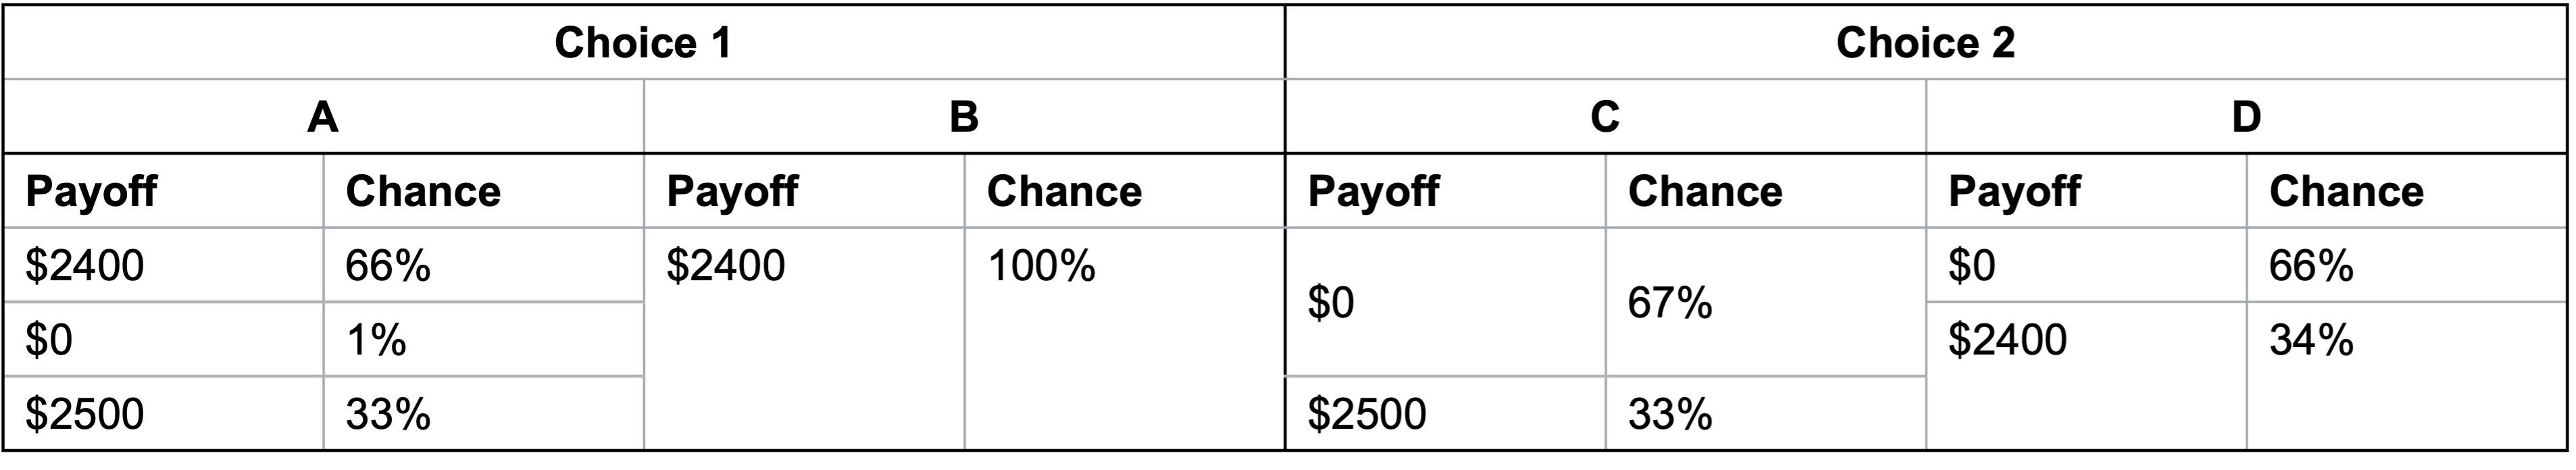
\includegraphics{risk-and-uncertainty/img/allais-paradox-1.jpg}

This second tabular representation is equivalent. I have split the
outcomes in options B and C.

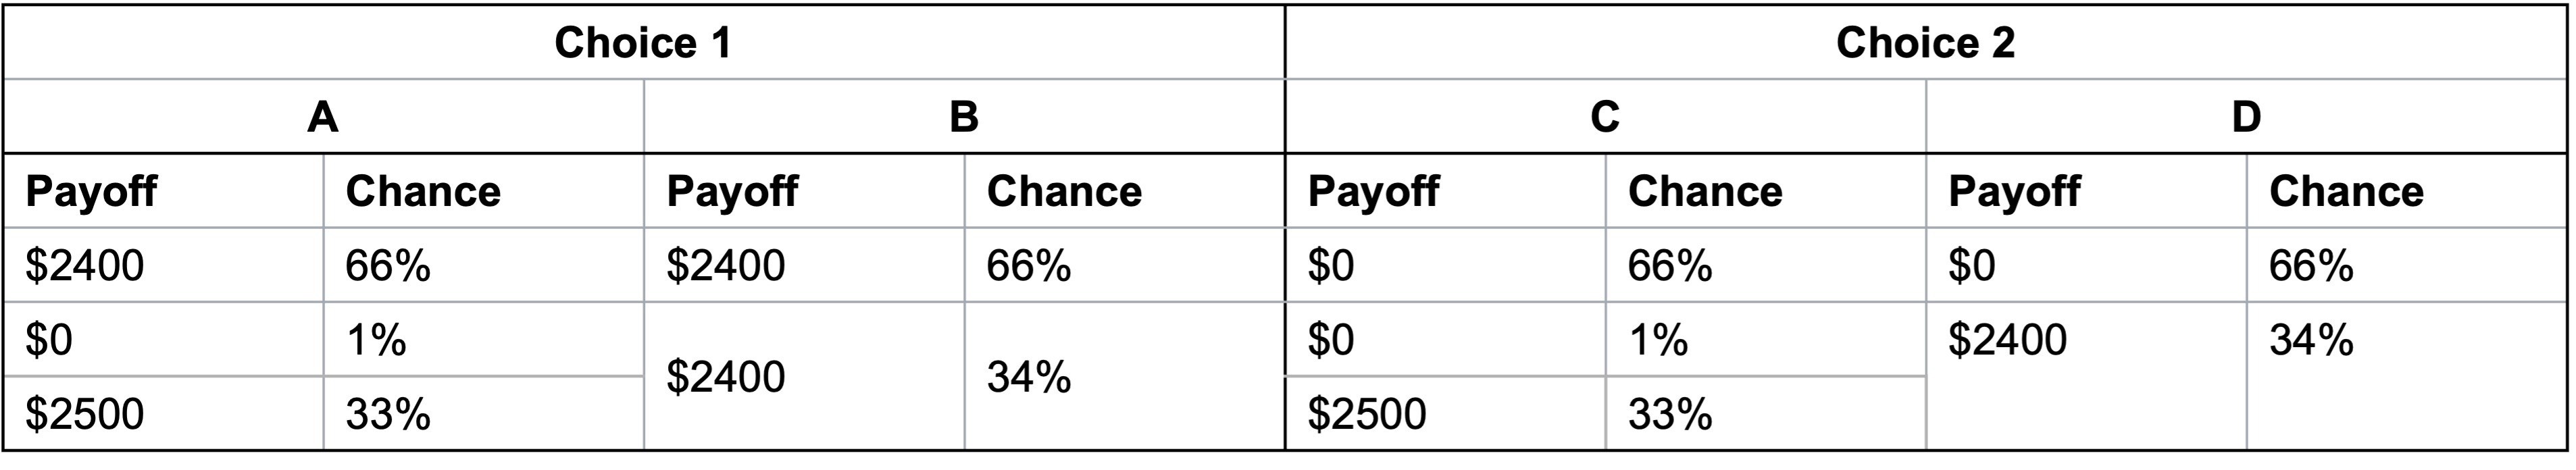
\includegraphics{risk-and-uncertainty/img/allais-paradox-2.jpg}

You can see that the bets contained in the bottom two rows are the same.
For choice 1, they are paired with a 66\% chance of winning \$2400, and
for choice 2 a 66\% chance of winning \$0.

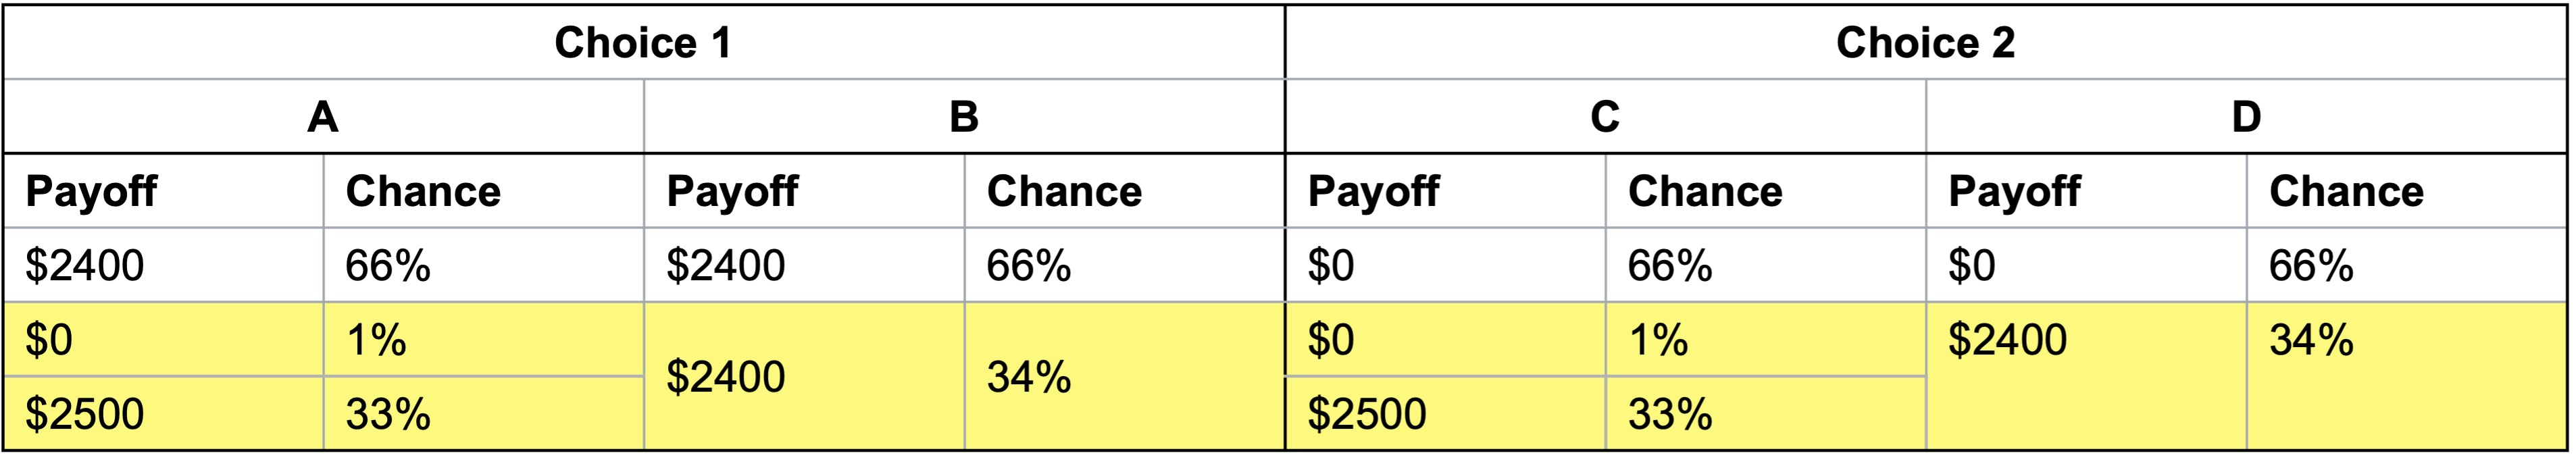
\includegraphics{risk-and-uncertainty/img/allais-paradox-3.jpg}

Preferring B to A and C to D is a violation of the axiom of the
\href{@sec-independence}{independence of irrelevant alternatives}: Under
that axiom, two gambles mixed with an irrelevant third gamble will
maintain the same order of preference as when the two are presented
independently of the third gamble.

Recall that the formal definition for the independence of irrelevant
alternatives axiom is that if:

\begin{itemize}
\tightlist
\item
  \(x\) and \(y\) are lotteries with \(x\succcurlyeq y\) and
\item
  \(p\) is the probability that a third option \(z\) is present, then:
\end{itemize}

\[pz+(1-p)x\succcurlyeq pz+(1-p)y\]

For each of the choices in our lottery:

\begin{itemize}
\item
  \(p=66%
  \)
\item
  \(x\) is a 100\% chance of \$2400
\item
  \(y\) is a 0.01/(1−0.66) chance of \$0 and 0.33/(1−0.66) chance of
  \$2500
\item
  \(z\) is \$2400 in choice 1 and \$0 in choice 2, although \(z\)'s
  value should not matter due to its assumed irrelevance.
\end{itemize}

\hypertarget{sec-absurd}{%
\section{Absurd rates of risk aversion}\label{sec-absurd}}

I offer you the following one-off bet by flipping a coin:

\begin{quote}
Head: You win \$550

Tail: You lose \$500
\end{quote}

Would you accept this bet?

Barberis et al. (2006) offered a real \$550:\$500 bet to experimental
participants including those with substantial wealth (MBA students,
hedge fund managers, etc.).

70\% of the sample turned down the bet, included professional investors
with wealth above \$10 million.

Under the axiom of diminishing marginal utility, we would conclude
people are risk averse to small bets.

But, for sufficiently high levels of wealth, \(U(x)\) is approximately
linear and people always take favourable bets.

The minimum \(U(x)\) curvature required to reconcile an investor with
\$10 million investor downing a 50:50 bet as small as +\$550 or -\$500
would imply that agents reject immensely favourable bets, which is not
realistic.

Rabin (2000) showed that rejection of bets over moderate stakes can
require absurd rates of risk aversion. For instance, if a person who
acts consistent with expected utility theory always turns down a 50:50
bet to win \$110 or lose \$100 whatever their initial level of wealth,
they will also turn down a 50:50 bet to win \$1 billion, lose \$1,000.

\hypertarget{framing}{%
\section{Framing}\label{framing}}

Kahneman and Tversky (1984) reported the following experiment.

\begin{quote}
A group of experimental participants were shown the following:

Imagine that the U.S. is preparing for the outbreak of an unusual Asian
disease, which is expected to kill 600 people. Two alternative programs
to combat the disease have been proposed. Assume that the exact
scientific estimates of the consequences of the programs are as follows:

If Program A is adopted, 200 people will be saved.

If Program B is adopted, there is a one-third probability that 600
people will be saved and a two-thirds probability that no people will be
saved.

Which of the two programs would you favour?
\end{quote}

72\% of participants chose option A.

Another group of experimental participants were shown the following:

\begin{quote}
Imagine that the U.S. is preparing for the outbreak of an unusual Asian
disease, which is expected to kill 600 people. Two alternative programs
to combat the disease have been proposed. Assume that the exact
scientific estimates of the consequences of the programs are as follows:

If Program C is adopted, 400 people will die.

If Program D is adopted, there is a one-third probability that nobody
will die and a two-thirds probability that 600 people will die.

Which of the two programs would you favour?
\end{quote}

22\% of participants chose option C.

72\% of participants chose A and 22\% of participants chose option C.
Yet these two are equivalent.

\hypertarget{reference-points}{%
\section{Reference points}\label{reference-points}}

Consider the following two scenarios:

\begin{itemize}
\item
  You have not checked your share portfolio in a while. You expect it is
  worth around \$40,000. Today when you check, it is worth \$30,000. Do
  you feel rich or poor?
\item
  You have not checked your share portfolio in a while. You expect it is
  worth around \$20,000. Today when you check, it is worth \$30,000. Do
  you feel rich or poor?
\end{itemize}

Under expected utility theory, those two scenarios should feel the same
as you have \(U\)(\$30,000) in both cases.

\hypertarget{risk-and-uncertainty-exercises}{%
\chapter{Risk and uncertainty
exercises}\label{risk-and-uncertainty-exercises}}

\hypertarget{expected-value-of-roulette}{%
\section{Expected value of roulette}\label{expected-value-of-roulette}}

You are playing roulette at the casino. There are 37 numbered pockets
around the edge of the wheel (0 through 36). If you make a straight up
bet on one of the 37 single numbers, you are paid \$35 for every dollar
you bet. What is the expected value of a \$20 bet.

\begin{tcolorbox}[enhanced jigsaw, title=\textcolor{quarto-callout-tip-color}{\faLightbulb}\hspace{0.5em}{Answer}, toprule=.15mm, colback=white, breakable, titlerule=0mm, colframe=quarto-callout-tip-color-frame, coltitle=black, opacityback=0, rightrule=.15mm, colbacktitle=quarto-callout-tip-color!10!white, bottomtitle=1mm, opacitybacktitle=0.6, arc=.35mm, bottomrule=.15mm, toptitle=1mm, leftrule=.75mm, left=2mm]

The expected value of the Roulette bet is:

\begin{align*}
E[X]&=\sum_{i=1}^n p_ix_i \\[6pt]
&=\frac{36}{37}*(-\$20)+\frac{1}{37}*(35*\$20) \\[6pt]
&=\$-0.54
\end{align*}

\end{tcolorbox}

\hypertarget{expected-value-of-insurance}{%
\section{Expected value of
insurance}\label{expected-value-of-insurance}}

An agent is considering insurance against bushfire for its \$1,000,000
house. The house has a 1 in 1000 chance of burning down. An insurer is
willing to offer full coverage for \$1100.

a) What is the expected value of purchasing insurance?

b) What is the expected value of not purchasing insurance?

\begin{tcolorbox}[enhanced jigsaw, title=\textcolor{quarto-callout-tip-color}{\faLightbulb}\hspace{0.5em}{Answer}, toprule=.15mm, colback=white, breakable, titlerule=0mm, colframe=quarto-callout-tip-color-frame, coltitle=black, opacityback=0, rightrule=.15mm, colbacktitle=quarto-callout-tip-color!10!white, bottomtitle=1mm, opacitybacktitle=0.6, arc=.35mm, bottomrule=.15mm, toptitle=1mm, leftrule=.75mm, left=2mm]

a) What is the expected value of purchasing insurance?

\[
E[\text{purchase}]=-\text{premium}=-\$1,100
\]

The expected value of purchasing insurance is the guaranteed loss of the
premium.

b) What is the expected value of not purchasing insurance?

\begin{align*}
E[\text{don't}]&=P_{\text{burn}}*-value_{\text{house}} \\
&=-0.001*1000000 \\
&=-\$1000
\end{align*}

\end{tcolorbox}

\hypertarget{a-bet-or-a-certain-payment}{%
\section{A bet or a certain payment?}\label{a-bet-or-a-certain-payment}}

Anika is an expected utility maximiser with the following utility
function:

\[U(x)=\sqrt{x}\]

Anika is offered the following choice:

\begin{enumerate}
\def\labelenumi{\Alph{enumi})}
\tightlist
\item
  A 50\% chance of winning \$10 and a 50\% chance of winning nothing
\item
  \$4 for certain
\end{enumerate}

Anika has zero wealth besides this offer.

a) What is the expected value of option A)?

\begin{tcolorbox}[enhanced jigsaw, title=\textcolor{quarto-callout-tip-color}{\faLightbulb}\hspace{0.5em}{Answer}, toprule=.15mm, colback=white, breakable, titlerule=0mm, colframe=quarto-callout-tip-color-frame, coltitle=black, opacityback=0, rightrule=.15mm, colbacktitle=quarto-callout-tip-color!10!white, bottomtitle=1mm, opacitybacktitle=0.6, arc=.35mm, bottomrule=.15mm, toptitle=1mm, leftrule=.75mm, left=2mm]

The expected value of option A) is:

\begin{align*}
E[A]&=\sum_{i=1}^n p_ix_i \\[12pt]
&=0.5*\$10+0.5*0 \\[6pt]
&=\$5
\end{align*}

\end{tcolorbox}

b) Will Anika choose A or B? Why?

\begin{tcolorbox}[enhanced jigsaw, title=\textcolor{quarto-callout-tip-color}{\faLightbulb}\hspace{0.5em}{Answer}, toprule=.15mm, colback=white, breakable, titlerule=0mm, colframe=quarto-callout-tip-color-frame, coltitle=black, opacityback=0, rightrule=.15mm, colbacktitle=quarto-callout-tip-color!10!white, bottomtitle=1mm, opacitybacktitle=0.6, arc=.35mm, bottomrule=.15mm, toptitle=1mm, leftrule=.75mm, left=2mm]

We need to determine the expected utility of each option. Anika will
selection the option with the highest expected utility.

The expected utility of option A) is:

\begin{align*}
EU(A)&=p_1U(x_1)+p_2U(x_2) \\
&=0.5*\sqrt{10}+0.5*\sqrt{0} \\
&=1.58
\end{align*}

The expected utility of option B) is:

\begin{align*}
EU(B)&=U(4) \\
&=\sqrt{4} \\
&=2
\end{align*}

Anika will choose option B) as it gives her higher expected utility.
Anika is risk averse.

\end{tcolorbox}

c) What is the certainty equivalent of option A?

\begin{tcolorbox}[enhanced jigsaw, title=\textcolor{quarto-callout-tip-color}{\faLightbulb}\hspace{0.5em}{Answer}, toprule=.15mm, colback=white, breakable, titlerule=0mm, colframe=quarto-callout-tip-color-frame, coltitle=black, opacityback=0, rightrule=.15mm, colbacktitle=quarto-callout-tip-color!10!white, bottomtitle=1mm, opacitybacktitle=0.6, arc=.35mm, bottomrule=.15mm, toptitle=1mm, leftrule=.75mm, left=2mm]

To calculate the certainty equivalent of option A, we calculate what
payment with certainty would deliver equivalent expected utility. That
is:

\begin{align*}
EU(CE)&=1.58 \\
\sqrt{CE}&=1.58 \\
CE&=1.58^2 \\
&=2.5
\end{align*}

The certainty equivalent of option A is \$2.50. That is, Anika would be
indifferent between option A and a payment of \$2.50 for certain.

\end{tcolorbox}

d) Draw a graph showing Anika's utility curve, the expected value of
option A, the expected utility of options A) and B) and the certainty
equivalent of option A).

\begin{tcolorbox}[enhanced jigsaw, title=\textcolor{quarto-callout-tip-color}{\faLightbulb}\hspace{0.5em}{Answer}, toprule=.15mm, colback=white, breakable, titlerule=0mm, colframe=quarto-callout-tip-color-frame, coltitle=black, opacityback=0, rightrule=.15mm, colbacktitle=quarto-callout-tip-color!10!white, bottomtitle=1mm, opacitybacktitle=0.6, arc=.35mm, bottomrule=.15mm, toptitle=1mm, leftrule=.75mm, left=2mm]

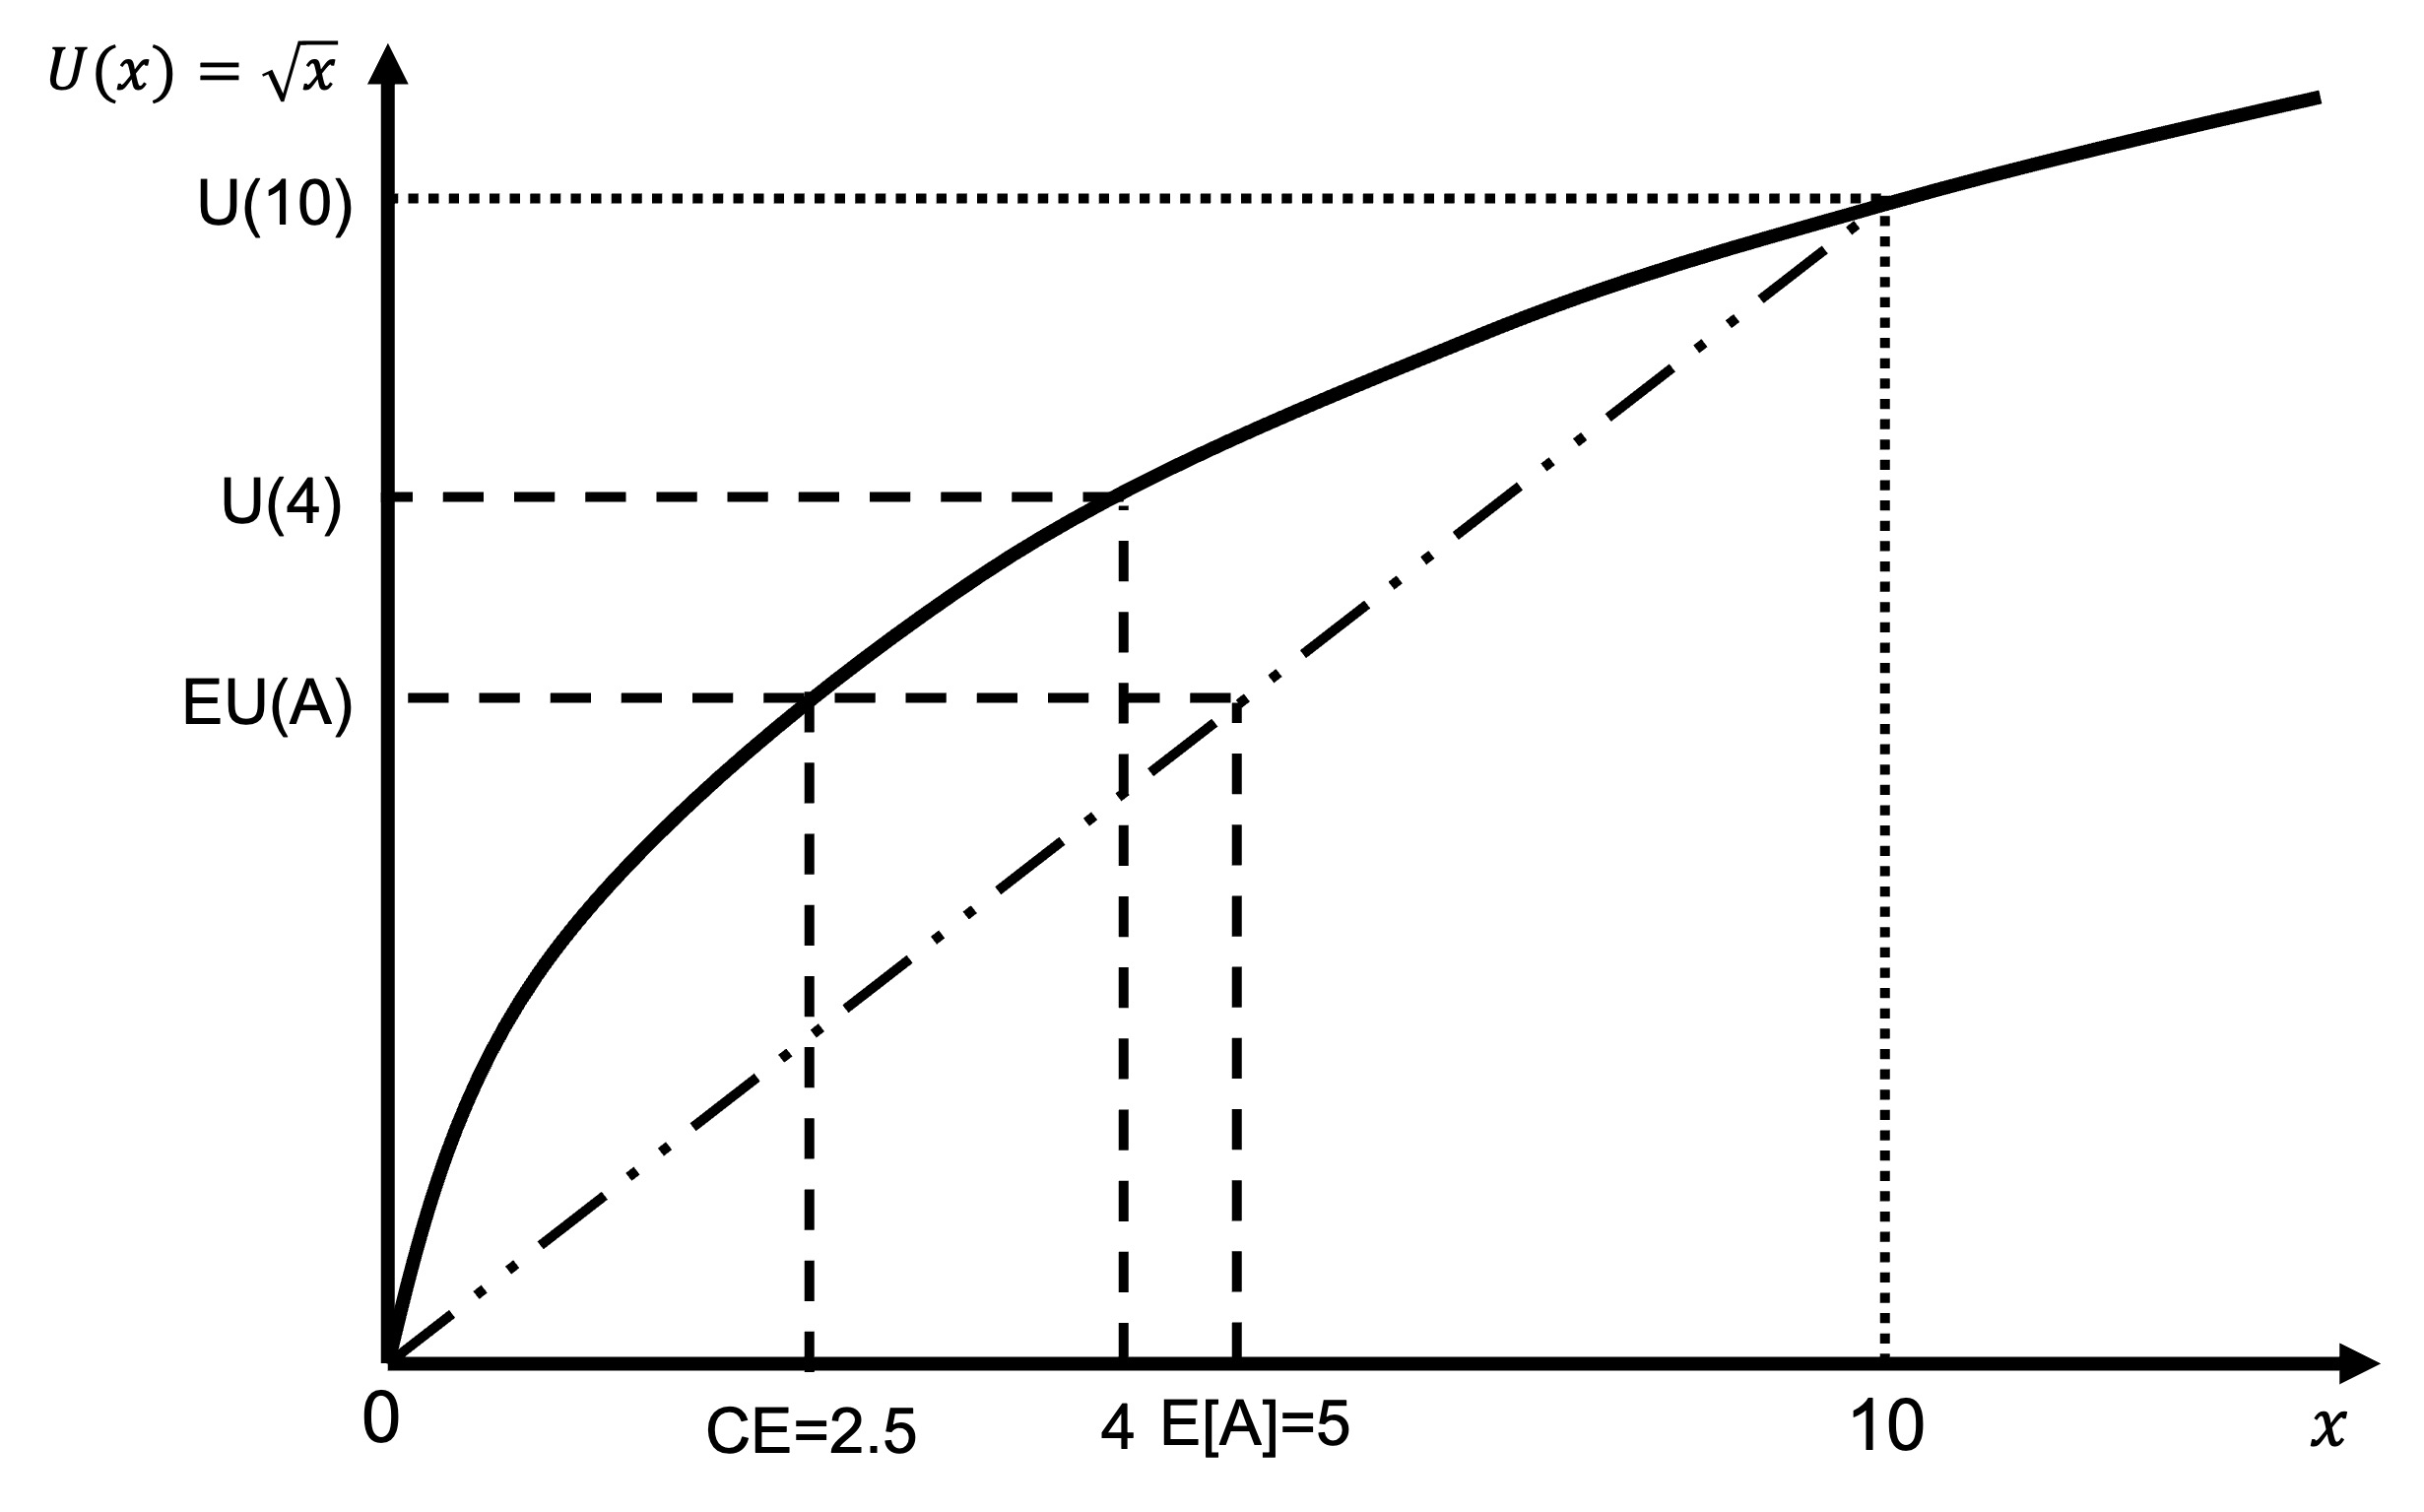
\includegraphics{risk-and-uncertainty/img/expected-utility-exercises-question-1.jpg}

\end{tcolorbox}

\hypertarget{a-5050-gamble}{%
\section{A 50:50 gamble}\label{a-5050-gamble}}

Consider the following gamble:

\begin{quote}
(0.5; \$550; 0.5, -\$500)
\end{quote}

This gamble provides a 50\% chance of winning \$550 and a 50\% chance of
losing \$500.

a) Would a risk neutral agent (who maximises expected value) be willing
to pay \$20 to play this gamble? What is the most they would be willing
to pay to play?

\begin{tcolorbox}[enhanced jigsaw, title=\textcolor{quarto-callout-tip-color}{\faLightbulb}\hspace{0.5em}{Answer}, toprule=.15mm, colback=white, breakable, titlerule=0mm, colframe=quarto-callout-tip-color-frame, coltitle=black, opacityback=0, rightrule=.15mm, colbacktitle=quarto-callout-tip-color!10!white, bottomtitle=1mm, opacitybacktitle=0.6, arc=.35mm, bottomrule=.15mm, toptitle=1mm, leftrule=.75mm, left=2mm]

The expected value of the gamble is:

\begin{align*}
E[X]&=\sum_{i=1}^n p_ix_i \\[12pt]
&=0.5(550)+0.5(-500) \\[6pt]
&=25
\end{align*}

This is greater than \$20, so a risk neutral agent will be willing to
pay \$20 to participate in the gamble.

We could also have solved this by determining the expected value if they
had paid \$20:

\begin{align*}
E[X]-c&=\sum_{i=1}^n p_ix_i-c \\[12pt]
&=0.5(550)+0.5(-500)-20 \\[6pt]
&=5
\end{align*}

As the expected value is positive, the agent would be willing to pay
\$20.

\end{tcolorbox}

b) Would a risk averse expected utility maximiser with wealth \$1000 and
utility function \(U(x)=x^{1/2}\) be willing to pay \$20 to play this
gamble? What is the most they would be willing to pay to play?

\begin{tcolorbox}[enhanced jigsaw, title=\textcolor{quarto-callout-tip-color}{\faLightbulb}\hspace{0.5em}{Answer}, toprule=.15mm, colback=white, breakable, titlerule=0mm, colframe=quarto-callout-tip-color-frame, coltitle=black, opacityback=0, rightrule=.15mm, colbacktitle=quarto-callout-tip-color!10!white, bottomtitle=1mm, opacitybacktitle=0.6, arc=.35mm, bottomrule=.15mm, toptitle=1mm, leftrule=.75mm, left=2mm]

The expected utility of the gamble for the risk averse agent if they
paid \$20 to play is:

\begin{align*}
EU(x)&=p_1(W+x_1-c)+p_2(W+x_2-c) \\[6pt]
&=0.5(1000+550-20)^{1/2}+0.5(1000-500-20)^{1/2} \\[6pt]
&=30.51
\end{align*}

The expected utility of not playing the gamble is:

\begin{align*}
EU(x)&=(1000)^{1/2} \\[6pt]
&=31.62
\end{align*}

They would not pay \$20 as they would have higher utility if they turned
down the gamble.

In fact, they would not pay any positive sum to participate in the
gamble. If they were offered the gamble for free, their expected utility
would be:

\begin{align*}
EU(x)&=0.5(1000+550)^{1/2}+0.5(1000-500)^{1/2} \\[6pt]
&=30.86
\end{align*}

This is less than if they simply turned down the gamble. They would be
willing to pay to avoid the gamble. How much?

We can determine this by asking what wealth a utility of 30.86 is:

\begin{align*}
W^{1/2}&=30.86 \\[6pt]
W&=30.51^2 \\[6pt]
&=\$952.67
\end{align*}

The certainty equivalent of the gamble is \$952.67. The agent would be
willing to pay up to \$47.33 to avoid the gamble.

\end{tcolorbox}

c) Would the expected utility maximiser with utility function
\(U(x)=x^{1/2}\) change their decision if they had \$1 million in
wealth? Explain.

\begin{tcolorbox}[enhanced jigsaw, title=\textcolor{quarto-callout-tip-color}{\faLightbulb}\hspace{0.5em}{Answer}, toprule=.15mm, colback=white, breakable, titlerule=0mm, colframe=quarto-callout-tip-color-frame, coltitle=black, opacityback=0, rightrule=.15mm, colbacktitle=quarto-callout-tip-color!10!white, bottomtitle=1mm, opacitybacktitle=0.6, arc=.35mm, bottomrule=.15mm, toptitle=1mm, leftrule=.75mm, left=2mm]

If they now have \$1 million in wealth, we simply repeat the
calculations above with the new wealth.

\begin{align*}
EU(x)&=0.5(1000000+550-20)^{1/2}+0.5(1000000-500-20)^{1/2} \\[6pt]
&=1000.00247
\end{align*}

The expected utility of not playing the gamble is:

\begin{align*}
EU(x)&=(1000000)^{1/2} \\[6pt]
&=1000
\end{align*}

They would be willing to pay \$20 as they would have higher utility if
they accepted the gamble.

What is the most they would be willing to pay? If they were offered the
gamble for free, their expected utility would be:

\begin{align*}
EU(x)&=0.5(1000000+550)^{1/2}+0.5(1000000-500)^{1/2} \\[6pt]
&=1000.0125
\end{align*}

How much would they be willing to pay for this opportunity? We can
determine this by asking what wealth a utility of 1000.0125 is:

\begin{align*}
W&=(1000.0124655)^2 \\[6pt]
&=\$1000024.93
\end{align*}

The agent would be willing to pay up to \$24.93 for the gamble. This is
close to the expected value of \$25.

Intuitively, as the agent's wealth increases their utility function
becomes increasingly linear (second derivative approaches zero) and they
become closer to risk neutral.

\end{tcolorbox}

\hypertarget{a-6040-gamble}{%
\section{A 60:40 gamble}\label{a-6040-gamble}}

Penny is an expected utility maximiser with utility function
\(u(x)=ln(x)\) and wealth of \$300.

Penny is offered the following bet A:

\begin{itemize}
\tightlist
\item
  a 60\% probability to win \$150
\item
  a 40\% probability to lose \$100.
\end{itemize}

a) Does Penny accept bet A?

\begin{tcolorbox}[enhanced jigsaw, title=\textcolor{quarto-callout-tip-color}{\faLightbulb}\hspace{0.5em}{Answer}, toprule=.15mm, colback=white, breakable, titlerule=0mm, colframe=quarto-callout-tip-color-frame, coltitle=black, opacityback=0, rightrule=.15mm, colbacktitle=quarto-callout-tip-color!10!white, bottomtitle=1mm, opacitybacktitle=0.6, arc=.35mm, bottomrule=.15mm, toptitle=1mm, leftrule=.75mm, left=2mm]

Penny compares the utility of taking versus not taking the bet:

\begin{align*}
U(\text{A})&=p_1u(x_1)+p_2u(x_2) \\
&=0.6ln(W+150)+0.4ln(W-100) \\
&=0.6ln(450)+0.4ln(200) \\
&=5.785 \\
\\
U(W)&=ln(W) \\
&=ln(300) \\
&=5.704
\end{align*}

\(U(A)>U(W)\), so Penny accepts the bet.

\end{tcolorbox}

b) Following some bad economic news, Penny wealth declines to \$150.

Penny is offered bet A again. Does Penny accept the bet?

\begin{tcolorbox}[enhanced jigsaw, title=\textcolor{quarto-callout-tip-color}{\faLightbulb}\hspace{0.5em}{Answer}, toprule=.15mm, colback=white, breakable, titlerule=0mm, colframe=quarto-callout-tip-color-frame, coltitle=black, opacityback=0, rightrule=.15mm, colbacktitle=quarto-callout-tip-color!10!white, bottomtitle=1mm, opacitybacktitle=0.6, arc=.35mm, bottomrule=.15mm, toptitle=1mm, leftrule=.75mm, left=2mm]

Penny compares the utility of taking versus not taking the bet:

\begin{align*}
U(\text{A})&=p_1u(x_1)+p_2u(x_2) \\
&=0.6ln(W+150)+0.4ln(W-100) \\
&=0.6ln(300)+0.4ln(50) \\
&=4.987 \\
\\
U(W)&=ln(W) \\
&=ln(150) \\
&=5.011
\end{align*}

\(U(A)<U(W)\), so Penny rejects the bet.

\end{tcolorbox}

\hypertarget{another-6040-gamble}{%
\section{Another 60:40 gamble}\label{another-6040-gamble}}

Gamble A is as follows:

(\$100, 0.6; -\$100, 0.4)

This is a gamble with a 60\% chance of winning \$100 and a 40\% chance
of losing \$100.

a) Would a risk neutral decision-maker (who maximises expected value) be
willing to pay \$10 to play gamble A? What is the most they would be
willing to pay to play?

\begin{tcolorbox}[enhanced jigsaw, title=\textcolor{quarto-callout-tip-color}{\faLightbulb}\hspace{0.5em}{Answer}, toprule=.15mm, colback=white, breakable, titlerule=0mm, colframe=quarto-callout-tip-color-frame, coltitle=black, opacityback=0, rightrule=.15mm, colbacktitle=quarto-callout-tip-color!10!white, bottomtitle=1mm, opacitybacktitle=0.6, arc=.35mm, bottomrule=.15mm, toptitle=1mm, leftrule=.75mm, left=2mm]

A risk neutral decision maker will accept any offer with positive
expected value. The expected value of the bet is:

\begin{align*}
E[A]&=p_1x_1+p_2x_2 \\
&=0.6*100+0.4*(-100) \\
&=\$20
\end{align*}

The risk neutral decision maker would pay \$10 as this is less than the
expected value of the bet. They would be willing to pay up to the
expected value of the bet: \$20. At that point they would be indifferent
between paying for the bet and refusing the bet.

\end{tcolorbox}

b) Would an expected utility maximiser with wealth \$200 and utility
function \(U(x)=ln(x)\) be willing to pay \$10 to play gamble A? What is
the most they would be willing to pay to play?

\begin{tcolorbox}[enhanced jigsaw, title=\textcolor{quarto-callout-tip-color}{\faLightbulb}\hspace{0.5em}{Answer}, toprule=.15mm, colback=white, breakable, titlerule=0mm, colframe=quarto-callout-tip-color-frame, coltitle=black, opacityback=0, rightrule=.15mm, colbacktitle=quarto-callout-tip-color!10!white, bottomtitle=1mm, opacitybacktitle=0.6, arc=.35mm, bottomrule=.15mm, toptitle=1mm, leftrule=.75mm, left=2mm]

The expected utility maximiser will play if their utility from playing
and paying is greater than their utility of refusing.

\begin{align*}
U(W)&=ln(W) \\
&=ln(\$200) \\
&=5.2983174 \\
\\
E[U(A-c)]&=p_1U(x_1)+p_2U(x_2) \\
&=0.6U(W+100-10)+0.4U(W-100-10) \\
&=0.6ln(200+100-10)+0.4ln(200-100-10) \\
&=5.2018524
\end{align*}

\(U(W)>U(A-c)\) so the decision maker will not be willing to pay \$10.

To determine the most they would be willing to pay, we will first check
whether they will pay any positive sum. We will do that by examining the
expected utility of the gamble with no payment.

\begin{align*}
E[U(A)]&=p_1U(x_1)+p_2U(x_2) \\
&=0.6U(W+100)+0.4U(W-100) \\
&=0.6ln(200+100)+0.4ln(200-100) \\
&=5.2643376
\end{align*}

\(U(W)>U()\) so the decision maker will not be willing to pay any
amount. In fact, they would pay to avoid the bet.

To calculate how much, we determine what the certainty equivalent of the
bet is:

\begin{align*}
U(CE)&=E[U(A)] \\
ln(CE)&=5.2643376\\
CE&=e^{5.2643376} \\
&=\$
\end{align*}

Having wealth of \$200 and the bet is the equivalent of having wealth of
\$193.32. They would be willing to pay up to \$6.68 to avoid the bet.

\end{tcolorbox}

c) Would the expected utility maximiser with utility function change
their decision if they had \$1000 in wealth? Explain.

\begin{tcolorbox}[enhanced jigsaw, title=\textcolor{quarto-callout-tip-color}{\faLightbulb}\hspace{0.5em}{Answer}, toprule=.15mm, colback=white, breakable, titlerule=0mm, colframe=quarto-callout-tip-color-frame, coltitle=black, opacityback=0, rightrule=.15mm, colbacktitle=quarto-callout-tip-color!10!white, bottomtitle=1mm, opacitybacktitle=0.6, arc=.35mm, bottomrule=.15mm, toptitle=1mm, leftrule=.75mm, left=2mm]

The expected utility maximiser will play if their utility from playing
and paying is greater than their utility of refusing.

\begin{align*}
U(W)&=ln(W) \\
&=ln(\$1000) \\
&=6.9077553 \\
\\
E[U(A-c)]&=p_1U(x_1)+p_2U(x_2) \\
&=0.6U(W+100-10)+0.4U(W-100-10) \\
&=0.6ln(1000+100-10)+0.4ln(1000-100-10) \\
&=6.9128484
\end{align*}

\(U(W)<U(A-c)\) so the decision maker is now willing to pay \$10.

As the agent's wealth increases their utility function becomes
increasingly linear (second derivative approaches zero) and they become
closer to risk neutral. As a result, the positive expected value bet
becomes increasingly attractive.

\end{tcolorbox}

d) At what wealth is the expected utility maximiser with utility
function \(U(x)=ln(x)\) indifferent between accepting gamble A or not?

\begin{tcolorbox}[enhanced jigsaw, title=\textcolor{quarto-callout-tip-color}{\faLightbulb}\hspace{0.5em}{Answer}, toprule=.15mm, colback=white, breakable, titlerule=0mm, colframe=quarto-callout-tip-color-frame, coltitle=black, opacityback=0, rightrule=.15mm, colbacktitle=quarto-callout-tip-color!10!white, bottomtitle=1mm, opacitybacktitle=0.6, arc=.35mm, bottomrule=.15mm, toptitle=1mm, leftrule=.75mm, left=2mm]

The expected utility maximiser will be indifferent when:

\begin{align*}
U(W)&=E[U(A)] \\
U(W)&=0.6U(W+100)+0.4U(W-100) \\
ln(W)&=0.6ln(W+100)+0.4ln(W-100)
\end{align*}

There isn't a simple closed form solution to this equation, but we know
from questions b) and c) that \(W\) is somewhere between \$200 and
\$1000.

If we wanted to calculate exact solution, you could use tool such as
Mathematica or Matlab to solve, write a short code to solve in R or even
iterate toward a solution using Excel. Below is example code in R.

The expected utility maximiser is indifferent when \(W=\)\$256.81.

\end{tcolorbox}

\hypertarget{purchasing-insurance}{%
\section{Purchasing insurance}\label{purchasing-insurance}}

An agent is considering insurance against bushfire for its \$1,000,000
house. The house has a 1 in 1000 chance of burning down. An insurer is
willing to offer full coverage for \$1100.

a) Would a risk neutral agent purchase the insurance?

\begin{tcolorbox}[enhanced jigsaw, title=\textcolor{quarto-callout-tip-color}{\faLightbulb}\hspace{0.5em}{Answer}, toprule=.15mm, colback=white, breakable, titlerule=0mm, colframe=quarto-callout-tip-color-frame, coltitle=black, opacityback=0, rightrule=.15mm, colbacktitle=quarto-callout-tip-color!10!white, bottomtitle=1mm, opacitybacktitle=0.6, arc=.35mm, bottomrule=.15mm, toptitle=1mm, leftrule=.75mm, left=2mm]

We have already calculated that purchasing insurance in this case has a
lower expected value than not purchasing the insurance. A risk neutral
agent would not purchase the insurance.

\end{tcolorbox}

b) Suppose an agent has a logarithmic utility function (\(U(x)=\ln(x)\))
and they have \$10,000 in cash in addition to their house, giving them
wealth (\(W\)) of \$1,010,000. Would this agent purchase the insurance?
Are they risk seeking, risk neutral or risk averse?

\begin{tcolorbox}[enhanced jigsaw, title=\textcolor{quarto-callout-tip-color}{\faLightbulb}\hspace{0.5em}{Answer}, toprule=.15mm, colback=white, breakable, titlerule=0mm, colframe=quarto-callout-tip-color-frame, coltitle=black, opacityback=0, rightrule=.15mm, colbacktitle=quarto-callout-tip-color!10!white, bottomtitle=1mm, opacitybacktitle=0.6, arc=.35mm, bottomrule=.15mm, toptitle=1mm, leftrule=.75mm, left=2mm]

\begin{align*}
E[U(\text{purchase})]&=\ln(W-premium) \\
&=\ln(1,008,900) \\
&=13.8244\\
\\
E[U(\text{don't})]&=0.999*\ln(W)+0.001*\ln(W-value_{\text{house}}) \\
&=0.999*\ln(1,010,000)+0.001*\ln(10,000) \\
&=13.8208
\end{align*}

The expected utility of purchasing insurance is greater than the
expected utility from not purchasing insurance. This agent will purchase
insurance. They are risk averse.

What is the intuition for this agent's purchase of insurance?
Diminishing marginal utility means that the utility of average wealth is
greater than the average utility of wealth
(e.g.~\(U(\$0)+U(\$200)<U(\$100)+U(\$100)\)). Therefore, their expected
utility is higher when wealth is distributed evenly across the possible
states of the world rather than concentrated in one state - or in the
case of a disaster, very low in one state. The consumer insures as a way
of evenly distributing wealth across all possible states.

\end{tcolorbox}

\hypertarget{insurance-but-not-a-lottery-ticket}{%
\section{Insurance but not a lottery
ticket}\label{insurance-but-not-a-lottery-ticket}}

In your own words but using concepts from this subject explain why a
risk averse agent who makes decisions according to expected utility
theory might purchase insurance but not a lottery ticket.

\begin{tcolorbox}[enhanced jigsaw, title=\textcolor{quarto-callout-tip-color}{\faLightbulb}\hspace{0.5em}{Answer}, toprule=.15mm, colback=white, breakable, titlerule=0mm, colframe=quarto-callout-tip-color-frame, coltitle=black, opacityback=0, rightrule=.15mm, colbacktitle=quarto-callout-tip-color!10!white, bottomtitle=1mm, opacitybacktitle=0.6, arc=.35mm, bottomrule=.15mm, toptitle=1mm, leftrule=.75mm, left=2mm]

Both lotteries and insurance have a negative expected value.

The risk averse agent will typically reject a lottery as it has a small
probability of a large win for the price of a small loss. Due to
diminishing marginal returns, the average weight given to each dollar in
the large gain is weighted much less than the average weight given to
each dollar in the small price. This makes the lottery unattractive.

In contrast, a risk averse agent may purchase insurance as for a small
price they can avoid the possibility of a large loss. Due to diminishing
marginal returns, the large loss can have much higher average weight
given to each dollar than to the weight given to each dollar for the
small premium.

\end{tcolorbox}

\hypertarget{an-anomaly-in-expected-utility}{%
\section{An anomaly in expected
utility}\label{an-anomaly-in-expected-utility}}

Consider the following two choices:

\textbf{Choice 1}: Choose one of the following bets:

Bet A:

\begin{itemize}
\tightlist
\item
  \$10,000 with probability: 11\%
\item
  \$0 with probability: 89\%
\end{itemize}

Bet B:

\begin{itemize}
\tightlist
\item
  \$50,000 with probability: 10\%
\item
  \$0 with probability: 90\%
\end{itemize}

\textbf{Choice 2}: Choose one of the following bets:

Bet A':

\begin{itemize}
\tightlist
\item
  \$10,000 with probability: 100\%
\end{itemize}

Bet B':

\begin{itemize}
\tightlist
\item
  \$50,000 with probability: 10\%
\item
  \$10,000 with probability: 89\%
\item
  \$0 with probability: 1\%
\end{itemize}

Many people pick B for Choice 1 and A' for Choice 2.

Does this pair of choices conform with Expected Utility Theory? Why?

\begin{tcolorbox}[enhanced jigsaw, title=\textcolor{quarto-callout-tip-color}{\faLightbulb}\hspace{0.5em}{Answer}, toprule=.15mm, colback=white, breakable, titlerule=0mm, colframe=quarto-callout-tip-color-frame, coltitle=black, opacityback=0, rightrule=.15mm, colbacktitle=quarto-callout-tip-color!10!white, bottomtitle=1mm, opacitybacktitle=0.6, arc=.35mm, bottomrule=.15mm, toptitle=1mm, leftrule=.75mm, left=2mm]

According to Expected Utility Theory, if an agent selects B:

\begin{align*}
0.10U(50,000)+0.90U(0)&> 0.11U(10,000)+ 0.89U(0) \\[6pt]
0.10U(50,000)+0.01U(0)&> 0.11U(10,000)
\end{align*}

According to Expected Utility Theory, if an agent selects A':

\begin{align*}
U(10,000)&>0.10U(50,000)+0.89U(10,000)+0.01U(0) \\[6pt]
0.11U(10,000)&>0.89U(50,000)+0.01U(0)
\end{align*}

This is a contradiction. Under expected utility theory, if an agent
chooses B it should choose B'. And if the agent chooses A it should
choose A'.

This occurs due to a breach in the principle of independence.

Here is a representation of the choices.

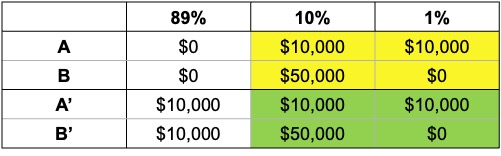
\includegraphics{risk-and-uncertainty/img/allais-paradox-4.jpg}

The bets in the two shaded areas are the same. They are paired with an
outcomes of either \$10,000 or \$0. Preferring B to A and A' to B' is a
violation of the axiom of the \href{@sec-independence}{independence of
irrelevant alternatives}: Under that axiom, two gambles mixed with an
irrelevant third gamble will maintain the same order of preference as
when the two are presented independently of the third gamble.

Using this representation in the table, here is another way of
understanding why this combination of choices is an anomaly. Imagine
there are 100 tickets numbered 1 to 100. One ticket will be drawn. If a
ticket between 1 and 89 is drawn, you win the prize in the first column.
If a ticket between 90 and 99 is drawn, you win the amount in the
second. If a 100 is drawn, you win the sum in the third.

Suppose that you know the ticket that is drawn is between 1 and 89.
Would you prefer A or B? As you would win \$0 with either choice, you
will be indifferent. You will similarly be indifferent between A' and
B', winning \$10,00 no matter what.

Suppose instead that a ticket between 90 and 100 is drawn, but you know
which. You can see that if you prefer A to B, you should also prefer A'
to B'. In each choice you are effectively facing the same bet. Let's
assume for the moment that you prefer B and B'.

Finally, suppose you don't know what ticket will be drawn. We have just
determined that if you know the ticket is between 1 and 89 you are
indifferent between the options, but if between 90 and 100 is drawn you
prefer B and B'. You do not prefer A or A' when the ticket range is 1 to
89 or 90 to 100, so you should not prefer A or A' when the ticket number
is unknown.

Finally, using the formal definition for the independence of irrelevant
alternatives axiom:

\begin{itemize}
\tightlist
\item
  if \(x\) and \(y\) are lotteries with \(x\succcurlyeq y\) and
\item
  \(p\) is the probability that a third option \(z\) is present, then:
  \[
  pz+(1-p)x\succcurlyeq pz+(1-p)y
  \]
\end{itemize}

For each of the choices in our lottery:

\begin{itemize}
\item
  \(p=89\%\)
\item
  \(x\) is a 100\% chance of \$10,000
\item
  \(y\) is a 0.01/(1-0.89) chance of \$0 and 0.10/(1-0.89) chance of
  \$50,000
\item
  \(z\) is \$10,000 in choice 1 and \$0 in choice 2, although \(z\)'s
  value does not matter due to its assumed irrelevance.
\end{itemize}

\end{tcolorbox}

\part{Prospect theory}

Kahneman and Tversky (1979) challenged Expected Utility Theory by
introducing a new descriptive theory they called Prospect Theory that
addresses the anomalies that we identified in the previous part.

Prospect theory has the following features:

\begin{itemize}
\tightlist
\item
  A value function that incorporates:

  \begin{itemize}
  \tightlist
  \item
    Reference dependence
  \item
    Loss aversion
  \item
    The reflection effect
  \end{itemize}
\item
  Probability weighting
\end{itemize}

I will address each of these features individually before combining
them.

\hypertarget{reference-dependence}{%
\chapter{Reference dependence}\label{reference-dependence}}

Under Prospect Theory, people assess choices based on a reference point,
as opposed to an absolute assessment of their position. Outcomes are
coded as losses and gains relative to that reference point.

The earlier example of assessing a share portfolio worth \$30,000 from a
reference point of either \$20,000 or \$40,000 is an example of
reference dependence.

Under expected utility theory, utility is typically thought of as being
the product of your entire wealth (\(W\)). For example, if you gain
\$100, your utility increases from \(u(W)\) to \(u(W+\$100)\).

In contrast, under prospect theory, the value function (what the utility
function is typically called in Prospect Theory) applies to changes
relative to the reference point. If their initial reference point is
their wealth before receiving the \$100, the value of that change is
\(v(\$100)\). The importance of that distinction becomes apparent when
we consider how people consider losses and gains.

\hypertarget{theories-of-reference-depdendence}{%
\section{Theories of reference
depdendence}\label{theories-of-reference-depdendence}}

There are a number of theories on reference point formation. These
include:

\begin{itemize}
\tightlist
\item
  The status quo
\item
  Lagged consumption
\item
  Goals
\item
  Recent expectations
\end{itemize}

\hypertarget{the-status-quo}{%
\subsection{The status quo}\label{the-status-quo}}

A common assumption in Prospect Theory is that the reference point is
the status quo (as it was for many examples in the original paper by
Kahneman and Tversky (1979)). The status quo implies a preference for
the current state. Any negative change is perceived as a loss.

The status quo appears straightforward and has been shown to be
effective in contexts such as lab experiments.

However, the status quo as a reference point does not appear to be a
useful assumption for describing many economic interactions. Suppose you
decide to sell your bike. Do you see the foregoing of the bike as a
loss?

What is you run a bike shop? Does every sale involve a feeling of loss?
For markets in which intangible and fungible goods are exchanged
(e.g.~stock market) the status quo assumption appears a poor fit.

\hypertarget{lagged-consumption}{%
\subsection{Lagged consumption}\label{lagged-consumption}}

Imagine you win the lottery.

How do you feel one week after the draw?

How do you feel one year after the draw?

Your reference point likely reflects more recent consumption.

Lagged consumption introduces adaptation into reference point
determination:

\begin{enumerate}
\def\labelenumi{\arabic{enumi}.}
\tightlist
\item
  We react to shocks
\item
  The effect of the shock fades in time
\end{enumerate}

\hypertarget{goals}{%
\subsection{Goals}\label{goals}}

Consider the following problem from Heath et al. (1999):

\begin{quote}
Sally and Trish both follow workout plans that usually involve doing 25
sit-ups.

One day, Sally sets a goal of performing 31 sit-ups. She finds herself
very tired after performing 35 sit-ups and stops.

Trish sets a goal of performing 39 sit-ups. She finds herself very tired
after per- forming 35 sit-ups and stops.

What emotion is each person experiencing?
\end{quote}

With goals as reference points, people see success or failure to achieve
a goal as a loss or gain. Although both have the same performance, Sally
will have a positive emotional reaction and Trish a negative reaction.

\hypertarget{recent-expectations}{%
\subsection{Recent expectations}\label{recent-expectations}}

In this approach, the reference point is beliefs about future outcomes
(Kőszegi and Rabin (2006)). For example, a 5\% pay rise when expecting a
10\% pay rise may be perceived as a loss.

The expectations-based theory can produce the same predictions of
alternative theories:

\begin{enumerate}
\def\labelenumi{\arabic{enumi}.}
\tightlist
\item
  Status-quo: if expectations are stable, recent expectations will
  reflect the status quo
\item
  Lagged consumption: recent consumption will shape expectations
\item
  Goals: goals can shape (or be shaped by) expectations
\end{enumerate}

\hypertarget{loss-aversion}{%
\chapter{Loss aversion}\label{loss-aversion}}

Loss aversion is the concept that losses loom larger than gains. People
feel more strongly about a loss than they do an equivalent gain, so are
often willing to reject gambles with a materially positive expected
value.

Loss aversion can explain why we behave differently depending on whether
the decision making induces a gain or a loss.

For instance, if someone feels losses with twice the feeling of gains, a
50:50 bet to win \$550, lose \$500 will be unattractive. This provides
an alternative explanation to the absurd levels of risk aversion
required to reject this bet (as discussed in Section~\ref{sec-absurd}).

\hypertarget{a-value-function-with-loss-aversion}{%
\section{A value function with loss
aversion}\label{a-value-function-with-loss-aversion}}

The following is an example of a value function with loss aversion:

\[
v(x)=\left\{\begin{matrix}
x \space &\textrm{where} \space x \geq 0\\
2x \space &\textrm{where} \space x<0
\end{matrix}\right.
\]

where \(x\) is the outcome relative to the reference point.

For example, suppose someone is given \$100. If their initial reference
point is their wealth before receiving the \$100, \(x\) will be \$100.
Therefore their utility is +100. If the same person instead loses \$100,
their utility would be -200.

The following plot shows the increased effect of the loss under this
value function:

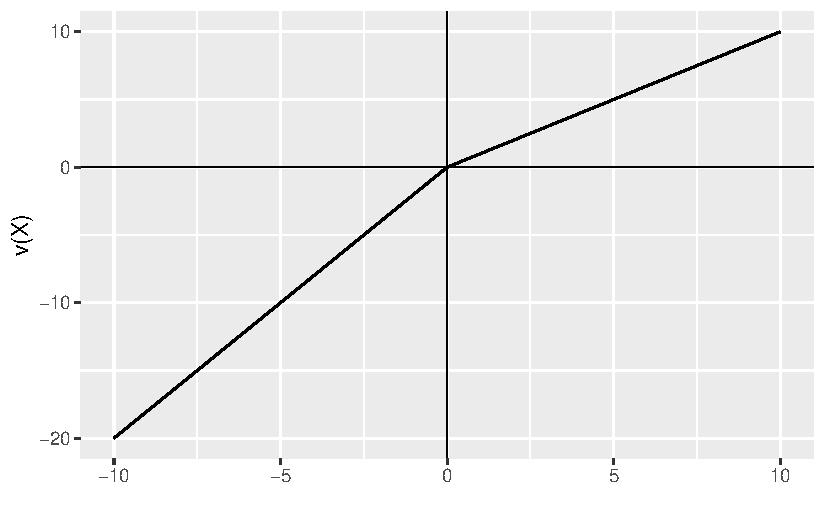
\includegraphics{prospect-theory/loss-aversion_files/figure-pdf/unnamed-chunk-1-1.pdf}

The kink where the axes intercept is representative of the greater
effect of losses.

\hypertarget{the-endowment-effect}{%
\section{The endowment effect}\label{the-endowment-effect}}

Kahneman et al. (1991) ran one of the most famous and replicated
experiments in economics.

They randomly assigned a free mug to members of a group and asked how
much money they would accept for returning the mug (i.e.~willingness to
accept). The remaining participants were only shown a mug and asked
their willingness to pay for the mug.

Kahneman et al. (1991) found that the willingness to accept (\$5.75) was
substantially higher than the willingness to pay (\$2.25).

This experiment has been replicated in real estate markets, the stock
market, with basketball tickets and in other domains.

The endowment effect is this phenomena where people impute additional
value to the items they own. The endowment effect is argued to be an
empirical expression of loss aversion. Willingness to accept is higher
as it is payment to incur the loss of the mug.

\hypertarget{endowment-effect-example}{%
\subsection{Endowment effect example}\label{endowment-effect-example}}

Bruce has the following reference-dependent value function:

\[
v(x)=\left\{\begin{matrix}
x \space &\textrm{where} \space x \geq 0\\
2x \space &\textrm{where} \space x<0
\end{matrix}\right.
\]

where \(x\) is the outcome relative to the reference point.

Assume Bruce has preferences over money (\(m\)) and mugs (\(c\)) as
follows:

\[
V(x)=v(m-r_m)+v(5c-5r_c)
\]

Where \(r_m\) is his reference point as it relates to money and \(r_c\)
is his reference point as it relates to mugs.

At the beginning of the experiment Bruce is given a mug. Assuming
Bruce's reference point adapts such that he considers the mug his, how
much would Bruce need to be paid to give up the mug?

\begin{align*}
V(x)&=v(m-r_m)+v(5c-5r_c) \\
&=v(W+p-W)+v(5\times 0-5\times 1) \\
&=v(p)+v(-5) \\
&=p-2\times 5 \\
&=p-10
\end{align*}

Bruce would need to be paid at least \$10 to give up the mug. Giving up
the mug is seen as a loss and given greater weight than the money
gained. Otherwise he would experience negative value.

Now assume Bruce was not given a mug, but rather an opportunity to
purchase a mug. How much would Bruce be willing to pay for the mug?

\begin{align*}
V(x)&=v(m-r_m)+v(5c-5r_c) \\
&=v(W-p-W)+v(5\times 1-5\times 0) \\
&=v(-p)+v(5) \\
&=2p-5
\end{align*}

The most Bruce would be willing to pay for the mug is \$2.50. He sees
the foregone money as a loss, so it is given greater weight than the mug
gained.

\hypertarget{the-reflection-effect}{%
\chapter{The reflection effect}\label{the-reflection-effect}}

When people make a risky choice related to gains, they are risk averse.
They prefer a certain option with lower expected utility than the
expected utility of the risky choice. When making a choice in the loss
domain, they become risk seeking. This phenomena is called the
reflection effect.

This phenomena might also be thought of as diminishing sensitivity to
gains or losses in either direction. This contrasts with expected
utility theory where the pain of losses increases as they grow in size.

The reflection effect provides an explanation for the framing effects we
observed in the question about the unusual disease. In the gain frame,
the preferred option is risk averse. In the loss frame, the preferred
option tends to be the risk seeking option.

\hypertarget{the-reflection-effect-in-the-value-function}{%
\section{The reflection effect in the value
function}\label{the-reflection-effect-in-the-value-function}}

The following value function is an example of a function where there is
diminishing sensitivity to both gains and losses.

\begin{equation*}
v(x)= \Bigg\{
\begin{matrix}
x^\frac{1}{2} \space \text{where} \space x \geq 0\\
-(-x)^\frac{1}{2} \space \text{where} \space x<0
\end{matrix}
\end{equation*}

As \(x\) increases in magnitude in either direction, the marginal
increase in value from each additional unit of \(x\) decreases.

The result of this is risk averse behaviour in the gain domain and risk
seeking behaviour in the loss domain. The following plot shows the
diminishing effect in each direction.

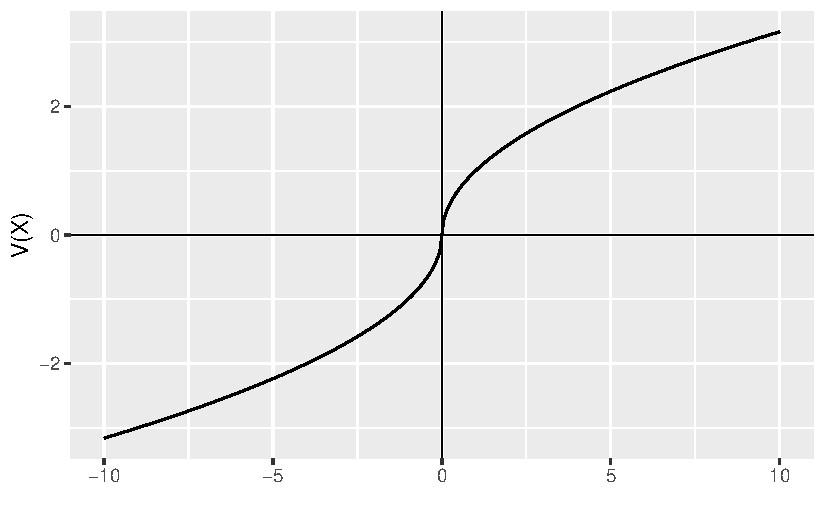
\includegraphics{prospect-theory/reflection-effect_files/figure-pdf/unnamed-chunk-1-1.pdf}

In the gain domain the function is convex, indicating risk aversion. In
the loss domain the concave function indicates risk seeking behaviour.

The following numerical example illustrates further.

Suppose an agent with the above value function is offered a choice
between \$10 for certain and a 50:50 bet to win \$20 or end up with
nothing. The value of each choice is:

\begin{align*}
v(\text{certainty})&=v(10) \\
&=10^{\frac{1}{2}} \\
&=3.1622777 \\
\\
v(\text{bet})&=0.5*v(20)+0.5*v(0) \\
&=0.5*20^{\frac{1}{2}}+0.5*0 \\
&=2.236068
\end{align*}

The \$10 for certain has a higher value for the agent. This agent is
risk averse in the gain domain and therefore prefers an amount for
certainty over a bet with the same expected value.

Suppose the agent is now offered another choice. They can now have a
certain loss of \$10 or a 50:50 bet to lose \$20 or to lose nothing. The
value of each choice is:

\begin{align*}
v(\text{certainty})&=v(-10) \\
&=-10^{\frac{1}{2}} \\
&=-3.1622777 \\
\\
v(\text{bet})&=0.5*v(-20)+0.5*v(0) \\
&=-0.5*20^{\frac{1}{2}}+0.5*0 \\
&=-2.236068
\end{align*}

This bet delivers higher value than the certain loss, despite the bet
and the certain loss having the same expected value. The agent is
willing to take a risk to avoid a loss. They are risk seeking in the
loss domain.

\hypertarget{the-value-function}{%
\chapter{The value function}\label{the-value-function}}

These three phenomena: reference dependence loss aversion and the
reflection effect are reflected in the Prospect Theory value function in
the following way:

1. The value function of Prospect Theory is defined on changes in wealth
or welfare, rather than on final wealth levels. In other words, gains
and losses are defined relative to a reference point. The reference
point can be current wealth, a social or psychological status quo, or an
expectation about the outcome.

Utility from an outcome depends on distance to the relevant reference
level. A multi-millionaire may not accept a 50:50 bet to win \$550, lose
\$500 because they are not comparing to their total wealth but relative
to the reference point of the status quo.

2. Perceptions of both gains and losses are characterised by diminishing
marginal sensitivity in either direction. Successive incremental changes
have a smaller marginal impact.

This is similar to decreasing marginal utility to wealth of expected
utility theory. The two differ in the baseline. In expected utility
theory, the starting value is zero wealth, with increases from there
decreasing in marginal utility. In prospect theory, the starting value
is the reference point, with both increases and decreases having smaller
marginal effect as they increase in magnitude.

3. Losses loom larger than gains. People feel more strongly about a loss
than they do an equivalent gain. They are often willing to reject
gambles with a materially positive expected value.

These phenomena result in the following famous figure (from Kahneman and
Tversky (1979)) with:

1. The Value Function defined upon the variation from a reference point

2. A kink at the origin: losses count more than gains.

3. Diminishing sensitivity to further changes from the reference point
in both directions

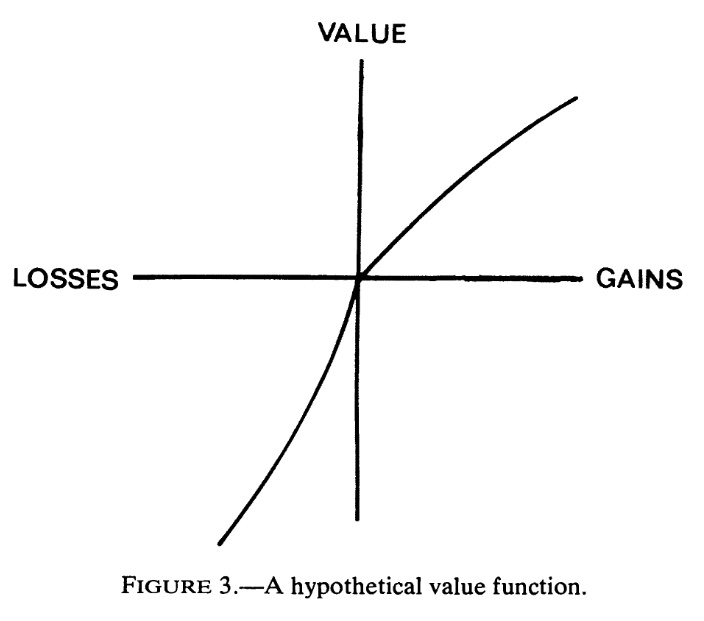
\includegraphics{prospect-theory/img/kahneman_and_tversky_1979_figure_3.jpg}

\hypertarget{probability-weighting}{%
\chapter{Probability weighting}\label{probability-weighting}}

In Expected Utility Theory, probabilities enter the expected utility
function linearly. That is, if an event is twice as likely as another
outcome it has double the weight.

Experimental observation confirms that we approximate linear
probabilities for intermediate probabilities. But, there is strong
evidence that we give overweight certain events (i.e.~when \(p\) = 1)
relative to near certain events (e.g.~when \(p\) = 0.99). This is
effectively the same as overweighting very low probability events.

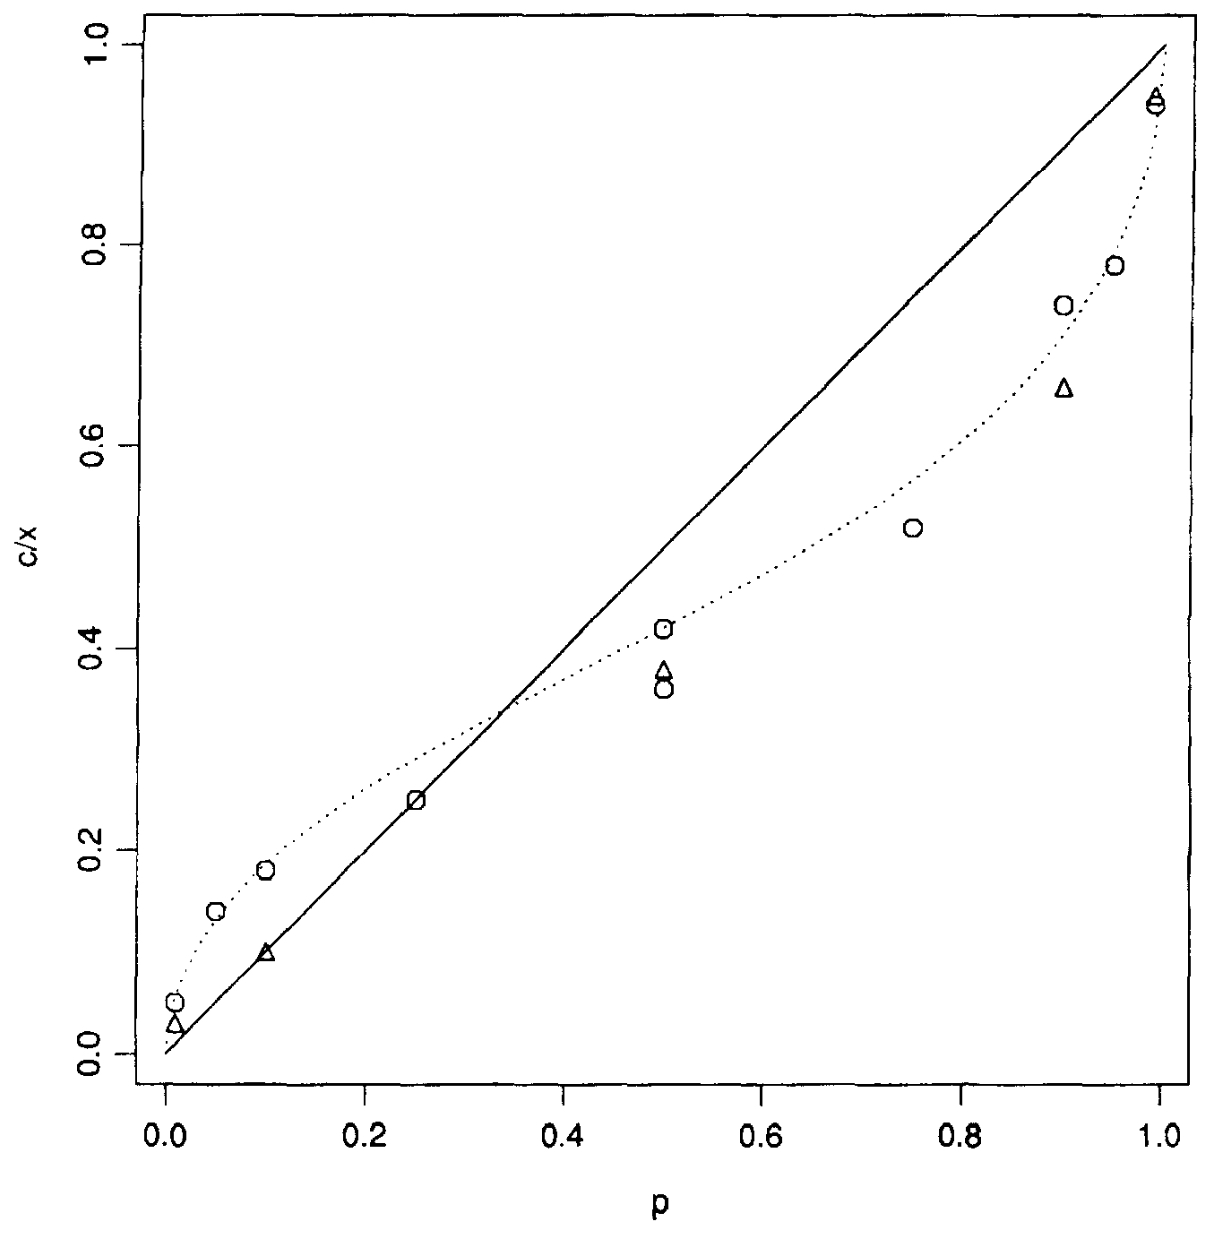
\includegraphics[width=0.6\textwidth,height=\textheight]{prospect-theory/img/tversky_and_kahneman_1992_figure_1.jpg}

Recall our discussion of the Allais Paradox in Section~\ref{sec-allais}.

\textbf{Choice 1}: Choose one of the following bets:

Bet A:

\begin{itemize}
\tightlist
\item
  \$2500 with probability: 33\%
\item
  \$2400 with probability: 66\%
\item
  \$0 with probability: 1\%
\end{itemize}

Bet B:

\begin{itemize}
\tightlist
\item
  \$2400 with probability: 100\%
\end{itemize}

\textbf{Choice 2}: Choose one of the following bets:

Bet C:

\begin{itemize}
\tightlist
\item
  \$2500 with probability: 33\%\\
\item
  \$0 with probability: 67\%
\end{itemize}

Bet D:

\begin{itemize}
\tightlist
\item
  \$2400 with probability: 34\%
\item
  \$0 with probability: 66\%
\end{itemize}

If you look at Bet B, this involves a certain outcome, which tennds to
be overweighted relative to near-certain events (the 99\% chance of
\$2400 or \$2500).

Kahneman (2011) calls the large psychological value of the change from 0
to 5\% (or some other small probability) the possibility effect. Very
unlikely but possible outcomes are given more weight than similar
increases in probability for events that are already possible. He calls
the large psychological value of the change to 100\% the certainty
effect. We will pay a lot more for certainty than near certainty.

\hypertarget{the-decision-weight}{%
\section{The decision weight}\label{the-decision-weight}}

Under expected utility theory, the utility of a prospect is a linear
expectation. Each possible outcome is weighted by its probability.

In Prospect Theory the decision maker does not weigh probabilities
linearly but instead attaches a decision weight \(\pi(p_i)\) to each
probability.

The new decision-weighting function reflects the empirical regularity we
discussed previously: people overweight certain events (i.e.~when \(p\)
= 1) relative to near certain events (e.g.~when \(p\) = 0.99) and
overweight very low probability events

\hypertarget{prospect-theory-implementation}{%
\chapter{Prospect theory
implementation}\label{prospect-theory-implementation}}

Under Prospect theory, people evaluate the utility of a prospect by two
phases: editing and evaluation.

\hypertarget{editing}{%
\section{Editing}\label{editing}}

Editing involves simplification of prospects for subsequent evaluation.

Kahneman and Tversky (1979) describes the editing phase as having four
main operations:

\begin{itemize}
\item
  Coding: People perceive outcomes as gains or losses relative to some
  neutral reference position. The reference point is may be the status
  quo or some other expectation of agent.
\item
  Combination: Prospects are simplified by combining probabilities for
  identical outcomes: (200, 0.25; 200, 0.25) will become (200, 0.50).
\item
  Segregation: Riskless components are segregated out from risky
  components. For example (300, 0.80; 200, 0.20) corresponds to a a sure
  gain of 200 and the risky gamble (100, 0.80).
\item
  Cancellation: Components that are shared by two prospects are ignored.
\end{itemize}

\hypertarget{evaluation}{%
\section{Evaluation}\label{evaluation}}

In the evaluation phase the prospects are evaluated and the option with
the highest value chosen.

The value of a prospect is made up of:

1. a decision weight applied to each probability \(\pi(p_i)\)

2. the subjective value of each outcome \(v(x_i)\)

These are applied through the following formula (often called the value
function):

\begin{align*}
V(X)&=\sum_{i=1}^n\pi(p_i)v(x_i)\\[6pt]
&=\pi(p_1)v(x_1)+\pi(p_2)v(x_2)+...+\pi(p_n)v(x_n)
\end{align*}

Where \(V(X)\) is the expected value of the outcomes from gamble \(X\).

The following diagrams illustrate the different shapes of the expected
utility function and the Prospect Theory value function.

The expected utility function has diminishing marginal utility as
utility increases. Utility is measured from a base reference point.

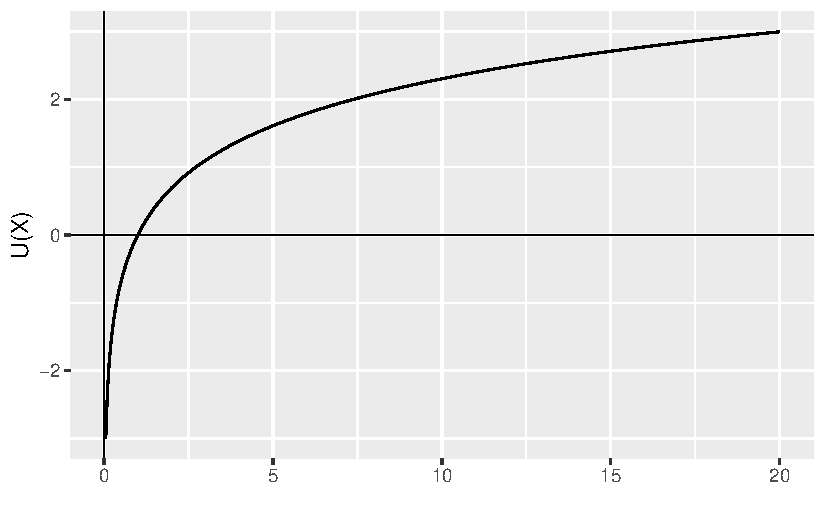
\includegraphics{prospect-theory/prospect-theory-implementation_files/figure-pdf/unnamed-chunk-1-1.pdf}

For the prospect theory function, you can see the kink at zero, with
losses weighted more heavily than gains, with gains and losses
determined relative to a reference point. There is diminishing
sensitivity to further changes in both directions

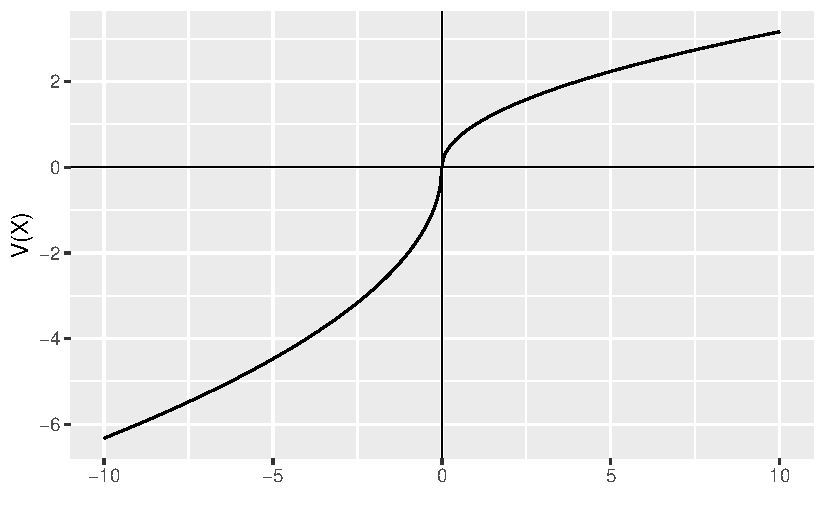
\includegraphics{prospect-theory/prospect-theory-implementation_files/figure-pdf/unnamed-chunk-2-1.pdf}

\hypertarget{fourfold-pattern-of-risk-attitudes}{%
\section{Fourfold pattern of risk
attitudes}\label{fourfold-pattern-of-risk-attitudes}}

Prospect theory results in a four-fold pattern of risk attitudes, as
shown in this table. For moderate to high probability gambles, the
reflection effect dominates and people are risk averse in the domain of
gains and risk seeking in the domain of losses.

But for low probability gambles, the probability weighting shifts the
decision calculus. The possibility of a gain is overweighted, making the
gamble attractive and inducing risk seeking behaviour. A similar effect
occurs for a low probability of loss, with the overweighted probability
making the potential loss less attractive, inducing risk averse
behaviour.

\begin{longtable}[]{@{}
  >{\raggedright\arraybackslash}p{(\columnwidth - 4\tabcolsep) * \real{0.5833}}
  >{\raggedright\arraybackslash}p{(\columnwidth - 4\tabcolsep) * \real{0.2083}}
  >{\raggedright\arraybackslash}p{(\columnwidth - 4\tabcolsep) * \real{0.2083}}@{}}
\toprule()
\begin{minipage}[b]{\linewidth}\raggedright
\end{minipage} & \begin{minipage}[b]{\linewidth}\raggedright
Gains
\end{minipage} & \begin{minipage}[b]{\linewidth}\raggedright
Losses
\end{minipage} \\
\midrule()
\endhead
\textbf{Medium to high probability} & Risk aversion & Risk seeking \\
\textbf{Low probability} (possibility effect) & Rick seeking & Risk
aversion \\
\bottomrule()
\end{longtable}

\hypertarget{prospect-theory-examples}{%
\chapter{Prospect Theory examples}\label{prospect-theory-examples}}

\hypertarget{insurance}{%
\section{Insurance}\label{insurance}}

The classical economic explanation for the purchase of insurance is
based on the risk aversion of consumers. Consumers are willing to buy
insurance with a negative expected value as the consumer prefers the
certainty of the premium payment to the risk of suffering an uninsured
loss. (The negative expected value is due to the insurer's profit and
administrative costs.)

Prospect theory provides an alternative explanation. The purchase of
insurance involves a certain loss (the premium) or a gamble involving
the possibility of either a large loss or the status quo. As prospect
theory has people as risk seeking in the loss domain, we would not
expect them to purchase insurance.

However, under prospect theory people also overweight small
probabilities. This overweighting of small probabilities can make the
purchase of insurance attractive even though it is in the loss domain.
This combination of the loss domain but small probabilities is the
bottom-right quadrant of the fourfold pattern to risk attitudes
generated by prospect theory.

The following numerical example is an illustration.

An agent is considering insurance against bushfire for its \$1,000,000
house. The house has a 1 in 1000 chance of burning down. An insurer is
willing to offer full coverage for \$1100. (Note: \$1000 is the
actuarially fair price, the additional \$100 might represent profit or
administrative costs.)

\hypertarget{expected-value-1}{%
\subsection{Expected value}\label{expected-value-1}}

Would an expected value maximiser or risk neutral person purchase the
insurance?

\begin{align*}
E[\text{purchase}]&=-\text{premium} \\
&=-\$1,100
\end{align*}

The expected value of purchasing insurance is the guaranteed loss of the
premium.

\begin{align*}
E[\text{don't}]&=P_{\text{burn}}\times -value_{\text{house}} \\
&=-0.001\times 1000000 \\
&=-\$1000
\end{align*}

The expected value of purchasing insurance is \$100 less than the
expected value of risking the house burning down. A risk neutral agent
(who maximises expected value) would not purchase this insurance.

\hypertarget{expected-utility}{%
\subsection{Expected utility}\label{expected-utility}}

Would a risk averse agent purchase the insurance? Suppose they have a
logarithmic utility function (\(U(x)=ln(x)\)) and they have \$10,000 in
cash in addition to their house, giving them wealth (\(W\)) of
\$1,010,000.

\begin{align*}
E[U(\text{purchase})]&=ln(W-premium) \\
&=ln(1,008,900) \\
&=13.8244 \\
\\
E[U(\text{don't})]&=0.999\times ln(W)+0.001\times ln(W-value_{\text{house}}) \\
&=0.999\times ln(1,010,000)+0.001\times ln(10,000) \\
&=13.8208
\end{align*}

The expected utility of purchasing insurance is greater than the
expected utility from not purchasing insurance. This agent will insure
against the fire despite it being actuarially unfair.

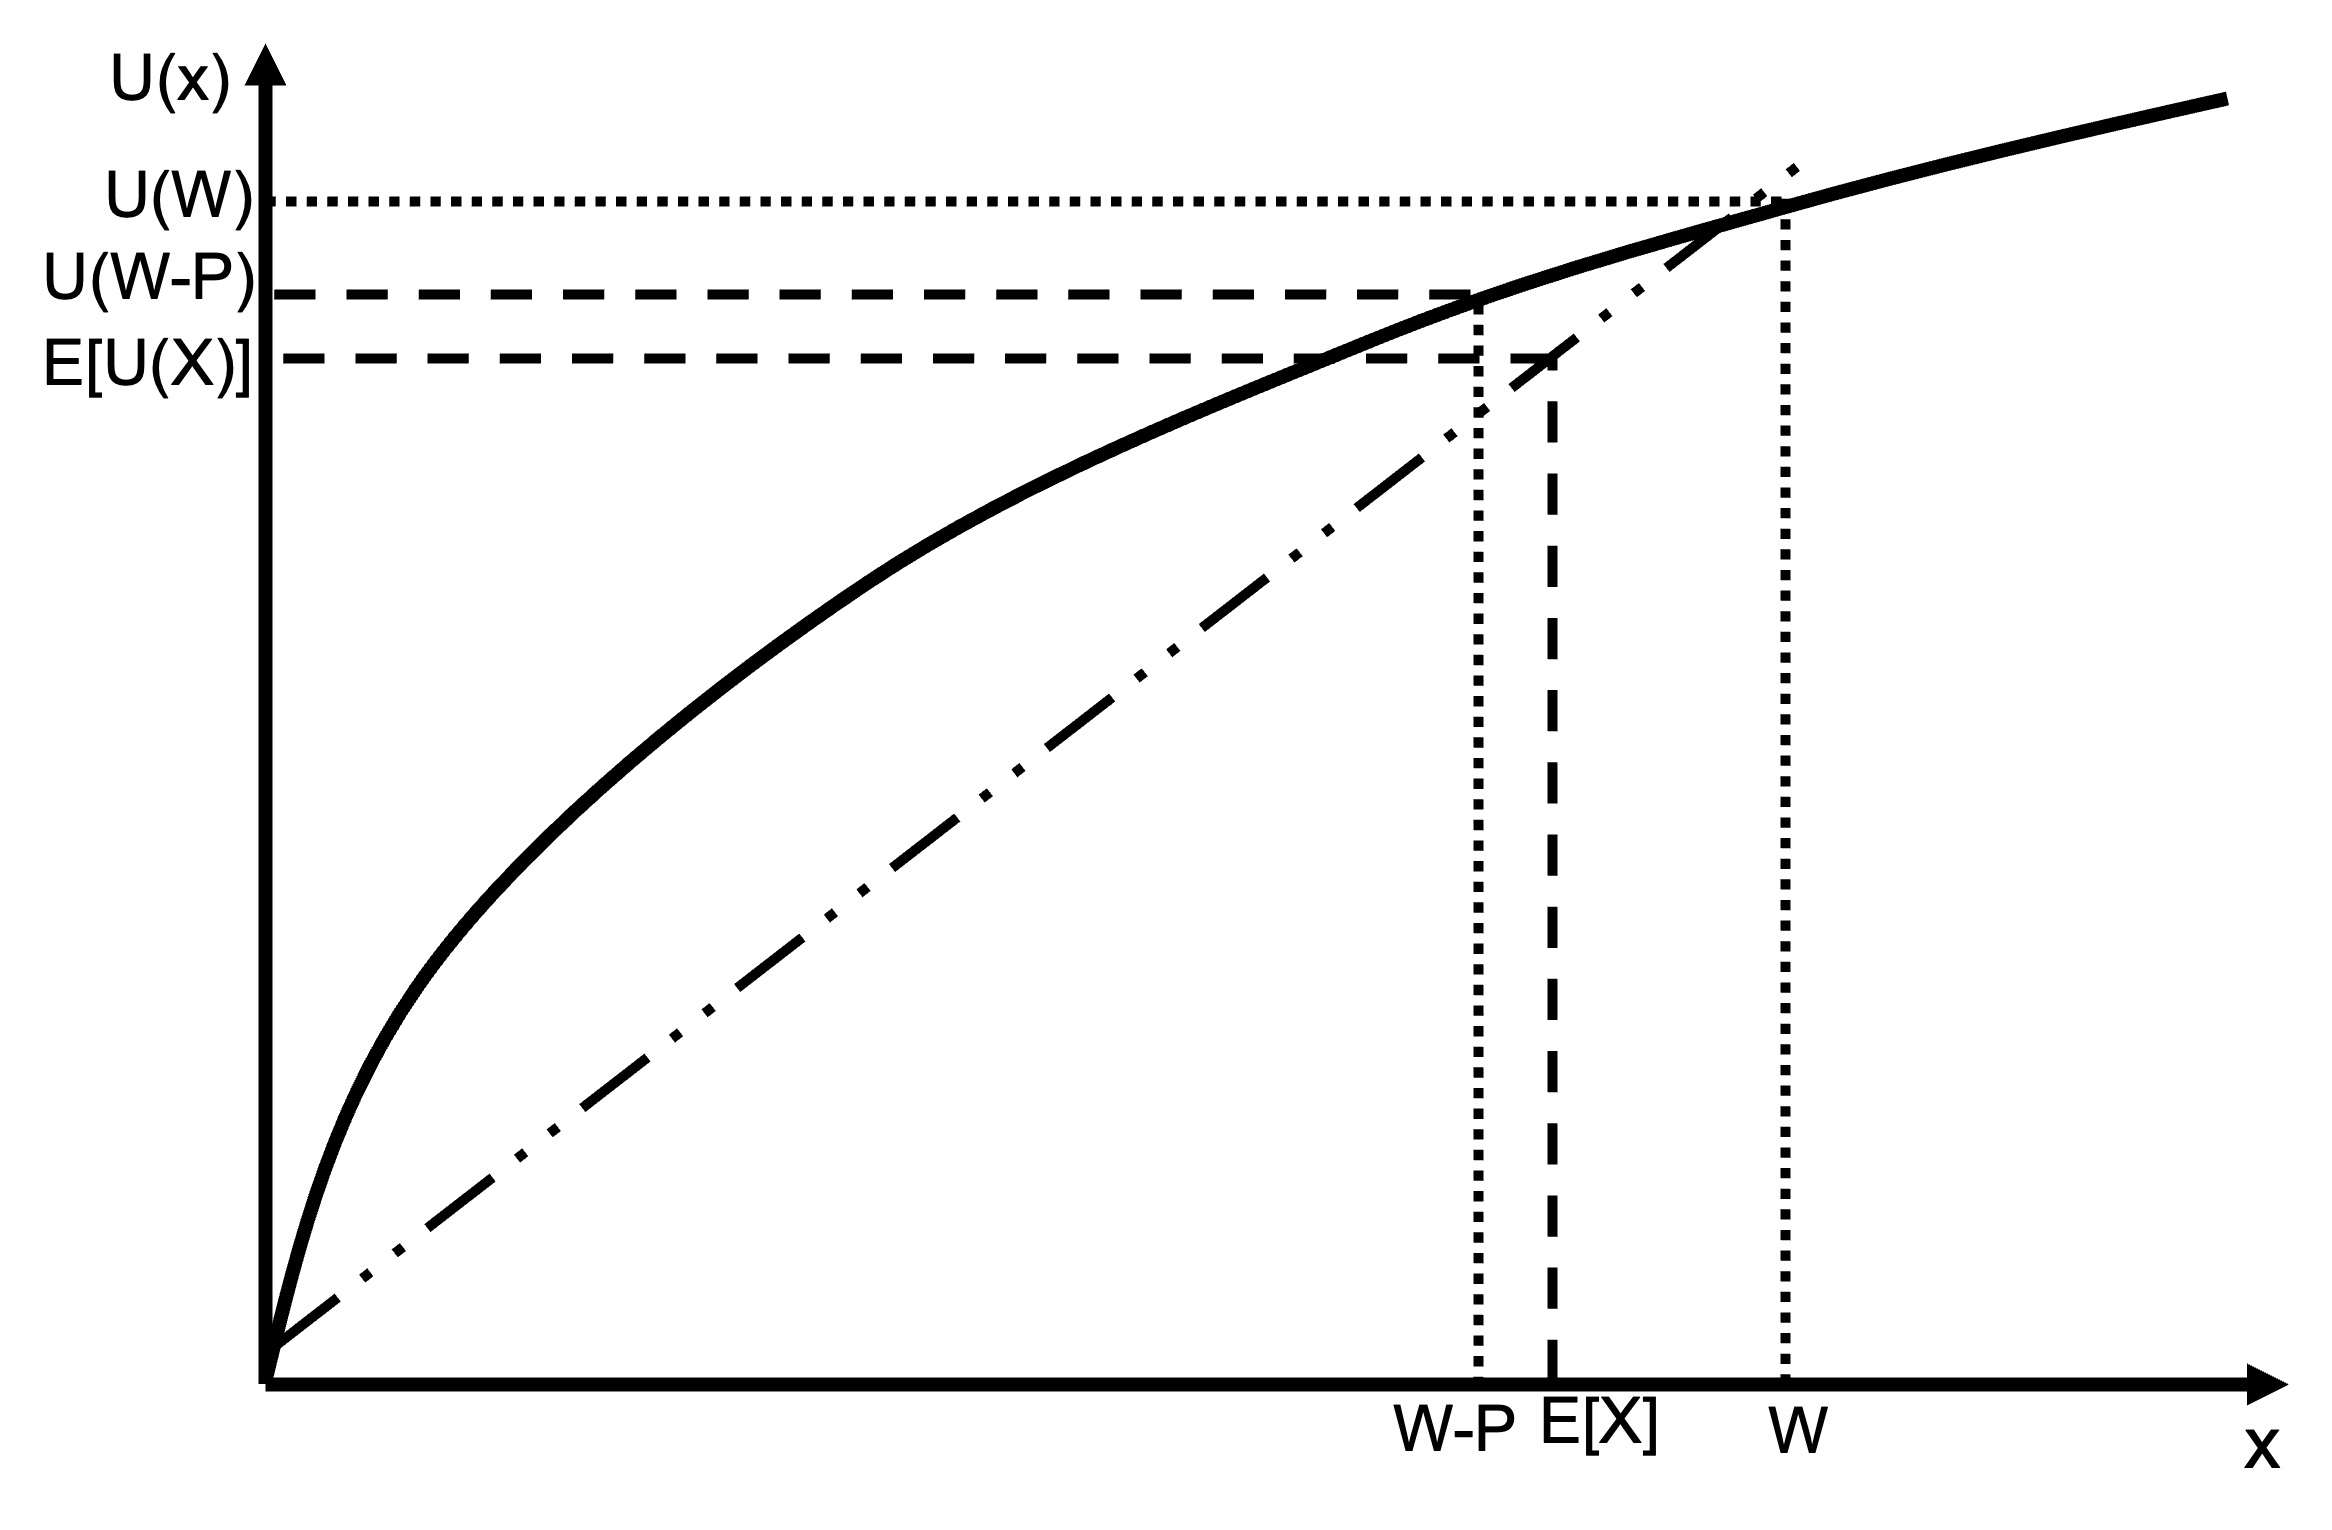
\includegraphics{prospect-theory/img/expected-utility.jpg}

\hypertarget{the-reflection-effect-1}{%
\subsection{The reflection effect}\label{the-reflection-effect-1}}

Consider an agent who is risk seeking in the domain of losses but
weights probability linearly. Their value function is:

\[
v(x)=\left\{\begin{matrix}
x^{0.8} \qquad &\textrm{where} \space x \geq 0\\
-2(-x)^{0.8} \quad &\textrm{where} \space x < 0 
\end{matrix}\right.
\]

Where \(x\) is the realised outcome relative to the reference point.

Determination of the reference point can be arbitrary. What if you pay
insurance every year? Could the reference point then be wealth minus the
insurance payment (meaning the insurance payment is in the gain domain)?

Taking the reference point as current wealth, would this agent purchase
the insurance?

\begin{align*}
V(purchase)&=v(-1,100) \\
&=-(1,100)^{0.8} \\
&=-271.1 \\
\\
V(don't)&=0.999\times (0)+0.001\times v(-1,000,000) \\
&=0.999\times 0-0.001\times (1,000,000)^{0.8} \\
&=-63.1
\end{align*}

As \(V(purchase)<V(don't)\), the agent does not purchase insurance. The
diminishing feeling of loss leads to them weigh the certain loss of the
premium relatively more heavily than the chance of losing the value of
their house.

Including loss aversion in the value function does not change the
decision as all possible outcomes are in the loss domain.

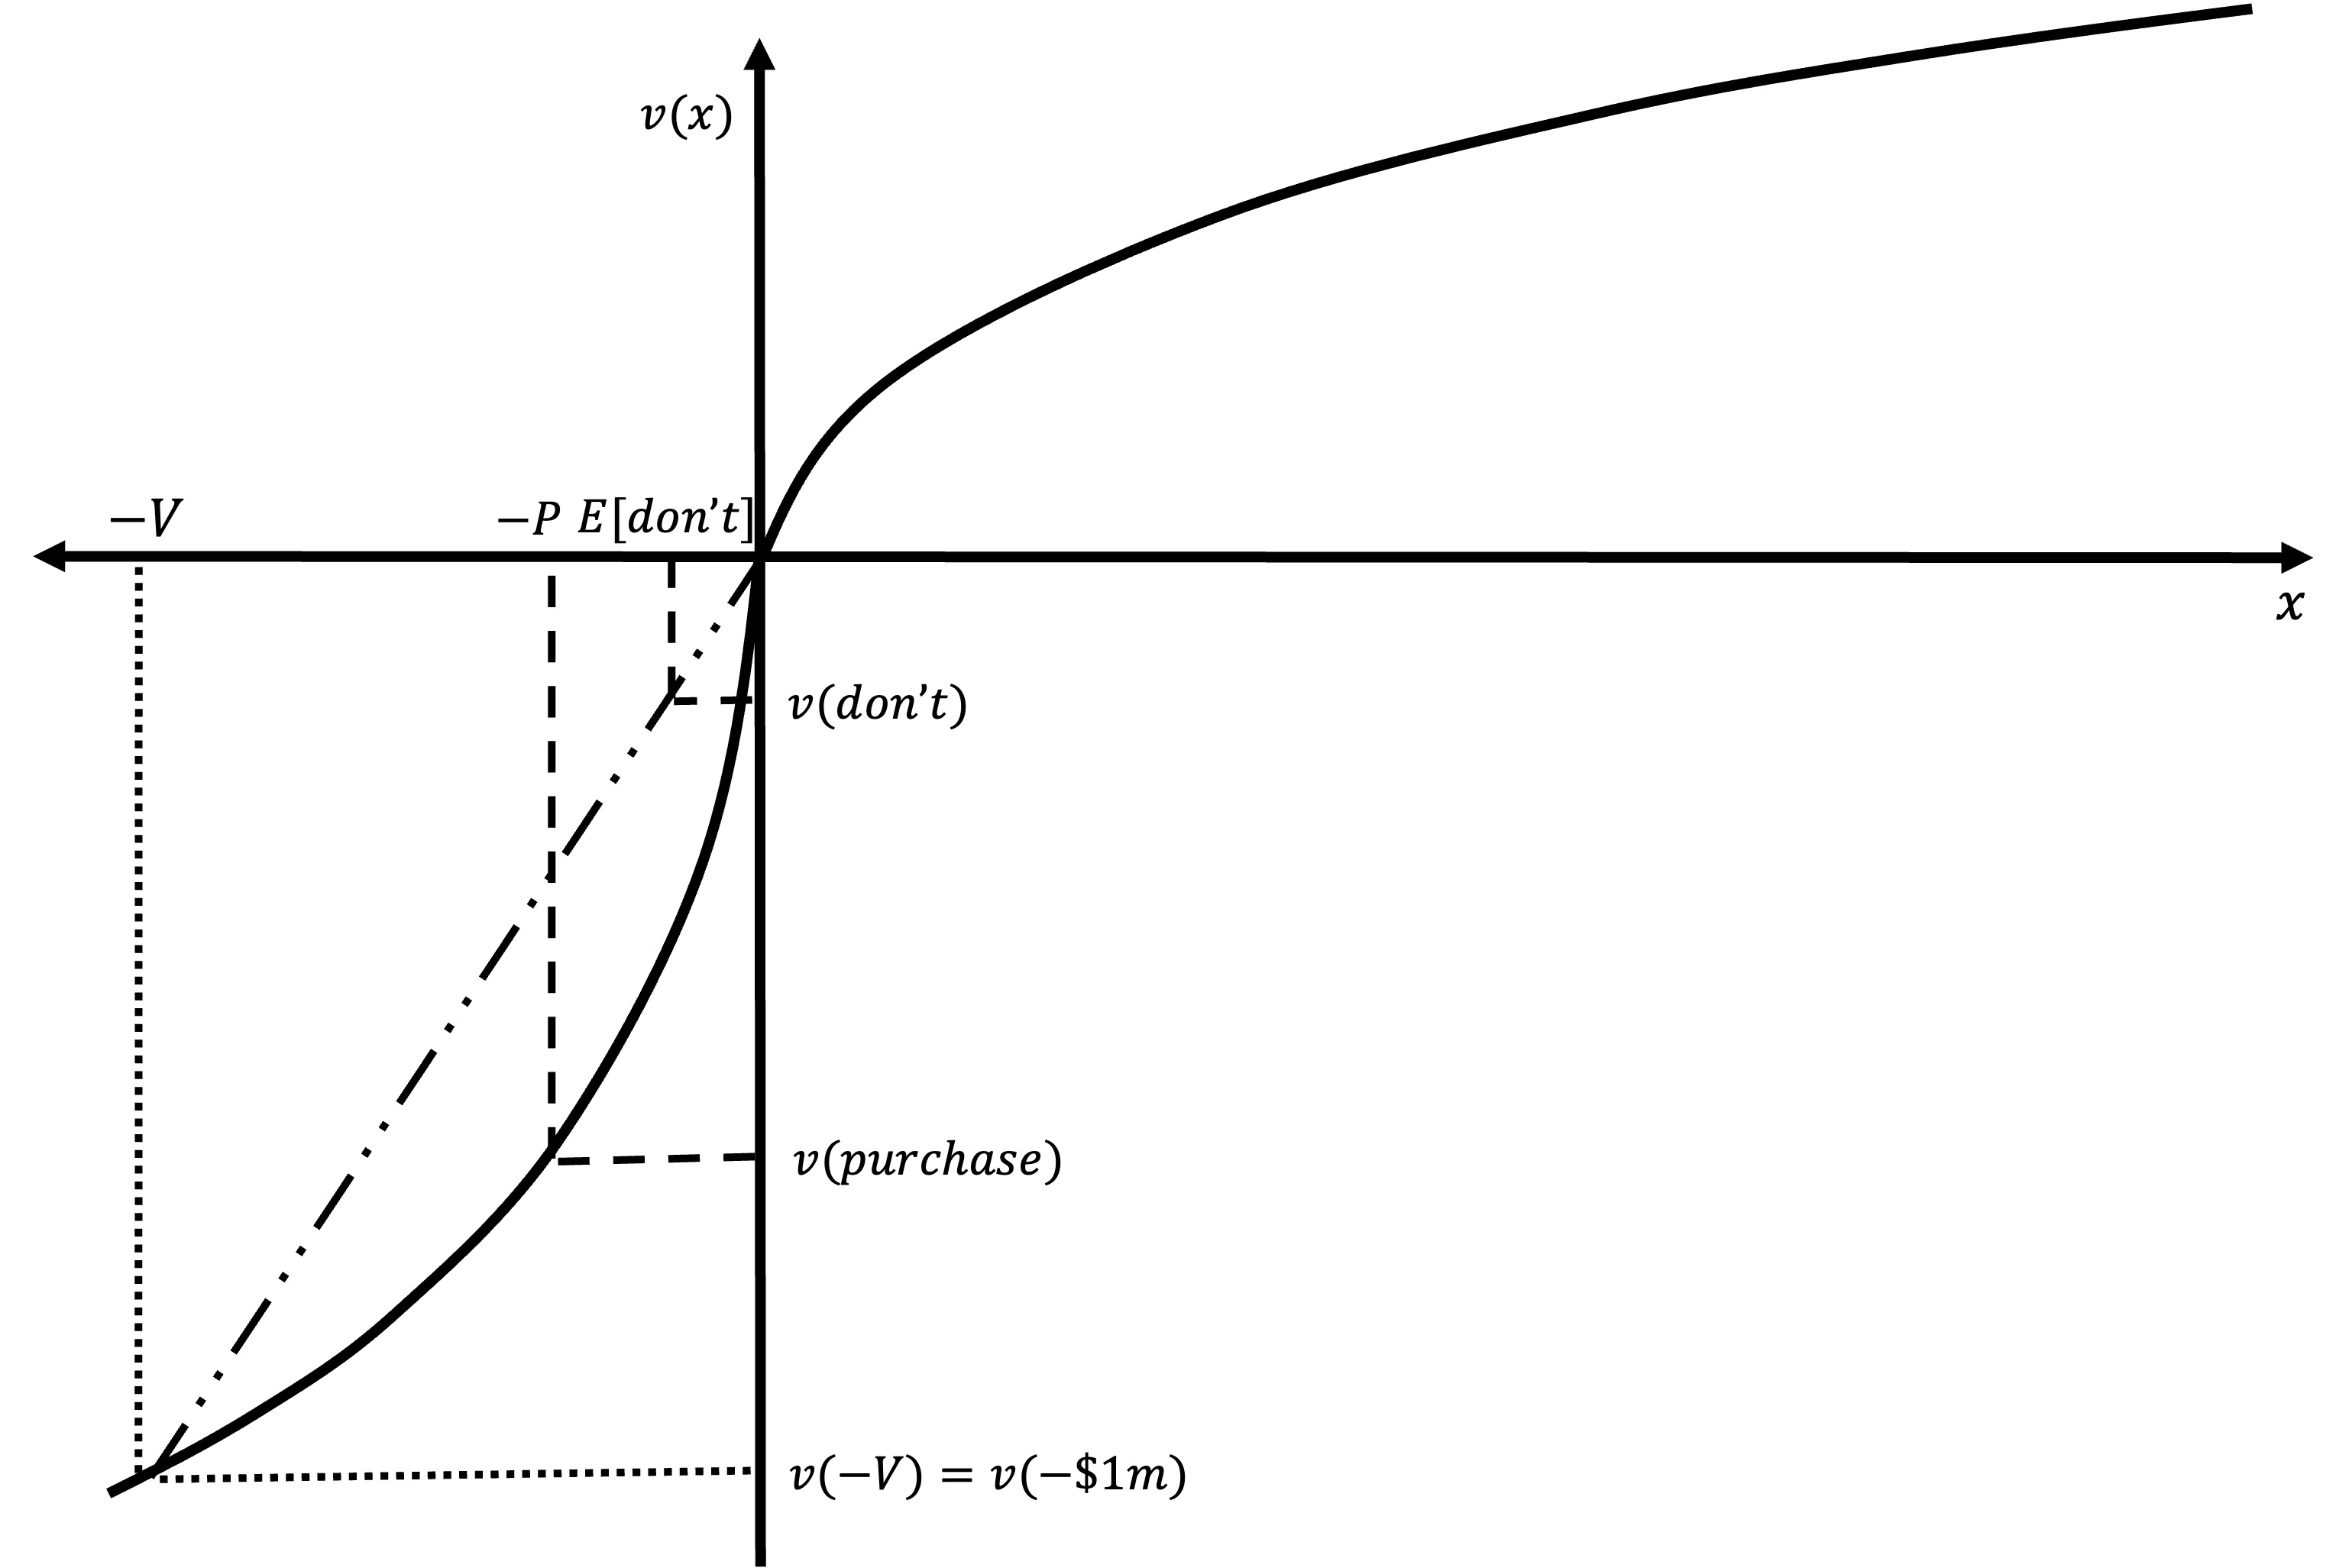
\includegraphics{prospect-theory/img/reflection-effect.jpg}

\hypertarget{probability-weighting-1}{%
\subsection{Probability weighting}\label{probability-weighting-1}}

Would a person who is risk seeking in the domain of losses (i.e.~the
value function with reflection effect above) and applies the decision
weights described below purchase the insurance?

They apply decision weights as per the following table:

\begin{longtable}[]{@{}
  >{\raggedright\arraybackslash}p{(\columnwidth - 18\tabcolsep) * \real{0.1000}}
  >{\raggedright\arraybackslash}p{(\columnwidth - 18\tabcolsep) * \real{0.1000}}
  >{\raggedright\arraybackslash}p{(\columnwidth - 18\tabcolsep) * \real{0.1000}}
  >{\raggedright\arraybackslash}p{(\columnwidth - 18\tabcolsep) * \real{0.1000}}
  >{\raggedright\arraybackslash}p{(\columnwidth - 18\tabcolsep) * \real{0.1000}}
  >{\raggedright\arraybackslash}p{(\columnwidth - 18\tabcolsep) * \real{0.1000}}
  >{\raggedright\arraybackslash}p{(\columnwidth - 18\tabcolsep) * \real{0.1000}}
  >{\raggedright\arraybackslash}p{(\columnwidth - 18\tabcolsep) * \real{0.1000}}
  >{\raggedright\arraybackslash}p{(\columnwidth - 18\tabcolsep) * \real{0.1000}}
  >{\raggedright\arraybackslash}p{(\columnwidth - 18\tabcolsep) * \real{0.1000}}@{}}
\toprule()
\endhead
\textbf{Probability} & 0.001 & 0.01 & 0.1 & 0.25 & 0.5 & 0.75 & 0.9 &
0.99 & 0.999 \\
\textbf{Weight} & 0.01 & 0.05 & 0.15 & 0.3 & 0.5 & 0.7 & 0.85 & 0.95 &
0.99 \\
\bottomrule()
\end{longtable}

\begin{align*}
V(purchase)&=v(-1,100) \\
&=-(1,100)^{0.8} \\
&=-271 \\
\\
V(don't)&=\sum_{i=1}^n \pi(p_i)v(x_i) \\
&=\pi(0.999)\times v(0)+\pi(0.001)\times v(-1,000,000) \\
&=0.99\times 0-0.01\times (1,000,000)^{0.8} \\
&=-631
\end{align*}

Although the diminishing feeling of loss leads to them weigh the certain
loss of the premium relatively more heavily than the chance of losing
the value of their house, the overweighting of the probability of fire
leads them to purchase insurance. Again, if we had included loss
aversion it would not have changed the decision as all possible outcomes
are in the loss domain.

\hypertarget{a-5050-gamble-1}{%
\section{A 50:50 gamble}\label{a-5050-gamble-1}}

Suppose an agent has the following reference-dependent utility function:

\[
v(x)=\left\{\begin{matrix}
x^{1/2} \qquad &\textrm{where} \space x \geq 0\\
-2(-x)^{1/2} \quad &\textrm{where} \space x < 0 
\end{matrix}\right.
\]

Where \(x\) is the realised outcome relative to the reference point.

Assume that the agent's reference point is the status quo and the agent
is offered the gamble A:

\[(\$110, 0.5; −\$100, 0.5)\]

\hypertarget{accept-or-reject}{%
\subsection{Accept or reject}\label{accept-or-reject}}

Will they want to play this gamble?

The utility from the gamble is:

\begin{align*}
V(A)&=0.5v(110)+0.5v(-100) \\
&=0.5\times (110)^{0.5}-0.5\times 2\times (100)^{0.5} \\
&=-4.76
\end{align*}

They will not want to play this gamble as it has a negative value for
the agent. They could receive value of 0 by simply not playing.

The reason for this negative value is that the agent is loss averse. The
loss of \$100 is given twice the weight of an equivalent gain.

\hypertarget{accept-or-reject-after-loss}{%
\subsection{Accept or reject after
loss}\label{accept-or-reject-after-loss}}

Suppose the agent loses their wallet containing \$100. They feel bad
about it and perceive it as a loss. Their reference point is unchanged
at the original status quo, but the amount of money they have any after
any outcome is \$100 less than otherwise. Would they be willing to take
gamble A now?

After losing \$100 but not changing their reference point, they have two
possible outcomes relative to their reference point: a gain of \$10
(winning \$110 minus the lost money in the wallet) and a loss of \$200
(losing \$100 and also losing their wallet).

\begin{align*}
V(A)&=0.5v(110-100)-0.5v(-100-100) \\
&=0.5\times (10)^{0.5}-0.5\times 2\times (200)^{0.5} \\
&=-12.56
\end{align*}

The utility of not playing the gamble involves remaining with a loss of
\$100:

\begin{align*}
V(\neg A)&=v(-100) \\
&=-2\times (100)^{0.5} \\
&=-20
\end{align*}

They will now want to play the gamble as it has a greater value than
staying with their current loss. The reason the gamble becomes
attractive is because it gives an opportunity to recover the loss. The
agent is risk seeking over the loss domain. (They would even accept a
50:50 gamble to win \$100, lose \$100 with an expected value of zero.)

\hypertarget{accept-or-reject-after-adapt-to-loss}{%
\subsection{Accept or reject after adapt to
loss}\label{accept-or-reject-after-adapt-to-loss}}

The agent has now adapted to their loss of \$100. The new reference
point is the new wealth level incorporating the loss wallet. Would they
take gamble A now?

We are now back to an identical situation as in Question 1. They will
not want to partake in the gamble.

\hypertarget{accept-or-reject-after-win}{%
\section{Accept or reject after win}\label{accept-or-reject-after-win}}

The agent wins \$10,000 at the casino. They feel good about their win,
so their reference point remains at their wealth excluding the win.
Would they take gamble A now?

With the additional \$10,000, the value from the gamble is now:

\begin{align*}
V(A)&=0.5v(10000+110)+0.5v(10000-100) \\[6pt]
&=0.5\times (10110)^{0.5}+0.5\times (9900)^{0.5} \\[6pt]
&=100.02
\end{align*}

The value of not playing the gamble is:

\begin{align*}
V(\neg A)&=v(10000) \\[6pt]
&=(10000)^{0.5} \\[6pt]
&=100
\end{align*}

The gamble is now attractive. They are less risk averse at a higher
wealth, and the gamble is entirely in the gain domain, meaning that loss
aversion does not affect the decision.

\hypertarget{a-6040-gamble-1}{%
\section{A 60:40 gamble}\label{a-6040-gamble-1}}

Paddy makes decisions in accordance with prospect theory, has wealth
\$300 and value function:

\[
v(x)=\left\{\begin{matrix}
x^{\frac{1}{2}} \quad &\textrm{where} \quad x \geq 0 \\
-2(-x)^{\frac{1}{2}} \quad &\textrm{where} \quad x < 0 
\end{matrix}\right.
\]

Penny and Paddy are offered the following bet A:

\begin{itemize}
\tightlist
\item
  a 60\% probability to win \$150
\item
  a 40\% probability to lose \$100.
\end{itemize}

\hypertarget{accept-or-reject-1}{%
\subsection{Accept or reject}\label{accept-or-reject-1}}

Does Paddy accept bet A?

Paddy compares the value of taking versus not taking the bet:

\begin{align*}
V(\text{A})&=p_1v(x_1)+p_2v(x_2) \\
&=0.6\times (150)^{\frac{1}{2}}-0.4\times 2\times (100)^{\frac{1}{2}} \\
&=-0.652
\end{align*}

The value of not taking the bet is zero. Paddy would have no change from
his reference point.

As \(V(A)<V(0)=0\), Paddy rejects the bet.

\hypertarget{accept-or-reject-after-loss-1}{%
\subsection{Accept or reject after
loss}\label{accept-or-reject-after-loss-1}}

Following some bad economic news, Paddy's wealth declines to \$150.
Paddy cannot get over the loss, so his reference point remains his
former wealth of \$300.

Paddy is offered bet A again. Does Paddy accept the bet?

As Paddy is now in the loss domain, the two potential outcomes from the
bet are a gain of \$0 and a loss of \$250. His alternative is remaining
at a point \$150 below his reference point (\(L\)).

Paddy compares the value of taking versus not taking the bet:

\begin{align*}
V(\text{A})&=p_1v(x_1)+p_2v(x_2) \\
&=0.6\times (-150+150)^{\frac{1}{2}}-0.4\times 2\times (150+100)^{\frac{1}{2}} \\
&=-12.649 \\
\\
V(\text{L})&=v(L) \\
&=-2\times (150)^{\frac{1}{2}} \\
&=-24.495
\end{align*}

As \(V(A)>V(L)\), Paddy accepts the bet.

\hypertarget{graphing-the-decision}{%
\subsection{Graphing the decision}\label{graphing-the-decision}}

For the bet above, draw diagrams showing Paddy's value function, the
bets and the value of the bets. Explain how the diagram(s) show whether
Paddy accepts or rejects the bet.

First offer: Paddy rejects the bet as \(V(A)\) is less than the
\(V(0)=0\) Paddy could get by simply rejecting the bet. This is caused
by both Paddy's loss aversion and his diminishing sensitivity in the
gain domain, which has larger effect that the diminishing sensitivity in
the loss domain due to the larger magnitude of the potential gain.

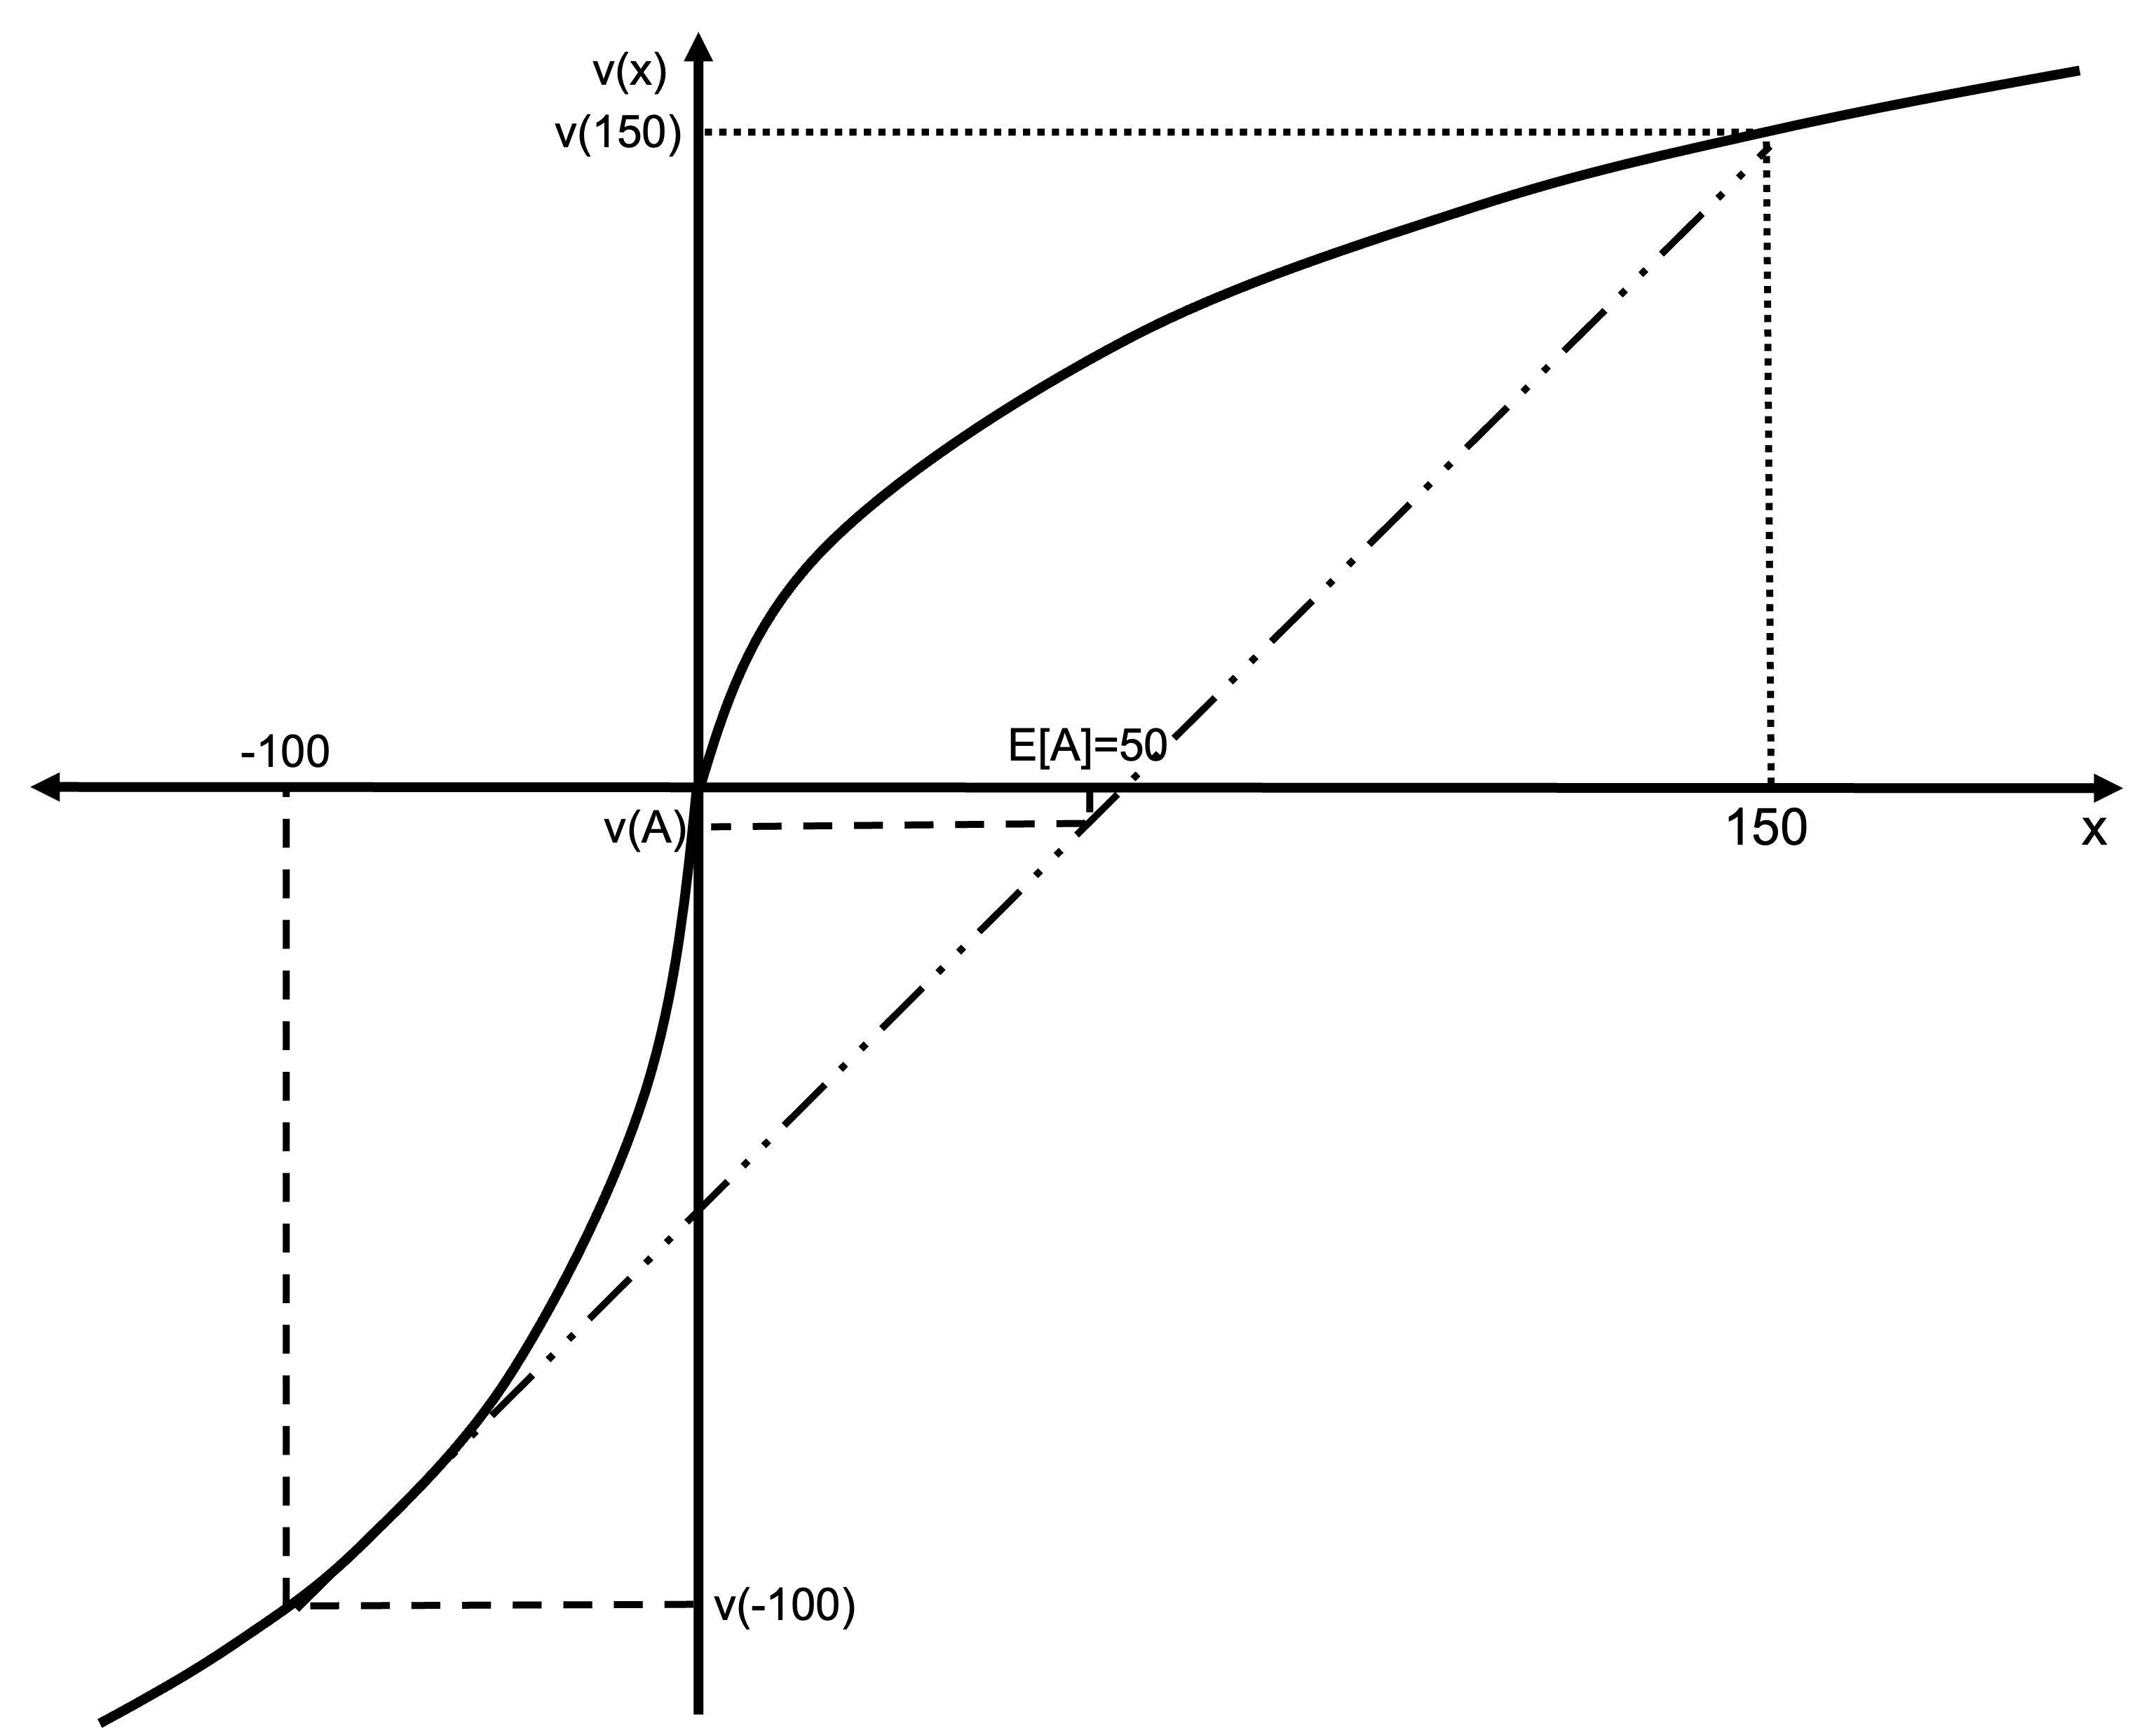
\includegraphics[width=0.8\textwidth,height=\textheight]{prospect-theory/img/paddy-1.jpg}

Second offer: Paddy accepts the bet as \(V(A)\) is greater than the
value of the certain loss of \$150. He is risk seeking in the loss
domain, so finds the positive expected value bet attractive.

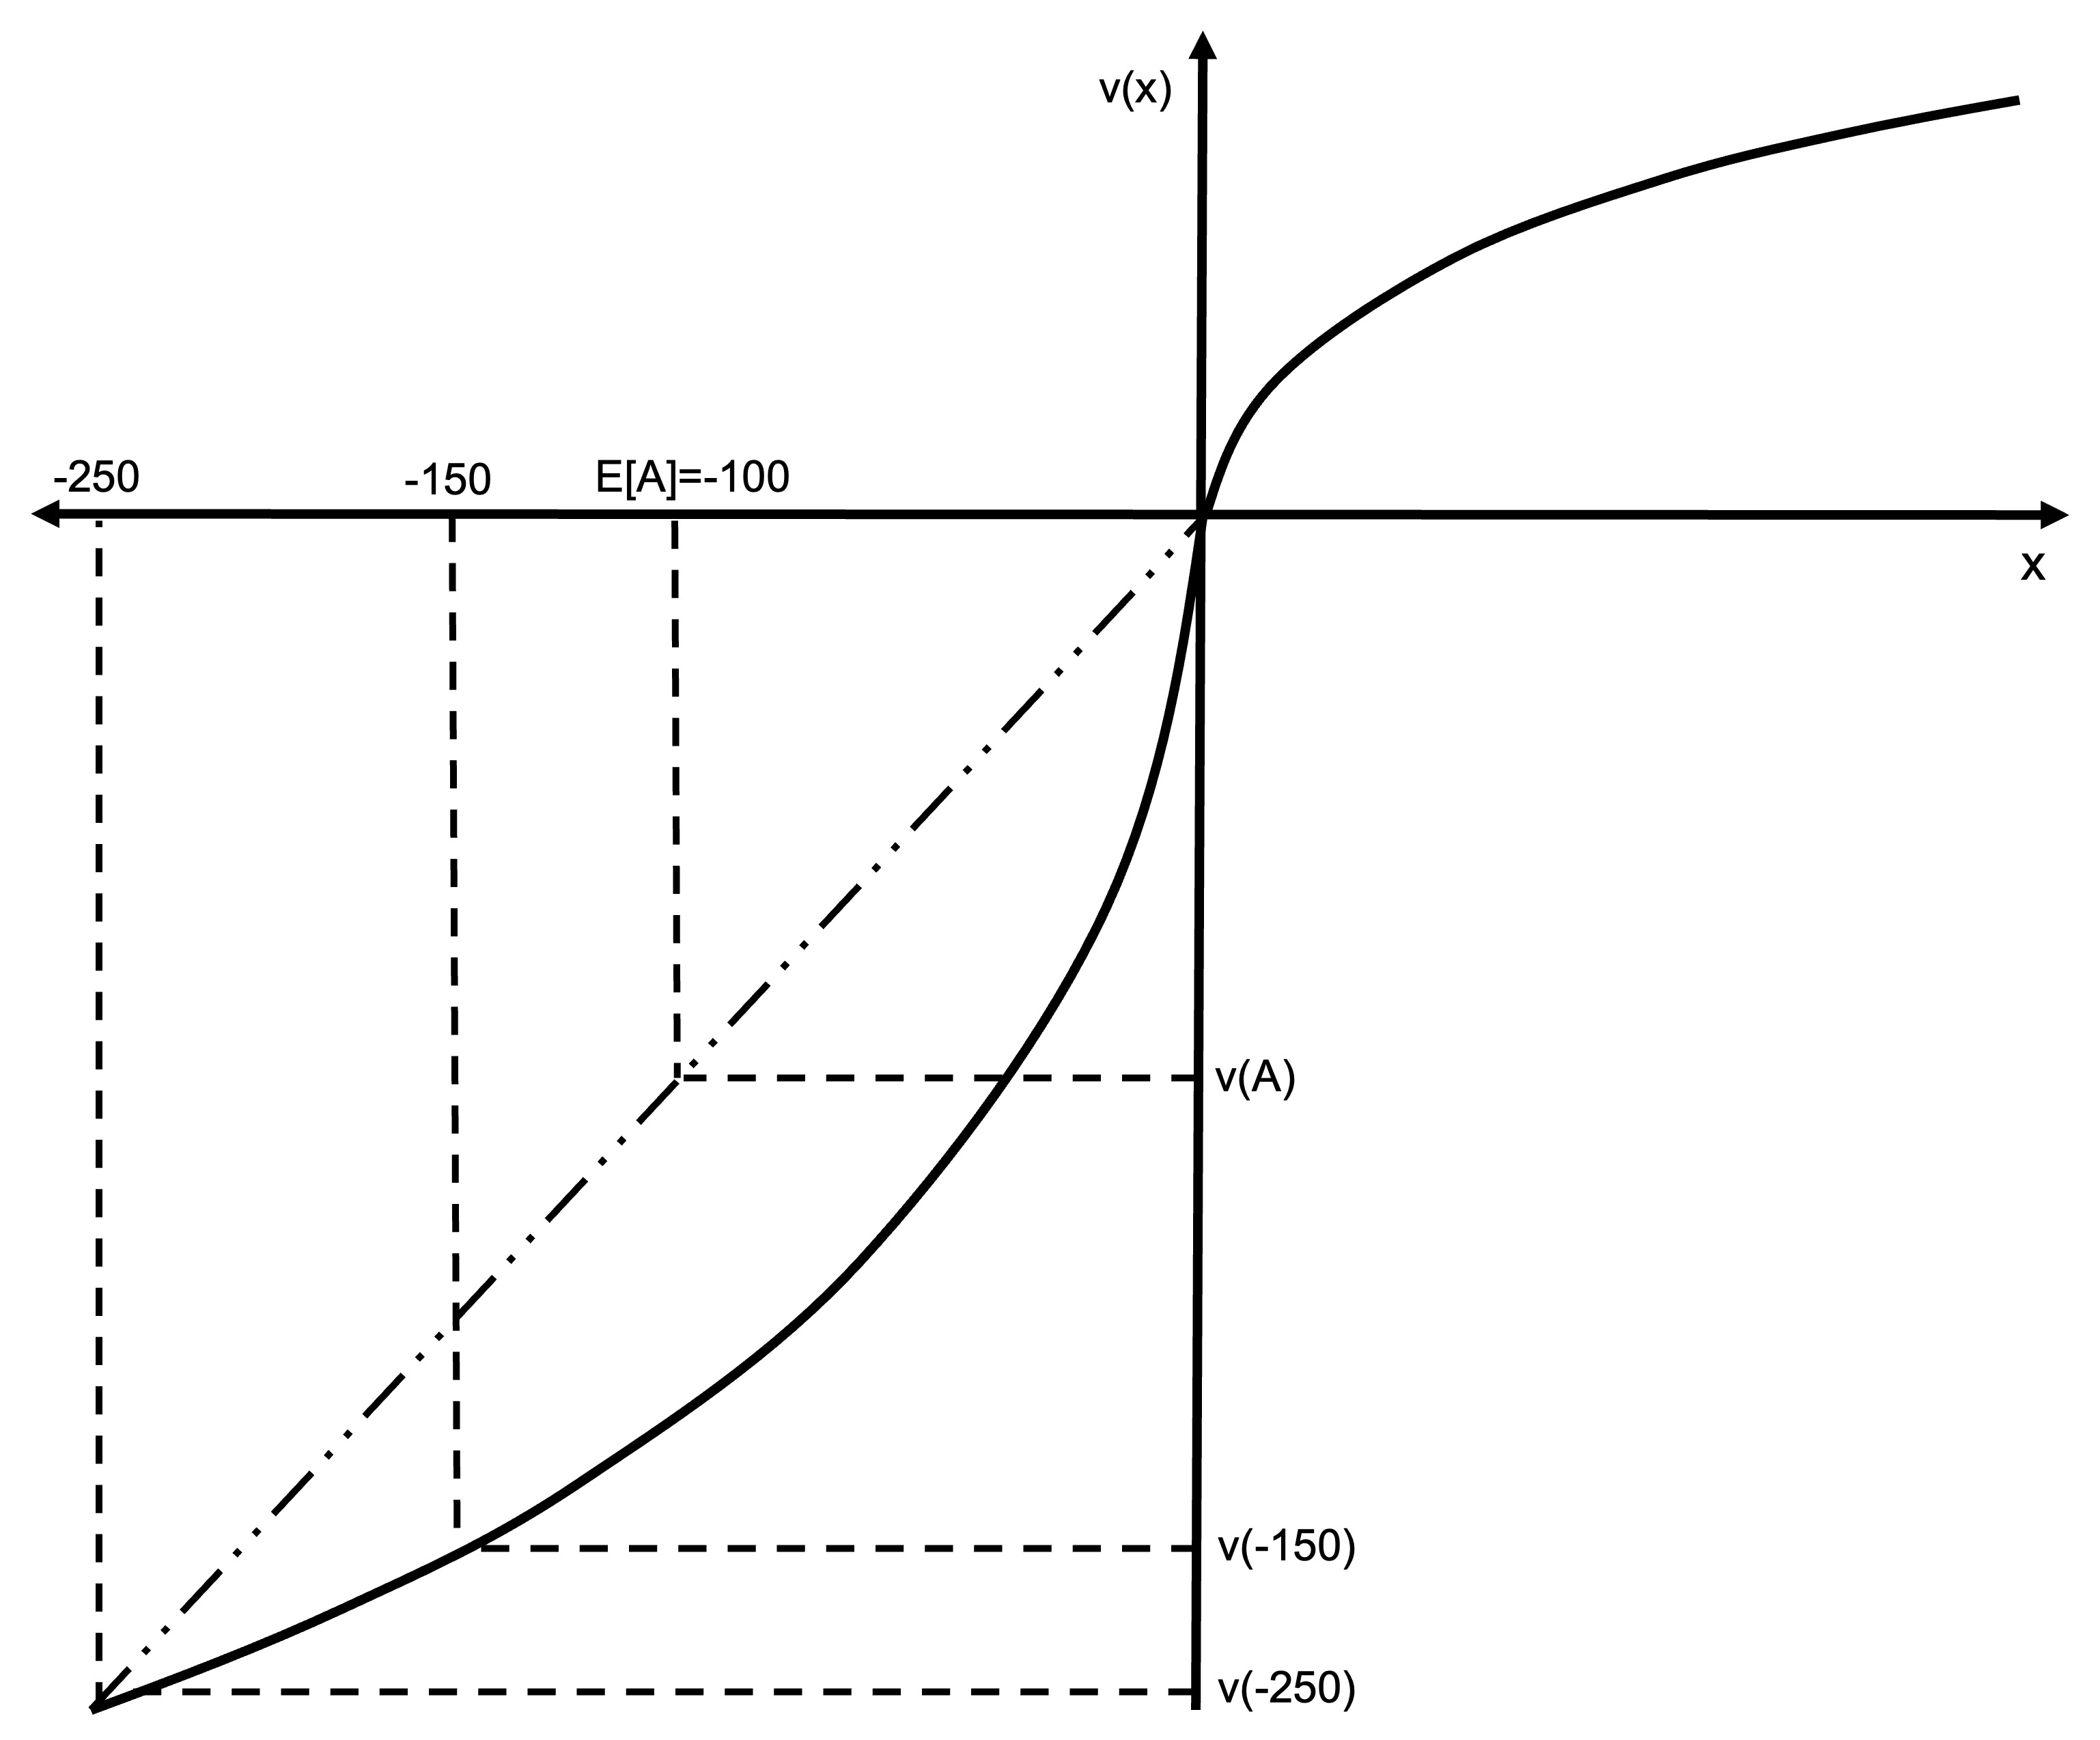
\includegraphics[width=0.8\textwidth,height=\textheight]{prospect-theory/img/paddy-2.jpg}

\hypertarget{prospect-theory-applications}{%
\chapter{Prospect theory
applications}\label{prospect-theory-applications}}

\hypertarget{taxi-drivers-on-rainy-days}{%
\section{Taxi drivers on rainy days}\label{taxi-drivers-on-rainy-days}}

Camerer et al.~(1997) studied the labour supply of New York City taxi
drivers.

The taxi drivers in the study rent a cab for a 12-hour period for a
fixed fee, plus petrol. Within the 12-hours, a driver can choose how
long they keep the taxi out.

For many reasons, such as weather, subway breakdowns, day of the week
and conferences, a taxi driver's effective wage can vary. When they are
busier, they have a higher effective wage (that is, more fares).

Camerer et al.~found that:

\begin{itemize}
\tightlist
\item
  The wage elasticity of drivers - that is, how their hours of driving
  respond to changes in their effective wages - was negative in two of
  the three samples. That is, drivers drove less when their effective
  wages were higher.
\item
  For inexperienced drivers, elasticities were negative in all three
  samples and significantly greater in magnitude than that for
  experienced drivers.
\end{itemize}

Camerer et al.~argue that this result is because taxi drivers have a
one-day time horizon for decision making, whereby they have an earnings
target beyond which they derive little additional utility. This leads
them to work until they reach their target, which they reach more
quickly on days with a higher wage.

\begin{itemize}
\tightlist
\item
  People have a tendency to engage in ``narrow bracketing'' when they
  make decisions, isolating them as single decisions (how much should I
  work today?) rather than thinking about them as a stream (how much
  should I work each day this week?)
\item
  Aversion to falling below the reference point is consistent with loss
  aversion, with a result below the reference point causing stronger
  feelings than a result a similar amount above the reference point.
\end{itemize}

There have been numerous follow-up studies of taxi-drivers:

\begin{itemize}
\item
  Farber (2005) studied New York cabdrivers and found that the decision
  to stop work was primarily a function of how many hours had been
  worked up to that point in the day. He identified the difference
  between his and Camerer et al.'s result as being due to different
  empirical methods and measurement problems with the Camerer et
  al.~data.
\item
  Farber (2008) found that a model of labour supply with
  reference-dependent targets has a better fit than a standard
  neoclassical model, but that there was substantial variation
  day-to-day in any given driver's reference income level and that most
  shift ends before that reference income is reached.
\item
  Farber (2015) used a much larger dataset on New York taxi driver
  behaviour and found that, as standard economic theory would predict,
  taxi drivers drive more when they can earn more. Farber also found
  that drivers did not earn more when it was raining.
\item
  Martin (2017) examined taxi driver labour supply incorporating the
  S-shaped reference dependence of Prospect Theory (the reflection
  effect with risk seeking behaviour in the loss domain and risk
  aversion in the gain domain. Martin found evidence that taxi driver
  behaviour was consistent with this fully form of Prospect Theory. He
  differentiated from the other papers on the basis that they considered
  a narrower version of reference dependence focusing on loss aversion
  only.
\end{itemize}

\hypertarget{the-disposition-effect}{%
\section{The disposition effect}\label{the-disposition-effect}}

The disposition effect is the tendency for investors to sell stocks that
are in the gain domain relative to the purchase price and to hold stocks
that are in the loss domain (Shefrin and Statman (1985)).

While tax implications or portfolio rebalancing are both potential
explanations for asymmetric behaviour relating to the sale of stocks,
these factors have been shown to be insufficient to explain the observed
behaviour.

Most behavioural explanations have turned to prospect theory.

For example, Shefrin and Statman (1985) argued that the disposition
effect is driven by the reflection effect, whereby investors are risk
seeking in the loss domain and risk averse in the gain domain. To
demonstrate how it works, they present the following scenario:

\begin{quote}
{[}C{]}onsider an investor who purchased a stock one month ago for \$50
and who finds that the stock is now selling at \$40. The investor must
now decide whether to realize the loss or hold the stock for one more
period. To simplify the discussion, assume that there are no taxes or
transaction costs. In addition, suppose that one of two equiprobable
outcomes will emerge during the coming period: either the stock will
increase in price by \$10 or decrease in price by \$10. According to
prospect theory, our investor frames his choice as a choice between the
following two lotteries:

A. Sell the stock now, thereby realizing what had been a \$10 ``paper
loss''.

B. Hold the stock for one more period, given 50-50 odds between losing
an additional \$10 or ``breaking even.''
\end{quote}

For an investor who is risk seeking in the loss domain, option B would
be attractive.

If we craft an alternative scenario where the stock is now selling at
\$60, selling would realise a \$10 gain, while holding the stock would
be a risky prospect with the same expected value. An investor who is
risk averse in the gain domain will sell.

\hypertarget{the-housing-market}{%
\section{The housing market}\label{the-housing-market}}

Genesove and Mayer (2001) examined hosing data from Boston. They found
that owners subject to nominal losses:

\begin{itemize}
\tightlist
\item
  Set higher asking prices of 25-35\% of the difference between the
  expected selling price and their original purchase price
\item
  Attain higher prices of 3-18\% of that difference
\end{itemize}

This suggests sellers are averse to realising nominal losses.

\hypertarget{prospect-theory-exercises}{%
\chapter{Prospect theory exercises}\label{prospect-theory-exercises}}

\hypertarget{changes-in-probability}{%
\section{Changes in probability}\label{changes-in-probability}}

You are in a draw for \$1 million. Consider the following four scenarios
where your chances of winning increases by 5\%:

\begin{enumerate}
\def\labelenumi{\Alph{enumi})}
\tightlist
\item
  From 0\% to 5\%
\item
  From 5\% to 10\%
\item
  From 50\% to 55\%
\item
  From 95\% to 100\%
\end{enumerate}

Most people report that scenarios A) and D) represent better news. Why?

\begin{tcolorbox}[enhanced jigsaw, title=\textcolor{quarto-callout-tip-color}{\faLightbulb}\hspace{0.5em}{Answer}, toprule=.15mm, colback=white, breakable, titlerule=0mm, colframe=quarto-callout-tip-color-frame, coltitle=black, opacityback=0, rightrule=.15mm, colbacktitle=quarto-callout-tip-color!10!white, bottomtitle=1mm, opacitybacktitle=0.6, arc=.35mm, bottomrule=.15mm, toptitle=1mm, leftrule=.75mm, left=2mm]

There is strong experimental evidence that we overweight certain events
relative to near certain events. In this instance, we will tend to
overweight the shift to a certain result (scenario D) relative to shifts
involving intermediate probabilities (e.g.~scenario B and C). This
overweighting of certainty is effectively the same as overweighting low
probability events. As a result, the probability shift that provides an
initial chance at \$1 million is also overweighted (scenario A).

The result is that scenarios A and D tend to be seen as better news than
scenarios B and C.

The following diagram illustrates. On the horizontal axis is the
probability (\(p\)). On the vertical axis is the decision weight applied
to each probability (\(\pi\)). If people applied probability weights
linearly as they do in expected utility theory, the dashed line would
represent how probabilities map to weights. Under prospect theory,
people overweight small probabilities and underweight probabilities
short of certainty. The solid line represents one functional mapping of
these possibility and certainty effects.

From this diagram, you can then see the change in decision weight from
each change in probability. The changes from 0\% to 5\% and from 95\% to
100\% represent much larger changes in decision weight than the changes
in intermediate probabilities.

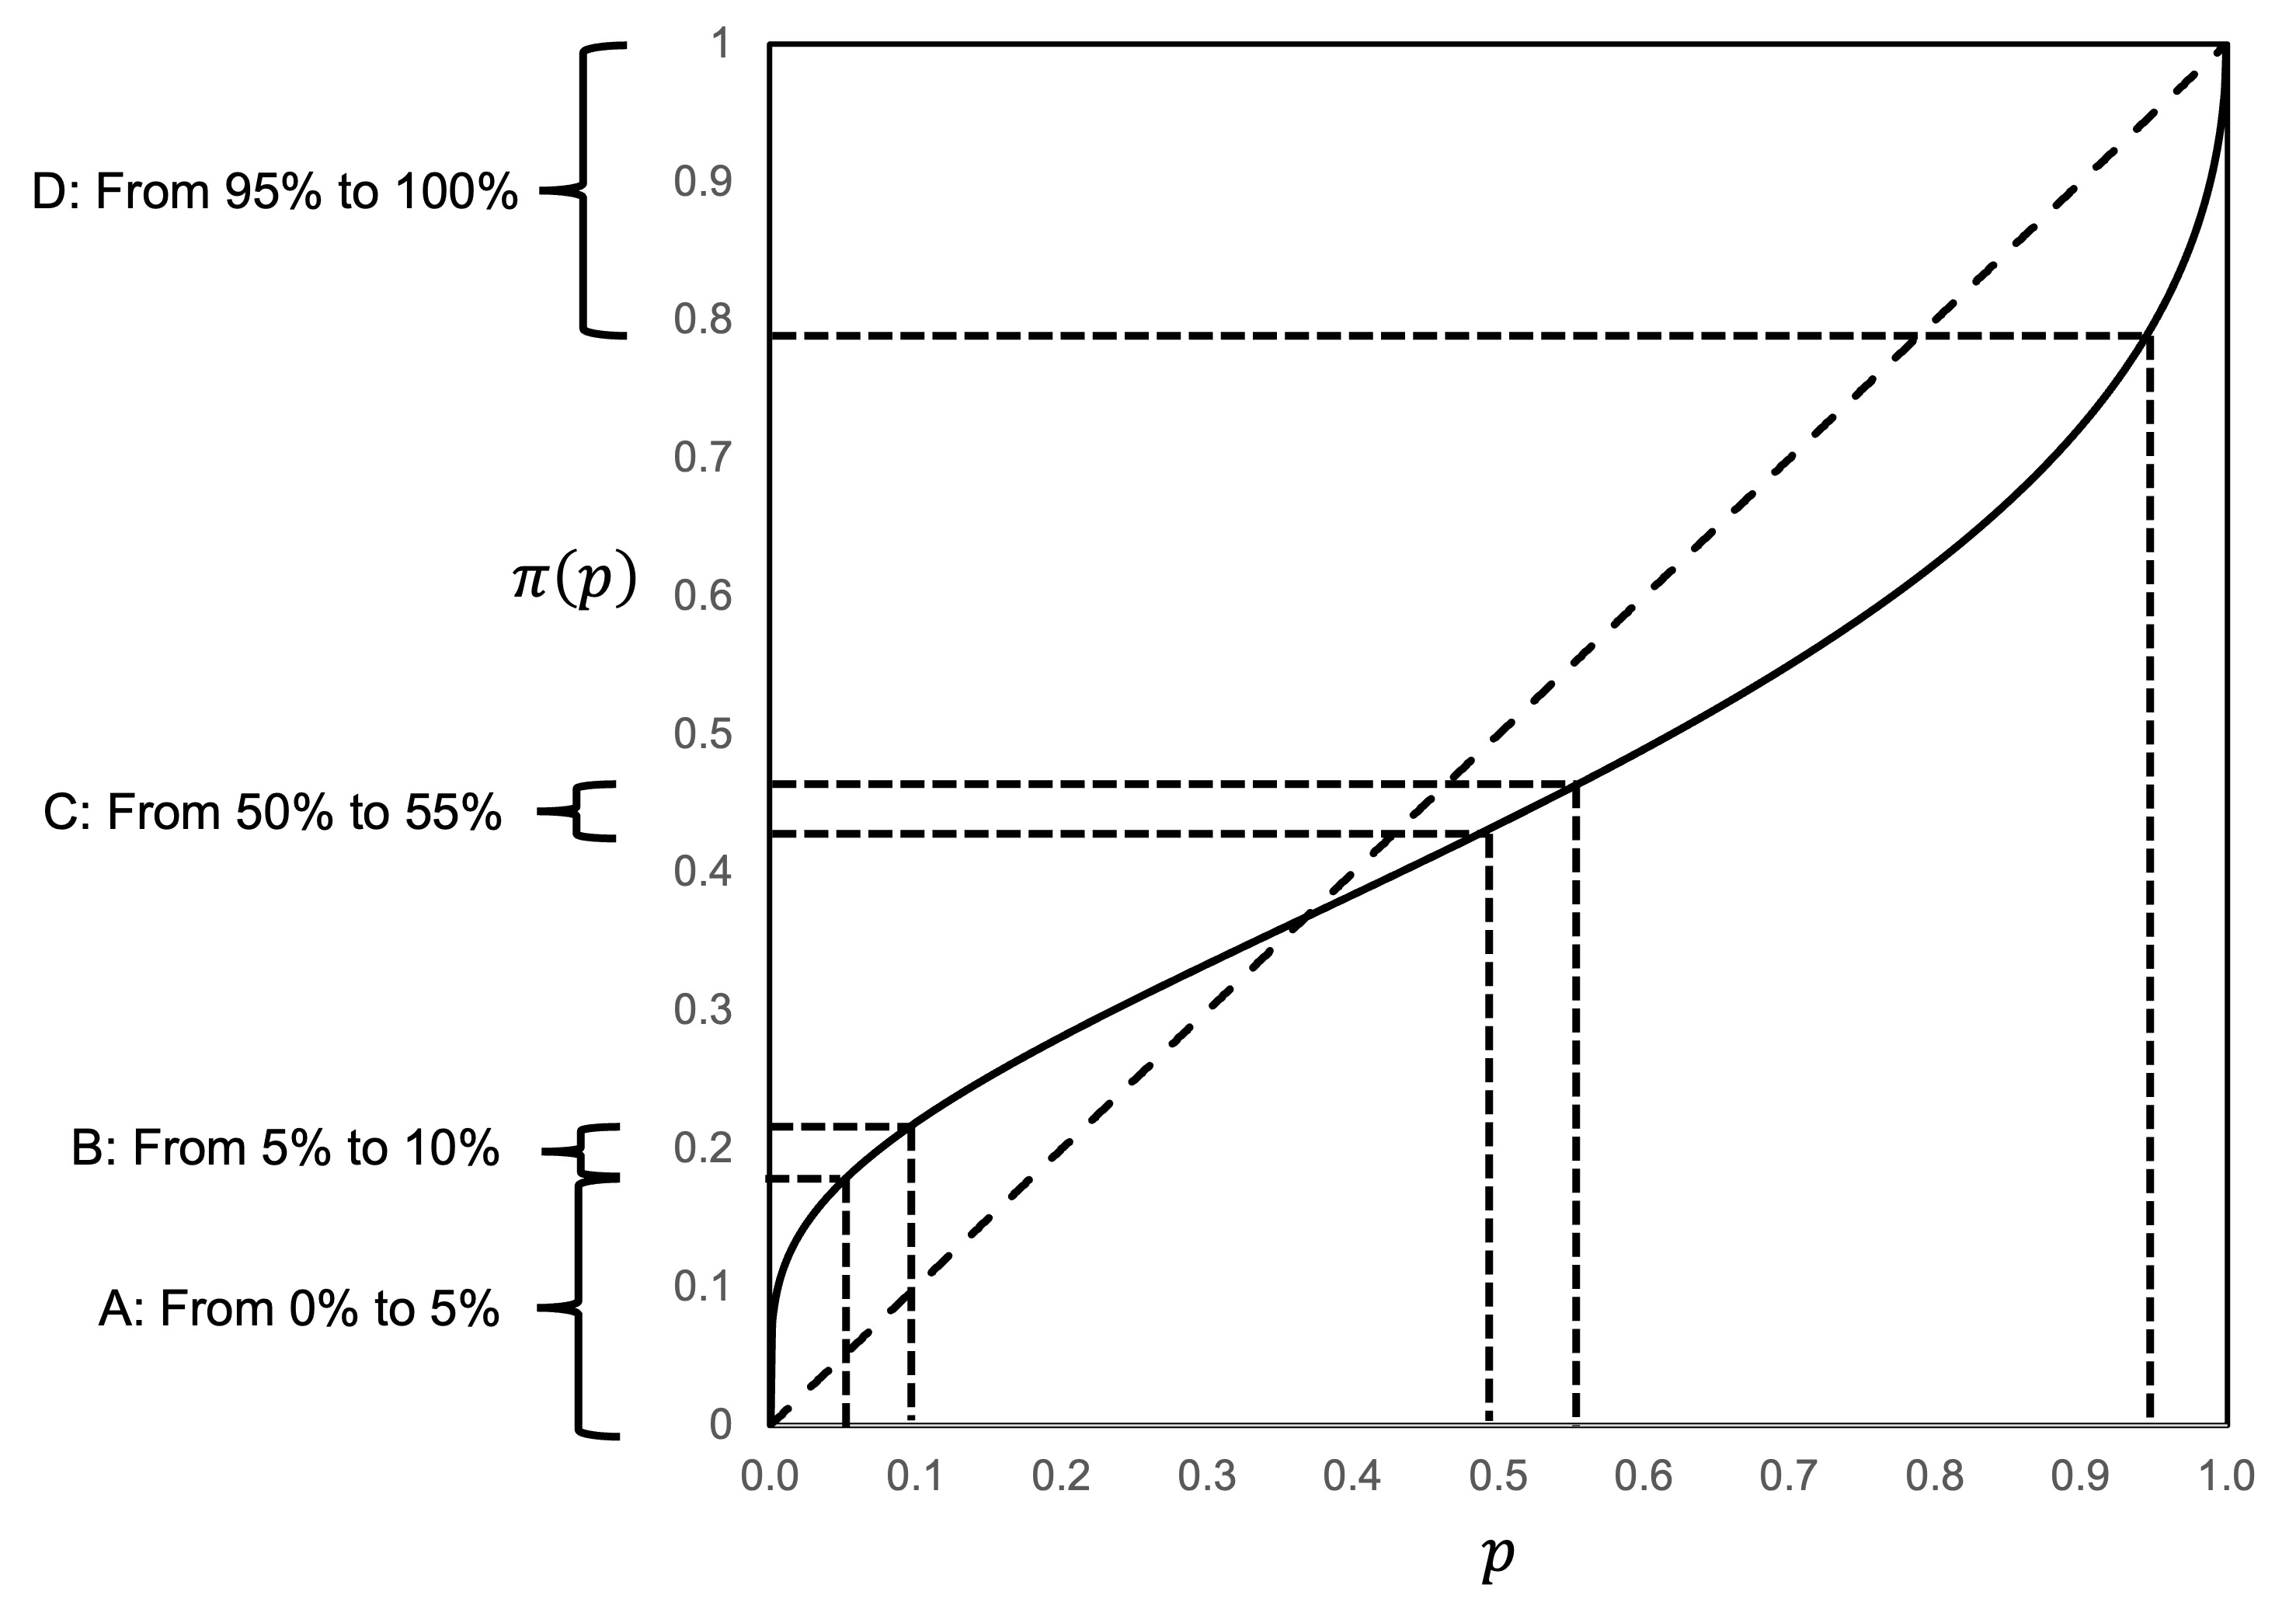
\includegraphics{prospect-theory/img/Exercise_Q1.jpg}

\end{tcolorbox}

\hypertarget{bitcoin}{%
\section{Bitcoin}\label{bitcoin}}

Edna, Ferdinand and Gretel each bought some Bitcoin at \$50,000. The
price rose to \$80,000 and then dropped to \$60,000, at which time they
sold it.

All three are loss averse and have the following reference-dependent
value function:

\[
v(x)=\left\{\begin{matrix}
x \quad &\textrm{where} \quad x \geq 0\\
2x \quad &\textrm{where} \quad x < 0
\end{matrix}\right.
\]

Edna uses the purchase price as her reference point. Ferdinand uses the
peak price as his reference point. Gretel uses the sale price as her
reference point.

What is the change in value for each person? Who is happiest?

\begin{tcolorbox}[enhanced jigsaw, title=\textcolor{quarto-callout-tip-color}{\faLightbulb}\hspace{0.5em}{Answer}, toprule=.15mm, colback=white, breakable, titlerule=0mm, colframe=quarto-callout-tip-color-frame, coltitle=black, opacityback=0, rightrule=.15mm, colbacktitle=quarto-callout-tip-color!10!white, bottomtitle=1mm, opacitybacktitle=0.6, arc=.35mm, bottomrule=.15mm, toptitle=1mm, leftrule=.75mm, left=2mm]

Value for Edna:

\begin{align*}
v(x)&=v(60-50) \\
&=10
\end{align*}

Value for Ferdinand:

\begin{align*}
v(x)&=v(60-80) \\
&=-2\times 30 \\
&=-60
\end{align*}

Value for Gretel:

\begin{align*}
v(x)&=v(60-60) \\
&=0
\end{align*}

Edna is happiest whereas Ferdinand is most disappointed. Both Edna and
Gretel see the peak price as a foregone gain, whereas Ferdinand sees the
failure to sell at the peak as a loss.

\end{tcolorbox}

\hypertarget{reference-points-1}{%
\section{Reference points}\label{reference-points-1}}

Megan has the following reference-dependent value function:

\[
v(x)=\left\{\begin{matrix}
x \quad &\textrm{where} \quad x \geq 0\\
2x \quad &\textrm{where} \quad x < 0
\end{matrix}\right.
\]

where \(x\) is the realised outcome relative to the reference point.

a) If you look at \(v(x)\), we expect Megan to be:

\begin{itemize}
\tightlist
\item
  loss averse
\item
  have no decreased sensitivity to changes of greater magnitude.
\end{itemize}

Why?

\begin{tcolorbox}[enhanced jigsaw, title=\textcolor{quarto-callout-tip-color}{\faLightbulb}\hspace{0.5em}{Answer}, toprule=.15mm, colback=white, breakable, titlerule=0mm, colframe=quarto-callout-tip-color-frame, coltitle=black, opacityback=0, rightrule=.15mm, colbacktitle=quarto-callout-tip-color!10!white, bottomtitle=1mm, opacitybacktitle=0.6, arc=.35mm, bottomrule=.15mm, toptitle=1mm, leftrule=.75mm, left=2mm]

Megan is loss averse as the slope of the value function in the loss
domain is steeper than in the gain domain. One unit of loss leads to a
greater change in value than one unit of gain.

There is no decreases sensitivity as the value function is linear in
both domains. Sensitivity is constant. As the size of the loss or gain
increases, the change in value remains constant despite the increasing
magnitude.

\end{tcolorbox}

b) Assume Megan has received a birthday card from her aunt, which some
years contains \$25 and other years contains nothing.

She opens the card and it contains \$10.

Consider two alternative reference points: Megan is pessimistic and
expects no money in the card, and Megan is optimistic and expects \$25.

Compute Megan's value under each reference point. Which reference point
yields higher value?

\begin{tcolorbox}[enhanced jigsaw, title=\textcolor{quarto-callout-tip-color}{\faLightbulb}\hspace{0.5em}{Answer}, toprule=.15mm, colback=white, breakable, titlerule=0mm, colframe=quarto-callout-tip-color-frame, coltitle=black, opacityback=0, rightrule=.15mm, colbacktitle=quarto-callout-tip-color!10!white, bottomtitle=1mm, opacitybacktitle=0.6, arc=.35mm, bottomrule=.15mm, toptitle=1mm, leftrule=.75mm, left=2mm]

The value of the \$10 from the reference point of expecting nothing is:

\begin{align*}
v(x)&=v(10) \\[6pt]
&=10
\end{align*}

\newpage

The value of the \$10 from the reference point of expecting \$25 is:

\begin{align*}
v(x)&=v(10-25) \\[6pt]
&=2*(-15) \\[6pt]
&=-30
\end{align*}

Megan has higher value when she does not expect to receive any money.
She gets the value of a gain of \$10. If she expected the \$25, she
suffered the value of a loss of \$15.

\end{tcolorbox}

c) Megan has received the \$10 in the card and a piece of birthday cake.
Her value function over money and pieces of birthday cake is:

\[
v(x)=v(m-r_m)+v(4c-4r_c)
\]

Where \(m\) is the amount of money she receives, \(r_m\) is her
reference point of how much money she expects, \(c\) is how many pieces
of birthday cake she receives and \(r_c\) is how many pieces of birthday
cake she expects.

To illustrate how this value function works, imagine Megan expects two
pieces of cake and her dog jumps onto the table and eats one of them.
Her change in the value function is:

\begin{align*}
v(x)&=v(4c-4r_c) \\
&=v(4\times 1-4\times 2) \\
&=v(-4)
\end{align*}

As \(v(x)=2x\) when \(x<0\):

\[
v(-4)=-8
\]

For this question, assume Megan does not believe that she will receive
any money and she expects to eat two pieces of birthday cake. Her
reference point is therefore \(r_m=0\) and \(r_c=2\). She receives \$10
from her aunt.

Her brother - who loves cake - offers to buy one of her pieces of
birthday cake. What price \(p_s\) would make Megan indifferent between
selling and keeping the piece of cake?

\begin{tcolorbox}[enhanced jigsaw, title=\textcolor{quarto-callout-tip-color}{\faLightbulb}\hspace{0.5em}{Answer}, toprule=.15mm, colback=white, breakable, titlerule=0mm, colframe=quarto-callout-tip-color-frame, coltitle=black, opacityback=0, rightrule=.15mm, colbacktitle=quarto-callout-tip-color!10!white, bottomtitle=1mm, opacitybacktitle=0.6, arc=.35mm, bottomrule=.15mm, toptitle=1mm, leftrule=.75mm, left=2mm]

Megan will be indifferent when the value from each option is the same:

\begin{align*}
\underbrace{v(10-0+p_s)}_{\substack{\textrm{Value from} \\ \textrm{unexpected} \\ \textrm{money plus} \\  \textrm{payment} \\ \textrm{for cake}}}+
\underbrace{v(4\times 1-4\times 2)}_{\substack{\textrm{Value lost from} \\ \textrm{giving up cake}}}
&=\underbrace{v(10-0)}_{\substack{\textrm{Value from} \\ \textrm{unexpected} \\ \textrm{money}}}+
v\underbrace{(4\times 2-4\times 2)}_{\substack{\textrm{Value of} \\ \textrm{keeping cake}}} \\[12pt]
v(10+p_s)+v(-4)&=v(10)+v(0) \\[6pt]
10+p_s-8&=10\\[6pt]
p_s&=8
\end{align*}

\end{tcolorbox}

d) Assume that Megan expects to receive only one piece of birthday cake.
Her brother then offers to sell her his piece of cake. For \(r_m=0\) and
\(r_c=1\), what price \(p_b\) would make Megan indifferent between
buying the cake and eating only her own piece?

\begin{tcolorbox}[enhanced jigsaw, title=\textcolor{quarto-callout-tip-color}{\faLightbulb}\hspace{0.5em}{Answer}, toprule=.15mm, colback=white, breakable, titlerule=0mm, colframe=quarto-callout-tip-color-frame, coltitle=black, opacityback=0, rightrule=.15mm, colbacktitle=quarto-callout-tip-color!10!white, bottomtitle=1mm, opacitybacktitle=0.6, arc=.35mm, bottomrule=.15mm, toptitle=1mm, leftrule=.75mm, left=2mm]

Megan will be indifferent when the value from each option is the same:

\begin{align*}
\underbrace{v(10-0-p_b)}_{\substack{\textrm{Value from} \\ \textrm{unexpected} \\ \textrm{money minus} \\  \textrm{payment} \\ \textrm{for cake}}}+
\underbrace{v(4\times 2-4\times 1)}_{\substack{\textrm{Value gained from} \\ \textrm{buying cake}}}
&=\underbrace{v(10-0)}_{\substack{\textrm{Value from} \\ \textrm{unexpected} \\ \textrm{money}}}+
v\underbrace{(4\times 1-4\times 1)}_{\substack{\textrm{Value of} \\ \textrm{only one piece}}} \\[12pt]
v(10-p_b)+v(4)&=v(10)+v(0) \\[6pt]
10-p_b+4&=10\\[6pt]
p_b&=4
\end{align*}

\end{tcolorbox}

e) Why is there a difference between the price at which Megan was
willing to sell cake in part c) compared to the price she was willing to
pay in part d)?

\begin{tcolorbox}[enhanced jigsaw, title=\textcolor{quarto-callout-tip-color}{\faLightbulb}\hspace{0.5em}{Answer}, toprule=.15mm, colback=white, breakable, titlerule=0mm, colframe=quarto-callout-tip-color-frame, coltitle=black, opacityback=0, rightrule=.15mm, colbacktitle=quarto-callout-tip-color!10!white, bottomtitle=1mm, opacitybacktitle=0.6, arc=.35mm, bottomrule=.15mm, toptitle=1mm, leftrule=.75mm, left=2mm]

The willingness to accept in part c) is higher than the willingness to
pay in part d) as in part c) the foregone cake is coded as a loss. This
loss reduces value at twice the rate of a gain in cake. The payment for
the cake in both parts is in the gain domain due to the birthday present
of \$10, so the payment received or paid is given less weight than any
loss.

\end{tcolorbox}

\hypertarget{saving-on-a-purchase}{%
\section{Saving on a purchase}\label{saving-on-a-purchase}}

Consider the following two scenarios:

A) You are considering buying a new type of coffee bean for your home
coffee machine. It costs \$50 at your local hipster cafe, but you
discover that it is for sale for \$40 at the supermarket 20 minutes
drive from your home. Do you make the trip?

B) You are considering buying a new laptop. It costs \$1990 at your
local computer store, but you discover that it is for sale for \$1980 at
another computer store 20 minutes drive from your home. Do you make the
trip?

When people are presented with scenarios such as this, they tend to
report that they are less likely to make the trip in Scenario B for the
more expensive product.

Explain how an S-shaped value function with diminishing value in both
gains and losses could result in this behaviour.

\begin{tcolorbox}[enhanced jigsaw, title=\textcolor{quarto-callout-tip-color}{\faLightbulb}\hspace{0.5em}{Answer}, toprule=.15mm, colback=white, breakable, titlerule=0mm, colframe=quarto-callout-tip-color-frame, coltitle=black, opacityback=0, rightrule=.15mm, colbacktitle=quarto-callout-tip-color!10!white, bottomtitle=1mm, opacitybacktitle=0.6, arc=.35mm, bottomrule=.15mm, toptitle=1mm, leftrule=.75mm, left=2mm]

Diminishing value means that the absolute difference between \(v(-40)\)
and \(v(-50)\) is much larger than the absolute difference between
\(v(-1980)\) and \(v(-1990)\). For example, suppose the value function
was:

\[
v(x)=\left\{\begin{matrix}
x^\frac{1}{2} \quad &\textrm{where} \quad x \geq 0\\
-2(-x)^\frac{1}{2} \quad &\textrm{where} \quad x < 0
\end{matrix}\right.
\]

\newpage

This would mean that the difference between \(v(-40)\) and \(v(-50)\)
is:

\begin{align*}
v(-40)-v(-50)&=-2(40^\frac{1}{2}-50^\frac{1}{2}) \\
&=1.493025
\end{align*}

The difference between \(v(-1980)\) and \(v(-1990)\) is:

\begin{align*}
v(-1980)-v(-1990)&=-2(1980^\frac{1}{2}-1990^\frac{1}{2}) \\
&=0.2244502
\end{align*}

Much less value is gained by driving for the 20 minutes across town for
the computer.

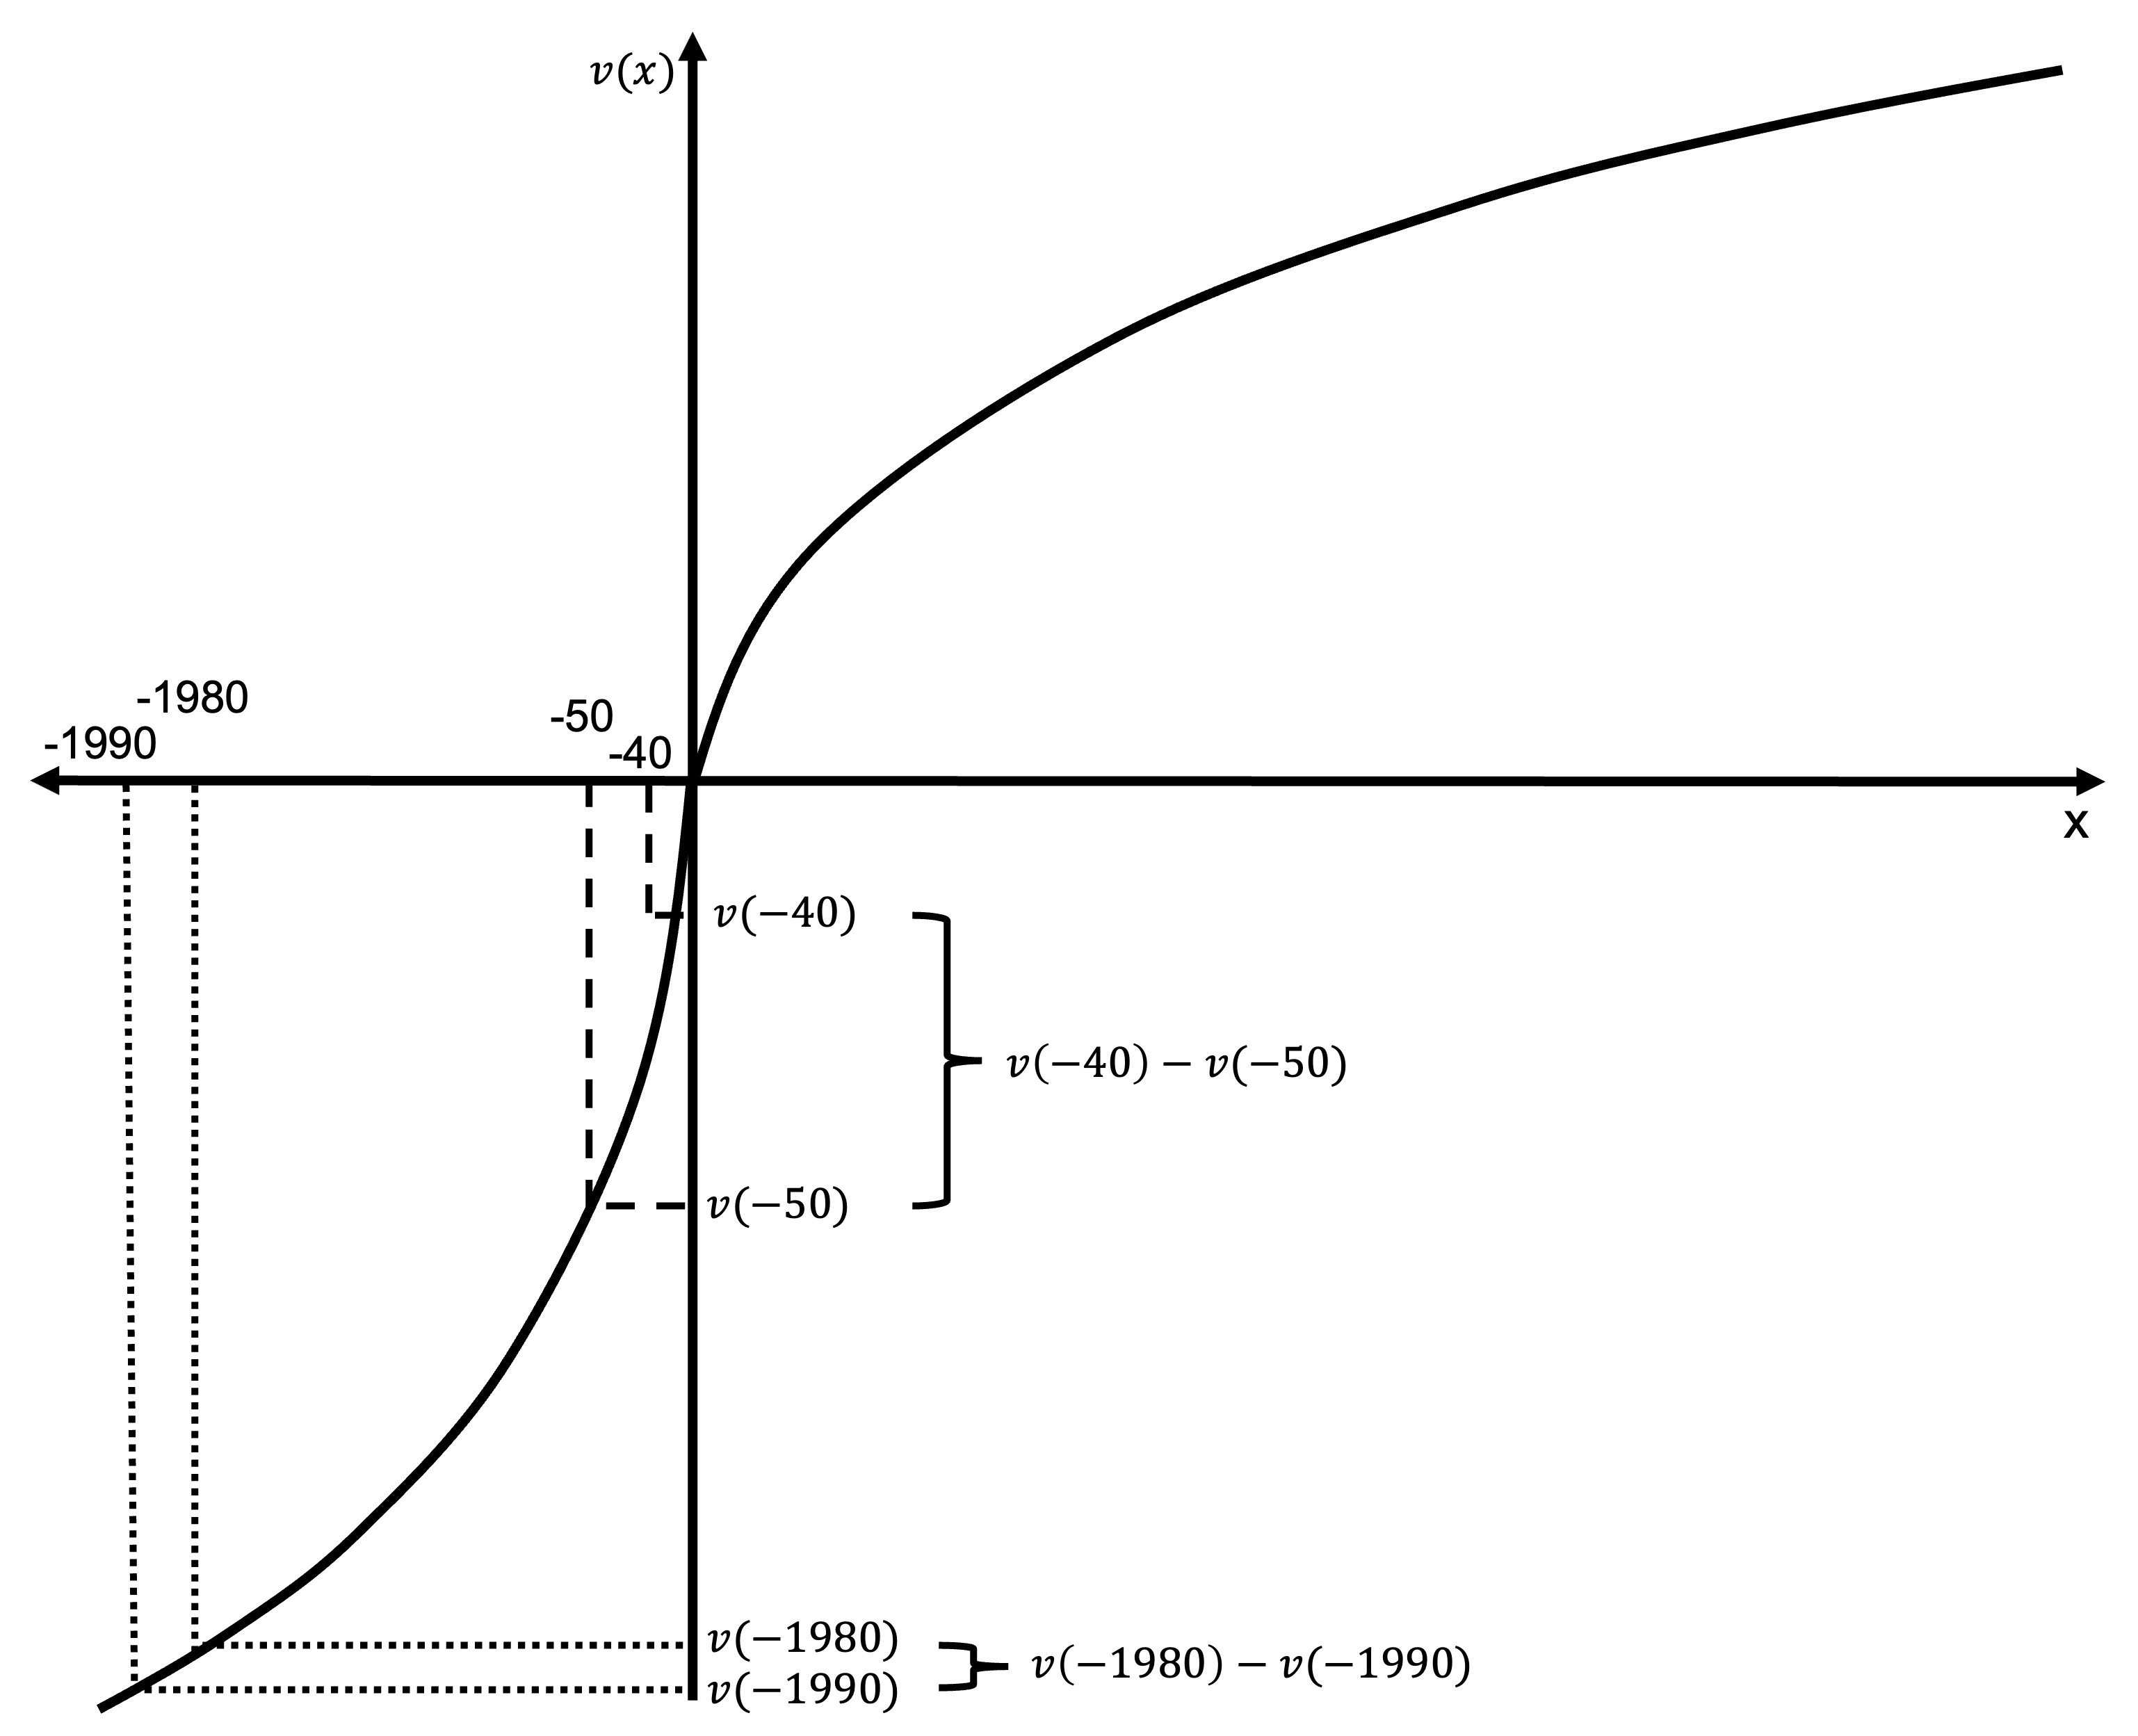
\includegraphics[width=0.7\textwidth,height=\textheight]{prospect-theory/img/Exercise_Q4.jpg}

\end{tcolorbox}

\hypertarget{a-6040-gamble-2}{%
\section{A 60:40 gamble}\label{a-6040-gamble-2}}

Suppose an agent has the following reference-dependent value function:

\[
v(x)=\left\{\begin{matrix}
x^{3/4} \qquad &\textrm{where} \space &x \geq 0\\
-2(-x)^{3/4} \quad &\textrm{where} \space &x < 0
\end{matrix}\right.
\]

Where \(x\) is the realised outcome relative to the reference point.

Assume that the agent's reference point is the status quo and the agent
is offered the gamble A:

\[(\$100, 0.6; −\$100, 0.4)\]

a) Will they want to play this gamble? Why?

\begin{tcolorbox}[enhanced jigsaw, title=\textcolor{quarto-callout-tip-color}{\faLightbulb}\hspace{0.5em}{Answer}, toprule=.15mm, colback=white, breakable, titlerule=0mm, colframe=quarto-callout-tip-color-frame, coltitle=black, opacityback=0, rightrule=.15mm, colbacktitle=quarto-callout-tip-color!10!white, bottomtitle=1mm, opacitybacktitle=0.6, arc=.35mm, bottomrule=.15mm, toptitle=1mm, leftrule=.75mm, left=2mm]

The utility from the gamble is:

\begin{align*}
V(A)&=0.6v(100)-0.4v(-100) \\
&=0.6\times (100)^{0.75}-0.4\times 2\times (100)^{0.75} \\
&=-6.3245553
\end{align*}

They will not want to play this gamble as it has a negative value for
the agent. They could receive value of 0 by simply not playing.

The reason for this negative value is that the agent is loss averse. The
loss of \$100 is given twice the weight of an equivalent gain, meaning
that they reject the bet despite a win of \$100 being more probable.

\end{tcolorbox}

b) Suppose the agent takes this gamble and loses \$100. They feel bad
about it and perceive it as a loss. Their reference point is unchanged
at the original status quo. They are offered gamble A again? Do they
accept this second time? Why?

\begin{tcolorbox}[enhanced jigsaw, title=\textcolor{quarto-callout-tip-color}{\faLightbulb}\hspace{0.5em}{Answer}, toprule=.15mm, colback=white, breakable, titlerule=0mm, colframe=quarto-callout-tip-color-frame, coltitle=black, opacityback=0, rightrule=.15mm, colbacktitle=quarto-callout-tip-color!10!white, bottomtitle=1mm, opacitybacktitle=0.6, arc=.35mm, bottomrule=.15mm, toptitle=1mm, leftrule=.75mm, left=2mm]

After losing \$100 but not changing their reference point, they have two
possible outcomes relative to their reference point: recovery of their
loss of \$100 so they come out even and a loss of \$200 (losing \$100
twice).

\begin{align*}
V(A)&=0.6v(-100+10)-0.4v(-100-100) \\
&=0.6\times (0)^{0.75}-0.4\times 2\times (200)^{0.75} \\
&=-42.5463672
\end{align*}

The utility of not playing the gamble involves remaining with a loss of
\$100:

\begin{align*}
V(\neg A)&=v(-100) \\
&=-2\times (100)^{0.75} \\
&=-63.2455532
\end{align*}

They will now want to play the gamble as it has a greater value than
staying with their current loss. The reason the gamble becomes
attractive is because it gives an opportunity to recover the loss. The
agent is risk seeking over the loss domain.

\end{tcolorbox}

c) The agent is offered a new job for which they receive a \$50,000
sign-on bonus. They adapt to their new wealth, so their reference point
changes to accommodate their new situation. They are now offered gamble
A again. Do they accept? Why?

\begin{tcolorbox}[enhanced jigsaw, title=\textcolor{quarto-callout-tip-color}{\faLightbulb}\hspace{0.5em}{Answer}, toprule=.15mm, colback=white, breakable, titlerule=0mm, colframe=quarto-callout-tip-color-frame, coltitle=black, opacityback=0, rightrule=.15mm, colbacktitle=quarto-callout-tip-color!10!white, bottomtitle=1mm, opacitybacktitle=0.6, arc=.35mm, bottomrule=.15mm, toptitle=1mm, leftrule=.75mm, left=2mm]

With their new reference point, this question is effectively the same as
part a). They will refuse the bet.

\end{tcolorbox}

\hypertarget{a-5050-gamble-2}{%
\section{A 50:50 gamble}\label{a-5050-gamble-2}}

Suppose Tim has the following reference-dependent value function:

\[
v(x)=\left\{\begin{matrix}
x^{1/2} \qquad &\textrm{where} &\space x \geq 0\\
-2(-x)^{1/2} \quad &\textrm{where} &\space x < 0 
\end{matrix}\right.
\]

\(x\) is the change in Tim's position relative to his reference point.

a) What feature of Tim's value function leads to loss aversion? Explain.

\begin{tcolorbox}[enhanced jigsaw, title=\textcolor{quarto-callout-tip-color}{\faLightbulb}\hspace{0.5em}{Answer}, toprule=.15mm, colback=white, breakable, titlerule=0mm, colframe=quarto-callout-tip-color-frame, coltitle=black, opacityback=0, rightrule=.15mm, colbacktitle=quarto-callout-tip-color!10!white, bottomtitle=1mm, opacitybacktitle=0.6, arc=.35mm, bottomrule=.15mm, toptitle=1mm, leftrule=.75mm, left=2mm]

The part of the value function that applies when \(x<0\) is increased by
a factor of two relative to that part of the value function for when
\(x>0\). This is done by multiplying the bottom portion by 2.

\end{tcolorbox}

b) Tim considers the gamble A: (\$250, 0.5; -\$100, 0.5).

\begin{enumerate}
\def\labelenumi{\roman{enumi})}
\tightlist
\item
  Will Tim want to play this gamble?
\end{enumerate}

\begin{tcolorbox}[enhanced jigsaw, title=\textcolor{quarto-callout-tip-color}{\faLightbulb}\hspace{0.5em}{Answer}, toprule=.15mm, colback=white, breakable, titlerule=0mm, colframe=quarto-callout-tip-color-frame, coltitle=black, opacityback=0, rightrule=.15mm, colbacktitle=quarto-callout-tip-color!10!white, bottomtitle=1mm, opacitybacktitle=0.6, arc=.35mm, bottomrule=.15mm, toptitle=1mm, leftrule=.75mm, left=2mm]

\begin{align*}
V(A)&=p_1v(x_1)+p_2v(x_2) \\
&=0.5v(\$250)+0.5v(-\$100) \\
&=0.5*250^{1/2}-0.5*2*100^{1/2} \\
&=-2.0943058
\end{align*}

Tim has negative value from the gamble, when he could simply have zero
value by declining. He rejects.

\end{tcolorbox}

\begin{enumerate}
\def\labelenumi{\roman{enumi})}
\setcounter{enumi}{1}
\tightlist
\item
  Explain what features of the value function lead him to accept or
  reject the gamble.
\end{enumerate}

\begin{tcolorbox}[enhanced jigsaw, title=\textcolor{quarto-callout-tip-color}{\faLightbulb}\hspace{0.5em}{Answer}, toprule=.15mm, colback=white, breakable, titlerule=0mm, colframe=quarto-callout-tip-color-frame, coltitle=black, opacityback=0, rightrule=.15mm, colbacktitle=quarto-callout-tip-color!10!white, bottomtitle=1mm, opacitybacktitle=0.6, arc=.35mm, bottomrule=.15mm, toptitle=1mm, leftrule=.75mm, left=2mm]

Two features of the value function lead him to reject:

\begin{itemize}
\tightlist
\item
  Tim is loss averse (the -2 in the bottom equation), which leads him to
  give twice the weight to losses relative to an equal sized gain.
\item
  Tim has diminishing sensitivity to losses and gains. The larger gain
  is reduced proportionately more by this diminishing sensitivity.
\end{itemize}

\end{tcolorbox}

c) Suppose Tim were to experience a large positive or negative shock to
his wealth that does not immediately change his reference point. Could
either shock cause him to change his decision concerning gamble A?
Explain.

\begin{tcolorbox}[enhanced jigsaw, title=\textcolor{quarto-callout-tip-color}{\faLightbulb}\hspace{0.5em}{Answer}, toprule=.15mm, colback=white, breakable, titlerule=0mm, colframe=quarto-callout-tip-color-frame, coltitle=black, opacityback=0, rightrule=.15mm, colbacktitle=quarto-callout-tip-color!10!white, bottomtitle=1mm, opacitybacktitle=0.6, arc=.35mm, bottomrule=.15mm, toptitle=1mm, leftrule=.75mm, left=2mm]

Both a positive and negative shock could lead Tim to change his
decision.

A large positive shock would place the entire bet into the gain domain.
That would remove loss aversion as a factor in rejecting the bet. Given
the high expected value, that would likely be sufficient for him to
accept. However, a large shock would also place Tim further up the value
function to a region where it is more linear (i.e.~he is less risk
averse). This will also increase the tendency to accept the bet.

A large negative shock would place the entire bet into the loss domain.
That would remove loss aversion as a factor in rejecting the bet as
there is no gain against which the loss can be given relatively greater
weight. Due to diminishing sensitivity to losses, Tim is also risk
seeking in the loss domain. This would lead him to accept any bet with a
positive expected value.

\end{tcolorbox}

\hypertarget{insurance-1}{%
\section{Insurance}\label{insurance-1}}

Explain how probability weighting as proposed under Prospect Theory can
lead a person to simultaneously gamble and purchase insurance.

\begin{tcolorbox}[enhanced jigsaw, title=\textcolor{quarto-callout-tip-color}{\faLightbulb}\hspace{0.5em}{Answer}, toprule=.15mm, colback=white, breakable, titlerule=0mm, colframe=quarto-callout-tip-color-frame, coltitle=black, opacityback=0, rightrule=.15mm, colbacktitle=quarto-callout-tip-color!10!white, bottomtitle=1mm, opacitybacktitle=0.6, arc=.35mm, bottomrule=.15mm, toptitle=1mm, leftrule=.75mm, left=2mm]

Decisions under Prospect Theory are the outcome of two factors:

\begin{itemize}
\tightlist
\item
  The value function that gives a value to each outcome relative to a
  reference point
\item
  The probability weighting function that gives a decision weight to the
  probability of each outcome.
\end{itemize}

The Prospect Theory value function leads people to be risk averse in the
domain of gains and risk seeking in the loss domain. This combination
would tend to lead people to purchase neither insurance or lotteries.
Their risk seeking behaviour could lead them to avoid the certain loss
of the insurance premium. They would rather risk the loss of the
insurable asset.

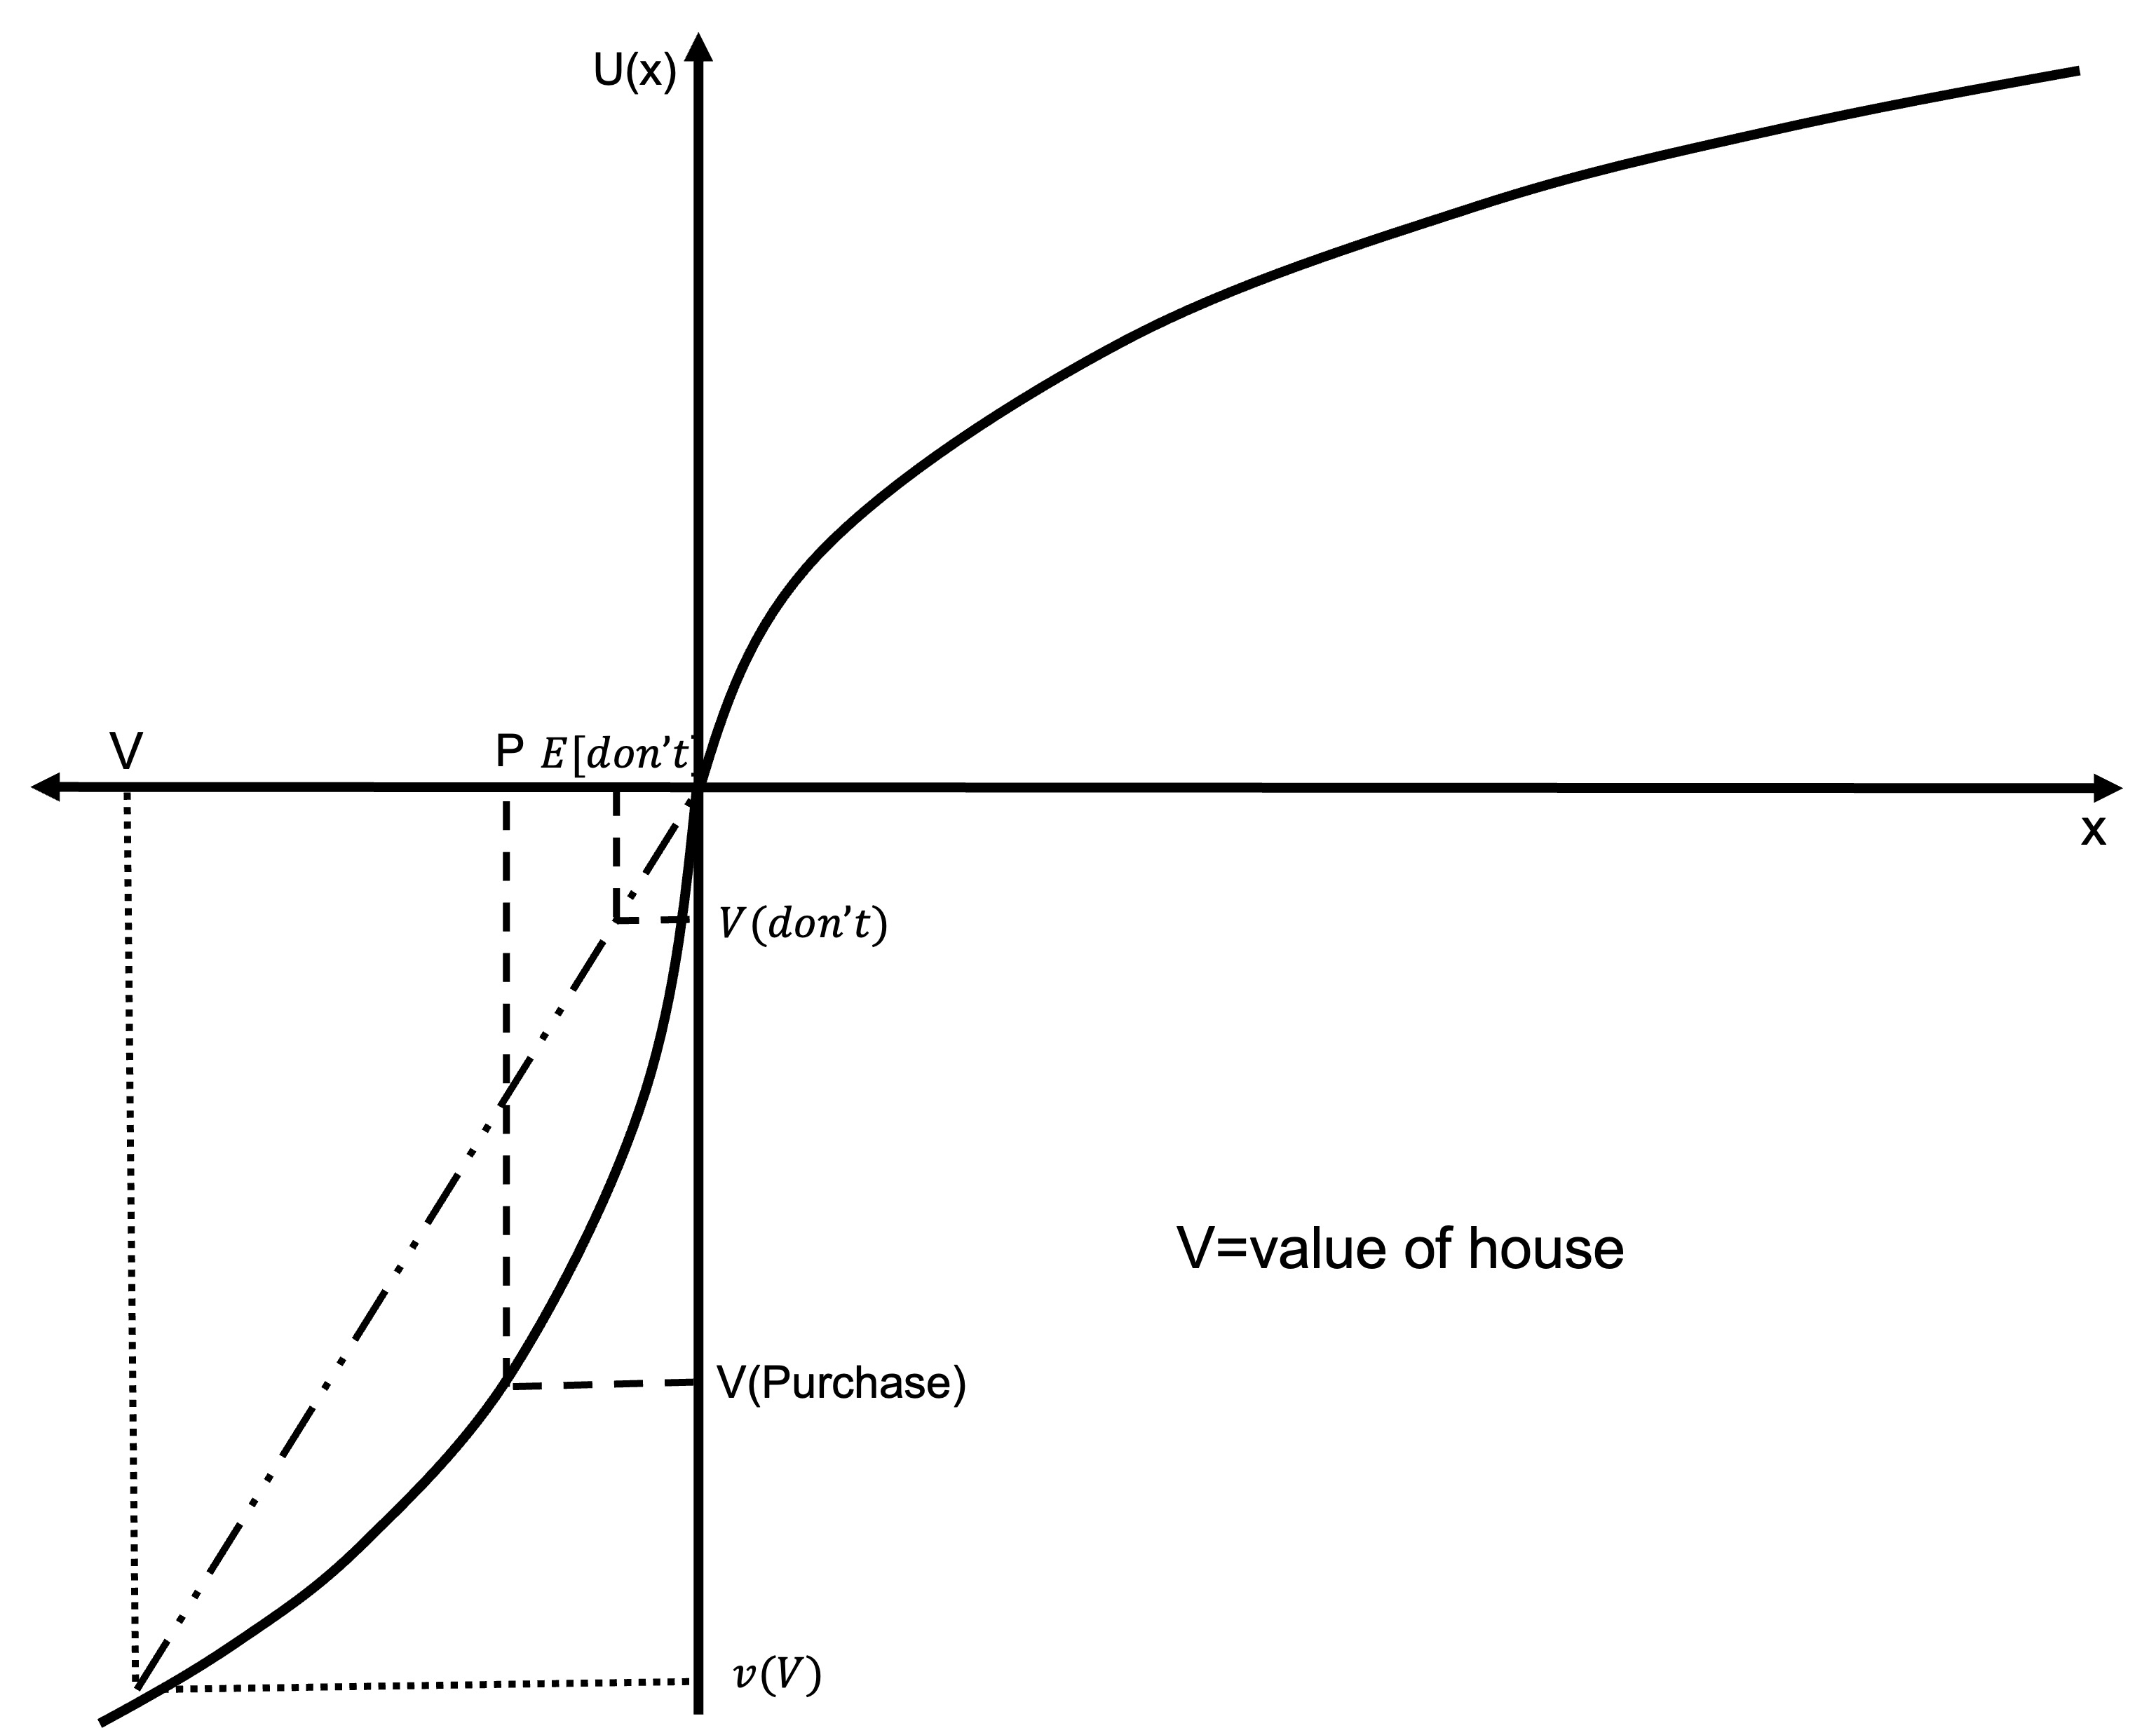
\includegraphics[width=0.48\textwidth,height=\textheight]{prospect-theory/img/Exercise_Q6a.jpg}

Their risk averse behaviour in the domain of gains would make a lottery
with a negative expected value unattractive.

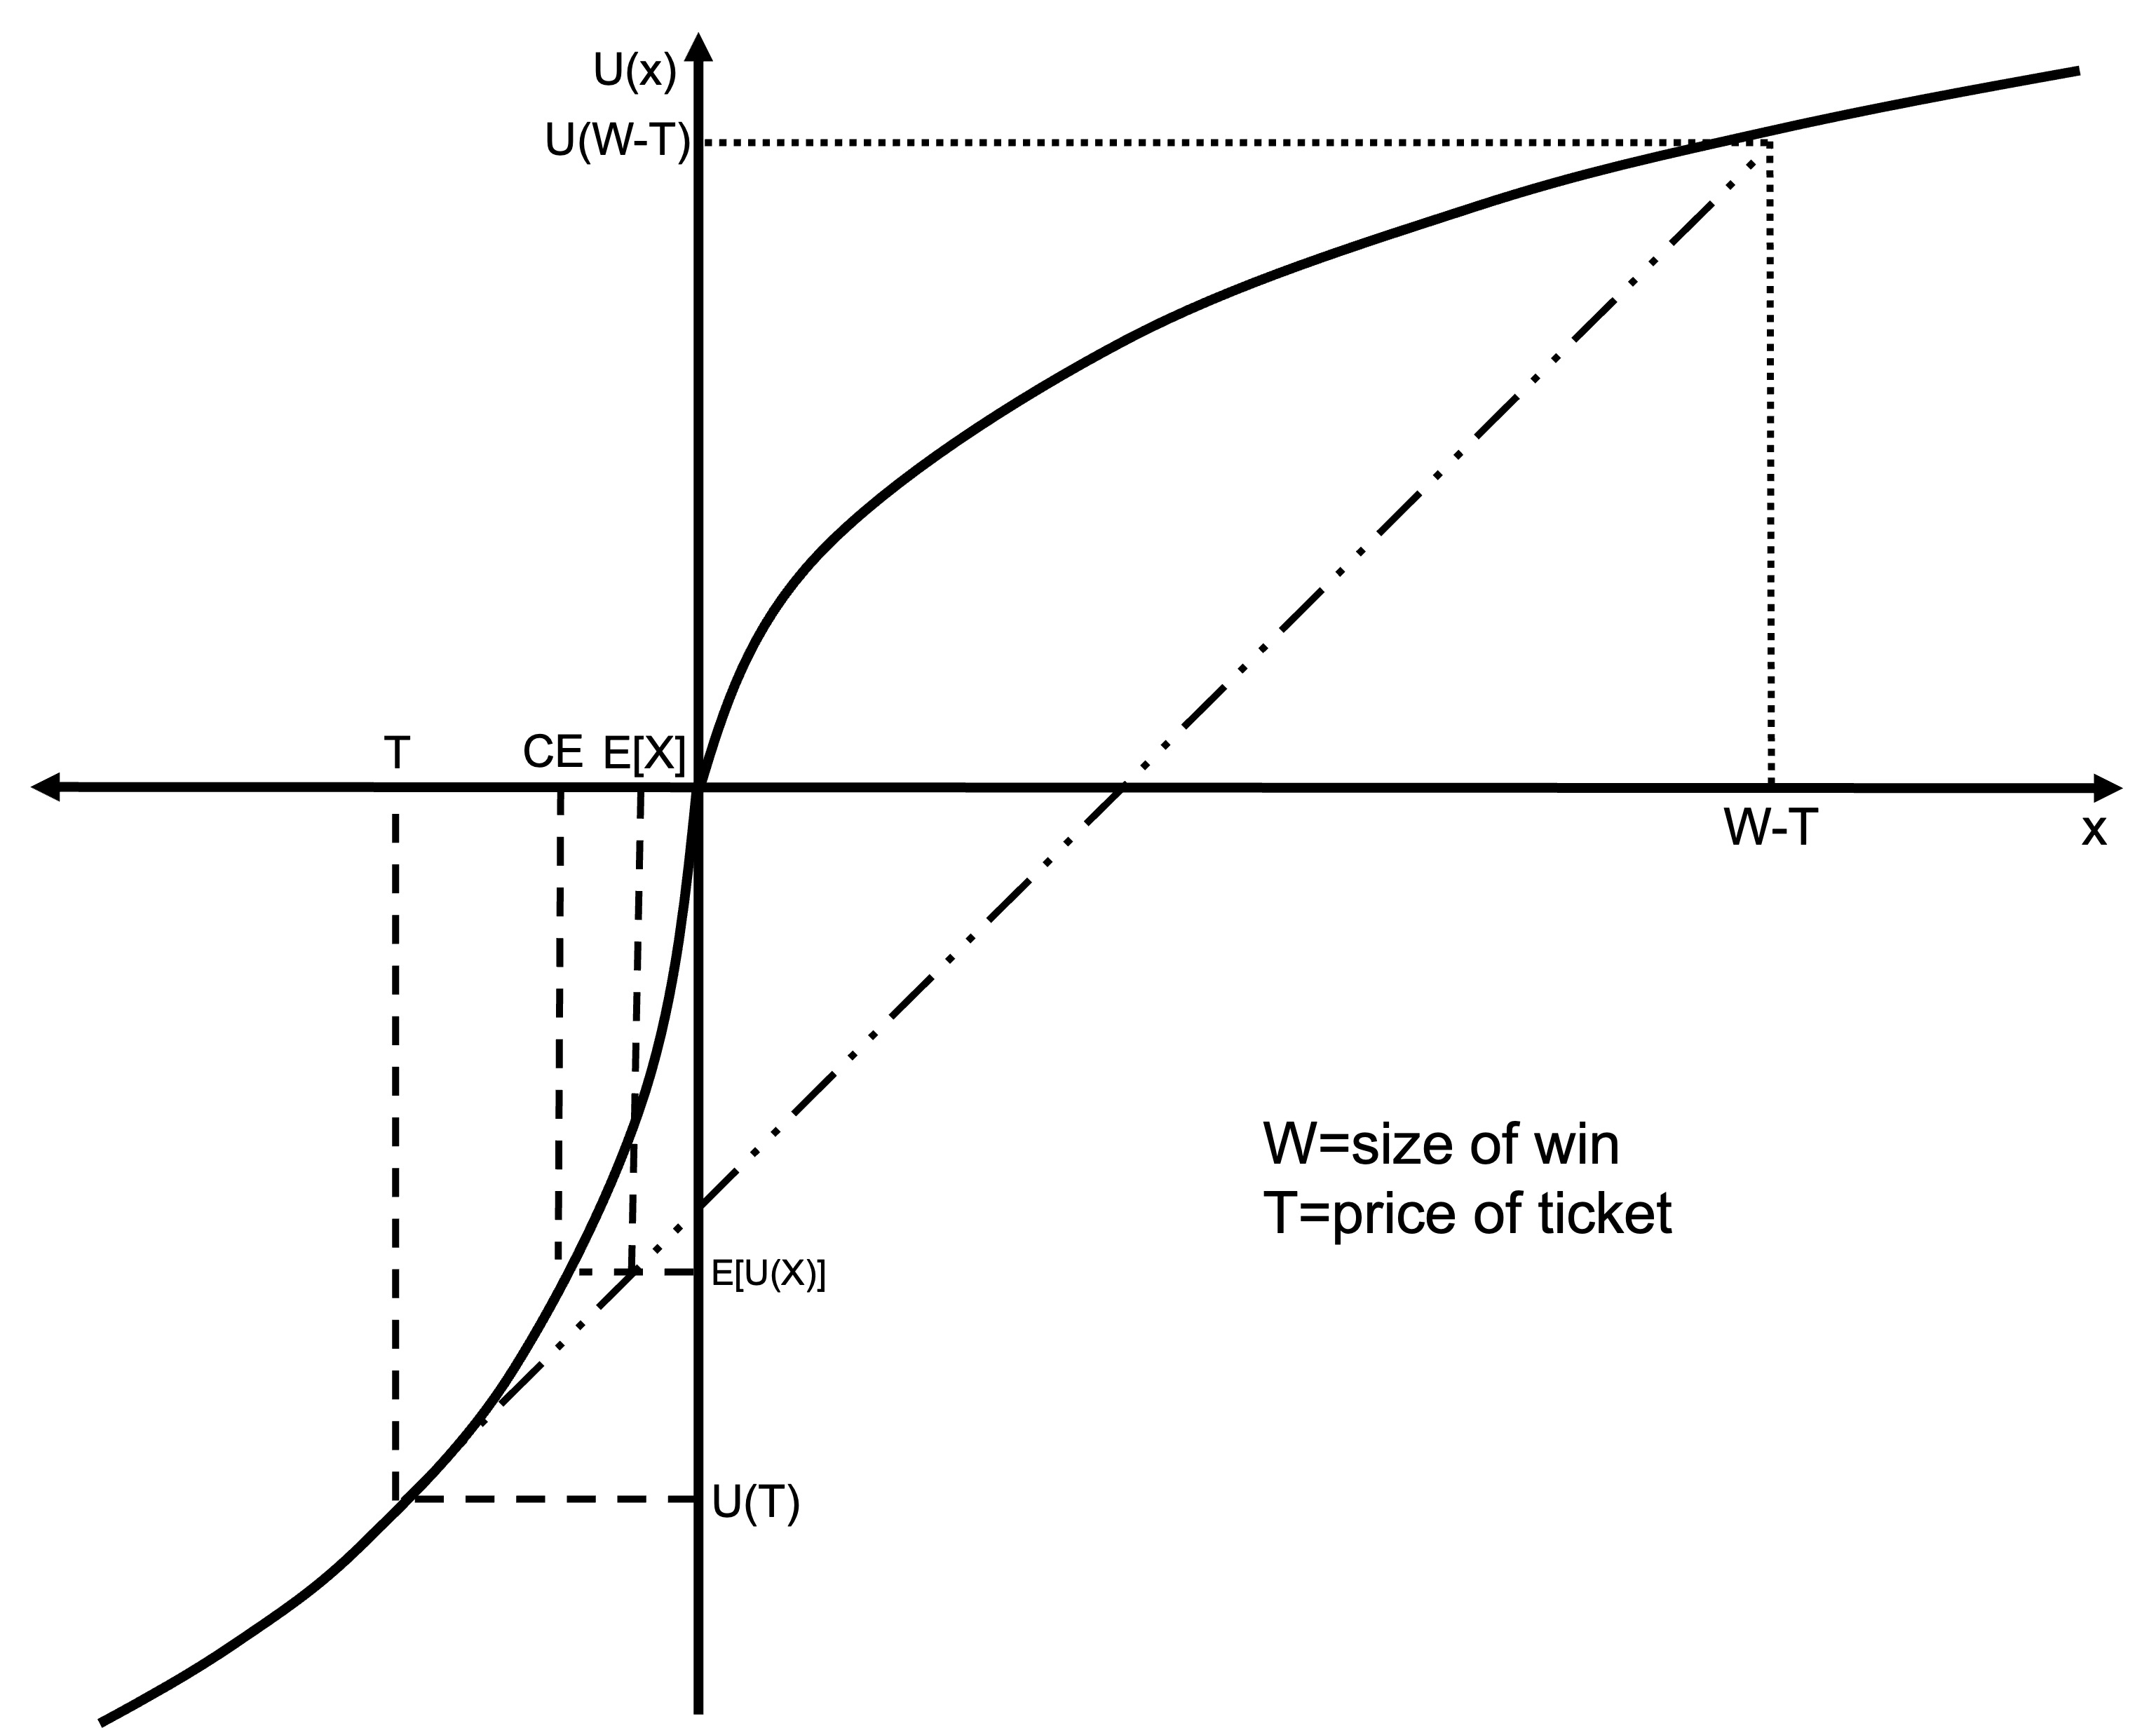
\includegraphics[width=0.48\textwidth,height=\textheight]{prospect-theory/img/Exercise_Q6b.jpg}

However, the probability weighting function can counteract that effect.
By overweighting the small probability of an insurable event or a
lottery win, the agent may decide to insure or purchase a lottery
despite the risk attitudes inherent in the value function.

As an example, consider an agent who overweights a probability of 1 in a
million lottery win by 1,000 times, acting as though they would win the
\$1 million prize once every 1000 lotteries. They also overweight the
probability of a one in a thousand fire that would destroy their million
dollar house by 100 times, acting as though it is a 1-in-10 chance.
(These numbers are extreme, but I am creating a toy example.)

Suppose the lottery ticket is \$1 and their utility function is:

\[
v(x)=\left\{\begin{matrix}
x^{1/2} \quad &\textrm{where} \space &x \geq 0\\
-(-x)^{1/2} \quad &\textrm{where} \space &x < 0
\end{matrix}\right.
\]

Value of purchasing the lottery:

\begin{align*}
v(x)&=\sum_{i=1}^{n} \pi(x_i)v(x_i) \\[6pt]
&=0.001\times (1000000-1)^{1/2}-0.999\times (1)^{1/2} \\[6pt]
&=0.000999
\end{align*}

The value of not purchasing the lottery is zero.

They will purchase the lottery as it has the higher value.

Value of not purchasing insurance, which involves the potential loss of
the house:

\begin{align*}
v(x)&=\sum_{i=1}^{n} \pi(x_i)v(x_i) \\[6pt]
&=-0.1\times (1000000)^{1/2}+0.9\times (0)^{1/2} \\[6pt]
&=-100
\end{align*}

Value of purchasing insurance, which is the certain loss of the premium:

\begin{align*}
v(x)&=\sum_{i=1}^{n} \pi(x_i)v(x_i) \\[6pt]
&=-(1000)^{1/2} \\[6pt]
&=-31.6
\end{align*}

They purchase insurance as it has higher value than not purchasing it.

\end{tcolorbox}

\hypertarget{locking-in-a-win}{%
\section{Locking in a win}\label{locking-in-a-win}}

Amber sued a tabloid newspaper for defamation. The trial has completed
and the judge has retired to make her decision.

Amber's lawyer tells her that she has a 95\% chance of winning and
receiving \$1,000,000 in damages, meaning she has a 5\% chance of
leaving with nothing. (Ignore any potential costs.) She then receives an
offer of settlement from the newspaper for \$800,000. Amber accepts.

Use the fourfold pattern of attitudes to risk under Prospect Theory to
explore why Amber accepted the settlement offer.

\begin{tcolorbox}[enhanced jigsaw, title=\textcolor{quarto-callout-tip-color}{\faLightbulb}\hspace{0.5em}{Answer}, toprule=.15mm, colback=white, breakable, titlerule=0mm, colframe=quarto-callout-tip-color-frame, coltitle=black, opacityback=0, rightrule=.15mm, colbacktitle=quarto-callout-tip-color!10!white, bottomtitle=1mm, opacitybacktitle=0.6, arc=.35mm, bottomrule=.15mm, toptitle=1mm, leftrule=.75mm, left=2mm]

Rejecting the offer has a higher expected value than the value of the
settlement:

\begin{align*}
E[\text{reject}]&=p_{win} x_{win} \\
&=0.95\times 1000000 \\
&=950000
\end{align*}

There are two forces under prospect theory that would lead Amber to take
the option with the lower expected value:

\begin{itemize}
\tightlist
\item
  People are risk averse in the gain domain. Amber would prefer
  certainty to a gamble with the same expected value, and depending on
  the level of risk aversion, would be willing to accept an amount for
  certain lower than the expected value of the bet. That is, the
  certainty equivalent of the gamble would be less than its expected
  value.
\item
  People overweight small probabilities. The 5\% probability of losing
  is likely overweighted by Amber.
\end{itemize}

\end{tcolorbox}

\hypertarget{lotteries}{%
\section{Lotteries}\label{lotteries}}

A common intervention to encourage behaviour change is to offer a
lottery ticket as an incentive. For example, a lottery ticket might be
offered to people who complete a survey.

The government is considering whether it should incentivise vaccination
with either:

\begin{enumerate}
\def\labelenumi{\roman{enumi})}
\item
  a payment of \$10 or
\item
  a lottery ticket with a 1 in a million chance of winning \$10 million.
\end{enumerate}

Use concepts from Prospect Theory to explain why either option might be
more successful.

\begin{tcolorbox}[enhanced jigsaw, title=\textcolor{quarto-callout-tip-color}{\faLightbulb}\hspace{0.5em}{Answer}, toprule=.15mm, colback=white, breakable, titlerule=0mm, colframe=quarto-callout-tip-color-frame, coltitle=black, opacityback=0, rightrule=.15mm, colbacktitle=quarto-callout-tip-color!10!white, bottomtitle=1mm, opacitybacktitle=0.6, arc=.35mm, bottomrule=.15mm, toptitle=1mm, leftrule=.75mm, left=2mm]

There are two opposing forces that could lead to either option being
preferred.

Both the lottery and payment of \$10 are in the gain domain. Under
prospect theory, people tend to be risk averse in the gain domain. This
will make the payment, which has the same expected value as the lottery,
more attractive.

Conversely, under prospect theory people do not weight outcomes directly
by their probability. They apply decision weights that tend to
overweight small probabilities and underweight probabilities just short
of certainty. This means that the small chance of \$10 million will
likely be overweighted. This could lead to the value of the lottery
exceeding that of the certain payment.

Which effect dominates depends on how risk averse people are and how
much they overweight the probability.

\end{tcolorbox}

\part{Intertemporal choice}

Intertemporal choice refers to decisions involving costs and benefits
occurring at different times.

Almost every decision is an intertemporal choice. Intertemporal choices
can be important because:

\begin{itemize}
\tightlist
\item
  feedback may not be immediate (when will you realise your retirement
  savings are inadequate?)
\item
  they may be irreversible (what can you do if you reach retirement age
  with little savings?)
\item
  stakes can be large (health, wealth, career).
\end{itemize}

\hypertarget{notation-1}{%
\section*{Notation}\label{notation-1}}
\addcontentsline{toc}{section}{Notation}

\markright{Notation}

We have seen preferences over lotteries of the form:

\[L=(x_1,p_1;x_2,p_2;...;x_n,p_n)\]

We are now going to see preferences over stream of payoffs of the form:

\[S=(t_1,x_1;t_2,x_2;...;t_n,x_n)\]

An example of a stream of income is a salary: \$50,000 this year,
\$50,000 next year, and so on.

Let's consider a two simple streams of payoffs. The first stream is
\$100 now and the second stream is \$107 in one year. We can write these
two streams as:

\[S_1=(0,\$100;1,0)\]

\[S_2=(0,0;1,\$107)\]

Period \(t_1=0\) is now. Period \(t_2=1\) is one year from today.

\hypertarget{time-preference}{%
\section*{Time preference}\label{time-preference}}
\addcontentsline{toc}{section}{Time preference}

\markright{Time preference}

Would you prefer \(S_1\) or \(S_2\)?

People tend to discount future costs and benefits. They prefer to
receive benefits earlier, rather than later, and prefer to incur costs
later rather than earlier.

\hypertarget{exponential-discounting}{%
\chapter{Exponential discounting}\label{exponential-discounting}}

Exponential discounting occurs where future costs and benefits are
discounted at a consistent rate through time. The following equation is
an example of exponential discounting.

\begin{align*}
U_0&=u(x_0)+\delta u(x_1)+\delta^2u(x_2)+\delta^3u(x_3)+...+\delta^Tu(x_T) \\[6pt]
&=\sum_{t=0}^{t=T}\delta^tu(x_t)
\end{align*}

\[0\leq \delta\leq1\]

where \(U_0\) is utility at time \(t=0\), and \(x_t\) is the payoff in
period \(t\). \(\delta\) is a discount factor reflecting how much the
decision maker weights the future relative to today.

The degree of discounting in this equation evolves over time as 1,
\(\delta\), \(\delta^2\), \(\delta^3\), \(\delta^4\) and so on. This
results in a smooth decline in present value over time.

\(\delta\) is the discount factor. The higher the discount factor, the
less the agent discounts future costs and benefits. You will often see
discussion of the ''discount rate'', \(r\). In discrete time, the
relationship between \(\delta\) and \(r\) is as follows:

\[\delta=\frac{1}{1+r}\]

A larger discount factor implies less discounting. A larger discount
rate implies more discounting.

\hypertarget{exponential-discounted-utility-model-assumptions}{%
\section{Exponential discounted utility model
assumptions}\label{exponential-discounted-utility-model-assumptions}}

Under the standard model of exponential discounting, at 𝑡=0 the agent
seeks to maximize the utility of the future path of consumption. It is
underpinned by the following assumptions:

\hypertarget{time-consistency}{%
\subsection{Time-consistency}\label{time-consistency}}

Once the agent starts moving along the consumption path, they are
time-consistent with their own initial plan. For example, consider an
agent facing the following two choices:

Would you like \$100 today or \$110 next week?

Would you like \$100 next week or \$110 in two weeks?

An exponential discounter will choose \$100 in both choices or \$110 in
both choices. The reason is that after one week the second choice
effectively becomes the same as the first choice. Time consistency
implies that they will continue to want to make the same choice
regardless of when they are making it.

\hypertarget{consumption-independence}{%
\subsection{Consumption independence}\label{consumption-independence}}

Consumption independence means that utility in period \(t+k\) is
independent of consumption in any other period. An outcome's utility is
unaffected by outcomes in prior or future periods.

Imagine a world with the consumption good \(x\) = a behavioural
economics subject.

An exponential discounted utility maximiser wants to consume Lecture 1
at \(t+3\) and Lecture 2 at \(t+4\). Under consumption independence, if
the agent does not attend Lecture 1, they still expect to benefit from
Lecture 2 at \(t+4\) consistent with the plan they decided at t.

This assumption allows us to write \(x=x_1+x_2+x_3+...+x_n\). That is,
good \(x\) can be split and allocated across periods.

\hypertarget{stationary-preferences}{%
\subsection{Stationary preferences}\label{stationary-preferences}}

\(U_t=U_{t=K}\). The utility function is stationary across periods. The
functional form of \(U_t\) is the same as the functional form of
\(U_{t+k}\).

\hypertarget{utility-independence}{%
\subsection{Utility independence}\label{utility-independence}}

Under utility independence, all that matters is maximizing the sum of
discounted utilities. Decision makers have no preference for the
distribution of utilities.

\hypertarget{visualising-exponential-discounting}{%
\section{Visualising exponential
discounting}\label{visualising-exponential-discounting}}

The following figures illustrate the effect of exponential discounting.

Figure~\ref{fig-exponential} plots the size of the discount as a
function of \(t\) for an exponential discounter with \(\delta=0.9\) and
\(\delta=0.75\).

\begin{figure}

{\centering 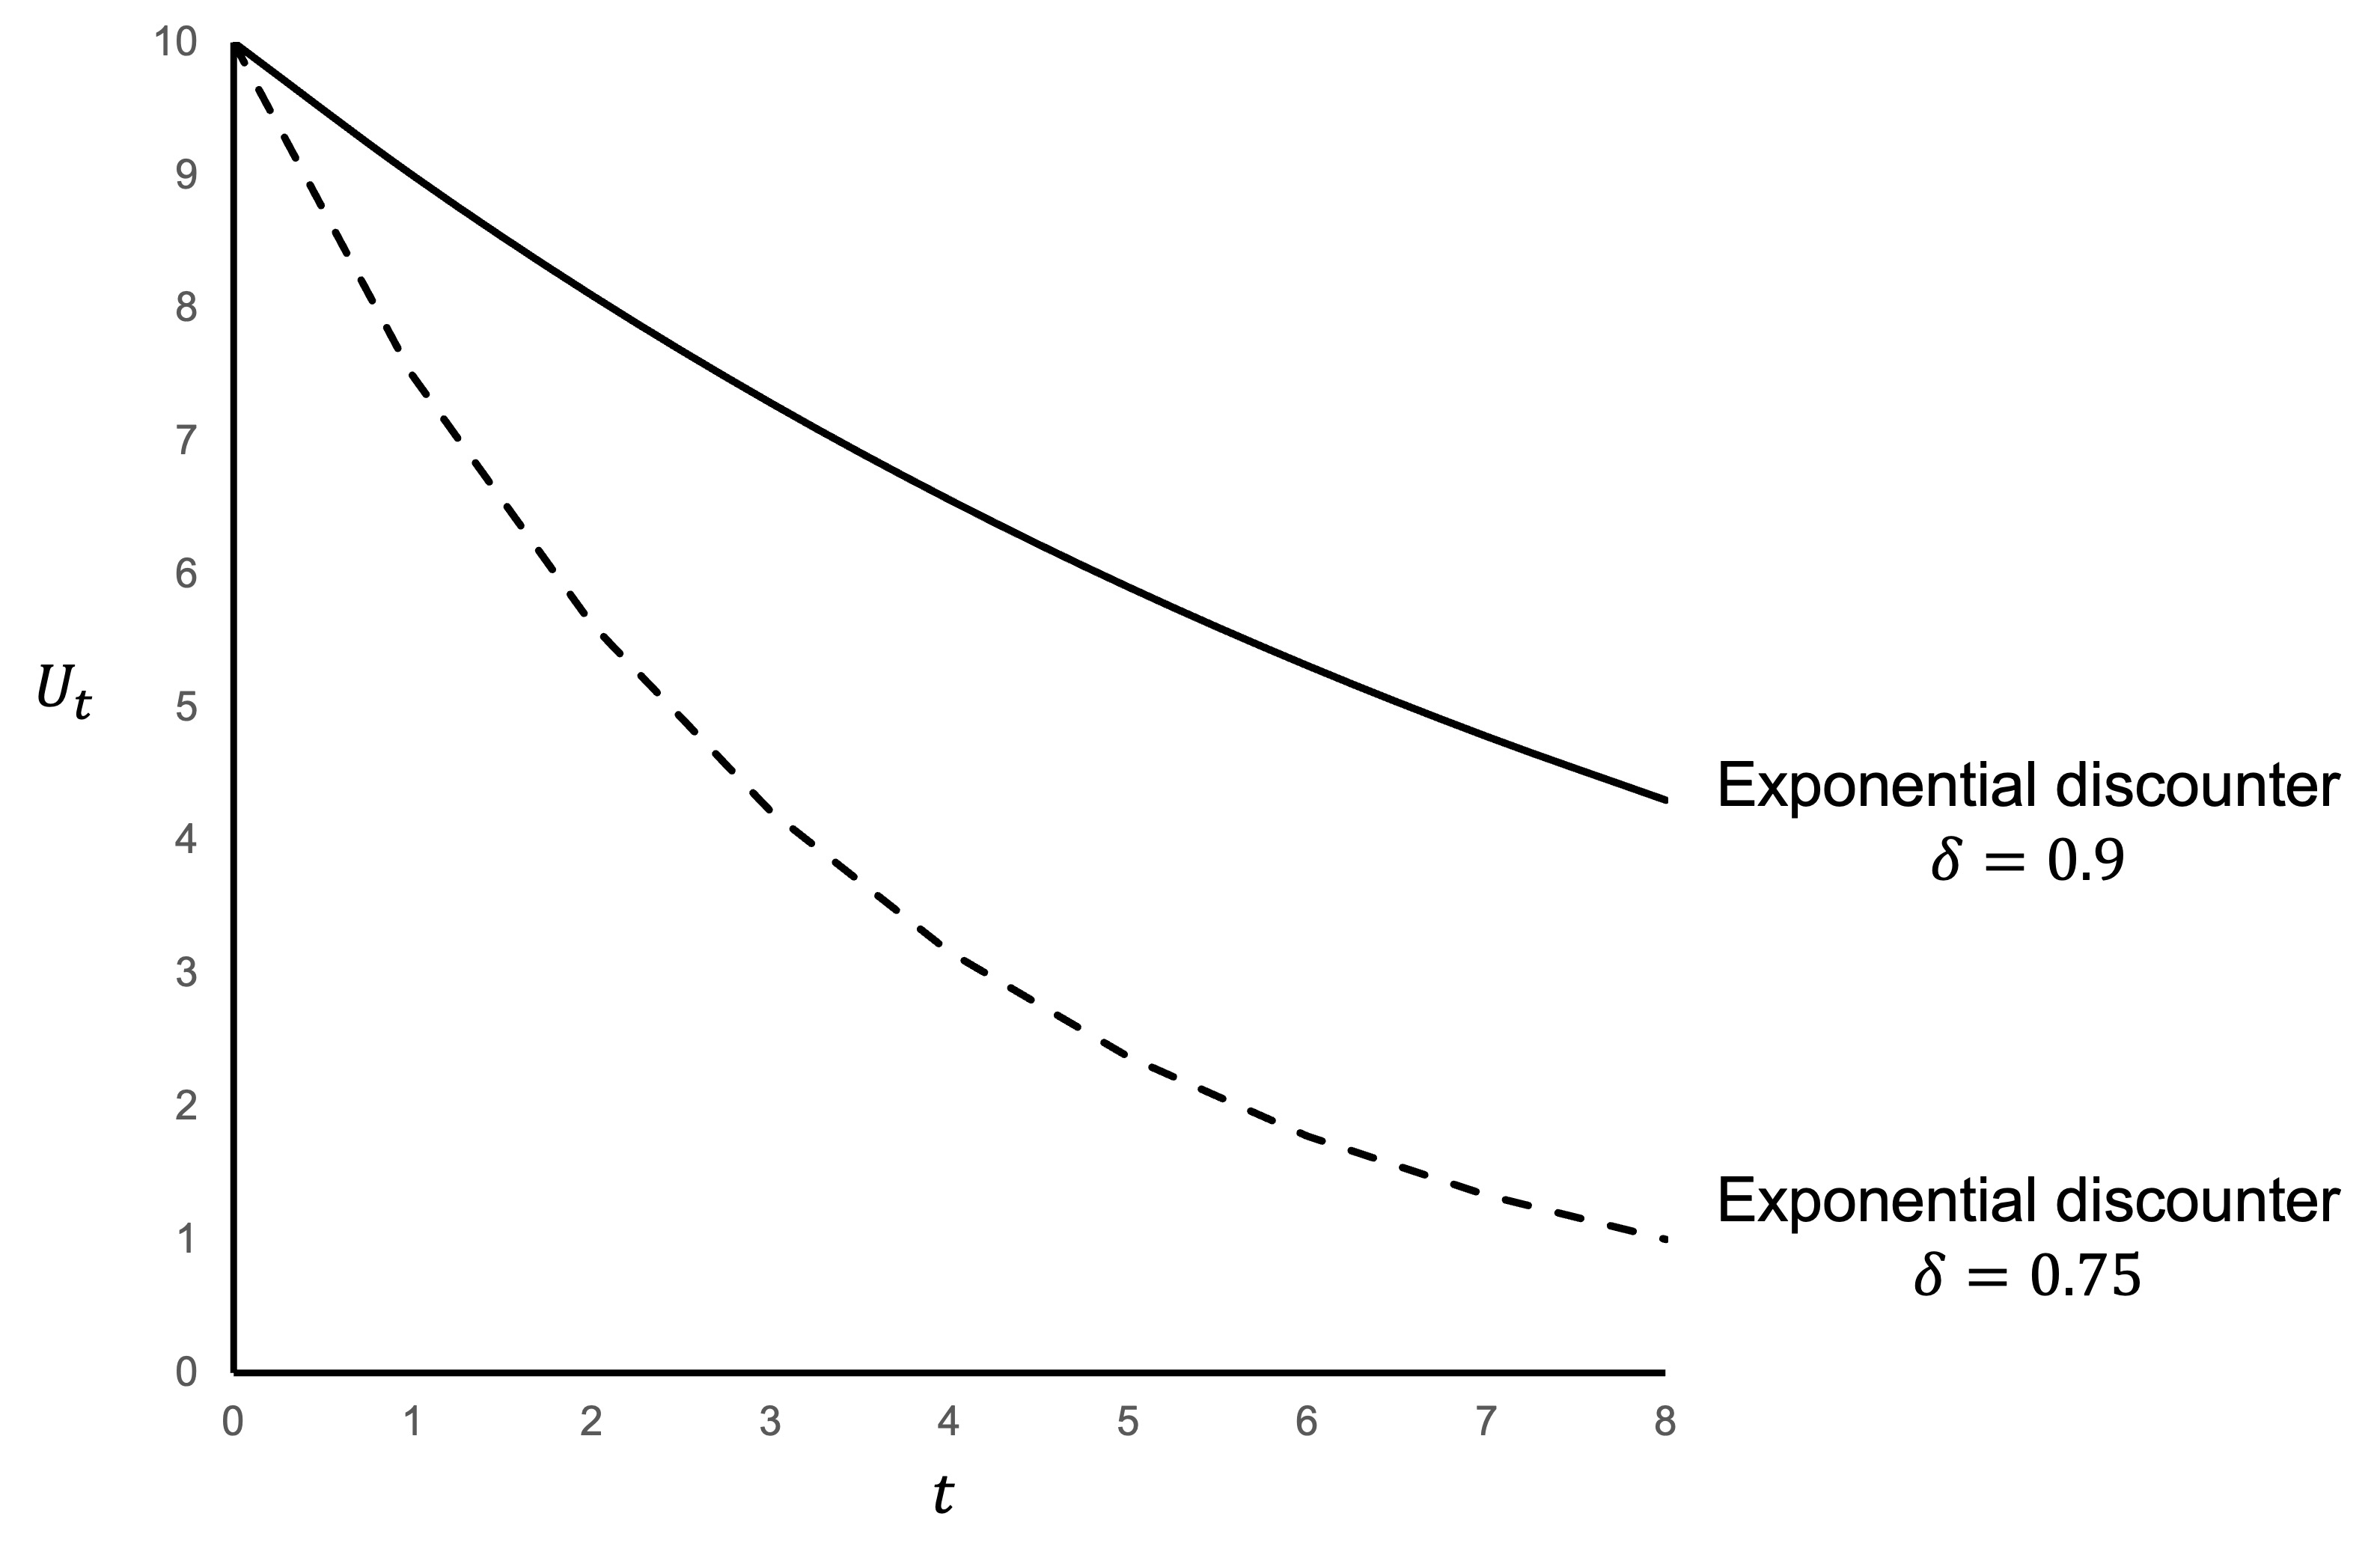
\includegraphics{intertemporal-choice/img/exponential-discounting.jpg}

}

\caption{\label{fig-exponential}Exponential discount curves}

\end{figure}

\hypertarget{exponential-discounting-examples}{%
\chapter{Exponential discounting
examples}\label{exponential-discounting-examples}}

\hypertarget{example-1-2}{%
\section{Example 1}\label{example-1-2}}

Suppose we have an exponential discounter with \(\delta=0.95\) and
utility each period of \(u(x_n)=x_n\).

Choice 1: Would this agent prefer \$100 today (\(t=0\)) or \$110 next
week (\(t=1\))?

\begin{align*}
U_0(0,\$100)&=u(\$100) \\
&=100 \\
\\
U_0(1,\$110)&=\delta u(\$110) \\
&=0.95*110 \\
&=104.50
\end{align*}

The exponential discounter will prefer to receive \$110 next week.

Choice 2: Would this agent prefer \$100 next week (\(t=1\)) or \$110 in
two weeks (\(t=2\))?

\begin{align*}
U_1(1,\$100)&=\delta u(\$110) \\
&=0.95*100 \\
&=95 \\
\\
U_1(2,\$110)&=\delta^2 u(\$110) \\
&=0.95^2*110 \\
&=99.275
\end{align*}

The exponential discounter will prefer to receive \$110 in two weeks.
The set of decisions across Choice 1 and Choice 2 are time consistent.
If the agent selected \$110 in two weeks for Choice 2 and was given a
chance to change their choice after one week (which is effectively
Choice 1), they would not change.

Figure~\ref{fig-example_1} visualises the effect of discounting in
Choice 2.

The two bars represent the options: \$100 at \(t=1\) and \$110 at
\(t=2\). The line from each represents the discounted value of that
option at each time. For example, at \(t=1\) the discounted utility of
the \$100 received at \(t=1\) is \$100 and of the \$110 received at
\(t=2\) is \$104.50. We can read those values from the line. For any
time \(t\) we can determine which option would be preferred by seeing
which line is higher.

\begin{figure}

{\centering 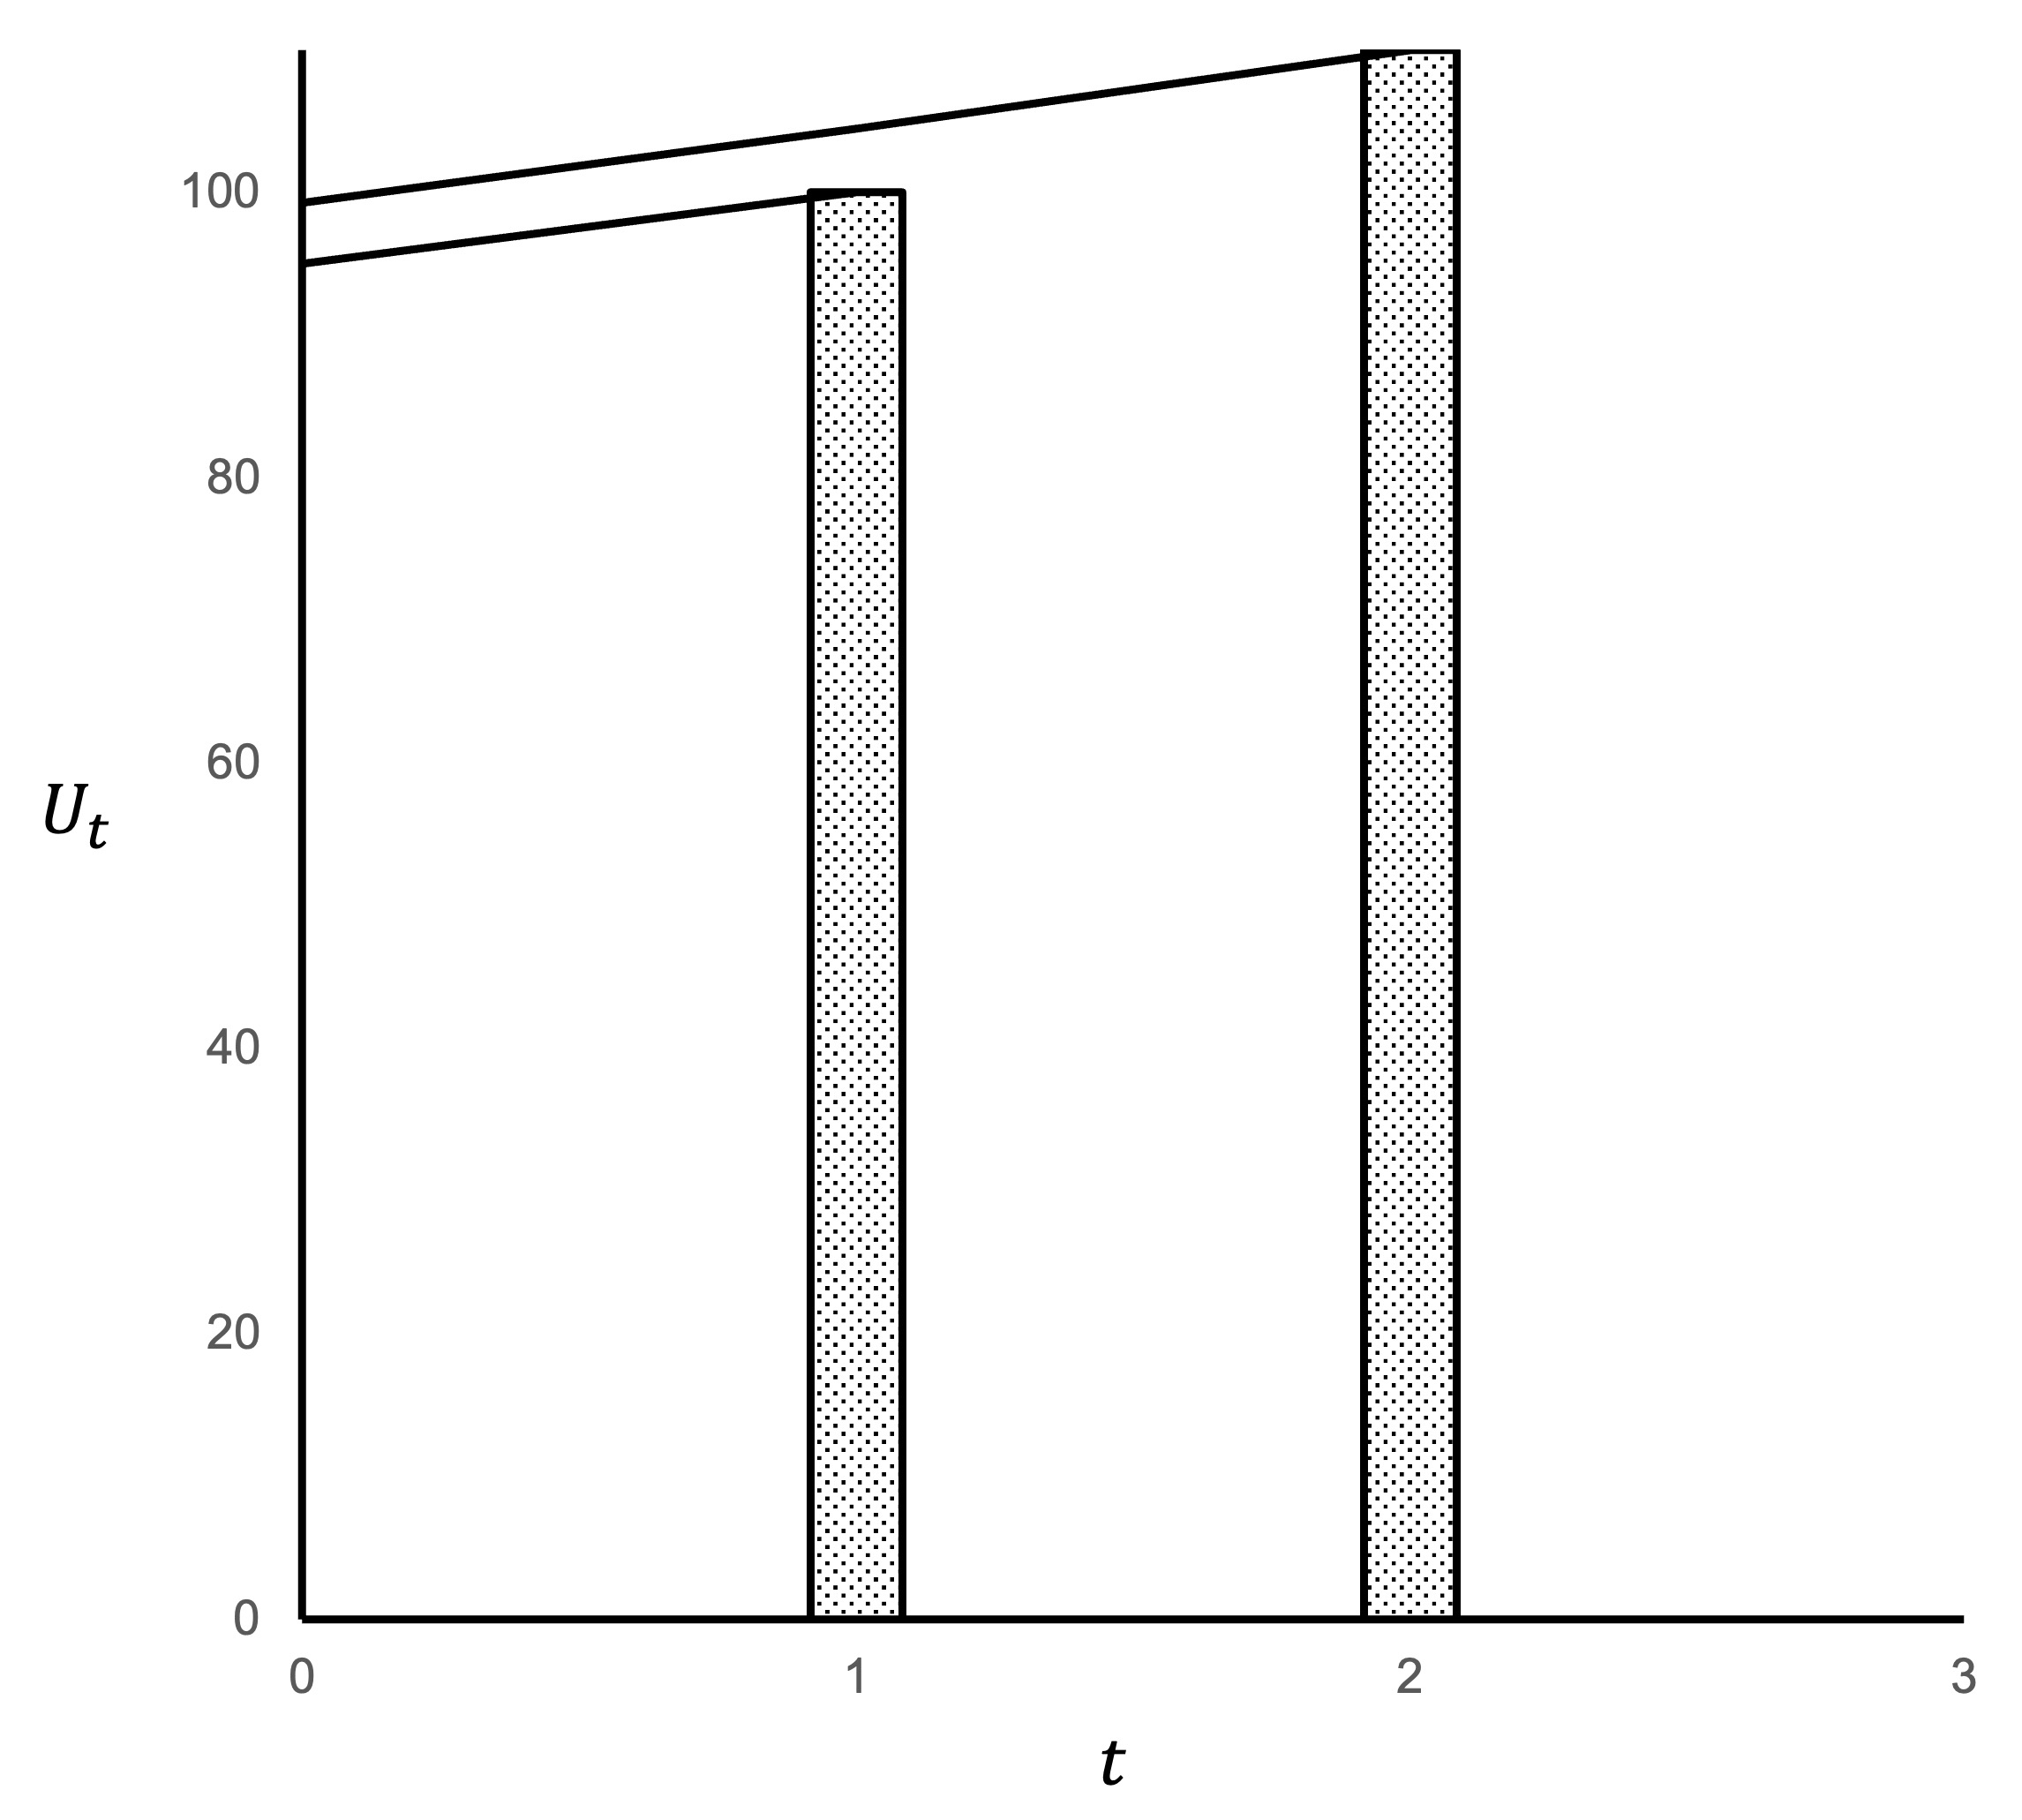
\includegraphics[width=0.6\textwidth,height=\textheight]{intertemporal-choice/img/example_1.jpg}

}

\caption{\label{fig-example_1}Choice 2}

\end{figure}

You will note that the two lines do not cross. For an exponential
discounter, if one line is higher at any particular time \(t\), it is
higher at all times.

Figure~\ref{fig-example_1a} visualises Choice 1.

\begin{figure}

{\centering 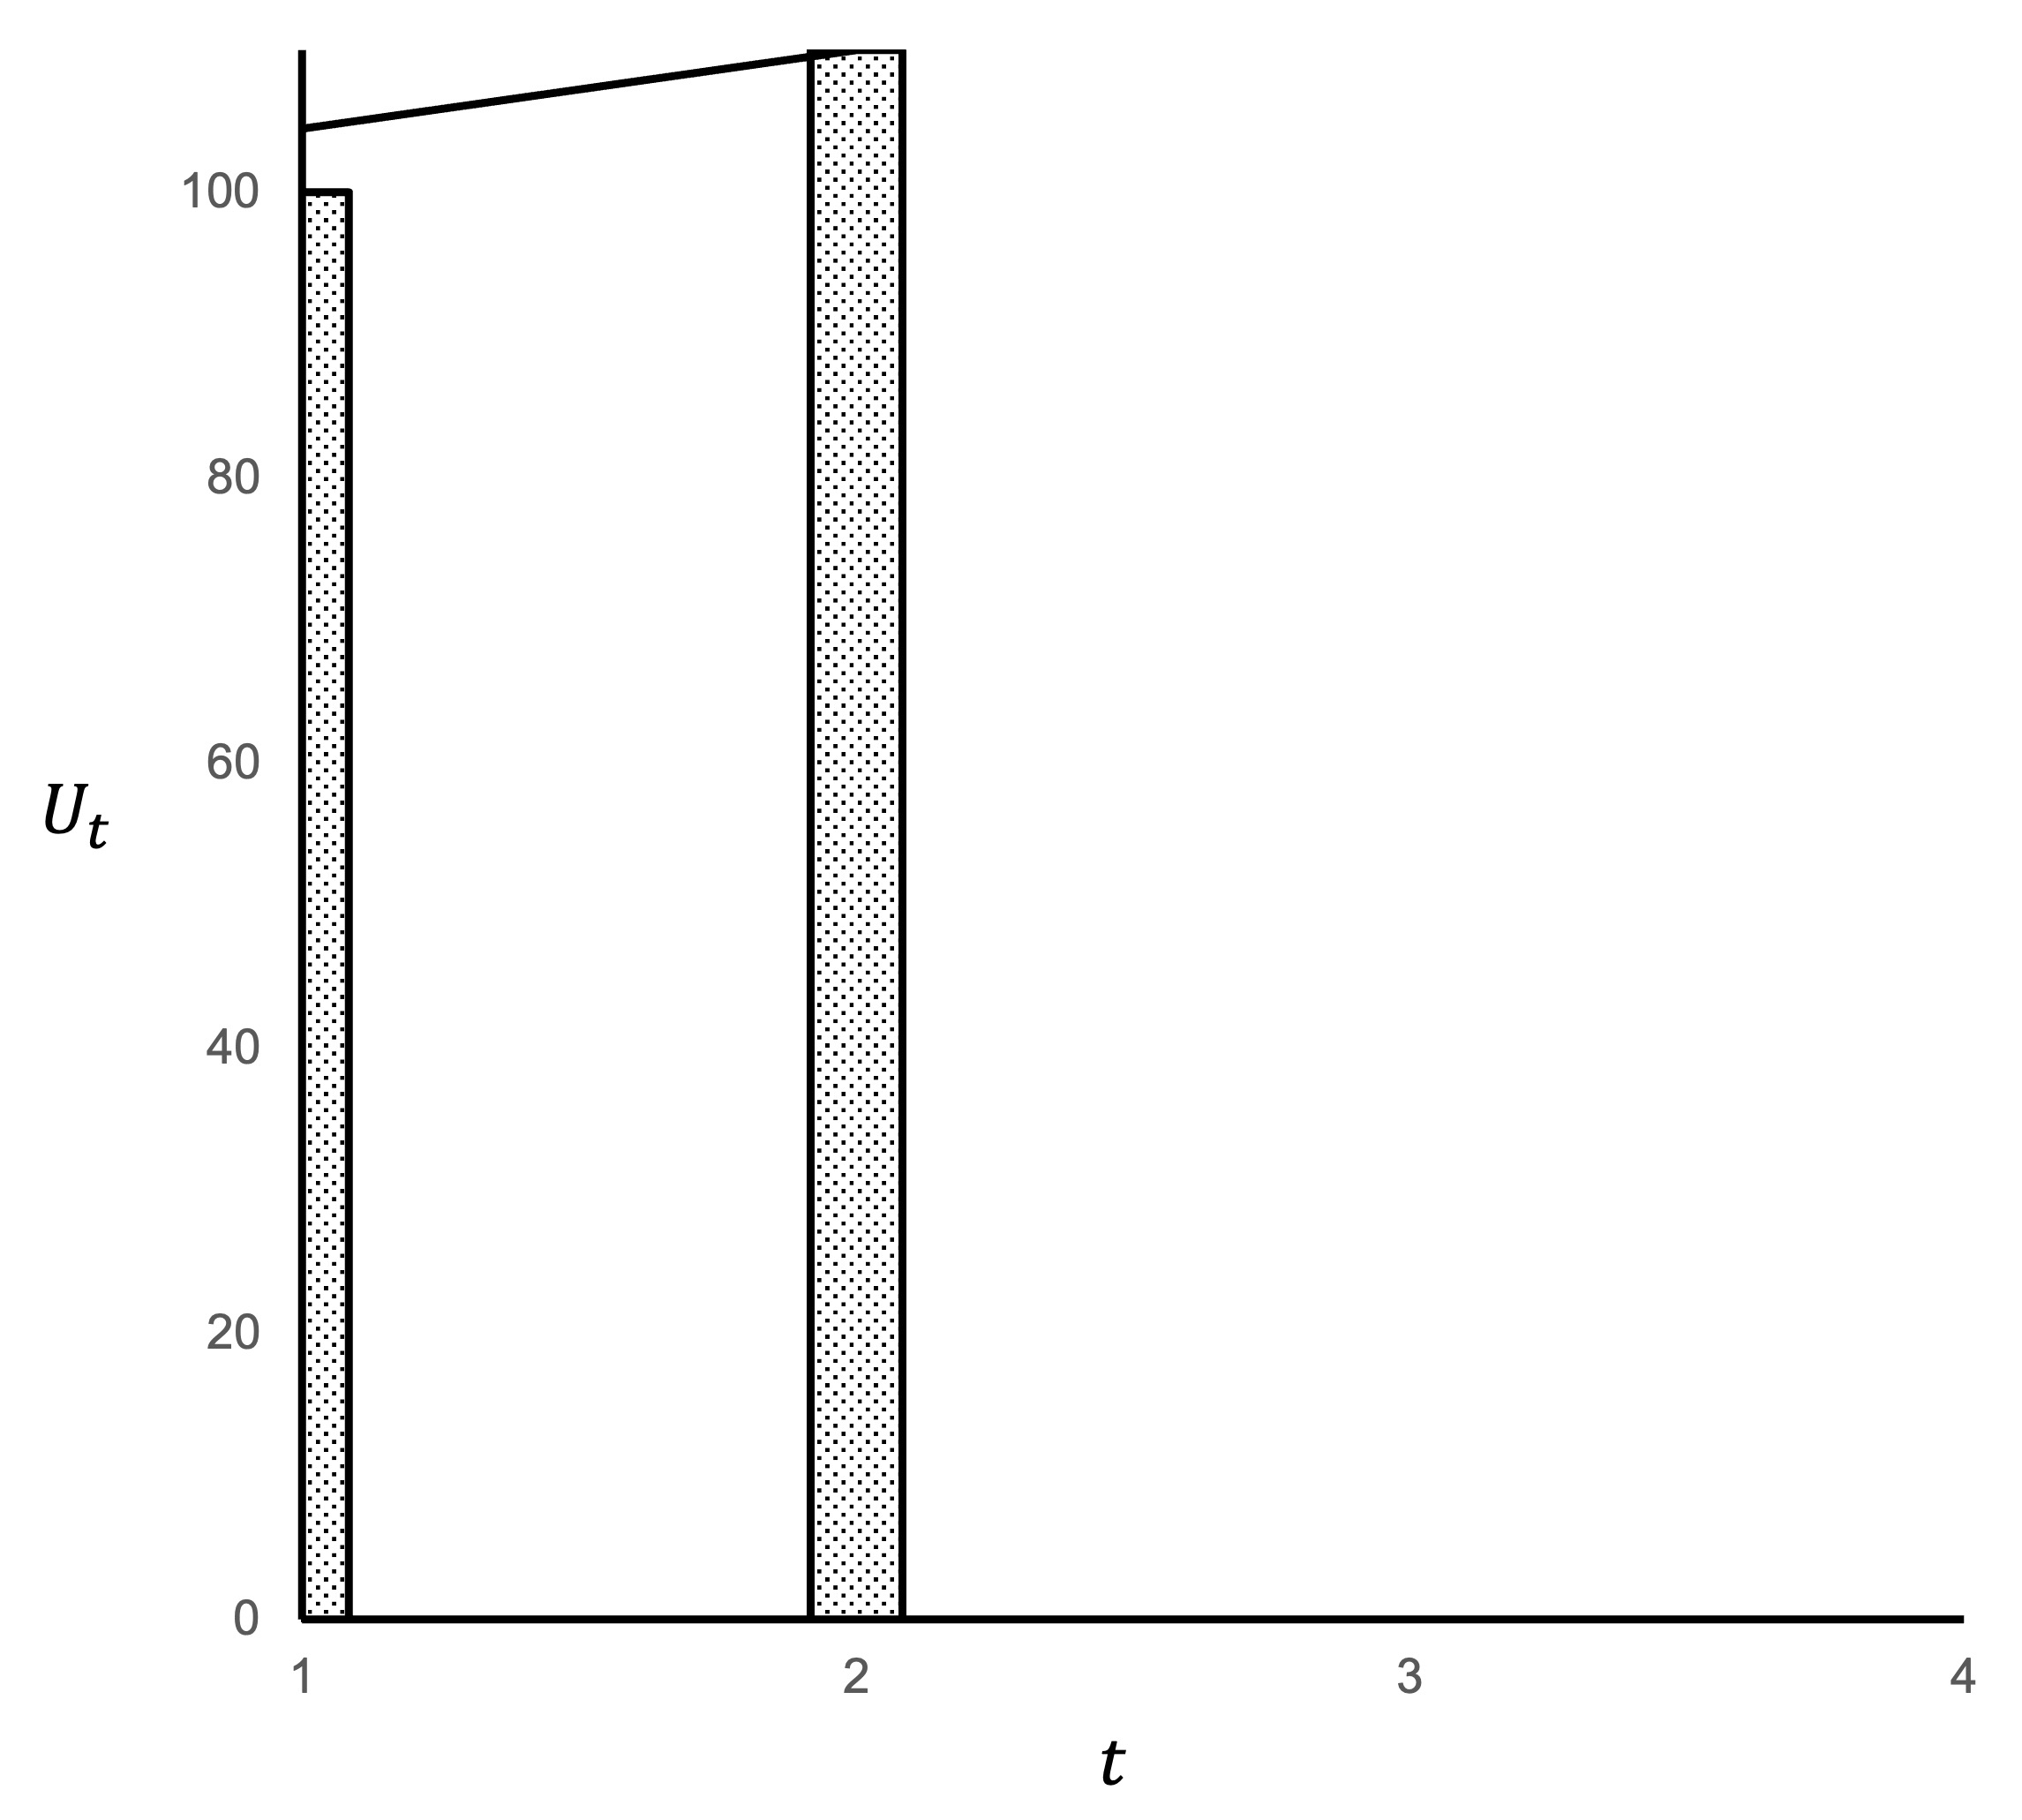
\includegraphics[width=0.6\textwidth,height=\textheight]{intertemporal-choice/img/example_1a.jpg}

}

\caption{\label{fig-example_1a}Choice 1}

\end{figure}

\hypertarget{example-2-2}{%
\section{Example 2}\label{example-2-2}}

Suppose we have an exponential discounter with \(\delta=0.95\) per week
and utility each period of \(u(x_n)=x_n\)

They are offered \$100 today. What sum would they need to be offered in
one year (52 weeks) to prefer that later payment to the \$100 today?

\begin{align*}
U_0(0,\$100)&=u(\$100) \\
&=100 \\
\\
U_0(52,\$x)&=\delta^{52} u(\$x) \\
&=0.95^{52}*x
\end{align*}

They will prefer \$\(x\) in 52 weeks if \(U(\$x \text{ at } t=52)\) is
greater than 100.

\begin{align*}
0.95^{52}*x&>100 \\[6pt]
x&>\frac{100}{0.95^{52}} \\[6pt]
x&>\$1440.03
\end{align*}

The agent would be willing to wait a year for payment if they were paid
more than \$1440.03.

Figure~\ref{fig-example_2} visualises this problem.

\begin{figure}

{\centering 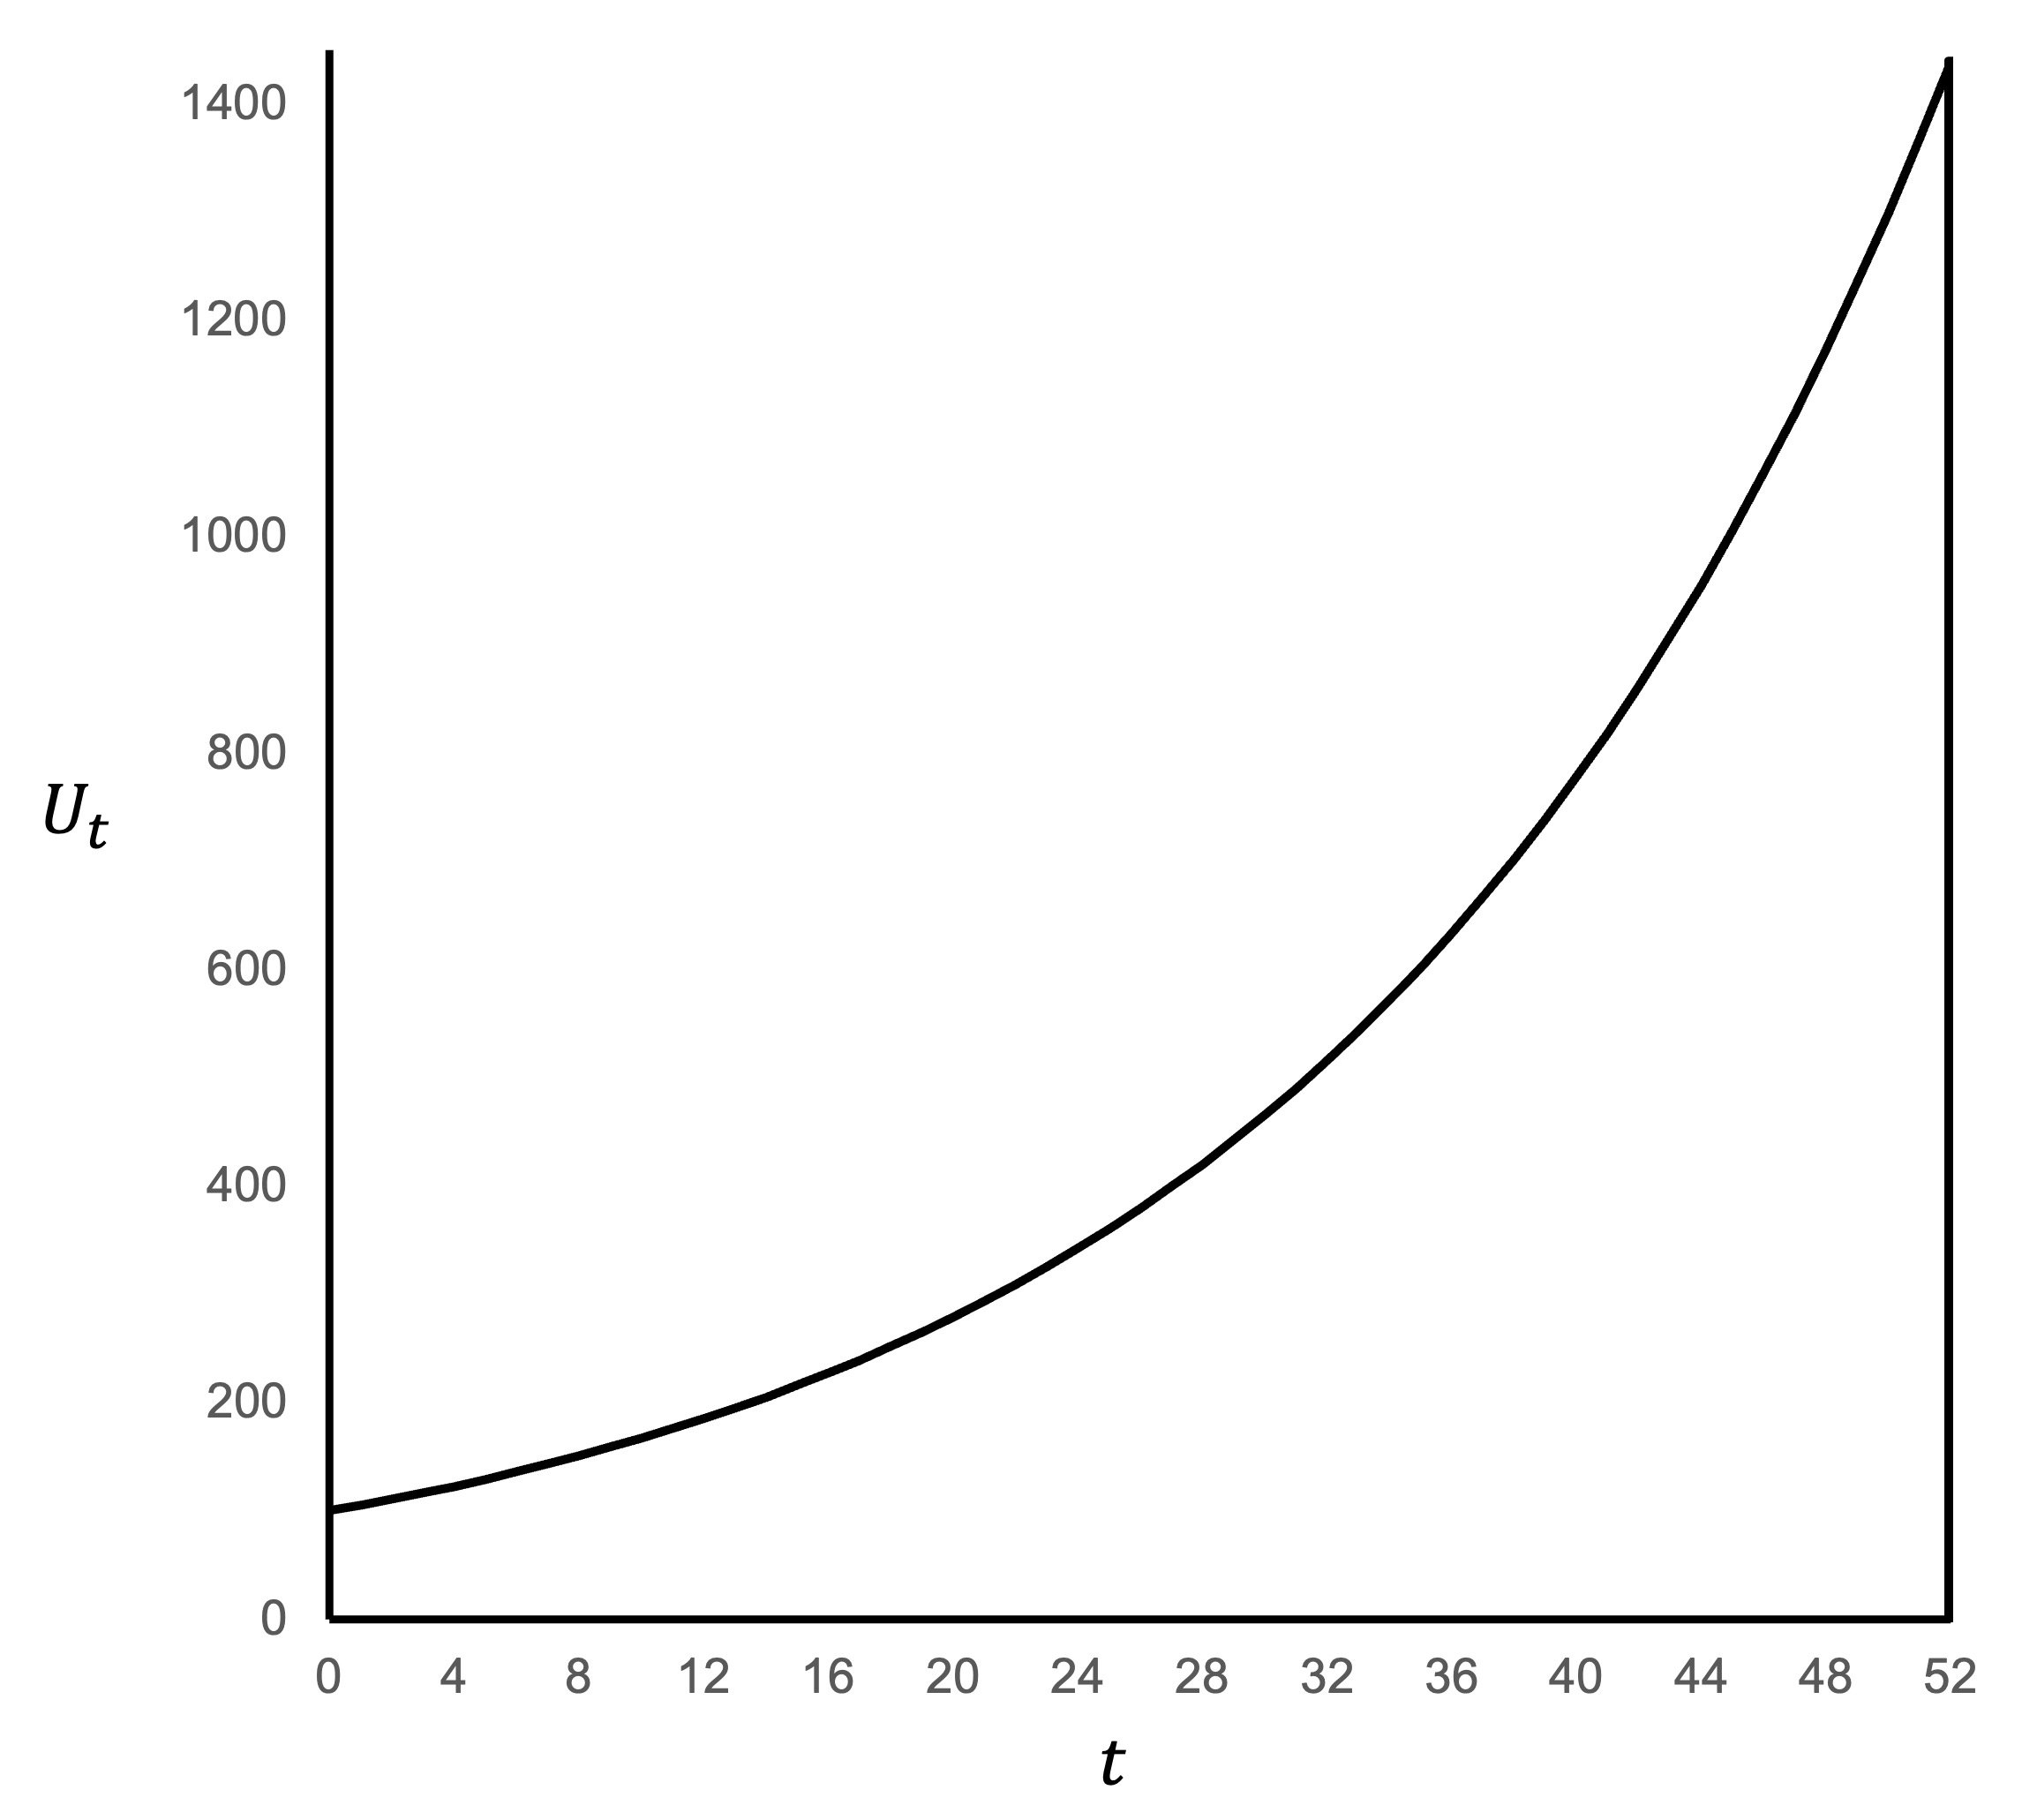
\includegraphics[width=0.6\textwidth,height=\textheight]{intertemporal-choice/img/example_2.jpg}

}

\caption{\label{fig-example_2}Example 2}

\end{figure}

\hypertarget{example-3-1}{%
\section{Example 3}\label{example-3-1}}

Suppose we have an exponential discounter with \(\delta=0.75\) and
utility each period of \(u(x_n)=x_n\).

Would this agent prefer \$10 in five days (\(t=5\)) or \$20 in 10 days
(\(t=10\))?

\begin{align*}
U_0(5,\$10)&=\delta^5u(\$10) \\
&=0.75^5\times 10 \\
&=2.373 \\
\\
U_0(10,\$20)&=\delta^{10} u(\$20) \\
&=0.75^{10}\times 20 \\
&=1.126
\end{align*}

This exponential discounter will prefer to receive \$10 in five days.

What if their discount rate was \(\delta=0.95\)?

\begin{align*}
U_0(5,\$10)&=\delta^5u(\$10) \\
&=0.95^5\times 10 \\
&=7.738 \\
\\
U_0(10,\$20)&=\delta^{10} u(\$20) \\
&=0.95^{10}\times 20 \\
&=11.975
\end{align*}

This exponential discounter will prefer to receive \$20 in 10 days.

\begin{figure}

\begin{minipage}[t]{0.50\linewidth}

{\centering 

\raisebox{-\height}{

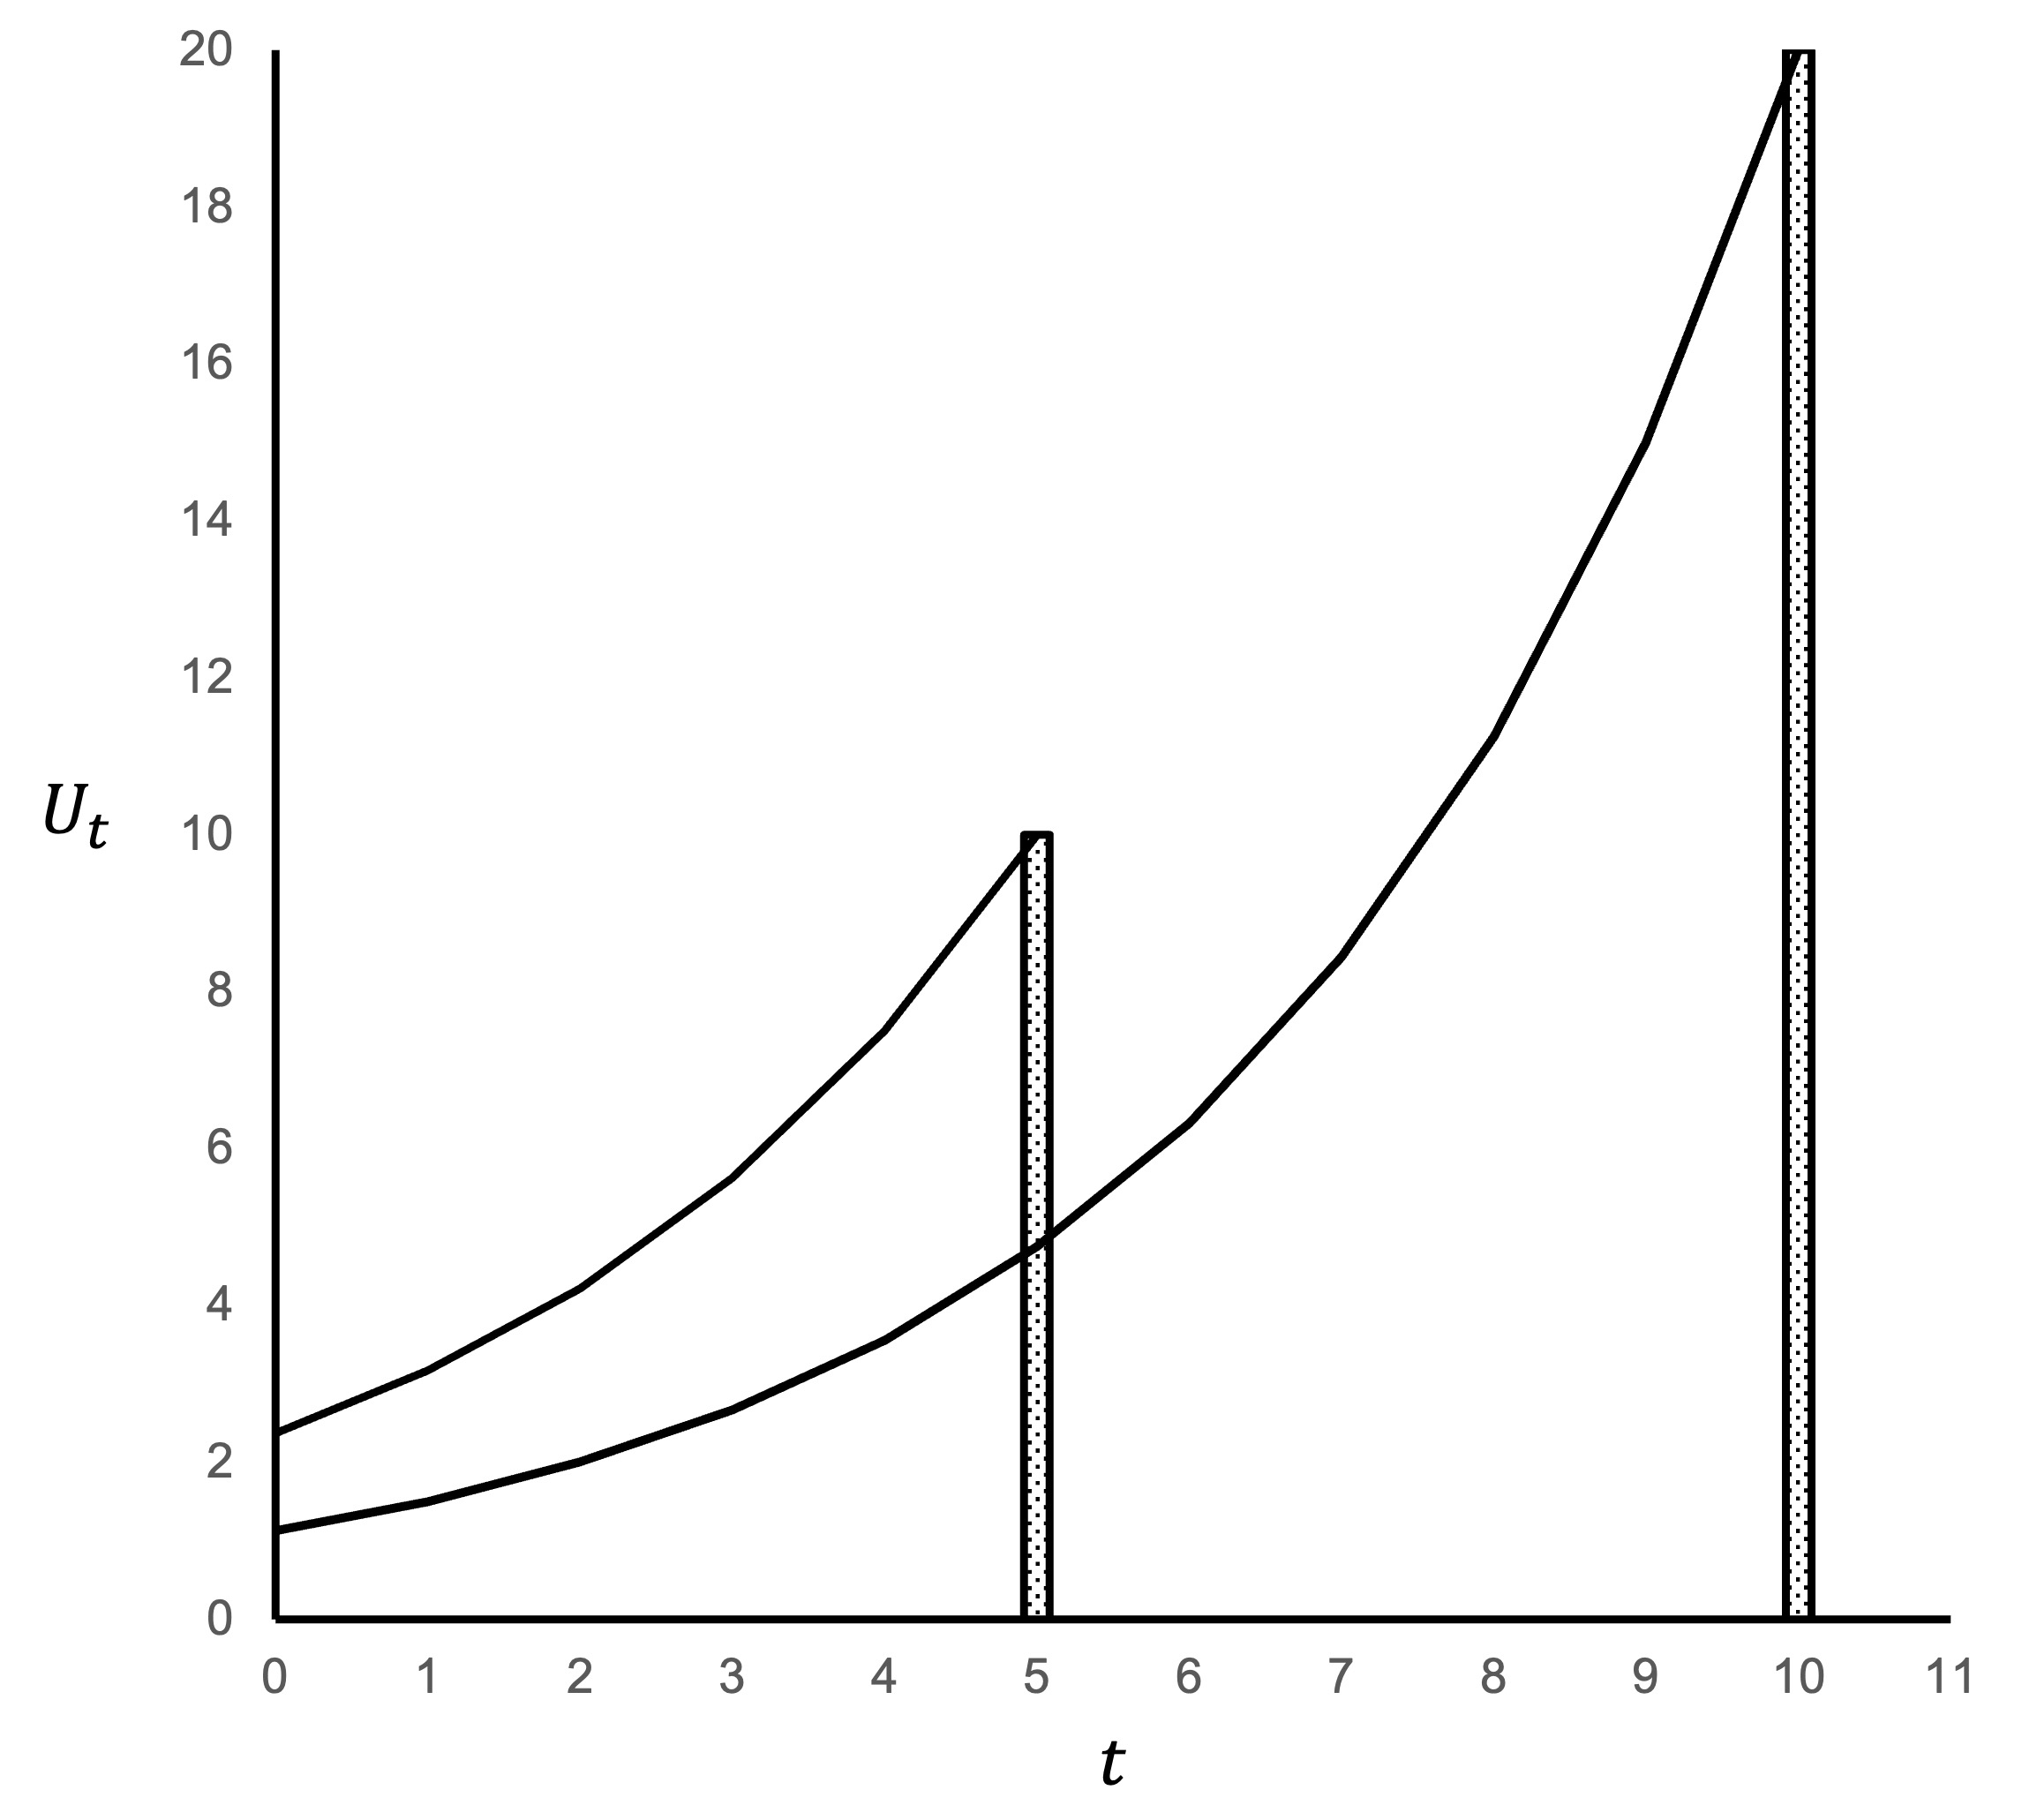
\includegraphics{intertemporal-choice/img/example_3.jpg}

}

}

\subcaption{\label{fig-example_3}\(\delta=0.75\)}
\end{minipage}%
%
\begin{minipage}[t]{0.50\linewidth}

{\centering 

\raisebox{-\height}{

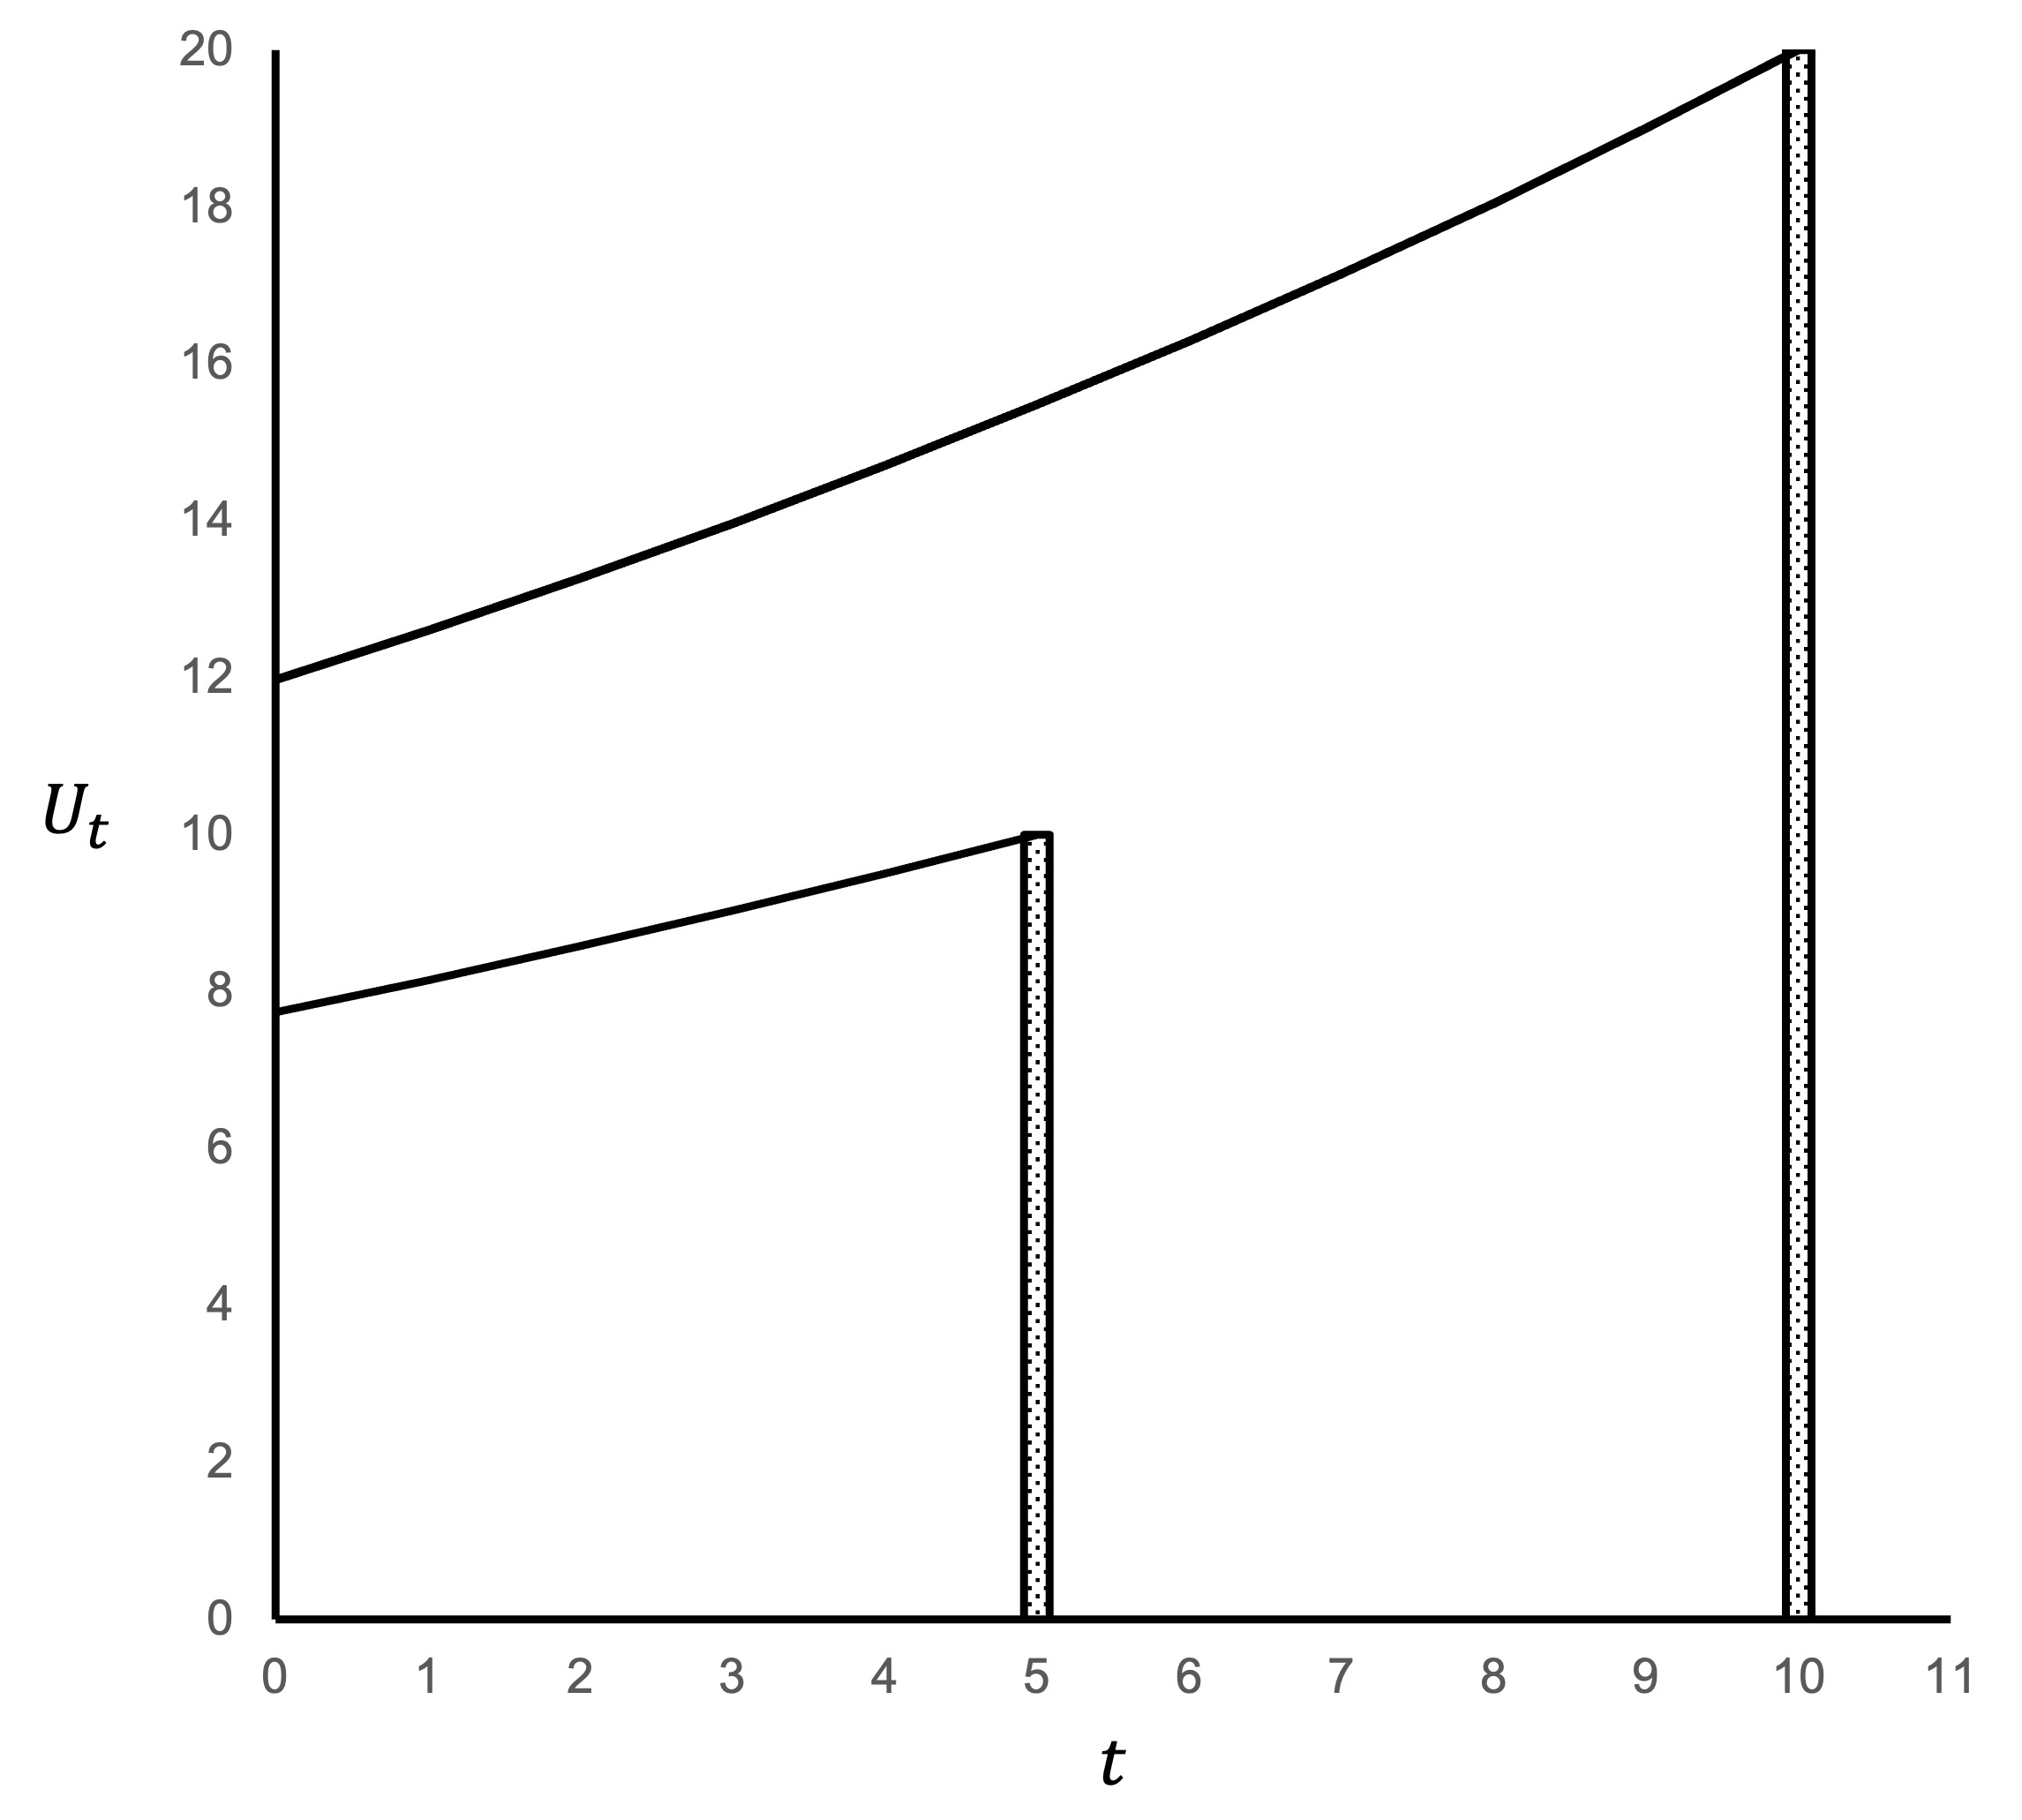
\includegraphics{intertemporal-choice/img/example_3a.jpg}

}

}

\subcaption{\label{fig-example_3a}\(\delta=0.95\)}
\end{minipage}%

\caption{\label{fig-exponential}Exponential discounting}

\end{figure}

\hypertarget{exponential-discounting-anomalies}{%
\chapter{Exponential discounting
anomalies}\label{exponential-discounting-anomalies}}

\hypertarget{estimation-of-delta}{%
\section{\texorpdfstring{Estimation of
\(\delta\)}{Estimation of \textbackslash delta}}\label{estimation-of-delta}}

Frederick et al. (2002) plotted estimates of 𝛿 from a set of published
papers. Figure 1a shows that the estimated discount factor increases
with time horizon. If studies with horizons of one year or less are
excluded, there is no relationship between the discount factor and time
horizon (Figure 1b).

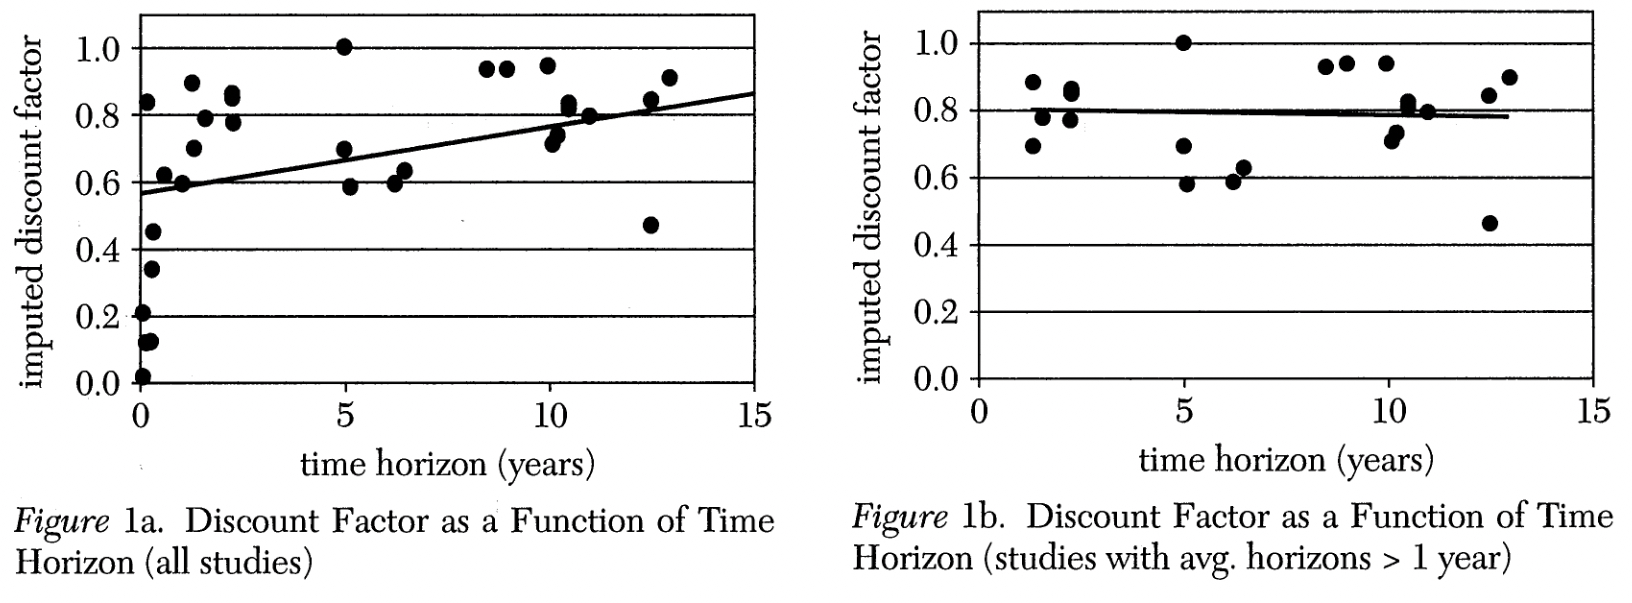
\includegraphics{intertemporal-choice/img/Frederick_at_al_2002_Figure_1.jpg}

R. Thaler (1981) estimated the discount rate of experimental subjects by
presenting them with a choice between a prize today or a larger later.
In each case, they were asked, given the size of the prize that could be
received today, how large would the future prize would need to be such
that waiting would be as attractive as receiving the money now.

For example, some subjects were asked how large a future prize would
need to be such that they would be happy to wait three months, one year
or three years rather than receiving \$15 today. The median answers were
\$30, \$60 and \$100 respectively. If you use these estimates to
calculate an implied discount rate, the result is 277\%, 139\% and 63\%.
It can be seen that this discount rate is decreasing with the length of
delay (which matches the pattern of increasing discount factor with
length of delay).

\hypertarget{preference-reversal}{%
\section{Preference reversal}\label{preference-reversal}}

Green et al. (1994) offered experimental subjects choices between a
smaller reward and delayed larger reward while varying the delay. For
example, they offered:

\begin{itemize}
\item
  \$20 now or \$50 in three months
\item
  \$20 in one week or \$50 in three months and one week.
\end{itemize}

Across the choices offered to the experimental subjects, there was a
consistent effect whereby incrementing the delay for both rewards
equally would result in a switch from the small sooner reward to the
latter larger reward.

In a study by Kirby and Herrnstein (1995), 34 of 36 experimental
subjects reversed preference from a larger later reward to a smaller
earlier reward as the delays to both decreased.

\hypertarget{healthy-choices}{%
\subsection{Healthy choices}\label{healthy-choices}}

Read and Leeuwen (1998) asked 200 study participants to make a choice
between healthy or unhealthy snacks (e.g., banana or apple versus Mars
bar or Snickers bar) that they would receive in one week. 48\% of men
and 51\% of women chose the healthy choice.

At the scheduled time one week later they asked the participants to
choose again. Although no reference was made to their previous choice,
this effectively gave them the opportunity to change their mind. This
time, only 25\% of men and 11\% of women chose the healthy snack. While
many changed from the healthy to unhealthy snack, almost no-one changed
from the unhealthy to healthy snack.

This result is evidence of time inconsistency. The participants made
different decisions depending upon when they made the decision.

\hypertarget{present-bias}{%
\chapter{Present bias}\label{present-bias}}

Present bias occurs when we place additional weight on costs and
benefits at the present time.

\hypertarget{the-betadelta-model}{%
\section{\texorpdfstring{The \(\beta\delta\)
model}{The \textbackslash beta\textbackslash delta model}}\label{the-betadelta-model}}

One simple model of present bias is the quasi-hyperbolic discounting
model (it is a discrete time version of hyperbolic discounting).

\begin{align*}
U_0&=u(x_0)+\beta \delta u(x_1)+\beta \delta^2 u*(x_2)+ ... + \beta \delta^T u(x_T) \\
&=u(x_0)+\beta \sum_{t=1}^{t=T}\delta^t u(x_t)
\end{align*}

\(0\leq \delta \leq 1\)

\(0\leq \beta \leq 1\)

\(\beta\) is the short-term discount factor: it scales down all future
dates utility.

\(\delta\) is the usual discount factor.

The degree of discounting in this equation evolves over time as 1,
\(\beta\delta\), \(\beta\delta^2\), \(\beta\delta^3\), \(\beta\delta^4\)
and so on. This progression results in a larger discount for the first
period of delay (\(\beta\delta\)) than the degree of discount for each
subsequent period of delay (\(\delta\)). There is a relative weighting
toward the present. Present bias of this nature can result in time
inconsistency, with decisions at one point reversed at another if given
the opportunity.

\hypertarget{assumptions}{%
\section{Assumptions}\label{assumptions}}

Under the \(\beta\delta\) model we are loosening the assumption of time
consistency. An agent may change their initial plan through time.

However, we are maintaining many of the other assumptions that we used
when we examined exponential discounting. We are maintaining the
assumptions of:

\begin{itemize}
\item
  Consumption independence: Utility in period \(t+k\) is independent of
  consumption in any other period. An outcome's utility is unaffected by
  outcomes in prior or future periods.
\item
  Stationary preferences: \(U_t=U_{t+k}\). That is, the utility function
  is stationary across periods, that is: functional form of \(U_t\) =
  functional form of \(U_{t+1}\), \(U_{t+2}\) etc.
\item
  Utility Independence: All that matters is maximizing the sum of
  discounted utilities. Decision makers are assumed to have no
  preference for the distribution of utilities.
\end{itemize}

\hypertarget{visualising-present-bias}{%
\section{Visualising present bias}\label{visualising-present-bias}}

The following figures illustrate the effect of exponential discounting.

Figure~\ref{fig-present_bias} plots the size of the discount as a
function of \(t\) for a present-biased agent with \(\beta=0.75\) and
\(\delta=0.9\). The discount curve for an exponential discounter with
\(\delta=0.9\) is also plotted. The curve for the present-biased agent
has a large drop for the first period of delay. From then on, the
discount is proportionally the same as for the exponential discounter.

\begin{figure}

{\centering 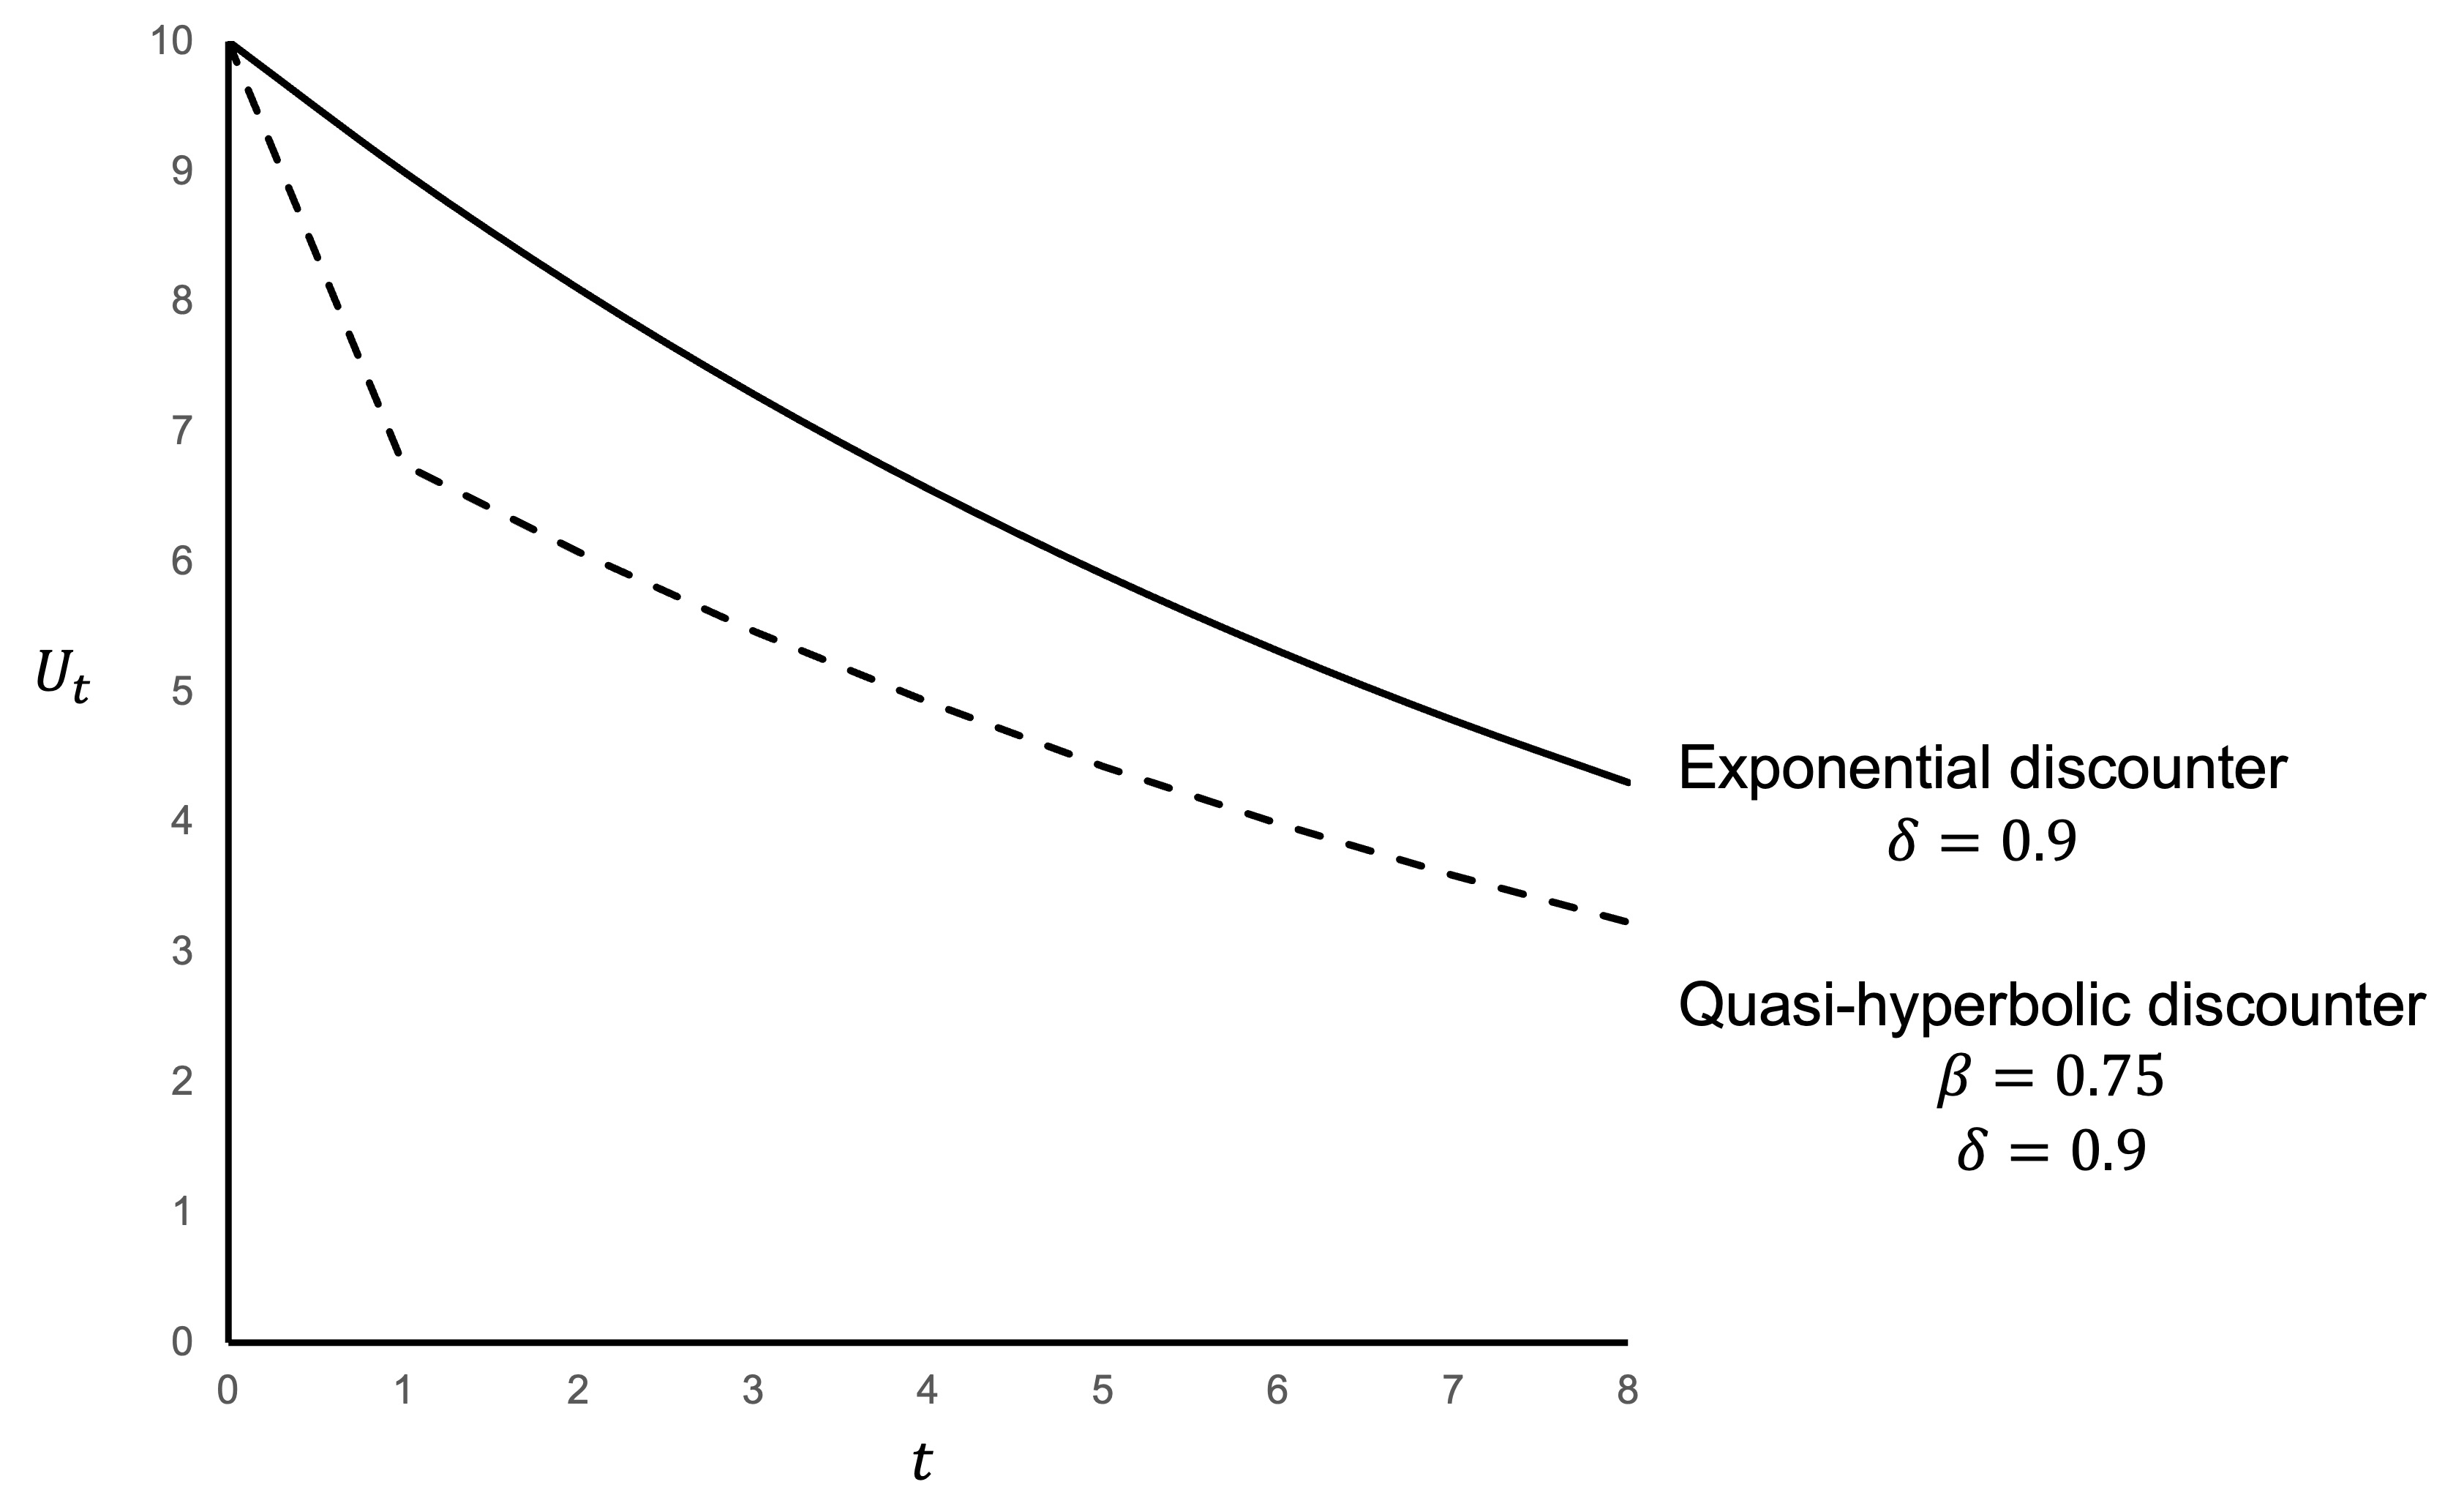
\includegraphics{intertemporal-choice/img/discount-curves.jpg}

}

\caption{\label{fig-present_bias}Discount curves}

\end{figure}

The following two figures illustrate the discount curve for
present-biased and exponential discounting agents with different
parameters.

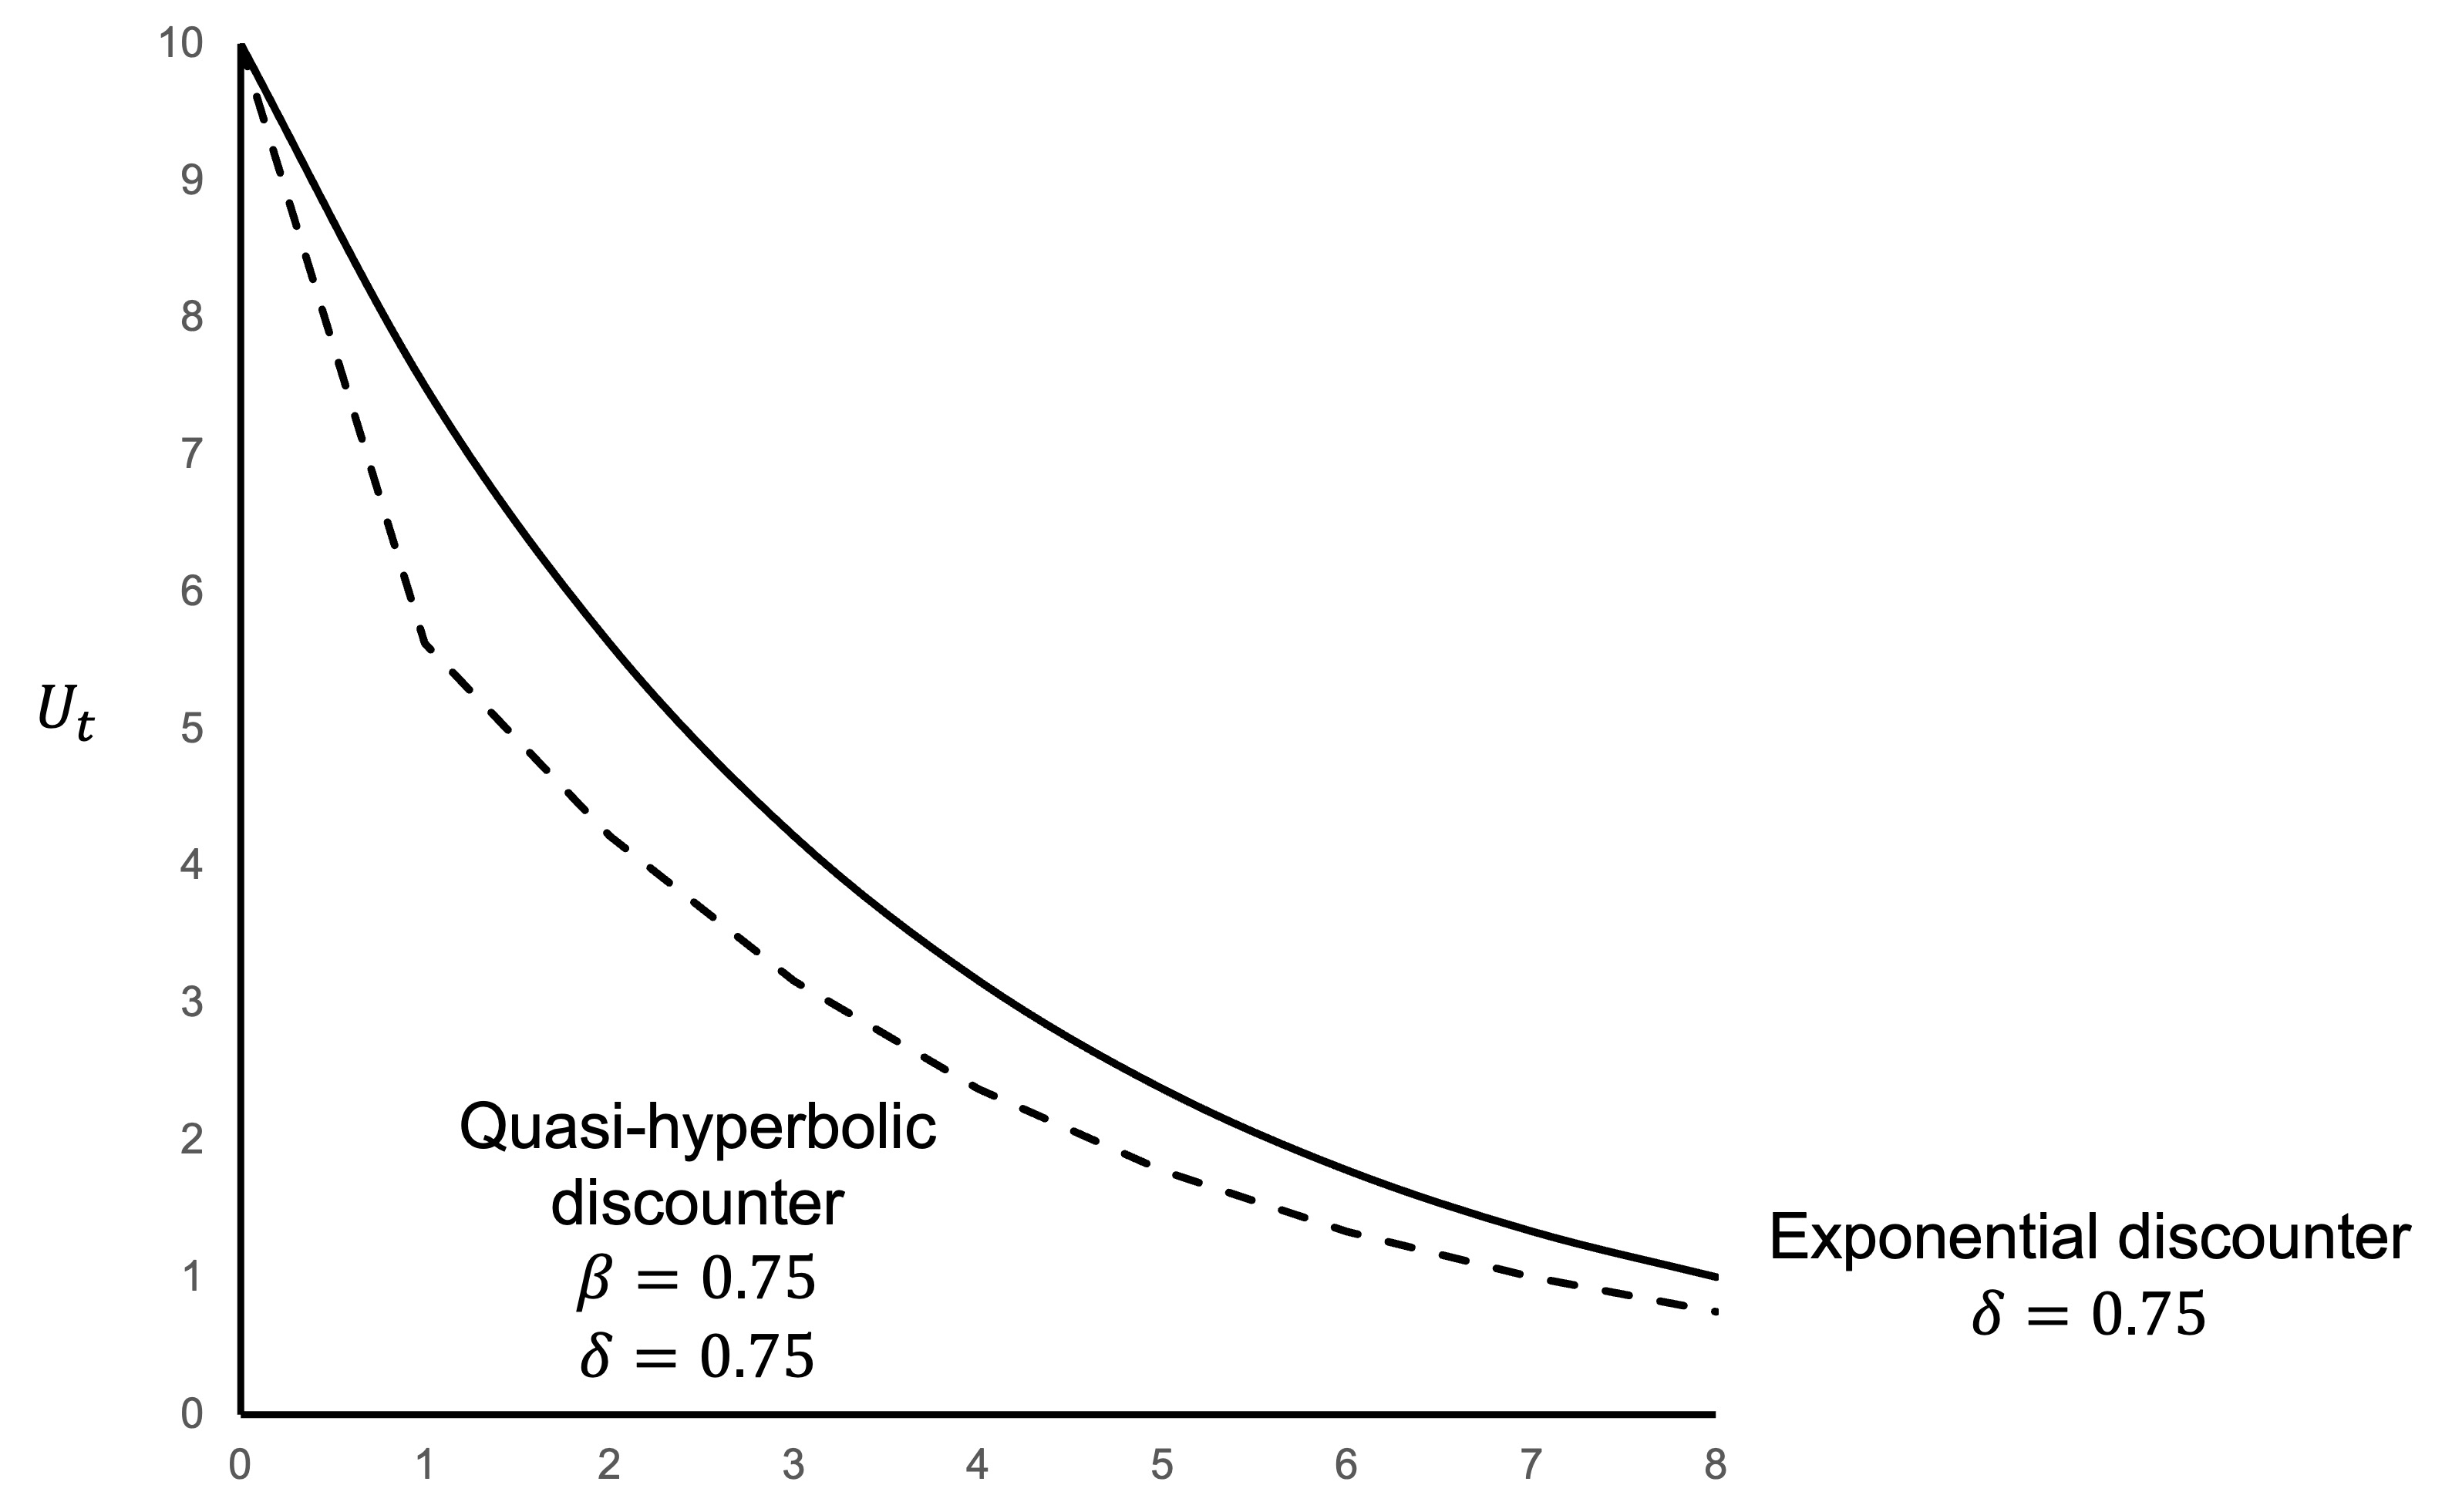
\includegraphics{intertemporal-choice/img/discount-curves-1.jpg}

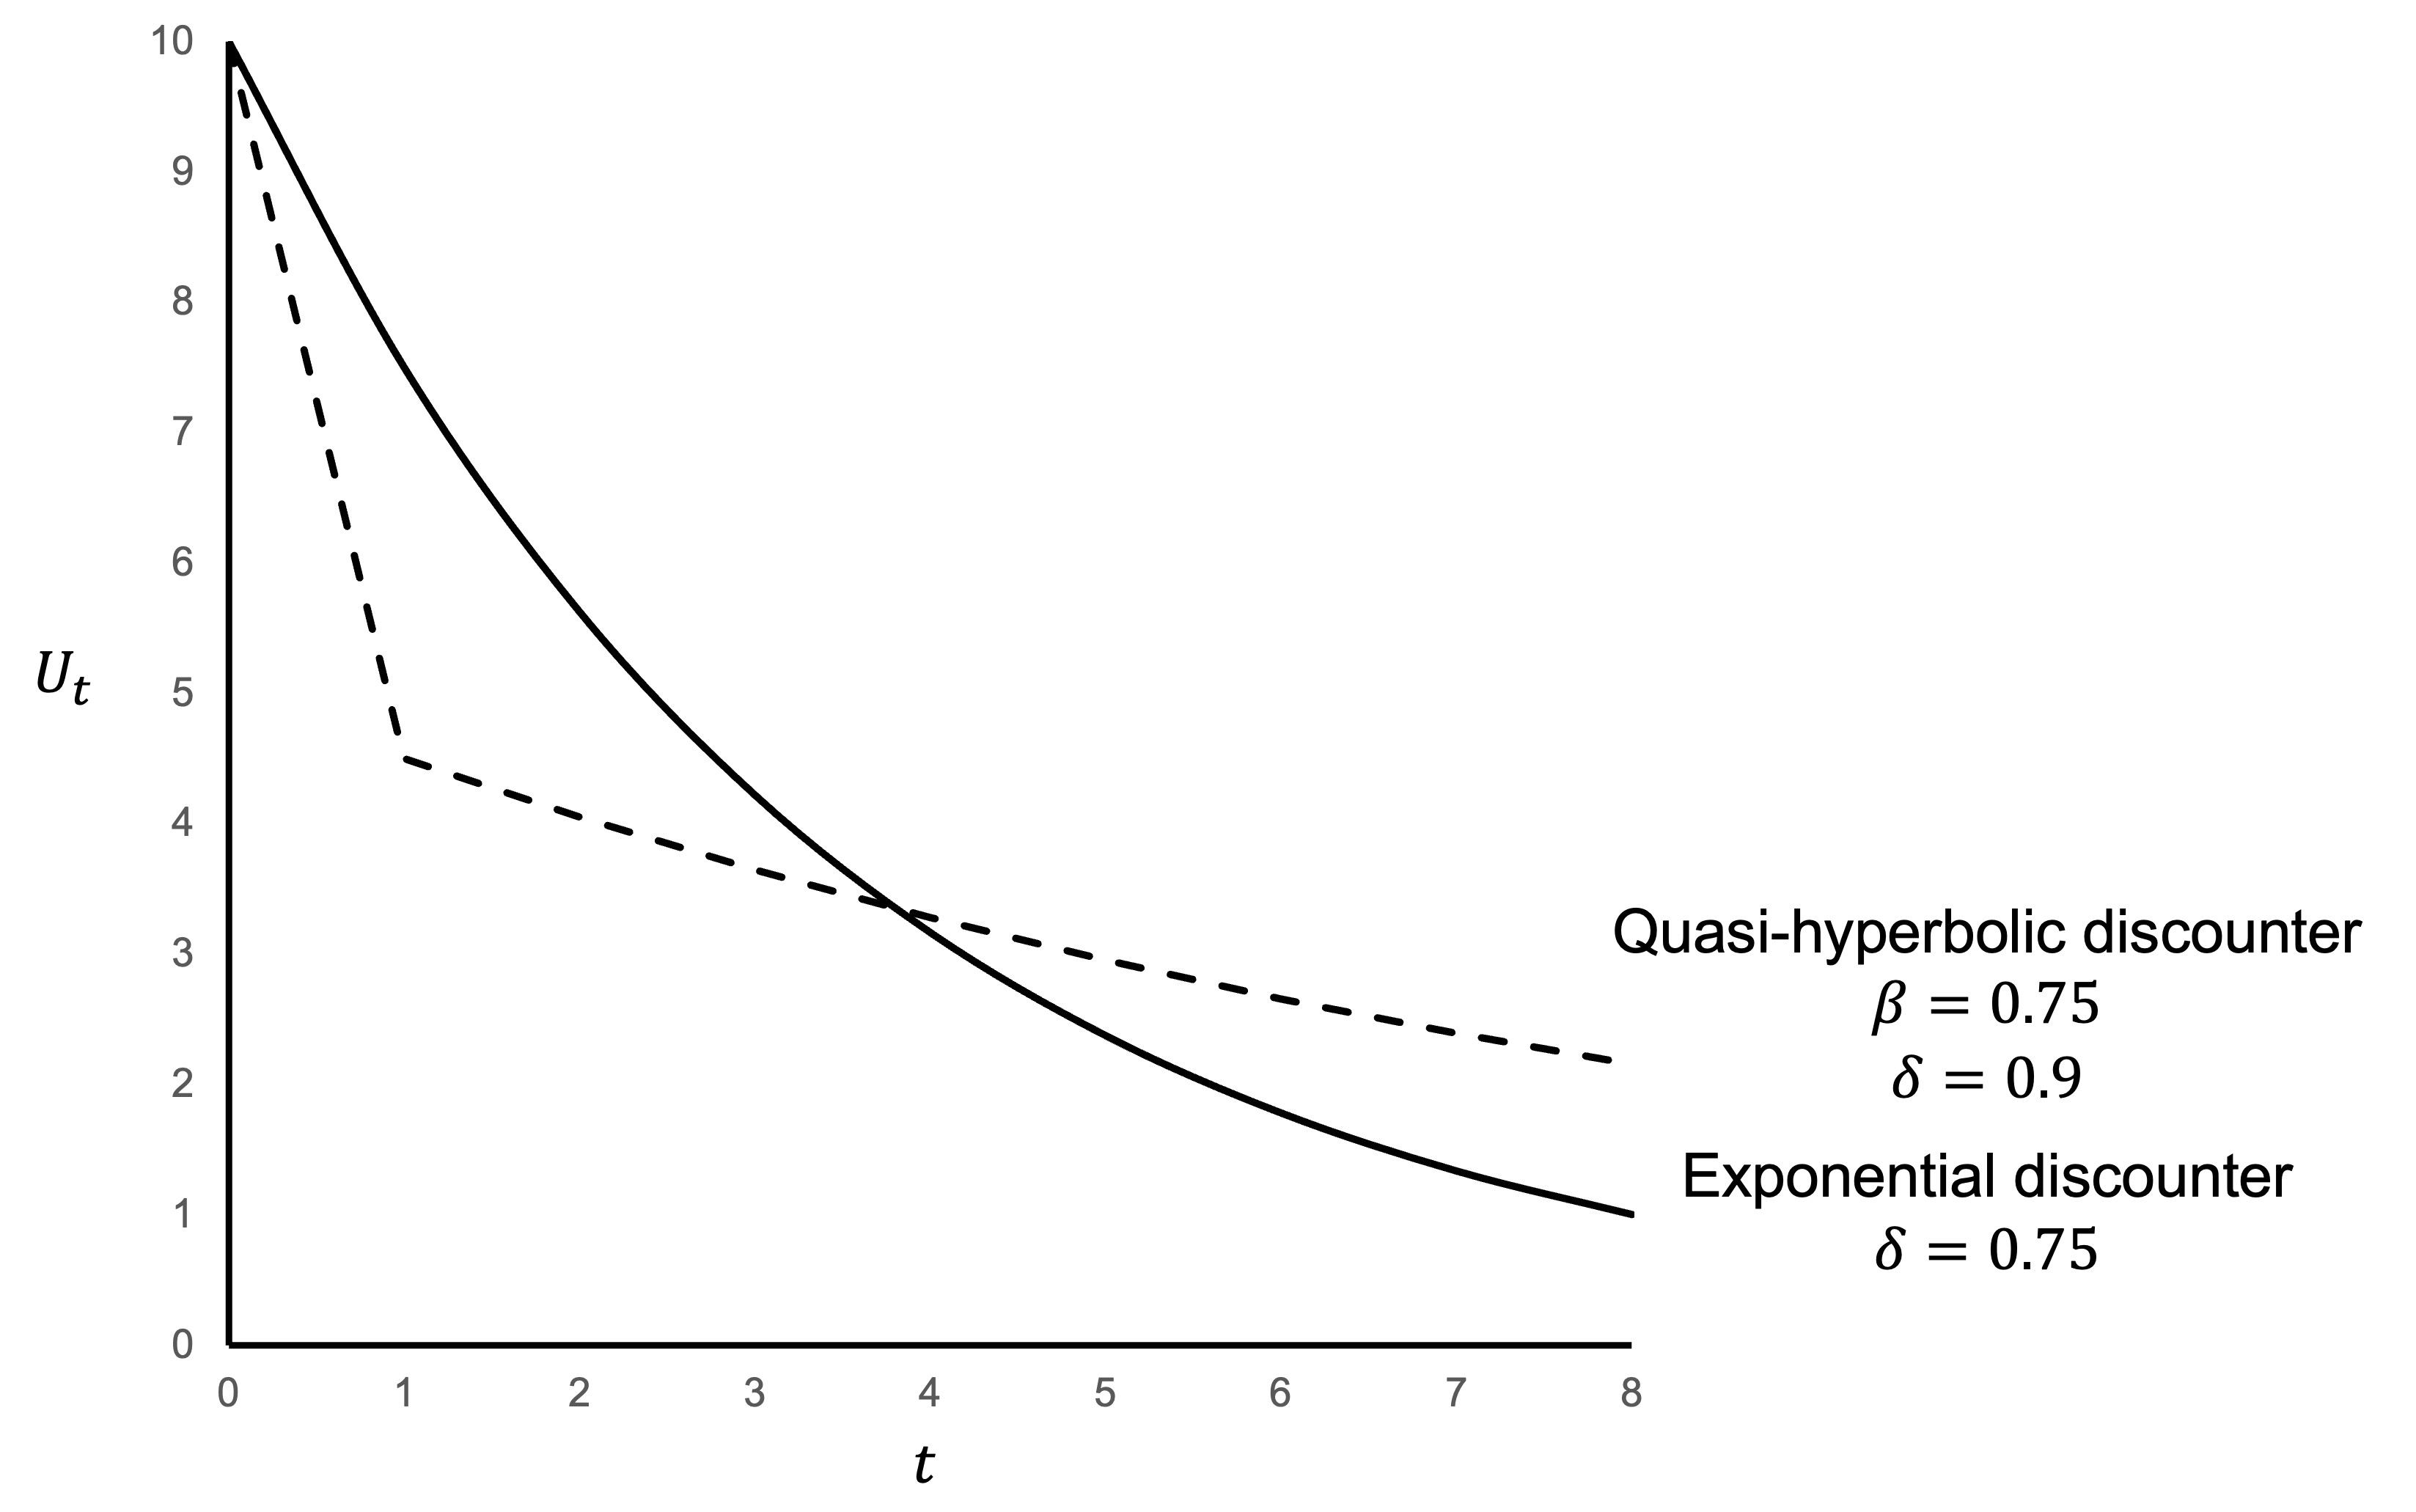
\includegraphics{intertemporal-choice/img/discount-curves-2.jpg}

\hypertarget{present-bias-examples}{%
\chapter{Present bias examples}\label{present-bias-examples}}

\hypertarget{example-1-3}{%
\section{Example 1}\label{example-1-3}}

Choice 1: Would you like \$100 today or \$110 next week?

Choice 2: Would you like \$100 next week or \$110 in two weeks?

\hypertarget{the-exponential-discounter}{%
\subsection{The exponential
discounter}\label{the-exponential-discounter}}

Suppose we have an exponential discounter with \(\delta=0.95\) and
utility each period of \(U(x_n)=x_n\).

Choice 1: Would this agent prefer \$100 today (\(t=0\)) or \$110 next
week (\(t=1\))?

We have already worked through this problem and determined that an
exponential discounter will prefer to receive \$110 next week.

Choice 2: Would this agent prefer \$100 next week (\(t=1\)) or \$110 in
two weeks (\(t=2\))?

Similarly, we previously determined that the exponential discounter will
prefer to receive \$110 in two weeks. The set of decisions across Choice
1 and Choice 2 are time consistent.

\hypertarget{the-present-biased-agent}{%
\subsection{The present-biased agent}\label{the-present-biased-agent}}

Suppose we have a present biased agent with \(\delta=0.95\),
\(\beta=0.95\) and utility each period of \(U(x_n)=x_n\).

Choice 1: Would this agent prefer \$100 today (\(t=0\)) or \$110 next
week (\(t=1\))?

\begin{align*}
U_0(0,\$100)&=u(\$100)\\
&-100
\end{align*}

\begin{align*}
U_0(1,\$110)&=\beta\delta u(\$110) \\
&=0.95*0.95*110 \\
&=99.275
\end{align*}

As \(U_0(0,\$100) > U_0(1,\$110)\), the present-biased agent will prefer
to receive \$100 this week.

Choice 2: Would this agent prefer \$100 next week (\(t=1\)) or \$110 in
two weeks (\(t=2\))?

\begin{align*}
U_0(1,\$100)&=\beta\delta u(\$100) \\
&=0.95*0.95*100 \\
&=90.25
\end{align*}

\begin{align*}
U_0(2,\$110)&=\beta\delta^2 u(\$110) \\
&=0.95*0.95^2*110 \\
&=94.31
\end{align*}

As \(U_0(1,\$100) < U_0(2,\$110)\), the present-biased agent will prefer
to receive \$110 in two weeks.

Putting those two choices together:

Choice 1: The present-biased agent will prefer \$100 now to \$110 in one
week. Their preference for benefits now (\(\beta\)) leads them to prefer
the immediate payoff.

Choice 2: The present-biased agent will prefer \$110 in two weeks to
\$100 in one week. They are willing to wait longer for a larger reward,
with both outcomes in the future and subject to the short-term discount
(\(\beta\)).

Consider what would happen if they selected the \$110 in two weeks in
Choice 2, but after one week were asked if they would like to reconsider
their choice. They are effectively being offered Choice 1. This would
then lead them to change their mind and take the immediate \$100.

This combination of decisions is time inconsistent. The agent's actions
are not consistent with their own initial plan.

\hypertarget{example-2-3}{%
\section{Example 2}\label{example-2-3}}

Suppose we have a present-biased agent with \(\beta=0.75\),
\(\delta=0.9\) and utility each period of \(u(x_n)=x_n\).

Would this agent prefer \$10 in five days (\(t=5\)) or \$20 in 10 days
(\(t=10\))?

\begin{align*}
U_0(5,\$10)&=\beta\delta^5u(\$10) \\
&=0.75\times 0.9^5\times 10 \\
&=4.429 \\
\\
U_0(10,\$20)&=\beta\delta^10 u(\$20) \\
&=0.75\times 0.9^{10}\times 20 \\
&=5.23
\end{align*}

This present-biased agent will prefer to receive \$20 in 10 days.

Five days pass and the agent is now asked if they would like to change
their mind.

\begin{align*}
U_5(5,\$10)&=u(\$10) \\
&=10
\\
U_5(10,\$20)&=\beta\delta^5 u(\$20) \\
&=0.75\times 0.9^5\times 20 \\
&=8.857
\end{align*}

We can see this change in preference in the following diagram. At
\(t=0\) (and through to \(t=4\)) the \$20 at \(t=10\) is preferred. At
\(t=5\) when the \$10 is no longer discounted by \(\beta\) it suddenly
becomes more attractive.

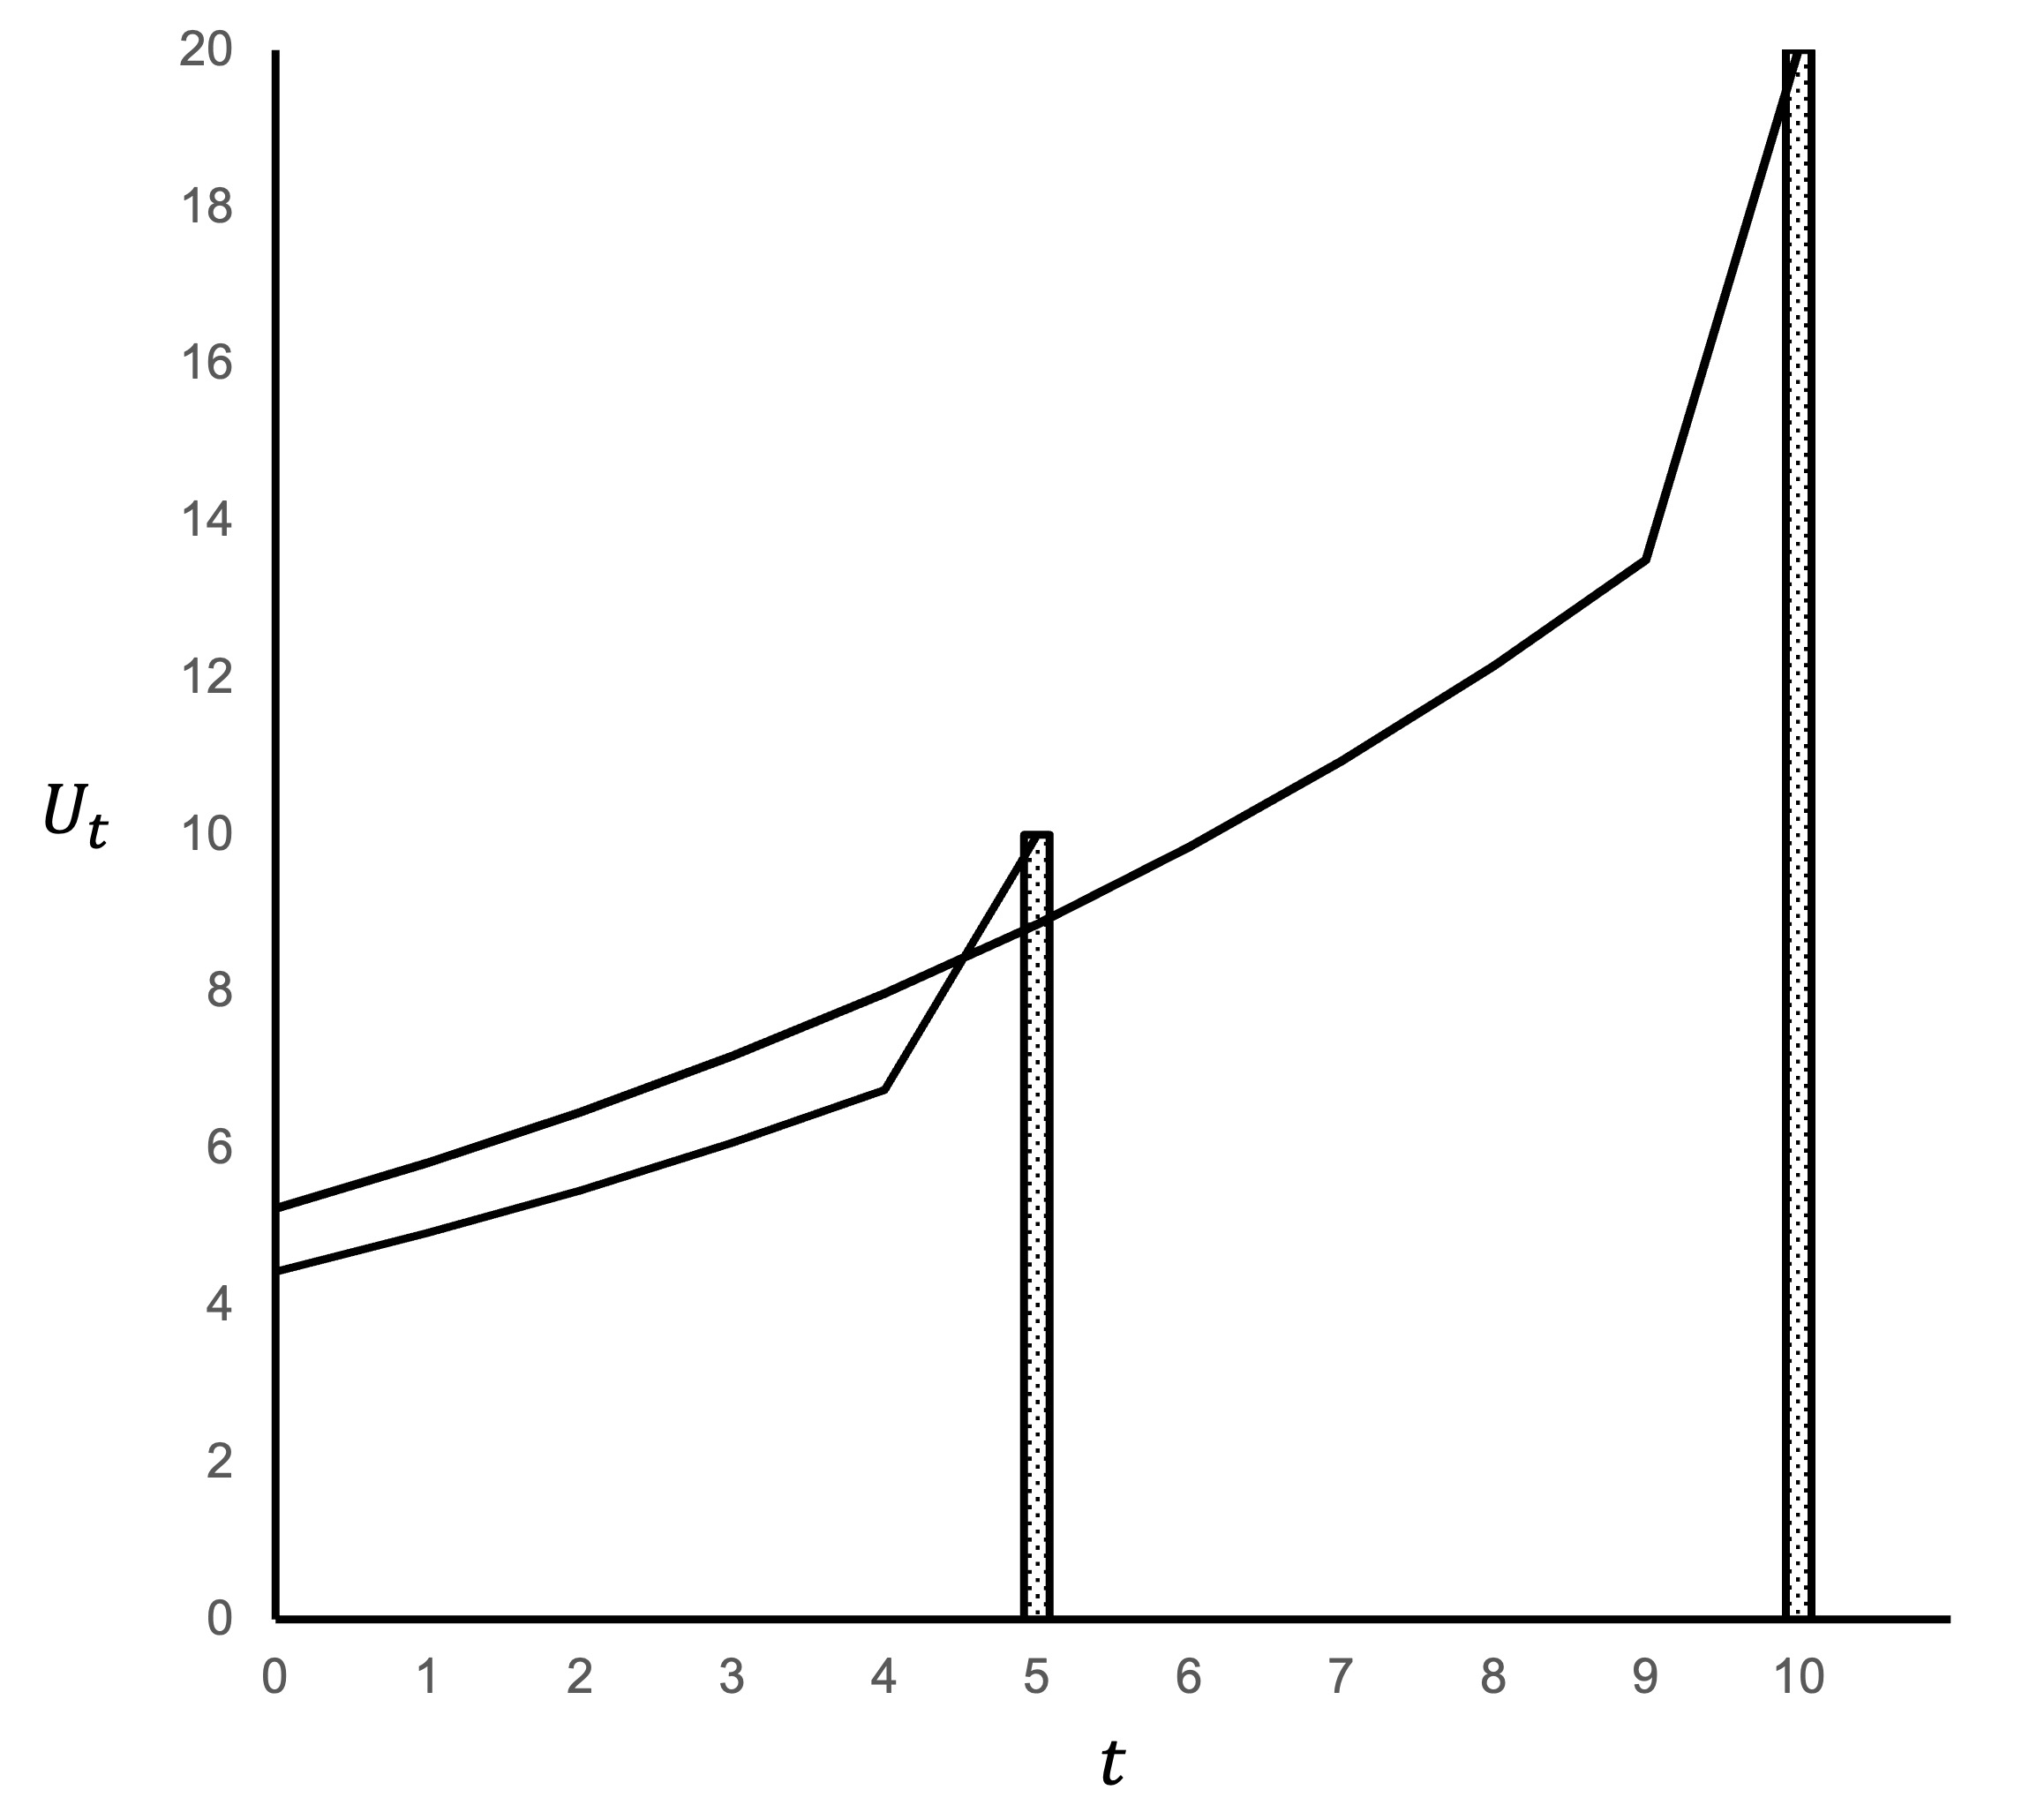
\includegraphics[width=0.75\textwidth,height=\textheight]{intertemporal-choice/img/present-bias-example-2.jpg}

\hypertarget{sophisticated-present-bias}{%
\chapter{Sophisticated present bias}\label{sophisticated-present-bias}}

In our analysis of present bias, I have made an implicit assumption that
the agent is unaware that their present-bias will lead them to make
inconsistent decisions over time. This present-biased agent decides that
they will wait for a larger, later pay-off despite the possibility that
they will change their mind when a smaller pay-off becomes immediately
available. The larger pay-off is never truly available to them.

For many of us, this does not match our experience. We know that we
often cave when faced with immediate temptation. And more than that,
because of our self-awareness we often plan around it. We hide the jar
of cookies or do not keep them in the house. We place our money in
savings account with no special features beyond an inability to access
the money.

To bring this idea into our analysis, I am going to distinguish between
two types of present-biased agents: naive and sophisticated
present-biased agents.

\hypertarget{nauxefve-and-sophisticated-present-biased-agents}{%
\section{Naïve and sophisticated present-biased
agents}\label{nauxefve-and-sophisticated-present-biased-agents}}

A naive present-biased agent discounts all future periods but
incorrectly believes that they do not have this problem in the future.

A sophisticated present-biased agent discounts all future periods and
correctly believes that they will also have this problem in the future.
They understand that if faced with the temptation to take benefits today
or delay costs, they will do so.

A sophisticated and naive person can make different decisions despite
having the same level of impatience, \(\delta\), and the same level of
present bias, \(\beta\).

The naive agent makes its plans by forward reasoning, starting from
today (\(t=0\)).

\begin{enumerate}
\def\labelenumi{\arabic{enumi}.}
\item
  First they decide their preferred option, believing they will stick to
  the plan once they move to next period.
\item
  When they move to next time period (\(t+1\)) they recompute their
  optimal plan, again believing they will stick to the plan once they
  move to next period.
\item
  They repeat this process as they move through time.
\end{enumerate}

The sophisticated agent makes its plans by backward reasoning, starting
from the final time period (\(t=T\)).

\begin{enumerate}
\def\labelenumi{\arabic{enumi}.}
\item
  For that final time period, they solve for the optimal action
\item
  Go back one time period (\(t=T-1\)) and solve for preferred action,
  accounting for the decision in (1)
\item
  Iterate
\end{enumerate}

\hypertarget{examples}{%
\section{Examples}\label{examples}}

\hypertarget{example-1-4}{%
\subsection{Example 1}\label{example-1-4}}

Suppose we have a naive and a sophisticated present-biased agent, each
with \(\delta=0.95\), \(\beta=0.95\) and utility each period of
\(U(x_n)=x_n\).

We offer them the following choice.

\begin{quote}
Would you like \$100 next week or \$110 in two weeks?
\end{quote}

We also tell them that we will give them the opportunity to reconsider
their decision next week.

The present-based agent that we examined in the earlier example was
naïve. They did not realise that they would change their mind if offered
that opportunity after a week. They would be surprised by that change.

When making their initial decision, the comparison they are making from
the perspective of today is simply between the discounted utilities from
the perspective of today:

\begin{align*}
U_0(1,\$100)&=90.25 \\
\\
U_0(2,\$110)&=94.32
\end{align*}

But this is an incorrect view as to their preferences next week. Next
week they will calculate utility as:

\begin{align*}
U_1(1,\$100)&=100 \\
\\
U_1(2,\$100)&=99.275
\end{align*}

Today they hold an incorrect belief as to what their preference will be
next week .

The sophisticated agent will first consider how they will look at the
choice next week:

\begin{align*}
U_1(1,\$1001)&=100 \\
\\
U_1(2,\$110)&=99.275
\end{align*}

The sophisticated agent sees that next week they will take the \$100.

As a result, today the sophisticated agent will choose \$100 in one
week. They see their future decision and know that \$110 in two weeks is
not available to them. They effectively accept their future present bias
now.

In this example, being naive or sophisticated does not change their
final decision. It only changes their beliefs about their final decision
before they reach it.

\hypertarget{example-2-4}{%
\subsection{Example 2}\label{example-2-4}}

Suppose we have a naive and a sophisticated present-biased agent, each
with \(\delta=1\), \(\beta=0.5\) and utility each period of
\(U(x_n)=x_n\). They are present-biased, but beyond that present-bias
demonstrate no impatience.

We offer them the following choice.

\begin{itemize}
\item
  \$6 today (\(t=0\))
\item
  \$10 in one week (\(t=1\))
\item
  \$16 in two weeks (\(t=2\))
\end{itemize}

They are also told that next week they will be offered an opportunity to
change their mind.

{[}Note: I am using \$ for many of these examples, but these could
equally be many other things: e.g.~three movies that each provide 6, 10
or 16 utility and you can only afford to attend one.{]}

First, we consider the naive agent. They calculate utility from the
perspective of today.

\begin{align*}
U_0(0,\$6)&=u(\$6) \\
&=6 \\
\\
U_0(1,\$10)&=\beta\delta u(\$10) \\
&=0.5*1*10 \\
&=5 \\
\\
U_0(2,\$16)&=\beta\delta^2 u(\$16) \\
&=0.5*1^2*16 \\
&=8
\end{align*}

The naive agent will choose the \$16 in two weeks.

But what then happens when the naive agent is given the chance to change
their mind after one week.

\begin{align*}
U_1(\$10 \text{ at }t=1)&=u(\$10) \\
&=10 \\
\\
U_1(\$16 \text{ at }t=2)&=\beta\delta u(\$16) \\
&=0.5*1*16 \\
&=8
\end{align*}

The naive agent will change their mind and take the \$10.

What of our sophisticated agent? They will make their decision today
based on their correct beliefs about their future preferences. To do
this, they solve by backward induction. First, what will their decision
be next week?

\begin{align*}
U_1(1,\$10)&=u(\$10) \\
&=10 \\
\\
U_1(2,\$16)&=\beta\delta u(\$16) \\
&=0.5*1*16 \\
&=8
\end{align*}

The sophisticated agent can see that they will choose to receive \$10
immediately when asked next week.

Knowing this is the case, the sophisticated agent now decides whether
they prefer the \$6 today or the \$10 next week.

\begin{align*}
U_0(0,\$6)&=u(\$6) \\
&=6 \\
\\
U_0(1,\$10)&=\beta\delta u(\$10) \\
&=0.5*1*10 \\
&=5
\end{align*}

They prefer the \$6 today.

The result is that the sophisticated agent will choose the \$6 today.
From today's perspective, they would prefer the \$16 in two weeks, but
as they know they will cave in to their present bias next week and take
the \$10, they make today's decision on that basis.

\hypertarget{example-3-2}{%
\subsection{Example 3}\label{example-3-2}}

A naive present-biased agent has failed to return their library books
and is fined at at \(t=0\). They can select one of the following payment
schemes:

\((0,-\$10)\), \((1,-\$15)\) or \((2,-\$25)\)

That is, they can pay \$10 today, \$15 at \(t=1\) or \$25 at \(t=2\).

They are free to change the scheme over time as they see fit.

The agent's utility is linear in money \(U(x_n)=x_n\), with discount
factors \(\delta=1\) and \(\beta=0.5\).

We start calculating utility from today:

\begin{align*}
U_0(0,-\$10)&=u(-\$10) \\
&=-10 \\
\\
U_0(1,-\$15)&=\beta\delta u(-\$15) \\
&=0.5*1*(-15) \\
&=-7.5 \\
\\
U_0(2,-\$25)&=\beta\delta^2 u(-\$25) \\
&=0.5*1^2*(-25) \\
&=-12.5
\end{align*}

The naive agent will choose to pay \$15 at \(t=1\).

Now we move to \(t=1\), when the naive agent reconsiders their decision:

\begin{align*}
U_1(1,-\$15)&=u(-\$15) \\
&=-15 \\
\\
U_1(2,-\$25)&=\beta\delta u(-\$25) \\
&=0.5*1*(-25) \\
&=-12.5
\end{align*}

The naive agent will choose to change their decision and further delay
their payment. They will now choose to pay \$25 at \(t=2\).

When they reach \(t=2\), they have no choice but to pay the \$25.

A sophisticated present-biased agent has failed to return their library
books and is fined at t =0. They can select one of the following payment
schemes:

\((0,-\$10)\), \((1,-\$15)\) or \((2,-\$25)\)

That is, they can pay \$10 today, \$15 at \(t=1\) or \$25 at \(t=2\).

They are free to change the scheme over time as they see fit.

The agent's utility is linear in money \(U(x_n)=x_n\), with discount
factors \(\delta=1\) and \(\beta=0.5\).

For the sophisticated agent, we start calculating utility from the final
period.

At \(t=2\), they have no choice but to pay the \$25.

What of \(t=1\)?

\begin{align*}
U_1(1,-\$15)&=u(-\$15) \\
&=-15 \\
\\
U_1(2,-\$25)&=\beta\delta u(-\$25) \\
&=0.5*1*(-25) \\
&=-12.5
\end{align*}

The sophisticated agent can see that if they make a choice at \(t=1\),
they will choose to pay \$25 at t = 2.

Now we iterate at t = 0. The sophisticated agent only compares \$10 at
\(t=0\) with \$25 at \(t=2\) because they know that at \(t=1\) they will
select \$25 at \(t=2\). They know that if they delay once they will
delay again and end up paying the largest fine. Hence they limit their
comparison to those outcomes that might occur:

\begin{align*}
U_0(0,-\$10)&=u(-\$10) \\
&=-10 \\
\\
U_0(2,-\$25)&=\beta\delta^2 u(-\$25) \\
&=0.5*1^2*(-25) \\
&=-12.5
\end{align*}

As \(U_0(0,-\$10)>U_0(2,-\$25)\), the sophisticated agent will choose to
pay \$10 at \(t=0\).

In our examples we have seen two contrasting outcomes for the
sophisticated agent.

In one example they took \$6 today (rather than \$10 in one week or \$16
in two) because they knew that they would take the \$10 in one week.
They took the lowest possible outcome.

In the latest example, they paid the lowest possible fine as they saw
they would further delay paying the fine in the future, leading it to
increase even more.

Suboptimality of sophisticated behaviour arises from two tensions:

\begin{enumerate}
\def\labelenumi{\arabic{enumi}.}
\item
  They understand that they will not be able to wait for the optimal
  time.
\item
  They are present-biased so prefer benefit today and costs delayed to
  the future.
\end{enumerate}

In combination, these imply a sophisticated agent will generally take
action earlier than the naive agent. They can ``prepoperate'', which is
doing something now when it would be better to wait.

\hypertarget{commitment}{%
\chapter{Commitment}\label{commitment}}

\hypertarget{definition}{%
\section{Definition}\label{definition}}

A commitment device is a mechanism which locks yourself into a course of
action that you might not otherwise choose but that produces the desired
result.

Commitment devices may work through the following channels:

\begin{itemize}
\item
  Artificially depressing the value of the bad course of action
\item
  Artificially increasing the value of the optimal course of action
\item
  Forcing the agent to maintain the optimal course of action.
\end{itemize}

\hypertarget{commitment-examples}{%
\section{Commitment examples}\label{commitment-examples}}

\hypertarget{forcing-the-optimal-course-of-action}{%
\subsection{Forcing the optimal course of
action}\label{forcing-the-optimal-course-of-action}}

Recall what the sophisticated present-biased agent with \(\beta=0.5\)
and \(\delta=1\) did when faced with a choice of (0, \$6; 1, \$10; 2,
\$16). First they realised that next week they would take the \$10
straight away.

\begin{align*}
U_1(1,\$10)&=u(\$10) \\
&=10 \\
\\
U_1(2,\$16)&=\beta\delta u(\$16) \\
&=0.5\times 1\times 16 \\
&=8
\end{align*}

Knowing this is the case, they then chose to take the \$6 today.

\begin{align*}
U_0(0,\$6)&=u(\$6) \\
&=6 \\
\\
U_0(1,\$10)&=\beta\delta u(\$10) \\
&=0.5\times 1\times 10 \\
&=5
\end{align*}

But when they compare all three, they would prefer the \$16 in two
weeks. It is only because they can foresee their future failing after
one week that they don't wait.

\begin{align*}
U_0(0,\$6)&=u(\$6) \\
&=6 \\
\\
U_0(1,\$10)&=\beta\delta u(\$10) \\
&=0.5\times 1\times 10 \\
&=5 \\
\\
U_0(2,\$16)&=\beta\delta^2 u(\$16) \\
&=0.5\times 1^2\times 16 \\
&=8
\end{align*}

But what if they could commit themselves today?

Suppose that not only could they select an option today, but they could
also choose to bind themselves to that decision such that they could not
change it in the future. The result of that: a sophisticated
present-biased agent would choose the \$16 in two weeks, and bind their
future self from changing their mind.

\[
U_0(0,\$6)=6
\]

\[
U_0(0,\$10)=5
\]

\[
U_0(0,\$16)=6
\]

\hypertarget{forcing-the-optimal-course-of-action-odysseus}{%
\subsection{Forcing the optimal course of action:
Odysseus}\label{forcing-the-optimal-course-of-action-odysseus}}

Another example of forcing the agent to maintain the optimal course of
action is the story of Odysseus.

Odysseus was required to sail past the sirens at \(t=1\). At that time
he can either jump off his ship to join the sirens (and die) or sail on
past and live.

As Odysseus is a sophisticated present-biased agent, he considers what
he is likely to do at that time. He realises that he will jump of the
ship for the immediate benefit of joining the sirens at the loss of the
longer-term benefit of living.

But from the perspective of Odysseus today, with both the benefits of
the siren and living in the future discounted, Odysseus would prefer to
live. As a result, he decides to commit himself to that course of action
by instructing his crew to tie him to the mast (plus leaving his ears
unplugged so that he also gets some benefits from the siren song).

\begin{figure}

{\centering 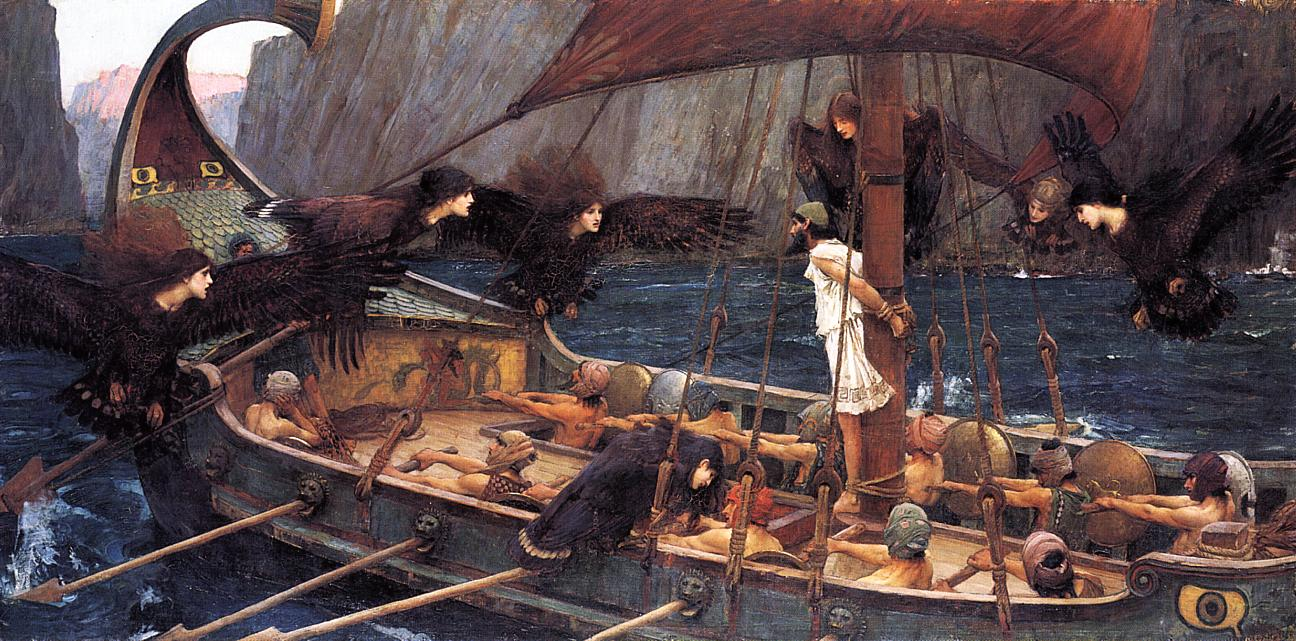
\includegraphics{intertemporal-choice/img/John_William_Waterhouse_-_Ulysses_and_the_Sirens_(1891).jpg}

}

\caption{\href{https://commons.wikimedia.org/wiki/File:John_William_Waterhouse_-_Ulysses_and_the_Sirens_(1891).jpg}{John
William Waterhouse, Ulysses and the Sirens (1891)}}

\end{figure}

\hypertarget{forcing-the-optimal-course-of-action-lay-by}{%
\subsection{Forcing the optimal course of action:
lay-by}\label{forcing-the-optimal-course-of-action-lay-by}}

Lay-by involves paying a deposit and administrative fee toward the
purchase of a product. You receive your purchase when you make payment
in full some time later.

Let us see how that could help a quasi-hyperbolic discounter with
discount factors \(\delta=1\) and \(\beta=1/2\).

Suppose you want a new jacket for work. You need to save for three
months to purchase the jacket. But each month you save you forgo
consumption that would boost your utility. Today you decide whether you
will save for the jacket or not.

You receive the following payoffs for each course of action:

\begin{longtable}[]{@{}lccc@{}}
\toprule()
& t=0 & t=1 & t=2 \\
\midrule()
\endhead
Save & 0 & 0 & 45 \\
Spend & 10 & 10 & 10 \\
\bottomrule()
\end{longtable}

First, consider what a naive quasi-hyperbolic discounter chooses.

At \(t=0\) the highest discounted utility is for Save. You plan to save
for the jacket.

\begin{align*}
U_0(\text{Save})&=0+\beta\delta \times 0+\beta\delta^2\times 45 \\
&=0.5\times 45 \\
&=22.5 \\
\\
U_0(\text{Spend})&=10+\beta\delta \times 10+\beta\delta^2\times 10 \\
&=10+0.5\times 10+0.5\times 10 \\
&=20
\end{align*}

One month now passes. You have saved for a month. You could now spend
both your savings from last month and this month, giving a short term
boost, or keep saving for your jacket.

\begin{longtable}[]{@{}lcc@{}}
\toprule()
& t=1 & t=2 \\
\midrule()
\endhead
Save & 0 & 45 \\
Start spending at \(t=1\) & 20 & 10 \\
\bottomrule()
\end{longtable}

At \(t=1\) spending now has the highest discounted utility. After saving
for the first period, you spend despite initially wanting to save.

\begin{align*}
U_1(\text{Save})&=0+\beta\delta\times 45 \\
&=0.5\times 45 \\
&=22.5 \\
\\
U_1(\text{Start spending at t=1})&=20+\beta\delta \times 10 \\
&=20+0.5\times 10 \\
&=25
\end{align*}

Now let's consider this problem from the point of view of a
sophisticated present-biased agent. They see their full choice set as:

\begin{longtable}[]{@{}lccc@{}}
\toprule()
& t=0 & t=1 & t=2 \\
\midrule()
\endhead
Save & 0 & 0 & 45 \\
Start spending at t=1 & 0 & 20 & 10 \\
Spend & 10 & 10 & 10 \\
\bottomrule()
\end{longtable}

You work backward through time. At \(t=2\), you will buy the jacket.

The utility of each option at \(t=1\) is as follows:

\begin{align*}
U_1(\text{Save})&=0+\beta\delta\times 45 \\
&=0.5\times 45 \\
&=22.5 \\
\\
U_1(\text{Start spending at }t=1)&=20+\beta\delta \times 10 \\
&=20+0.5\times 10 \\
&=25
\end{align*}

If the agent had spent at \(t=0\), you have no choice but to spend at
\(t=1\).

The sophisticated quasi-hyperbolic discounter now knows that saving for
the jacket is not available to them as they will spend at \(t=1\)
regardless of their initial actions. As a result, at \(t=0\) they choose
between the two feasible options:

\begin{align*}
U_0(\text{Start spending at }t=1)&=0+\beta\delta \times 20+\beta\delta^2\times 10 \\
&=0.5\times 20+0.5\times 10 \\
&=15 \\
\\
U_0(\text{Save})&=10+\beta\delta \times 10+\beta\delta^2\times 10 \\
&=10+0.5\times 10+0.5\times 10 \\
&=20
\end{align*}

They start to spend at \(t=0\). Contrast this with the naïve agent who
chooses Save at \(t=0\). The sophisticated agent would also prefer Save
at \(t=0\), but knows that Save is not available to them as they will
spend at \(t=1\).

Now consider what the sophisticated agent may do in the presence of
lay-by.

For payment of an administrative fee equivalent to 1 unit of utility and
an initial deposit (the agent's savings in \(t=0\)), you reserve the
jacket, preventing you from spending that money in period 2. The new set
of options is:

\begin{longtable}[]{@{}lccc@{}}
\toprule()
& t=0 & t=1 & t=2 \\
\midrule()
\endhead
Save & 0 & 0 & 45 \\
Start spending at t=1 & 0 & 20 & 10 \\
Spend & 10 & 10 & 10 \\
Lay-by & -1 & 0 & 45 \\
\bottomrule()
\end{longtable}

The lay-by option is strictly worse than Save. But what happens if
lay-by is available to the sophisticated present-biased agent?

Again, working backward, at \(t=2\), the agent buys the jacket.

At \(t=1\), by the same logic we looked at previously, they spend if
they are able to do so. That eliminates Save from their choice set. At
\(t=0\), they now compare the feasible options:

\begin{align*}
U_0(\text{Start spending at }t=1)&=0+\beta\delta \times 20+\beta\delta^2\times 10 \\
&=0.5\times 20+0.5\times 10 \\
&=15 \\
\\
U_0(\text{Spend})&=10+\beta\delta \times 10+\beta\delta^2\times 10 \\
&=10+0.5\times 10+0.5\times 10 \\
&=20 \\
\\
U_0(\text{Lay-by})&=-1+\beta\delta \times 0+\beta\delta^2\times 45 \\
&=-1+0.5\times 0+0.5\times 45 \\
&=21.5
\end{align*}

Lay-by is the preferred option at \(t=0\). As it binds the agent in the
future, they are able to stick to this plan.

Note that Lay-by is strictly worse than Save as the agent must pay the
administrative fee. But the sophisticated quasi-hyperbolic discounter
chooses it as the only feasible way to get their jacket. Without Lay-by
they know they will Start spending at \(t=1\) and end up with lower
utility from the perspective of their \(t=0\) self.

\hypertarget{depressing-the-value-of-the-bad-course-of-action}{%
\subsection{Depressing the value of the bad course of
action}\label{depressing-the-value-of-the-bad-course-of-action}}

\href{https://www.stickk.com}{stickK} is a online platform that enables
people to commit to future courses of action. stickK works as follows:

\begin{enumerate}
\def\labelenumi{\arabic{enumi}.}
\item
  You state a time-based goal, such as not smoking during the next
  month, losing 5kg over the next 90 days, or writing the next chapter
  of your PhD thesis by Christmas.
\item
  You commit a stake that will be paid to a charity (or an anti-charity)
  if you fail to meet your goal.
\item
  At the stated time you report (or a referee appointed by you reports)
  whether you have met your goal.
\item
  If you fail to report or report that you failed to meet your goal,
  your credit card is debited by the staked amount.
\end{enumerate}


\includegraphics{intertemporal-choice/img/stickk.jpg}

The following is an illustration of how it works mathematically.

A sophisticated present-biased agent with \(\delta=1\) and \(\beta=1/2\)
enjoys smoking. Smoking gives utility of 5. However, the agent also
likes being healthy. Higher health gives utility of 8.

At \(t=0\) the agent is deciding whether to smoke over the next month
(\(t=1\)). If the agent doesn't smoke, it will have better health at
\(t=2\).

The sophisticated agent works backward through time. At \(t=1\) its
payoffs are:

\begin{align*}
U_1(\text{smoking})&=5 \\
\\
U_1(\text{healthy})&=\beta\delta\times 8 \\
&=4
\end{align*}

The agent decides to smoke.

As a result, at \(t=0\), knowing that it will cave at \(t=1\), the agent
doesn't bother committing to not smoking, even though from the
perspective of \(t=0\) refraining from smoking is the better option:

\begin{align*}
U_0(\text{smoking})&=\beta\delta\times 5 \\
&=2.5
\\
U_0(\text{healthy})&=\beta\delta^2\times 8 \\
&=4
\end{align*}

But now suppose the agent learns about stickK. The agent now has the
option of staking a sum at \(t=0\) to prevent it from smoking. The agent
decides to stake an amount equivalent to utility 5 that would be
incurred at \(t=2\).

Working backward through time, the agent knows that at \(t=1\) if it has
not staked any money with stickK, it will smoke. But what if it has?

\begin{align*}
U_1(\text{stickK+smoking})&=5-\beta\delta\times 5 \\
&=2.5
\\
U_1(\text{stickK+healthy})&=\beta\delta\times 8 \\
&=4
\end{align*}

The agent would refrain from smoking at \(t=1\) due to the penalty it
would have to pay.

This means the agent's options at \(t=0\) are effectively:

\begin{align*}
U_0(\text{smoking})&=\beta\delta\times 5 \\
&=2.5
\\
U_0(\text{stickK+healthy})&=\beta\delta^2\times 8 \\
&=4
\end{align*}

The agent chooses to commit using stickK.

For a problem of this form the agent could always successfully use
stickK to commit to any action. The agent just needs to make the stake
high enough.

\hypertarget{increasing-the-value-of-the-optimal-action-temptation-bundling}{%
\subsection{Increasing the value of the optimal action: temptation
bundling}\label{increasing-the-value-of-the-optimal-action-temptation-bundling}}

``Temptation bundling'' involves increasing the value of the optimal
course of action by adding a temptation to that course.

Consider the following example.

Beth has the choice between the following options:

\begin{itemize}
\item
  Exercising at \(t=0\) (utility = 0) which leads her to being healthy
  and happy at time 1 (utility = 12)
\item
  Watching television at time 0 (utility = 6) and being unhealthy and
  unhappy at time 1 (utility = 0)
\end{itemize}

Beth discounts the future quasi-hyperbolically. Beth's \(\beta=1/2\) and
her \(\delta=2/3\). Does Beth exercise?

We solve as follows:

\begin{align*}
U_0(\text{exercise})&=u(x_0)+\beta\delta u(x_1) \\
&=0+\frac{1}{2}\times {2}{3}\times 12 \\
&=4
\\
U_0(\text{television})&=u(x_0)+\beta\delta u(x_1) \\
&=6+\frac{1}{2}\times {2}{3}\times 0 \\
&=6
\end{align*}

Beth chooses to watch television.

But what if Beth loved massages and remembers she has a massage voucher
she has been saving? What if she decides that if she exercises today,
she will go for a massage straight after? Let us assume that the utility
of a massage is 3.

We solve as follows:

\begin{align*}
U_0(\text{exercise+massage})&=u(x_0)+\beta\delta u(x_1) \\
&=3+\frac{1}{2}\times {2}{3}\times 12 \\
&=7
\\
U_0(\text{television})&=u(x_0)+\beta\delta u(x_1) \\
&=6+\frac{1}{2}\times {2}{3}\times 0 \\
&=6
\end{align*}

Beth now chooses to exercise.

This example is not strictly a commitment device as Beth could cheat.
Beth could watch television and get the massage. But people are often
good at creating ``mental accounts'' by which they make certain money or
activities out-of-bounds unless certain conditions are met.

\hypertarget{preference-over-profiles}{%
\chapter{Preference over profiles}\label{preference-over-profiles}}

Recall the assumption of utility independence:

\begin{quote}
All that matters is maximizing the sum of discounted utilities. Decision
makers are assumed to have no preference for the distribution of
utilities.
\end{quote}

However, there is evidence that people care about the shape of the
utility stream over time. People don't care solely about maximizing
discounted utility. This includes evidence for delayed gratification,
spread and variation.

This is known as having a ``preference over profiles''.

If we have preferences over profiles, the assumption of utility
independence no longer holds.

\hypertarget{delayed-gratification}{%
\section{Delayed gratification}\label{delayed-gratification}}

Consider the following example:

\begin{quote}
It is a sunny weekend. You can either study today and go to the beach
tomorrow, or you can go to the beach today and study tomorrow.

Studying gives you a utility of 10. Going to the beach gives you a
utility of 20.
\end{quote}

What would an exponential discounter with \(\delta=0.8\) do?

What would a present-biased agent with \(\beta=0.5\) and \(\delta=0.8\)
do?

It is easy to determine that both agents would go to the beach today and
study tomorrow. They will always schedule pleasant tasks before
unpleasant tasks.

Does this match people's observed behaviour?

There is considerable evidence that people will schedule unpleasant
experiences first and pleasant ones later. This might be thought of as a
preference for an increasing utility profile.

How could this be possible for someone who discounts the future?

One way is to ease the requirement that \(\delta\) be less than one.
This provides a solution to the weekend problem, but also leads to the
potential of endlessly postponing pleasant experiences.

Easing this requirement also clashes with other evidence that people
often postpone unpleasant tasks and that people have a \(\delta\) much
less than one for many decisions.

\hypertarget{spread-of-utility}{%
\section{Spread of utility}\label{spread-of-utility}}

There is some evidence that we have a preference for spread of utility.

For example, if we have a box of chocolate, we often distribute eating
them over time (although at others we eat than all in one sitting).

\hypertarget{variation}{%
\section{Variation}\label{variation}}

We also have preference for variation.

\begin{quote}
You favourite meal is lasagna. Your second favourite meal is spaghetti
bolognaise. Your third favourite is fish and chips. You are offered the
following two options:

\begin{enumerate}
\def\labelenumi{\arabic{enumi}.}
\tightlist
\item
  Lasagna every night for the next week.
\item
  Alternating meals of lasagna, spaghetti and fish and chips.
\end{enumerate}
\end{quote}

We don't choose to have the same good or service over and over.

\hypertarget{intertemporal-choice-applications}{%
\chapter{Intertemporal choice
applications}\label{intertemporal-choice-applications}}

\hypertarget{savings}{%
\section{Savings}\label{savings}}

In the 1960s, the domestic savings rate in the Philippines was over 20\%
of GDP (one of the highest in Asia). By 2006, the savings rate ranges
between 12 and 15 percent, far below the level of savings for most East
Asian countries.

Ashraf et al. (2006) offered a commitment savings product called SEED
(Save, Earn, Enjoy Deposits) to randomly chosen clients of a Philippine
bank. SEED restricted access to savings for one year.

Other than providing a possible commitment savings device, no further
benefit accrued to individuals with this account.

\begin{itemize}
\tightlist
\item
  28.4\% take-up rate of the two commitment protocols studies (either
  goal or time-based goal).
\item
  Average savings balance increased by 42\% after six months and by 82\%
  after one year.
\end{itemize}

\hypertarget{smoking}{%
\section{Smoking}\label{smoking}}

Giné et al. (2010) tested a voluntary commitment product for smoking
cessation.

Smokers were offered a product (CARES) that comprised a savings account
in which they deposit funds. After six months they take urine tests for
nicotine and cotinine.

If they pass, the money is returned. Otherwise, it is forfeited.

The result was that 11\% of smokers offered CARES took it up. Smokers
offered CARES were 3 percentage points more likely to pass the 6-month
test than the control group

The effect persisted in a surprise tests at 12 months.

\hypertarget{gym-attendance}{%
\section{Gym attendance}\label{gym-attendance}}

Kirgios et al. (2020) found that:

\begin{itemize}
\item
  Teaching gym-goers how to temptation bundle with a free audiobook
  boosts gym visits.
\item
  People who are given audiobooks by gyms can infer they should
  temptation bundle.
\item
  Simply receiving a free audiobook with no explicit instruction boosts
  exercise.
\item
  Teaching temptation bundling modestly outperforms simply giving
  gym-goers free audiobooks.
\end{itemize}

\hypertarget{organ-donation}{%
\section{Organ donation}\label{organ-donation}}

In European countries there are registers of people who will donate
their organs in case of death. There is a considerable gap in the
percentage of registered organ donors. Why?

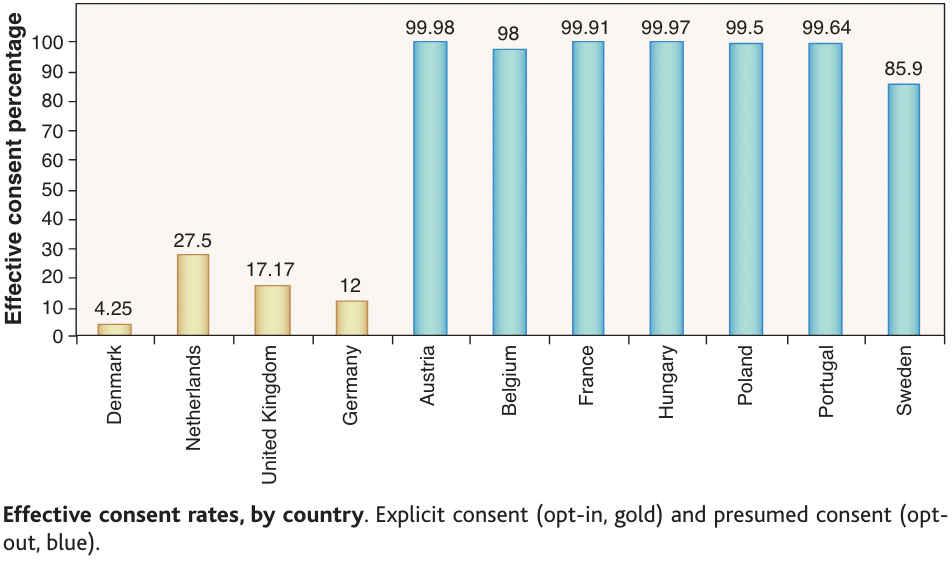
\includegraphics{intertemporal-choice/img/Johnson_and_Goldstein_2003_Figure.png}
Figure from E. J. Johnson and Goldstein (2003).

Yellow countries have an opt-in policy. People are required to register
as an organ donor.

Green countries have an opt-out policy known as presumed consent. They
are presumed to consent unless they opt-out (often through submission of
a form).

This is a classic example of a default effect. Defaults are sticky. The
stickiness of defaults is typically assumed to come from loss aversion
or present-bias.

\begin{itemize}
\item
  There is an immediate cost of changing from the default (time, effort,
  money). That cost is not discounted.
\item
  The future benefit of their action is discounted.
\item
  Agents put off a switch even though cost is low since they believe
  they will switch later.
\item
  Consequently, people do not exert their right to choose once they are
  allocated some options.
\end{itemize}

It is also possible to make an argument that the stickiness of the
defaults is due to a rational cost-benefit calculation, rather than due
to loss aversion of present bias.

\begin{itemize}
\item
  The cost of opting out is real.
\item
  People may not have a strong preference about whether they are an
  organ donor
\item
  Registration does not mean that your organs will be donated. Other
  factors such as family preference affect donation. As a result,
  registration might be seen as having little effect on the outcome you
  care about (actual organ donation). E. J. Johnson and Goldstein (2003)
  argue that there is a positive relationship between an opt-out policy
  and organ donations, but it is much weaker than the registration
  numbers would suggest and based on a simple regression that likely
  does not capture all relevant variables.
\item
  Further, the absence of any active consent in situations of presumed
  consent means that the family cannot take their presence on the organ
  donation register as an indication of the deceased's wishes.
\end{itemize}

Put together, the failure to opt-out may reflect a simple cost-benefit
analysis.

There are alternatives to presumed

One alternative is the use of defaults in a more transparent way where
opting out is easy. For example, when obtaining your driver's licence
there could be a section stating ``Please tick this box if you do not
wish to be registered as an organ donor''. This measure would likely
increase registration over the alternative of asking people to tick the
box if they wish to be an organ donor.

Another alternative is ``active choice'', where citizens are required to
indicate whether or not they wish to be registered. This could also be
built into a form such as a driver's licence application.

\hypertarget{save-more-tomorrow}{%
\section{Save More Tomorrow}\label{save-more-tomorrow}}

The Save More Tomorrow program (Richard~H. Thaler and Benartzi (2004))
combines principles relating to both prospect theory and time preference
to increase retirement savings.

Under Save More Tomorrow, customers are asked to commit in advance to
allocating a fraction of their future salary increases toward their
retirement savings accounts.

Save More Tomorrow is designed to reduce loss aversion as a factor in
deciding contribution amounts. A commitment of a proportion of pay rises
means that the contribution can increase over time, but pay never
decreases.

The program capitalises on participants' propensity to stick with the
status quo, as people are unlikely to unwind their future commitments
despite being able to opt out at any time.

That ability opt-out also reduces regret/disappointment aversion.

The first tests of the Save More Tomorrow program by Richard~H. Thaler
and Benartzi (2004) resulted in 78 per cent of those offered the plan
joining, 80\% of those remaining in the plan through the fourth pay
rise, and average savings rates increasing from 3.5\% to 13.6\% over 40
months. This compares to much lower savings rates by those who declined
advice, accepted a recommended savings rate or took advice but declined
to enrol in Save More Tomorrow.

\begin{figure}

{\centering 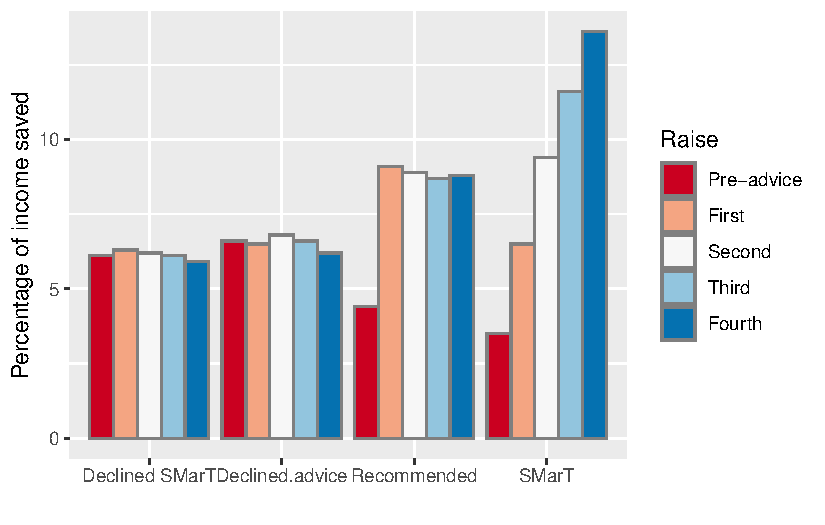
\includegraphics{intertemporal-choice/intertemporal-choice-applications_files/figure-pdf/fig-smart-1.pdf}

}

\caption{\label{fig-smart}Savings rates for SMarT}

\end{figure}

Note the savings rate is higher than the default rate in Australia.
Could the default in Australia create a low anchor for some people?

\hypertarget{intertemporal-choice-exercises}{%
\chapter{Intertemporal choice
exercises}\label{intertemporal-choice-exercises}}

\hypertarget{exercise-or-television}{%
\section{Exercise or television?}\label{exercise-or-television}}

Olga and Paul can choose one of the following options:

\begin{itemize}
\item
  Exercising at \(t=0\) (utility = 0) and being healthy at \(t=1\)
  (utility = 30).
\item
  Watching television at \(t=0\) (utility = 15) and being unhealthy at
  \(t=1\) (utility = 0).
\end{itemize}

a) Olga discounts the future exponentially with \(\delta=2/3\). At
\(t=0\), what is Olga's utility of exercising and watching television?
What does Olga do?

\begin{tcolorbox}[enhanced jigsaw, title=\textcolor{quarto-callout-tip-color}{\faLightbulb}\hspace{0.5em}{Answer}, toprule=.15mm, colback=white, breakable, titlerule=0mm, colframe=quarto-callout-tip-color-frame, coltitle=black, opacityback=0, rightrule=.15mm, colbacktitle=quarto-callout-tip-color!10!white, bottomtitle=1mm, opacitybacktitle=0.6, arc=.35mm, bottomrule=.15mm, toptitle=1mm, leftrule=.75mm, left=2mm]

\begin{align*}
U_0(exercise)&=u(x_0)+\delta u(x_1) \\
&=0+\frac{2}{3}\times 30 \\
&=20 \\
\\
U_0(television)&=u(x_0)+\delta u(x_1) \\
&=15+\frac{2}{3}\times 0 \\
&=15
\end{align*}

Olga gets higher discounted utility from exercising, so chooses to
exercise.

\end{tcolorbox}

b) Paul discounts the future quasi-hyperbolically with \(\beta=3/4\) and
\(\delta=2/3\). At \(t=0\), what is Paul's utility of exercising and
watching television? What does Paul do?

\begin{tcolorbox}[enhanced jigsaw, title=\textcolor{quarto-callout-tip-color}{\faLightbulb}\hspace{0.5em}{Answer}, toprule=.15mm, colback=white, breakable, titlerule=0mm, colframe=quarto-callout-tip-color-frame, coltitle=black, opacityback=0, rightrule=.15mm, colbacktitle=quarto-callout-tip-color!10!white, bottomtitle=1mm, opacitybacktitle=0.6, arc=.35mm, bottomrule=.15mm, toptitle=1mm, leftrule=.75mm, left=2mm]

\begin{align*}
U_0(exercise)&=u(x_0)+\beta\delta u(x_1) \\
&=0+\frac{3}{4}\times \frac{2}{3}\times 30 \\
&=15 \\
\\
U_0(television)&=u(x_0)+\beta\delta u(x_1) \\
&=6+\frac{3}{4}\times \frac{2}{3}\times 0 \\
&=15
\end{align*}

Paul is indifferent between the two options, so could choose either.

\end{tcolorbox}

\hypertarget{today-or-tomorrow}{%
\section{Today or tomorrow?}\label{today-or-tomorrow}}

Terry and Andy are given the choice between the following three options:

\begin{itemize}
\item
  A (utility of 3 at \(t=0\))
\item
  B (utility of 4 at \(t=1\))
\item
  C (utility of 5 at \(t=2\)).
\end{itemize}

a) Suppose that Terry discounts the future exponentially with
\(0<\delta<1\). He is indifferent between A and B at \(t=0\). What does
this tell you about Terry's \(\delta\)?

\begin{tcolorbox}[enhanced jigsaw, title=\textcolor{quarto-callout-tip-color}{\faLightbulb}\hspace{0.5em}{Answer}, toprule=.15mm, colback=white, breakable, titlerule=0mm, colframe=quarto-callout-tip-color-frame, coltitle=black, opacityback=0, rightrule=.15mm, colbacktitle=quarto-callout-tip-color!10!white, bottomtitle=1mm, opacitybacktitle=0.6, arc=.35mm, bottomrule=.15mm, toptitle=1mm, leftrule=.75mm, left=2mm]

The utility of A and B must be equal.

\begin{align*}
U_0(A)&=U_0(B) \\[6pt]
3&=\delta 4 \\[6pt]
\delta&=\frac{3}{4}
\end{align*}

\end{tcolorbox}

b) Andy discounts the future quasi-hyperbolically with \(0<\beta<1\) and
\(0<\delta<1\). At \(t=0\), Andy is indifferent between A and B. What
does this tell you about Andy's \(\beta\) and \(\delta\)?

\begin{tcolorbox}[enhanced jigsaw, title=\textcolor{quarto-callout-tip-color}{\faLightbulb}\hspace{0.5em}{Answer}, toprule=.15mm, colback=white, breakable, titlerule=0mm, colframe=quarto-callout-tip-color-frame, coltitle=black, opacityback=0, rightrule=.15mm, colbacktitle=quarto-callout-tip-color!10!white, bottomtitle=1mm, opacitybacktitle=0.6, arc=.35mm, bottomrule=.15mm, toptitle=1mm, leftrule=.75mm, left=2mm]

The utility of A and B must be equal.

\begin{align*}
U_0(A)&=U_0(B) \\[6pt]
3&=\beta\delta 4 \\[6pt]
\beta\delta&=\frac{3}{4}
\end{align*}

We cannot determine anything else about the two as the discounting
between \(t=0\) and \(t=1\) is a function of both the short-term and
exponential discount factor.

\end{tcolorbox}

c) At \(t=0\), Andy is indifferent between B and C. What does this tell
you about Andy's \(\beta\) and \(\delta\)?

\begin{tcolorbox}[enhanced jigsaw, title=\textcolor{quarto-callout-tip-color}{\faLightbulb}\hspace{0.5em}{Answer}, toprule=.15mm, colback=white, breakable, titlerule=0mm, colframe=quarto-callout-tip-color-frame, coltitle=black, opacityback=0, rightrule=.15mm, colbacktitle=quarto-callout-tip-color!10!white, bottomtitle=1mm, opacitybacktitle=0.6, arc=.35mm, bottomrule=.15mm, toptitle=1mm, leftrule=.75mm, left=2mm]

The utility of B and C must be equal.

\begin{align*}
U_0(B)&=U_0(C) \\[6pt]
\beta\delta 4&=\beta\delta^2 5 \\[6pt]
4&=\delta 5 \\
\delta&=\frac{4}{5}
\end{align*}

\end{tcolorbox}

d) Combining the results of (b) and (c), compute Andy's \(\beta\) and
\(\delta\)?

\begin{tcolorbox}[enhanced jigsaw, title=\textcolor{quarto-callout-tip-color}{\faLightbulb}\hspace{0.5em}{Answer}, toprule=.15mm, colback=white, breakable, titlerule=0mm, colframe=quarto-callout-tip-color-frame, coltitle=black, opacityback=0, rightrule=.15mm, colbacktitle=quarto-callout-tip-color!10!white, bottomtitle=1mm, opacitybacktitle=0.6, arc=.35mm, bottomrule=.15mm, toptitle=1mm, leftrule=.75mm, left=2mm]

We have already computed:

\begin{enumerate}
\def\labelenumi{(\arabic{enumi})}
\tightlist
\item
  \(\delta=\frac{4}{5}\).
\end{enumerate}

We also know:

\begin{enumerate}
\def\labelenumi{(\arabic{enumi})}
\setcounter{enumi}{1}
\tightlist
\item
  \(\beta\delta=\frac{3}{4}\)
\end{enumerate}

Accordingly, substituting (1) into (2):

\begin{align*}
\beta\frac{4}{5}=\frac{3}{4} \\
\beta=\frac{15}{16}
\end{align*}

\end{tcolorbox}

\hypertarget{sec-Q3}{%
\section{Today or tonight?}\label{sec-Q3}}

Kate and Jack have utility function \(u(x)=x\) and can choose one of \$3
now (\(t=0\)), \$4 this afternoon (at \(t=1\)), or \$7 tonight
(\(t=2\)).

a) Kate is an exponential discounter with \(delta=\frac{1}{2}\). What
does she choose?

\begin{tcolorbox}[enhanced jigsaw, title=\textcolor{quarto-callout-tip-color}{\faLightbulb}\hspace{0.5em}{Answer}, toprule=.15mm, colback=white, breakable, titlerule=0mm, colframe=quarto-callout-tip-color-frame, coltitle=black, opacityback=0, rightrule=.15mm, colbacktitle=quarto-callout-tip-color!10!white, bottomtitle=1mm, opacitybacktitle=0.6, arc=.35mm, bottomrule=.15mm, toptitle=1mm, leftrule=.75mm, left=2mm]

We calculate discounted utility of each option and choose the highest.

\begin{align*}
U_0(\$3)&=3 \\[6pt]
U_0(\$4)&=\delta\times 4 \\
&=2 \\[6pt]
U_0(\$7)&=\delta^2\times 7 \\
&=\frac{7}{4}
\end{align*}

Kate chooses the \$3 now.

\end{tcolorbox}

b) Jack is a hyperbolic discounter with \(\beta=\frac{1}{2}\) and
\(delta=1\) what does Jack choose?

\begin{tcolorbox}[enhanced jigsaw, title=\textcolor{quarto-callout-tip-color}{\faLightbulb}\hspace{0.5em}{Answer}, toprule=.15mm, colback=white, breakable, titlerule=0mm, colframe=quarto-callout-tip-color-frame, coltitle=black, opacityback=0, rightrule=.15mm, colbacktitle=quarto-callout-tip-color!10!white, bottomtitle=1mm, opacitybacktitle=0.6, arc=.35mm, bottomrule=.15mm, toptitle=1mm, leftrule=.75mm, left=2mm]

You calculate discounted utility of each option and choose the highest.

\begin{align*}
U_0(\$3)&=3 \\[6pt]
U_0(\$4)&=\beta\delta\times 4 \\
&=\frac{1}{2}\times 1 \times 4 \\
&=2 \\[6pt]
U_0(\$7)&=\beta\delta^2\times 7 \\
&=\frac{1}{2}\times 1^2 \times 7 \\
&=3.5
\end{align*}

Jack chooses the \$7 tonight.

Although Jack is a hyperbolic discounter, the short-term discount factor
is only applied once.

\end{tcolorbox}

c) This afternoon (\(t=1\)) comes and Jack reconsiders his decision.
Should he take \$4 this afternoon (\(t=1\)), or \$7 tonight (\(t=2\)).
What does Jack decide?

\begin{tcolorbox}[enhanced jigsaw, title=\textcolor{quarto-callout-tip-color}{\faLightbulb}\hspace{0.5em}{Answer}, toprule=.15mm, colback=white, breakable, titlerule=0mm, colframe=quarto-callout-tip-color-frame, coltitle=black, opacityback=0, rightrule=.15mm, colbacktitle=quarto-callout-tip-color!10!white, bottomtitle=1mm, opacitybacktitle=0.6, arc=.35mm, bottomrule=.15mm, toptitle=1mm, leftrule=.75mm, left=2mm]

We calculate discounted utility of each option and choose the highest.

\begin{align*}
U_1(\$4)&=4 \\[6pt]
U_1(\$7)&=\beta\delta\times 7 \\
&=\frac{1}{2}\times 1 \times 7 \\
&=3.5
\end{align*}

Jack changes his mind and takes the \$4 immediately.

\end{tcolorbox}

d) Why did or did not Jack change his mind?

\begin{tcolorbox}[enhanced jigsaw, title=\textcolor{quarto-callout-tip-color}{\faLightbulb}\hspace{0.5em}{Answer}, toprule=.15mm, colback=white, breakable, titlerule=0mm, colframe=quarto-callout-tip-color-frame, coltitle=black, opacityback=0, rightrule=.15mm, colbacktitle=quarto-callout-tip-color!10!white, bottomtitle=1mm, opacitybacktitle=0.6, arc=.35mm, bottomrule=.15mm, toptitle=1mm, leftrule=.75mm, left=2mm]

At \(t=0\) the difference in discount between the \$4 at \(t=1\) and \$7
at \(t=2\) is \(\delta\). Both are discounted by \(\beta\) as neither is
immediately available. However, at \(t=0\) the difference in discount
between the \$4 and \$7 is \(\beta\delta\). The \$4 is no longer subject
to the immediate discount of \(\beta\), making it relatively more
attractive.

\end{tcolorbox}

e) Show the answers to parts a) to d) using a diagram.

\begin{tcolorbox}[enhanced jigsaw, title=\textcolor{quarto-callout-tip-color}{\faLightbulb}\hspace{0.5em}{Answer}, toprule=.15mm, colback=white, breakable, titlerule=0mm, colframe=quarto-callout-tip-color-frame, coltitle=black, opacityback=0, rightrule=.15mm, colbacktitle=quarto-callout-tip-color!10!white, bottomtitle=1mm, opacitybacktitle=0.6, arc=.35mm, bottomrule=.15mm, toptitle=1mm, leftrule=.75mm, left=2mm]

The below figure shows the each of the payoffs that Kate could receive
at \(t=0,1,2\). The lines represent the discounted utility of each
option at each time.

At \(t=0\) we can see that the \$3 immediately gives higher discounter
utility than both of the larger, later options.

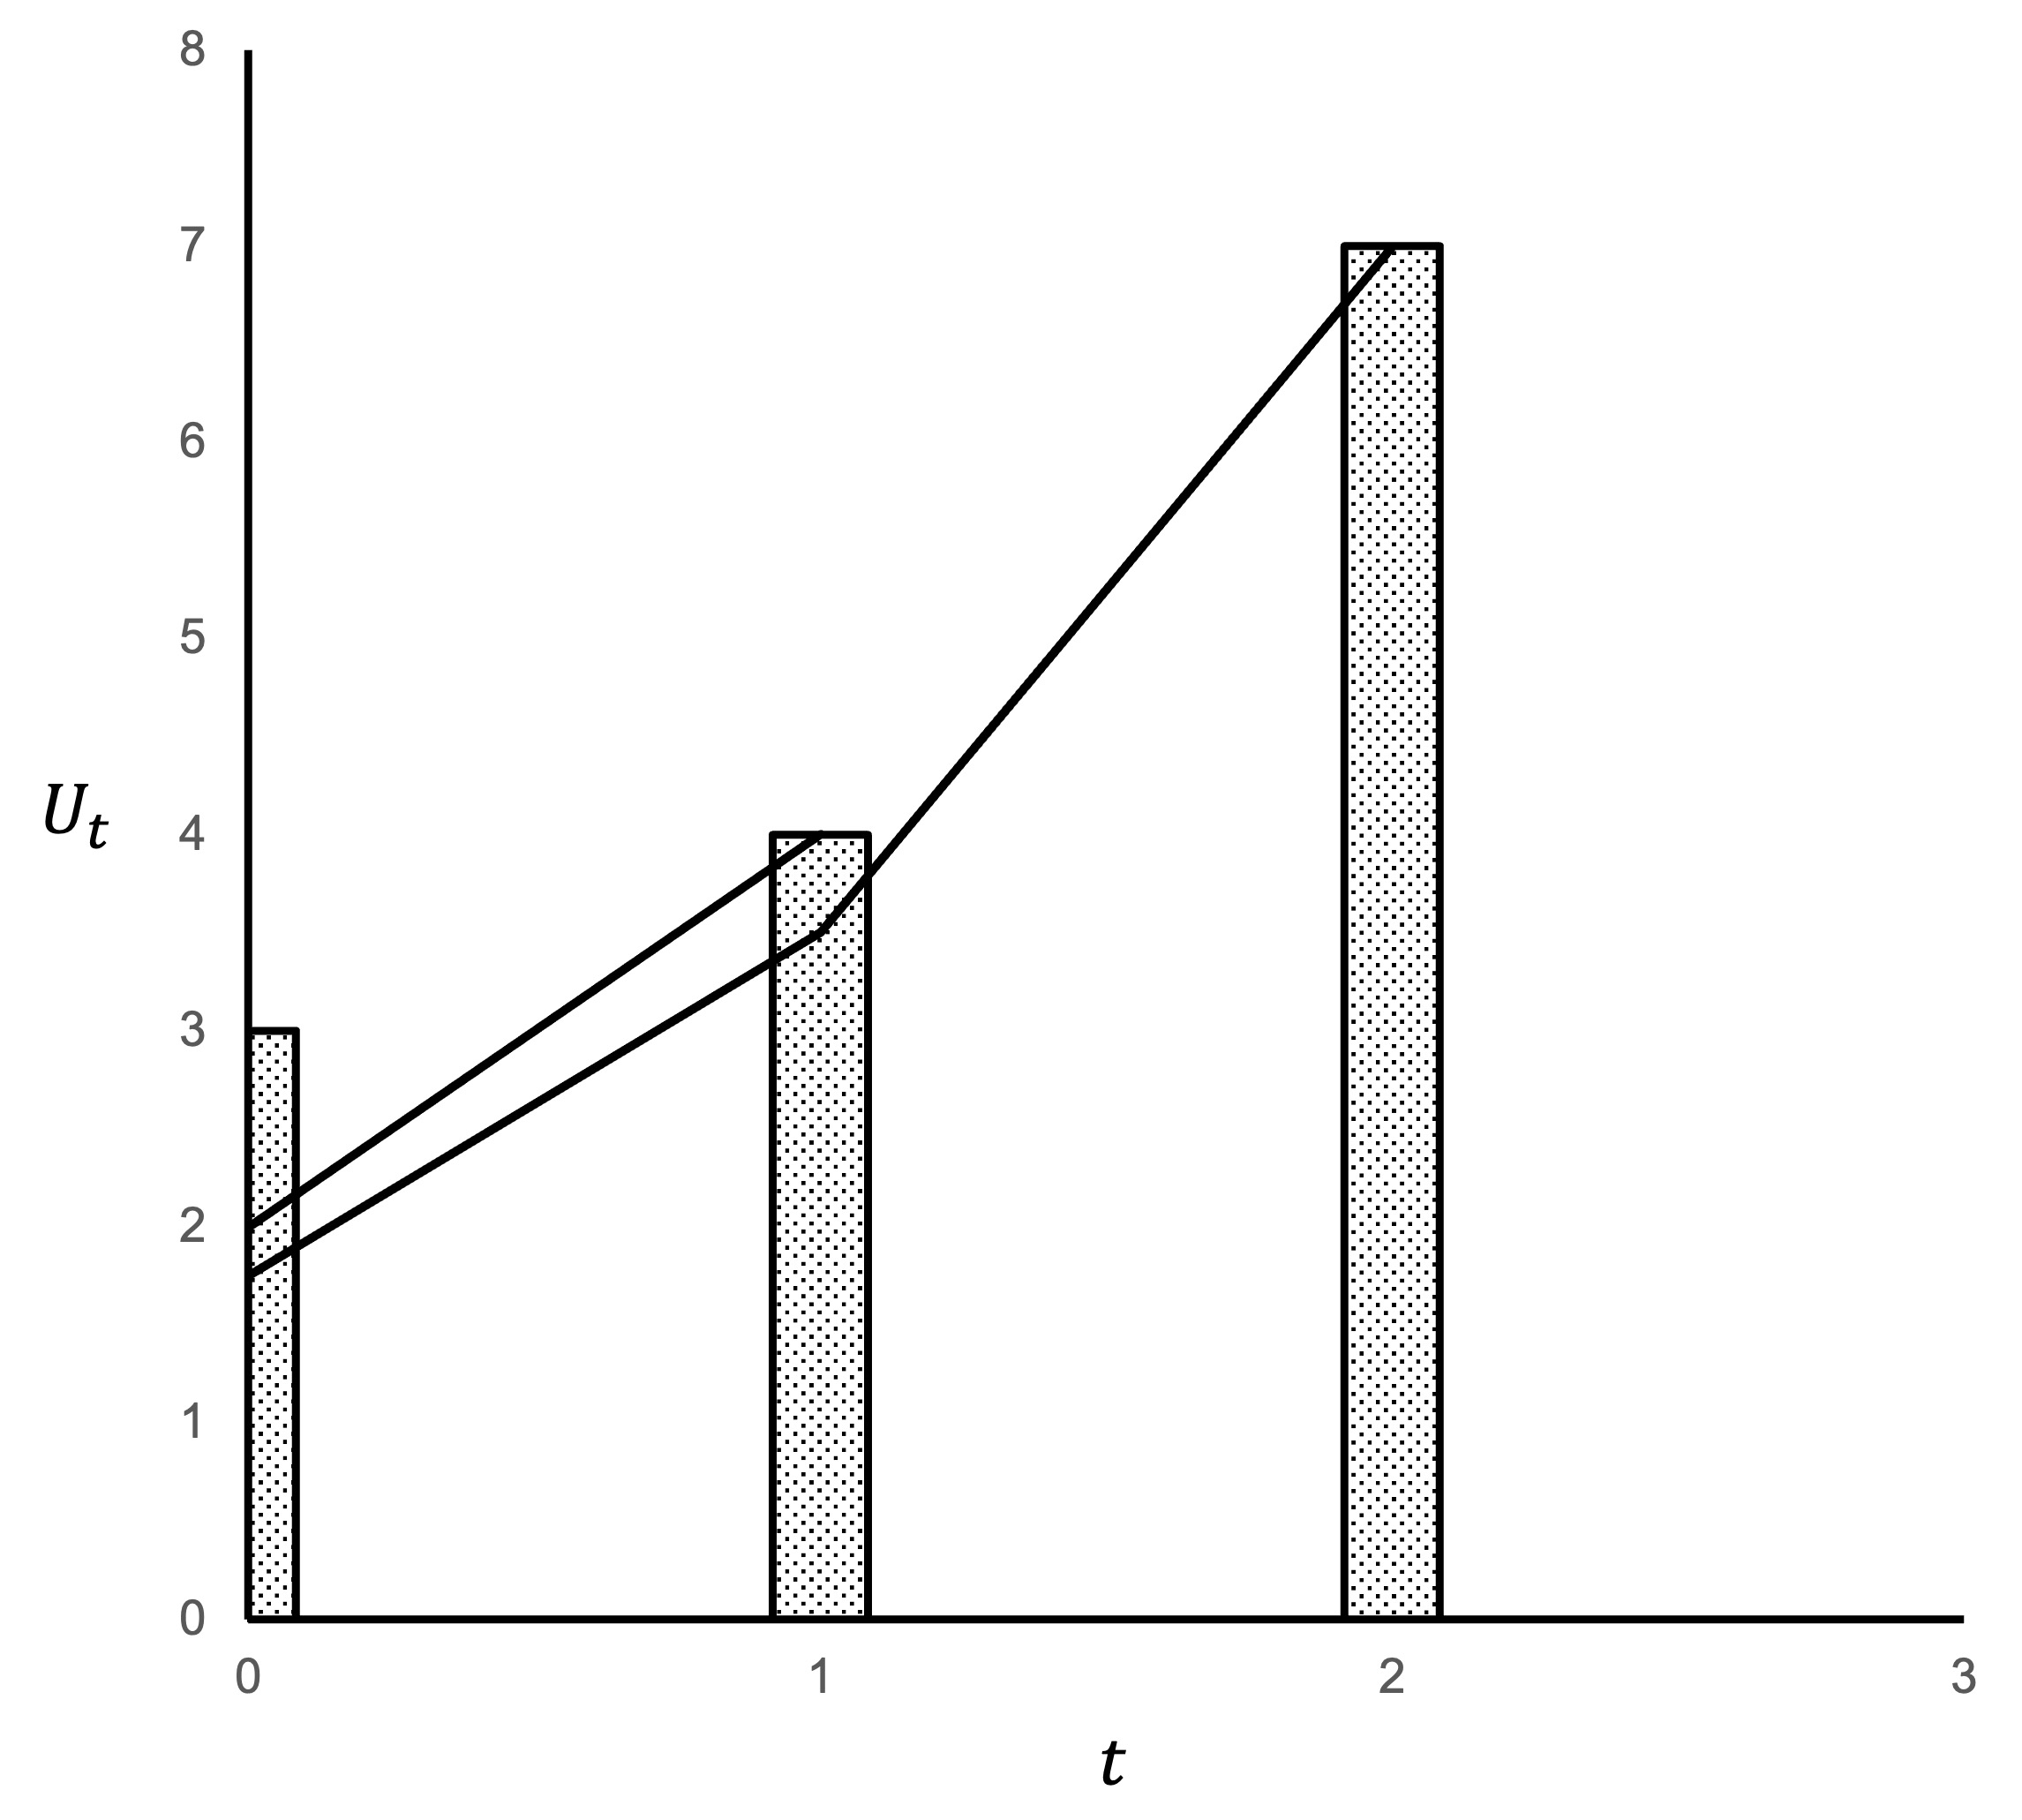
\includegraphics[width=0.5\textwidth,height=\textheight]{intertemporal-choice/img/Kate.jpg}

The below figure shows the each of the payoffs that Jack could receive
at \(t=0,1,2\). The lines represent the discounted utility of each
option at each time.

At \(t=0\) we can see that the \$4 paid at \(t=1\) gives higher
discounter utility. We can also see that the lines represented the
discounted utility at each time cross, giving the potential for a time
inconsistent decision.

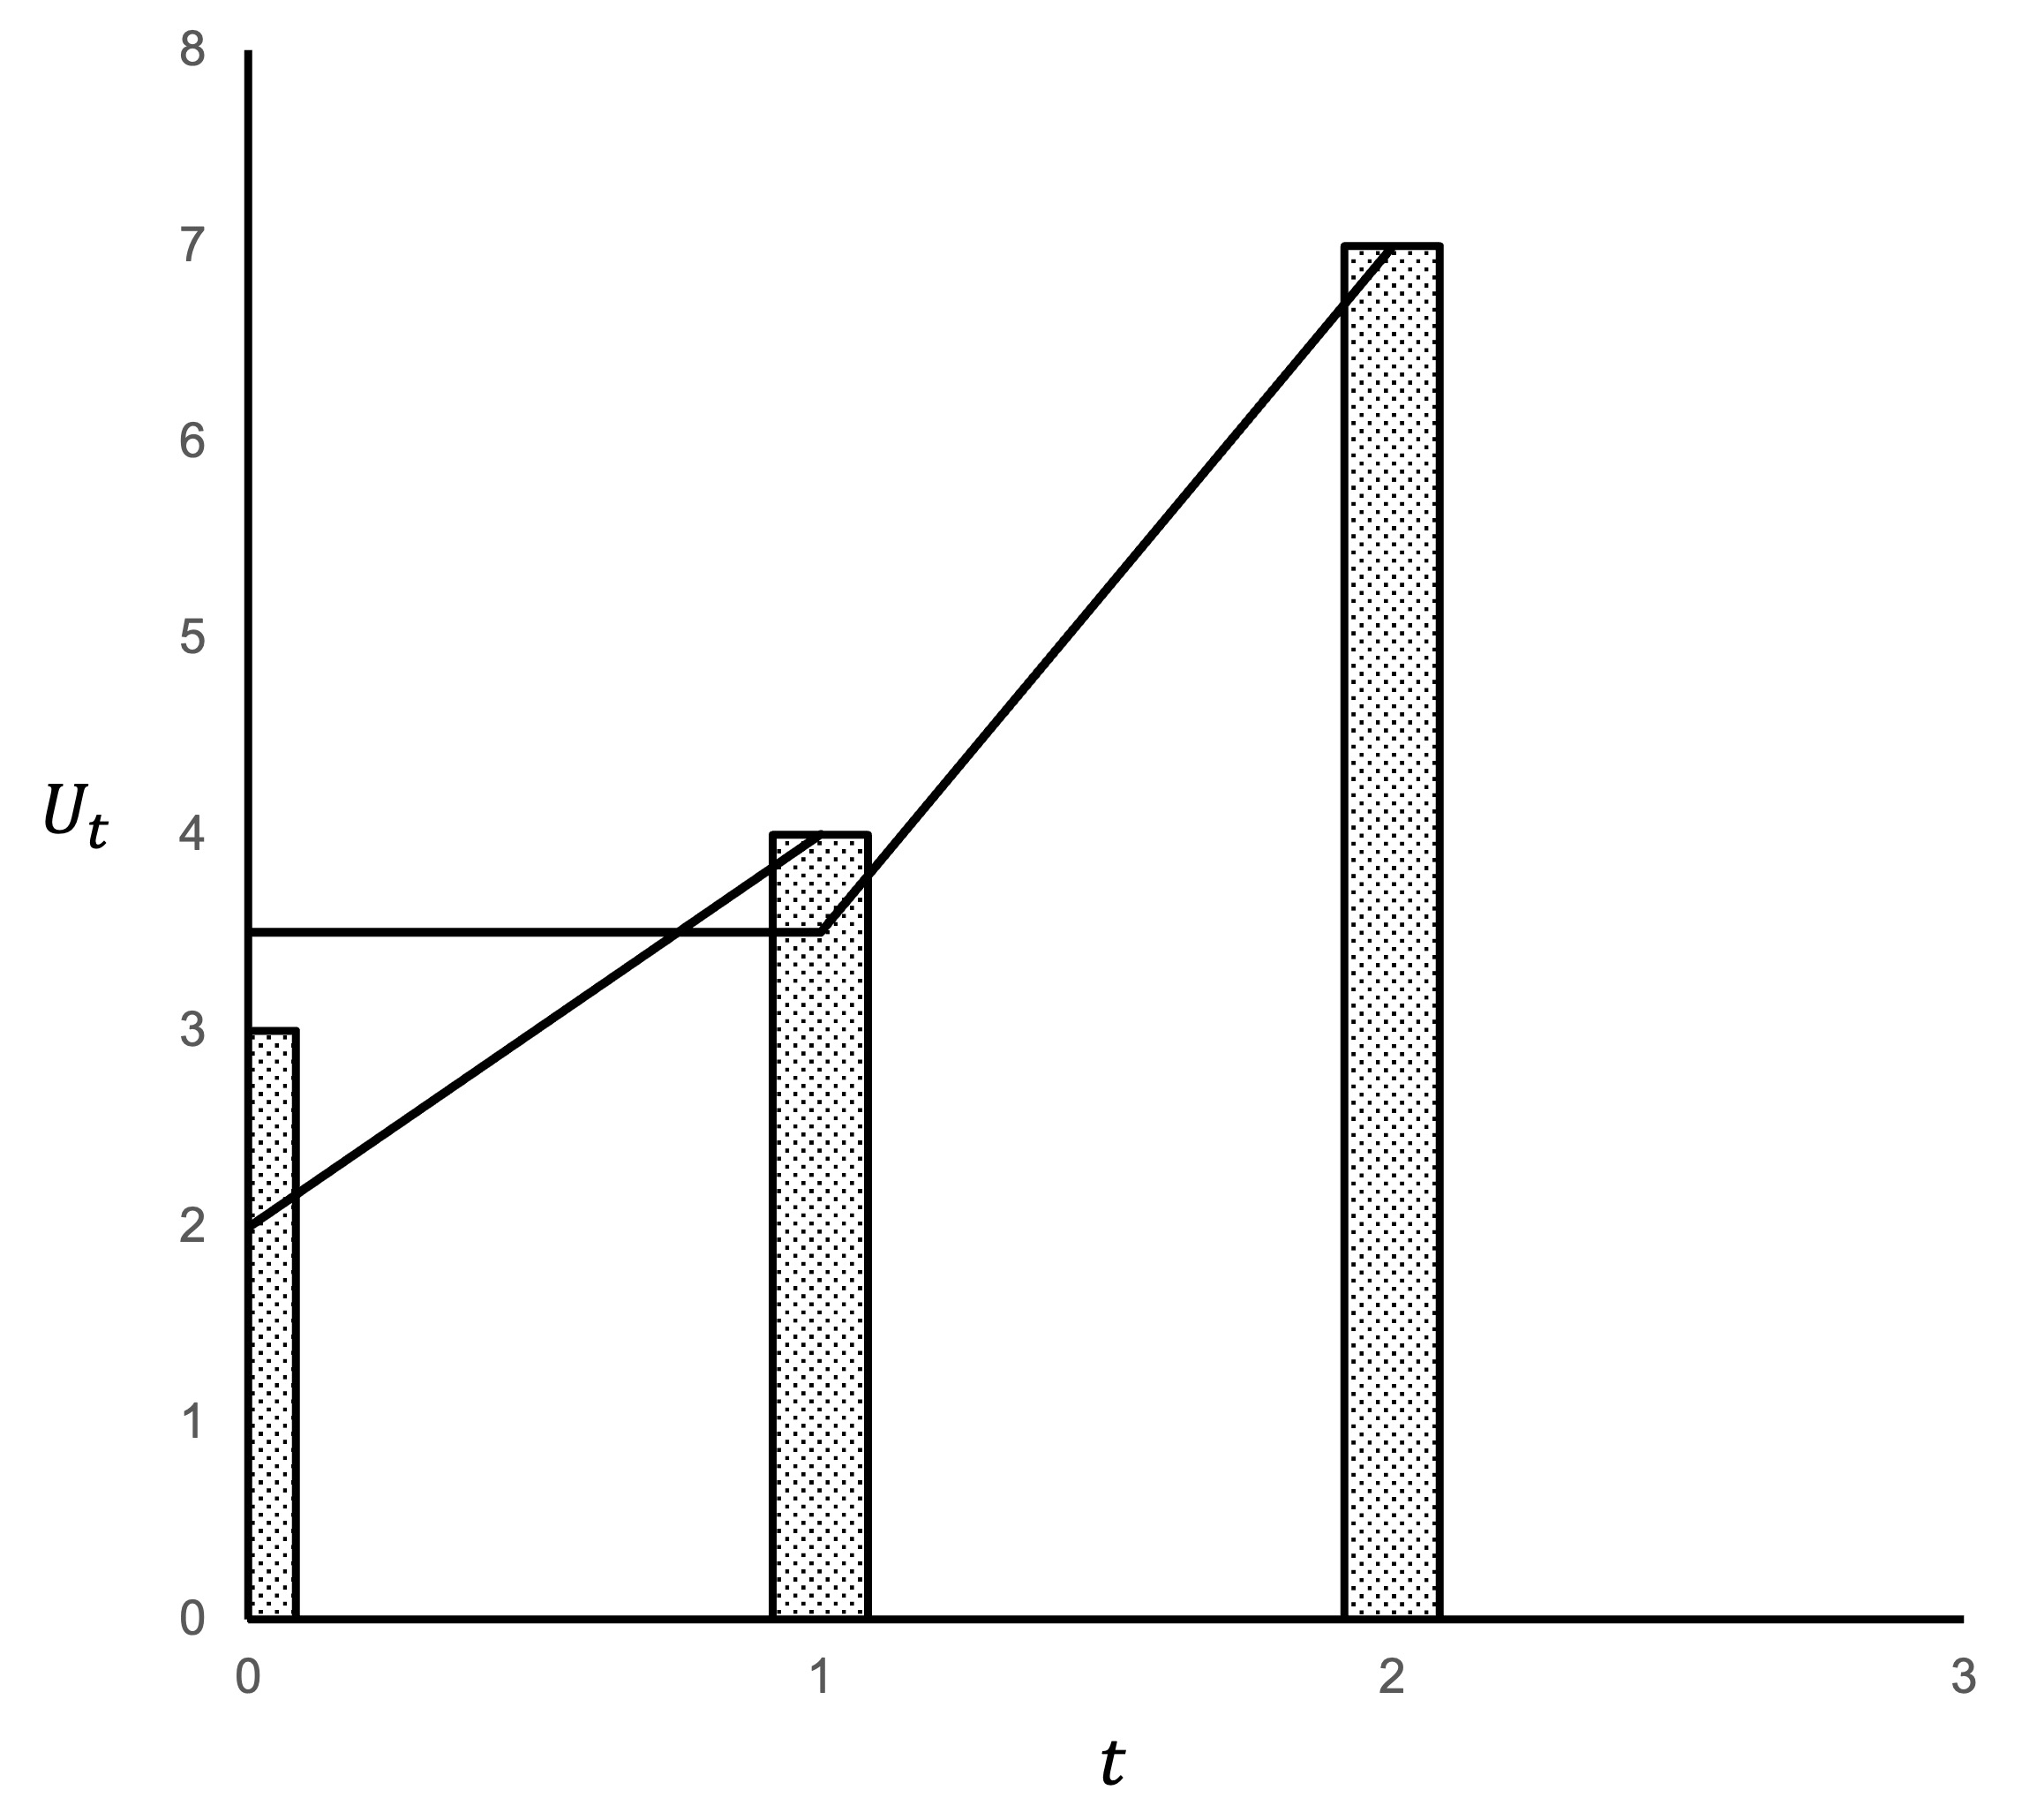
\includegraphics[width=0.5\textwidth,height=\textheight]{intertemporal-choice/img/Jack1.jpg}

In the next figure we move forward to \(t=1\). Jack's preferred option
changes. He now prefers the \$4 immediately. It is no longer discounted
by \(\beta\).

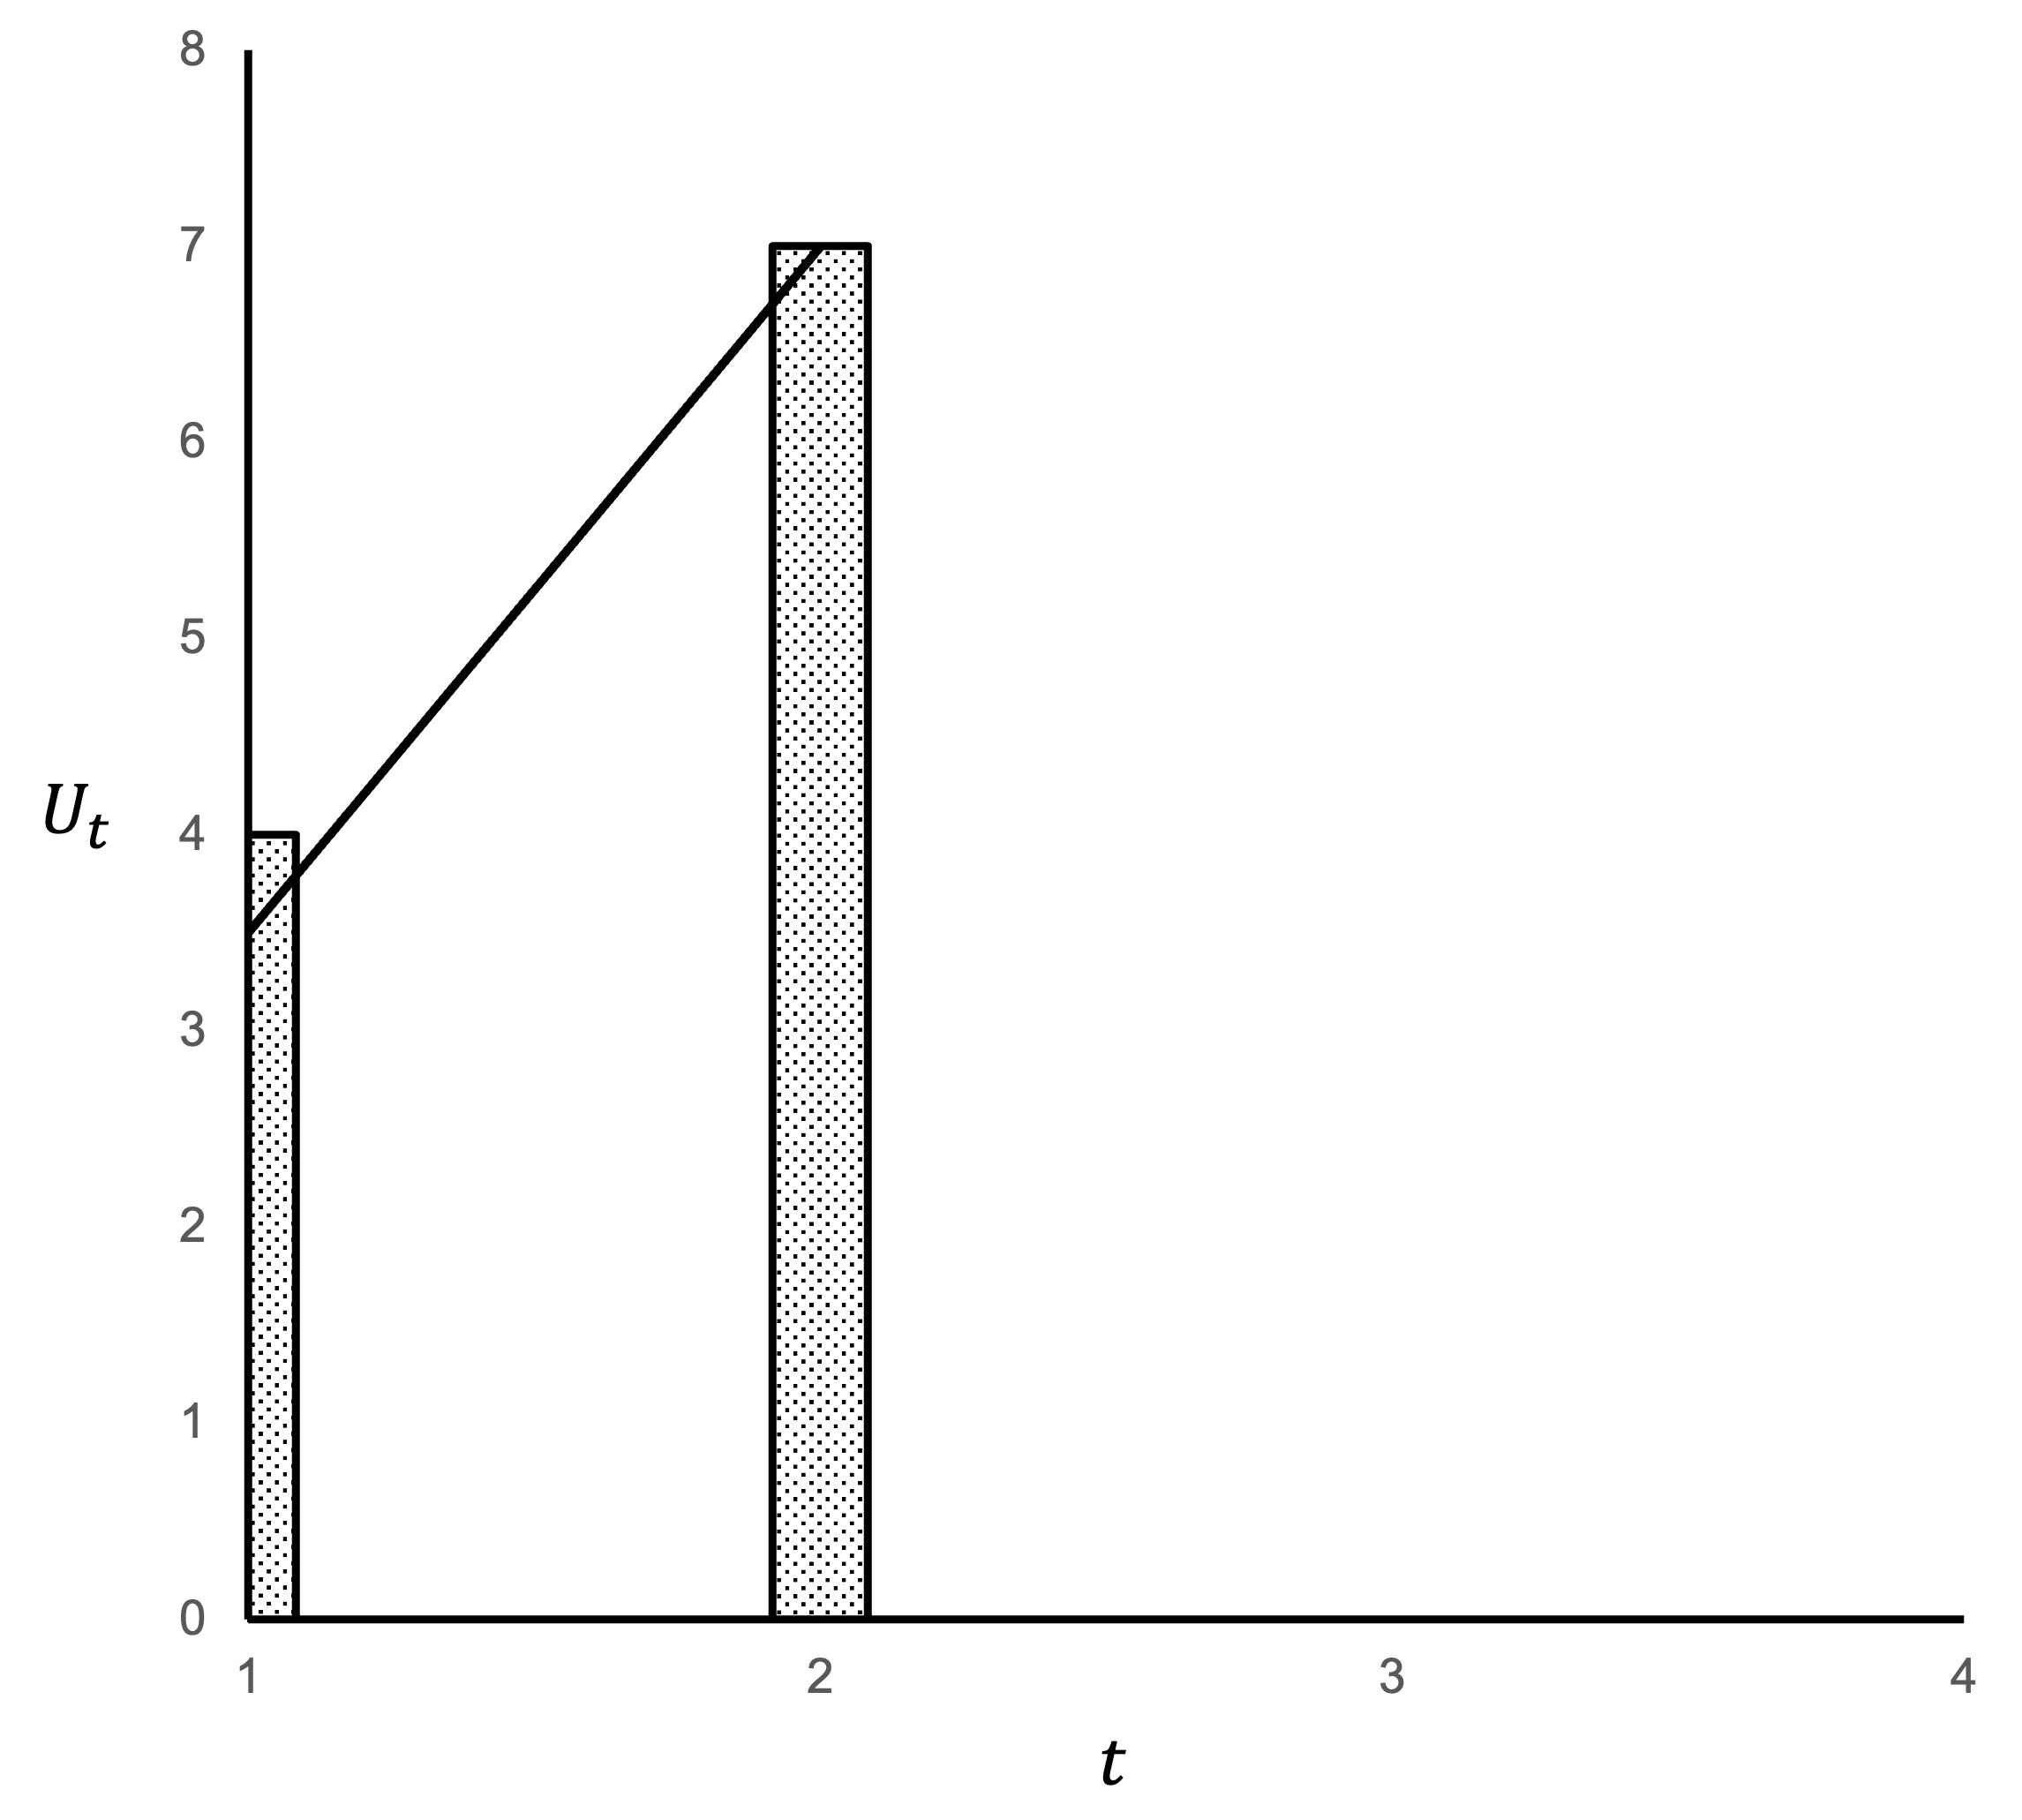
\includegraphics[width=0.5\textwidth,height=\textheight]{intertemporal-choice/img/Jack2.jpg}

\end{tcolorbox}

\hypertarget{small-reward-now-or-large-reward-later}{%
\section{Small reward now or large reward
later?}\label{small-reward-now-or-large-reward-later}}

a) Alfred and Blake are exponential discounters. They can choose between
a small reward now or a larger reward later. Alfred discounts the future
heavily (low \(\delta\)). Blake does not (\(\delta\) close to one).

How might Alfred and Blake's choices be affected by their discount
factor?

\begin{tcolorbox}[enhanced jigsaw, title=\textcolor{quarto-callout-tip-color}{\faLightbulb}\hspace{0.5em}{Answer}, toprule=.15mm, colback=white, breakable, titlerule=0mm, colframe=quarto-callout-tip-color-frame, coltitle=black, opacityback=0, rightrule=.15mm, colbacktitle=quarto-callout-tip-color!10!white, bottomtitle=1mm, opacitybacktitle=0.6, arc=.35mm, bottomrule=.15mm, toptitle=1mm, leftrule=.75mm, left=2mm]

Each will discount the two rewards, with the size of the discount for
the larger reward reflecting the size of the delay relative to the delay
for the small reward.

Alfred and Blake will prefer to wait if the discounted utility of the
larger reward is higher than that of the small reward.

As Alfred has a higher discount rate, Alfred is more likely than Blake
to prefer the small reward as Alfred will discount the larger reward by
more.

\end{tcolorbox}

b) Catherine is a quasi-hyperbolic discounter. She can choose between
the same two rewards. Before either award is available, she prefers the
large reward. However, she changes her mind and chooses when the small
reward at the time it becomes available.

Why did Catherine change her mind?

\begin{tcolorbox}[enhanced jigsaw, title=\textcolor{quarto-callout-tip-color}{\faLightbulb}\hspace{0.5em}{Answer}, toprule=.15mm, colback=white, breakable, titlerule=0mm, colframe=quarto-callout-tip-color-frame, coltitle=black, opacityback=0, rightrule=.15mm, colbacktitle=quarto-callout-tip-color!10!white, bottomtitle=1mm, opacitybacktitle=0.6, arc=.35mm, bottomrule=.15mm, toptitle=1mm, leftrule=.75mm, left=2mm]

If Catherine prefers the large reward, this means the discounted utility
of the larger reward is higher than that for the small reward. As both
rewards are experienced with delay, the small and large reward are
discounted by the short-term discount factor, plus the exponential
discount factor proportional to the delay.

When the small reward becomes available, Catherine no longer applies any
discount to the small reward. The exponential discount factor applied to
the larger reward also decreases for the time that has passed. Despite
the size of the exponential discount being applied to each reward
decreasing by the same amount, the removal of the short-term discount
factor from the small reward must have been of sufficient that it now
has the larger expected utility.

\end{tcolorbox}

\hypertarget{credit-score}{%
\section{Credit score}\label{credit-score}}

A credit score is a score developed by credit agencies and lenders as a
measure of how risky a borrower is. The score is derived using data on
past behaviour. A person with a higher credit score is considered more
likely to repay a loan on time.

Researchers found a correlation between people's discount factors,
\(\beta\) and \(\delta\), and their credit score.

What would this correlation be? Explain why you might see this
relationship.

\begin{tcolorbox}[enhanced jigsaw, title=\textcolor{quarto-callout-tip-color}{\faLightbulb}\hspace{0.5em}{Answer}, toprule=.15mm, colback=white, breakable, titlerule=0mm, colframe=quarto-callout-tip-color-frame, coltitle=black, opacityback=0, rightrule=.15mm, colbacktitle=quarto-callout-tip-color!10!white, bottomtitle=1mm, opacitybacktitle=0.6, arc=.35mm, bottomrule=.15mm, toptitle=1mm, leftrule=.75mm, left=2mm]

You would expect to see a positive correlation between the credit score
and the discount factors.

\(\beta\) relates to present-bias, which results in greater weight being
given to any costs or benefits today relative to costs and benefits
experienced with delay.

\(\delta\) relates to impatience, with each successive period of delay
being subject to a discount relative to the previous.

Both discount factors could affect the credit score.

To the extent the future is discounted due to either discount rate, this
makes borrowing more attractive provided the interest costs are not too
high.

If either discount factor were low enough, an agent might be willing to
borrow more than they could feasibly pay off in the future (or at
extortionate interest rates). The benefits of consumption today might
exceed the costs of failure to repay, with those costs sufficiently
discounted that them agent is willing to incur them. An agent with low
\(\beta\) might be particularly vulnerable to this as an impulsive
purchase today might be attractive even though the debt (e.g.~credit
card) might be payable soon. Failure to pay would hurt their credit
score.

Unintended payment problems are more likely to be caused by low
\(\beta\).

If someone with low \(\delta\) borrowed money with the intention to pay
it off in the future, they would stick to that plan. They are time
consistent.

Someone with low \(\beta\) may borrow with the intention to pay it off.
However, when the day of payment arrives, they may change their mind and
prefer not to incur the immediate cost of payment as that exceeds the
discounted costs in the future (such as penalty interest and a low
credit score). This would also hurt their credit score.

\end{tcolorbox}

\hypertarget{time-inconsistent-preferences}{%
\section{Time inconsistent
preferences}\label{time-inconsistent-preferences}}

Recall the question in Section~\ref{sec-Q3}.

We found that at \(t=0\) Jack planned to wait until tonight (\(t=2\))
for the \$7, but in the afternoon (\(t=1\)) he changed his mind and took
the \$4 that was available immediately.

Jack's friend Allan is a sophisticated quasi-hyperbolic discounter with
\(\beta=\frac{1}{2}\) and \(\delta=1\).

Does your answer change for Allan? Why?

\begin{tcolorbox}[enhanced jigsaw, title=\textcolor{quarto-callout-tip-color}{\faLightbulb}\hspace{0.5em}{Answer}, toprule=.15mm, colback=white, breakable, titlerule=0mm, colframe=quarto-callout-tip-color-frame, coltitle=black, opacityback=0, rightrule=.15mm, colbacktitle=quarto-callout-tip-color!10!white, bottomtitle=1mm, opacitybacktitle=0.6, arc=.35mm, bottomrule=.15mm, toptitle=1mm, leftrule=.75mm, left=2mm]

The behaviour of Jack that we observed in Tutorial 5 was that of a naive
hyperbolic discounter. In each period he calculated his preferred option
and acted as though he would stick to that decision in the future. He
did not anticipate changing his mind at \(t=1\).

Allan considers the choice by using backward induction from the final
period.

If Allan waits until tonight, he takes the \$7 with certainty.

Now considering his choice at \(t=1\).

\begin{align*}
U_1(\$4\text{ at }t=1)&=4 \\
U_1(\$7\text{ at }t=2)&=\beta\delta\times 7 \\
&=3.5
\end{align*}

At \(t=1\) Allan can see that he will cave in take the \$4.

Allan now considers \(t=0\) with the knowledge he will take the \$4 at
\(t=1\). He knows that he will not make it to the \$7 at \(t=2\), so he
removes it from his choice set.

\begin{align*}
U_0(\$3\text{ at }t=0)&=3 \\
U_0(\$4\text{ at }t=1)&=\beta\delta\times 4 \\
&=2
\end{align*}

At \(t=0\) Allan chooses the \$3. His sophistication leads him to
preproperate. He takes a lower amount earlier than the naive Jack.

\end{tcolorbox}

\hypertarget{eating-cake}{%
\section{Eating cake}\label{eating-cake}}

Kelvin and Linda both like chocolate cake. There are two periods in
which they can eat cake, \(t=1,2\). They receive an immediate benefit of
12 for eating cake at \(t=1\) and 6 for eating cake at \(t=2\)

At \(t=3\) they incur the costs of their diet and pay a cost of \(8\).
The total cost depends on how much cake they eat.

Kelvin and Linda have preferences of \(\beta=0.5\) and \(\delta=1\).

To illustrate, if Kelvin or Linda eat at \(t=1\) they receive a benefit
of \(12\) at \(t=1\) and a cost of \(8\) at \(t=3\). If Kelvin or Linda
eat at both at \(t=1\) and at \(t=2\), they receive a benefit of \(12\)
at \(t=1\) and \(6\) at \(t=2\) and a cost of \(16\) at \(t=3\).

Kelvin is naive, Linda is sophisticated.

a) When will Kelvin eat?

\begin{tcolorbox}[enhanced jigsaw, title=\textcolor{quarto-callout-tip-color}{\faLightbulb}\hspace{0.5em}{Answer}, toprule=.15mm, colback=white, breakable, titlerule=0mm, colframe=quarto-callout-tip-color-frame, coltitle=black, opacityback=0, rightrule=.15mm, colbacktitle=quarto-callout-tip-color!10!white, bottomtitle=1mm, opacitybacktitle=0.6, arc=.35mm, bottomrule=.15mm, toptitle=1mm, leftrule=.75mm, left=2mm]

We can calculate utility of eating in each round separately as the
utilities are additive.

At \(t=0\):

\begin{align*}
U_0(\text{eat at }t=1)&=\beta\delta\times 12-\beta\delta^3\times 8 \\
&=0.5\times 1\times 12-0.5\times 1^3 \times 8 \\
&=2 \\
\\
U_0(\text{eat at } t=2)&=\beta\delta^2\times 6-\beta\delta^3\times 8 \\
&=0.5\times 1^2\times 6-0.5\times 1^3 \times 8 \\
&=-1 
\end{align*}

Kelvin plans to eat at \(t=1\) but not \(t=2\).

At \(t=1\):

\begin{align*}
U_1(\text{eat at } t=1)&=12-\beta\delta^2\times 8 \\
&=12-0.5\times 1^2 \times 8 \\
&=8 \\
\\
U_1(\text{eat at } t=2)&=\beta\delta\times 6-\beta\delta^2\times 8 \\
&=0.5\times 1\times 6-0.5\times 1 \times 8 \\
&=-1 
\end{align*}

Kelvin eats at \(t=1\) but does not plan to eat at \(t=2\).

At \(t=2\):

\begin{align*}
U_2(\text{eat at } t=2)&=6-\beta\delta^2\times 8 \\
&=6-0.5\times 1^2 \times 8 \\
&=2 
\end{align*}

Kelvin eats at \(t=2\).

Kelvin, being naive, thinks he will stick to his initial plan of eating
at \(t=1\) but not at \(t=2\), but ends up eating in both periods.

\end{tcolorbox}

b) When will Linda eat?

\begin{tcolorbox}[enhanced jigsaw, title=\textcolor{quarto-callout-tip-color}{\faLightbulb}\hspace{0.5em}{Answer}, toprule=.15mm, colback=white, breakable, titlerule=0mm, colframe=quarto-callout-tip-color-frame, coltitle=black, opacityback=0, rightrule=.15mm, colbacktitle=quarto-callout-tip-color!10!white, bottomtitle=1mm, opacitybacktitle=0.6, arc=.35mm, bottomrule=.15mm, toptitle=1mm, leftrule=.75mm, left=2mm]

Linda is sophisticated and solves their problem backward.

There is no decision to make at \(t=3\). She simply incurs the cost of
their past behaviour.

At \(t=2\):

\begin{align*}
U_2(\text{eat at } t=2)&=6-\beta\delta^2\times 8 \\
&=6-0.5\times 1^2 \times 8 \\
&=2
\end{align*}

Linda anticipates that she will eat at \(t=2\).

Linda knows she will eat at \(t=2\), so she don't need to reconsider her
plan for then at \(t=1\).

At \(t=1\)

\begin{align*}
U_1(\text{eat at } t=1)&=12-\beta\delta^2\times 8 \\
&=12-0.5\times 1^2 \times 8 \\
&=8
\end{align*}

Linda also anticipates that she will eat at \(t=1\).

At \(t=0\), Linda can now see that she will eat at \(t=1\) and \(t=2\)
no matter what she decides now. She simply accepts her future course of
action.

\end{tcolorbox}

c) Assume that Kelvin and Linda can pay price \(p\) at \(t=0\) for a
binding commitment device that prevents them from eating more than they
initially plan. Assuming costs and benefits are measured in dollars,
what is the maximum price \(p\) that Linda would pay to use the
commitment device?

\begin{tcolorbox}[enhanced jigsaw, title=\textcolor{quarto-callout-tip-color}{\faLightbulb}\hspace{0.5em}{Answer}, toprule=.15mm, colback=white, breakable, titlerule=0mm, colframe=quarto-callout-tip-color-frame, coltitle=black, opacityback=0, rightrule=.15mm, colbacktitle=quarto-callout-tip-color!10!white, bottomtitle=1mm, opacitybacktitle=0.6, arc=.35mm, bottomrule=.15mm, toptitle=1mm, leftrule=.75mm, left=2mm]

From the perspective of period \(t=0\) all costs and benefits are
discounted. At \(t=0\):

\begin{align*}
U_0(\text{eat at } t=1)&=\beta\delta\times 12-\beta\delta^3\times 8 \\
&=0.5\times 1\times 12-0.5\times 1^3 \times 8 \\
&=2 \\
\\
U_0(\text{eat at } t=2)&=\beta\delta^2\times 12-\beta\delta^3\times 8 \\
&=0.5\times 1^2\times 6-0.5\times 1^3 \times 8 \\
&=-1 
\end{align*}

From the perspective of \(t=0\), eating at \(t=2\) has negative
discounted utility. As a result, if a commitment device available, Linda
would use it to commit to not eating at \(t=2\). The commitment device
would prevent a loss of \(1\). Therefore, Linda would pay up to
\(p=\$1\).

\end{tcolorbox}

d) What happens to Kelvin, a naive agent, in the presence of the
commitment device?

\begin{tcolorbox}[enhanced jigsaw, title=\textcolor{quarto-callout-tip-color}{\faLightbulb}\hspace{0.5em}{Answer}, toprule=.15mm, colback=white, breakable, titlerule=0mm, colframe=quarto-callout-tip-color-frame, coltitle=black, opacityback=0, rightrule=.15mm, colbacktitle=quarto-callout-tip-color!10!white, bottomtitle=1mm, opacitybacktitle=0.6, arc=.35mm, bottomrule=.15mm, toptitle=1mm, leftrule=.75mm, left=2mm]

Being naive, Kelvin does not perceive the necessity of using a
commitment device as he trusts he will comply with his plans.

\end{tcolorbox}

\hypertarget{completing-an-assignment}{%
\section{Completing an assignment}\label{completing-an-assignment}}

Your assignment is due today at \(t=0\).

You can complete the assignment within a day, but on that day you will
incur a utility cost of 10.

For every day you submit late, you lose one mark. You experience a
utility cost of 1 for every mark lost \textbf{on the day it is lost}. If
handed in more than 6 days late, you will fail and experience utility
cost of 1000. (In other words, if you haven't yet submitted, you will
definitely submit at \(t=6\)).

This leaves you with a decision to hand in at
\(t = 0, t = 1, t = 2, ... , t = 5\), or \(t=6\).

For instance:

\begin{itemize}
\tightlist
\item
  If you submit today, at \(t=0\), you experience utility cost of 10.
\item
  If you submit tomorrow, at \(t=1\), you will experience utility cost
  of 10 plus a utility cost of 1 for the mark lost on that day.
\item
  If you submit at \(t=2\), you will experience a utility cost of 1 at
  \(t=1\) for the mark lost, a utility cost of 1 at \(t=2\) for another
  mark lost, and a utility cost of 10 for completing the assignment.
\item
  If you submit at \(t=6\), you will experience a utility cost of 1 on
  each day from \(t=1\) to \(t=6\) for the marks lost, plus a utility
  cost of 10 at \(t=6\) for completing the assignment.
\end{itemize}

You are a hyperbolic discounter with \(\beta=0.75\) and \(\delta=1\).

a) When do you finish if you are naive?

\begin{tcolorbox}[enhanced jigsaw, title=\textcolor{quarto-callout-tip-color}{\faLightbulb}\hspace{0.5em}{Answer}, toprule=.15mm, colback=white, breakable, titlerule=0mm, colframe=quarto-callout-tip-color-frame, coltitle=black, opacityback=0, rightrule=.15mm, colbacktitle=quarto-callout-tip-color!10!white, bottomtitle=1mm, opacitybacktitle=0.6, arc=.35mm, bottomrule=.15mm, toptitle=1mm, leftrule=.75mm, left=2mm]

At \(t=0\) you have 7 possible plans to consider: finishing your
assignment at \(t=0\) through to \(t=6\). You compare the discounted
utilities from the various plans as follows.

At \(t=0\):

\begin{itemize}
\tightlist
\item
  Finish today (\(t=0\)): \(-10\)
\item
  Finish tomorrow (\(t=1\)): \(0.75(-10-1)=-8.50\)
\item
  Finish at \(t=2\): \(0.75(-10-2)=-9.25\)
\item
  Finish at \(t=3\): \(0.75(-10-3)=-10\)
\item
  \ldots{}
\item
  Finish at \(t=6\): \(0.75(-10-6)=-12\)
\end{itemize}

At \(t=0\), you plan to finish at \(t=1\) as that yields the highest
discounted utility. You put off finishing the assignment until tomorrow.

At \(t=1\) you then reconsider your decision. The penalty received at
\(t=1\) is now sunk and won't affect the decision:

\begin{itemize}
\tightlist
\item
  Finish today (\(t=1\)): \(-10=-10\)
\item
  Finish tomorrow (\(t=2\)): \(0.75(-10-1)=-8.25\)
\item
  Finish at \(t=3\): \(0.75(-10-2)=-9\)
\item
  \ldots{}
\item
  Finish at \(t=6\): \(0.75(-10-5)=-11.25\)
\end{itemize}

At \(t=1\), you change your plan and now intend to finish at \(t=2\),
which yields the highest discounted utility.

This pattern continues day after day, always intending to complete
tomorrow, until \(t=6\), with an ultimate outcome of -10 utility cost on
that day, plus -1 utility cost each day for the last 6 days.

\begin{itemize}
\tightlist
\item
  Finish at \(t=5\): \(-10\)
\item
  Finish at \(t=6\): \(0.75(-10-1)=-8.25\)
\end{itemize}

\end{tcolorbox}

b) When do you finish if you are sophisticated?

\begin{tcolorbox}[enhanced jigsaw, title=\textcolor{quarto-callout-tip-color}{\faLightbulb}\hspace{0.5em}{Answer}, toprule=.15mm, colback=white, breakable, titlerule=0mm, colframe=quarto-callout-tip-color-frame, coltitle=black, opacityback=0, rightrule=.15mm, colbacktitle=quarto-callout-tip-color!10!white, bottomtitle=1mm, opacitybacktitle=0.6, arc=.35mm, bottomrule=.15mm, toptitle=1mm, leftrule=.75mm, left=2mm]

If you are sophisticated, you will start at the end and work backwards.

At \(t=6\), you know that if you haven't finished the assignment you
must, with -10 utility.

At \(t=5\), you choose between:

\begin{itemize}
\tightlist
\item
  Finish at \(t=5\): \(-10\)
\item
  Finish at \(t=6\): \(0.75(-10-1)=-8.25\)
\end{itemize}

You do not plan to do the assignment at \(t=5\) and you remove \(t=5\)
from your plans.

At \(t=4\), you choose between:

\begin{itemize}
\tightlist
\item
  Finish at \(t=4\): \(-10\)
\item
  Finish at \(t=6\): \(0.75(-10-2)=-9\)
\end{itemize}

You do not plan to do the assignment at \(t=4\) and you remove \(t=4\)
from your plans.

At \(t=3\), you choose between:

\begin{itemize}
\tightlist
\item
  Finish at \(t=3\): \(-10\)
\item
  Finish at \(t=6\): \(0.75(-10-3)=-9.75\)
\end{itemize}

You do not plan to do the assignment at \(t=3\) and you remove \(t=3\)
from your plans.

At \(t=2\), you choose between:

\begin{itemize}
\tightlist
\item
  Finish at \(t=2\): \(-10\)
\item
  Finish at \(t=6\): \(0.75(-10-4)=-10.5\)
\end{itemize}

Utility is higher completing the assignment earlier. You plan to do the
assignment at \(t=2\) and you remove \(t=6\) from your plans.

At \(t=1\), you choose between:

\begin{itemize}
\tightlist
\item
  Finish at \(t=1\): \(-10\)
\item
  Finish at \(t=2\): \(0.75(-10-1)=-8.25\)
\end{itemize}

You plan to do the assignment at \(t=2\) and you remove \(t=1\) from
your plans.

At \(t=0\), you choose between:

\begin{itemize}
\tightlist
\item
  Finish at \(t=0\): \(-10\)
\item
  Finish at \(t=2\): \(0.75(-10-2)=-9\)
\end{itemize}

You will not change your intentions further and will complete the
assignment at \(t=2\).

\end{tcolorbox}

\hypertarget{saving-for-retirement}{%
\section{Saving for retirement}\label{saving-for-retirement}}

Citizens of Perthia have the choice between the following options:

\begin{itemize}
\tightlist
\item
  Saving for retirement at \(t=1\) (\(u_1=0\)) and having a comfortable
  retirement at \(t=2\) (\(u_2=20\))
\item
  Spending at \(t=1\) (\(u_1=10\)) and having a difficult retirement at
  \(t=2\) (\(u_2=0\)).
\end{itemize}

a) Ellie is an exponential discounter with \(\delta=3/4\). What does
Ellie choose at \(t=0\) and \(t=1\)? Why?

\begin{tcolorbox}[enhanced jigsaw, title=\textcolor{quarto-callout-tip-color}{\faLightbulb}\hspace{0.5em}{Answer}, toprule=.15mm, colback=white, breakable, titlerule=0mm, colframe=quarto-callout-tip-color-frame, coltitle=black, opacityback=0, rightrule=.15mm, colbacktitle=quarto-callout-tip-color!10!white, bottomtitle=1mm, opacitybacktitle=0.6, arc=.35mm, bottomrule=.15mm, toptitle=1mm, leftrule=.75mm, left=2mm]

\begin{align*}
U_0(save)&=\delta u_1+\delta^2 u_2 \\
&=0+\bigg(\frac{3}{4}\bigg)^2\times 20 \\
&=11.25 \\
\\
U_0(spend)&=\delta u_1+\delta^2 u_2 \\
&=\frac{3}{4}\times 10+0 \\
&=7.5 \\
\\
U_1(save)&=u_1+\delta u_2 \\
&=0+\frac{3}{4}\times 20 \\
&=15 \\
\\
U_1(spend)&=u_1+\delta u_2 \\
&=10+0\\
&=10
\end{align*}

Ellie intends to save in both periods and does so. Ellie is time
consistent. Knowing that Ellie is an exponential discounter, we did not
need to calculate her decision at both \(t=0\) and \(t=1\). As
exponential discounters are time consistent, we could have simply
determined her decision for one period and known that would also be her
decision at other times.

\end{tcolorbox}

b) Freddie is a naive quasi-hyperbolic discounter with \(\beta=1/4\) and
\(\delta=1\). What does Freddie choose at \(t=0\) and \(t=1\)? Why?

\begin{tcolorbox}[enhanced jigsaw, title=\textcolor{quarto-callout-tip-color}{\faLightbulb}\hspace{0.5em}{Answer}, toprule=.15mm, colback=white, breakable, titlerule=0mm, colframe=quarto-callout-tip-color-frame, coltitle=black, opacityback=0, rightrule=.15mm, colbacktitle=quarto-callout-tip-color!10!white, bottomtitle=1mm, opacitybacktitle=0.6, arc=.35mm, bottomrule=.15mm, toptitle=1mm, leftrule=.75mm, left=2mm]

\begin{align*}
U_0(save)&=\beta\delta u_1+\beta\delta^2 u_2 \\
&=0+\frac{1}{4}\times (1)^2\times 20 \\
&=5 \\
\\
U_0(spend)&=\beta\delta u_1+\beta\delta^2 u_2 \\
&=\frac{1}{4}\times 1\times 10+0 \\
&=2.5 \\
\end{align*}

At \(t=0\) Freddie plans to save.

\begin{align*}
U_1(save)&=u_1+\beta\delta u_2 \\
&=0+\frac{1}{4}\times 1\times 20 \\
&=5 \\
\\
U_1(spend)&=u_1+\beta\delta u_2 \\
&=10+0 \\
&=10
\end{align*}

At \(t=1\) Freddie chooses to spend Freddie has changed his mind. He is
time inconsistent. At \(t=0\) both saving and spending are subject to
the short-term discount factor \(\beta\), with the relative discount
between saving and spending being only \(\delta\). However, at \(t=1\)
the benefit of spending is available immediately and no longer
discounted by \(\beta\).

\end{tcolorbox}

c) Grant is a sophisticated quasi-hyperbolic discounter with
\(\beta=1/4\) and \(\delta=1\). What does Grant do? Why?

\begin{tcolorbox}[enhanced jigsaw, title=\textcolor{quarto-callout-tip-color}{\faLightbulb}\hspace{0.5em}{Answer}, toprule=.15mm, colback=white, breakable, titlerule=0mm, colframe=quarto-callout-tip-color-frame, coltitle=black, opacityback=0, rightrule=.15mm, colbacktitle=quarto-callout-tip-color!10!white, bottomtitle=1mm, opacitybacktitle=0.6, arc=.35mm, bottomrule=.15mm, toptitle=1mm, leftrule=.75mm, left=2mm]

Grant works through his options using backward induction.

At \(t=2\) Grant has no decision to make.

At \(t=1\):

\begin{align*}
U_1(save)&=u_1+\beta\delta u_2 \\
&=0+\frac{1}{4}\times 1\times 20 \\
&=5 \\
\\
U_1(spend)&=u_1+\beta\delta u_2 \\
&=10+0\\
&=10
\end{align*}

At \(t=1\) Grant will spend. (This is the same calculation we made for
Freddie at \(t=1\).)

As Grant knows he will spend at \(t=1\), that is the only feasible
option available at \(t=0\). Grant will choose to spend.

Ultimately, Grant takes the same action as Freddie. However, he can see
his future decisions and is aware of that coming failure to stick with
what would be his preferences at \(t=0\).

\end{tcolorbox}

d) Grant is offered the opportunity to bind himself to a course of
action at \(t=0\) at the cost of 1 point of utility at \(t=2\). What
does Grant do?

\begin{tcolorbox}[enhanced jigsaw, title=\textcolor{quarto-callout-tip-color}{\faLightbulb}\hspace{0.5em}{Answer}, toprule=.15mm, colback=white, breakable, titlerule=0mm, colframe=quarto-callout-tip-color-frame, coltitle=black, opacityback=0, rightrule=.15mm, colbacktitle=quarto-callout-tip-color!10!white, bottomtitle=1mm, opacitybacktitle=0.6, arc=.35mm, bottomrule=.15mm, toptitle=1mm, leftrule=.75mm, left=2mm]

In the presence of the commitment device, Grant now has two feasible
options to consider at \(t=0\).

\begin{align*}
U_0(commit)&=\beta\delta u_1+\beta\delta^2 u_2 \\
&=0+\frac{1}{4}\times (1)^2\times (20-1) \\
&=4.75 \\
\\
U_0(spend)&=\beta\delta u_1+\beta\delta^2 u_2 \\
&=\frac{1}{4}\times 1\times 10+0 \\
&=2.5 \\
\end{align*}

Grant now chooses to commit at a price of one unit of utility at
\(t=2\).

\end{tcolorbox}

\hypertarget{work-or-party}{%
\section{Work or party?}\label{work-or-party}}

Ruby is a sophisticated present-biased agent with \(\beta=0.5\) and
\(\delta=1\). She has utility function \(u(x)=x\).

Ruby is deciding today (\(t=0\)) whether she will either:

\begin{itemize}
\tightlist
\item
  work tomorrow (\(t=1\)) for \$10 income to be received the day after
  she works (\(t=2\)) or
\item
  party tomorrow (\(t=1\)) for immediate utility of 8 but no income.
\end{itemize}

That is, she is deciding between (2, 10) and (1,8).

a) What does Ruby decide?

\begin{tcolorbox}[enhanced jigsaw, title=\textcolor{quarto-callout-tip-color}{\faLightbulb}\hspace{0.5em}{Answer}, toprule=.15mm, colback=white, breakable, titlerule=0mm, colframe=quarto-callout-tip-color-frame, coltitle=black, opacityback=0, rightrule=.15mm, colbacktitle=quarto-callout-tip-color!10!white, bottomtitle=1mm, opacitybacktitle=0.6, arc=.35mm, bottomrule=.15mm, toptitle=1mm, leftrule=.75mm, left=2mm]

Ruby is sophisticated, so uses backward induction to decide her
preferred course of action.

At \(t=2\) there is no decision to make. Ruby bears the consequences of
her earlier decisions.

At \(t=1\) she compares the discounted utility of the two options:

\begin{align*}
U_1(\text{work})&=\beta\delta u(\text{work}) \\
&=0.5\times 1\times 10 \\
&=5 \\
\\
U_1(\text{party})&=u(\text{party}) \\
&=8
\end{align*}

At \(t=1\) the discounted utility partying is higher than that of
working (\(U_1(\text{party})>U_1(\text{work})\)), so Penny prefers to
party.

At \(t=0\) Penny knows that she will party at \(t=1\) no matter what she
decides at \(t=0\), so she accepts that she will party.

\end{tcolorbox}

b) Ruby is able to commit to working at \(t=1\) by posting a letter at
\(t=0\) declining the party invitation (at no cost). Once she sends the
letter, she cannot change her mind. Will she decline the invitation?

\begin{tcolorbox}[enhanced jigsaw, title=\textcolor{quarto-callout-tip-color}{\faLightbulb}\hspace{0.5em}{Answer}, toprule=.15mm, colback=white, breakable, titlerule=0mm, colframe=quarto-callout-tip-color-frame, coltitle=black, opacityback=0, rightrule=.15mm, colbacktitle=quarto-callout-tip-color!10!white, bottomtitle=1mm, opacitybacktitle=0.6, arc=.35mm, bottomrule=.15mm, toptitle=1mm, leftrule=.75mm, left=2mm]

The presence of the commitment device allows Ruby to include the option
of working when she makes a decision at \(t=0\). She will now compare
the discounted utility of using the commitment device with the
discounted utility of working.

\begin{align*}
U_0(\text{commit+work})&=\beta\delta^2 u(\text{commit+work}) \\
&=0.5\times 1^2\times 10 \\
&=5 \\
\\
U_0(\text{party})&=\beta\delta u(\text{party}) \\
&=0.5\times 1\times 8 \\
&=4
\end{align*}

\(U_0(\text{commit+work})>U_0(\text{party})\), so Ruby commits to
working by declining the invitation.

\end{tcolorbox}

c) Suppose declining the party invitation comes at a cost to Ruby's
reputation at \(t=2\). What is the largest utility cost that Ruby would
be willing to incur such that she would still use the commitment device
of declining the invitation?

\begin{tcolorbox}[enhanced jigsaw, title=\textcolor{quarto-callout-tip-color}{\faLightbulb}\hspace{0.5em}{Answer}, toprule=.15mm, colback=white, breakable, titlerule=0mm, colframe=quarto-callout-tip-color-frame, coltitle=black, opacityback=0, rightrule=.15mm, colbacktitle=quarto-callout-tip-color!10!white, bottomtitle=1mm, opacitybacktitle=0.6, arc=.35mm, bottomrule=.15mm, toptitle=1mm, leftrule=.75mm, left=2mm]

The largest cost she would be willing to incur is the cost where the
discounted utility of each option is equal. Setting the cost as \(c\):

\begin{align*}
U_0(\text{commit})&=\beta\delta^2 u(\text{work}-c) \\
&=0.5\times 1^2\times (10-c) \\
&=5-0.5c \\
\\
U_0(\text{party})&=\beta\delta u(\text{party}) \\
&=0.5\times 1\times 8 \\
&=4
\end{align*}

Ruby will be indifferent where \(5-0.5c=4\) or where \(c=2\). The
largest utility cost she would be willing to incur is 2.

\end{tcolorbox}

d) Victoria is a naive present-biased agent with \(\beta=0.5\) and
\(\delta=1\). She has utility function \(u(x)=x\).

Victoria faces the same choice as Ruby and also has the chance to
decline at \(t=0\) the party invitation at a cost to Victoria's
reputation at \(t=2\). Will Victoria decline the invitation?

\begin{tcolorbox}[enhanced jigsaw, title=\textcolor{quarto-callout-tip-color}{\faLightbulb}\hspace{0.5em}{Answer}, toprule=.15mm, colback=white, breakable, titlerule=0mm, colframe=quarto-callout-tip-color-frame, coltitle=black, opacityback=0, rightrule=.15mm, colbacktitle=quarto-callout-tip-color!10!white, bottomtitle=1mm, opacitybacktitle=0.6, arc=.35mm, bottomrule=.15mm, toptitle=1mm, leftrule=.75mm, left=2mm]

As Victoria has the same discount function as Ruby, we know from
question b) that Victoria will decide to work at \(t=0\). We also know
from question a) that she will then change her mind and party at
\(t=1\).

However, as Victoria is naive she does not see her future self-control
problem and does not have the foresight to realise at \(t=0\) that she
will not work as planned. As a result, she would see no need in the
commitment device and would not be willing to incur any cost to use it.

\end{tcolorbox}

\hypertarget{buy-now-pay-later}{%
\section{Buy-now pay-later}\label{buy-now-pay-later}}

Buy-now pay-later works as follows: a person purchases an item with an
initial payment of one-quarter of the purchase price. They get access to
the purchased item immediately. They then pay three equal instalments
each fortnight until they have paid for the purchase in full. If they
fail to make a payment on time, they are required to pay a fee of \$10
and are barred from using the buy-now pay-later facility in the future.

Vernon used a buy-now pay-later provider to purchase a new jacket for
\$200. He paid \$50 on the day of the purchase and is now required to
pay the next \$50 instalment in two weeks. That is, Vernon's schedule of
costs and benefits is:

\begin{itemize}
\tightlist
\item
  Purchase date: Gains jacket and pays \$50
\item
  In two weeks: Pays \$50
\item
  In four weeks: Pays \$50
\item
  In six weeks: Pays \$50
\end{itemize}

At that time of the purchase Vernon intends to pay for the jacket as
required by the buy-now pay-later provider in two, four and six weeks.

Two weeks after the purchase when his payment became due Vernon changed
his mind and did not make the payment. He purchased a carton of beer for
a party that night with the money instead. Vernon's options and the cost
and benefits of those options had not changed since the purchase date.

Is Vernon an exponential discounter or present-biased? Why? Explain why
Vernon changed his mind.

\begin{tcolorbox}[enhanced jigsaw, title=\textcolor{quarto-callout-tip-color}{\faLightbulb}\hspace{0.5em}{Answer}, toprule=.15mm, colback=white, breakable, titlerule=0mm, colframe=quarto-callout-tip-color-frame, coltitle=black, opacityback=0, rightrule=.15mm, colbacktitle=quarto-callout-tip-color!10!white, bottomtitle=1mm, opacitybacktitle=0.6, arc=.35mm, bottomrule=.15mm, toptitle=1mm, leftrule=.75mm, left=2mm]

As Vernon has exhibited time inconsistent behaviour, he must be
present-biased. An exponential discounter would be time consistent.

A present-based person subjects costs and benefits experienced with any
delay to a short-term discount factor.

When Vernon purchased the jacket, the benefit of the jacket and the cost
of \$50 would not have been subject to any discount. The cost of the
three future payments (or the benefit of alternative uses of that money
such as purchasing beer) would be subject to the short-term discount.
Any fee for failing to make a payment and the loss of the buy-now
pay-later facility for that failure would also be subject to that
short-term discount factor.

When the next payment is due, the cost of that payment (or the benefit
of the beer) is no longer subject to the short-term discount factor,
whereas any fee from failing to make the payment and the loss of the
facility are still subject to that short-term discount factor. As a
result, cost of the payment / benefit of the beer now has relatively
greater weight than the future costs, leading Vernon to change his mind.

\end{tcolorbox}

\part{Beliefs}

Consider the following judgments:

\begin{itemize}
\item
  An investor picking which stock or fund they should invest in
\item
  A surgeon deciding whether an operation would result in a good outcome
  for the patient
\item
  You considering how much you need to save to have a good retirement
\item
  A judgment as to whether your friend is bluffing or genuinely has a
  strong poker hand.
\end{itemize}

All of these judgments involve risk (the probabilities are known) or
uncertainty (the probabilities are not known). We do not know all
elements of the current state of the world and the probability that we
are in any particular state. We do not know what is going to happen in
the future and the probability with which each state occurs.

To analyse decision under risk and uncertainty we need to consider how
people form beliefs and how they compute and weight probabilities.

\hypertarget{probability-foundations}{%
\chapter{Probability foundations}\label{probability-foundations}}

\hypertarget{definitions-and-axioms}{%
\section{Definitions and axioms}\label{definitions-and-axioms}}

The probability of an outcome is the chance with which it occurs. We
denote the probability of outcome \(A\) as \(P(A)\), where \(P(\cdot)\)
represents a probability function that assigns a real number to each
event.

The probability function has the following features.

\hypertarget{rule-1}{%
\subsection{Rule 1}\label{rule-1}}

\(0 \leq P(A) \leq 1\).

That is, the probability of outcome \(A\) lies between 0 and 1.

For example, the probability of drawing the Ace of Spades from a full
deck of 52 cards is 1⁄52 or \textasciitilde0.02.

The probability of flipping a head with a fair coin is 1⁄2 or 0.5.

\hypertarget{rule-2}{%
\subsection{Rule 2}\label{rule-2}}

The sum of the probabilities of all outcomes in the outcome space equals
1.

For example, if we have 52 possible cards we can draw from the deck,
each with 1⁄52 probability, the sum of all probabilities is:

\[
\sum_{n=1}^{n=52}\frac{1}{52}=1
\]

\hypertarget{rule-3}{%
\subsection{Rule 3}\label{rule-3}}

If outcomes \(A\) and \(B\) are mutually exclusive:

\(P(A \text{ or } B)=P(A \cup B)=P(A)+P(B)\).

For example, if we have a deck with 52 cards, the probability of pulling
out an Ace with a single draw is:

\begin{align*}
P(A\spadesuit \cup A\heartsuit \cup A\diamondsuit \cup A\clubsuit)&=P(A\spadesuit)+P(A\heartsuit)+P(A\diamondsuit)+P(A\clubsuit) \\
&=\frac{1}{52}+\frac{1}{52}+\frac{1}{52}+\frac{1}{52} \\
&=\frac{4}{52}
\end{align*}

If outcomes \(A\) and \(B\) are not mutually exclusive:

\(P(A \cup B)=P(A)+P(B)-P(A\cap B)\)

\hypertarget{rule-4}{%
\subsection{Rule 4}\label{rule-4}}

If outcomes \(A\) and \(B\) are independent:

\(P(A \text{ and } B)=P(A \cap B)=P(A)+P(B)\).

where \(P(A \cap B)\) is the probability of both outcome \(A\) and
\(B\). That is, the conjunction of two independent outcomes is the
product of their probabilities.

For example, suppose we draw a single card from a decks of cards, place
that card back in the deck, and then make another draw. The probability
of drawing the Ace of Spades in either draw is 1⁄52. The probability of
drawing the Ace of Spades twice is:

\begin{align*}
P(A\spadesuit \cap A\spadesuit)&=P(A\spadesuit)P(A\spadesuit) \\
&=\frac{1}{52}+\frac{1}{52} \\
&=\frac{1}{2704}
\end{align*}

Note: if \(A\) and \(B\) are mutually exclusive, they are not
independent and \(P(A \cap B)=0\).

\hypertarget{conditional-probability}{%
\section{Conditional probability}\label{conditional-probability}}

Drawing a card from a deck of cards with replacement means that whatever
card was drawn in the first draw does not affect the probability of the
outcome from the second draw. Each draw is independent of the other.

What if you draw two cards from the same deck without replacement?

In that case, the two draws are not independent of each other. For
instance, if the Ace of Spades is pulled out first, the second card
cannot be the Ace of Spades. We say here that the probability of drawing
an Ace of Spades on the second draw is conditional on the result of the
first draw.

When one outcome is conditional on another, such as the probability of
outcome \(A\) conditional on outcome \(B\) occurring, we write this
conditional probability as \(P(A|B)\).

Suppose we draw two cards from a deck without replacement. What is the
probability of drawing an Ace for both draws?

We know that the probability of drawing an Ace on the second draw is
affected by the first draw. If the first card is an Ace, there is one
less Ace in the deck that could be pulled on the second draw.

The probability of drawing an Ace on the first draw is 4⁄52. If an Ace
is drawn in the first draw, the probability of drawing an Ace on the
second is 3⁄51. There is one less Ace and one less card than for the
first draw. By multiplying the probability of these two events together
we can get the probability of an Ace on both draws:

\begin{align*}
P(\text{Ace on first}\cap\text{Ace on sceond})&=P(\text{Ace on first})P(\text{Ace on second}|\text{Ace on first}) \\
&=\frac{4}{52}\times \frac{3}{51} \\
&=\frac{1}{221}
\end{align*}

\hypertarget{formula}{%
\subsection{Formula}\label{formula}}

We can see that the solution to this problem has taken the form:

\[
P(A\cap B)=P(A|B)P(B)
\]

The joint probability of the two outcomes is equal to the probability of
\(A\) conditional on \(B\) multiplied by the probability of \(B\).

We can rearrange this formula to determine what is the probability of
\(A\) given outcome \(B\).

\[
P(A|B)=\frac{P(A\cap B)}{P(B)}
\]

If \(A\) and \(B\) are independent, \(P(A|B)=P(A)\) and this simplifies
to the formula for calculating the probability of the conjunction of
independent outcomes we saw earlier. The equation
\(P(A\cap B)=P(A|B)P(B)\) is a more general version of how to calculate
the conjunction of two events.

Due to symmetry, we can also write the conditional probability as:

\[
P(A\cap B)=P(A|B)P(B)=P(B|A)P(A)
\]

\hypertarget{example}{%
\subsection{Example}\label{example}}

As a test of this formula, let's take our previous example of drawing
two Aces from the same deck. What is the probability of drawing an Ace
on the second draw if you drew an Ace on the first?

\begin{align*}
P(\text{Ace on second}|\text{Ace on first})&=\frac{P(\text{Ace on first}\cap\text{Ace on second})}{P(\text{Ace on first})} \\
&=\frac{1}{221}\times \frac{4}{52} \\
&=\frac{3}{51}
\end{align*}

\hypertarget{the-monty-hall-problem}{%
\subsection{The Monty Hall problem}\label{the-monty-hall-problem}}

Consider the following problem:

\begin{quote}
Suppose you're on a game show and you're given the choice of three
doors: Behind one door is a car; behind the others, goats. You pick a
door, say No.~1, and the host, who knows what's behind the doors, opens
another door, say No.~3, which has a goat. He then says to you, ``Do you
want to pick door No.~2?'' Is it to your advantage to switch your
choice?
\end{quote}

Assume that the rules of this game show are that:

\begin{itemize}
\item
  The host must always open a door that you did not choose.
\item
  The host must always open a door to reveal a goat and never the car.
\item
  The host must always offer you the choice to switch between the chosen
  door and the remaining closed door.
\end{itemize}

For this question, you are effectively being asked: what is the
probability that the car is behind door 2 conditional on the host
opening door 3. To help us think about this problem, consider the
following tree:

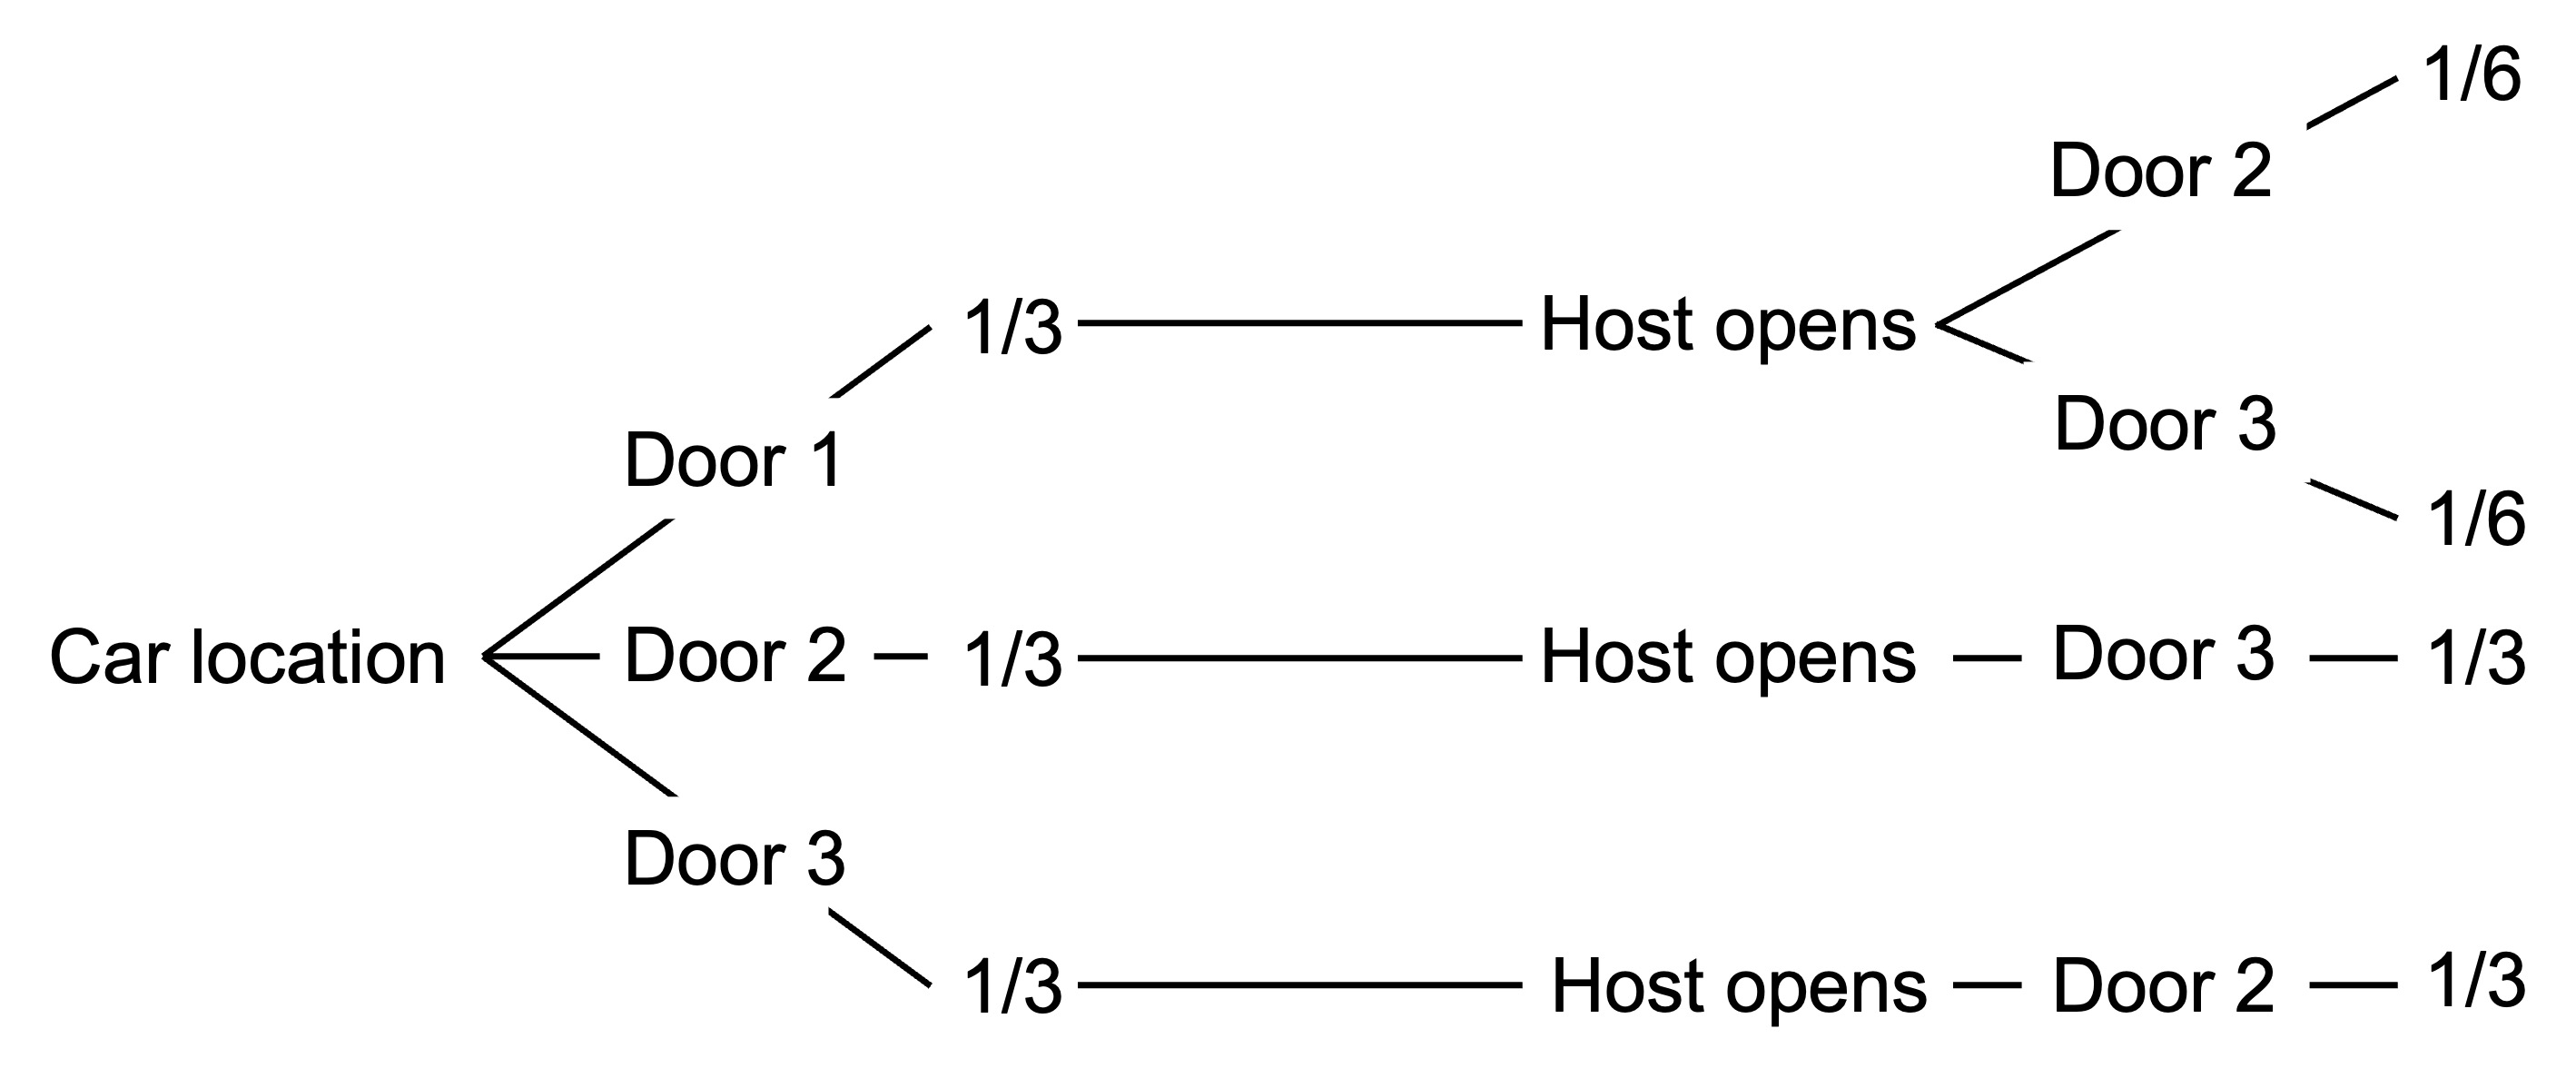
\includegraphics{beliefs/img/monty-hall.jpg}

Given the host opened Door 3:

\begin{align*}
P(C2|D3)&=\frac{P(C2\cap D3)}{P(D3)} \\[12pt]
&=\frac{\frac{1}{3}}{\frac{1}{3}+\frac{1}{6}} \\[12pt]
&=\frac{2}{3}
\end{align*}

\hypertarget{bayes-rule}{%
\section{Bayes' rule}\label{bayes-rule}}

Bayes' Rule enables estimation of the conditional probability of outcome
\(A\) given outcome \(B\) when you have the following information:

\begin{itemize}
\tightlist
\item
  The unconditional probability of outcome \(A\)
\item
  The probability of observing outcome \(B\) given outcome \(A\)
\item
  The total probability of outcome \(B\).
\end{itemize}

Bayes' rule is calculated as follows:

\begin{align*}
P(A|B)&=\frac{P(A\cap B)}{P(B)} \\[12pt]
&=\frac{P(B|A)P(A)}{P(B)}
\end{align*}

The denominator is the total probability of event \(B\). If we do not
have it directly available, we are often able to construct it with
available information concerning the conditional probabilities of \(B\)
given the occurrence (or not) of \(A\).

\[
P(B)=P(B|A)P(A)+P(B|\neg A)P(\neg A)
\]

The symbol \(\neg\) represents ``not''.

We can therefore write Bayes' rule as follows:

\begin{align*}
P(A|B)&=\frac{P(B|A)P(A)}{P(B)} \\[12pt]
&=\frac{P(B|A)P(A)}{P(B|A)P(A)+P(B|\neg A)P(\neg A)}
\end{align*}

We can also think of Bayes' rule as how we should update our belief
\(H\) (``hypothesis'') in the light of a new event \(E\).

Rational agents should update their belief \(H\) using Bayes' rule.

In this case we have the following elements:

\begin{itemize}
\item
  A belief \(H\) (often called the posterior belief)
\item
  The prior probability \(P(H)\) of \(H\)𝐻 being true
\item
  The probability \(P(E|H)\) of observing event \(E\) given a belief
\item
  The posterior probability \(P(H|E)\) of the belief given the event
  \(E\)
\end{itemize}

Under this framing, Bayes' rule is formulated as follows:

\begin{align*}
\underbrace{P(H|E)}_\text{Posterior belief}&=\frac{P(E|H)\overbrace{P(H)}^\text{Prior belief}}{P(E)} \\[12pt]
&=\frac{P(E|H)P(H)}{P(E|H)P(H)+P(E|\neg H)P(\neg H)}
\end{align*}

\hypertarget{bayes-rule-example-1}{%
\subsection{Bayes' rule example 1}\label{bayes-rule-example-1}}

Suppose your friend has two coins. One is a fair coin with a head on one
face and a tail on the other. The second coin is a rigged coin with
heads on both faces.

Your friend then takes one of the coins and flips it. It shows a head.
What is the probability that it is the rigged coin?

We will assume that he randomly selected either coin with probability
50\%. We take that as our prior belief:

\[
P(\text{rigged})=0.5
\]

The probability of a head if it is the rigged coin is 1.

\[
P(\text{head}|\text{rigged})=1
\]

To use Bayes' rule we need the total probability that a head comes up,
\(P(\text{head})\).

Here we will use the formula for total probability that we looked at
previously.

\begin{align*}
P(\text{head})&=P(\text{head}|\text{rigged})P(\text{rigged})+P(\text{head}|\text{fair})P(\text{fair}) \\
&=1\times 0.5+0.5\times 0.5 \\
&=0.75
\end{align*}

Putting this into Bayes rule:

\begin{align*}
P(\text{rigged}|\text{head})&=\frac{P(\text{head}|\text{rigged})P(\text{rigged})}{P(\text{head})} \\[12pt]
&=\frac{1\times 0.5}{0.75} \\
&=\frac{2}{3}
\end{align*}

Your friend flips the coin again and gets another head. What is the
updated probability that the coin is rigged?

\begin{align*}
P(\text{rigged}|\text{head})&=\frac{P(\text{head}|\text{rigged})P(\text{rigged})}{P(\text{head}|\text{rigged})P(\text{rigged})+P(\text{head}|\text{fair})P(\text{fair})} \\[12pt]
&=\frac{1\times \frac{2}{3}}{1\times\frac{2}{3}+\frac{1}{2}\times\frac{1}{3}} \\
&=\frac{4}{5}
\end{align*}

Your friend flips the coin 10 more times and gets 10 more heads. What is
the updated probability that the coin is rigged?

\begin{align*}
P(\text{rigged}|\text{10 heads})&=\frac{P(\text{10 heads}|\text{rigged})P(\text{rigged})}{P(\text{10 heads}|\text{rigged})P(\text{rigged})+P(\text{10 heads}|\text{fair})P(\text{fair})} \\[12pt]
&=\frac{1\times \frac{4}{5}}{1\times\frac{4}{5}+(\frac{1}{2})^{10}\times\frac{1}{5}} \\[6pt]
&=\frac{1\times \frac{4}{5}}{1\times\frac{4}{5}+\frac{1}{1024}\times\frac{1}{5}} \\[6pt]
&=0.9997559
\end{align*}

\hypertarget{bayes-rule-example-2}{%
\subsection{Bayes' rule example 2}\label{bayes-rule-example-2}}

You have two urns. Urn one has 30\% black balls and 70\% yellow balls.
Urn two has 70\% black balls and 30\% yellow balls. The labels have
fallen off the urns so you do not know which urn is which.

You reach into one of the urns and pull out a yellow ball. What is the
probability that you have drawn the ball from urn one?

\begin{align*}
P(\text{urn one}|\text{yellow ball})&=\frac{P(\text{yellow ball}|\text{urn one})P(\text{urn one})}{P(\text{yellow ball})} \\[6pt]
&=\frac{P(\text{yellow ball}|\text{urn one})P(\text{urn one})}{P(\text{yellow ball}|\text{urn one})P(\text{urn one})+P(\text{yellow ball}|\text{urn two})P(\text{urn two})} \\[6pt]
&=\frac{0.7\times 0.5}{0.7\times 0.5+0.3\times 0.5} \\[6pt]
&=\frac{0.35}{0.5} \\
&=0.7
\end{align*}

You put the first ball back in the urn, reach in again and pull out a
black ball. What is the probability that you have drawn the ball from
urn one?

\begin{align*}
P(\text{urn one}|\text{black ball})&=\frac{P(\text{black ball}|\text{urn one})P(\text{urn one})}{P(\text{black ball})} \\[6pt]
&=\frac{P(\text{black ball}|\text{urn one})P(\text{urn one})}{P(\text{black ball}|\text{urn one})P(\text{urn one})+P(\text{black ball}|\text{urn two})P(\text{urn two})} \\[6pt]
&=\frac{0.3\times 0.7}{0.3\times 0.7+0.7\times 0.3} \\[6pt]
&=\frac{0.21}{0.42} \\
&=0.5
\end{align*}

\hypertarget{bayes-rule-example-3}{%
\subsection{Bayes' rule example 3}\label{bayes-rule-example-3}}

Recall the Monty Hall problem:

\begin{quote}
Suppose you're on a game show and you're given the choice of three
doors: Behind one door is a car; behind the others, goats. You pick a
door, say No.~1, and the host, who knows what's behind the doors, opens
another door, say No.~3, which has a goat. He then says to you, ``Do you
want to pick door No.~2?'' Is it to your advantage to switch your
choice?
\end{quote}

Assume that the rules of this game show are that:

\begin{itemize}
\item
  The host must always open a door that you did not choose.
\item
  The host must always open a door to reveal a goat and never the car.
\item
  The host must always offer you the choice to switch between the chosen
  door and the remaining closed door.
\end{itemize}

We want to know the probability that the car is behind door 2 given the
host opened door 3. That is, we want to know \(P(C2|D3)\).
{[}Technically we want \(P(C2|D3\cap X1)\) where X1 is our selection of
door 1. However, adding this complication to the calculation does not
change the answer.{]}

To determine this using Bayes rule, we would use the following formula:

\begin{align*}
P(A|B)&=\frac{P(B|A)P(A)}{P(B)} \\[12pt]
P(C2|D3)&=\frac{P(D3|C2)P(C2)}{P(D3)} \\[12pt]
&=\frac{P(D3|C2)P(C2)}{P(D3|C2)P(C2)+P(D3|C1)P(C1)+P(D3|C3)P(C3)} \\[12pt]
&=\frac{1\times\frac{1}{3}}{1\times\frac{1}{3}+\frac{1}{2}\times\frac{1}{3}+0\times\frac{1}{3}} \\[12pt]
&=\frac{\frac{1}{3}}{\frac{1}{2}} \\[12pt]
&=\frac{2}{3}
\end{align*}

\hypertarget{heuristics}{%
\chapter{Heuristics}\label{heuristics}}

Heuristics are mental shortcuts or rules of thumb that people use to
make decisions. They differ from optimisation in that they often use a
limited set of information and a more computationally tractable method
for making a satisfactory decision.

There is substantial evidence that people use heuristics. They don't
normally calculate conditional probabilities using Bayes rule. Rather,
the heuristics approximate Bayes rule under certain conditions.

Heuristics are often accurate, are tractable, but in certain
environments can lead to error.

Tversky and Kahneman (1974) defined three now classic heuristics:
representativeness, availability and anchoring.

I will illustrate these three and then discuss a series of biases in
probability judgment for which these heuristics may provide an
explanation.

\hypertarget{representativeness-heuristic}{%
\section{Representativeness
heuristic}\label{representativeness-heuristic}}

Suppose you wish to estimate the probability that an event or person
belongs to a certain class.

\begin{itemize}
\item
  ``What is the probability that the event \(A\) belongs to the class
  \(B\)?''
\item
  ``What is the probability that the process \(B\) will generate the
  event \(A\)?''
\end{itemize}

Under the representativeness heuristic, probabilities are evaluated by
the degree to which \(A\) is representative of (similar to) \(B\).

Tversky and Kahneman (1974) provide the following example:

\begin{quote}
For an illustration of judgment by representativeness, consider an
individual who has been described by a former neighbor as follows:

``Steve is very shy and withdrawn, invariably helpful, but with little
interest in people, or in the world of reality. A meek and tidy soul, he
has a need for order and structure, and a passion for detail.''

How do people assess the probability that Steve is engaged in a
particular occupation from a list of possibilities (for example, farmer,
salesman, airline pilot, librarian, or physician)? How do people order
these occupations from most to least likely? In the representativeness
heuristic, the probability that Steve is a Iibrarian, for example, is
assessed by the degree to which he is representative of, or similar to,
the stereotype of a librarian. Indeed, research with problems of this
type has shown that people order the occupations by probability and by
similarity in exactly the same way.
\end{quote}

\hypertarget{availability-heuristic}{%
\section{Availability heuristic}\label{availability-heuristic}}

Under the availability heuristic, people assess the frequency of a class
or the probability of an event by the ease with which instances or
occurrences can be recalled. If an event is more ``available'' it is
judged to have a higher frequency or probability.

For example, if trying to assess the probability of heart attack, you
might recall occurrences among people you know. If trying to assess the
probability of shark attack, you might recall how often you hear of
attacks on the news.

In one experiment (Tversky and Kahneman, 1974), experimental subjects
were given lists of names. In some lists the men were more famous than
the women, and in other lists vice versa. After viewing the list they
were then asked whether the list had more men or women.

For each list, the subjects judged that the sex that had more famous
names was more common. Those names were more available in their minds.

\hypertarget{anchoring-and-adjustment}{%
\section{Anchoring and adjustment}\label{anchoring-and-adjustment}}

When using the anchoring and adjustment, people estimate by starting
from an initial value and adjusting from that value to obtain the final
estimate. Suppose you know the odds of a phenomenon \(A\) and you want
to estimate the odds of phenomenon \(B\). Anchoring and adjustment
implies that:

The accuracy of anchoring and adjustment is dependent on:

\begin{enumerate}
\def\labelenumi{\arabic{enumi}.}
\item
  The quality of the anchor: Is the anchor correlated with the quantity
  being estimated? How strongly? Empirically, people tend to use weak or
  irrelevant anchors.
\item
  The size of the adjustment from the anchor. Empirically, observed
  adjustments from the anchor are too small.
\end{enumerate}

Tversky and Kahneman (1974) asked subjects to estimate the percentage of
African countries in the United Nations.

A number between 0 and 100 was determined by spinning a wheel in the
subjects' presence. The subjects were instructed to indicate first
whether that number was higher or lower than the estimated percentage,
and then to estimate the value of the quantity by moving upward or
downward from the given number.

Different groups were given different numbers from the wheel, and these
arbitrary numbers had a marked effect on estimates. The median estimates
of the percentage of African countries in the United Nations were 25 and
45 for groups that received 10 and 65, respectively.

Payoffs for accuracy did not reduce the effect of the anchor.

\hypertarget{biases-in-probability-judgment}{%
\chapter{Biases in probability
judgment}\label{biases-in-probability-judgment}}

\hypertarget{the-conjunction-fallacy}{%
\section{The conjunction fallacy}\label{the-conjunction-fallacy}}

Tversky and Kahneman (1983) asked students to read the following
statement:

\begin{quote}
Linda is 31 years old, single, outspoken, and very bright. She majored
in philosophy. As a student, she was deeply concerned with issues of
discrimination and social justice, and also participated in anti-nuclear
demonstrations.
\end{quote}

The students were asked to rank the following statements from most (1)
to least (8) probable:

\begin{enumerate}
\def\labelenumi{\arabic{enumi}.}
\tightlist
\item
  Linda is a teacher in elementary school.
\item
  Linda works in a bookstore and takes Yoga classes.
\item
  Linda is active in the feminist movement.
\item
  Linda is a psychiatric social worker.
\item
  Linda is a member of the League of Women Voters.
\item
  Linda is a bank teller.
\item
  Linda is an insurance salesperson.
\item
  Linda is a bank teller and is active in the feminist movement.
\end{enumerate}

Note that ``8. Linda is a bank teller and is active in the feminist
movement'' is a conjunction of ``3. Linda is active in the feminist
movement'' and ``6. Linda is a bank teller''.

Tversky and Kahneman found in a sample of students that 88\% had 3
before 8 before 6. ``6. Linda is a bank teller'' was rated less probable
than ``8. Linda is a bank teller and is active in the feminist
movement''.

To understand why this is an error, recall that the probability of the
conjunction of two outcomes equals:

\[
P(A\cap B)=P(A|B)P(B)=P(B|A)P(A)
\]

As \(P(A|B)\leq 1\) and \(P(B|A)\leq 1\), \(P(A\cap B)\) must be less
than or equal to \(P(A)\) or \(P(B)\). If \(P(A|B)<1\) and \(P(B|A)<1\),
\(P(A\cap B)\) must be less than \(P(A)\) or \(P(B)\).

Why do people make this error?

The description of Linda was constructed to be representative of a
feminist and unrepresentative of a bank teller.

If people used the representativeness heuristic to order the statements,
they would likely rank 8 above 6.

The Linda Problem is one of the most heavily debated experiments in the
social sciences.

For example, Hertwig and Gigerenzer (1999) argue that people infer
nonmathematical meaning to the word ``probability'', taking it to mean
``plausible'' or ``credible''.

While possibly a fair critique of the Linda problem, other illustrations
of the conjunction fallacy appear more robust.

From Tversky and Kahneman (1983):

\begin{quote}
Consider a regular six-sided die with four green faces and two red
faces. The die will be rolled 20 times and the sequence of greens (G)
and reds (R) will be recorded. You are asked to select one sequence,
from a set of three, and you will win \$25 if the sequence you chose
appears on successive rolls of the die. Please check the sequence of
greens and reds on which you prefer to bet.

\begin{enumerate}
\def\labelenumi{\arabic{enumi}.}
\item
  RGRRR
\item
  GRGRRR
\item
  GRRRRR
\end{enumerate}
\end{quote}

65\% of experimental subjects chose sequence 2. It appears more
``representative'' of a die with four green faces and two red faces. But
note that 1 is contained within 2 and strictly more likely. The fact
subjects are betting on the outcome should remove questions about
interpretation.

\hypertarget{base-rate-neglect}{%
\section{Base rate neglect}\label{base-rate-neglect}}

\hypertarget{the-cab-problem}{%
\subsection{The cab problem}\label{the-cab-problem}}

The cab problem from Tversky and Kahneman (1982) involves the following
story:

\begin{quote}
A cab was involved in a hit and run accident at night. Two cab
companies, the Green and the Blue, operate in the city. Participants are
given the following data:

\begin{enumerate}
\def\labelenumi{\arabic{enumi}.}
\item
  85\% of the cabs in the city are Green, 15\% are Blue
\item
  A witness identified the cab as Blue. The court tested the reliability
  of the witness under the same circumstances that existed on the night
  of the accident and concluded that the witness correctly identified
  each one of the two colours 80\% of the time.
\end{enumerate}

What is the probability that the cab involved in the accident was Blue
rather than Green?
\end{quote}

In the experiment, the median and modal answer was 80\%.

The correct answer is 41\%.

The experimental result indicates a confusion between conditional
probabilities.

\[
\underbrace{P(\text{claim blue}|\text{blue})}_{80\%}\neq \underbrace{P(\text{blue}|\text{claim blue})}_{\text{Requires Bayes' rule}}
\]

The experimental subjects were effectively neglecting the base rate (the
relative rarity) of blue cabs. A witness seeing a blue cab is
representative of what would occur if the cab were blue.

The correct answer is as follows:

\begin{align*}
P(\text{blue}|\text{claim blue})&=\frac{P(\text{claim blue}|\text{blue})P(\text{blue})}{P(\text{claim blue}|\text{blue})P(\text{blue})+P(\text{claim blue}|\neg\text{blue})P(\neg\text{blue})} \\[12pt]
&=\frac{0.8\times 0.15}{0.8\times 0.1+0.2\times 0.85} \\[12pt]
&=0.41
\end{align*}

\hypertarget{medical-diagnosis}{%
\subsection{Medical diagnosis}\label{medical-diagnosis}}

Consider the following problem:

\begin{quote}
You test yourself for COVID-19. The following information is known:

\begin{itemize}
\item
  The probability that a person has COVID-19 is 1\% (the prevalence)
\item
  If a person has COVID-19, the probability that they test~positive is
  90\% (the sensitivity)
\item
  If a person does not have COVID-19, the probability that
  they~nevertheless test~positive is 9\% (the false positive rate).
\end{itemize}

You test positive. What is the chance that you have COVID-19?
\end{quote}

When problems of this nature are given to physicians, only around 10 to
20\% reason according to Bayes' rule (for example, see Hoffrage et al.
(2015)).

The most common answers approximate the sensitivity (\textasciitilde90\%
for this example).

As for the cab problem, there is a confusion about sensitivity.

\[
P(\text{COVID}|\text{positive})\neq P(\text{positive}|\text{COVID})
\]

A positive test is ``representative'' of someone with COVID-19, so is
given greater weight than the more general information about the base
rate.

The correct answer is:

\begin{align*}
P(\text{COVID}|\text{positive})&=\frac{P(\text{positive}|\text{COVID})P(\text{COVID})}{P(\text{positive})} \\[12pt]
&=\frac{P(\text{positive}|\text{COVID})P(\text{COVID})}{P(\text{positive}|\text{COVID})P(\text{COVID})+P(\text{positive}|\neg\text{COVID})P(\neg\text{COVID})} \\[12pt]
&=\frac{0.9\times 0.01}{0.9\times 0.01 + 0.09\times 0.99} \\[12pt]
&=0.092
\end{align*}

The correct answer becomes more apparent if I show an alternative
representation, such as the following:

\begin{quote}
You test yourself with a rapid antigen test for COVID-19. The following
information is known:

\begin{itemize}
\tightlist
\item
  Ten in every 1000 people have COVID-19~(the prevalence)
\item
  Of these 10 people with COVID-19, nine will test positive (the
  sensitivity)
\item
  Of the 990 people without COVID-19, about 89 nevertheless test
  positive (the false positive rate).
\end{itemize}

You test positive. What is the chance that you have COVID-19?
\end{quote}

Use of natural frequencies in this way was first proposed by Cosmides
and Tooby (1996). Natural frequencies are derived from observing cases
that have been representatively sampled from a population.

Hoffrage and Gigerenzer (1998) report that this change in representation
increased the proportion of correct answers among physicians from 10\%
to 46\%.

There is some evidence that you can get further gains through a
frequency tree representation (e.g. Spiegelhalter and Gage (2015)).
Below is one such tree from Gigerenzer (2011).

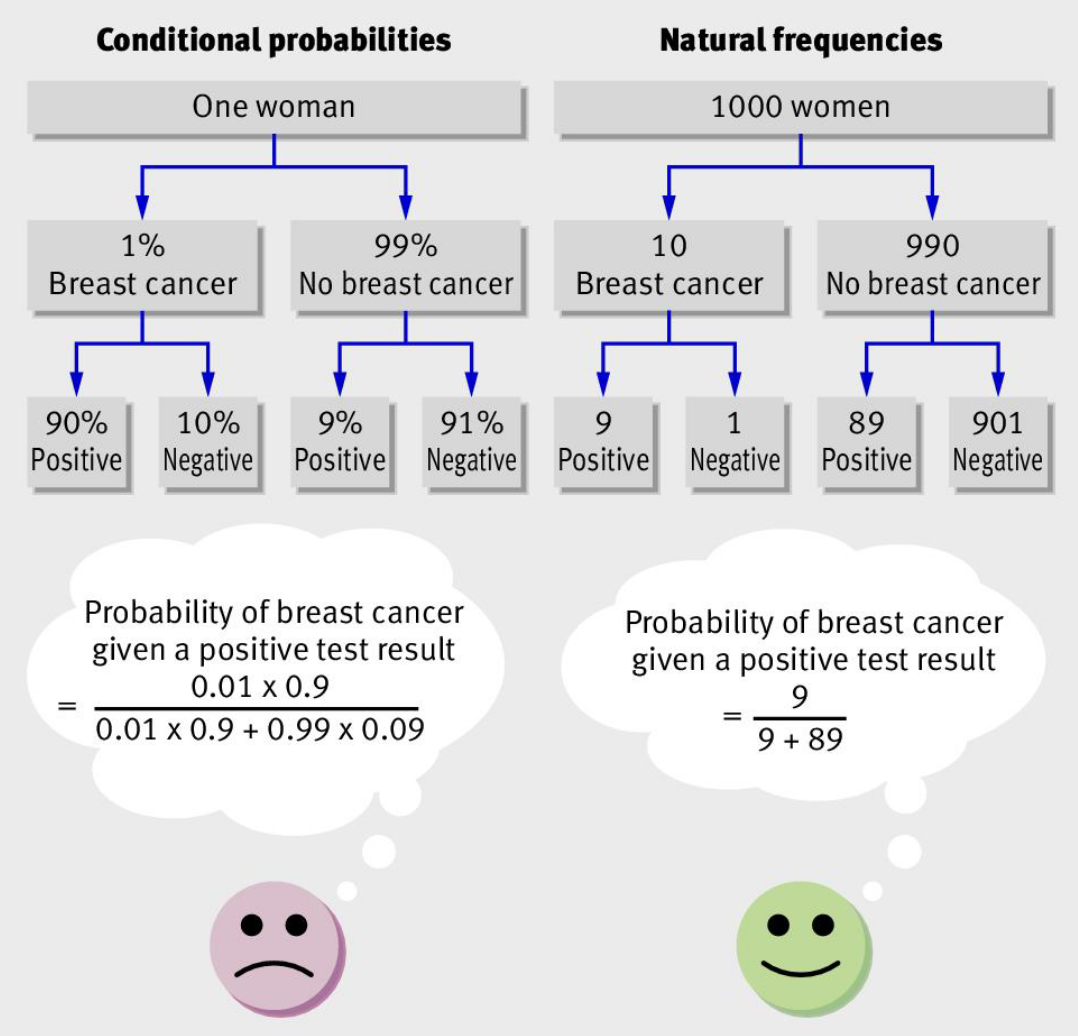
\includegraphics{beliefs/img/gigerenzer_2011.png}

The numbers at the bottom of the conditional probability tree do not
contain the base rate information. You can't simply compare across them
in calculating conditional probabilities. You also need to refer back to
the middle layer. Conversely, the natural frequency tree contains all
you need in the bottom row.

Note that we could convert the numbers in the bottom of the conditional
probability tree into frequencies: 900 in 1000, 10 in 1000, 90 in 1000
and 910 in 1000. Gigerenzer calls these simple frequencies.

There are many scenarios where simple frequencies can make a problem
more tractable, but they do not solve the computational complexity here.
Simple frequencies are just a restatement of the probabilities. In
contrast, natural frequencies are joint frequencies, such as the number
of people who test positive and who have COVID-19.

\hypertarget{the-quasi-bayesian-approach}{%
\subsection{The Quasi-Bayesian
approach}\label{the-quasi-bayesian-approach}}

We can introduce base-rate neglect into Bayes' formula by assuming
people put the same probability on all possible hypotheses (uniform
priors).

For example, base-rate neglect implies we assume the COVID-19 and
non-COVID-19 population have the same size. The two possible states of
the world (COVID-19+, COVID-19−) are assumed to have the same
probability (\(p=0.5\), \(1−p=0.5\)).

By introducing the base-rate neglect in Bayes' rule we match the
empirical result:

\begin{align*}
P(\text{COVID}|\text{positive})&=\frac{P(\text{positive}|\text{COVID})P(\text{COVID})}{P(\text{positive})} \\[12pt]
&=\frac{P(\text{positive}|\text{COVID})P(\text{COVID})}{P(\text{positive}|\text{COVID})P(\text{COVID})+P(\text{positive}|\neg\text{COVID})P(\neg\text{COVID})} \\[12pt]
&=\frac{0.9\times 0.5}{0.9\times 0.5 + 0.09\times 0.5} \\[12pt]
&=0.909
\end{align*}

\hypertarget{probability-matching}{%
\section{Probability matching}\label{probability-matching}}

Consider the following experimental setup:

\begin{itemize}
\tightlist
\item
  A red lamp that turns on with probability \(p=0.70\)
\item
  A green lamp that turns on with probability \(p=0.30\)
\end{itemize}

Participants are required top predict which light will turn on after
observing a series of flashes.

What do participants do?

The proportions of predictions reflect the actual probabilities of the
two light bulbs being turned on (i.e.~\(p=0.30\) for green lamps,
\(p=0.70\) for red lamps)

Probability matching is the tendency of humans and animals to mirror the
probability distributions of presented stimuli in their response
probabilities. The strategy of probability matching is not optimal for
minimizing prediction error.

With probability matching, the probability of a successful guess is:

\begin{align*}
P(\text{success})&=0.7\times 0.7+0.3\times0.3 \\
&=0.58
\end{align*}

A better strategy is to always select the event with the highest
probability. In this example, participants should always predict that
the red light will be turned on, giving them a 70\% probability of a
successful guess.

\hypertarget{the-gamblers-fallacy}{%
\section{The gambler's fallacy}\label{the-gamblers-fallacy}}

The gambler's fallacy is the false belief that in a sequence of
independent draws from a distribution an outcome that has not realized
for a while is more likely to occur on the next draw.

For example, following three flips of a coin that all come up heads, a
person experiencing the gambler's fallacy would believe that a tail is
more likely on the next flip.

Using data from Rapoport and Budescu (1997), Rabin and Vayanos (2010)
derived the probability with which the next flip of a coin will be heads
given the last three flips being heads or tails.

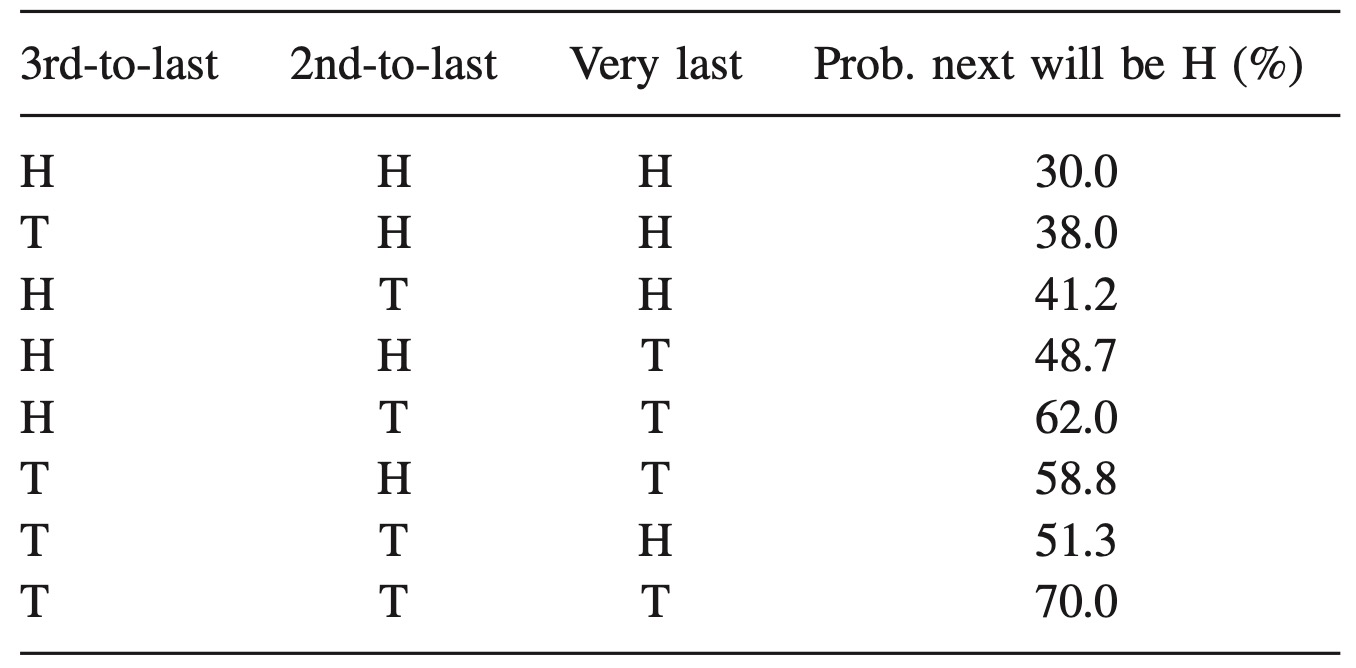
\includegraphics{beliefs/img/gamblers-fallacy.jpg}

One explanation for the gambler's fallacy is representativeness. For
example, the sequence of coin flips HHHHHH is not seen as representative
of flipping a fair coin six times. HHTTHH is seen as more
representative.

An alternative explanation is that people believe in the ``law of small
numbers''. They overestimate the degree to which a small sample will
resemble the population from which it is drawn. For example, if a fair
coin is flipped six times, they will overestimate the likelihood the
result will be three heads and three tails.

\hypertarget{the-law-of-small-numbers}{%
\subsection{The law of small numbers}\label{the-law-of-small-numbers}}

The following model of the law of small numbers comes from Rabin (2002).

Imagine an urn filled with red balls and black balls. You draw balls
from the urn with replacement. The red balls are drawn with probability
\(p\) and the black balls are drawn with probability \(1−p\).

Assume Freddy knows the probabilities \(p\) and \(1−p\) but (wrongly)
assumes balls are drawn from the urn without replacement. That is, the
outcomes are subject to the law of small numbers. If he assumes there
are \(N\) balls in the urn, he expects a sample of \(N\) balls to match
\(p\) and \(1−p\).

For small \(N\), each draw from the urn without replacement is
informative about future draws. For large \(N\), a single draw without
replacement does not materially affect the probability of the next ball.

Under Freddy's beliefs, outcomes must be correlated, rather than the
true process where balls are replaced and the outcomes are uncorrelated.

Imagine Freddy plays roulette. The roulette wheel contains 36 slots, 18
black and 18 red.

Freddy observes 4 spins of the wheel before betting. He observes the
sequence RRRR.

We assume a bias of \(N=36\). Given \(p=0.5\), this implies 18 red, 18
black balls in the urn.

An unbiased belief would be that the sequence of reds tells them nothing
about future draws because the outcomes are uncorrelated.

Freddy's belief is that, after four reds, black is more likely on next
spin.

Freddy is suffering from the Gambler's Fallacy. He's wrongly computing:

\begin{align*}
\hat P(R)&=\frac{\text{total reds}}{\text{total reds}+\text{total blacks}} \\
&=\frac{18}{18+18} \\
&=0.5 \\
\hat P(RR|R)&=\frac{18-1}{(18-1)+18} \\
&=0.486 \\
\hat P(RRR|RR)&=\frac{18-2}{(18-2)+18} \\
&=0.471 \\
\hat P(RRRR|RRR)&=\frac{18-3}{(18-3)+18} \\
&=0.455
\end{align*}

In reality \(P(RR|R)=P(RRR|RR)=P(RRRR|RRR)=0.5\).

\hypertarget{hot-hand-fallacy}{%
\section{Hot hand fallacy}\label{hot-hand-fallacy}}

A person subject to the hot hand fallacy believes a streak will persist
despite the process being random and each outcome being independent of
the last.

For example:

\begin{enumerate}
\def\labelenumi{\arabic{enumi}.}
\tightlist
\item
  Commentators observe player performing a series of shots during a
  game.
\item
  The commentators compound the series of shots into a single judgment
  (the streak).
\item
  The commentators make predictions based upon the observed streak:
  ``The player has a hot hand''.
\item
  Good shots are considered more likely conditional on observing the
  streak.
\end{enumerate}

An example comes from Gilovich et al. (1985).

Imagine a person who took ten shots in a basketball game. A ball is a
hit, an X is a miss.

What would count as evidence of a hot hand? What we can do is look at
shots following a previous hit. For instance, in this sequence of shots
there are 6 occasions where we have a shot following a previous hit.
Five of those shots, such as the seventh here, are followed by another
hit.


\includegraphics{beliefs/img/hot-hand.jpg}

We can then compare their normal shooting percentage with the proportion
of shots they hit if the shot immediately before was a hit. If their hit
rate after a hit is higher than their normal shot probability, then we
might say they get a hot hand.

Using this methodology, Gilovich et al TO ADD took shot data from a
variety of sources, including the Philadelphia 76ers and Boston Celtics,
and examined it for evidence of a hot hand. They also looked at whether
there was a hit or miss after longer streaks of hits or misses.

From this data, they argued that the hot hand was an illusion.

The existence of the hot hand is disputed (e.g. Bar-Eli et al. (2006)).

\hypertarget{a-bias-in-sequences}{%
\subsection{A bias in sequences}\label{a-bias-in-sequences}}

Miller and Sanjurjo (2018) provide the most compelling critique. They
found a statistical bias in the analysis by Gilovich et al.~Correcting
for the bias they found that the probability of hitting a shot following
a sequence of three previous hits is 13 percentage points higher than
after a sequence of three misses.

The intuition behind Miller and Sanjurjo (2018) is as follows.

Suppose you flip a coin three times. There are eight possible sequences
of heads and tails. Each sequence has an equal probability of occurring.

What if I asked you: if you were to flip a coin three times, and there
is a heads followed by another flip in that sequence, what is the
expected probability that another heads will follow that heads?

In Table~\ref{tbl-hothand} below is the proportion of heads following a
previous flip of heads for each sequence. In the first row of the table,
the first flip is a head. That first flip is followed by another head.
After the second flip, a head, we also have a head. There is no flip
after the third head. 100\% of the heads in that sequence followed by
another flip are followed by a head.

In the second row of the table, 50\% of the heads are followed by a
head. In the last two rows, there are no heads followed by another flip.

Now, back to our question: if you were to flip a coin three times, and
there is a heads followed by another flip in that sequence, what is the
expected probability that another heads will follow that heads? It turns
out it is 42\%, which I can get by averaging those proportions.

\hypertarget{tbl-hothand}{}
\begin{longtable}[]{@{}ll@{}}
\caption{\label{tbl-hothand}Eight possible combinations of heads and
tales across three flips}\tabularnewline
\toprule()
Flips & \(p(H_{t+1}|H_t)\) \\
\midrule()
\endfirsthead
\toprule()
Flips & \(p(H_{t+1}|H_t)\) \\
\midrule()
\endhead
HHH & 100\% \\
HHT & 50\% \\
HTH & 0\% \\
HTT & 0\% \\
THH & 100\% \\
THT & 0\% \\
TTH & - \\
TTT & - \\
\textbf{Expected value} & \textbf{42\%} \\
\bottomrule()
\end{longtable}

That contrasts with what we get we count across all the sequences, where
we see that there are 8 flips of heads that are followed by another
flip. Of the subsequent flips, 4 are heads and 4 are tails, which is the
50\% you expect.

Why that difference? By looking at these short sequences, we are
introducing a bias. The cases of heads following heads tend to cluster
together, such as in the first sequence which has two cases of a heads
following a heads. Yet the sequence THT, which has only one shot
occurring after a heads, is equally likely to occur as HHH. The reason a
tails appears more likely to follow a heads is because of this bias
whereby the streaks tend to cluster together. The expected value I get
when taking a series of three flips is 42\%, when in fact the actual
probability of a heads following a heads is 50\%. As the sequence of
flips gets longer, the size of the bias is reduced, although it is
increased if we examine longer streaks, such as the probability of a
heads after three previous heads.

This bias is relevant to the analysis of the hot hand as it is present
in the methodology of the papers that purportedly demonstrated that
there was no hot hand in basketball. Because of this bias, the
proportion of hits following a hit or sequence of hits is biased
downwards. Like our calculation using coins, the expected proportion of
hits following a hit in a sequence is lower than the actual probability
of hitting a shot.

Conversely the hot hand pushes the probability of hitting a shot after a
previous hit up. Together, the downward bias and the hot hand roughly
cancelled each other out, leading to the conclusion by researchers that
each shot is independent of the last.

The result is, that when you correct for the bias, there actually is a
hot hand in basketball.

\hypertarget{alternative-intuition}{%
\subsection{Alternative intuition}\label{alternative-intuition}}

Here is another intuition for why there is a bias in this sequence.

We flip three coins and select at random one of the flips that follows a
heads. This means that if we select a flip that follows a head we will
select either flip 2 or flip 3.

If we select flip 2, we know that flip 1 was a head. The first two flips
in the sequence are either HT or HH.

However, we can also say that if we select flip 2, HT is twice as likely
as HH. Why? Because if the first two coins were HH we could also have
selected flip 3.

That is, if the first two flips are HT, we can only select flip 2. We
select flip 2 with 100\% probability. If the first two flips are HH, we
select flip 2 with 50\% probability and flip 3 with 50\% probability.

The result is that we are twice as likely to observe HT as HH given we
selected flip 2.

Using Bayes' rule:

\begin{align*}
P(HT|\text{flip 2})&=\frac{P(\text{flip 2}|HT)P(HT)}{P(\text{flip 2})} \\[6pt]
&=\frac{P(\text{flip 2}|HT)P(HT)}{P(\text{flip 2}|HT)P(HT)+P(\text{flip 2}|HH)P(HH)} \\[6pt]
&=\frac{1\times 0.5}{1\times 0.5+0.5\times 0.5} \\[6pt]
=\frac{2}{3} \\[6pt]
\\
P(HH|\text{flip 2})&=\frac{P(\text{flip 2}|HH)P(HH)}{P(\text{flip 2})} \\[6pt]
&=\frac{P(\text{flip 2}|HH)P(HH)}{P(\text{flip 2}|HH)P(HH)+P(\text{flip 2}|HT)P(HT)} \\[6pt]
&=\frac{0.5\times 0.5}{0.5\times 0.5+1\times 0.5} \\[6pt]
=\frac{1}{3} \\[6pt]
\end{align*}

\hypertarget{the-hot-hand-fallacy-for-truly-random-sequences}{%
\subsection{The hot hand fallacy for truly random
sequences}\label{the-hot-hand-fallacy-for-truly-random-sequences}}

However, there is strong evidence that people see streaks in processes
that are truly random, with each outcome independent of the last. For
example, Ayton and Fisher (2004) find that when people are predicting
the results of the spins of a roulette wheel, they increase the
confidence of their predictions after a series of successes. This occurs
despite the outcome being random. (Note: they also exhibit the gambler's
fallacy in what they predict.)

\hypertarget{heuristics-and-the-bias-variance-trade-off}{%
\chapter{Heuristics and the bias-variance
trade-off}\label{heuristics-and-the-bias-variance-trade-off}}

While much of the heuristics and biases literature of Kahneman, Tversky
and those who followed in their footsteps focuses on the errors that can
be caused by the use of heuristics, there are also powerful reasons for
their use.

One of the strongest arguments for the use of simple heuristics relates
to what is called the bias-variance trade-off.

Suppose you are trying to make a prediction or develop an estimate based
on historical data. There is a true underlying process that is
generating the data. You plan to build a predictive model that should
approximate the underlying process. You have a noisy data sample with
which to develop it and you are trying to decide which predictors to
include.

An example of this could be that you want to predict the level of drop
out in a school. You have possible predictors such as attendance rates,
family socio-economic status, the school's average SAT score, and the
degree of parental involvement in the child's schooling. Which of those
should you include in your model?

Bias is the degree to which there are erroneous assumptions in your
model. The classic case of bias is when you have failed to include a
relevant predictor. If you exclude relevant predictors, you introduce
bias as your predictive model will not include relevant relations
between the predictors and the target output you are trying to predict.
On the school example above, to the extent any of these factors are
linked to drop out rates, excluding them can bias your prediction.

However, inclusion of too many predictors can lead to what is called
variance, which is an error that arises because of the sensitivity of
the model to fluctuations in the data you use to develop the model. It
ultimately involves giving too much weight to irrelevant or marginally
relevant information.

For example, if you included the school colours in your model, it may
appear to give you a better model due to noise. But as soon as you used
it to make a new prediction, it would likely backfire.

The following image gives on conception of bias and variance. An
unbiased predictor will tend to centre on the target. A low variance
predictor will tend to cluster. A low variance, low bias estimate is the
best outcome.

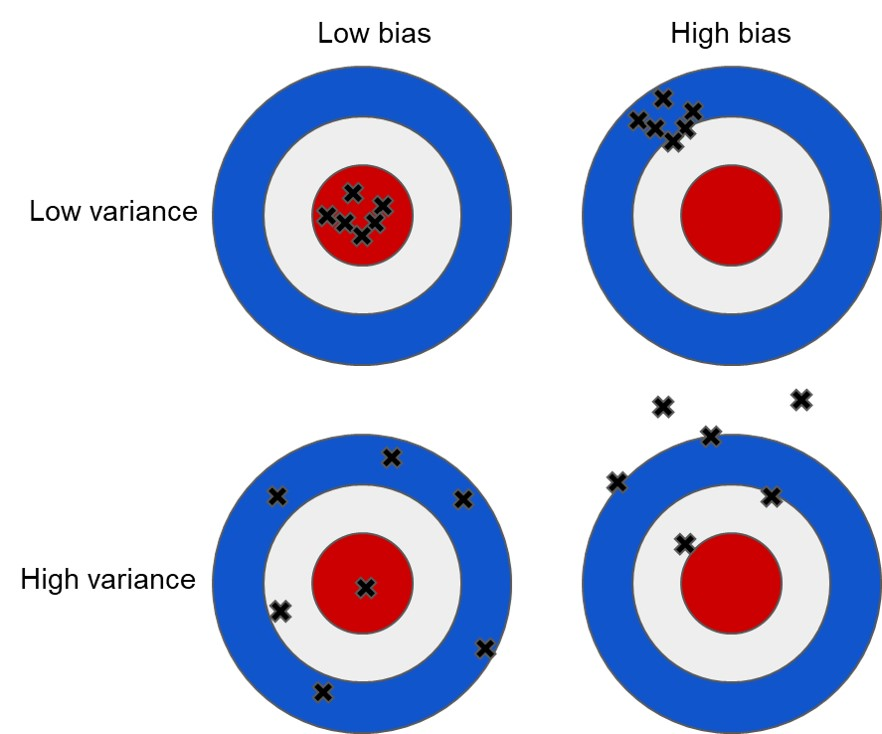
\includegraphics{beliefs/img/bias_and_variance.jpg}

However, as the term bias-variance trade-off suggests, it is not that
simple. There is a trade-off between the two. As model complexity
increases, bias tends to decrease, but variance tends to go up. There is
an optimal level of complexity.

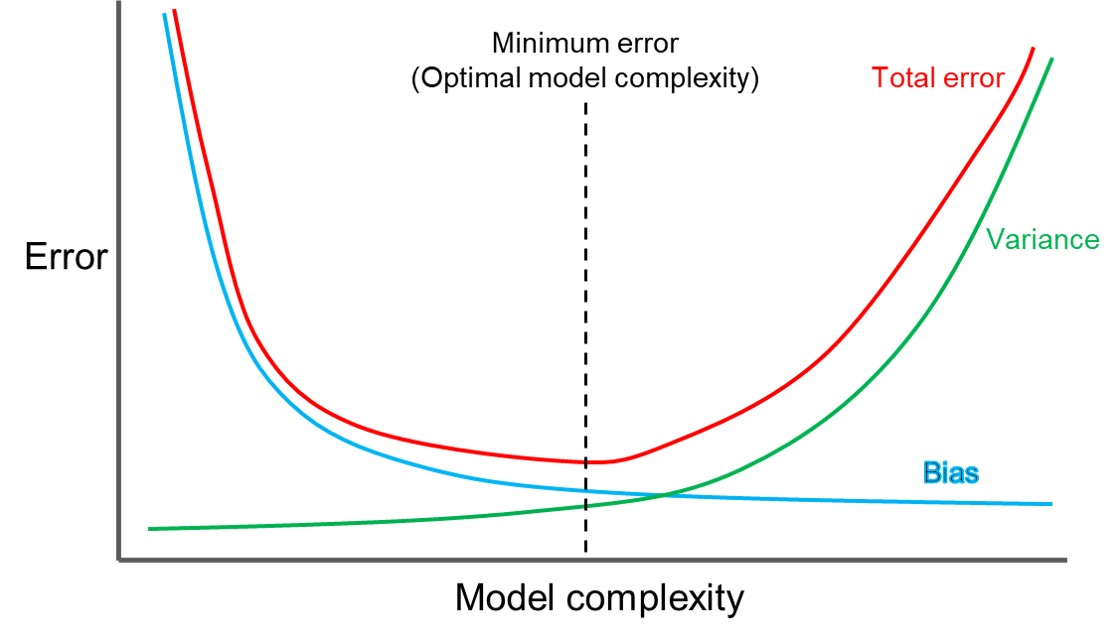
\includegraphics{beliefs/img/bias-variance_trade-off.jpg}

The result of this bias-variance trade-off means that simple heuristics
can sometimes be better than more complex decision making strategies.
This is not just because they are tractable for the human mind, but also
because they find a better bias-variance trade-off, which also leads to
better performance. Despite our focus on how heuristics can backfire in
corporate decision-making environments, there can be a power to them.

\hypertarget{example-the-gaze-heuristic}{%
\section{Example: The gaze heuristic}\label{example-the-gaze-heuristic}}

The gaze heuristic is a tool that people -- and dogs -- use to catch
balls. The heuristic is simply this -- maintain the ball at a constant
angle of gaze. If you move to keep this angle constant, you will end up
where the ball lands. Obviously, this is easier than calculating where
you should be from the velocity of the ball, angle of flight, the effect
of wind resistance and so on.

\begin{figure}

{\centering 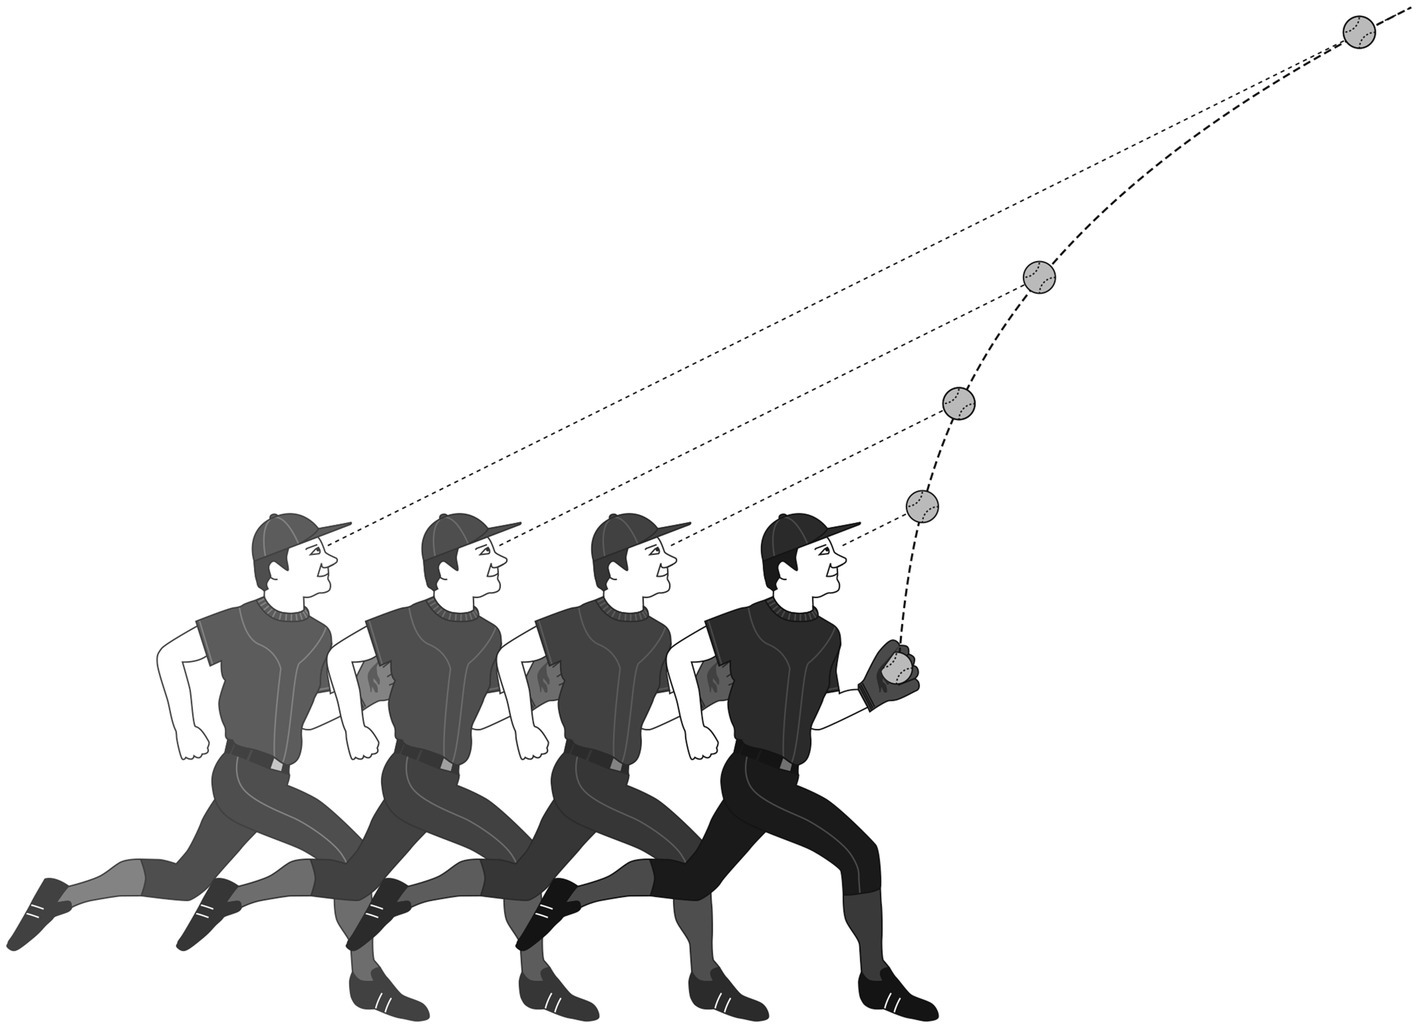
\includegraphics{beliefs/img/gaze-heuristic.jpg}

}

\caption{Source: Gigerenzer (2021)}

\end{figure}

But it results in a strange pattern of movement. Suppose you are close
to the point where the ball is first hit into the air. As it rises you
will tend to back away from the ball. As it then starts to fall, you
will move back in. If it is hit up to the side of you, you will move to
the ball in a curve. Now, if you had a behavioural economist look at the
path you took to catch the ball, they might call it the curve bias or
something like that -- but it is actually the result of a very effective
decision making tool.

There are also some circumstances where it works better, and some where
it fails. It tends to work best when the ball is already high in the
air. If you catch sight of a ball hit straight up before it has risen
far, using the heuristic for its entire flight could require first
running away from the ball and then toward it.

Understanding this is a much richer understanding than saying that the
fielder is biased because they did not run straight to where the ball
was going to land. It also points to the power of heuristics. Try to
train someone to run straight to where a ball will land and watch them
fail. Don't see heuristics as poor cousins of ``more rational''
approaches.

\hypertarget{overconfidence}{%
\chapter{Overconfidence}\label{overconfidence}}

De Bondt and Thaler (1995) wrote ``Perhaps the most robust finding in
the psychology of judgment and choice is that people are
overconfident.'' Take the following examples:

\begin{itemize}
\item
  When asked to estimate the length of the Nile by providing a range the
  respondent is 90\% sure contains the correct answer, the estimate
  typically contains the correct answer only 50\% of the time.
\item
  PGA golfers typically believe they sink around 75\% of 6 foot putts --
  some even believe they sink as many as 85\% -- when the average is
  closer to 55\%.
\item
  93\% of American drivers rate themselves as better than average. 25\%
  of high school seniors believe they are in the top 1\% in ability to
  get along with others.
\end{itemize}

There are many similar examples, all making the case that people are
generally overconfident.

But despite each being labelled as overconfidence, note that these
examples are actually three different phenomena.

\textbf{Overprecision} is the tendency to believe that our predictions
or estimates are more accurate than they actually are. The typical study
seeking to show overprecision asks for someone to give confidence ranges
for their estimates, such as estimating the length of the Nile. The
questions asking for confidence intervals above were designed to test
your precision.

\textbf{Overestimation} is the belief that we can perform at a level
beyond that which we realistically can. The evidence here is mixed. When
attempting a difficult task such as a six foot putt, we typically
overestimate. But on easy tasks, the opposite is often the case -- we
tend underestimate our performance. Whether over or underestimation
occurs depends upon the domain.

\textbf{Overplacement} is the erroneous relative judgement that we are
better than others. Obviously, we cannot all be better than average. But
this relative judgement, like overestimation, tends to vary with task
difficulty. For easy tasks, such as driving a car, we overplace and
consider ourselves better than most. But ask people where they rate for
a skill such as drawing, and most people will rate themselves as below
average. People don't suffer from pervasive overplacement. Whether they
overplace depends on what the situation is. The questions rating your
relative skill above were a test of overplacement.

You might note that we tend to both underestimate and overplace our
performance on easy tasks. We can also overestimate but underplace our
performance on difficult tasks.

So are we both underconfident and overconfident at the same time? The
blanket term of overconfidence does little justice to what is actually
occurring.

The conflation of these different effects under the umbrella of
overconfidence often plays out in stories of how overconfidence (rarely
assessed before the fact) led to someone's fall. For instance, evidence
that people tend to believe they are better drivers than average
(overplacement) is not evidence that overconfidence led someone to
pursue a disastrous corporate merger (overestimation).

\hypertarget{firm-entry}{%
\section{Firm entry}\label{firm-entry}}

Most new businesses fail within a few years. For example, one study of
US manufacturers found over 60\% of entrants had exited within five
years and almost 80\% within 10 years.

Camerer and Lovallo (1999) ran an experiment to test whether business
failure may be due to optimism about their relative skill.

The lab experiment involved a set of markets in which market entrants
were paid a set amount according to their rank within the market. Those
ranked within the ``market capacity'' would share a payment of \$50.
Those beyond the market capacity would be penalised \$10. Accordingly,
if there are 5 entrants above market capacity, the expected payoff of
all entrants is zero. More than that and it is negative.

The rank in the market was determined by either luck, through a random
draw, or a test of skill involving logic puzzles or trivia questions
about sports or current events.

In each round of the experiment, the market capacity was announced to
the players, along with whether the payoffs in the market were based on
luck or skill. The participants were then asked to forecast the expected
number of entrants (for which they earn a payment if correct) and decide
simultaneously and without communicating whether to enter into the
market. Subjects were then told how many participants had entered.

After all of the rounds, students solved puzzles or took the trivia quiz
to determine their skill rank.

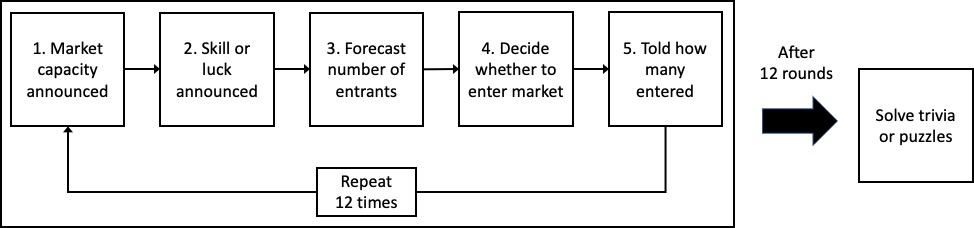
\includegraphics{beliefs/img/camerer_and_lovallo_1999.jpg}

The results of the experiment showed that more participants entered the
market when the ranking was based on skill than if based on random draw.
This indicates a belief that their skill level will rank them higher
than a random draw: they are above average.

An interesting element to this experiment was that for some of the
markets the participants were recruited by being asked if they would
like to volunteer for an experiment in which performance would depend on
their performance on sports or current event trivia questions. Hence the
pool in those markets would be stronger than typical.

In those markets with self-selected participants, market entry was even
higher, and payoffs were negative in most rounds. This suggests the
self-selected entrants were overconfident in their skill due to what
Camerer and Lovallo call ``reference group neglect''. The participants
seem to neglect that the others in the reference group also
self-selected in to the experiment and think they are skilled too.

Moore et al. (2007) ran an experiment on firm entry and found, like
Camerer and Lovallo, that entrepreneurs overweight personal factors and
underweight competitors when making entry decisions. However, when they
varied the task difficulty, they found excess entry only when the
industry appeared an easy one in which to compete. When it appeared
difficult, too few entered.

\hypertarget{trading}{%
\section{Trading}\label{trading}}

Barber and Odean (2001) write:

\begin{quote}
Theoretical models predict that overconfident investors trade
excessively. We test this prediction by partitioning investors on
gender. Psychological research demonstrates that, in areas such as
finance, men are more overconfident than women. Thus, theory predicts
that men will trade more excessively than women. Using account data for
over 35,000 households from a large discount brokerage, we analyze the
common stock investments of men and women from February 1991 through
January 1997. We document that men trade 45 percent more than women.
Trading reduces men's net returns by 2.65 percentage points a year as
opposed to 1.72 percentage points for women.
\end{quote}

The evidence they adduce in support of the gender differences is a mix
of overprecision, overplacement and overestimation.

\hypertarget{investment-decisions}{%
\section{Investment decisions}\label{investment-decisions}}

Malmendier and Tate (2005) write:

\begin{quote}
We argue that managerial overconfidence can account for corporate
investment distortions. Overconfident managers overestimate the returns
to their investment projects and view external funds as unduly costly.
Thus, they overinvest when they have abundant internal funds, but
curtail investment when they require external financing. We test the
overconfidence hypothesis, using panel data on personal portfolio and
corporate investment decisions of Forbes 500 CEOs. We classify CEOs as
overconfident if they persistently fail to reduce their personal
exposure to company-specific risk. We find that investment of
overconfident CEOs is significantly more responsive to cash flow,
particularly in equity-dependent firms.
\end{quote}

\hypertarget{probability-judgment-exercises}{%
\chapter{Probability judgment
exercises}\label{probability-judgment-exercises}}

\hypertarget{judging-a-fund-manager}{%
\section{Judging a fund manager}\label{judging-a-fund-manager}}

You want to know if a fund manager is skilled as you believe skilled
management can lead to outperformance. The following is known:

\begin{itemize}
\item
  20\% of fund managers are skilled.
\item
  If a fund manager is skilled, the probability that they outperform the
  market is 80\%.
\item
  If a fund manager is unskilled, the probability that they outperform
  the market is 40\%.
\end{itemize}

a) You observe an outperforming fund manager. What is the probability
that the fund manager is skilled?

\begin{tcolorbox}[enhanced jigsaw, title=\textcolor{quarto-callout-tip-color}{\faLightbulb}\hspace{0.5em}{Answer}, toprule=.15mm, colback=white, breakable, titlerule=0mm, colframe=quarto-callout-tip-color-frame, coltitle=black, opacityback=0, rightrule=.15mm, colbacktitle=quarto-callout-tip-color!10!white, bottomtitle=1mm, opacitybacktitle=0.6, arc=.35mm, bottomrule=.15mm, toptitle=1mm, leftrule=.75mm, left=2mm]

We calculate the solution using Bayes' rule.

\[
P(\text{skilled}|\text{outperform})=\frac{P(\text{outperform}|\text{skilled})P(\text{skilled})}{P(\text{outperform})}
\]

We can calculate \(P(outperform)\) using the law of total probability.

\begin{align*}
P(\text{outperform})&=P(\text{outperform}|\text{skilled})P(\text{skilled})+P(\text{outperform}|\text{unskilled})P(\text{unskilled}) \\[6pt]
&=0.8\times 0.2+0.4\times 0.8 \\[6pt]
&=0.48
\end{align*}

Inputting this into Bayes' rule, we get:

\begin{align*}
P(\text{skilled}|\text{outperform})&=\frac{P(\text{outperform}|\text{skilled})P(\text{skilled})}{P(\text{outperform})} \\[6pt]
&=\frac{0.8\times 0.2}{0.48} \\[6pt]
&=0.333
\end{align*}

A fund manager who outperforms is skilled with 0.333 probability. You
cannot neglect that low base rate of skilled managers.

\end{tcolorbox}

b) A person calculates the probability that the fund manager is skilled
by putting the same probability on all possible hypotheses (a uniform
prior). What do they believe is the probability that the fund manager is
skilled?

\begin{tcolorbox}[enhanced jigsaw, title=\textcolor{quarto-callout-tip-color}{\faLightbulb}\hspace{0.5em}{Answer}, toprule=.15mm, colback=white, breakable, titlerule=0mm, colframe=quarto-callout-tip-color-frame, coltitle=black, opacityback=0, rightrule=.15mm, colbacktitle=quarto-callout-tip-color!10!white, bottomtitle=1mm, opacitybacktitle=0.6, arc=.35mm, bottomrule=.15mm, toptitle=1mm, leftrule=.75mm, left=2mm]

We use Bayes' Theorem but with uniform priors.

\begin{align*}
P(\text{skilled}|\text{outperform})&=\frac{P(\text{outperform}|\text{skilled})P(\text{skilled})}{P(\text{outperform})} \\[6pt]
&=\frac{P(\text{outperform}|\text{skilled})P(\text{skilled})}{\begin{aligned}P(&\text{outperform}|\text{skilled})P(\text{skilled})\\&+P(\text{outperform}|\text{unskilled})P(\text{unskilled})\end{aligned}} \\[6pt]
&=\frac{0.8\times 0.5}{0.8\times 0.5+0.4\times 0.5} \\[6pt]
&=0.667
\end{align*}

Starting with uniform priors -- effectively ignoring the base rate --
gives us a higher probability of 67\%.

\end{tcolorbox}

\hypertarget{detecting-a-terrorist}{%
\section{Detecting a terrorist}\label{detecting-a-terrorist}}

Every month 100 million people fly on commercial airlines. Imagine 10 of
them are terrorists.

Airport security are able to correctly identify that a person is a
terrorist in 99\% of cases and a non-terrorist in 99.9\% of cases.

a) A person is identified by airport security as a terrorist. Using
Bayes' rule, what is the probability that they are a terrorist?

\begin{tcolorbox}[enhanced jigsaw, title=\textcolor{quarto-callout-tip-color}{\faLightbulb}\hspace{0.5em}{Answer}, toprule=.15mm, colback=white, breakable, titlerule=0mm, colframe=quarto-callout-tip-color-frame, coltitle=black, opacityback=0, rightrule=.15mm, colbacktitle=quarto-callout-tip-color!10!white, bottomtitle=1mm, opacitybacktitle=0.6, arc=.35mm, bottomrule=.15mm, toptitle=1mm, leftrule=.75mm, left=2mm]

We can use Bayes' Theorem to calculate the conditional probability:

\[
\begin{aligned}
P(\text{terrorist | identified}) &= \dfrac{P(\text{identified | terrorist})P(\text{terrorist})}{P(\text{identified})} \\[12 pt]
&= \dfrac{0.99*0.0000001}{0.99*0.0000001+0.001*0.999999} \\[12 pt]
&= 0.000099
\end{aligned}
\]

Or approximately 1 in 10,000.

\end{tcolorbox}

b) Intuitive responses to questions of this type tend to involve much
higher probabilities. Discuss how intuitive responses could err due to:

\begin{enumerate}
\def\labelenumi{\roman{enumi})}
\tightlist
\item
  confusion of conditional probabilities
\end{enumerate}

\begin{tcolorbox}[enhanced jigsaw, title=\textcolor{quarto-callout-tip-color}{\faLightbulb}\hspace{0.5em}{Answer}, toprule=.15mm, colback=white, breakable, titlerule=0mm, colframe=quarto-callout-tip-color-frame, coltitle=black, opacityback=0, rightrule=.15mm, colbacktitle=quarto-callout-tip-color!10!white, bottomtitle=1mm, opacitybacktitle=0.6, arc=.35mm, bottomrule=.15mm, toptitle=1mm, leftrule=.75mm, left=2mm]

If a person confuses \(P(\text{terrorist | identified})\) with
\(P(\text{identified | terrorist})\) they will wrongly assume the
probability that someone identified as a terrorist is a terrorist is
99\%. This is a common explanation for mistakes of this nature:
e.g.~identification of cabs problem discussed in class.

\end{tcolorbox}

\begin{enumerate}
\def\labelenumi{\roman{enumi})}
\setcounter{enumi}{1}
\tightlist
\item
  people placing the same probability on all possible hypotheses
  (uniform priors).
\end{enumerate}

\begin{tcolorbox}[enhanced jigsaw, title=\textcolor{quarto-callout-tip-color}{\faLightbulb}\hspace{0.5em}{Answer}, toprule=.15mm, colback=white, breakable, titlerule=0mm, colframe=quarto-callout-tip-color-frame, coltitle=black, opacityback=0, rightrule=.15mm, colbacktitle=quarto-callout-tip-color!10!white, bottomtitle=1mm, opacitybacktitle=0.6, arc=.35mm, bottomrule=.15mm, toptitle=1mm, leftrule=.75mm, left=2mm]

If a person assumed uniform priors on any individual, they would
calculate Bayes' Theorem as follows:

\[
\begin{aligned}
P(\text{terrorist | identified}) &= \dfrac{P(\text{identified | terrorist})P(\text{terrorist})}{P(\text{identified})} \\[12 pt]
&= \dfrac{0.99*0.5}{0.99*0.5+0.001*0.5} \\[12 pt]
&= 0.999
\end{aligned}
\]

This is substantially higher than the actual probability.

\end{tcolorbox}

c) State and solve the question in part a) in terms of natural
frequencies.

\begin{tcolorbox}[enhanced jigsaw, title=\textcolor{quarto-callout-tip-color}{\faLightbulb}\hspace{0.5em}{Answer}, toprule=.15mm, colback=white, breakable, titlerule=0mm, colframe=quarto-callout-tip-color-frame, coltitle=black, opacityback=0, rightrule=.15mm, colbacktitle=quarto-callout-tip-color!10!white, bottomtitle=1mm, opacitybacktitle=0.6, arc=.35mm, bottomrule=.15mm, toptitle=1mm, leftrule=.75mm, left=2mm]

Number of passengers: 100,000,000

Number of terrorists: 10

Number of terrorists identified as terrorists: 10*0.999 \(\approx\) 10

Number of non-terrorists identified as terrorists:
0.001*100,000,000=100,000

Proportion of people identified as terrorists who are terrorists =
10/(10+100000) \(\approx\) 1 in 10000

\end{tcolorbox}

\hypertarget{rolling-a-die}{%
\section{Rolling a die}\label{rolling-a-die}}

You have two six-sided dice:

\begin{itemize}
\item
  one die is fair with the numbers 1 through to 6 occurring with equal
  probability
\item
  the other die is loaded and always rolls a 5 or a 6 with equal
  probability.
\end{itemize}

You pull one die out of your pocket and roll it. You did not check which
die it was before you rolled. (Assume you could have pulled either die
out of your pocket with equal probability.)

a) The die shows a six. What is the probability that it is the loaded
die?

\begin{tcolorbox}[enhanced jigsaw, title=\textcolor{quarto-callout-tip-color}{\faLightbulb}\hspace{0.5em}{Answer}, toprule=.15mm, colback=white, breakable, titlerule=0mm, colframe=quarto-callout-tip-color-frame, coltitle=black, opacityback=0, rightrule=.15mm, colbacktitle=quarto-callout-tip-color!10!white, bottomtitle=1mm, opacitybacktitle=0.6, arc=.35mm, bottomrule=.15mm, toptitle=1mm, leftrule=.75mm, left=2mm]

\begin{align*}
P(\text{D1 loaded}|6)&=\frac{P(6|\text{D1 loaded})P(\text{D1 loaded})}{P(6)} \\[6pt]
&=\frac{P(6|\text{D1 loaded})P(\text{D1 loaded})}{P(6|\text{D1 loaded})P(\text{D1 loaded})+P(6|\text{D1 fair})P(\text{D1 fair})} \\[6pt]
&=\frac{0.5\times 0.5}{0.5\times 0.5+\frac{1}{6}\times 0.5} \\[6pt]
&=0.75
\end{align*}

The first die is the loaded die with 75\% probability.

\end{tcolorbox}

b) You pull the other die out of your pocket and roll it. It shows a 5.
What is the updated probability that the first die is the loaded die?

\begin{tcolorbox}[enhanced jigsaw, title=\textcolor{quarto-callout-tip-color}{\faLightbulb}\hspace{0.5em}{Answer}, toprule=.15mm, colback=white, breakable, titlerule=0mm, colframe=quarto-callout-tip-color-frame, coltitle=black, opacityback=0, rightrule=.15mm, colbacktitle=quarto-callout-tip-color!10!white, bottomtitle=1mm, opacitybacktitle=0.6, arc=.35mm, bottomrule=.15mm, toptitle=1mm, leftrule=.75mm, left=2mm]

\begin{align*}
P(\text{D2 fair}|5)&=\frac{P(5|\text{D2 fair})P(\text{D2 fair})}{P(5)} \\[6pt]
&=\frac{P(5|\text{D2 fair})P(\text{D2 fair})}{P(5|\text{D2 fair})P(\text{D2 fair})+P(5|\text{D2 loaded})P(\text{D2 loaded})} \\[6pt]
&=\frac{\frac{1}{6}\times 0.75}{\frac{1}{6}\times 0.75+0.5\times 0.25} \\[6pt]
&=0.5
\end{align*}

Each die is the loaded die with 50\% probability.

\end{tcolorbox}

\hypertarget{male-or-female}{%
\section{Male or female}\label{male-or-female}}

These two related questions come from magazine columnist Marilyn vos
Savant.

a) A shopkeeper says she has two new baby beagles to show you, but she
doesn't know whether they're male, female, or a pair. You tell her that
you want only a male, and she telephones the fellow who's giving them a
bath. ``Is at least one a male?'' she asks him. ``Yes!'' she informs you
with a smile. What is the probability that the other one is a male?

\begin{tcolorbox}[enhanced jigsaw, title=\textcolor{quarto-callout-tip-color}{\faLightbulb}\hspace{0.5em}{Answer}, toprule=.15mm, colback=white, breakable, titlerule=0mm, colframe=quarto-callout-tip-color-frame, coltitle=black, opacityback=0, rightrule=.15mm, colbacktitle=quarto-callout-tip-color!10!white, bottomtitle=1mm, opacitybacktitle=0.6, arc=.35mm, bottomrule=.15mm, toptitle=1mm, leftrule=.75mm, left=2mm]

The prior probabilities are:

\begin{align*}
P(MM)&=0.25 \\
P(MF)&=P(FM)=0.25 \\
P(FF)&=0.25
\end{align*}

Using Bayes' rule:

\begin{align*}
P(MM|M)&=\frac{P(M|MM)P(MM)}{P(M)} \\[6pt]
&=\frac{P(M|MM)P(MM)}{\begin{aligned}P(&M|MM)P(MM)+P(M|MF)P(MF)\\&+P(M|FM)P(FM)+P(M|FF)P(FF)\end{aligned}} \\[6pt]
&=\frac{1\times\frac{1}{4}}{1\times\frac{1}{4}+1\times\frac{1}{4}+1\times\frac{1}{4}+0\times\frac{1}{4}} \\[6pt]
&=\frac{\frac{1}{4}}{\frac{3}{4}} \\[6pt]
&=\frac{1}{3}
\end{align*}

\end{tcolorbox}

b) Say that a woman and a man (who are unrelated) each have two
children. We know that at least one of the woman's children is a boy and
that the man's oldest child is a boy. Can you explain why the chances
that the woman has two boys do not equal the chances that the man has
two boys?

\begin{tcolorbox}[enhanced jigsaw, title=\textcolor{quarto-callout-tip-color}{\faLightbulb}\hspace{0.5em}{Answer}, toprule=.15mm, colback=white, breakable, titlerule=0mm, colframe=quarto-callout-tip-color-frame, coltitle=black, opacityback=0, rightrule=.15mm, colbacktitle=quarto-callout-tip-color!10!white, bottomtitle=1mm, opacitybacktitle=0.6, arc=.35mm, bottomrule=.15mm, toptitle=1mm, leftrule=.75mm, left=2mm]

For the woman, the prior probabilities before learning she has a boy
are:

\begin{align*}
P(BB)&=0.25 \\[6pt]
P(BG)&=P(GB)=0.25 \\[6pt]
P(GG)&=0.25
\end{align*}

Using Bayes' rule:

\begin{align*}
P(BB|B)&=\frac{P(B|BB)P(BB)}{P(B)} \\[12pt]
&=\frac{P(B|BB)P(BB)}{\begin{aligned}P(&B|BB)P(BB)+P(B|BG)P(BG)\\&+P(B|GB)P(GB)+P(B|GG)P(GG)\end{aligned}} \\[12pt]
&=\frac{1\times\frac{1}{4}}{1\times\frac{1}{4}+1\times\frac{1}{4}+1\times\frac{1}{4}+0\times\frac{1}{4}} \\[12pt]
&=\frac{\frac{1}{4}}{\frac{3}{4}} \\[12pt]
&=\frac{1}{3}
\end{align*}

For the man, the prior probabilities before learning his eldest is a boy
are:

\begin{align*}
P(BB)&=0.25 \\[6pt]
P(BG)&=0.25 \\[6pt]
P(GB)&=0.25 \\[6pt]
P(GG)&=0.25
\end{align*}

Using Bayes' rule:

\begin{align*}
P(BB|B)&=\frac{P(B|BB)P(BB)}{P(B)} \\[12pt]
&=\frac{P(B|BB)P(BB)}{\begin{aligned}P(&B|BB)P(BB)+P(B|BG)P(BG)\\&+P(B|GB)P(GB)+P(B|GG)P(GG)\end{aligned}} \\[12pt]
&=\frac{1\times\frac{1}{4}}{1\times\frac{1}{4}+1\times\frac{1}{4}+0\times\frac{1}{4}+0\times\frac{1}{4}} \\[12pt]
&=\frac{\frac{1}{4}}{\frac{2}{4}} \\[12pt]
&=\frac{1}{2}
\end{align*}

Note: questions such are these are typically sensitive to unstated
assumptions, particularly around the procedure used to elicit the
information around the sex of the child. Due to this, part a) is
probably less vulnerable to alternative assumptions than b) as it
contains information about the elicitation procedure in the question.

\end{tcolorbox}

\hypertarget{luggage}{%
\section{Luggage}\label{luggage}}

You have taken a flight and are worried that your luggage will not be on
the flight. You know that 20\% of bags have not been arriving with the
passenger.

The following table of conditional probabilities (from Pearl \&
Mackenzie (2018)) gives the probability that your bag will be on the
luggage carousel conditional on the bag being on the flight and how long
you have been waiting at the carousel.

\begin{longtable}[]{@{}lcc@{}}
\toprule()
Bag on plane & Time elapsed & Carousel=true \\
\midrule()
\endhead
False & 0 & 0 \\
False & 1 & 0 \\
False & 2 & 0 \\
False & 3 & 0 \\
False & 4 & 0 \\
False & 5 & 0 \\
False & 6 & 0 \\
False & 7 & 0 \\
False & 8 & 0 \\
False & 9 & 0 \\
False & 10 & 0 \\
True & 0 & 0 \\
True & 1 & 10 \\
True & 2 & 20 \\
True & 3 & 30 \\
True & 4 & 40 \\
True & 5 & 50 \\
True & 6 & 60 \\
True & 7 & 70 \\
True & 8 & 80 \\
True & 9 & 90 \\
True & 10 & 100 \\
\bottomrule()
\end{longtable}

a) You have been waiting 5 minutes for your bag and it has not arrived.
What is the probability that your bag was not on the flight?

\begin{tcolorbox}[enhanced jigsaw, title=\textcolor{quarto-callout-tip-color}{\faLightbulb}\hspace{0.5em}{Answer}, toprule=.15mm, colback=white, breakable, titlerule=0mm, colframe=quarto-callout-tip-color-frame, coltitle=black, opacityback=0, rightrule=.15mm, colbacktitle=quarto-callout-tip-color!10!white, bottomtitle=1mm, opacitybacktitle=0.6, arc=.35mm, bottomrule=.15mm, toptitle=1mm, leftrule=.75mm, left=2mm]

\begin{align*}
P(\text{false}|\text{not arrived after 5})&=\frac{P(\text{not arrived after 5}|\text{false})P(\text{false})}{P(\text{not arrived after 5})} \\[12pt]
&=\frac{P(\text{not arrived after 5}|\text{false})P(\text{false})}{\begin{aligned}P(&\text{not arrived after 5}|\text{false})P(\text{false})\\&+P(\text{not arrived after 5}|\text{true})P(\text{true})\end{aligned}} \\[12pt]
&=\frac{1\times 0.2}{1\times 0.2+0.5\times 0.8} \\[12pt]
&=0.333
\end{align*}

The probability that the bag was not on the flight is 33\%.

\end{tcolorbox}

b) You have been waiting 9 minutes for your bag and it has not arrived.
What is the probability that your bag was not on the flight?

\begin{tcolorbox}[enhanced jigsaw, title=\textcolor{quarto-callout-tip-color}{\faLightbulb}\hspace{0.5em}{Answer}, toprule=.15mm, colback=white, breakable, titlerule=0mm, colframe=quarto-callout-tip-color-frame, coltitle=black, opacityback=0, rightrule=.15mm, colbacktitle=quarto-callout-tip-color!10!white, bottomtitle=1mm, opacitybacktitle=0.6, arc=.35mm, bottomrule=.15mm, toptitle=1mm, leftrule=.75mm, left=2mm]

\begin{align*}
P(\text{false}|\text{not arrived after 9})&=\frac{P(\text{not arrived after 9}|\text{false})P(\text{false})}{P(\text{not arrived after 9})} \\[12pt]
&=\frac{P(\text{not arrived after 9}|\text{false})P(\text{false})}{\begin{aligned}P(&\text{not arrived after 9}|\text{false})P(\text{false})\\&+P(\text{not arrived after 9}|\text{true})P(\text{true})\end{aligned}} \\[12pt]
&=\frac{1\times 0.2}{1\times 0.2+0.1\times 0.8} \\[12pt]
&=0.714
\end{align*}

The probability that the bag was not on the flight is 71\%.

\end{tcolorbox}

c) You have been waiting 10 minutes for your bag and it has not arrived.
What is the probability that your bag was not on the flight?

\begin{tcolorbox}[enhanced jigsaw, title=\textcolor{quarto-callout-tip-color}{\faLightbulb}\hspace{0.5em}{Answer}, toprule=.15mm, colback=white, breakable, titlerule=0mm, colframe=quarto-callout-tip-color-frame, coltitle=black, opacityback=0, rightrule=.15mm, colbacktitle=quarto-callout-tip-color!10!white, bottomtitle=1mm, opacitybacktitle=0.6, arc=.35mm, bottomrule=.15mm, toptitle=1mm, leftrule=.75mm, left=2mm]

\begin{align*}
P(\text{false}|\text{not arrived after 10})&=\frac{P(\text{not arrived after 10}|\text{false})P(\text{false})}{P(\text{not arrived after 10})} \\[12pt]
&=\frac{P(\text{not arrived after 10}|\text{false})P(\text{false})}{\begin{aligned}P(&\text{not arrived after 10}|\text{false})P(\text{false})\\&+P(\text{not arrived after 10}|\text{true})P(\text{true})\end{aligned}} \\[12pt]
&=\frac{1\times 0.2}{1\times 0.2+0\times 0.8} \\[12pt]
&=1
\end{align*}

The probability that the bag was not on the flight is 100\%.

\end{tcolorbox}

\hypertarget{murder}{%
\section{Murder?}\label{murder}}

In a \href{https://en.wikipedia.org/wiki/Sally_Clark}{now famous case},
Sally Clark was convicted of murder after the death of her two sons. The
defence argued both children had died of sudden infant death syndrome.
The prosecution called statistical evidence that the chance of a SIDS
death was 1 in 8543, so the chance of two children dying of SIDS was 1
in 73 million (\(8543\times 8543\)).

The conviction was overturned on a second appeal. For what reasons could
the following simple calculation be misleading?

\begin{align*}
P(\text{SIDS death}\land\text{SIDS death})&=P(\text{SIDS death})\times P(\text{SIDS death}) \\
&=\frac{1}{8543}\times\frac{1}{8543} \\
&=\frac{1}{\ensuremath{7.3\times 10^{7}}}
\end{align*}

\begin{tcolorbox}[enhanced jigsaw, title=\textcolor{quarto-callout-tip-color}{\faLightbulb}\hspace{0.5em}{Answer}, toprule=.15mm, colback=white, breakable, titlerule=0mm, colframe=quarto-callout-tip-color-frame, coltitle=black, opacityback=0, rightrule=.15mm, colbacktitle=quarto-callout-tip-color!10!white, bottomtitle=1mm, opacitybacktitle=0.6, arc=.35mm, bottomrule=.15mm, toptitle=1mm, leftrule=.75mm, left=2mm]

Reason 1: The probability of a 2nd SIDS death given first SIDS death is
not independent. e.g.~SIDS deaths are related due to genetics, family
environment. That is, the relevant probability is:

\[
P(\text{SIDS death}|\text{genetics, family environment, etc})
\]

This would mean that:

\[
P(\text{2 SIDS deaths in same family})>(P(\text{1 SIDS death}))^2
\]

The appropriate calculation is:

\[
P(\text{SIDS death}\land\text{SIDS death})=P(1^{st}\text{ SIDS death})\times P(2^{nd}\text{ SIDS death}|1^{st}\text{ SIDS death})
\]

Reason 2: We also need to consider the probability of alternative
possibility - i.e.~murder. We want calculate:

\[
P(\text{murder}|{2\text{ deaths}})=\frac{P(2\text{ deaths}|\text{murder})P(\text{murder})}{P(2\text{ deaths})}
\]

If murder itself is also unlikely, then it is not correct to simply
attribute the alternative to SIDS the residual probability.

\end{tcolorbox}

\hypertarget{a-fire-alarm}{%
\section{A fire alarm}\label{a-fire-alarm}}

You know the following statistics about fire:

\begin{itemize}
\item
  The probability of your house catching fire on any particular day is 1
  in 10,000
\item
  Your fire alarm correctly detects a house fire 95\% of the time
\item
  The probability that your fire alarm sounds on a day when there is no
  fire (a false alarm) is 1 in 100.
\end{itemize}

a) Your alarm goes off. What is the probability that your house is on
fire?

\begin{tcolorbox}[enhanced jigsaw, title=\textcolor{quarto-callout-tip-color}{\faLightbulb}\hspace{0.5em}{Answer}, toprule=.15mm, colback=white, breakable, titlerule=0mm, colframe=quarto-callout-tip-color-frame, coltitle=black, opacityback=0, rightrule=.15mm, colbacktitle=quarto-callout-tip-color!10!white, bottomtitle=1mm, opacitybacktitle=0.6, arc=.35mm, bottomrule=.15mm, toptitle=1mm, leftrule=.75mm, left=2mm]

\begin{align*}
P(\text{fire}|\text{alarm})&=\frac{P(\text{alarm}|\text{fire})P(\text{fire})}{P(\text{alarm})} \\[6pt]
&=\frac{P(\text{alarm}|\text{fire})P(\text{fire})}{P(\text{alarm}|\text{fire})P(\text{fire})+P(\text{alarm}|\neg\text{fire})P(\neg\text{fire})} \\[6pt]
&=\frac{0.95\times 0.0001}{0.95\times 0.0001+0.01\times 0.9999} \\[6pt]
&=0.0094
\end{align*}

The probability of a fire if the alarm goes off is 0.94\%.

\end{tcolorbox}

b) Many people given this problem estimate the probability of the house
being on fire as close to 95\%. Provide one possible explanation for
this error.

\begin{tcolorbox}[enhanced jigsaw, title=\textcolor{quarto-callout-tip-color}{\faLightbulb}\hspace{0.5em}{Answer}, toprule=.15mm, colback=white, breakable, titlerule=0mm, colframe=quarto-callout-tip-color-frame, coltitle=black, opacityback=0, rightrule=.15mm, colbacktitle=quarto-callout-tip-color!10!white, bottomtitle=1mm, opacitybacktitle=0.6, arc=.35mm, bottomrule=.15mm, toptitle=1mm, leftrule=.75mm, left=2mm]

People often confuse P(A\textbar B) with P(B\textbar A). In this case,
such confusion would lead them to conclude that
P(fire\textbar alarm)=P(alarm\textbar fire)=95\%. You might also think
of this as anchoring on the 95\% and insufficiently adjusting from
there.

Alternatively, people sometimes act as they through have assumed uniform
priors: e.g.~50:50 as to whether a fire or not.

In that case:

\begin{align*}
P(\text{fire}|\text{alarm})&=\frac{P(\text{alarm}|\text{fire})P(\text{fire})}{P(\text{alarm})} \\[6pt]
&=\frac{P(\text{alarm}|\text{fire})P(\text{fire})}{P(\text{alarm}|\text{fire})P(\text{fire})+P(\text{alarm}|\neg\text{fire})P(\neg\text{fire})} \\[6pt]
&=\frac{0.95\times 0.5}{0.95\times 0.5+0.01\times 0.5} \\[6pt]
&=0.9896
\end{align*}

\end{tcolorbox}

c) Express and solve this problem using natural frequencies.

\begin{tcolorbox}[enhanced jigsaw, title=\textcolor{quarto-callout-tip-color}{\faLightbulb}\hspace{0.5em}{Answer}, toprule=.15mm, colback=white, breakable, titlerule=0mm, colframe=quarto-callout-tip-color-frame, coltitle=black, opacityback=0, rightrule=.15mm, colbacktitle=quarto-callout-tip-color!10!white, bottomtitle=1mm, opacitybacktitle=0.6, arc=.35mm, bottomrule=.15mm, toptitle=1mm, leftrule=.75mm, left=2mm]

\begin{itemize}
\item
  Your house will catch fire on 100 out of 1,000,000 days. (You could
  choose any base number of days - I chose 1 million as gives round
  numbers for the following items.)
\item
  Your fire alarm will correctly detect a house fire on 95 of those
  days.
\item
  You will have a false alarm on 9,999 out of the 999,900 days without
  fire.
\end{itemize}

\begin{align*}
P(\text{fire}|\text{alarm})&=\frac{95}{95+10000} \\[6pt]
&=0.0094
\end{align*}

\end{tcolorbox}

\hypertarget{the-law-of-small-numbers-1}{%
\section{The law of small numbers}\label{the-law-of-small-numbers-1}}

Lincoln observes performance by fund manager Neville. Neville may be a
skilled, mediocre or unskilled manager:

\begin{itemize}
\item
  A skilled fund manager has a 75\% chance of beating the market each
  quarter.
\item
  A mediocre fund manager has a 50\% chance of beating the market each
  quarter.
\item
  An unskilled fund manager has a 25\% chance of beating the market each
  quarter.
\end{itemize}

Lincoln knows these odds.

The performance of a fund manager is independent from quarter to
quarter.

Consider the model we used to examine behaviour involving a belief in
the law of small numbers whereby the decision maker acts as though the
process has the character of balls being drawn out of an urn without
replacement. Lincoln develops his beliefs using this model with
\(N = 12\).

a) Lincoln thinks Neville is mediocre. What does Lincoln believe is the
probability that Neville beats the market in the first quarter?

\begin{tcolorbox}[enhanced jigsaw, title=\textcolor{quarto-callout-tip-color}{\faLightbulb}\hspace{0.5em}{Answer}, toprule=.15mm, colback=white, breakable, titlerule=0mm, colframe=quarto-callout-tip-color-frame, coltitle=black, opacityback=0, rightrule=.15mm, colbacktitle=quarto-callout-tip-color!10!white, bottomtitle=1mm, opacitybacktitle=0.6, arc=.35mm, bottomrule=.15mm, toptitle=1mm, leftrule=.75mm, left=2mm]

Lincoln thinks the realisation of Neville's performance is like drawing
from an urn with \(N=12\) balls. Because he believes Neville is
mediocre, he thinks half (6) of the balls are good-performance balls and
half (6) are bad-performance balls. The likelihood of drawing a good
ball (\(G\)) the first quarter is \(6/12\).

\begin{align*}
\hat P(G)&=\frac{G}{N} \\
&=\frac{6}{12} \\
&=0.5
\end{align*}

\end{tcolorbox}

b) Neville beats the market in the first quarter. What does Lincoln
believe is the probability he does it again in the second quarter?

\begin{tcolorbox}[enhanced jigsaw, title=\textcolor{quarto-callout-tip-color}{\faLightbulb}\hspace{0.5em}{Answer}, toprule=.15mm, colback=white, breakable, titlerule=0mm, colframe=quarto-callout-tip-color-frame, coltitle=black, opacityback=0, rightrule=.15mm, colbacktitle=quarto-callout-tip-color!10!white, bottomtitle=1mm, opacitybacktitle=0.6, arc=.35mm, bottomrule=.15mm, toptitle=1mm, leftrule=.75mm, left=2mm]

In Lincoln's mind, the balls are not replaced once drawn. If Neville has
a good first quarter, Lincoln believes that only five good balls remain.
Therefore, Lincoln believes that the probability of Neville having a
good second quarter is \(5/11\).

\begin{align*}
\hat P(GG|G)&=\frac{G-1}{N-1} \\
&=\frac{5}{11}
\end{align*}

\end{tcolorbox}

c) Neville beats the market again. What does Lincoln believe is the
probability that he will do so in the third quarter?

\begin{tcolorbox}[enhanced jigsaw, title=\textcolor{quarto-callout-tip-color}{\faLightbulb}\hspace{0.5em}{Answer}, toprule=.15mm, colback=white, breakable, titlerule=0mm, colframe=quarto-callout-tip-color-frame, coltitle=black, opacityback=0, rightrule=.15mm, colbacktitle=quarto-callout-tip-color!10!white, bottomtitle=1mm, opacitybacktitle=0.6, arc=.35mm, bottomrule=.15mm, toptitle=1mm, leftrule=.75mm, left=2mm]

After two good quarters, Lincoln believes only four good balls remain.
Therefore, the probability of Neville having another good quarter is
\(4/10\).

\begin{align*}
\hat P(GGG|GG)&=\frac{G-2}{N-2} \\
&=\frac{4}{10}
\end{align*}

\end{tcolorbox}

d) Lincoln observes Jill, who he believes is a skilled fund manager.
What does Lincoln believe is the probability of her having 10
consecutive periods of out-performance?

\begin{tcolorbox}[enhanced jigsaw, title=\textcolor{quarto-callout-tip-color}{\faLightbulb}\hspace{0.5em}{Answer}, toprule=.15mm, colback=white, breakable, titlerule=0mm, colframe=quarto-callout-tip-color-frame, coltitle=black, opacityback=0, rightrule=.15mm, colbacktitle=quarto-callout-tip-color!10!white, bottomtitle=1mm, opacitybacktitle=0.6, arc=.35mm, bottomrule=.15mm, toptitle=1mm, leftrule=.75mm, left=2mm]

Lincoln believes that in 12 quarters Jill will have nine quarters of
out-performance. As a result, he does not believe it is possible for her
to have ten consecutive periods of out-performance. After nine periods,
only three balls are left in the urn. None of those balls are good.

\begin{align*}
\hat P(GGGGGGGGGG|GGGGGGGGG)&=\frac{G-9}{N-9} \\
&=\frac{0}{3} \\
&=0
\end{align*}

\end{tcolorbox}

e) What psychological bias does Lincoln's behaviour reflect? Explain.

\begin{tcolorbox}[enhanced jigsaw, title=\textcolor{quarto-callout-tip-color}{\faLightbulb}\hspace{0.5em}{Answer}, toprule=.15mm, colback=white, breakable, titlerule=0mm, colframe=quarto-callout-tip-color-frame, coltitle=black, opacityback=0, rightrule=.15mm, colbacktitle=quarto-callout-tip-color!10!white, bottomtitle=1mm, opacitybacktitle=0.6, arc=.35mm, bottomrule=.15mm, toptitle=1mm, leftrule=.75mm, left=2mm]

Each time Neville has a good quarter, Lincoln thinks it is less likely
that Neville will have another. This is an example of gambler's fallacy.
Lincoln thinks that Neville's sequence of pxerformances should be the
typical sequence of a mediocre fund manager, with the same number of
good and bad quarters. This leads Lincoln to expect bad quarters to be
more likely after a sequence of good quarters.

Similarly for Jill, Lincoln expects a string of success to correct
itself and her record to revert to the average for a skilled manager.

\end{tcolorbox}

\hypertarget{heuristics-1}{%
\section{Heuristics}\label{heuristics-1}}

For each of the following experiments from Tverksy and Kahneman (1974),
explain what heuristic may be leading to the belief or decision.

a) Tverksy and Kahneman (1974) write:

\begin{quote}
Subjects were shown brief personality descriptions of several
individuals, allegedly sampled at random from a group of 100
professionals-engineers and lawyers. The subjects were askcd to assess,
for each description, the probability that it belonged to an engineer
rather than to a lawyer. In one experimental condition, subjects were
told that the group from which the descriptions had been drawn consisted
of 70 engineers and 30 lawyers. In another condition, subjects were told
that the group consisted of 30 engineers and 70 lawyers. The odds that
any particular description belongs to an engineer rather than to a
lawyer should be higher in the first condition, where there is a
majority of engineers, than in the second condition, where there is a
majority of lawyers. Specifically, it can be shown by applying Bayes'
rule that the ratio of these odds should be (\(.7/.3^2\)), or 5.44, for
each description. In a sharp violation of Bayes' rule, the subjects in
the two conditions produced essentially the same probability judgments.
\end{quote}

\begin{tcolorbox}[enhanced jigsaw, title=\textcolor{quarto-callout-tip-color}{\faLightbulb}\hspace{0.5em}{Answer}, toprule=.15mm, colback=white, breakable, titlerule=0mm, colframe=quarto-callout-tip-color-frame, coltitle=black, opacityback=0, rightrule=.15mm, colbacktitle=quarto-callout-tip-color!10!white, bottomtitle=1mm, opacitybacktitle=0.6, arc=.35mm, bottomrule=.15mm, toptitle=1mm, leftrule=.75mm, left=2mm]

This behaviour might be explained by representativeness. Tverksy and
Kahneman (1974) write:

\begin{quote}
{[}S{]}ubjects evaluated the likelihood that a particular description
belonged to an engineer rather than to a lawyer, by the degree to which
this description was representative of the two stereotypes, with little
or no regard for the prior probabilities of the categories.

The subjects used prior probabilities correctly when they had no other
information. In the absence of a personality sketch, they judged the
probability that an unknown individual is an engineer to be .7 and .3,
respectively, in the two base-rate conditions. However, prior
probabilities were effectively ignored when a description was
introduced, even when this description was totally uninformative.
\end{quote}

\end{tcolorbox}

b) Tverksy and Kahneman (1974) write:

\begin{quote}
Suppose one samples a word (of three letters or more) at random from an
English text. Is it more likely that the word starts with r or that r is
the third letter? \ldots{} {[}M{]}ost people judge words that begin with
a given consonant to be more numerous than words in which the same
consonant appears in the third position. They do so even for consonants,
such as r or k, that are more frequent in the third position than in the
first.
\end{quote}

\begin{tcolorbox}[enhanced jigsaw, title=\textcolor{quarto-callout-tip-color}{\faLightbulb}\hspace{0.5em}{Answer}, toprule=.15mm, colback=white, breakable, titlerule=0mm, colframe=quarto-callout-tip-color-frame, coltitle=black, opacityback=0, rightrule=.15mm, colbacktitle=quarto-callout-tip-color!10!white, bottomtitle=1mm, opacitybacktitle=0.6, arc=.35mm, bottomrule=.15mm, toptitle=1mm, leftrule=.75mm, left=2mm]

This behaviour might be explained by availability. Tverksy and Kahneman
(1974) write:

\begin{quote}
People approach this problem by recalling words that begin with r (road)
and words that have r in the third position (car) and assess the
relative frequency by the ease with which words of the two types come to
mind. Because it is much easier to search for words by their first
letter than by their third letter, most people judge words that begin
with a given consonant to be more numerous than words in which the same
consonant appears in the third position.
\end{quote}

\end{tcolorbox}

c) Tverksy and Kahneman (1974) write:

\begin{quote}
Two groups of high school students estimated, within 5 seconds, a
numerical expression that was written on the blackboard. One group
estimated the product

\[8\times 7\times 6\times 5\times 4\times 3\times 2\times 1\]

while another group estimated the product

\[1\times 2\times 3\times 4\times 5\times 6\times 7\times 8\]

\ldots{}

The median estimate for the ascending sequence was 512, while the median
estimate for the descending sequence was 2,250. The correct answer is
40,320.
\end{quote}

\begin{tcolorbox}[enhanced jigsaw, title=\textcolor{quarto-callout-tip-color}{\faLightbulb}\hspace{0.5em}{Answer}, toprule=.15mm, colback=white, breakable, titlerule=0mm, colframe=quarto-callout-tip-color-frame, coltitle=black, opacityback=0, rightrule=.15mm, colbacktitle=quarto-callout-tip-color!10!white, bottomtitle=1mm, opacitybacktitle=0.6, arc=.35mm, bottomrule=.15mm, toptitle=1mm, leftrule=.75mm, left=2mm]

This behaviour might be explained by anchoring and adjustment. Tverksy
and Kahneman (1974) write:

\begin{quote}
To rapidly answer such questions, people may perform a few steps of
computation and estimate the product by extrapolation or adjustment.
Because adjustments are typically insufficient, this procedure should
lead to underestimation. Furthermore, because the result of the first
few steps of multiplication (performed from left to right) is higher in
the descending sequence than in the ascending sequence, the former
expression should be judged larger than the latter.
\end{quote}

\end{tcolorbox}

d) Tverksy and Kahneman (1974) write:

\begin{quote}
In considering tosses of a coin for heads or tails \ldots{} people
regard the sequence H-T-H-T-T-H to be more likely than the sequence
H-H-H-T-T-T \ldots{} {[}or{]} \ldots{} the sequence H-H-H-H-T-H.
\end{quote}

\begin{tcolorbox}[enhanced jigsaw, title=\textcolor{quarto-callout-tip-color}{\faLightbulb}\hspace{0.5em}{Answer}, toprule=.15mm, colback=white, breakable, titlerule=0mm, colframe=quarto-callout-tip-color-frame, coltitle=black, opacityback=0, rightrule=.15mm, colbacktitle=quarto-callout-tip-color!10!white, bottomtitle=1mm, opacitybacktitle=0.6, arc=.35mm, bottomrule=.15mm, toptitle=1mm, leftrule=.75mm, left=2mm]

This behaviour might be explained by representativeness. Tverksy and
Kahneman (1974) write:

\begin{quote}
People expect that a sequence of events generated by a random process
will represent the essential characteristics of that process even when
the sequence is short. \ldots{}

{[}P{]}eople expect that the essential characteristics of the process
will be represented, not only globally in the entire sequence, but also
locally in each of its parts. A locally representative sequence,
however, deviates systematically from chance expectation: it contains
too many alternations and too few runs. Another consequence of the
belief in local representativeness is the well-known gambler's fallacy.
After observing a long run of red on the roulette wheel. for example,
most people erroneously believe that black is now due, presumably
because the occurrence of black will result in a more representative
sequence than the occurrence of an additional red.
\end{quote}

\end{tcolorbox}

\hypertarget{the-linda-problem}{%
\subsection{The Linda problem}\label{the-linda-problem}}

Recall the Linda problem, where Khaneman and Tversky asked students to
read the following statement:

\begin{quote}
``Linda is 31 years old, single, outspoken, and very bright. She majored
in philosophy. As a student, she was deeply concerned with issues of
discrimination and social justice, and also participated in anti-
nuclear demonstrations.''
\end{quote}

Participants were asked to rank the following statements from most (1)
to least (8) probable:

\begin{enumerate}
\def\labelenumi{\arabic{enumi}.}
\tightlist
\item
  Linda is a teacher in elementary school.
\item
  Linda works in a bookstore and takes Yoga classes.
\item
  Linda is active in the feminist movement.
\item
  Linda is a psychiatric social worker.
\item
  Linda is a member of the League of Women Voters.
\item
  Linda is a bank teller.
\item
  Linda is an insurance salesperson.
\item
  Linda is a bank teller and is active in the feminist movement.
\end{enumerate}

Many students ranked 8 above 6.

a) What heuristic can lead to this erroneous assessment?

\begin{tcolorbox}[enhanced jigsaw, title=\textcolor{quarto-callout-tip-color}{\faLightbulb}\hspace{0.5em}{Answer}, toprule=.15mm, colback=white, breakable, titlerule=0mm, colframe=quarto-callout-tip-color-frame, coltitle=black, opacityback=0, rightrule=.15mm, colbacktitle=quarto-callout-tip-color!10!white, bottomtitle=1mm, opacitybacktitle=0.6, arc=.35mm, bottomrule=.15mm, toptitle=1mm, leftrule=.75mm, left=2mm]

Representativeness

\end{tcolorbox}

b) Explain how that heuristic can lead to this error.

\begin{tcolorbox}[enhanced jigsaw, title=\textcolor{quarto-callout-tip-color}{\faLightbulb}\hspace{0.5em}{Answer}, toprule=.15mm, colback=white, breakable, titlerule=0mm, colframe=quarto-callout-tip-color-frame, coltitle=black, opacityback=0, rightrule=.15mm, colbacktitle=quarto-callout-tip-color!10!white, bottomtitle=1mm, opacitybacktitle=0.6, arc=.35mm, bottomrule=.15mm, toptitle=1mm, leftrule=.75mm, left=2mm]

When judging the probability someone belongs to a class, people instead
answer the question ``how representative is that person of the class''.
In this example, Linda was deliberately crafted to be representative of
a feminist. As a result, someone using the representativeness heuristic
would judge ``is a bank teller and is active in the feminist movement''
as more representative than ``is a bankteller'' and hence would judge
the former to be more probable.

\end{tcolorbox}

\hypertarget{the-united-nations}{%
\subsection{The United Nations}\label{the-united-nations}}

Recall the following experiment.

Tversky and Kahneman (1974) asked subjects to estimate the percentage of
African countries in the United Nations.

A number between 0 and 100 was determined by spinning a wheel in the
subjects' presence. The subjects were instructed to indicate first
whether that number was higher or lower than the estimated percentage,
and then to estimate the value of the quantity by moving upward or
downward from the given number.

Different groups were given different numbers from the wheel, and these
arbitrary numbers had a marked effect on estimates. The median estimates
of the percentage of African countries in the United Nations were 25 and
45 for groups that received 10 and 65, respectively.

a) What heuristic can lead to this outcome?

\begin{tcolorbox}[enhanced jigsaw, title=\textcolor{quarto-callout-tip-color}{\faLightbulb}\hspace{0.5em}{Answer}, toprule=.15mm, colback=white, breakable, titlerule=0mm, colframe=quarto-callout-tip-color-frame, coltitle=black, opacityback=0, rightrule=.15mm, colbacktitle=quarto-callout-tip-color!10!white, bottomtitle=1mm, opacitybacktitle=0.6, arc=.35mm, bottomrule=.15mm, toptitle=1mm, leftrule=.75mm, left=2mm]

Anchoring and adjustment

\end{tcolorbox}

b) Explain how the heuristic can lead to this error.

\begin{tcolorbox}[enhanced jigsaw, title=\textcolor{quarto-callout-tip-color}{\faLightbulb}\hspace{0.5em}{Answer}, toprule=.15mm, colback=white, breakable, titlerule=0mm, colframe=quarto-callout-tip-color-frame, coltitle=black, opacityback=0, rightrule=.15mm, colbacktitle=quarto-callout-tip-color!10!white, bottomtitle=1mm, opacitybacktitle=0.6, arc=.35mm, bottomrule=.15mm, toptitle=1mm, leftrule=.75mm, left=2mm]

When using the anchoring and adjustment, people estimate by starting
from an initial value and adjusting from that value to obtain the final
estimate.

The errors arises from two sources. People often use a weak or
irrelevant anchor. The outcome of the wheel is irrelevant. Sceond,
people tend to adjust insufficiently, meaning that the effect of a weak
or irrelevant anchor persists.

\end{tcolorbox}

\hypertarget{overconfidence-1}{%
\subsection{Overconfidence}\label{overconfidence-1}}

Consider the following three statements. Suppose that each statement is
an instance of overconfidence. For each statement name and define the
form of overconfidence that provides the best explanation for the
students' beliefs.

a) 90\% of students believe they will score above the class average in
the final exam.

\begin{tcolorbox}[enhanced jigsaw, title=\textcolor{quarto-callout-tip-color}{\faLightbulb}\hspace{0.5em}{Answer}, toprule=.15mm, colback=white, breakable, titlerule=0mm, colframe=quarto-callout-tip-color-frame, coltitle=black, opacityback=0, rightrule=.15mm, colbacktitle=quarto-callout-tip-color!10!white, bottomtitle=1mm, opacitybacktitle=0.6, arc=.35mm, bottomrule=.15mm, toptitle=1mm, leftrule=.75mm, left=2mm]

Overplacement.

Overplacement is the erroneous relative judgement that we are better
than others.

\end{tcolorbox}

b) 90\% of students believe they will receive a high distinction.

\begin{tcolorbox}[enhanced jigsaw, title=\textcolor{quarto-callout-tip-color}{\faLightbulb}\hspace{0.5em}{Answer}, toprule=.15mm, colback=white, breakable, titlerule=0mm, colframe=quarto-callout-tip-color-frame, coltitle=black, opacityback=0, rightrule=.15mm, colbacktitle=quarto-callout-tip-color!10!white, bottomtitle=1mm, opacitybacktitle=0.6, arc=.35mm, bottomrule=.15mm, toptitle=1mm, leftrule=.75mm, left=2mm]

Overestimation.

Overestimation is the belief that we can perform at a level beyond that
which we realistically can.

\end{tcolorbox}

c) Arthur believes with 90\% probability that he will score between 74\%
and 76\% in the final exam.

\begin{tcolorbox}[enhanced jigsaw, title=\textcolor{quarto-callout-tip-color}{\faLightbulb}\hspace{0.5em}{Answer}, toprule=.15mm, colback=white, breakable, titlerule=0mm, colframe=quarto-callout-tip-color-frame, coltitle=black, opacityback=0, rightrule=.15mm, colbacktitle=quarto-callout-tip-color!10!white, bottomtitle=1mm, opacitybacktitle=0.6, arc=.35mm, bottomrule=.15mm, toptitle=1mm, leftrule=.75mm, left=2mm]

Overprecision.

Overprecision is the tendency to believe that our predictions or
estimates are more accurate than they actually are.

\end{tcolorbox}

\hypertarget{lethal-events}{%
\subsection{Lethal events}\label{lethal-events}}

When people are asked the frequency of lethal events, they are often
inaccurate. The following table lists those events most subject to
under- or over-estimation of the frequency.

\begin{longtable}[]{@{}
  >{\centering\arraybackslash}p{(\columnwidth - 2\tabcolsep) * \real{0.3611}}
  >{\centering\arraybackslash}p{(\columnwidth - 2\tabcolsep) * \real{0.3056}}@{}}
\toprule()
\begin{minipage}[b]{\linewidth}\centering
Most overestimated
\end{minipage} & \begin{minipage}[b]{\linewidth}\centering
Most underestimated
\end{minipage} \\
\midrule()
\endhead
All accidents

Motor vehicle accidents

Tornadoes

Flood

All cancer

Fire and flames

Venomous bite or sting

Homicide & Diabetes

Stomach cancer

Stroke

Tuberculosis

Asthma

Emphysema \\
\bottomrule()
\end{longtable}

What heuristic could lead to this pattern of overestimation and
underestimation? Why?

\begin{tcolorbox}[enhanced jigsaw, title=\textcolor{quarto-callout-tip-color}{\faLightbulb}\hspace{0.5em}{Answer}, toprule=.15mm, colback=white, breakable, titlerule=0mm, colframe=quarto-callout-tip-color-frame, coltitle=black, opacityback=0, rightrule=.15mm, colbacktitle=quarto-callout-tip-color!10!white, bottomtitle=1mm, opacitybacktitle=0.6, arc=.35mm, bottomrule=.15mm, toptitle=1mm, leftrule=.75mm, left=2mm]

The most overestimated events tend to be vivid events that are often the
subject of news. The most underestimated are much less vivid and likely
receive less coverage.

This pattern could be driven by the availability heuristic. When using
the availability heuristic, people judge the frequency of events by the
ease with which instances of those events come to mind.

When asked to estimate the frequency of vivid events regularly in the
news, instances of those events will easily come to mind. The
availability heuristic will lead these events to be judged more
frequent.

Conversely, people will find it harder to call to mind those events
which are less vivid and newsworthy, leading them to judge those events
as being less frequent.

\end{tcolorbox}

\part{Game theory}

In many situations, your outcome depends on others' behaviour. Their
outcomes depends on your behaviour.

Your strategy will depend on your belief about others' strategy. Their
strategy depend on their beliefs about your strategy.

Game theory studies this strategic interaction between players. We can
solve strategic problems using the tools of game theory.

In this book I will focus on non-cooperative games where negotiation and
enforcement of a binding contract is not possible.

Cooperative game theory enables players to negotiate binding contracts
that allow them to implement joint strategies.

\hypertarget{the-players}{%
\section*{The players}\label{the-players}}
\addcontentsline{toc}{section}{The players}

\markright{The players}

In game theoretical analysis, players typically:

\begin{itemize}
\item
  Are rational optimisers
\item
  Understand the game they are playing
\item
  Assume that other players are also rational optimisers who understand
  the game
\end{itemize}

\hypertarget{components-of-a-game}{%
\section*{Components of a game}\label{components-of-a-game}}
\addcontentsline{toc}{section}{Components of a game}

\markright{Components of a game}

A game has the following components:

\begin{itemize}
\item
  Players: \(i=1,2,...,n\)
\item
  Actions (e.g.~to contribute or defect)
\item
  Strategies comprising a complete contingent plan of action
\item
  Information available to players (we generally assume perfect
  information)
\item
  Rules of the game
\item
  Payoffs, comprising a complete summary of the value to each player
\end{itemize}

\hypertarget{simultaneous-move-one-shot-games}{%
\chapter{Simultaneous move one-shot
games}\label{simultaneous-move-one-shot-games}}

In a simultaneous move one-shot game, you make decisions without knowing
the action of your rival. This can be interpreted as:

\begin{itemize}
\item
  Players making decisions at the same time
\item
  Players making decisions before knowing the decisions of their rivals.
\end{itemize}

\hypertarget{the-normal-form}{%
\section{The normal form}\label{the-normal-form}}

We usually write simultaneous move one-shot games in what is called the
``strategic'' or ``normal'' form:

\begin{itemize}
\item
  Payoffs are represented in a matrix
\item
  Payoffs include all the outcomes for a player (monetary or
  non-monetary)
\end{itemize}

I will now illustrate the normal form of the game with a game called the
prisoner's dilemma.

\hypertarget{the-prisoners-dilemma}{%
\subsection{The prisoner's dilemma}\label{the-prisoners-dilemma}}

The prisoner's dilemma is a classic simultaneous move one-shot game. A
pair of criminals have been captured following a crime. The police have
sufficient evidence to convict them of a minor crime (e.g.~trespass),
but insufficient evidence to convict them of the major crime that has
occurred (e.g.~theft of the crown jewels).

The police place each prisoner in a separate cell where they cannot
communicate with each other. The police then offer both prisoners a
deal: confess and they will let them go free despite the minor crime,
but they will then have the evidence required to give their criminal
partner a massive sentence for the serious crime.

If neither confesses, the police will have insufficient evidence to get
a conviction for the major crime, so they will both receive a short
sentence for the minor crime. If both confess, they will both get a
longer sentence, but with some reduction in sentence relative to if they
didn't confess.

The normal form of the game is as follows:

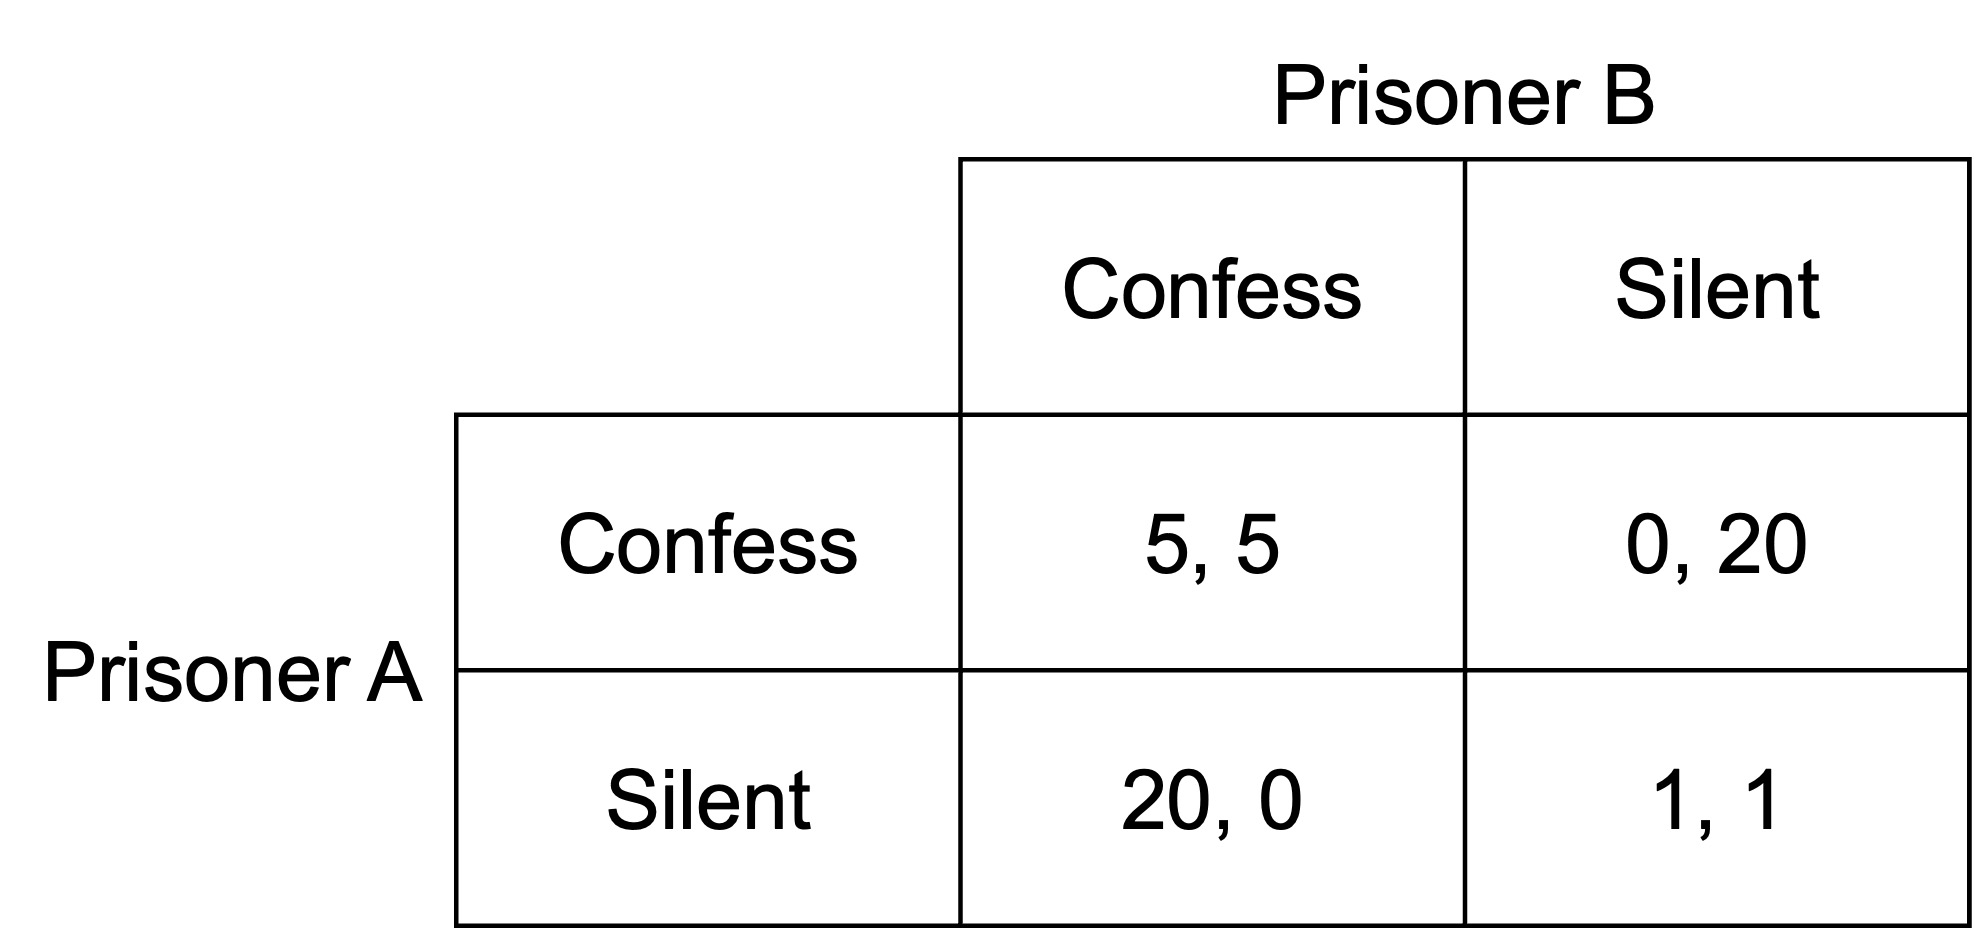
\includegraphics{game-theory/img/prisoners-dilemma-1.jpg}

Prisoners A and B have two actions available: confess and silent. The
numbers in the matrix represent the payoffs from each combination of
actions, in this case the number of years they will serve in prison (a
higher number is a worse outcome). The number in the left of each payoff
cell represents the payoff to the row player, Prisoner A. The number on
the right of each payoff cell is the payoff to the column player,
Prisoner B.

For example, if both Prisoner A and Prisoner B choose to confess, they
each receive a prison sentence of five years. If Prisoner A confesses
and Prisoner B remains silent, Prisoner A gets off without a prison
sentence, whereas Prisoner B gets twenty years.

Equipped with the normal form of the game, we can determine what each
player wants to do in response to each action of the other player.

For example, we can see that if Prisoner B confesses, Prisoner A can
either confess and receive five years in prison, or remain silent and
receive 20 years in prison. They would choose to confess.

We indicate the preferred action in response to another player's action
by circling the relevant payoff. For example:

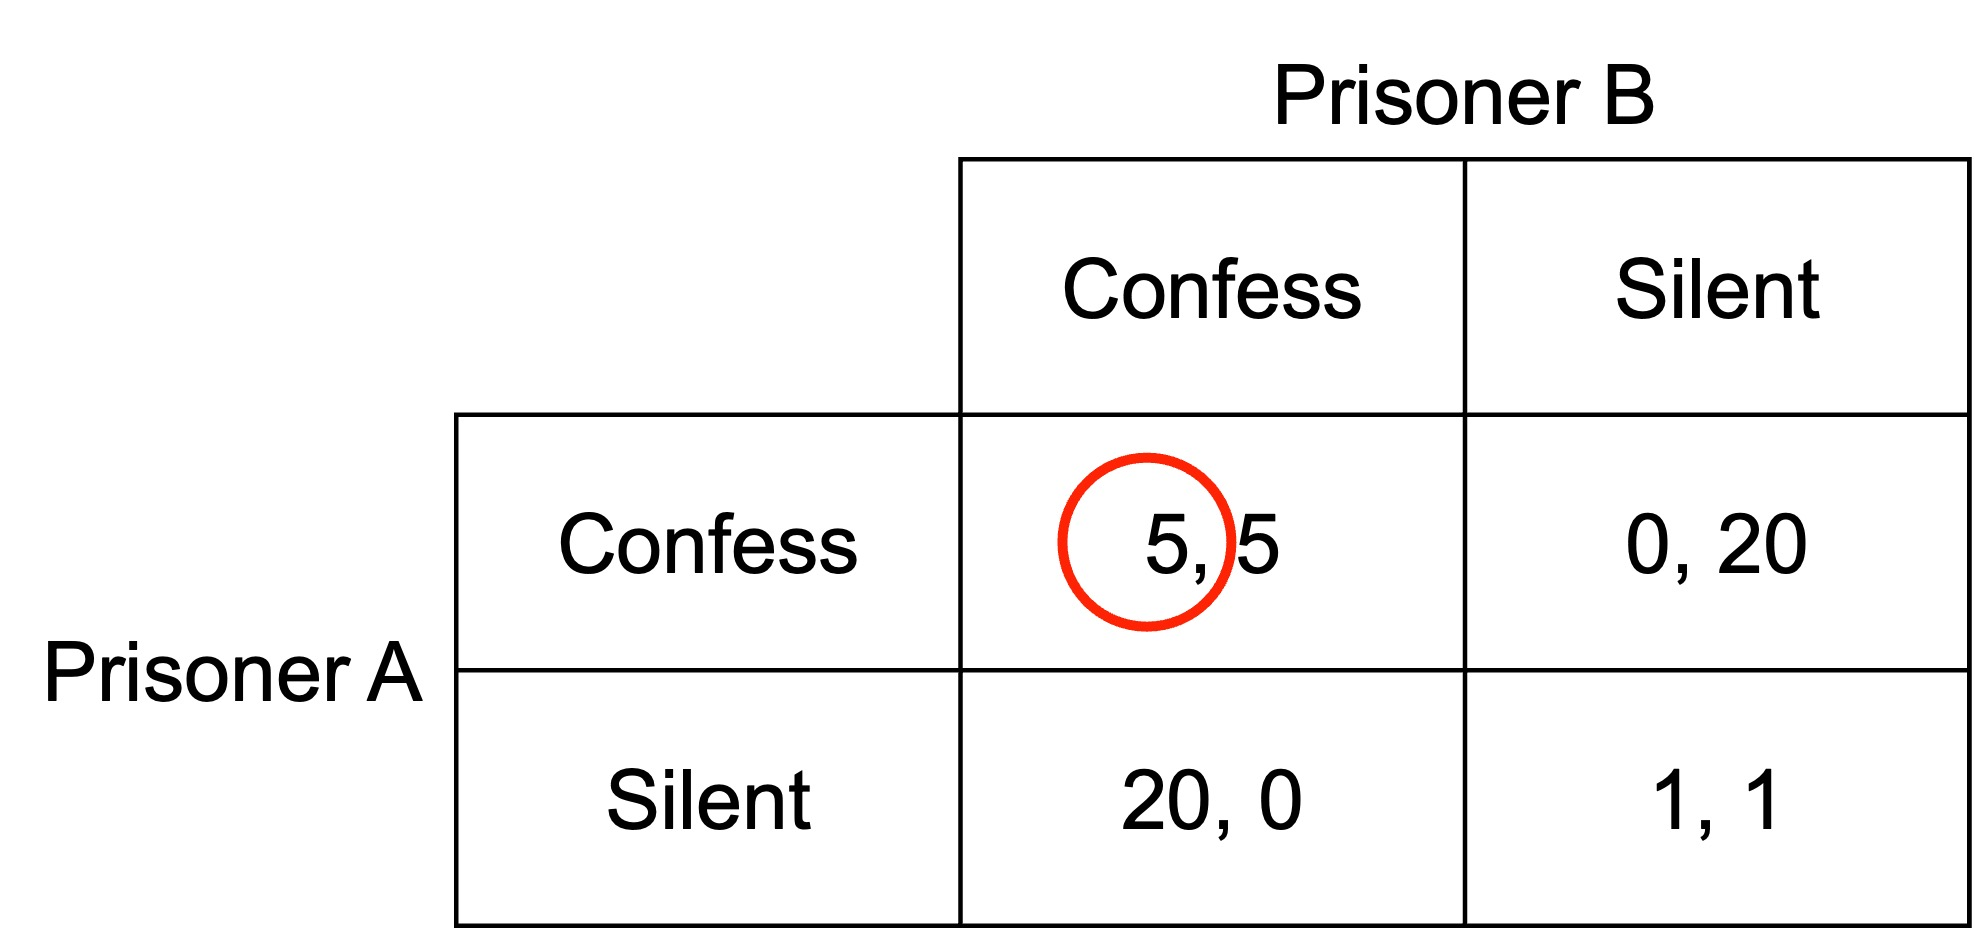
\includegraphics{game-theory/img/prisoners-dilemma-2.jpg}

If Prisoner B remains silent, Prisoner A could either confess and escape
without a sentence, or remain silent and receive a sentence of one year
in prison. They would prefer to confess.

We can then work through the same process for Prisoner B's actions.

If Prisoner A confesses, Prisoner B can either confess and receive five
years in prison, or remain silent and receive 20 years in prison. They
would choose to confess.

If Prisoner A remains silent, Prisoner B could either confess and escape
without a sentence, or remain silent and receive a sentence of one year
in prison. They would prefer to confess.

Indicating this set of preferred actions in response to that of the
other player gives us the following:

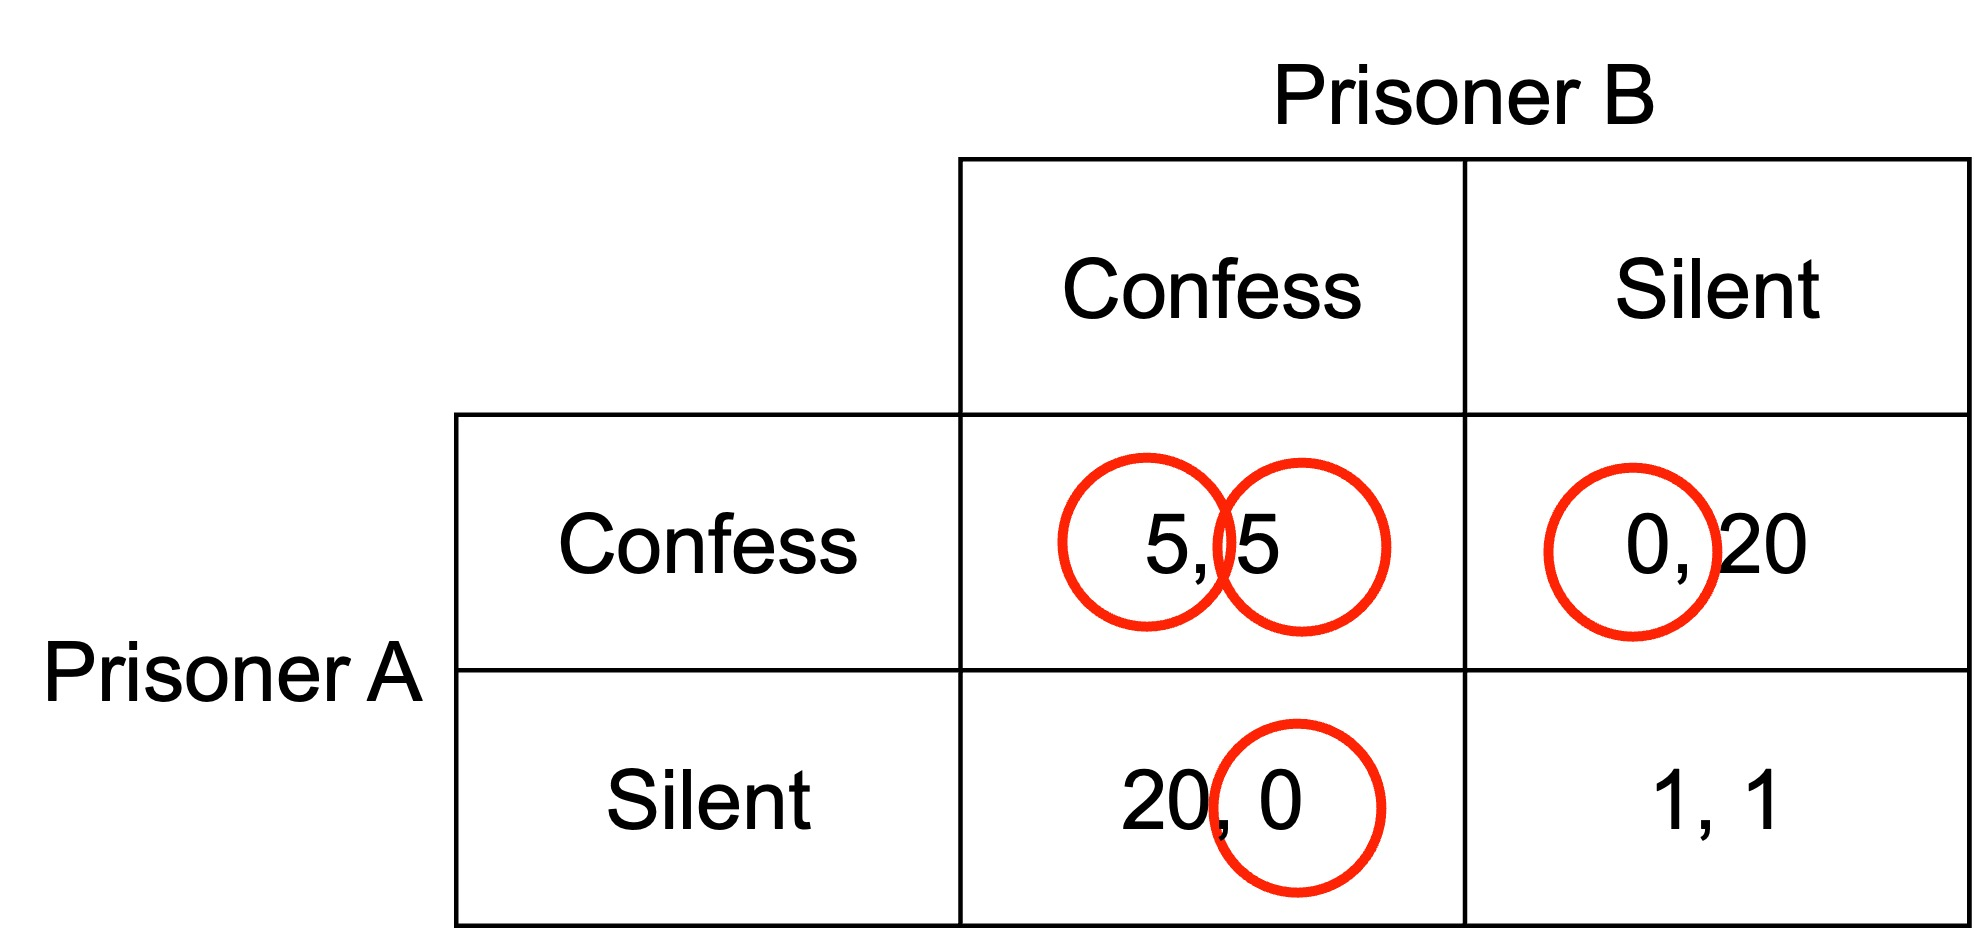
\includegraphics{game-theory/img/prisoners-dilemma-3.jpg}

\hypertarget{dominant-strategies}{%
\section{Dominant strategies}\label{dominant-strategies}}

A strategy is (strictly) dominant if it gives a (strictly) higher payoff
than every other strategy, for every strategy that your rivals play.

If you have a strictly dominant strategy, you should play it for sure.

In a dominant strategy equilibrium, all players choose a dominant
strategy.

In the prisoner's dilemma both players have a dominant strategy to
confess.

\hypertarget{nash-equilibrium}{%
\section{Nash equilibrium}\label{nash-equilibrium}}

A set of strategies is a Nash equilibrium if every player is playing a
best response to their rivals' strategies. No one has an incentive to
change strategy.

A Nash equilibrium is self-enforcing and stable.

An agreement that is a Nash equilibrium is self-fulfilling. If the
players agree to play a certain way, they'll both go through with it.
Unilateral deviations are not worthwhile.

The prisoner's dilemma has a single Nash equilibrium: (Confess,
Confess). Visually, where the preferred response of both players to the
other player's action falls within the same cell, this indicates a Nash
equilibrium.

\hypertarget{simultaneous-move-one-shot-game-examples}{%
\section{Simultaneous move one-shot game
examples}\label{simultaneous-move-one-shot-game-examples}}

\hypertarget{the-driving-game}{%
\subsection{The driving game}\label{the-driving-game}}

Consider the following game between two players deciding what side of
the road to drive on. If they don't drive on the same side of the road
they crash.

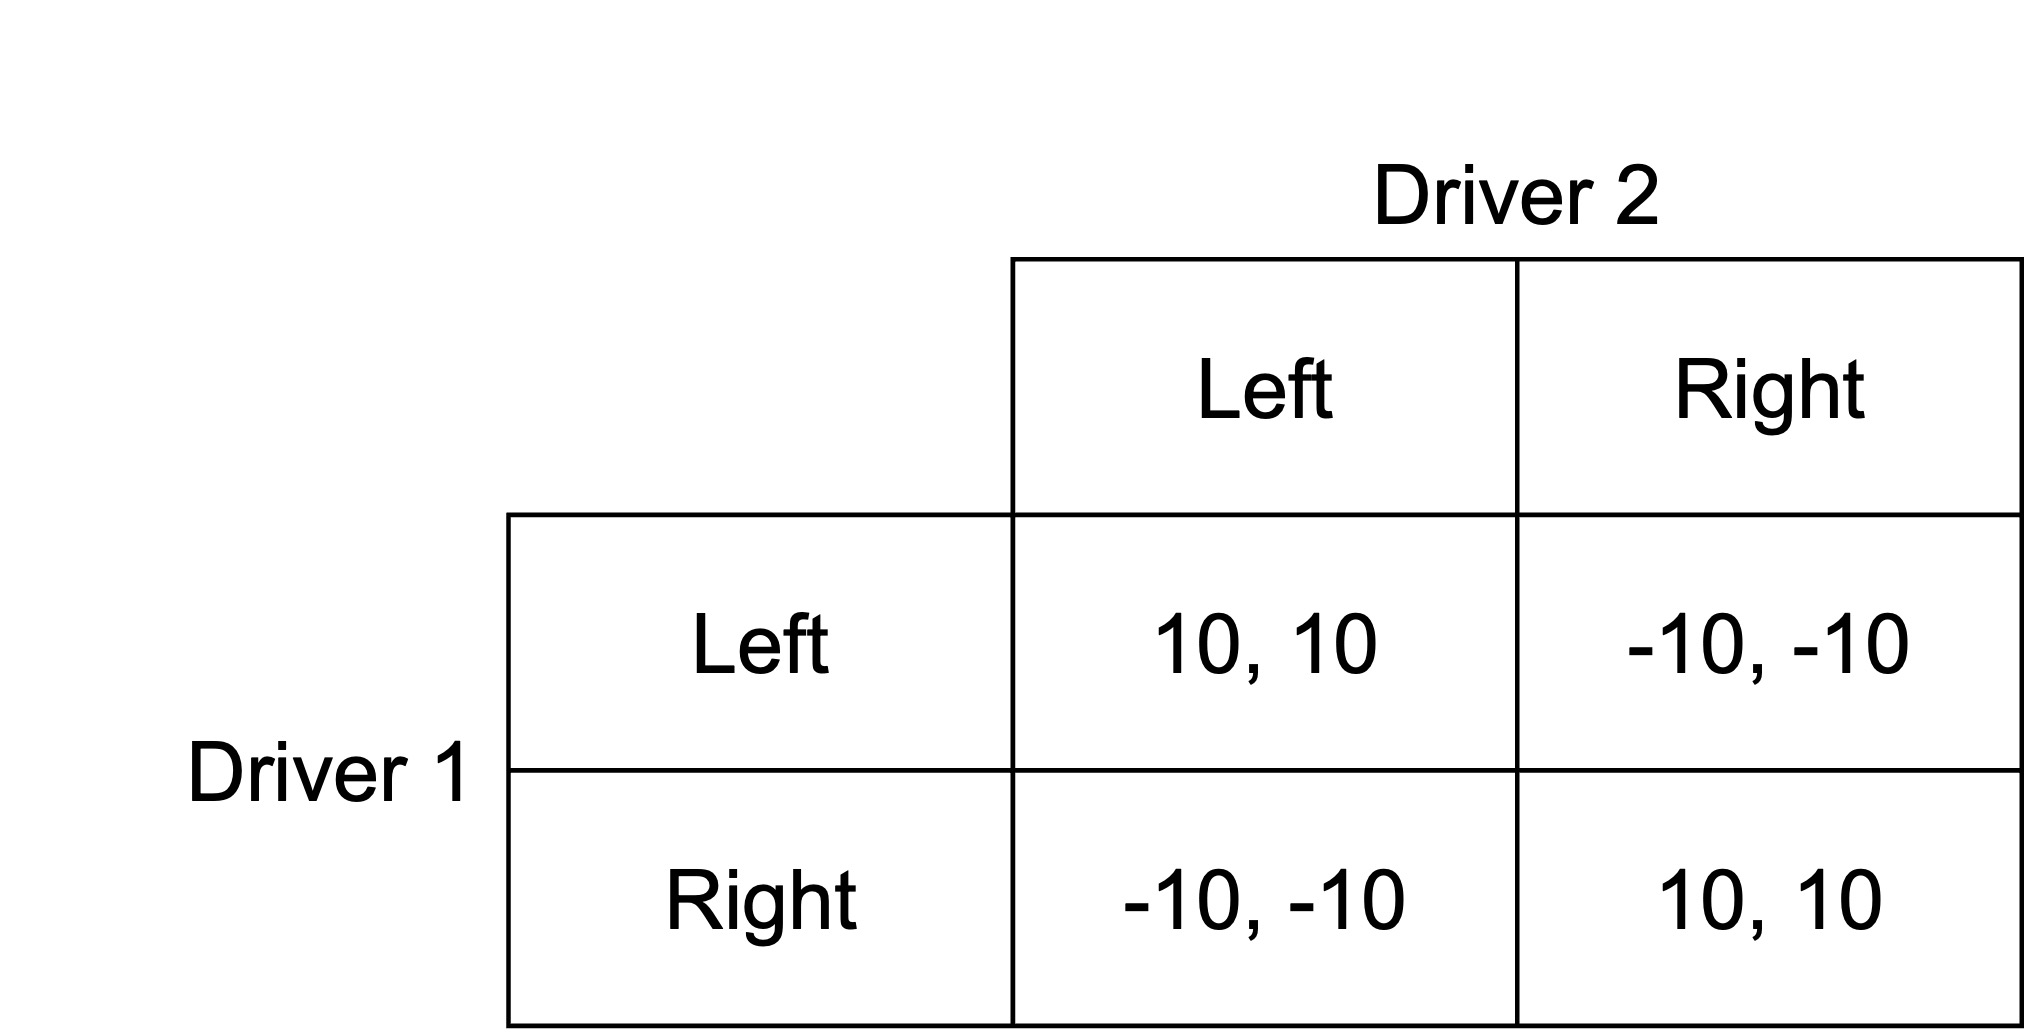
\includegraphics{game-theory/img/driving-game-1.jpg}

What are the Nash equilibria? The Nash equilibria are (Left, Left) and
(Right, Right).

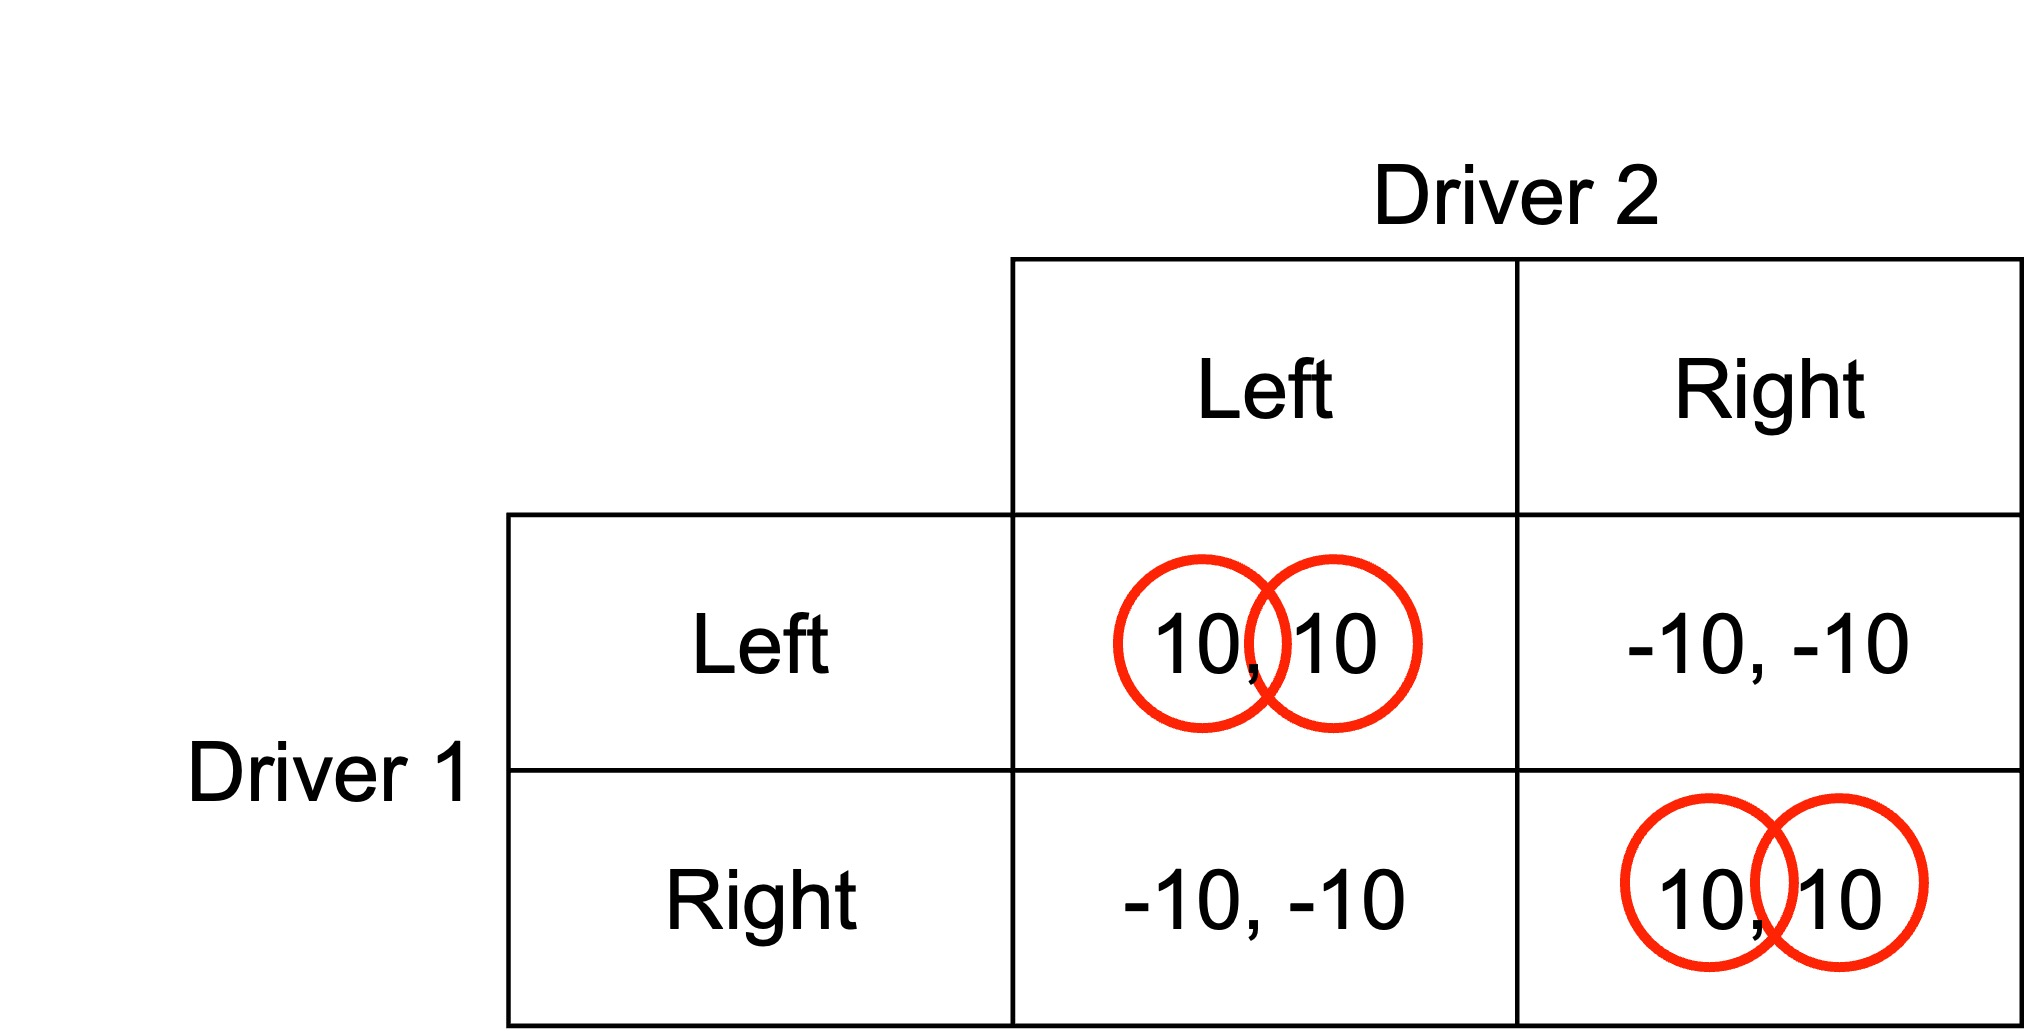
\includegraphics{game-theory/img/driving-game-2.jpg}

\hypertarget{matching-pennies}{%
\subsection{Matching pennies}\label{matching-pennies}}

Consider the following game between two players, Even and Odd. If both
pennies match, Even wins. If they don't match, Odd wins.

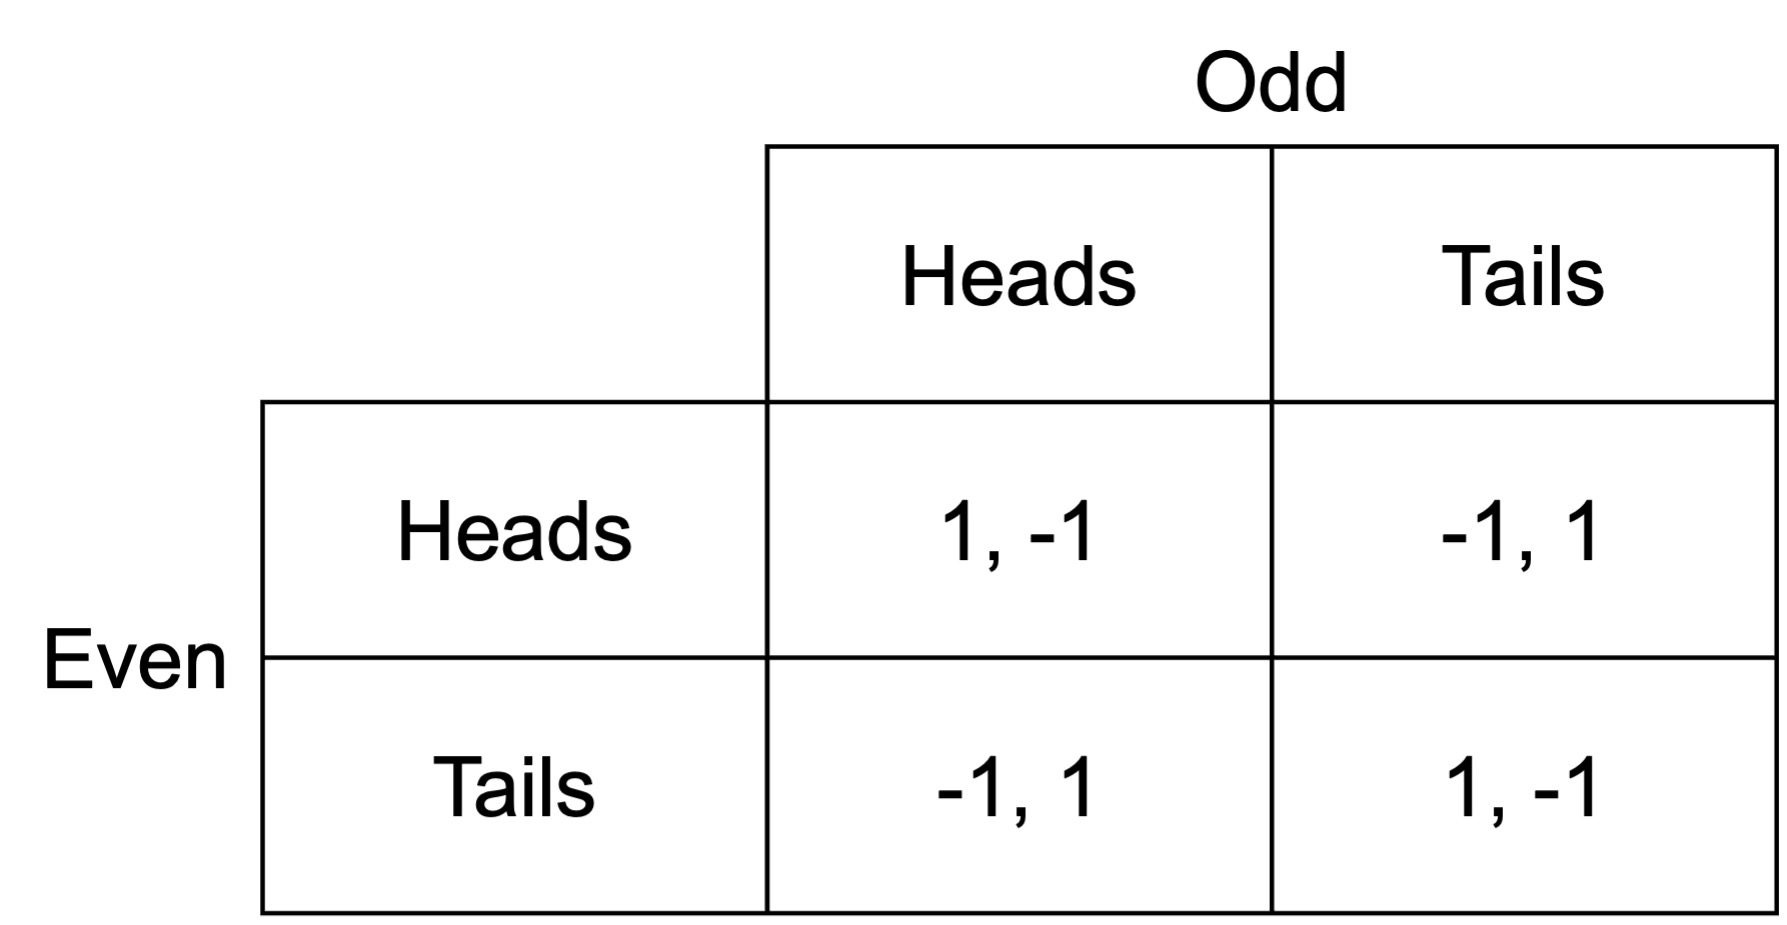
\includegraphics{game-theory/img/matching-pennies-1.jpg}

What are the Nash equilibria?

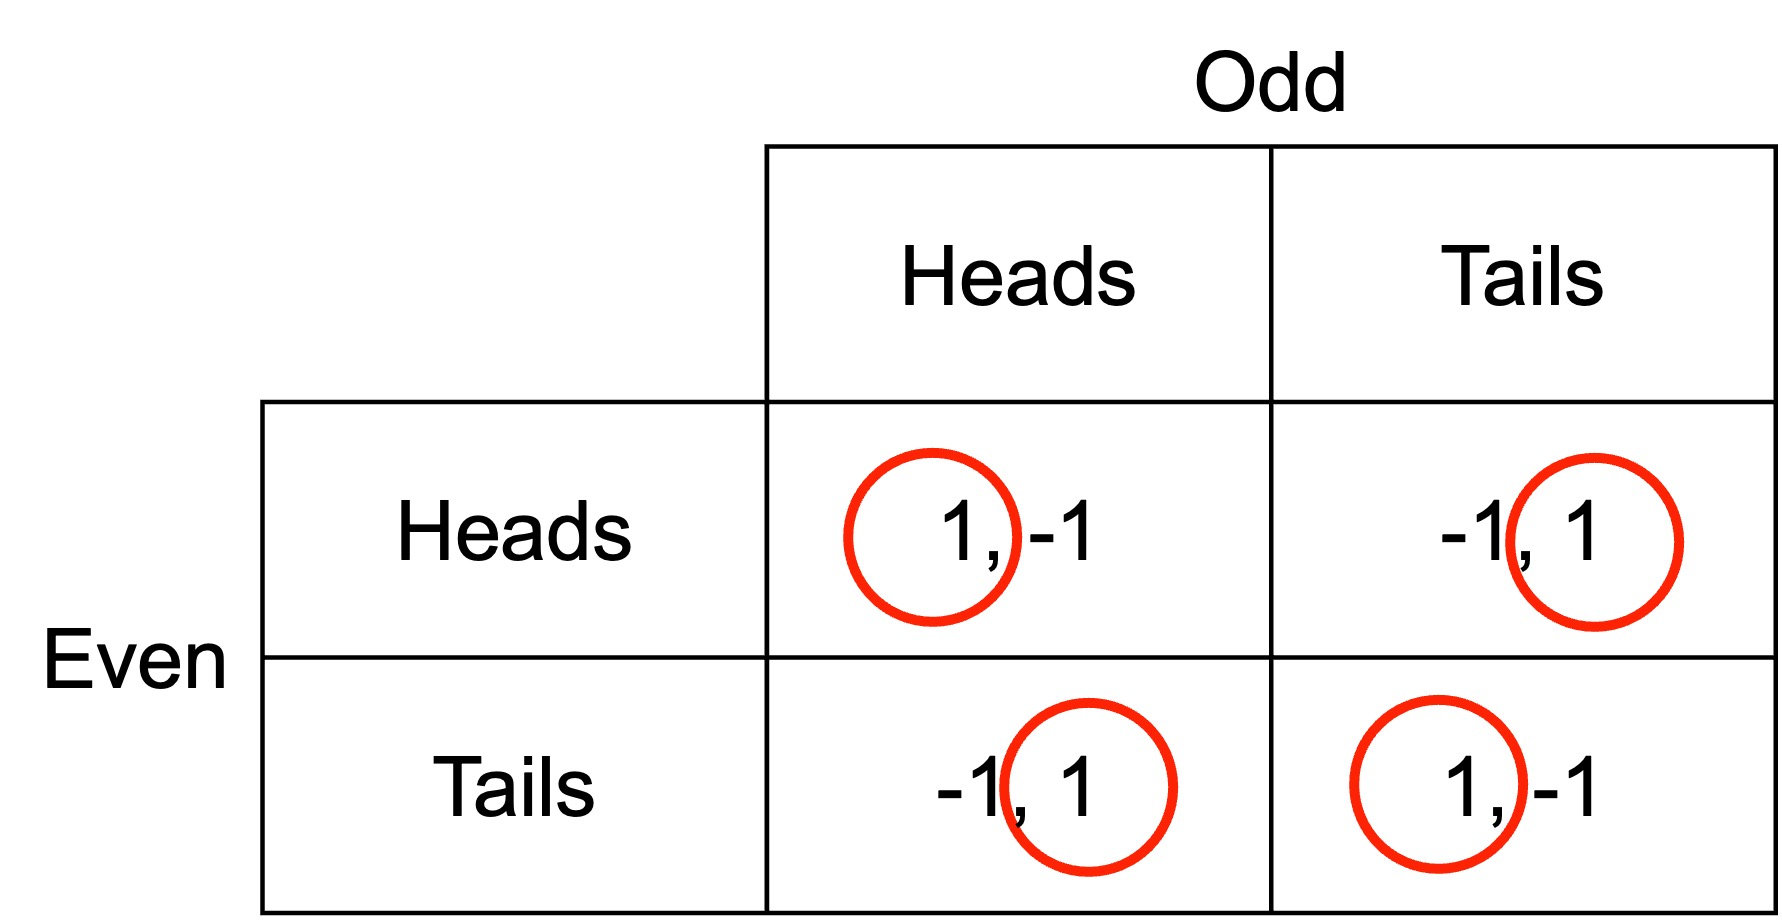
\includegraphics{game-theory/img/matching-pennies-2.jpg}

There are no pure-strategy Nash equilibria for this game. (There are
mixed-strategy equilibria, but mixed-strategy equilibria are beyond the
scope of this subject.)

\hypertarget{the-stag-hunt}{%
\subsection{The stag hunt}\label{the-stag-hunt}}

Consider the following game between two players deciding what animal
they will hunt. Both hunters need to cooperate to catch the stag. They
can catch a hare by themselves, but it provides less meat.

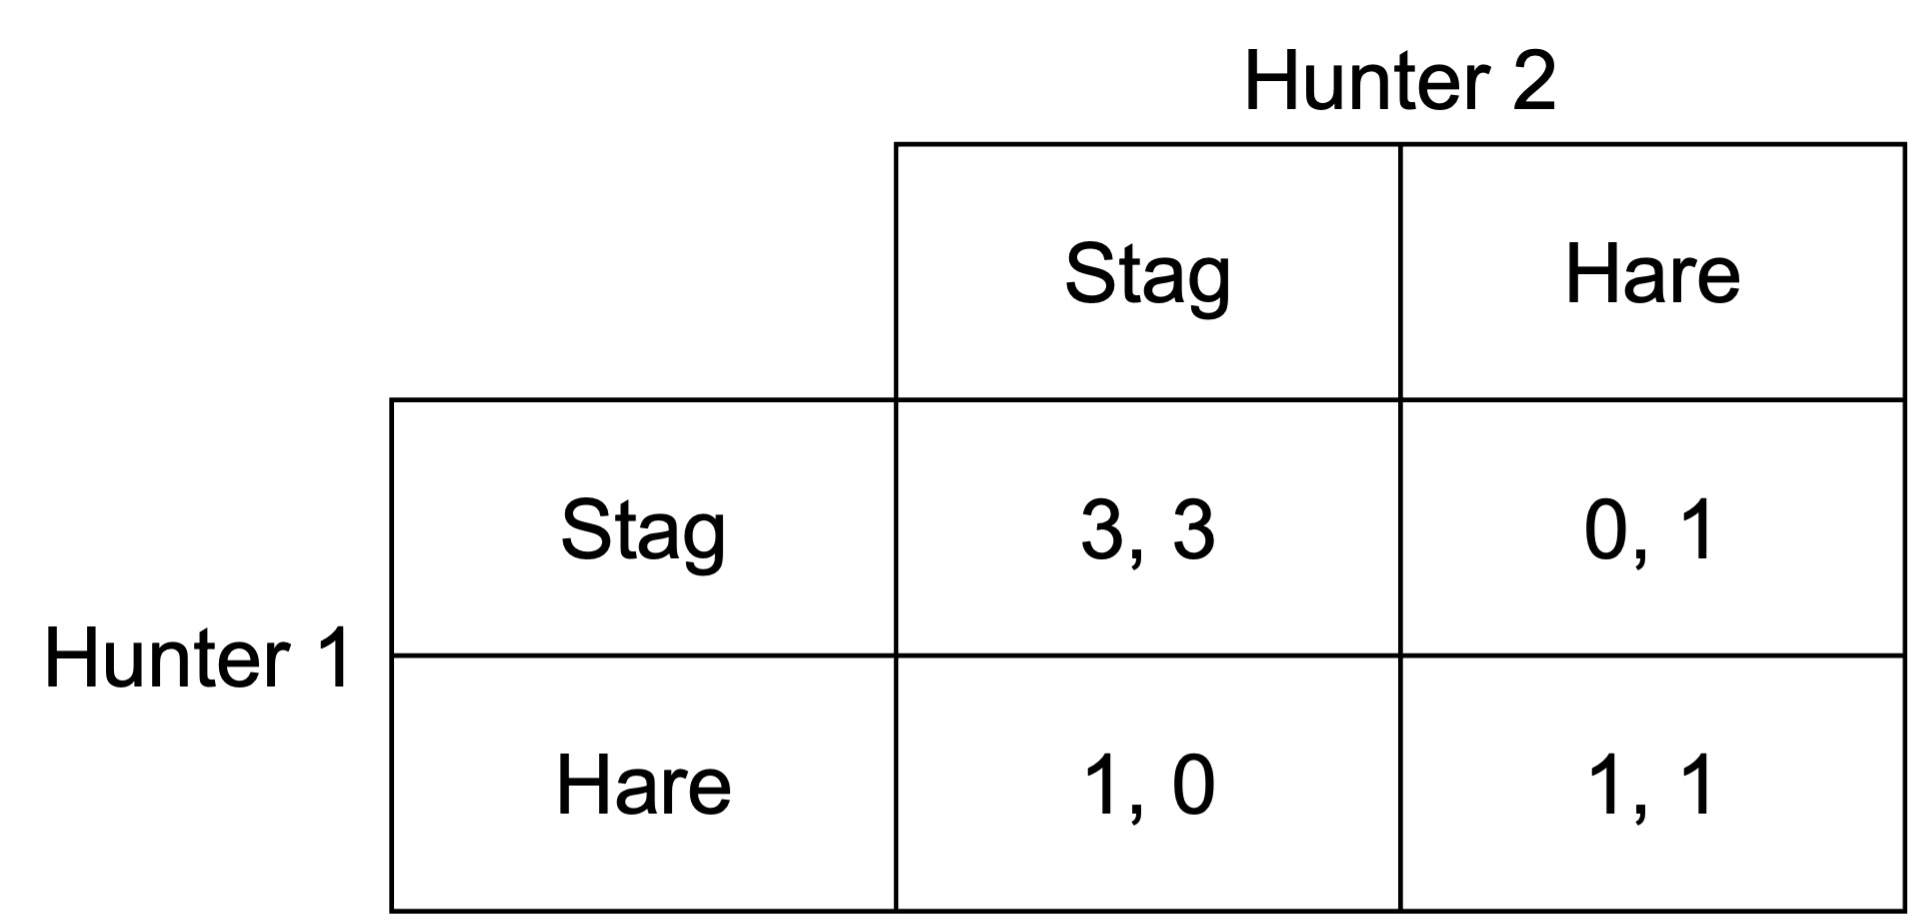
\includegraphics{game-theory/img/stag-hunt-1.jpg}

What are the Nash equilibria?

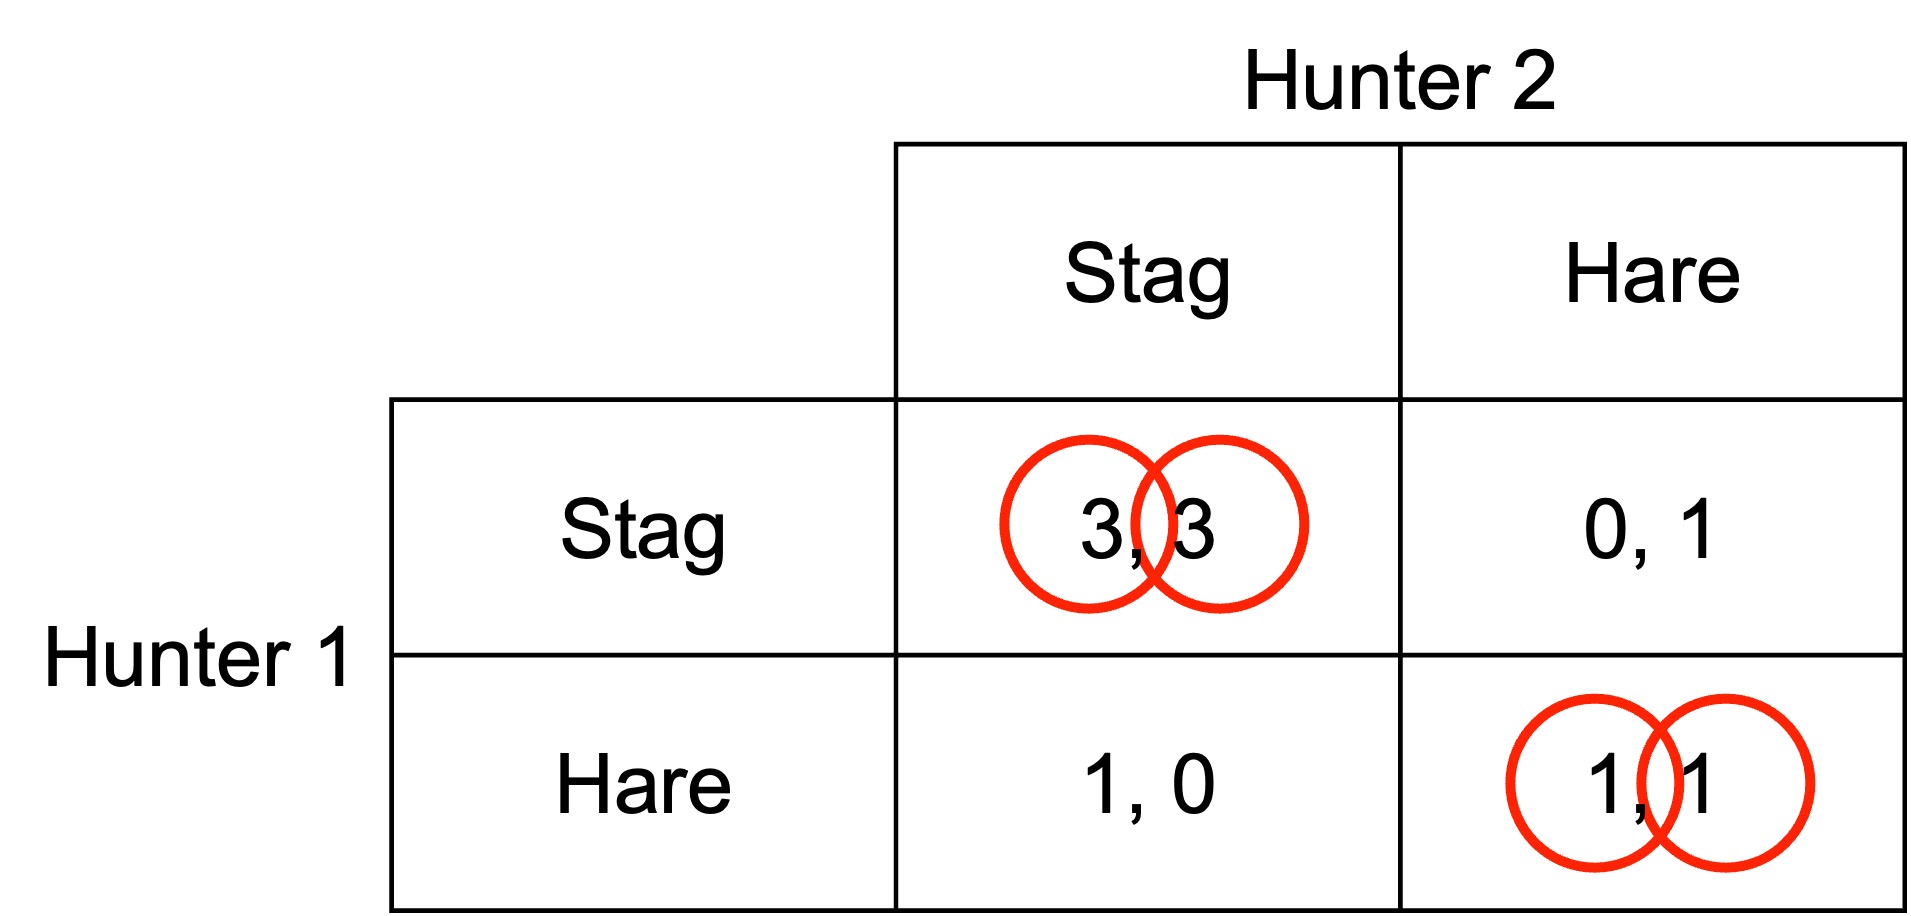
\includegraphics{game-theory/img/stag-hunt-2.jpg}

The Nash equilibria are (Stag, Stag) and (Hare, Hare).

\hypertarget{the-public-goods-game}{%
\subsection{The public goods game}\label{the-public-goods-game}}

Participants are given an initial endowment.

Each secretly and simultaneously chooses how much of their endowment
they wish to contribute to a public pot.

The money in the public pot is multiplied by some amount \(m\) and split
evenly between the players.

For example, players might each be given \$10, with the pot doubled.

In Nash equilibrium in the public goods game, nobody transfers anything
to the pot. Any contributions are split between all players, so if there
are more players than \(m\) (which is normally the case by design),
contributions result in a loss.

The Pareto optimal result, however, is for all players to contribute
their full endowment and each receive back their contribution multiplied
by \(m\).

\hypertarget{sequential-games}{%
\chapter{Sequential games}\label{sequential-games}}

In sequential games, players make sequential decisions knowing the
action of the other player.

\hypertarget{the-extensive-form}{%
\section{The extensive form}\label{the-extensive-form}}

The extensive form representation explicitly shows the timing of play.

Payoffs are represented in a game tree.

I will now illustrate the extensive form of the game with a game called
the centipede game.

\hypertarget{the-centipede-game}{%
\subsection{The centipede game}\label{the-centipede-game}}

This centipede game has six stages. At each stage, a player can ``take''
and end the game or they can ``pass'', increasing the total payoff. The
other player then has a move.

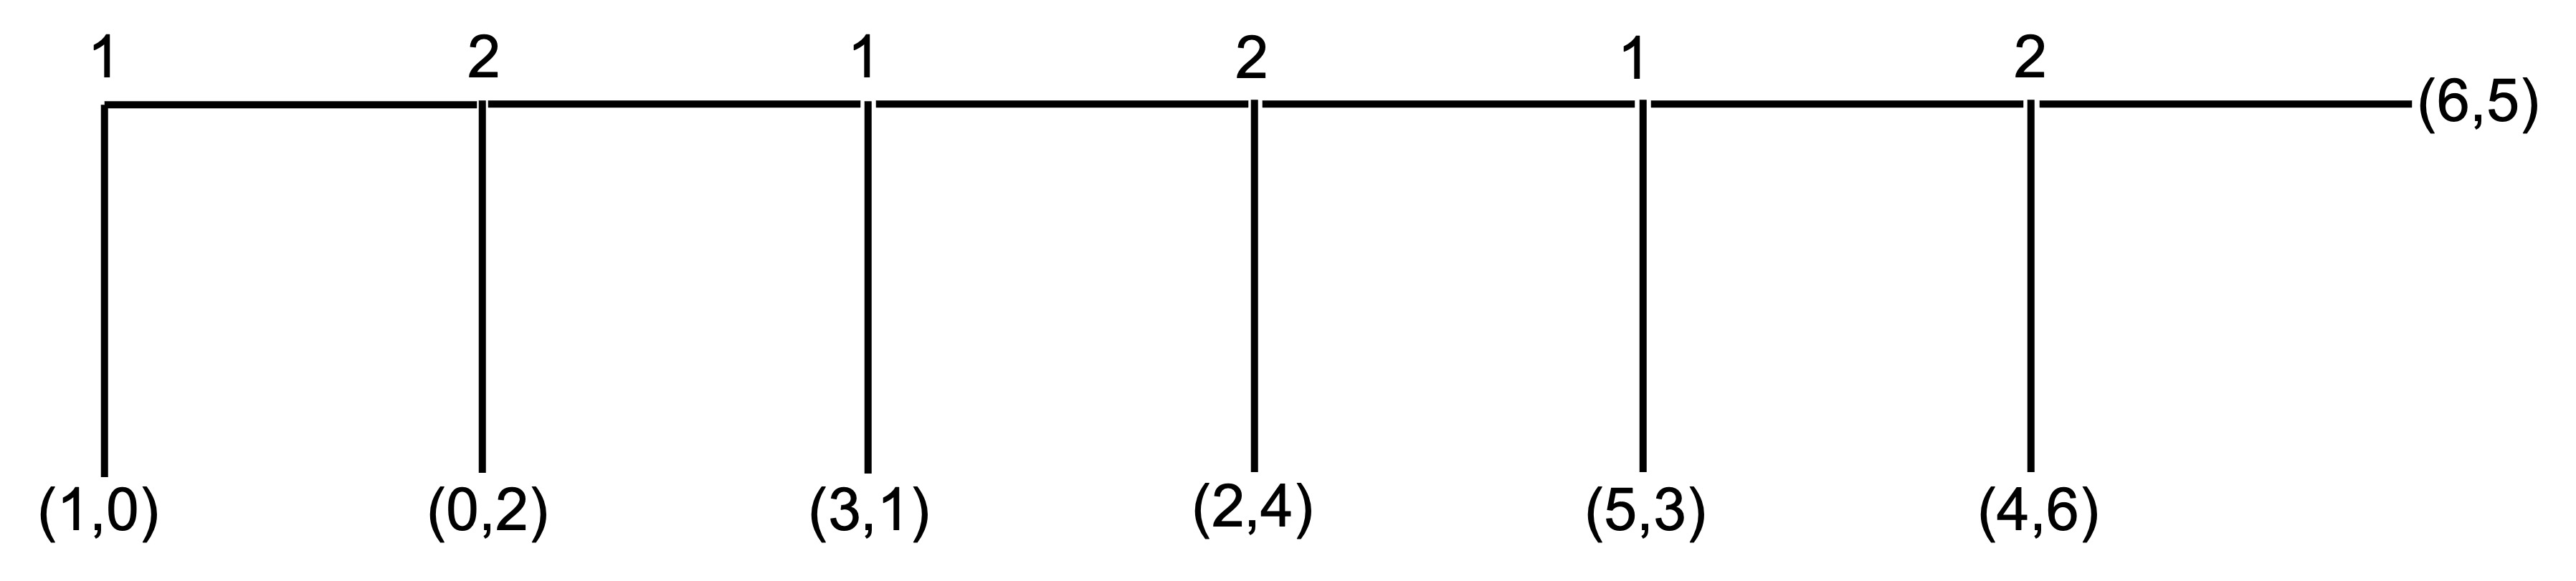
\includegraphics{game-theory/img/centipede-game-1.jpg}

\hypertarget{subgame-perfect-nash-equilibrium}{%
\section{Subgame perfect Nash
equilibrium}\label{subgame-perfect-nash-equilibrium}}

A subgame is a part of a game that can be played as a game itself. It
begins at a single node and contains every successor node.

A Nash Equilibrium is subgame perfect if every player plays the Nash
Equilibrium in every subgame

We can solve for the subgame perfect Nash equilibrium of sequential
games by backward induction:

\begin{itemize}
\item
  solve for the decision nodes at the end of the game first
\item
  work your way to the beginning of the game.
\end{itemize}

In our centipede game, using backward induction, player 2 at the final
stage will take for a payoff of 6 (relative to 5 for passing).

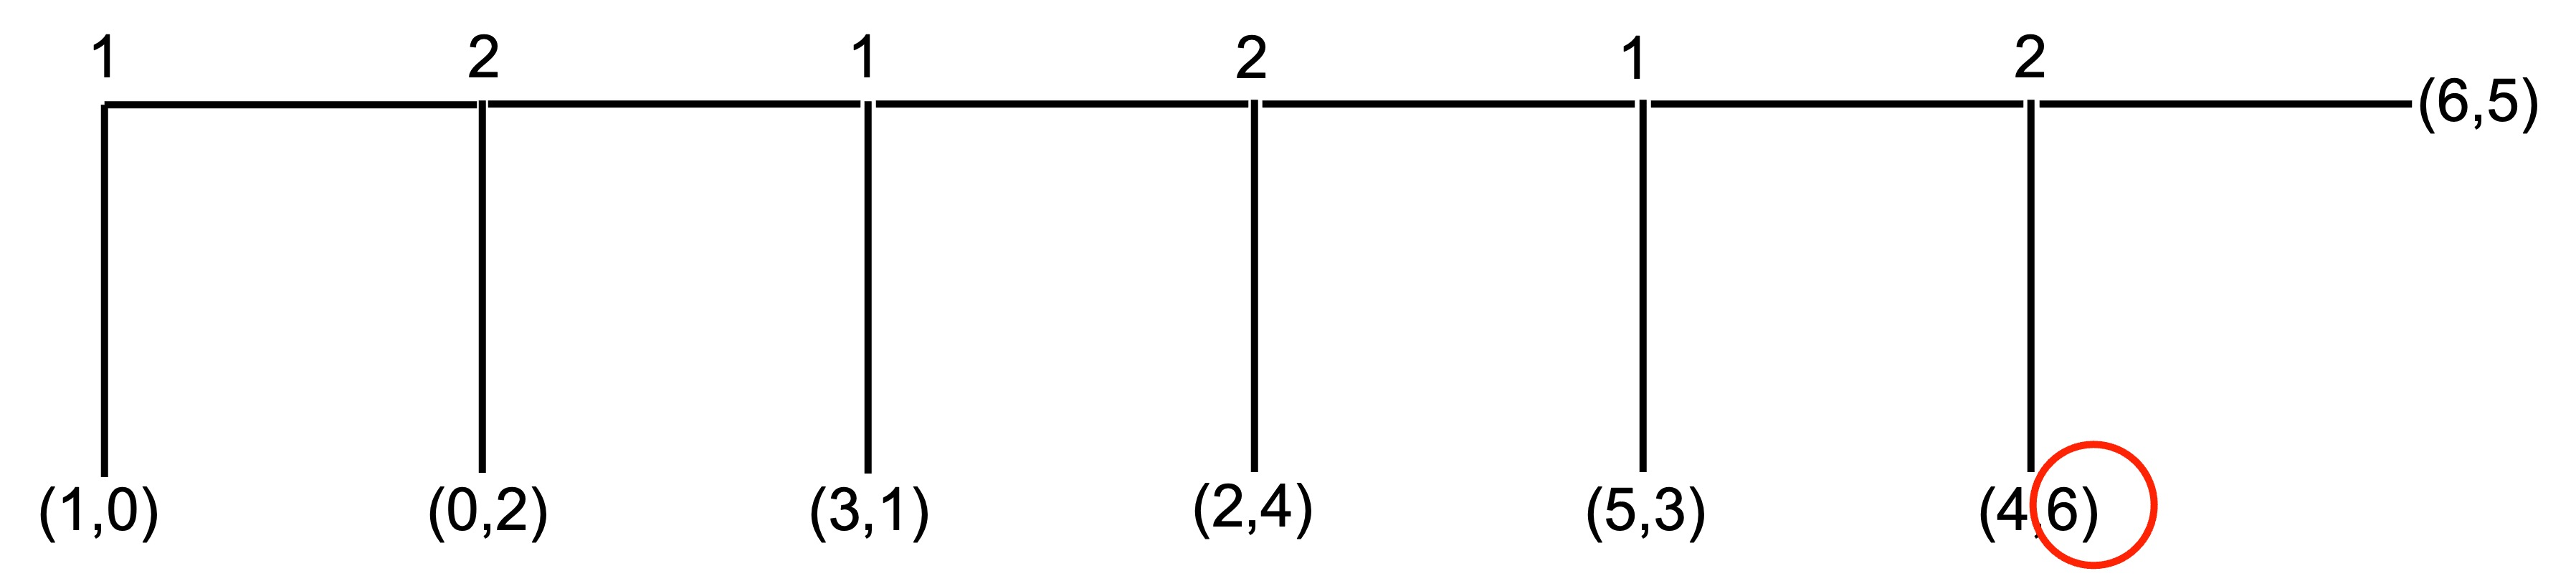
\includegraphics{game-theory/img/centipede-game-2.jpg}

Therefore, player 1 at the stage before will take for a payoff of 5
(relative to the payoff of 4 they would receive for passing, given
player 2 will then take).

Therefore, player 2 at the stage before will take for a payoff of 4.

And so on.

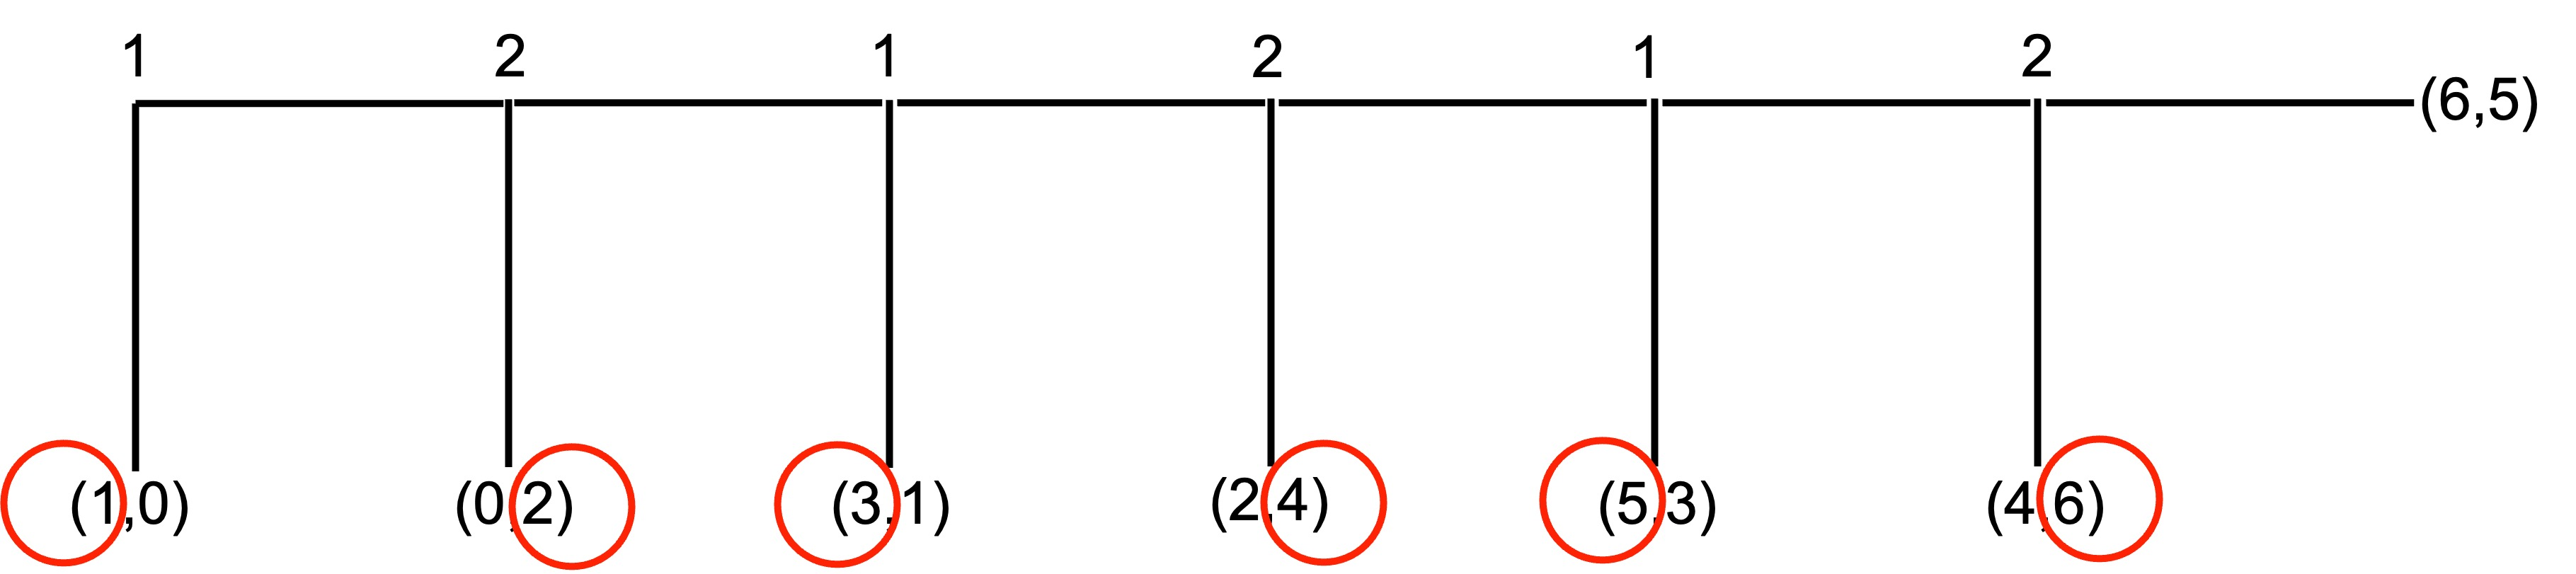
\includegraphics{game-theory/img/centipede-game-3.jpg}

There is a unique subgame perfect equilibrium:
\(S_1=(\text{take, take, take})\) and \(S_2=(\text{take, take, take})\),
where \(S_1\) and \(S_2\) are the set of strategies for player 1 and
player 2 respectively.

In the subgame perfect Nash equilibrium, player 1 takes at the first
stage.

\hypertarget{sequential-game-examples}{%
\section{Sequential game examples}\label{sequential-game-examples}}

\hypertarget{the-ultimatum-game}{%
\subsection{The ultimatum game}\label{the-ultimatum-game}}

The ultimatum game involves two players: the proposer and the responder.

The proposer is given a fixed amount of money \(m\). They then offer a
portion \(x\) of the sum \(m\) to the responder.

The responder can either accept of reject the offer. They make this
decision knowing \(m\) and \(x\).

If the responder accepts, the responder receives \(x\) and the proposer
gets \(m-x\). If the responder rejects, both players receive nothing.

Below is the extensive form of the ultimatum game with \(m=\$10\) and an
assumption that the offer must be a whole dollar amount.

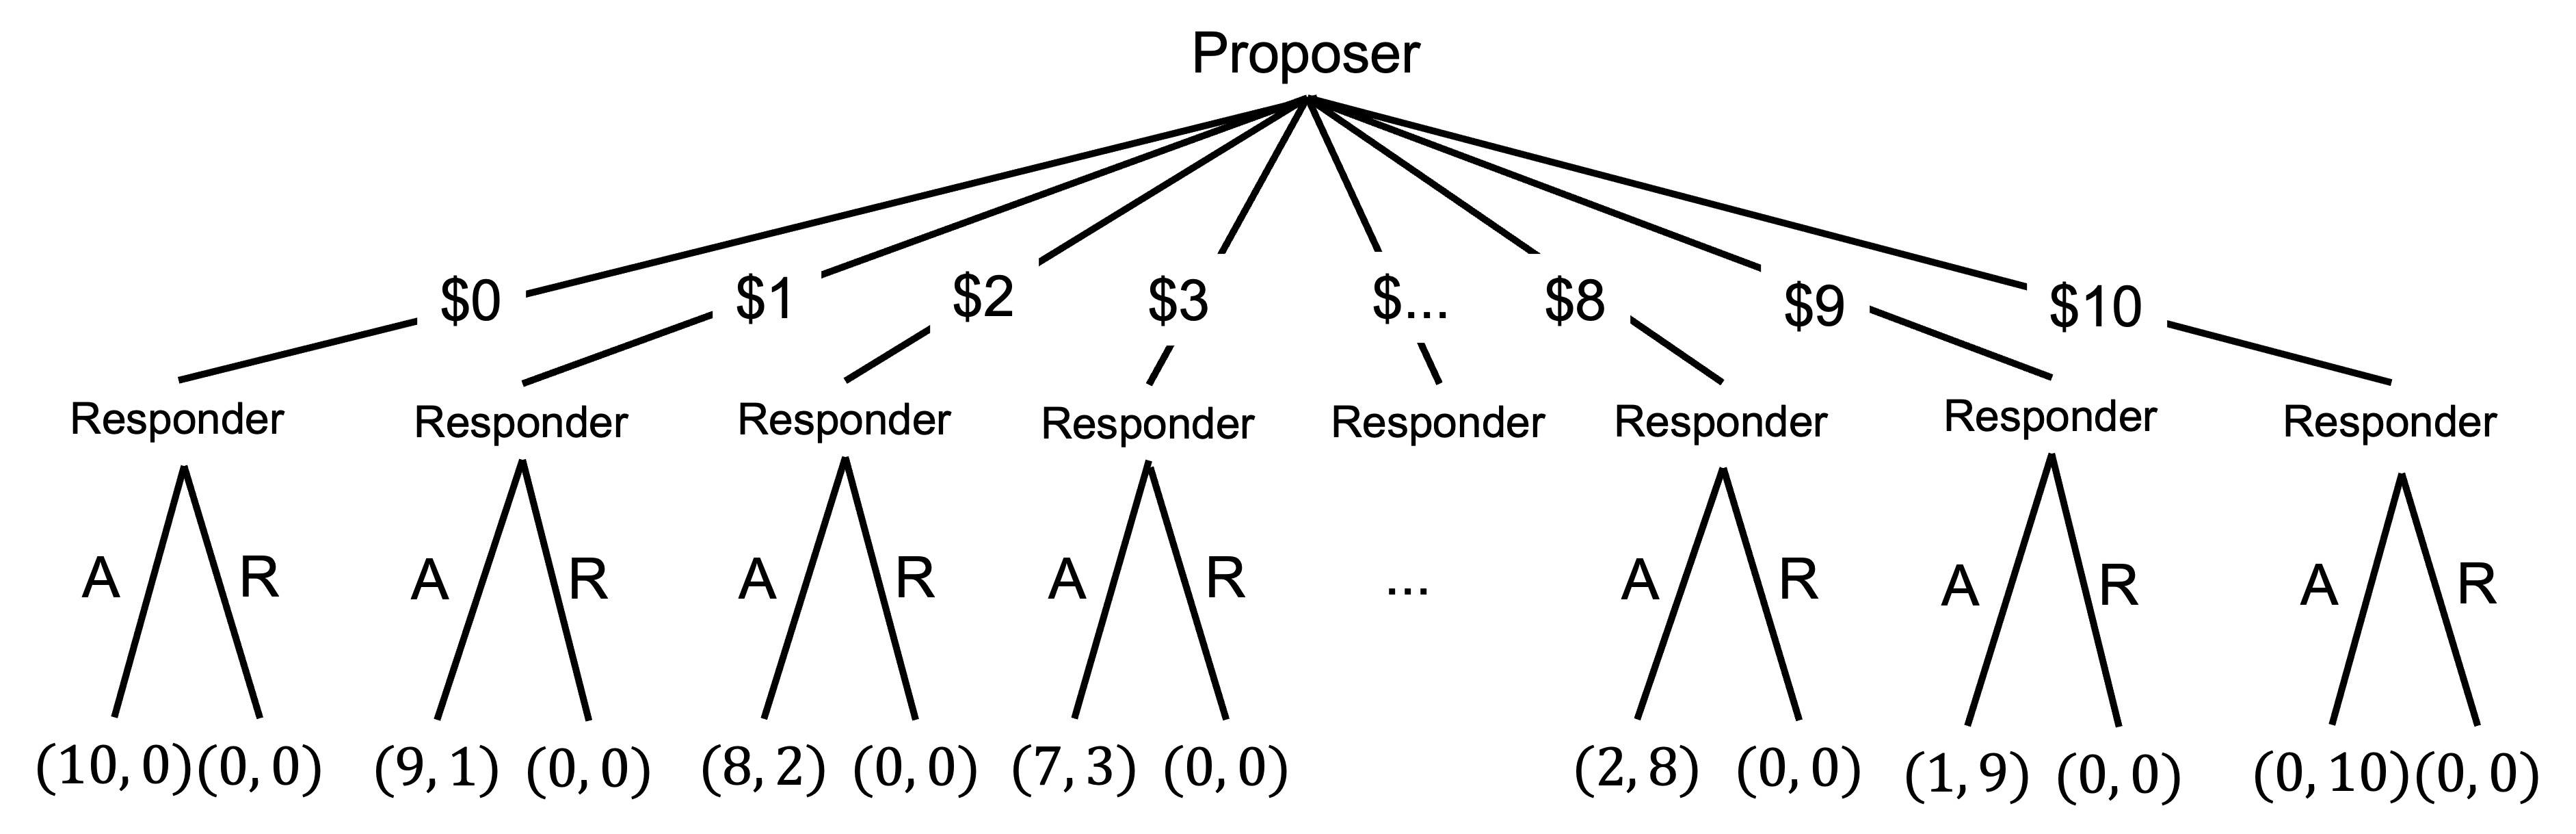
\includegraphics{game-theory/img/ultimatum-game-1.jpg}

If we work through this game by backward induction, we can see that for
any non-zero amount, the responder will accept the offer. The only time
they might not accept is there the offer is \(0\).

Given this, the proposer will offer \(\$1\) only.

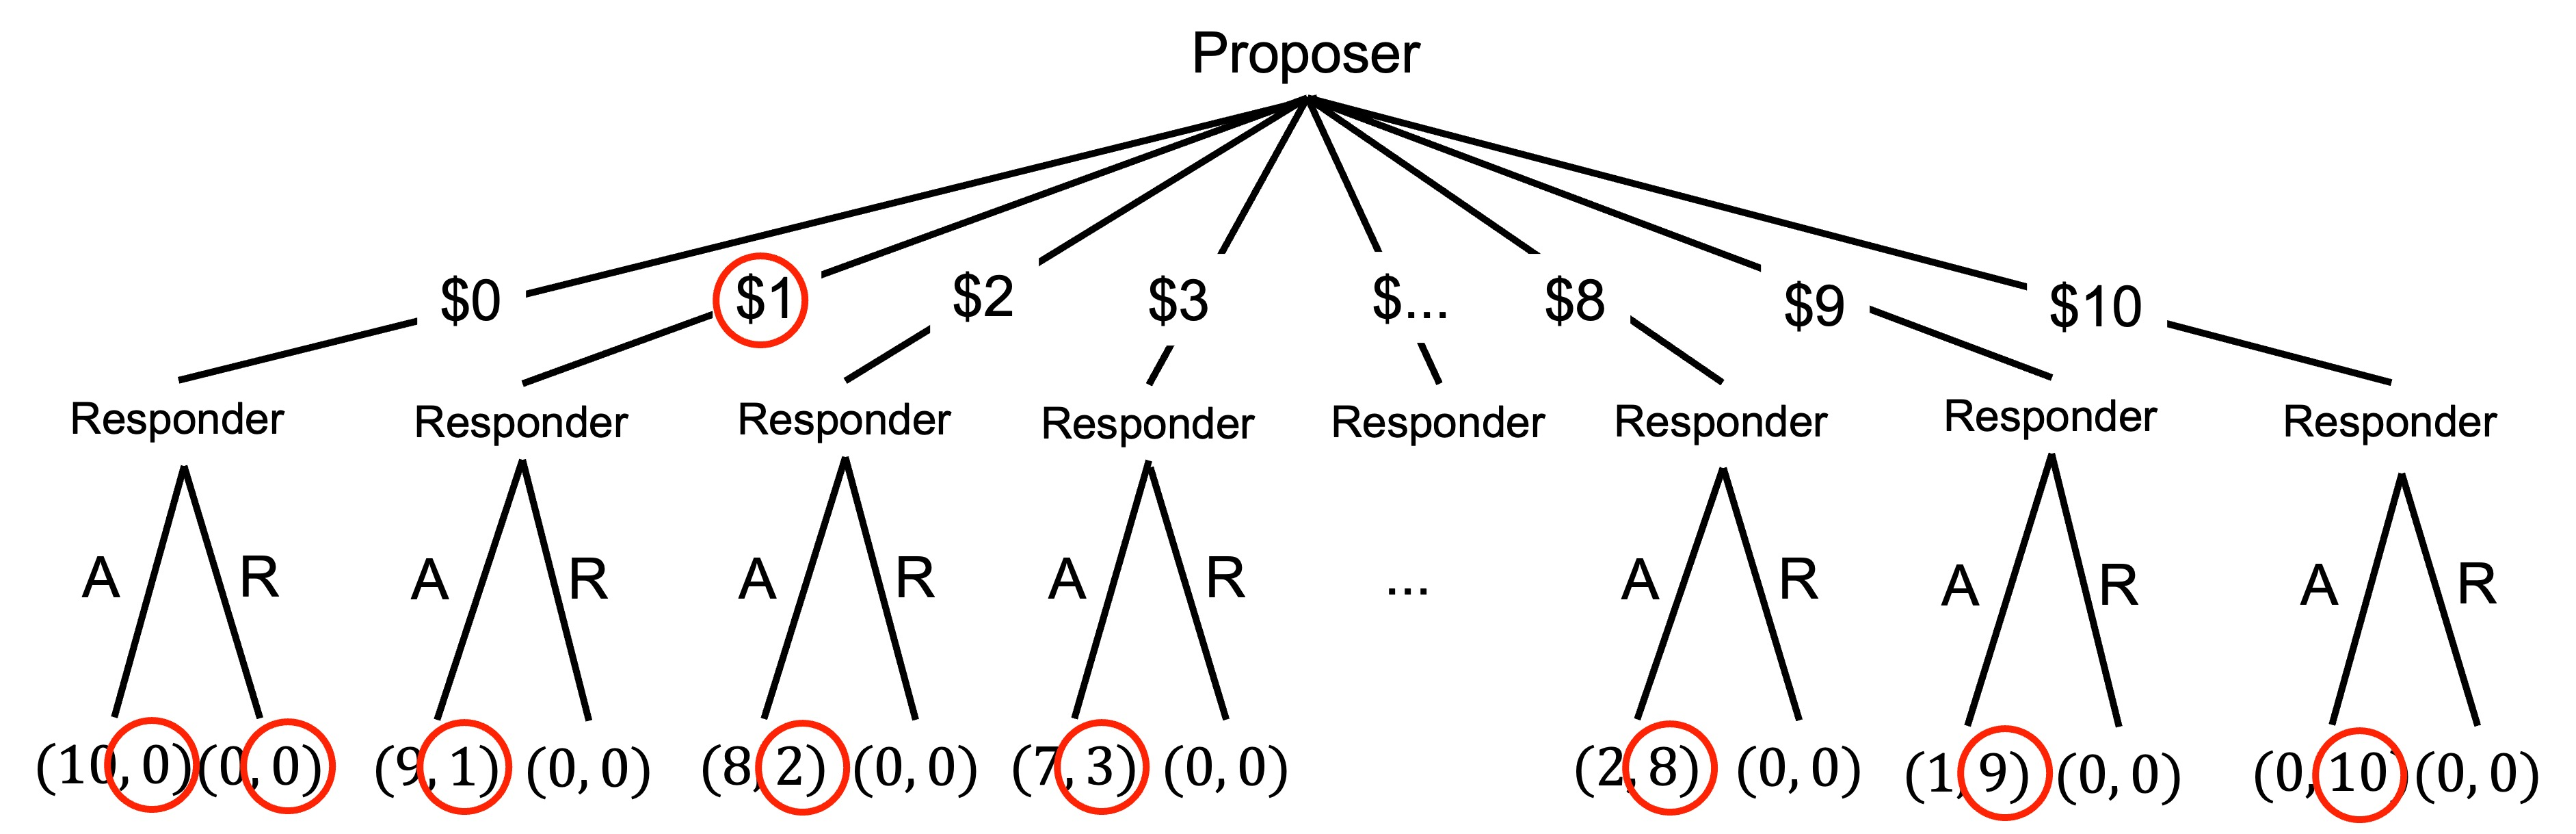
\includegraphics{game-theory/img/ultimatum-game-2.jpg}

More generally, game theory makes a clear prediction on the outcome of
the ultimatum game. If the players have monotonic preferences and the
offer strategy set is discrete:

\begin{itemize}
\item
  The responder accepts any \(x>0\).
\item
  The proposer offers \(x=\epsilon\), where \(\epsilon\) is the smallest
  non-zero amount the proposer can offer.
\end{itemize}

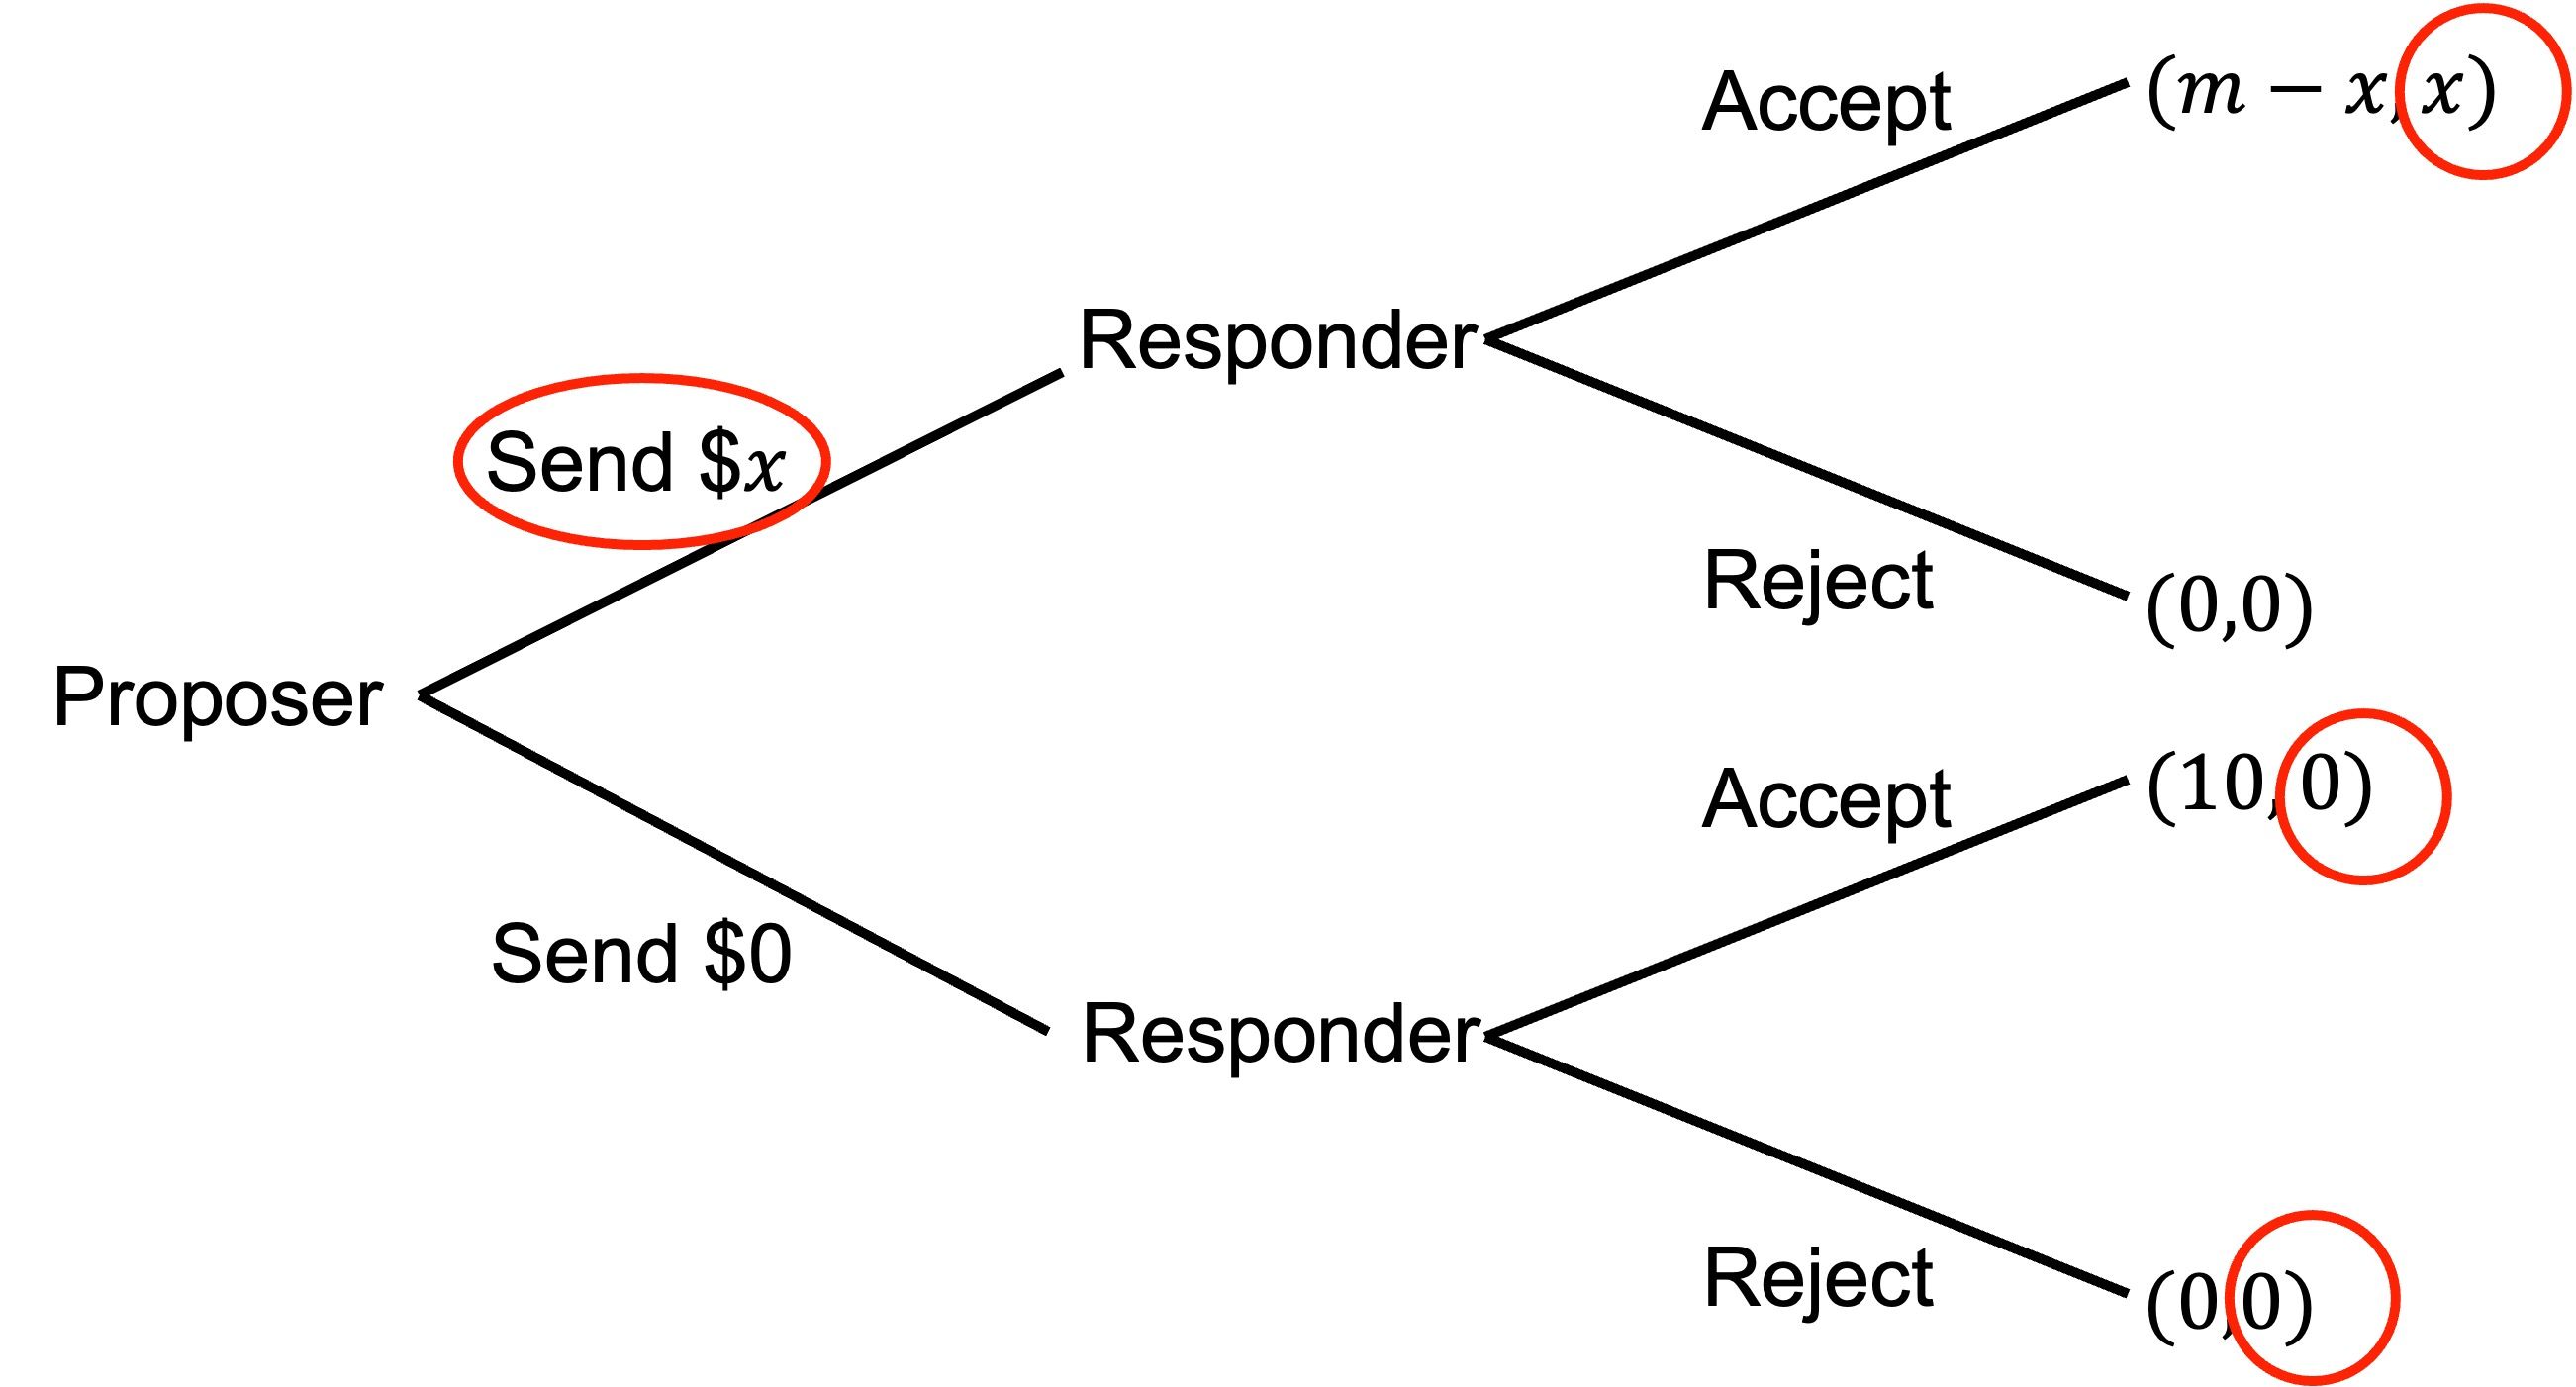
\includegraphics{game-theory/img/ultimatum-game-3.jpg}

The other (weak) subgame perfect Nash equilibrium is an offer of \$0 and
acceptance.

Where the strategy space is continuous (i.e \(\epsilon\) could always be
made smaller) the only subgame perfect Nash equilibrium is for the
proposer to offer \$0 and the receiver to accept.

\hypertarget{the-dictator-game}{%
\subsection{The dictator game}\label{the-dictator-game}}

In the dictator game, the dictator is given a fixed amount of money 𝑚.
They then offer a portion 𝑥 of the sum 𝑚 to the receiver. The game then
ends.

Exchange is unilateral. Receivers have an empty strategy set.

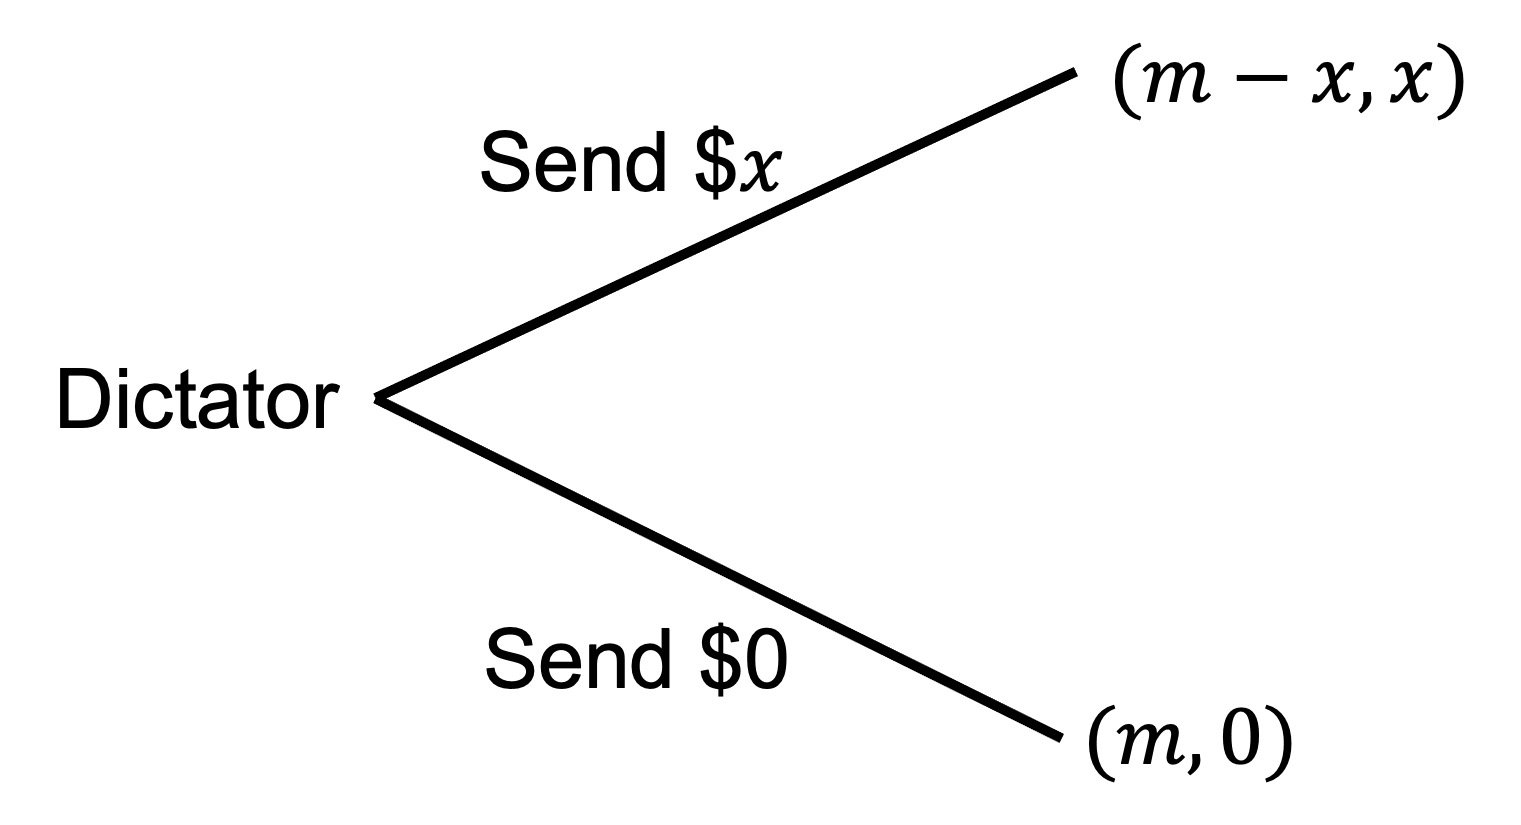
\includegraphics{game-theory/img/dictator-game-1.jpg}

The standard game theory prediction is no interaction whatsoever. The
dictator maximises their payoff by keeping all of the endowment
themselves.

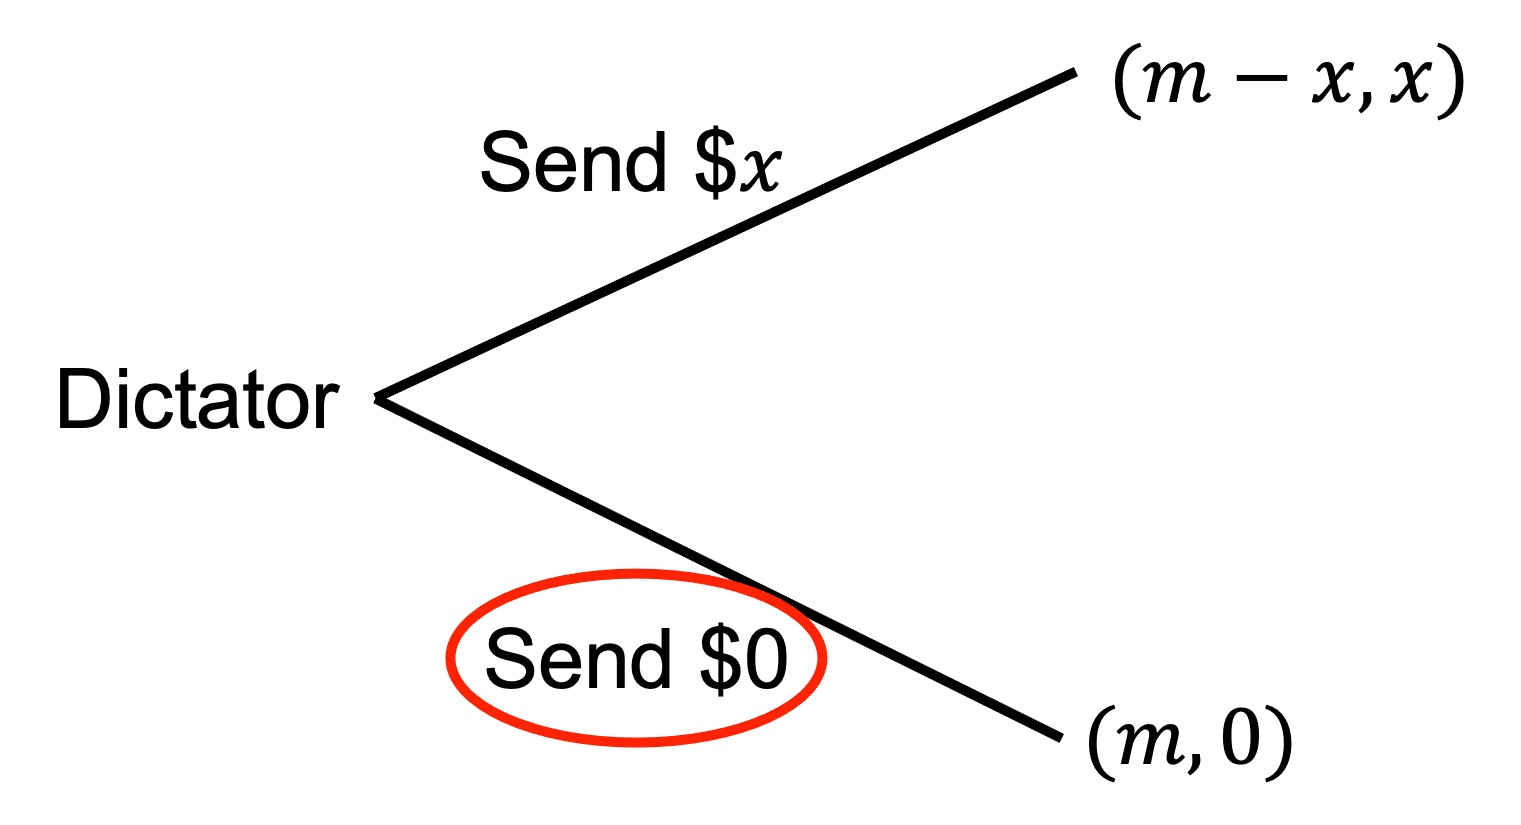
\includegraphics{game-theory/img/dictator-game-2.jpg}

\hypertarget{the-trust-game}{%
\subsection{The trust game}\label{the-trust-game}}

The trust game involves two players: a sender and a receiver

Both the sender and receiver are given an initial sum \(m\).

The sender sends a share \(x\) of their \(m\) to the receiver (the
investment).

Before the investment is received by the receiver, it is multiplied by
some factor \(k\).

The receiver receives \(kx\).

The receiver then returns to the sender some share \(y\) of their total
allocation \(m+kx\).

The final outcome is (\(m-x+y\), \(m+kx-y\)).

Here is a numerical example.

Suppose the sender and receiver are given an initial sum of \$10.

The sender decides to send \$5 of their \$10 to the receiver (the
investment).

This is multiplied by a factor of 3. Therefore, the receiver receives
\$15 and now has \$25.

The receiver then returns to the sender \$7.50 of their \$25.

The final outcome is (\$10−5+7.50, \$10+15−7.50)=(\$12.50, \$17.50).

The extensive form of the game is as follows.

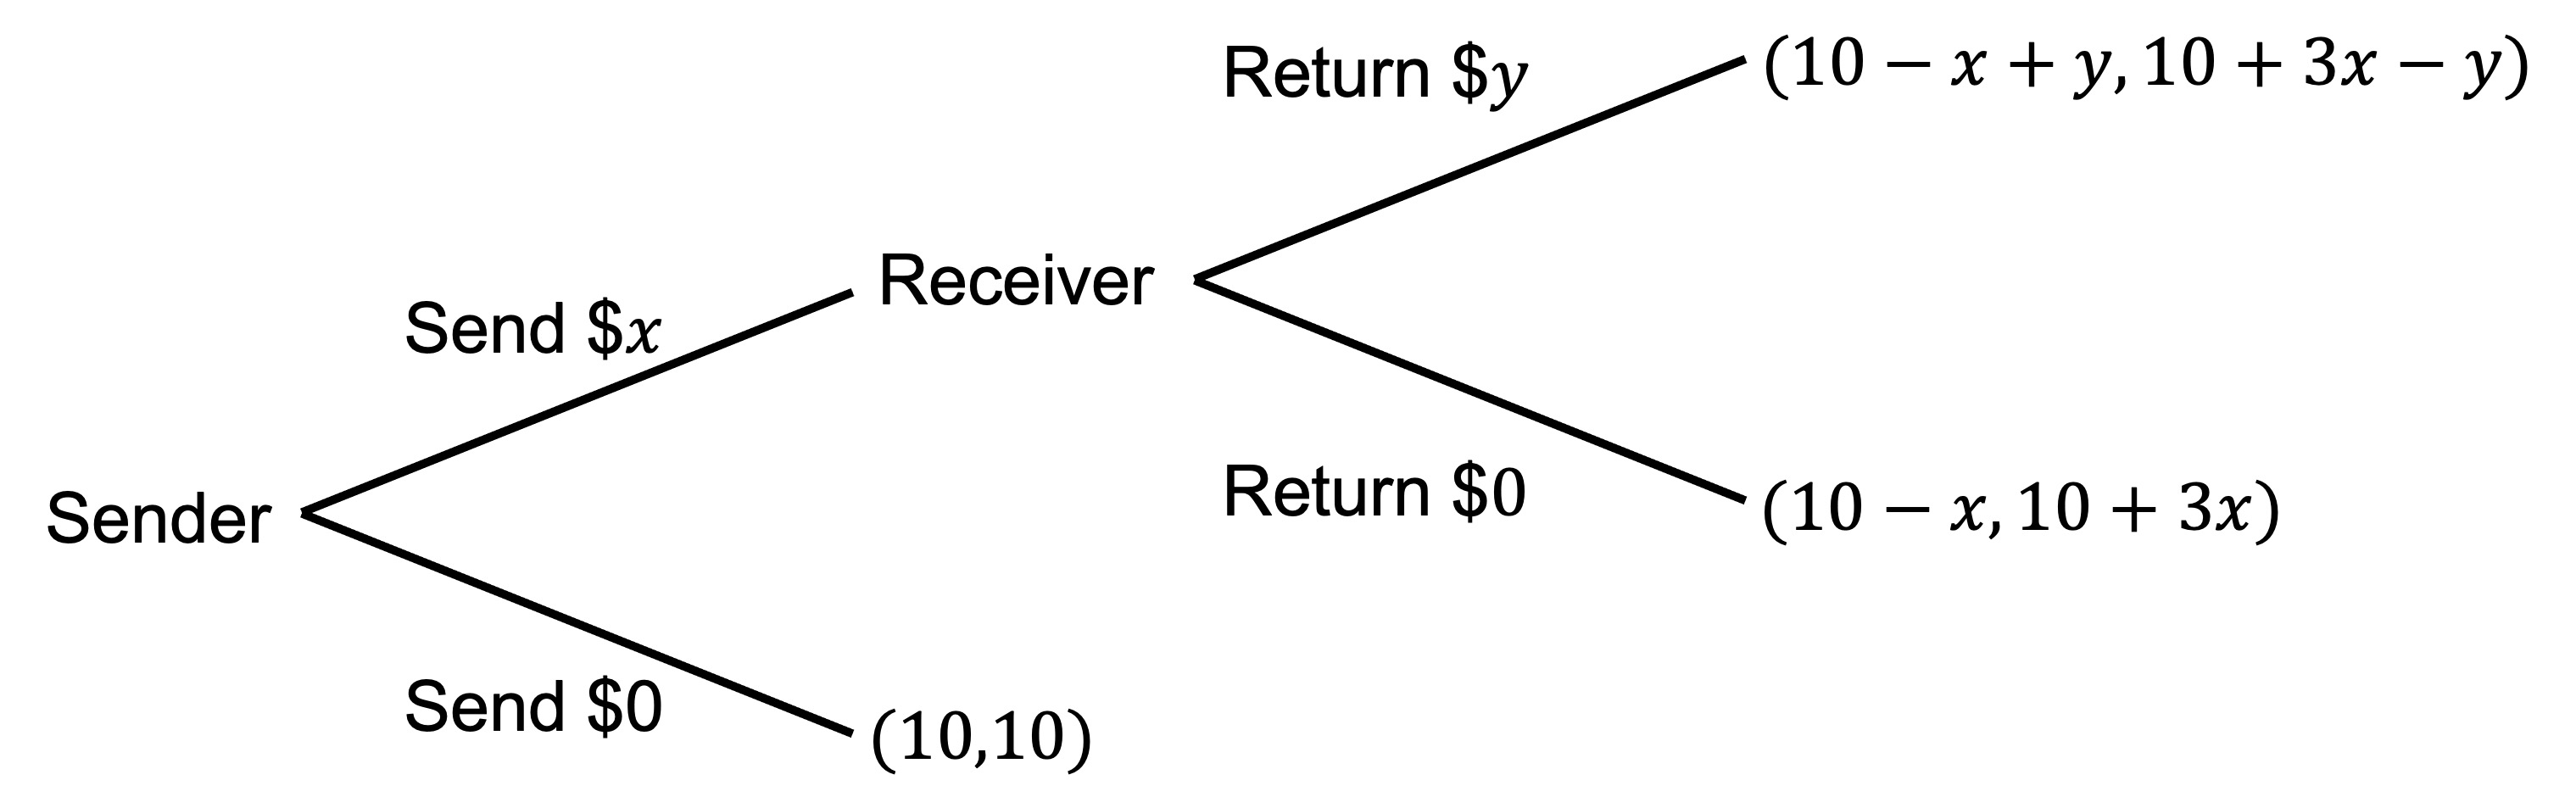
\includegraphics{game-theory/img/trust-game-1.jpg}

If both receivers have utility function \(u(x)=x\) the only
subgame-perfect equilibrium is that the receiver will keep all their
money, so the sender sends nothing.

One way to think about this problem is that the receiver is effectively
playing a dictator game.

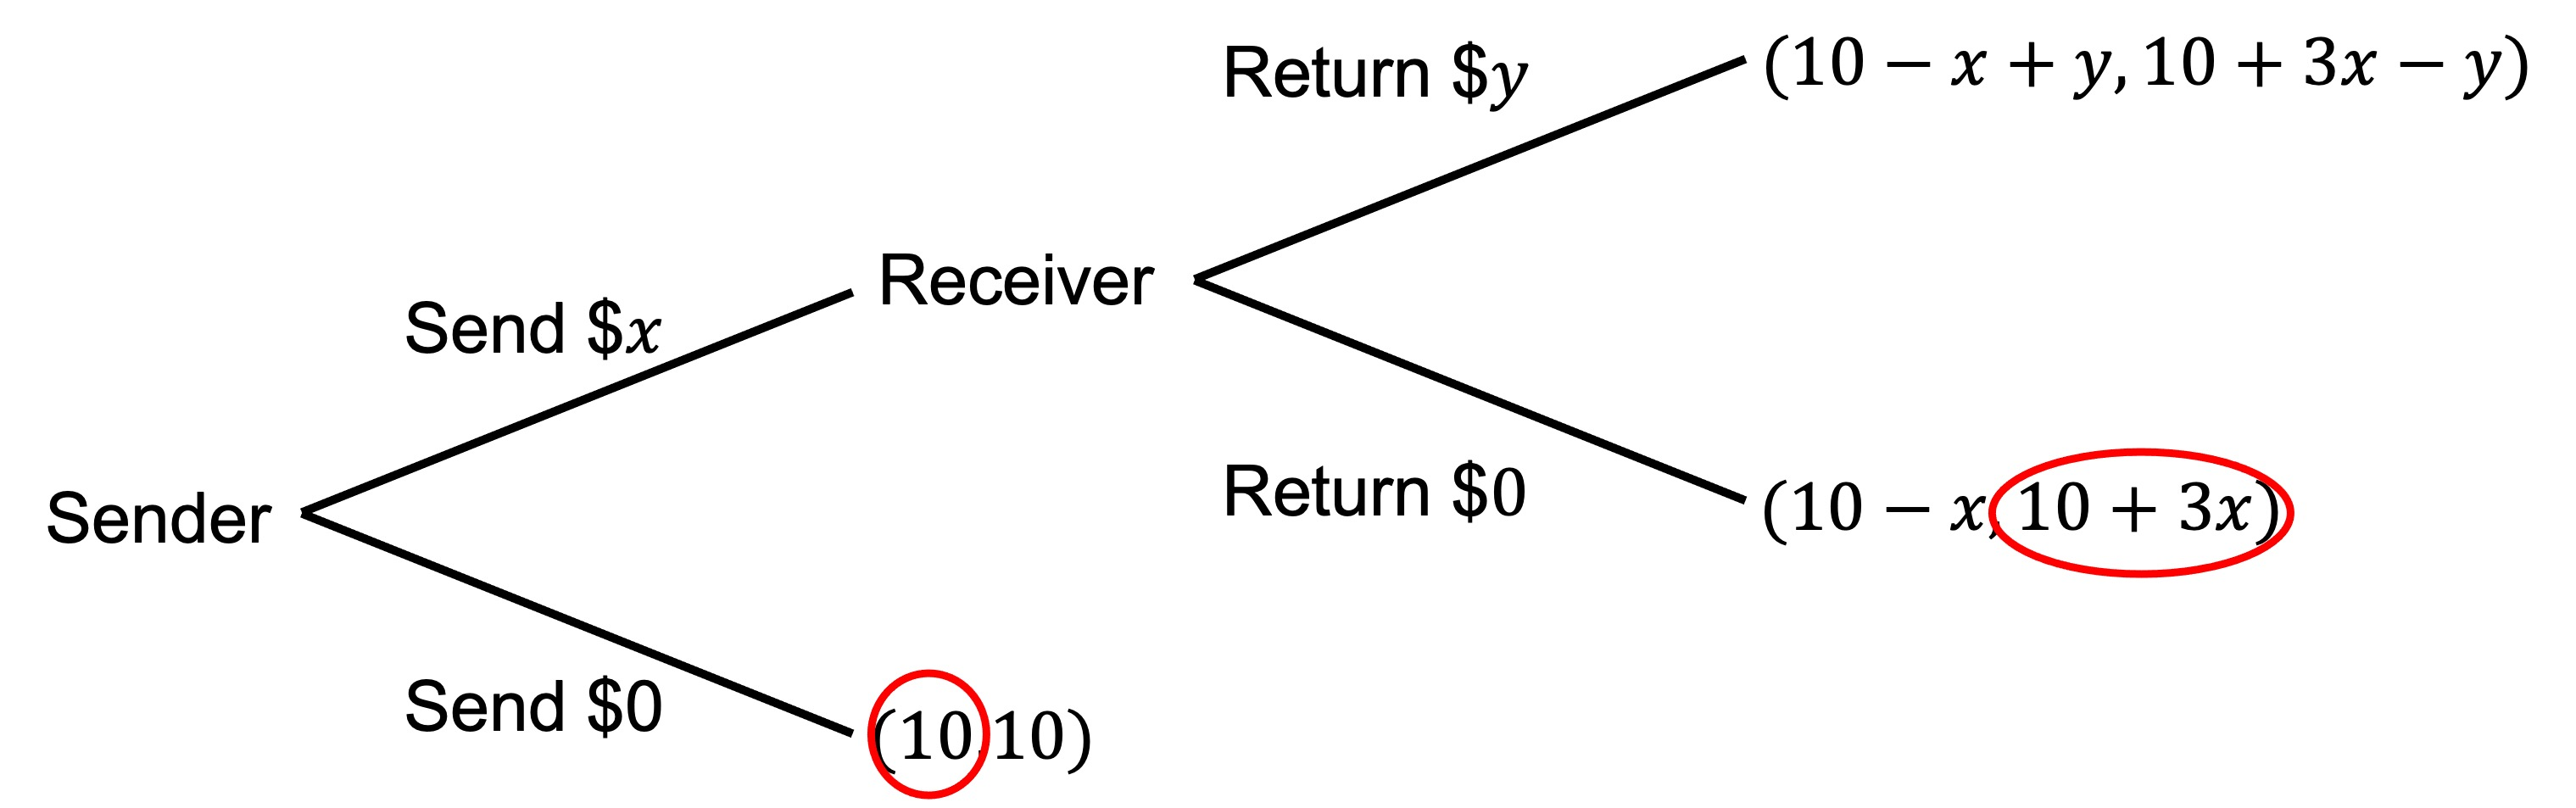
\includegraphics{game-theory/img/trust-game-2.jpg}

Relative to the Pareto optimal outcome whereby the sender's full
endowment is tripled and they receive a positive return on their
investment, both players are worse off under the equilibrium outcome.

\hypertarget{asymmetric-information}{%
\chapter{Asymmetric information}\label{asymmetric-information}}

To date we have assumed perfect information. That is, all players know
the rules of the game, the available actions and the payoffs from each
set of actions.

I will now explore two examples where we relax this assumption and allow
the parties to have different information. However, we will retain the
assumption of rational behaviour.

\hypertarget{the-market-for-lemons}{%
\section{The market for lemons}\label{the-market-for-lemons}}

This example draws on the work of Akerlof (1970)

An agent decides to buy a used car. Price \(p\) is fixed and quality is
unobservable.

Suppose there are two types of cars: good cars and lemons. A car is good
with probability \(q\) and a lemon with probability \(1−q\).

The seller knows the type. To the seller, good cars are worth \$10,000
and lemons \$5,000.

To potential buyers, good cars are worth \$15,000 and lemons \$7,500.

Before the purchase, the buyer knows the types of cars in the market and
the frequency of each. After the purchase, the buyer discovers the true
type.

Selling is the efficient solution as both car types worth more to buyers
than sellers. But what happens?

How much is a buyer willing to pay will depend on the proportion of good
cars and lemons offered for sale.

Let 𝜇 be the probability that a car that is sold is good. If sellers are
willing to sell their good cars, \(\mu=q\). If not, \(\mu=0\).

The expected value of a car to a buyer is:

\(E=\mu 15000+(1−\mu)7500=7500+\mu 7500\)

Hence, the buyer will be willing to pay up to \(p=7500+\mu 7500\).

Sellers will sell a lemon if 𝑝≥5000 and a good car if \(p≥10000\).

They will be able to sell the lemon if:

\[
5000≤p≤7500+\mu7500
\]

This always holds, so the seller will always be willing and able to sell
the lemon.

They will be able to sell the good car if:

\[
10000≤p≤7500+\mu7500
\]

This can only hold if \(\mu≥1/3\).

Assuming risk neutral buyers, there are two equilibria.

If \(q≥1/3\), sellers sell both types of cars:

\[
\mu=q≥1/3→10000≤p^∗≤7500+\mu7500
\]

If \(q<1/3\), sellers sell only lemons:

\[
𝜇=0→5000≤p^∗≤7500
\]

Generalising:

\begin{enumerate}
\def\labelenumi{\arabic{enumi}.}
\item
  When buyers cannot observe product quality, given 𝑝, sellers have an
  incentive to lower product quality. That is, sellers try to pass off
  lemons.
\item
  Rational buyers expect this seller behaviour and they lower their
  willingness to pay.
\item
  Prices decline.
\item
  Sellers lower quality further to make profits at the lower prices.
  Sellers cannot sell high quality cars at high prices even though
  buyers would be willing to pay the high prices for the high quality
  cars.
\item
  Quality declines until nothing but lemons are left.
\end{enumerate}

Information asymmetry is sufficient to result in a market failure even
if agents are rational.

\hypertarget{the-winners-curse}{%
\section{The winner's curse}\label{the-winners-curse}}

A common-value auction is an auction in which the item for sale has the
same value to all the bidders.

Examples include:

\begin{itemize}
\item
  Stocks, which all have one value, whatever traders' expectations
\item
  Oil, where the amount of oil in a tract is the same for all oil
  companies.
\end{itemize}

This contrasts with a private-value auction in which bidders have
different valuations for the item for sale. This typically occurs where
the item's valuation reflects bidder tastes, such as art.

The winner's curse is phenomenon in common value auctions whereby the
winner tends to experience a loss.

The term was invented by petroleum engineers in discussing why oil
companies in the Gulf of Mexico had mediocre results in the 1950−1970s.

Oil companies in the Gulf of Mexico acquired drilling rights through
auctions.

Their rights yielded losses or less in profits than expected. In
hindsight, the winning bids were unreasonably high.

The winner's curse is widely documented in experimental settings and has
been observed in corporate environments.

\hypertarget{winners-curse-example}{%
\subsection{Winner's curse example}\label{winners-curse-example}}

Company 1 and company 2 hire a geologist to estimate the value of an oil
field. The (truthful) geologist of company \(i\) privately reports their
estimated valuation \(v_i\) to company \(i\). Company 1 learns \(v_1\)
and company 2 learns \(v_2\).

\(v_1\) and \(v_2\) are uniformly distributed between \$0 and \$100 and
independent. Assume the true value of the oil field is the mean of
\(v_1\) and \(v_2\): \(\frac{v_1+v_2}{2}\)

The two companies simultaneously bid for the field. The highest bid wins
and pays their bid (first-price auction).

What should a company bid in this auction?

Suppose both companies bid the private valuation they receive. Company 1
receives \(v_1=50\), bids \$50 and wins.

\begin{itemize}
\item
  If they win, \(v_1=\$50>v_2\).
\item
  On average, in this state of the world company 2's signal is \$25 (due
  to uniform distribution). The average value of the tract is
  \((50+25)/2=\$37.50\).
\item
  Company 1 loses \$50 − \$37.50 = \$12.50 on average.
\end{itemize}

What if \(v_1=50\) and company 1 bids \$37.50 instead, company 2
continues to bid \(v_2\) and company 1 wins?

\begin{itemize}
\item
  If company 1 wins, \(\$37.50>v_2\).
\item
  On average, in this state of the world company 2's signal is \$18.75
  (due to uniform distribution). The average value of the tract is
  \((50 + 18.75)/2=\$34.37\).
\item
  Company 1's loses \$37.50− \$34.37=\$3.13 on average.
\end{itemize}

What if \(v_1=50\) and company 1 bids \$25 instead, company 2 continues
to bid \(v_2\) and company 1 wins?

\begin{itemize}
\item
  If company 1 wins, \(25>v_2\).
\item
  On average, in this state of the world company 2's signal is \$12.50
  (due to uniform distribution), so the average value of the tract is
  \((50 +12.50)/2=\$31.25\).
\item
  Company 1's profit is \$31.25 − \$25 = \$6.25 on average. However,
  they will win only 25\% of the time.
\end{itemize}

What if company 1 bids \(\delta v_1\), company 2 continues to bid
\(v_2\) and company 1 wins?

\begin{itemize}
\item
  If they win, \(\delta v_1>v_2\).
\item
  On average, in this state of the world company 2's signal is
  \(0.5\delta v_1\) (due to uniform distribution). The average value of
  the tract is therefore \((v_1+0.5\delta v_1 )∕2=(0.5+0.25\delta)v_1\).
\item
  Company 1's net profit on average is
  \(\pi=(0.5+0.25\delta)v_1−\delta v_1=(0.5−0.75\delta)v_1\). They make
  a profit where \(0.5−0.75\delta>0\), i.e.~where \(\delta<2/3\).
\item
  The lower \(\delta\) the higher their profit, but that is conditional
  on company 1 having the winning bid, which decreases in probability as
  they decrease \(\delta\).
\end{itemize}

This analysis has a complication in that it does not account for the
fact that company 2 is also a strategic player. We assumed company bids
\(v_2\), but as for company 1, this would strategy lead to an expected
loss for company 2.

For example, what if company 1 bids \(x=\delta v_1=2/3v_1\), company 2
bids \(v_2\) and company 2 wins?

\begin{itemize}
\item
  If they win, \(x=\delta v_1<v_2\).
\item
  On average, in this state of the world company 1's bid is \(0.5v_2\)
  (due to uniform distribution) and company 1's signal
  \(\frac{0.5v_2}{2/3}=3/4v_2\). The average value of the tract is
  therefore \((\frac{3}{4}v_2+v_2 )/2=0.875v_2\).
\item
  Company 2's net profit on average is \(\pi=0.875v_2−v_2=−0.125v_2\).
\end{itemize}

What does each firm do at equilibrium?

As each firm will have the same strategy at equilibrium, we can solve
for company 1 assuming company 2 does the same strategy in response. At
equilibrium we can also assume that each company will have an expected
profit of zero as each company would otherwise have an incentive to
change their bid to gain a share of that profit.

Company 1 will win if \(\delta v_1>\delta v_2\); i.e.~if \(v_1>v_2\). On
average, in this state of the world company 2's signal is \(0.5v_1\)
(due to uniform distribution), so that the average value of the tract is
\((v_1+0.5v_1)/2=0.75v_1\).

Company 1's profit is:

\[
\pi_1=(v_1+v_2)/2−\delta𝑣_1=(0.75−\delta)v_1
\]

Profit is zero when \(\delta=0.75\). The Nash equilibrium is that both
parties bid 75\% of their private valuation.

In summary, bidding based purely on your own valuation fails to take
into account that you only win if player 2's signal is low.

Alternatively, we may say that winning the auction is bad news regarding
the value of the field. This is the winner's curse.

Because of the winner's curse, the Nash equilibrium is to bid more
conservatively.

The mistake oil companies is to ignore or underestimate the winner's
curse.

If an oil company wins an auction, it's likely in part because its
geologists have the highest estimates of the field's value. But if all
other geologists have lower estimates of the value, the company's
geologists have probably overestimated it.

\hypertarget{strategic-moves-and-commitment}{%
\chapter{Strategic moves and
commitment}\label{strategic-moves-and-commitment}}

\hypertarget{chicken}{%
\section{Chicken}\label{chicken}}

Consider the following game of chicken. Two players are driving toward
each other. Whoever swerves first loses. If neither swerves, they crash
and die.

\includegraphics{game-theory/img/chicken-1.jpg}

There are two pure-strategy Nash equilibria: (Straight, Swerve) and
(Swerve, Straight). If the other player swerves, they want to go
straight. If the other player goes straight, they want to swerve.

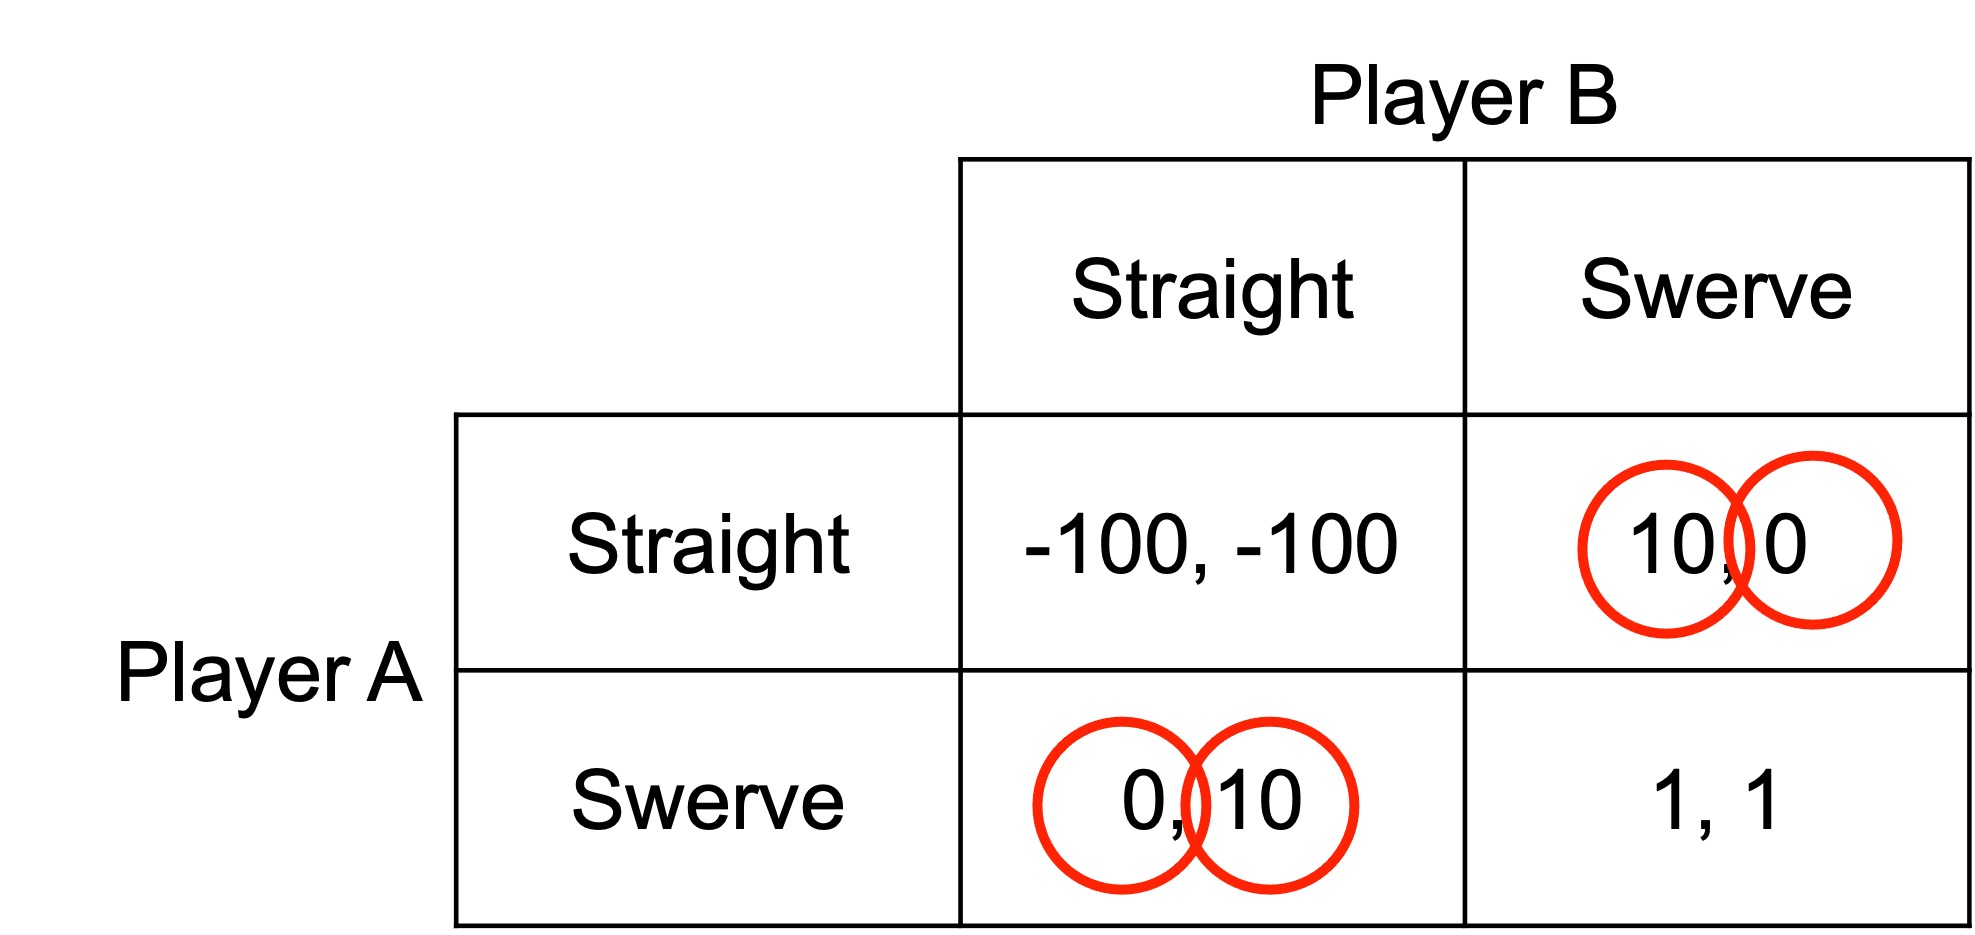
\includegraphics{game-theory/img/chicken-2.jpg}

As they are driving toward each other, Player A rips the steering wheel
out of their car and throws it out the window. They will now drive
straight no matter what Player B does.

\includegraphics{game-theory/img/chicken-3.jpg}

This is effectively a new game. What is the Nash equilibrium?

The Nash equilibrium is (Straight, Swerve). Player A wins the game of
chicken.

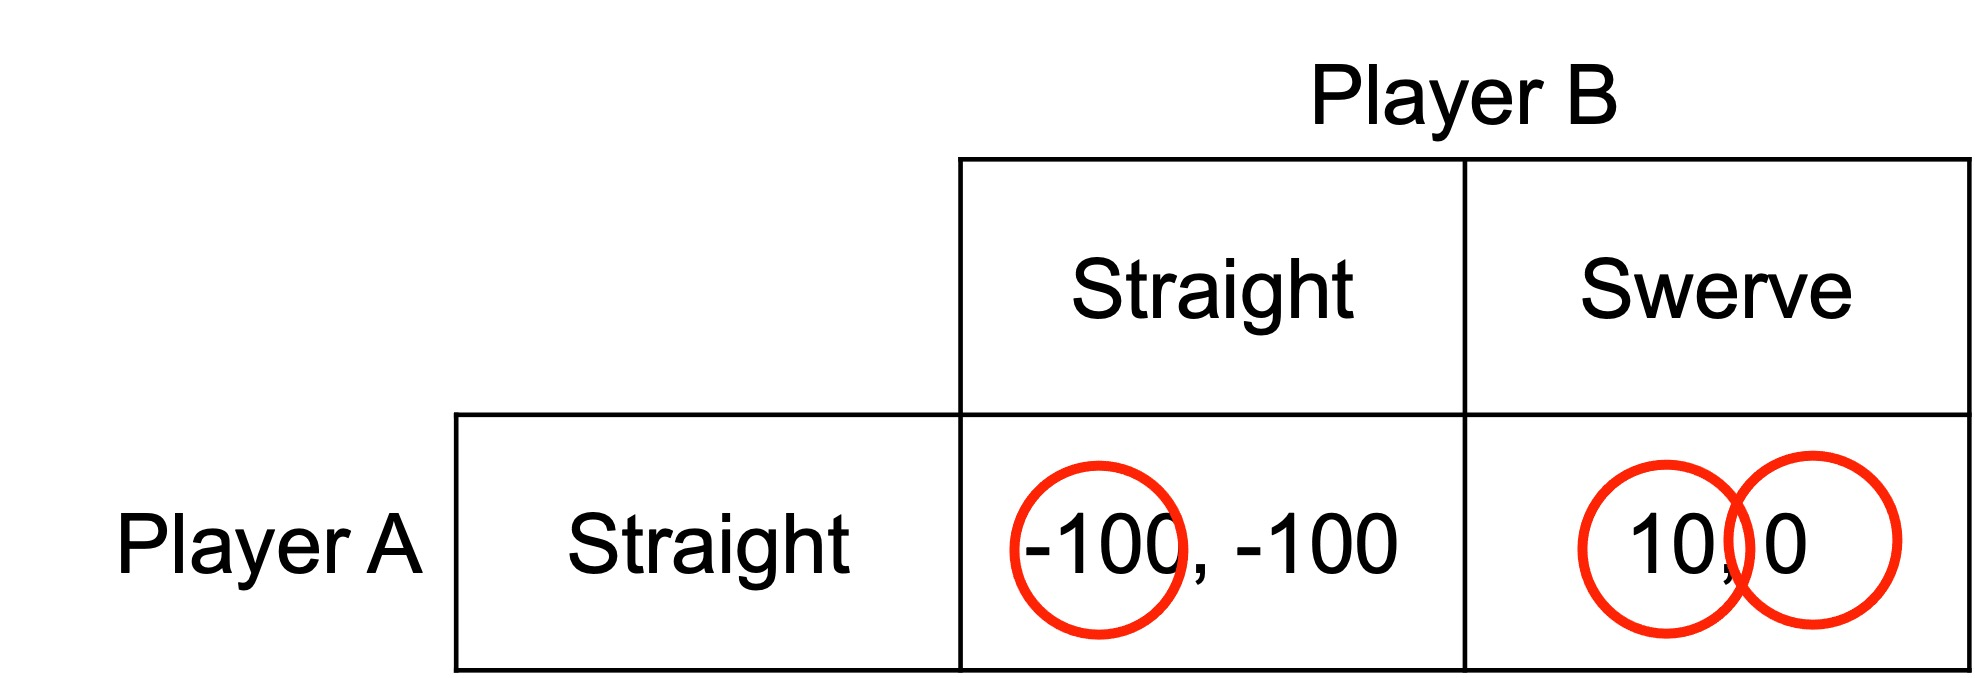
\includegraphics{game-theory/img/chicken-4.jpg}

\hypertarget{strategic-moves}{%
\section{Strategic moves}\label{strategic-moves}}

The option to commit to a course of action as in this game of chicken is
an example of a strategic move.

A strategic move changes the game you are playing from a single-stage
game to a two-stage game. In the first stage you make your strategic
move. In the second you play the original game.

Strategic moves come in two forms:

\begin{itemize}
\item
  Unconditional: commitments
\item
  Conditional: threats and promises
\end{itemize}

\hypertarget{unconditional-strategic-moves}{%
\section{Unconditional strategic
moves}\label{unconditional-strategic-moves}}

An unconditional strategic move is a commitment. For example, removing
your steering wheel in chicken is a commitment.

The commitment needs to be:

\begin{itemize}
\item
  Observable: your opponent should be able to observe your commitment.
  Otherwise you can claim to have made the commitment when you have not.
\item
  Irreversible: you cannot undo your commitment. Otherwise, the game
  remains as if you had never made it.
\end{itemize}

\hypertarget{conditional-strategic-moves}{%
\section{Conditional strategic
moves}\label{conditional-strategic-moves}}

A conditional strategic move involves specifying to your opponent how
you will respond to each move.

\begin{itemize}
\item
  Threats: ''If you don't clean your room, you won't get dessert.''
\item
  Promises: ``If you clean you room, you can have dessert.''
\end{itemize}

\hypertarget{credibility-of-strategic-moves}{%
\section{Credibility of strategic
moves}\label{credibility-of-strategic-moves}}

Commitments, threats and promises only achieve their objective if they
are credible. That is, they only work if the other player believes they
will be carried out as stated.

Sticking to a commitment and carrying out a threat or a promise
typically reduces the possible actions of the player.

If the proposer loses too much from carrying out a threat or promise,
they will not carry it out.

\hypertarget{example-4}{%
\subsection{Example}\label{example-4}}

You threaten to complain about a poor service by a company. Complaining
is costly.

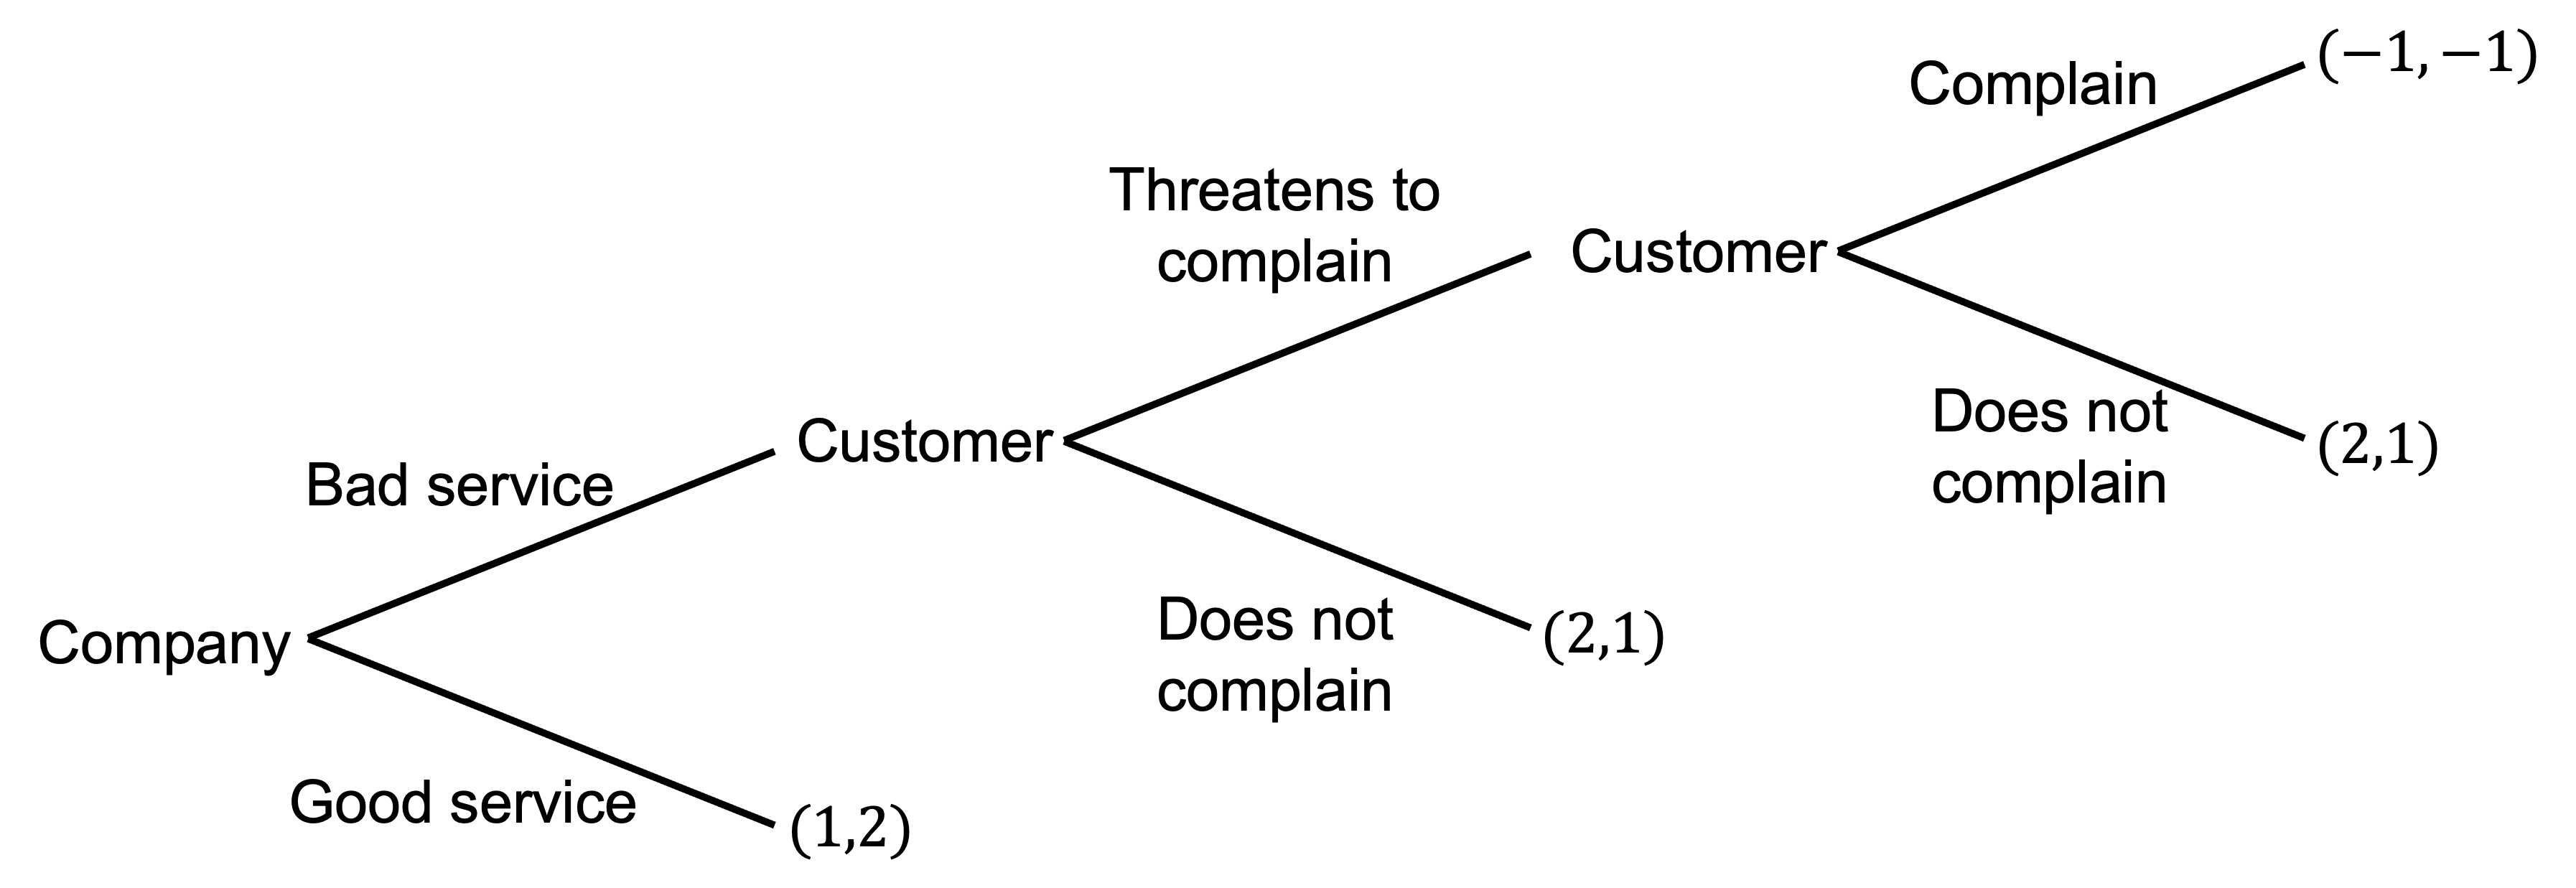
\includegraphics{game-theory/img/complain-1.jpg}

There are two sub-game perfect Nash equilibria: (Threatens to complain,
Bad service, Does not complain) and (No threat, Bad service). The threat
to complain is not credible.

\includegraphics{game-theory/img/complain-2.jpg}

\hypertarget{game-theory-exercises}{%
\chapter{Game theory exercises}\label{game-theory-exercises}}

\hypertarget{the-cold-war}{%
\section{The cold war}\label{the-cold-war}}

The year is 1964 and the Soviet Union and the United States are in the
midst of the cold war.

Suppose each player is considering whether they should act aggressively
(hawk) or peacefully (dove). If one plays hawk while the other plays
dove, they win the cold war. If both play hawk, there is a nuclear
armageddon.

The payoffs (\(x,y\)) of each option for the Soviet Union and United
States is as follows:

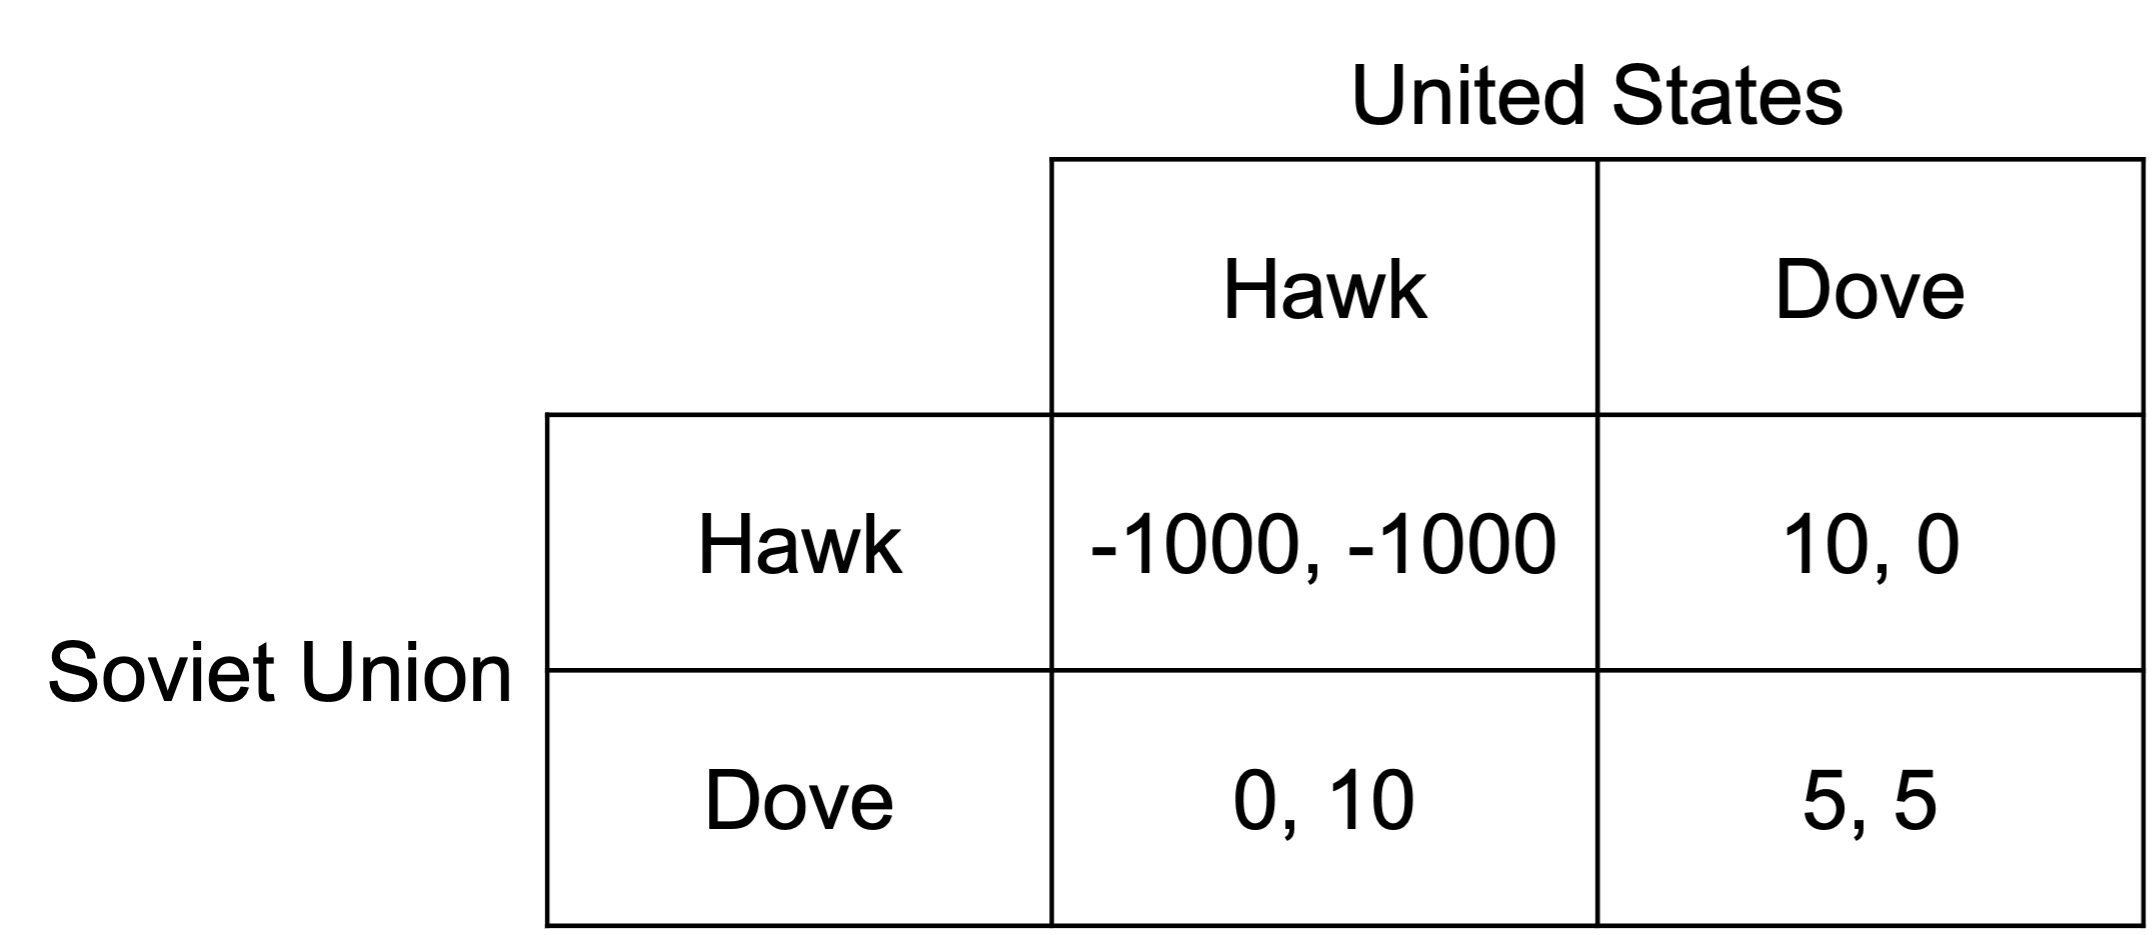
\includegraphics{game-theory/img/hawk-dove-1.jpg}

a) What is the Nash equilibrium of this game? What other game does this
resemble?

\begin{tcolorbox}[enhanced jigsaw, title=\textcolor{quarto-callout-tip-color}{\faLightbulb}\hspace{0.5em}{Answer}, toprule=.15mm, colback=white, breakable, titlerule=0mm, colframe=quarto-callout-tip-color-frame, coltitle=black, opacityback=0, rightrule=.15mm, colbacktitle=quarto-callout-tip-color!10!white, bottomtitle=1mm, opacitybacktitle=0.6, arc=.35mm, bottomrule=.15mm, toptitle=1mm, leftrule=.75mm, left=2mm]

The preferred action in response to the action of the other player are
indicated in the below diagram.

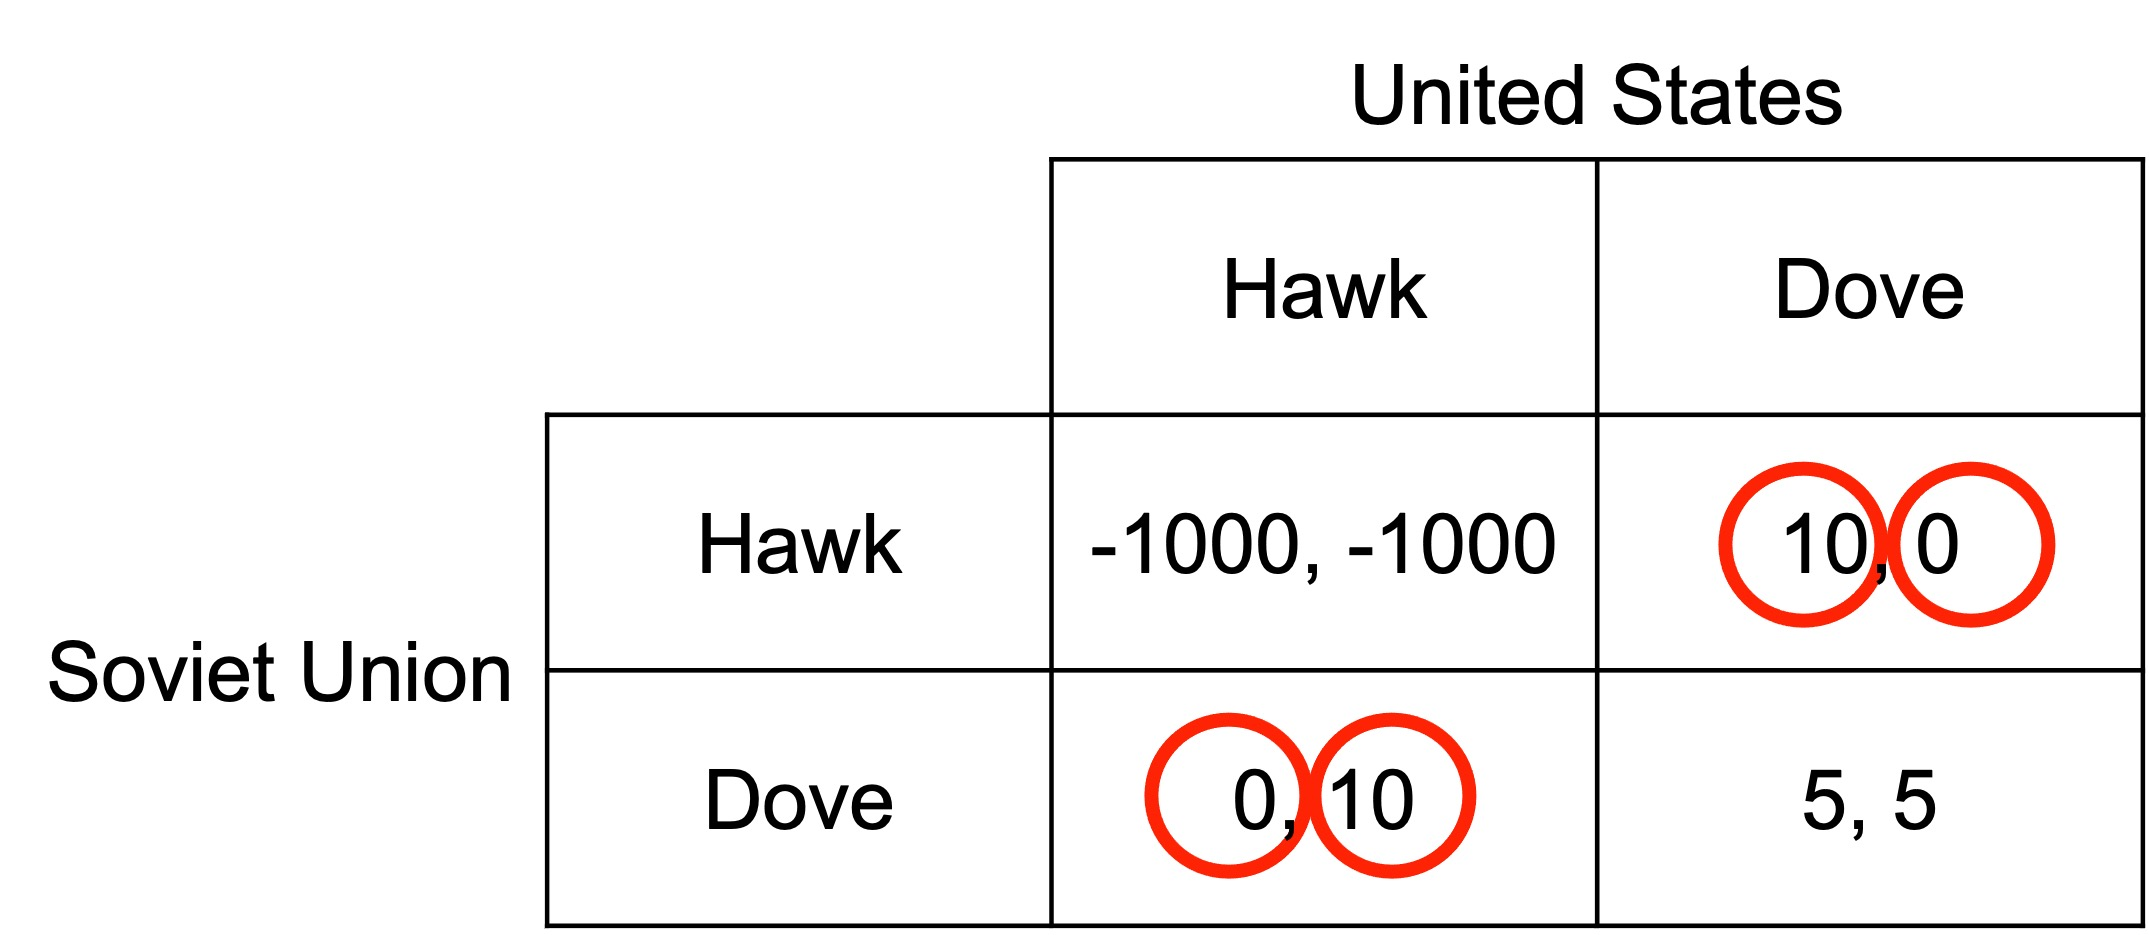
\includegraphics{game-theory/img/hawk-dove-2.jpg}

The two Nash equilibria are (Hawk, Dove) and (Dove, Hawk).

This game resembles chicken. Each player wants to win, but if neither
swerve, there is a catastrophic outcome for both.

\end{tcolorbox}

b) In the movie Dr Strangelove, the Soviet Union created a doomsday
machine that would detonate automatically if there was a nuclear strike.
The fallout would render the earth uninhabitable. The doomsday machine
could not be deactivated and would explode if any attempt was made.

Explain how the doomsday device could act as a commitment device?

\begin{tcolorbox}[enhanced jigsaw, title=\textcolor{quarto-callout-tip-color}{\faLightbulb}\hspace{0.5em}{Answer}, toprule=.15mm, colback=white, breakable, titlerule=0mm, colframe=quarto-callout-tip-color-frame, coltitle=black, opacityback=0, rightrule=.15mm, colbacktitle=quarto-callout-tip-color!10!white, bottomtitle=1mm, opacitybacktitle=0.6, arc=.35mm, bottomrule=.15mm, toptitle=1mm, leftrule=.75mm, left=2mm]

By removing dove as a response to hawk, the game effectively changes to
the following:

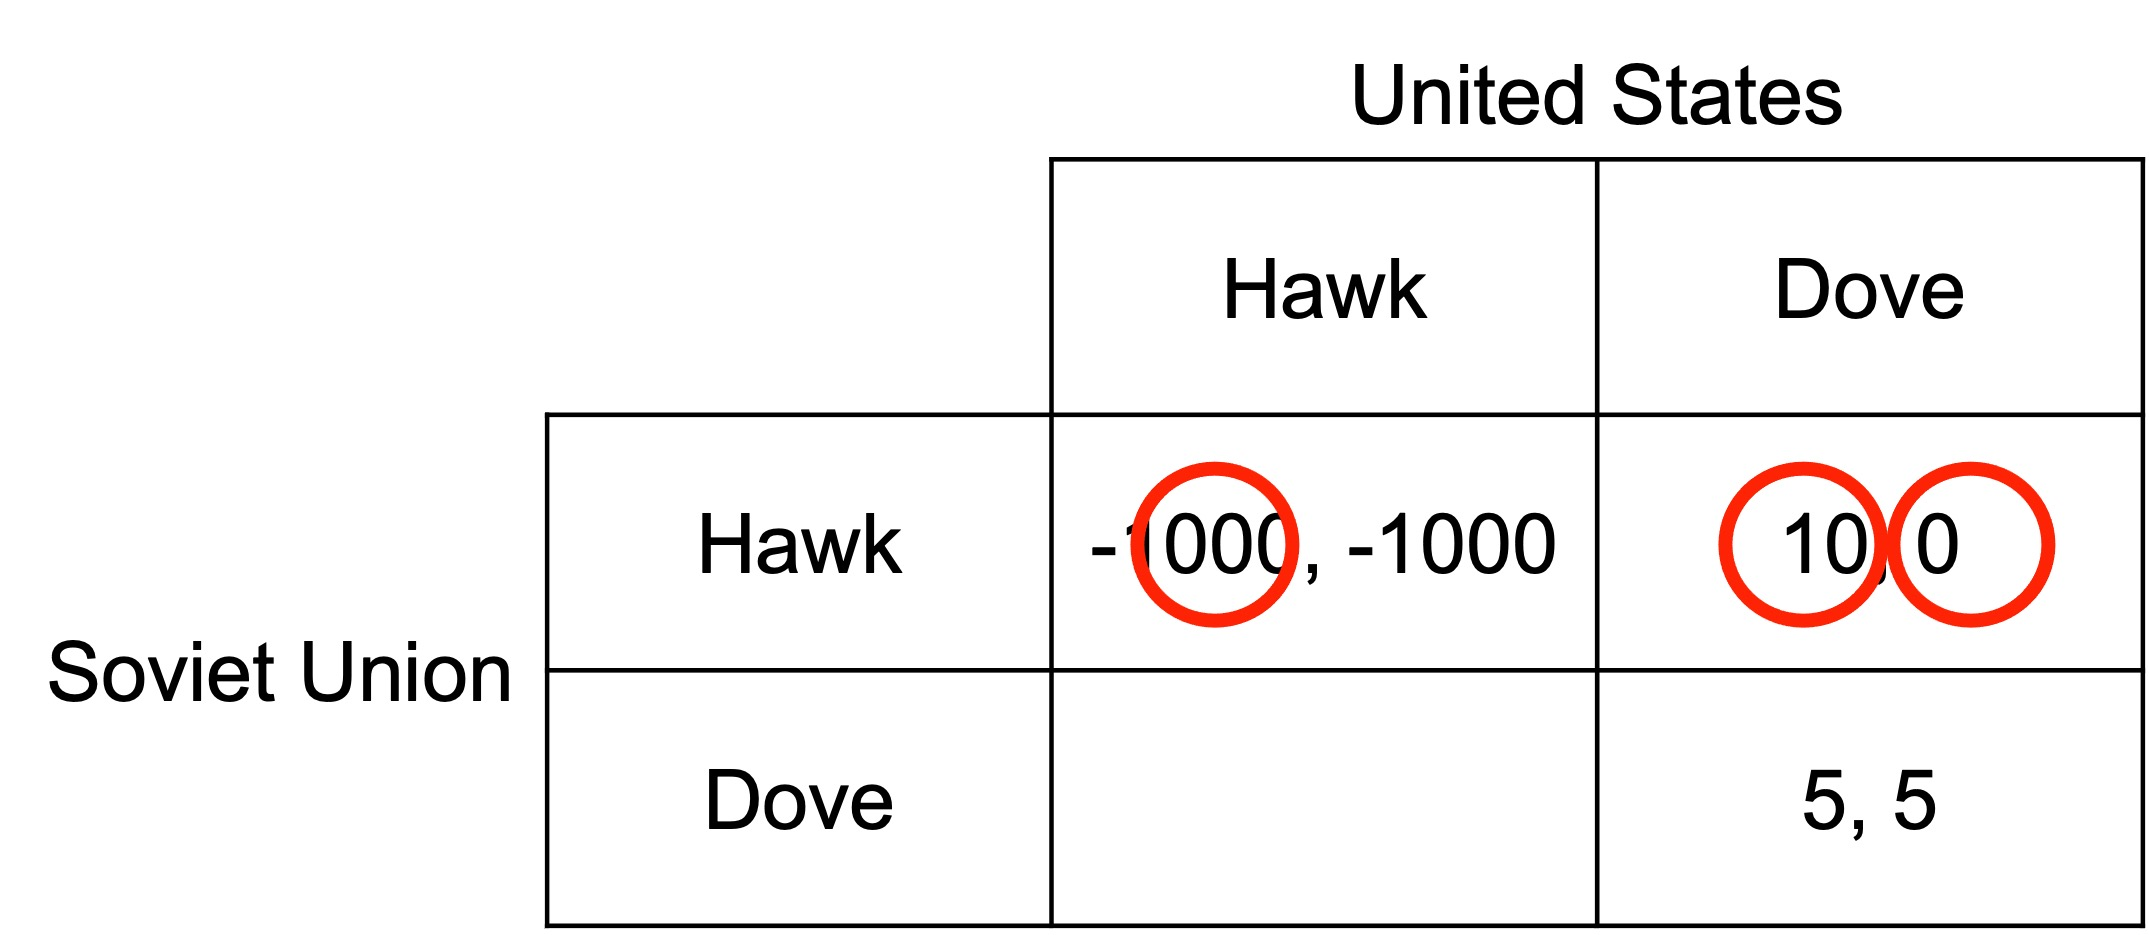
\includegraphics{game-theory/img/hawk-dove-3.jpg}

The Soviet Union can now credibly signal that it will respond to hawk
with hawk. This leads to a single Nash equilibrium: (Hawk, Dove).

\end{tcolorbox}

c) In the movie, the Soviet Union failed to inform the United States of
the existence of the device. How could this failure to inform undermine
its effectiveness as a commitment device?

\begin{tcolorbox}[enhanced jigsaw, title=\textcolor{quarto-callout-tip-color}{\faLightbulb}\hspace{0.5em}{Answer}, toprule=.15mm, colback=white, breakable, titlerule=0mm, colframe=quarto-callout-tip-color-frame, coltitle=black, opacityback=0, rightrule=.15mm, colbacktitle=quarto-callout-tip-color!10!white, bottomtitle=1mm, opacitybacktitle=0.6, arc=.35mm, bottomrule=.15mm, toptitle=1mm, leftrule=.75mm, left=2mm]

A commitment will only be effective if it is both observable and
irreversible. While the doomsday machine is irreversible, by not being
observable it will not change the response of the United States. The
United States will think they are playing the game analysed in part a),
not that in part b).

\end{tcolorbox}

\hypertarget{hiring}{%
\section{Hiring}\label{hiring}}

Robyn is hunting for a new employee. Robyn's company uses
highly-technical equipment and needs to invest heavily in training the
new employee. If the new employee leaves straight after training,
Robyn's company will suffer a net loss from the employee. If the
employee stays long-term, they will have a large gain.

Robyn approaches Sean and asks if he is interested in a long-term role
with the company.

Sean is interested in the training as he could use it to boost his
career, but sees less benefit in staying long-term. He considers whether
he should say he is interested or not.

The extensive form of the game is laid out below, with the payoffs
(\(x,y\)) being for Robyn and Sean respectively.

a) Will Robyn offer the position to Sean?

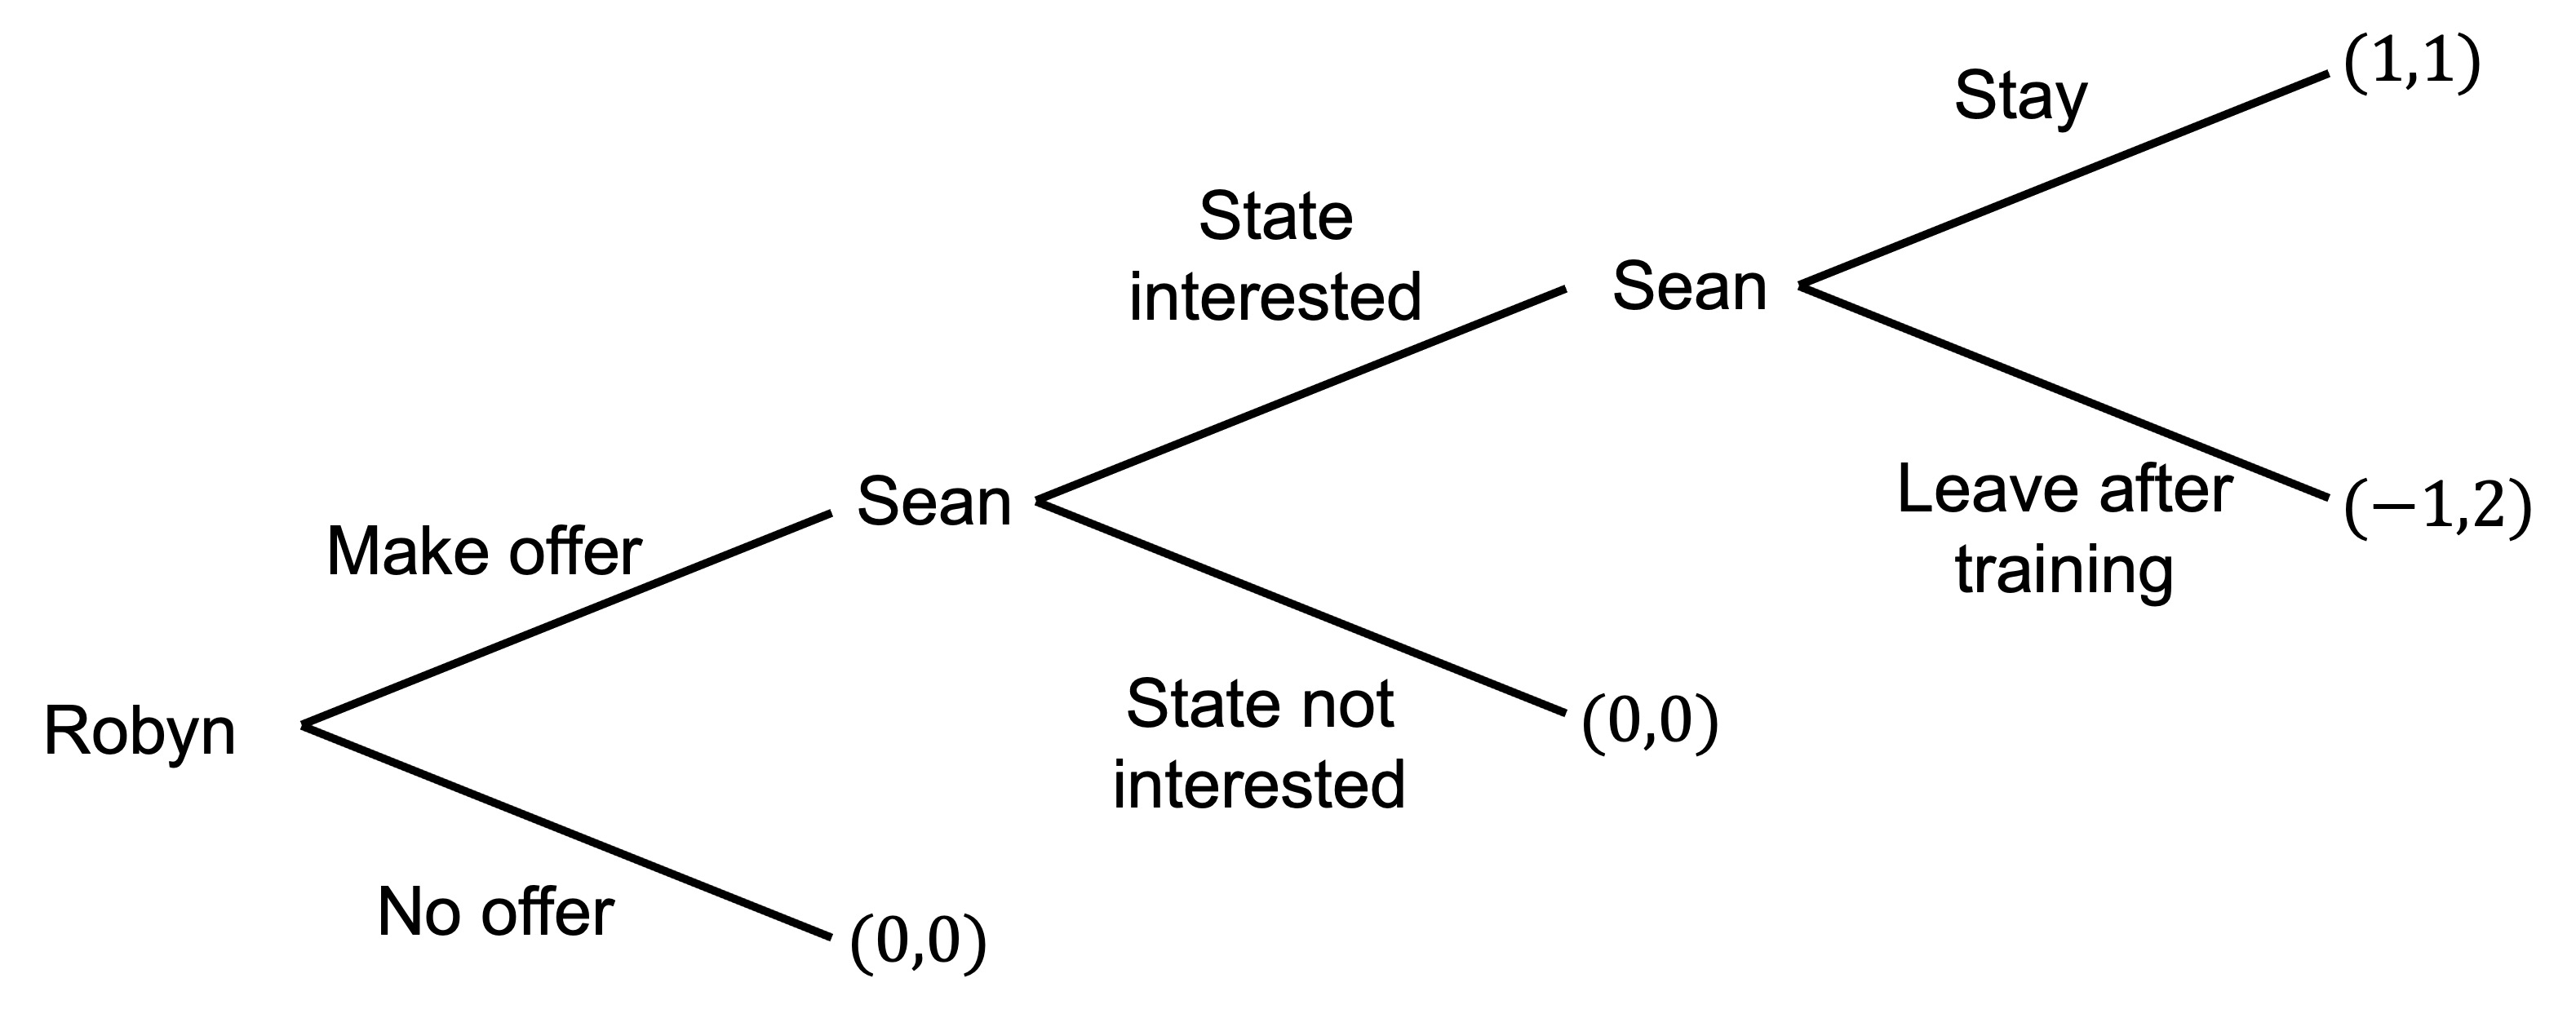
\includegraphics{game-theory/img/employment-1.jpg}

\begin{tcolorbox}[enhanced jigsaw, title=\textcolor{quarto-callout-tip-color}{\faLightbulb}\hspace{0.5em}{Answer}, toprule=.15mm, colback=white, breakable, titlerule=0mm, colframe=quarto-callout-tip-color-frame, coltitle=black, opacityback=0, rightrule=.15mm, colbacktitle=quarto-callout-tip-color!10!white, bottomtitle=1mm, opacitybacktitle=0.6, arc=.35mm, bottomrule=.15mm, toptitle=1mm, leftrule=.75mm, left=2mm]

We work through the problem by backward induction.

Sean can get 2 by leaving after training or 1 by staying. He leaves
after training.

When considering whether he will state that he is interested, he could
get 2 for stating he is interested (as he will later leave) versus
nothing for saying he is not interested. He states he is interested.

Robyn compares the -1 she gets for hiring Sean (as he will leave) with
the zero for no offer. She does not make an offer.

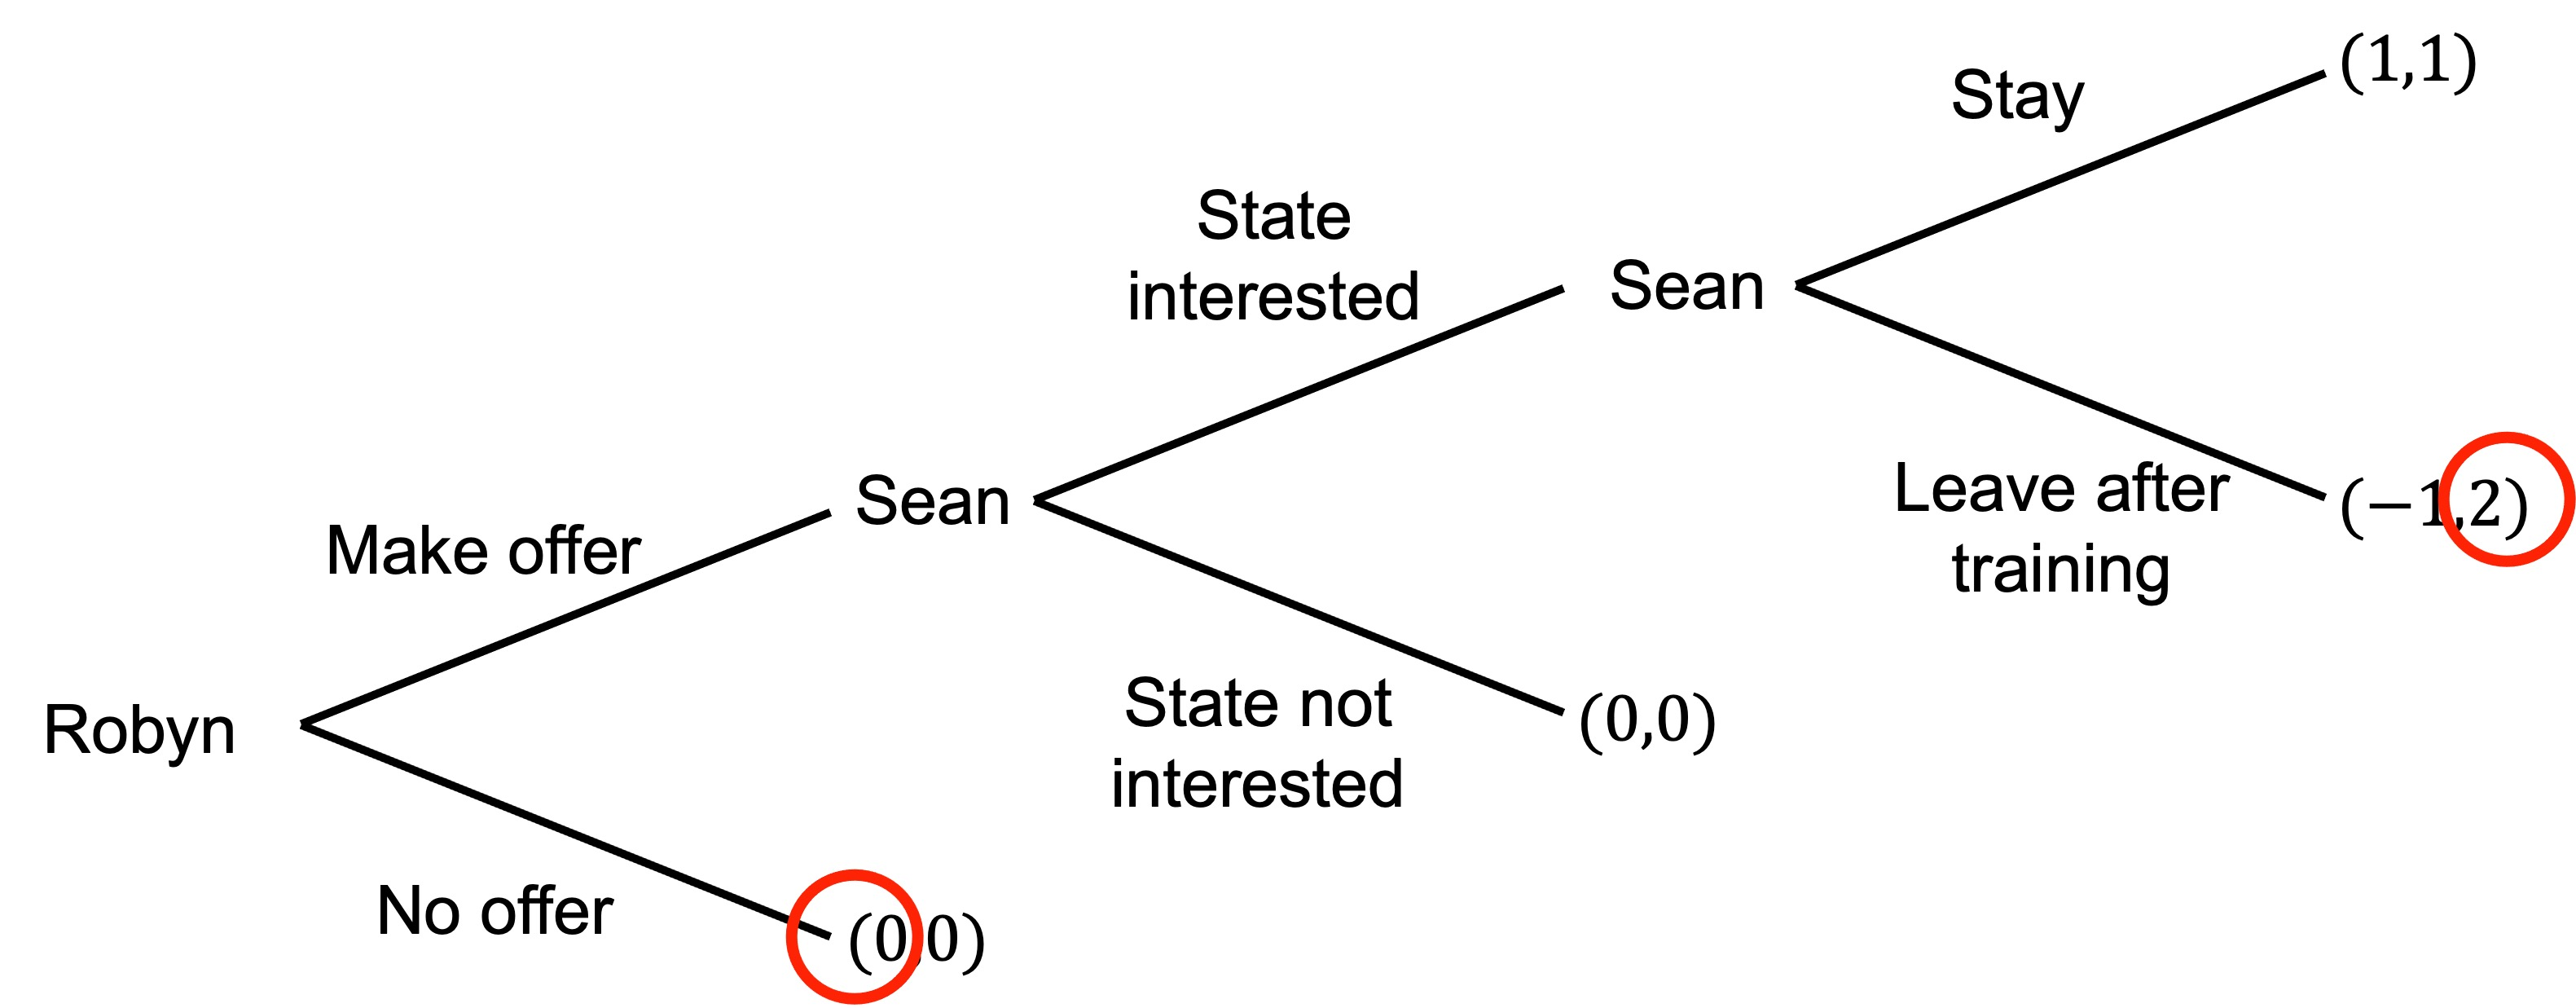
\includegraphics{game-theory/img/employment-2.jpg}

The subgame-perfect equilibrium is (No offer; State interested, Leave
after training).

\end{tcolorbox}

b) What sort of strategic move could help John? What could make the move
credible?

\begin{tcolorbox}[enhanced jigsaw, title=\textcolor{quarto-callout-tip-color}{\faLightbulb}\hspace{0.5em}{Answer}, toprule=.15mm, colback=white, breakable, titlerule=0mm, colframe=quarto-callout-tip-color-frame, coltitle=black, opacityback=0, rightrule=.15mm, colbacktitle=quarto-callout-tip-color!10!white, bottomtitle=1mm, opacitybacktitle=0.6, arc=.35mm, bottomrule=.15mm, toptitle=1mm, leftrule=.75mm, left=2mm]

One option is to sign a binding contract with penalties if he leaves
early. Any penalty greater than -1 would make staying more attractive.

A contract is both observable and irreversible (at least without mutual
agreement).

\end{tcolorbox}

\hypertarget{investment}{%
\section{Investment}\label{investment}}

Linda is looking for investment opportunities. She identifies a
promising crypto-based start-up created by an Marco. Marco is looking
for seed funding.

Linda can invest \$10.

If Linda invests, her investment will triple in value. Marco can then
decide to either shut down the start-up and keep the \$30 or maintain
the start-up in the market and pay a \$15 dividend to each of Linda and
himself.

If Linda does not invest, Linda keeps the \$10. The start-up gets \$0.

a) Draw the extensive form representation of the above sequential game.

\begin{tcolorbox}[enhanced jigsaw, title=\textcolor{quarto-callout-tip-color}{\faLightbulb}\hspace{0.5em}{Answer}, toprule=.15mm, colback=white, breakable, titlerule=0mm, colframe=quarto-callout-tip-color-frame, coltitle=black, opacityback=0, rightrule=.15mm, colbacktitle=quarto-callout-tip-color!10!white, bottomtitle=1mm, opacitybacktitle=0.6, arc=.35mm, bottomrule=.15mm, toptitle=1mm, leftrule=.75mm, left=2mm]

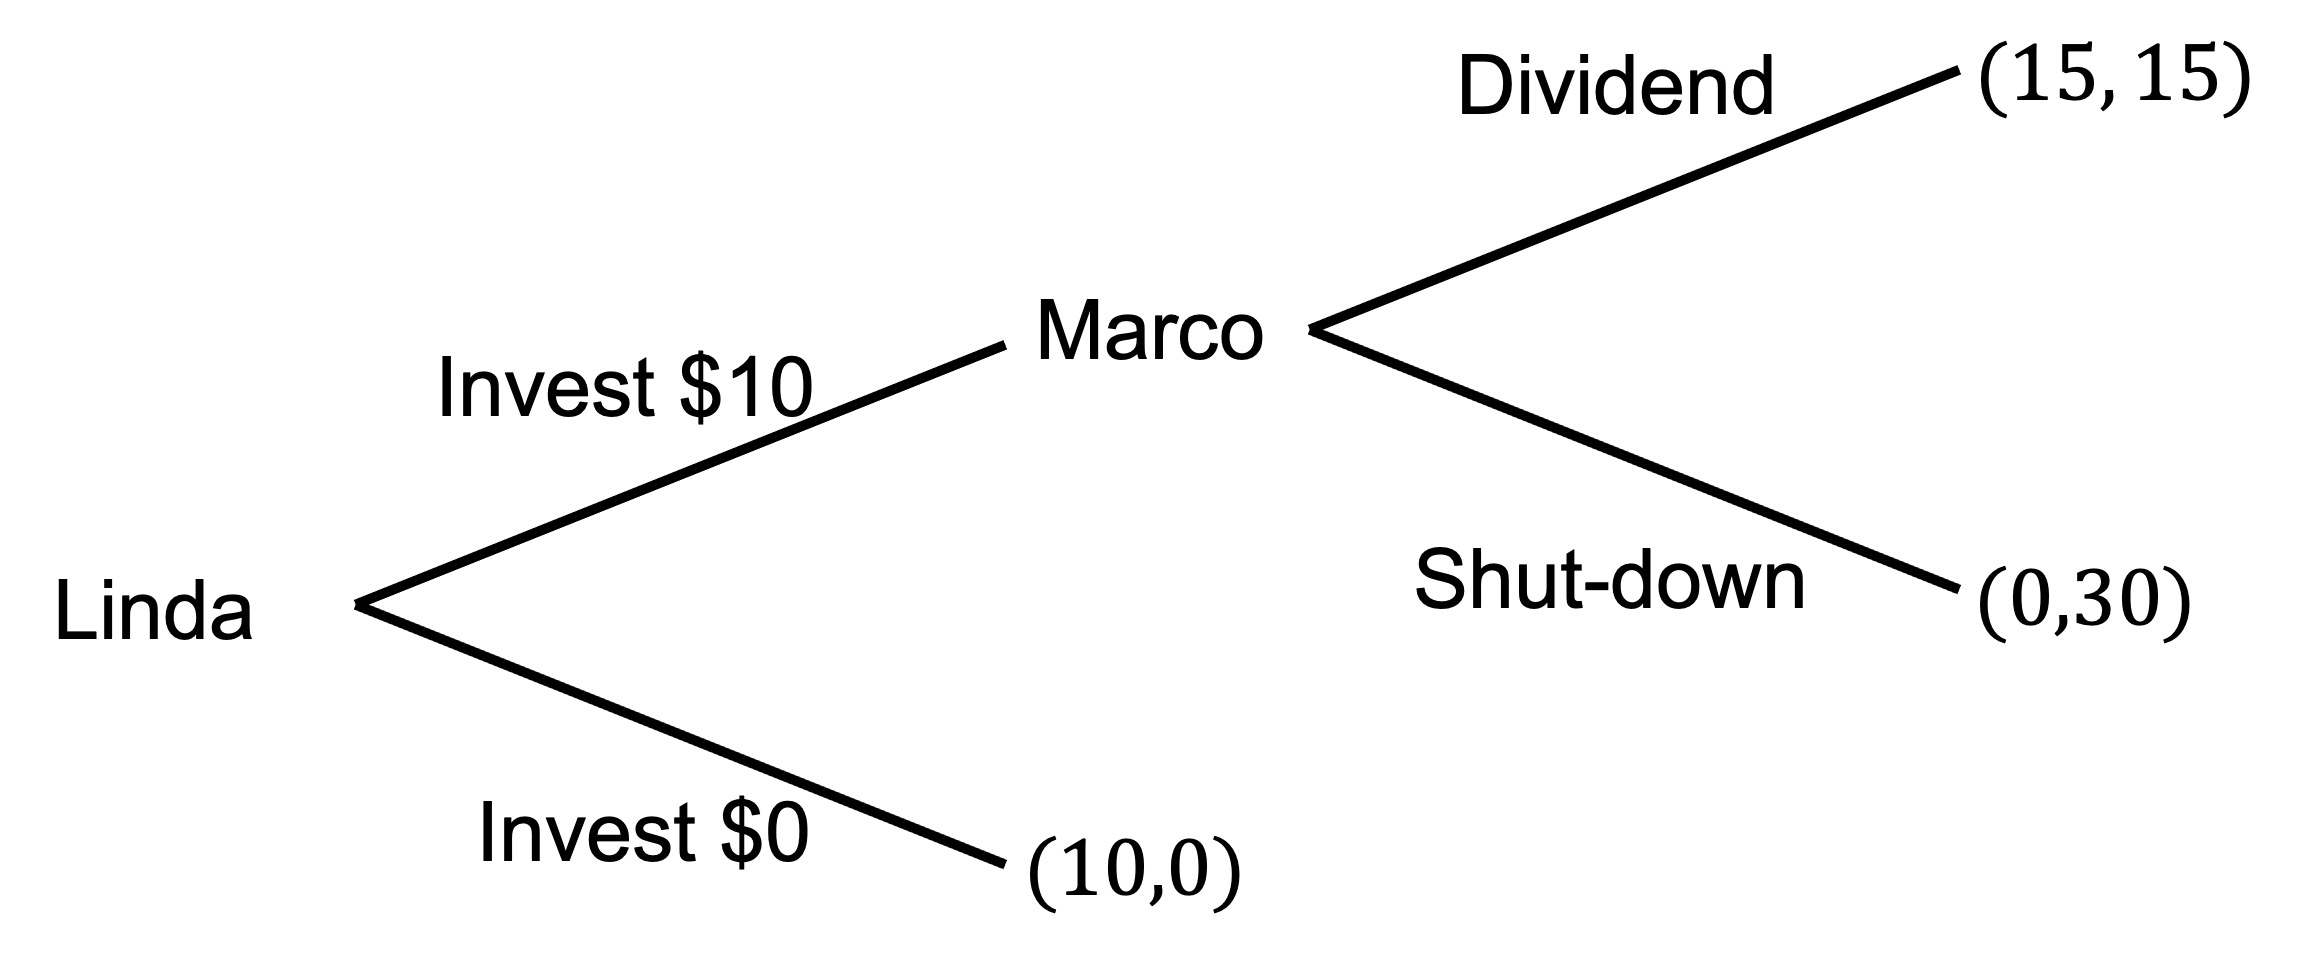
\includegraphics{game-theory/img/applied-trust-1.jpg}

\end{tcolorbox}

b) What is the equilibrium of this game if Linda and Marco are purely
self-interested?

\begin{tcolorbox}[enhanced jigsaw, title=\textcolor{quarto-callout-tip-color}{\faLightbulb}\hspace{0.5em}{Answer}, toprule=.15mm, colback=white, breakable, titlerule=0mm, colframe=quarto-callout-tip-color-frame, coltitle=black, opacityback=0, rightrule=.15mm, colbacktitle=quarto-callout-tip-color!10!white, bottomtitle=1mm, opacitybacktitle=0.6, arc=.35mm, bottomrule=.15mm, toptitle=1mm, leftrule=.75mm, left=2mm]

Marco will shutdown (payoff 30 versus payoff of 15), so Linda will not
invest (payoff of 10 versus payoff of zero).

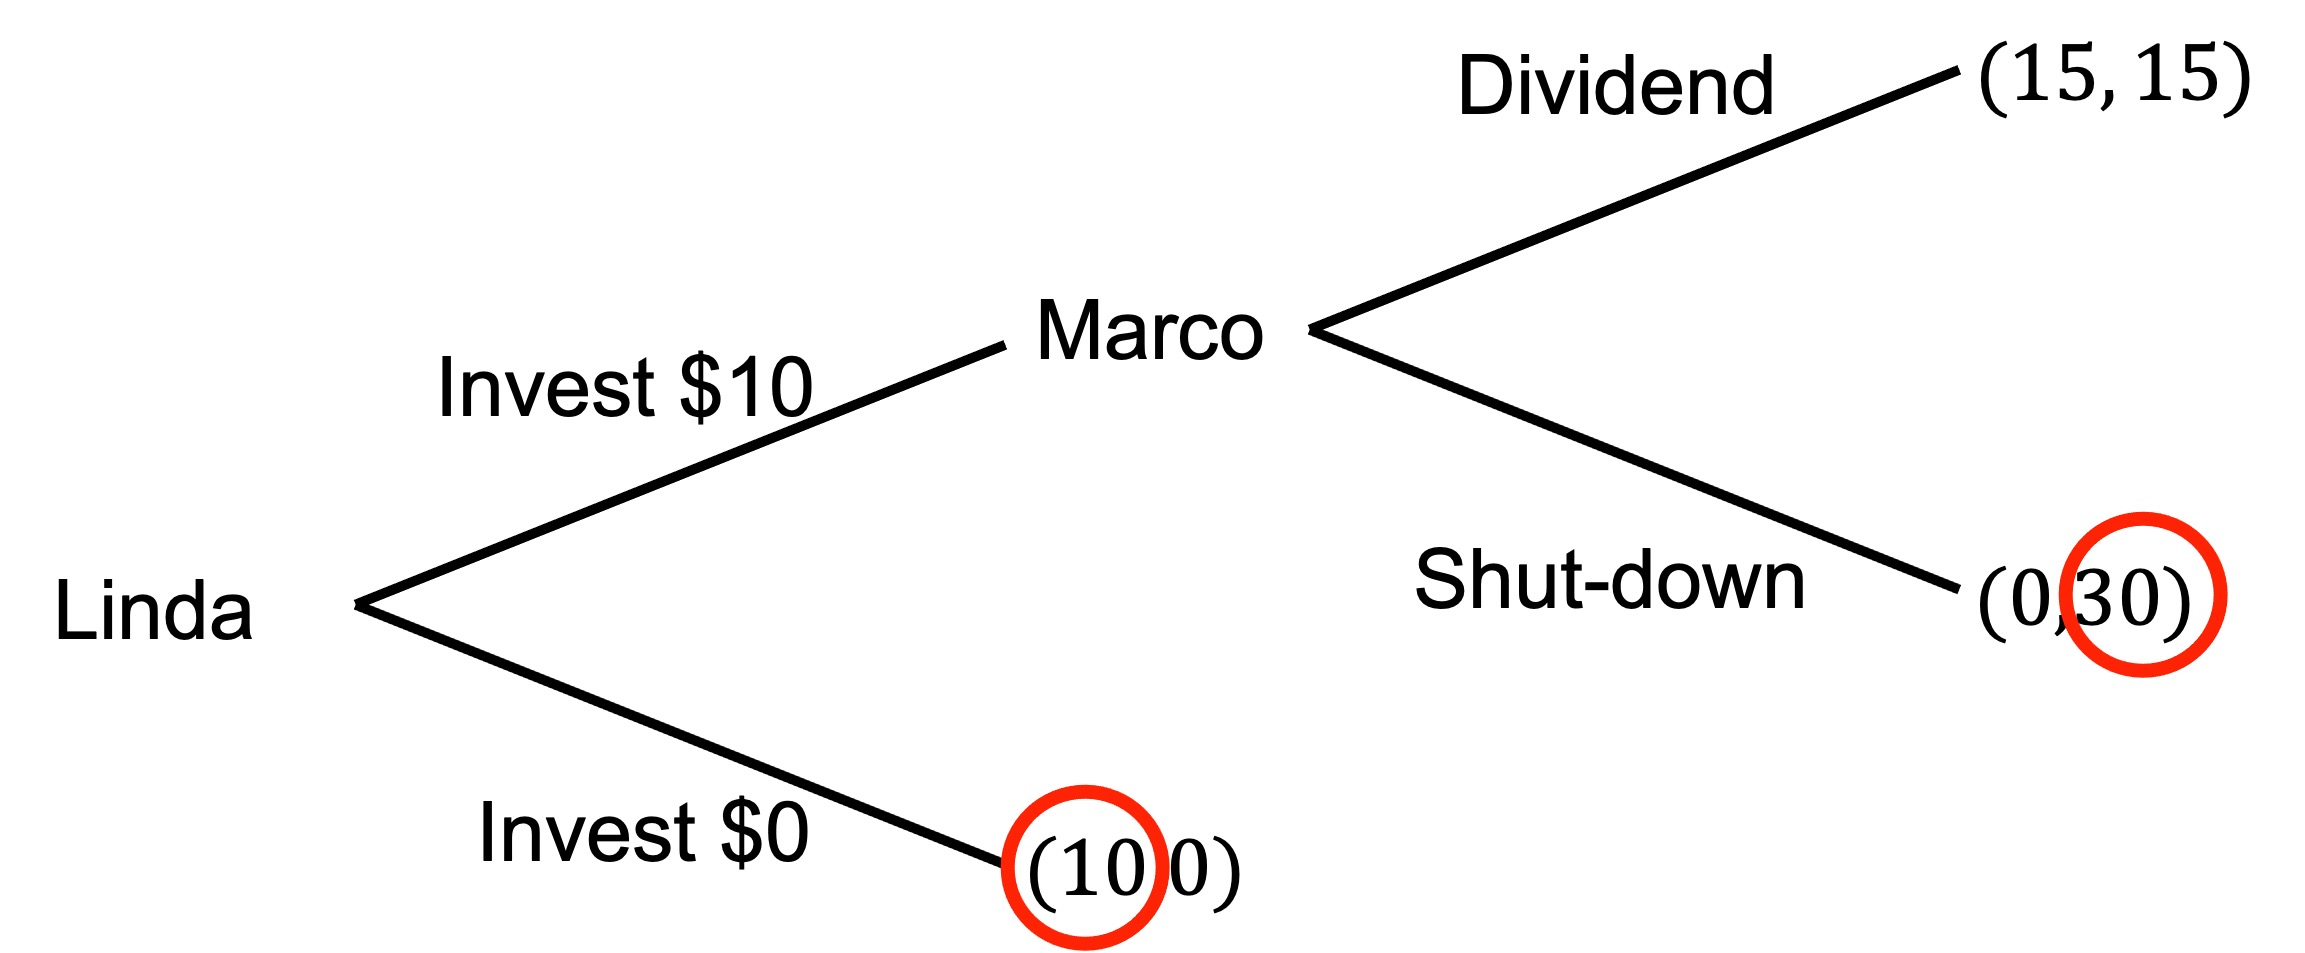
\includegraphics{game-theory/img/applied-trust-2.jpg}

\end{tcolorbox}

\hypertarget{war}{%
\section{War}\label{war}}

Two city states, Atlantis and El Dorado, are divided by a body of water.
In the middle is an island that both states claim sovereignty over.

To establish their claims, both states have built a bridge to the
island. Atlantis then sent troops to the island.

El Dorado is deciding whether to attack Atlantis's troops to reclaim the
island or to concede.

If El Dorado attacks, Atlantis need to decide whether to defend against
the attack or to retreat back across the bridge.

If El Dorado attacks and Atlantis defends, both countries will suffer
large losses.

These decisions and the payoffs (\(x,y\)) from each decision for El
Dorado and Atlantis respectively are as follows.

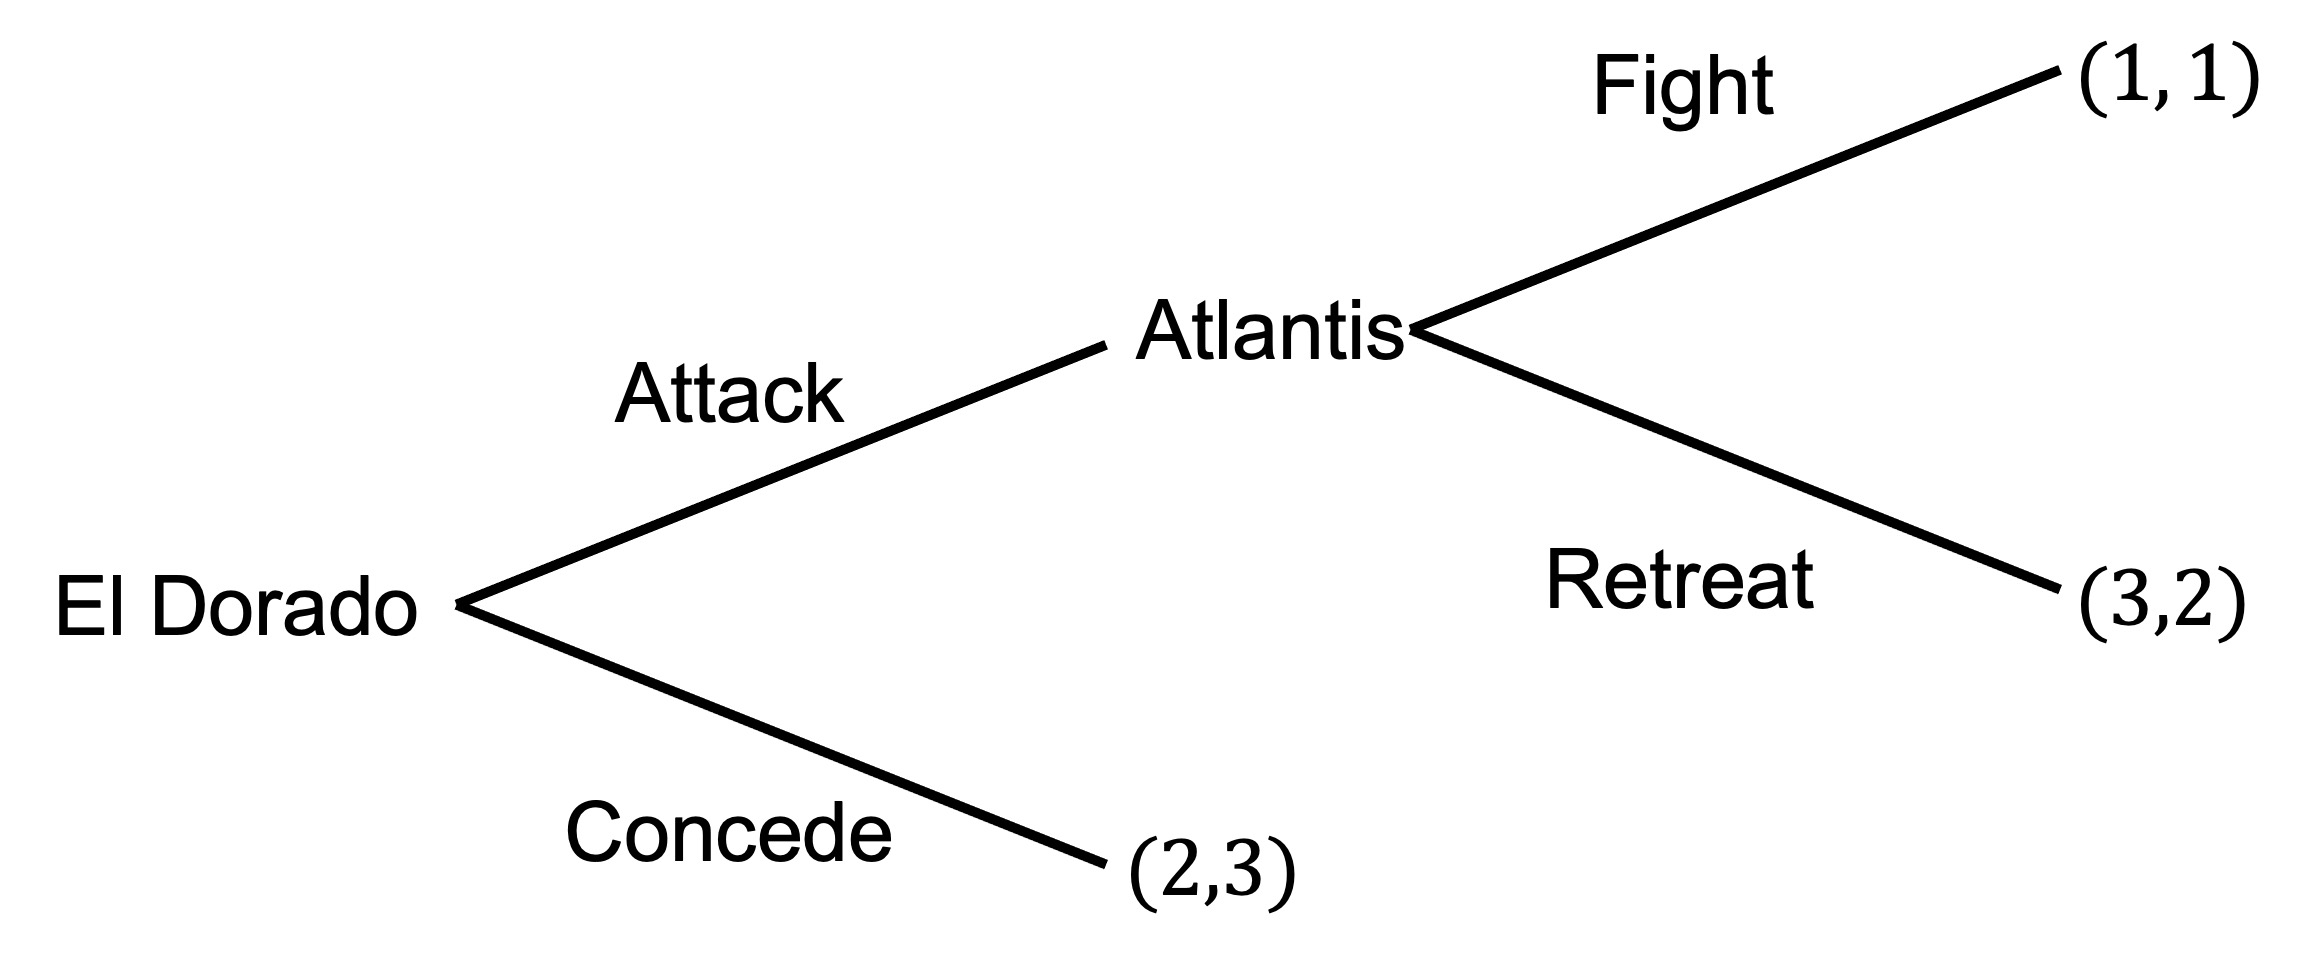
\includegraphics{game-theory/img/island-1.jpg}

a) What is the subgame-perfect equilibrium of this game?

\begin{tcolorbox}[enhanced jigsaw, title=\textcolor{quarto-callout-tip-color}{\faLightbulb}\hspace{0.5em}{Answer}, toprule=.15mm, colback=white, breakable, titlerule=0mm, colframe=quarto-callout-tip-color-frame, coltitle=black, opacityback=0, rightrule=.15mm, colbacktitle=quarto-callout-tip-color!10!white, bottomtitle=1mm, opacitybacktitle=0.6, arc=.35mm, bottomrule=.15mm, toptitle=1mm, leftrule=.75mm, left=2mm]

By backward induction, Atlantis would prefer to retreat (payoff of 2)
compared to fighting (payoff of 1). El Dorado then has a choice between
attacking (payoff of 3) and conceding (payoff of 2). El Dorado attacks.

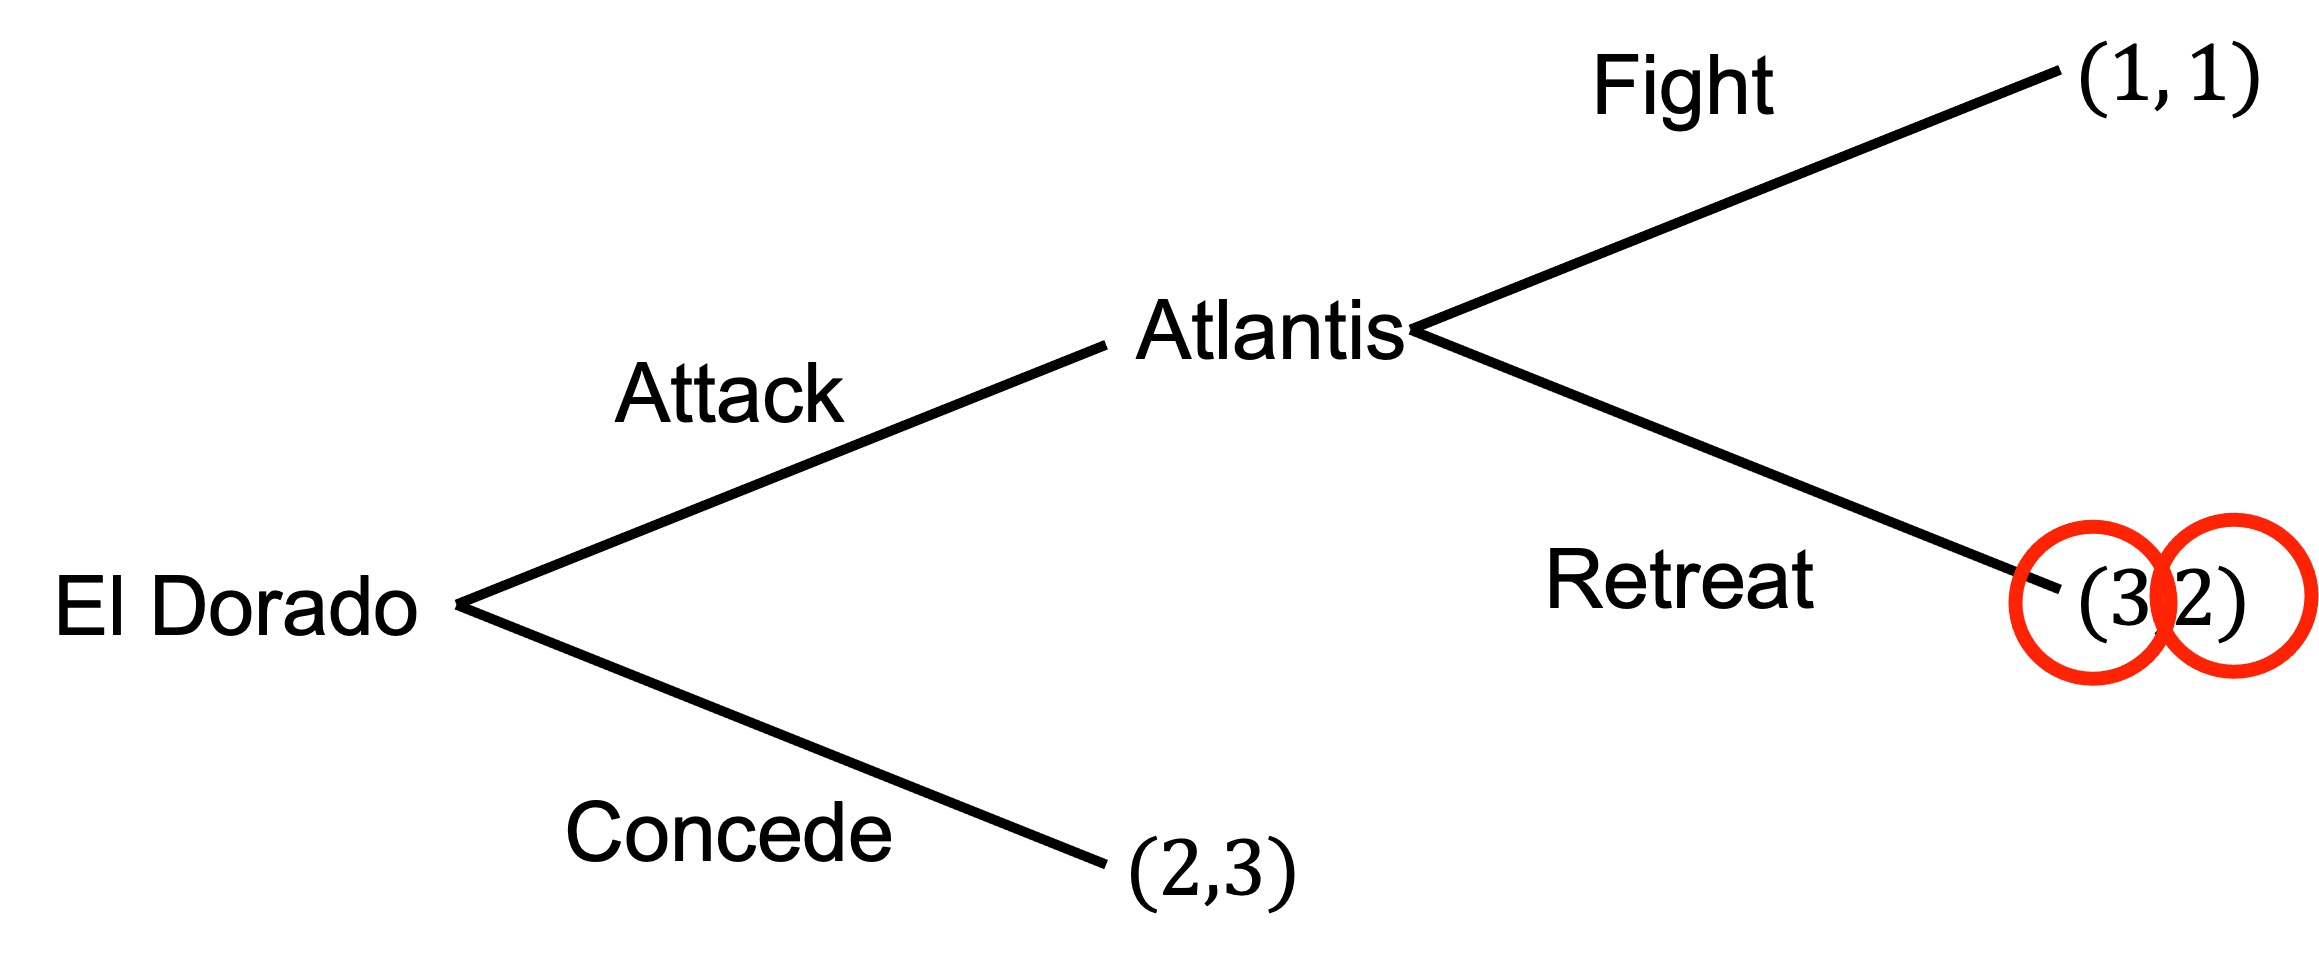
\includegraphics{game-theory/img/island-2.jpg}

The subgame-perfect equilbrium is (Attack, Retreat).

\end{tcolorbox}

b) An adviser to the Atlantis army suggests that they burn the bridge
behind them to remove the option of retreat.

Draw the new extensive form game that would emerge if Atlantis had the
option of the burning the bridge. What is the subgame-perfect
equilibrium?

\begin{tcolorbox}[enhanced jigsaw, title=\textcolor{quarto-callout-tip-color}{\faLightbulb}\hspace{0.5em}{Answer}, toprule=.15mm, colback=white, breakable, titlerule=0mm, colframe=quarto-callout-tip-color-frame, coltitle=black, opacityback=0, rightrule=.15mm, colbacktitle=quarto-callout-tip-color!10!white, bottomtitle=1mm, opacitybacktitle=0.6, arc=.35mm, bottomrule=.15mm, toptitle=1mm, leftrule=.75mm, left=2mm]

The new game is as follows (maintaining the payoffs as \(x,y\) for El
Dorado and Atlantis respectively):

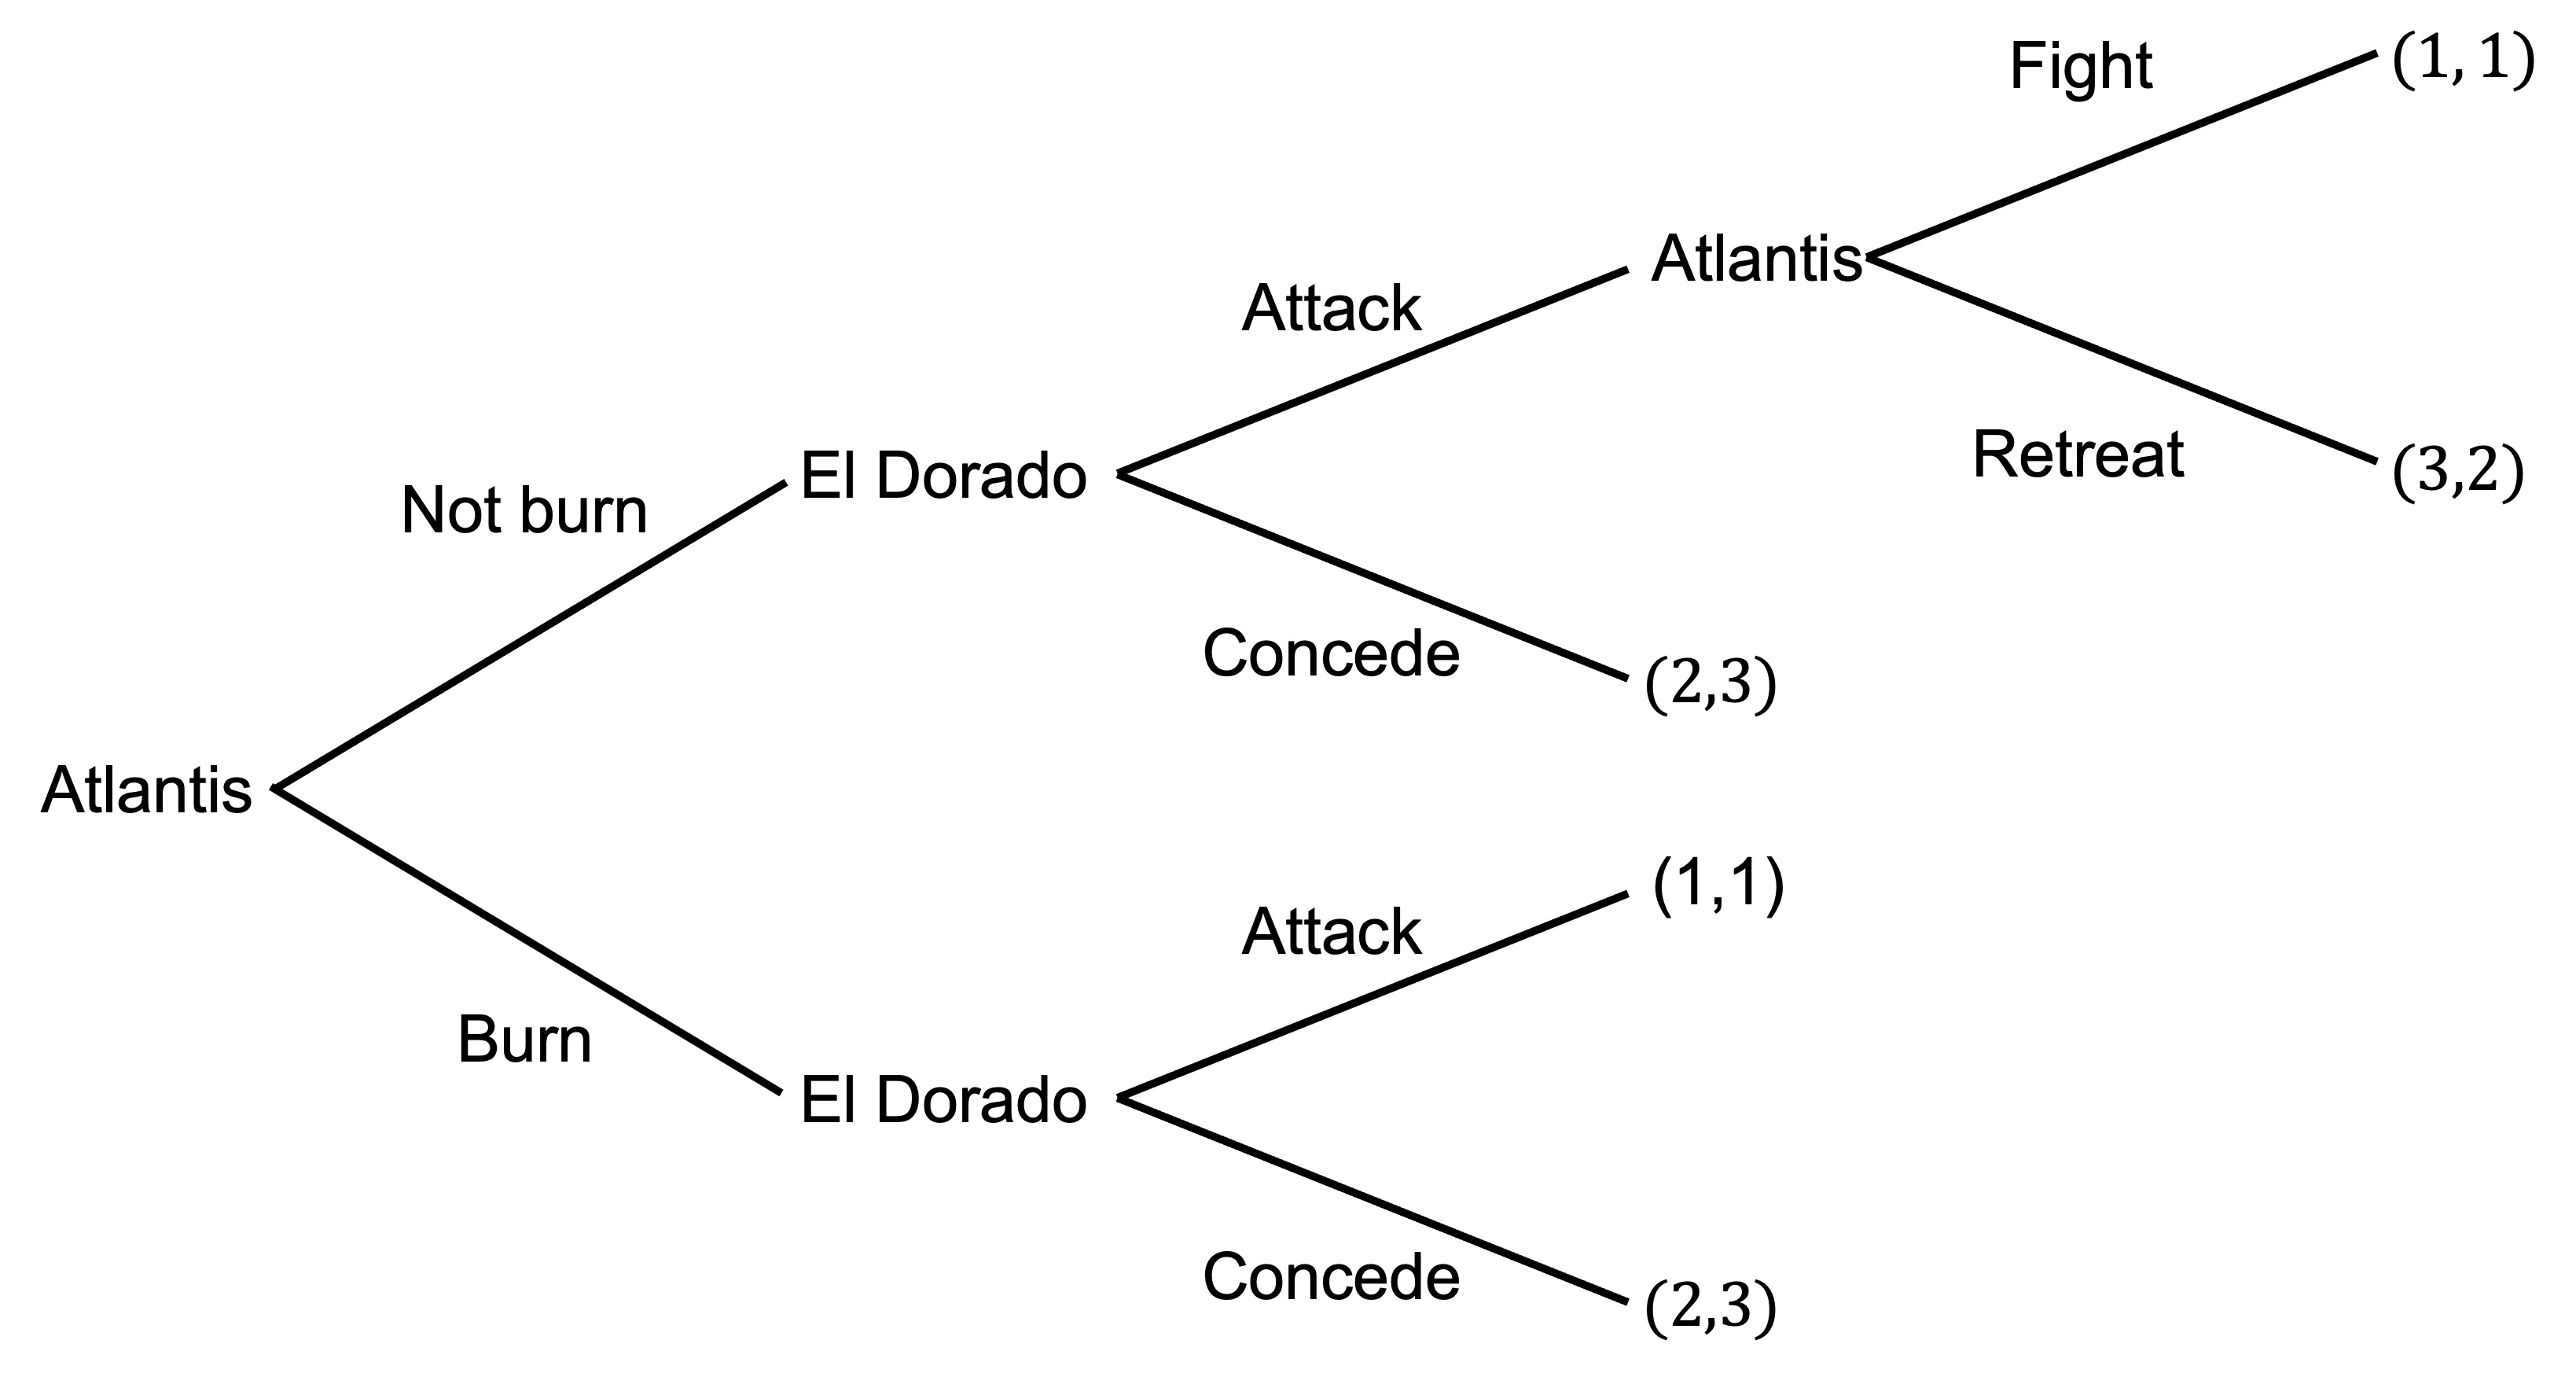
\includegraphics{game-theory/img/island-3.jpg}

If we work through this game by backward induction, starting with the
upper branch:

\begin{itemize}
\item
  Atlantis would prefer to retreat (payoff of 2) compared to fighting
  (payoff of 1).
\item
  El Dorado would prefer to attack (payoff of 3) compared to conceding
  (payoff of 2).
\end{itemize}

For the lower branch:

\begin{itemize}
\tightlist
\item
  El Dorado would prefer to concede (payoff of 2) compated to attack
  (payoff of 1).
\end{itemize}

For Atlantis's final decision, they would prefer to burn (payoff of 3)
compared to not burning (payoff of 2).

Atlantis burns the bridge.

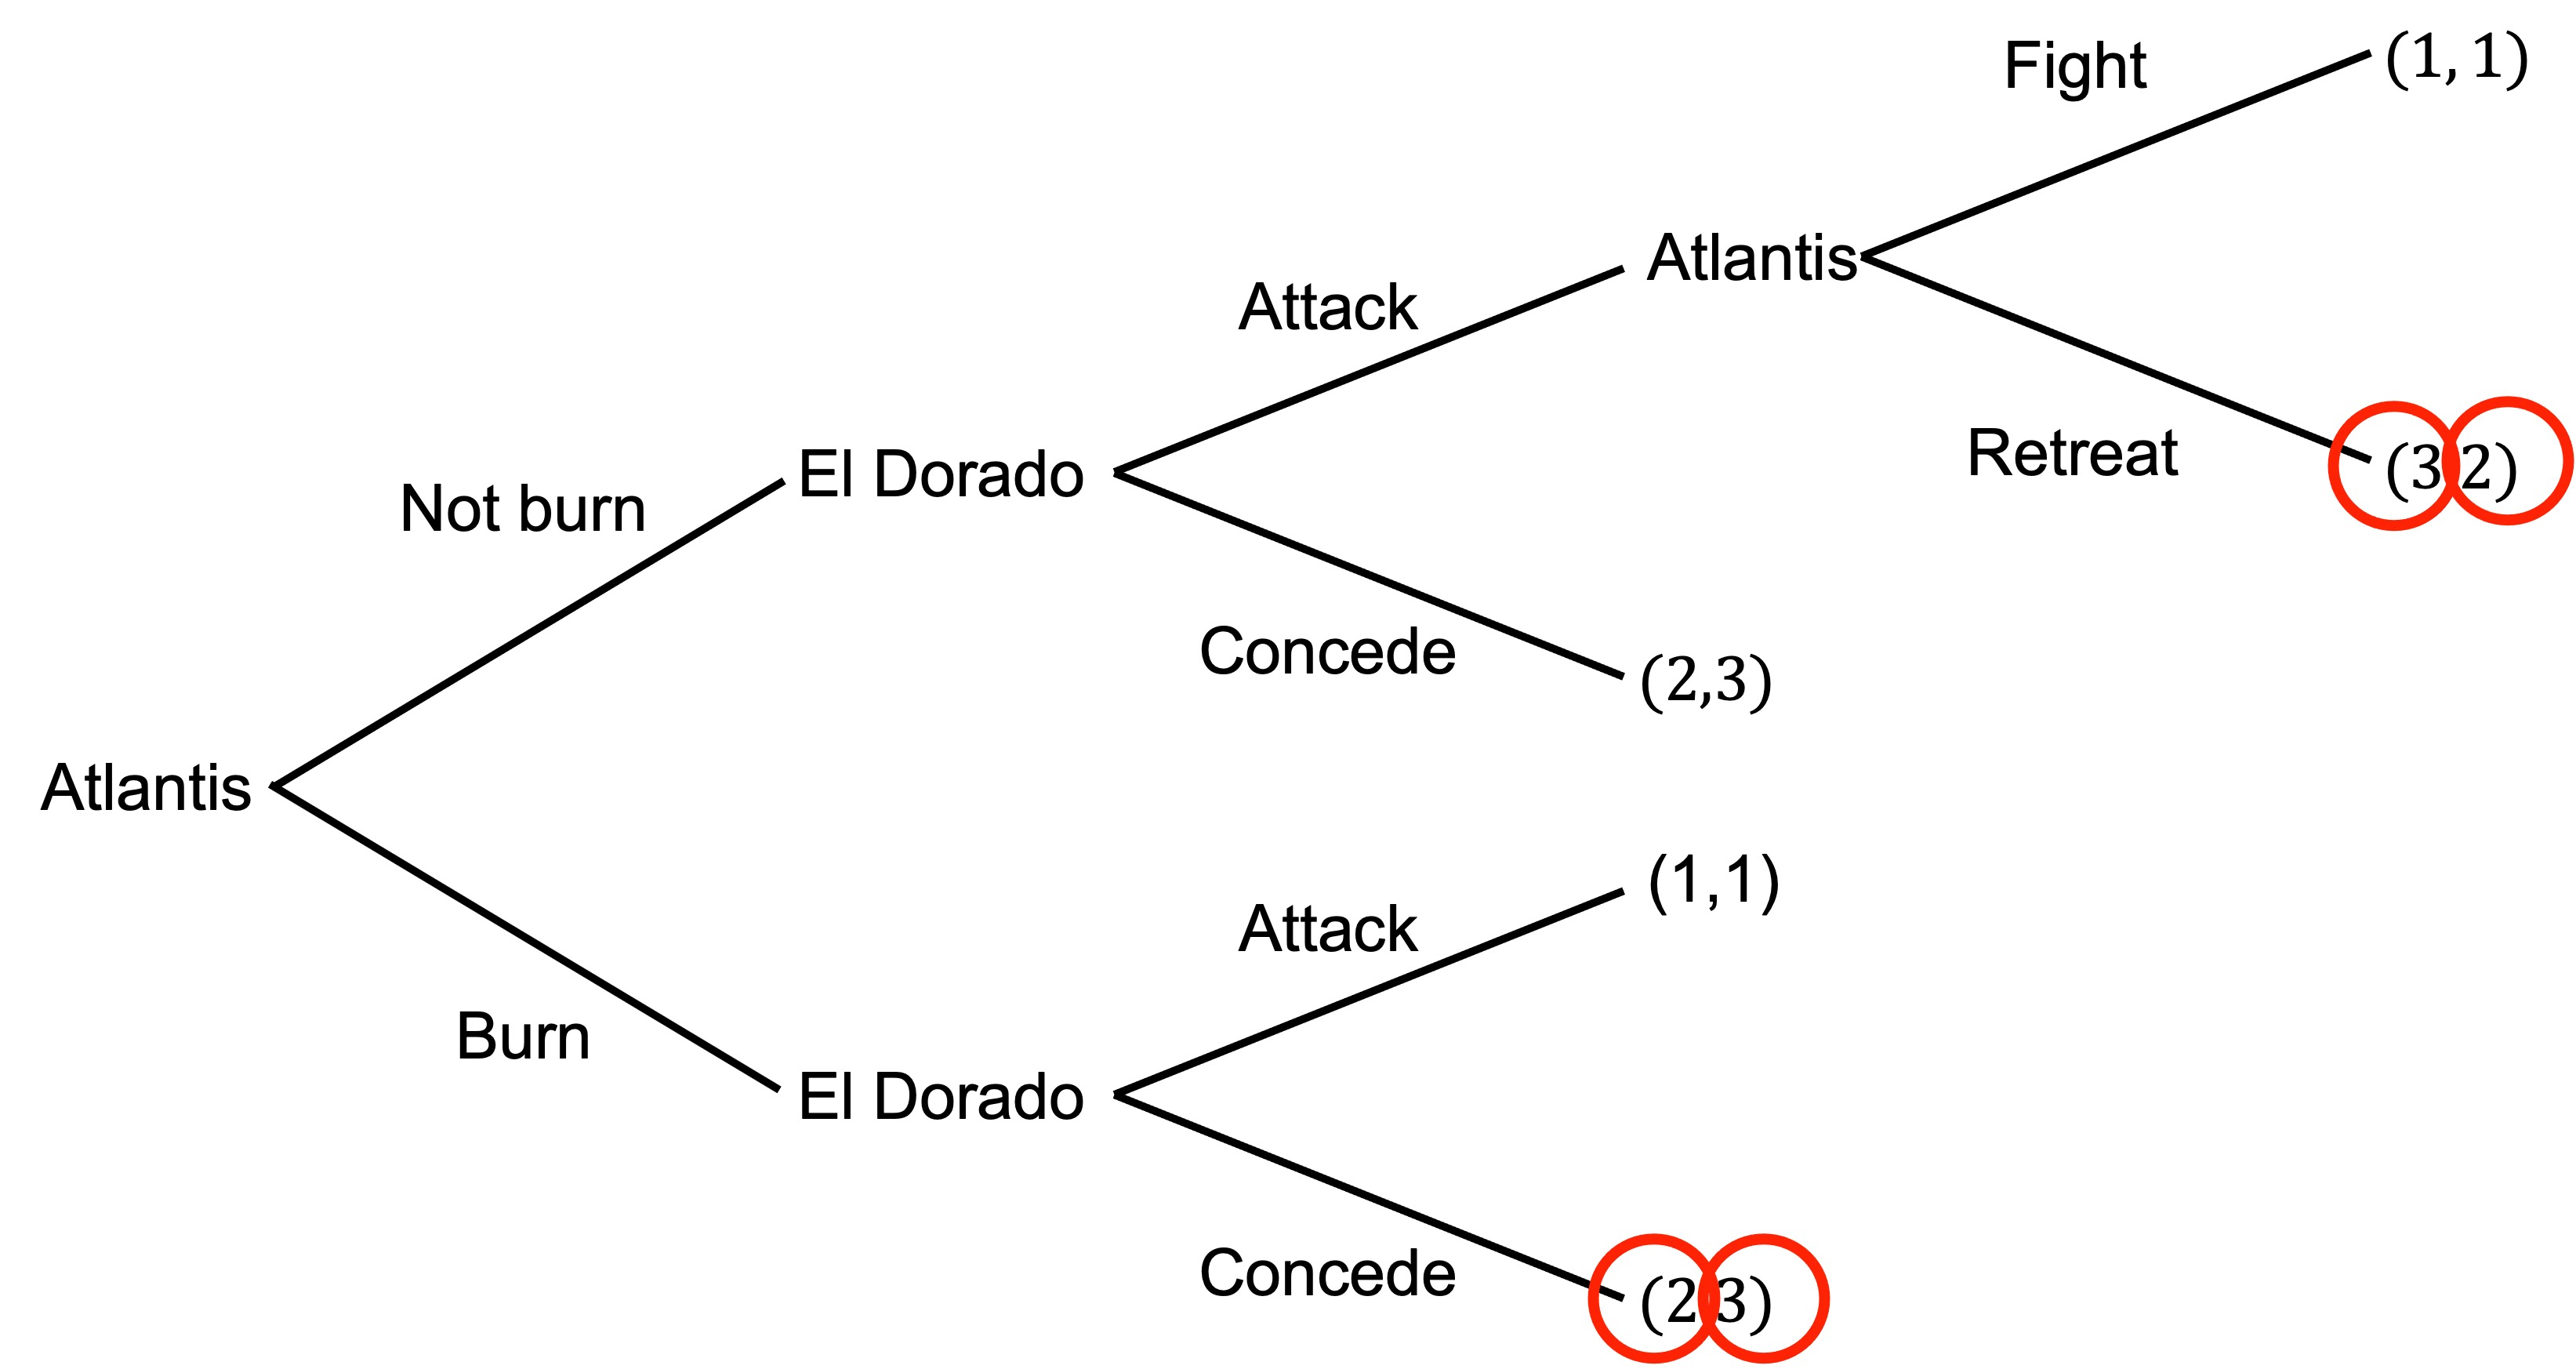
\includegraphics{game-theory/img/island-4.jpg}

The subgame-perfect equilibrium is (Burn, Retreat; Attack, Concede).

\end{tcolorbox}

\hypertarget{buying-a-car}{%
\section{Buying a car}\label{buying-a-car}}

Hayley wants to buy a car. The used-car salesman can sell her a good car
(for which he earns a small profit) or a lemon (for which he earns a
large profit).

The payoffs (x,y) for each decision are indicated in the game tree
below, with \(x\) being the Hayley's satisfaction and \(y\) being the
salesman's profit.

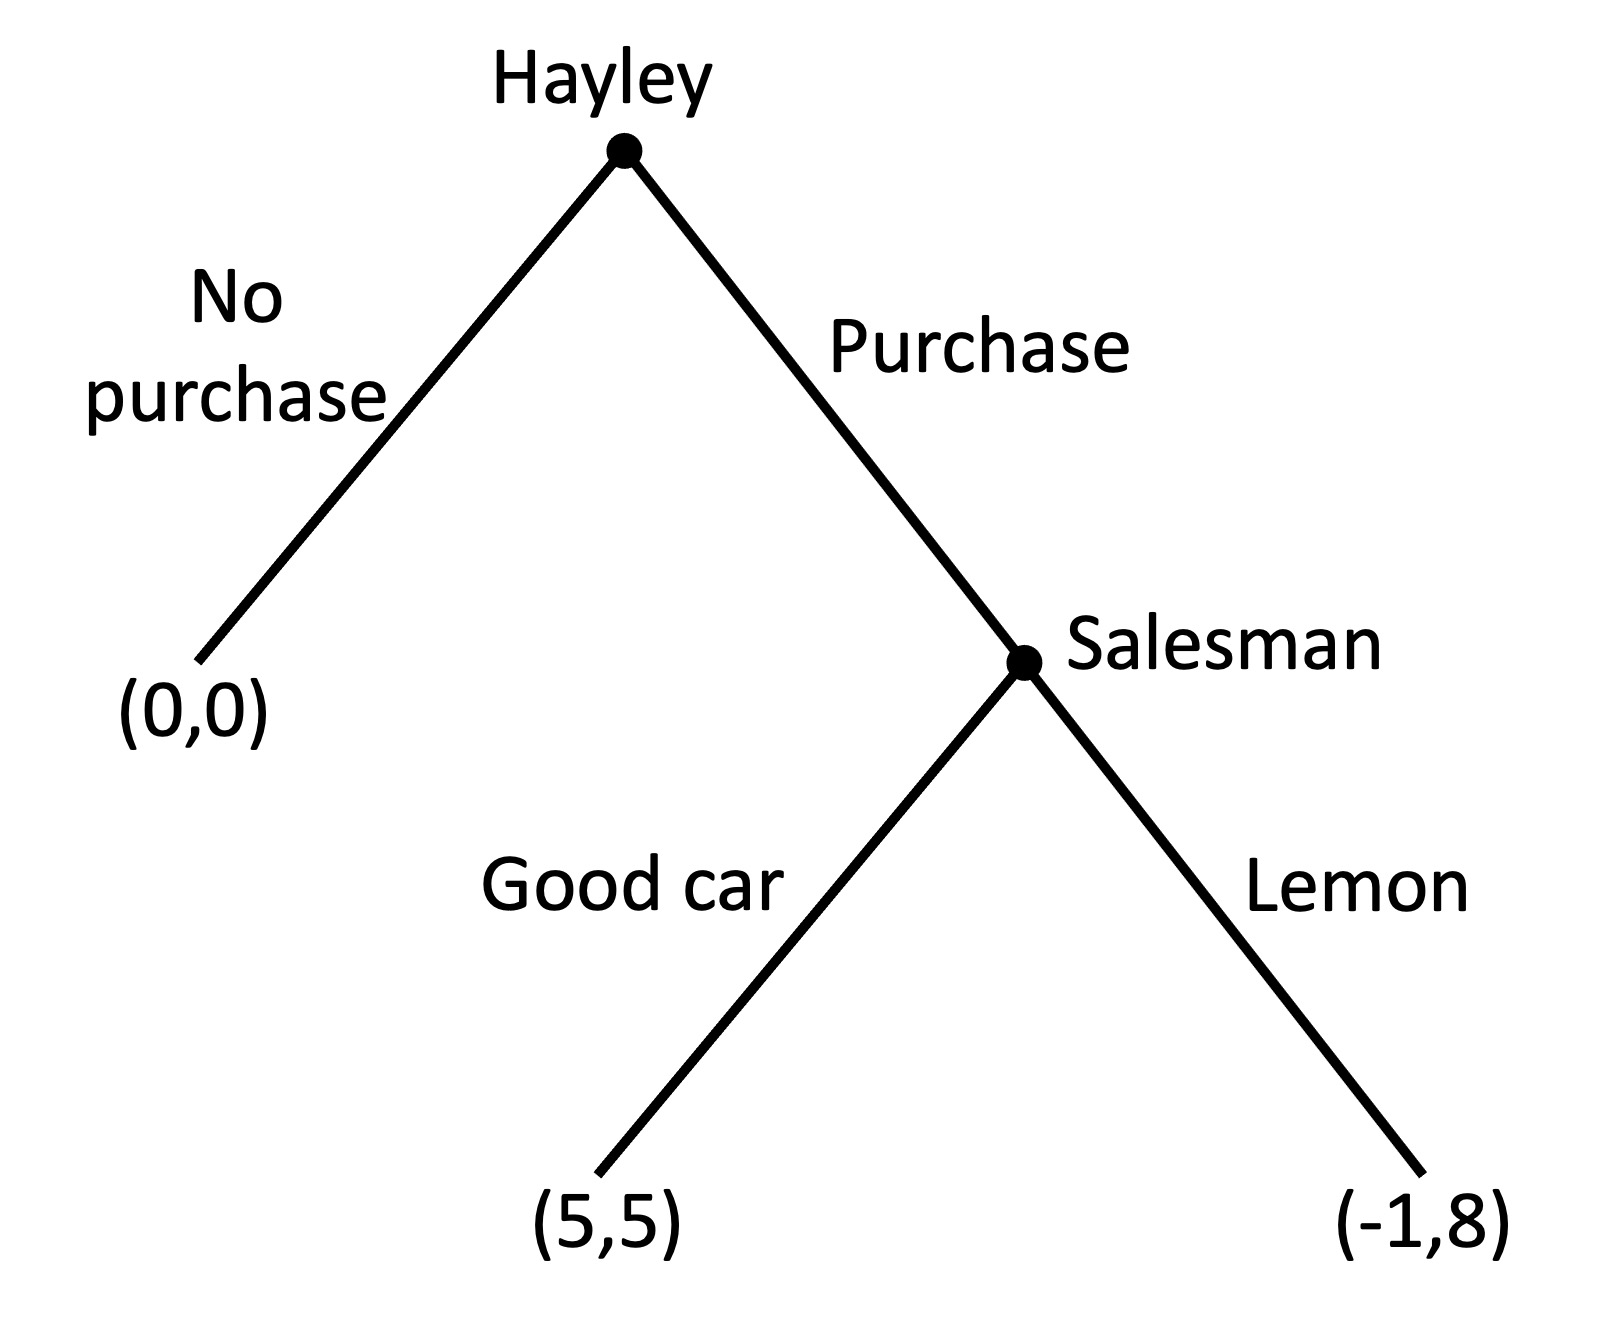
\includegraphics[width=0.6\textwidth,height=\textheight]{game-theory/img/car-1.jpg}

a) Assume the salesman only cares about his profit. What would the
salesman do if Hayley chooses to purchase? Why?

\begin{tcolorbox}[enhanced jigsaw, title=\textcolor{quarto-callout-tip-color}{\faLightbulb}\hspace{0.5em}{Answer}, toprule=.15mm, colback=white, breakable, titlerule=0mm, colframe=quarto-callout-tip-color-frame, coltitle=black, opacityback=0, rightrule=.15mm, colbacktitle=quarto-callout-tip-color!10!white, bottomtitle=1mm, opacitybacktitle=0.6, arc=.35mm, bottomrule=.15mm, toptitle=1mm, leftrule=.75mm, left=2mm]

The salesman will compare payoffs of 8 for selling a lemon and 5 for
selling a good car. He will choose to sell a lemon.

\end{tcolorbox}

b) Given the anticipated choice of the salesman, would Hayley purchase
the car? Why?

\begin{tcolorbox}[enhanced jigsaw, title=\textcolor{quarto-callout-tip-color}{\faLightbulb}\hspace{0.5em}{Answer}, toprule=.15mm, colback=white, breakable, titlerule=0mm, colframe=quarto-callout-tip-color-frame, coltitle=black, opacityback=0, rightrule=.15mm, colbacktitle=quarto-callout-tip-color!10!white, bottomtitle=1mm, opacitybacktitle=0.6, arc=.35mm, bottomrule=.15mm, toptitle=1mm, leftrule=.75mm, left=2mm]

Hayley will compare a payoff of 0 for no purchase and a payoff of -1 for
buying a car that will be a lemon. She chooses not to purchase.

\end{tcolorbox}

c) Suppose Hayley can take legal action if she is sold a lemon. If
Hayley is successful in court, she will be refunded the purchase price
but would suffer a cost of -5 due to the effort involved. Would this
change the outcome? Why?

\begin{tcolorbox}[enhanced jigsaw, title=\textcolor{quarto-callout-tip-color}{\faLightbulb}\hspace{0.5em}{Answer}, toprule=.15mm, colback=white, breakable, titlerule=0mm, colframe=quarto-callout-tip-color-frame, coltitle=black, opacityback=0, rightrule=.15mm, colbacktitle=quarto-callout-tip-color!10!white, bottomtitle=1mm, opacitybacktitle=0.6, arc=.35mm, bottomrule=.15mm, toptitle=1mm, leftrule=.75mm, left=2mm]

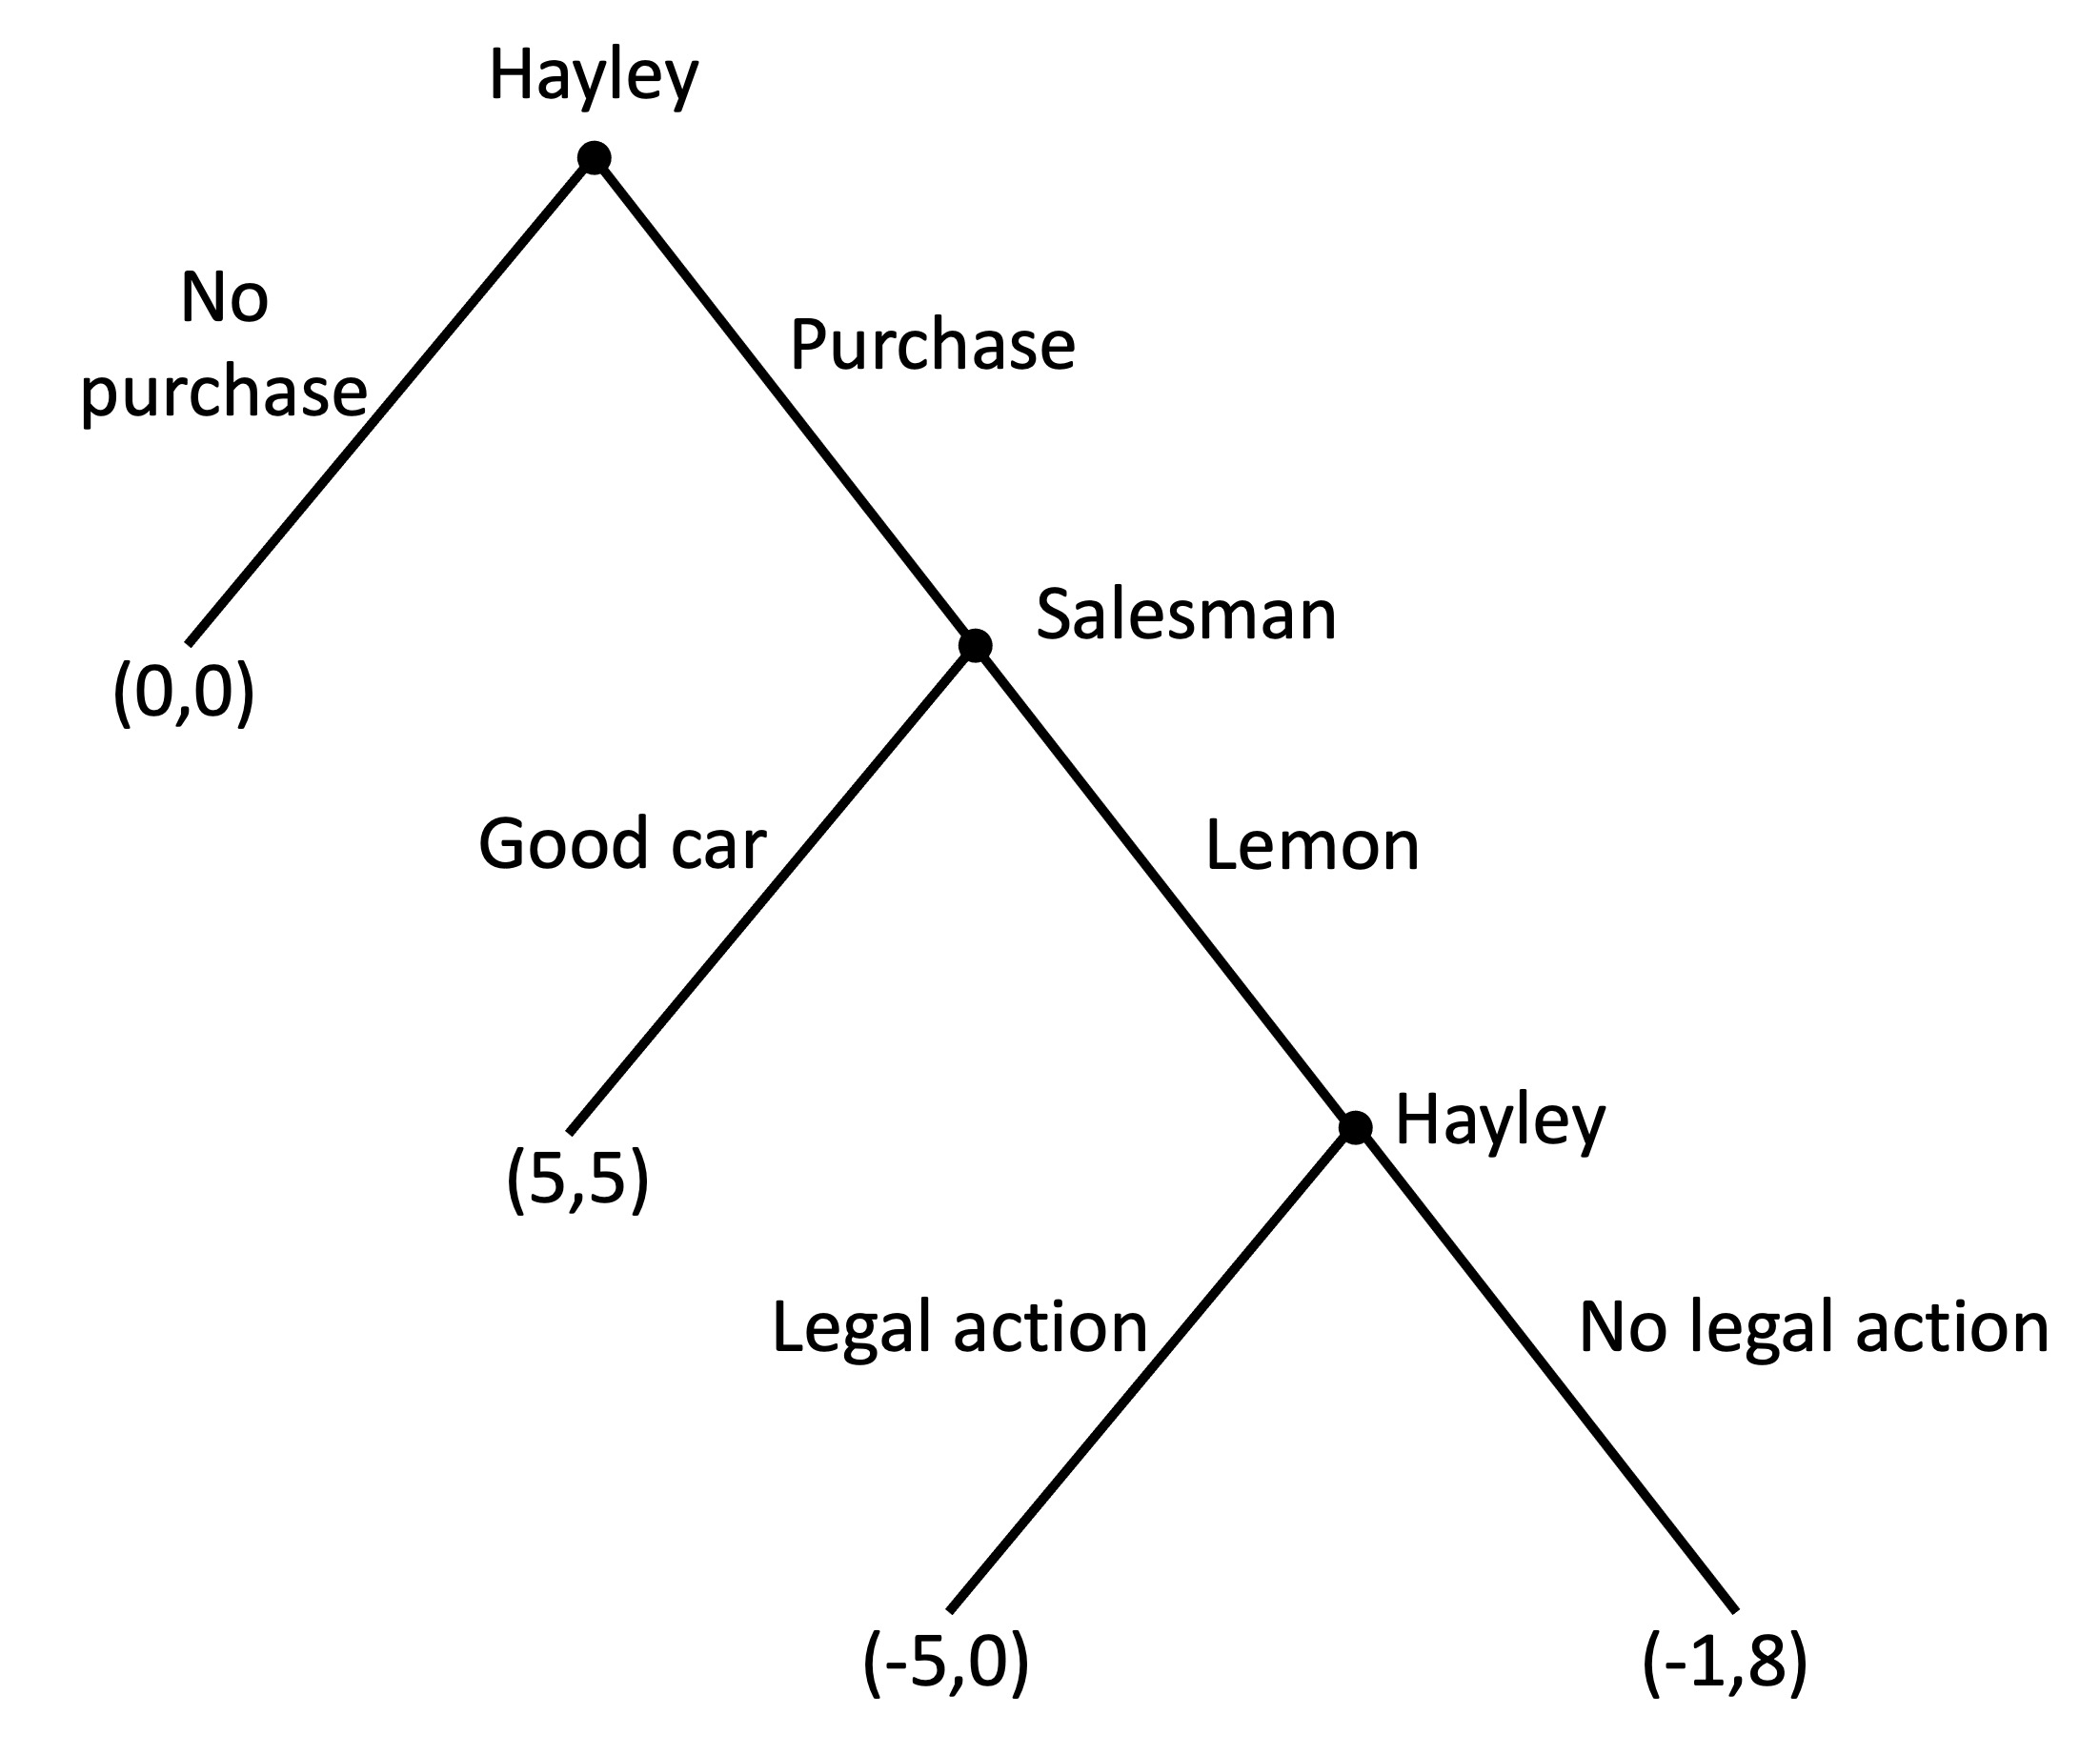
\includegraphics[width=0.8\textwidth,height=\textheight]{game-theory/img/car-2.jpg}

Working by backward induction, Hayley has a choice between taking legal
action for a payoff of -5 or not complaining for a payoff of -1. She
will not complain.

The rest of the game plays out as per questions a) and b). There is no
change to the outcome as she cannot commit to complain in advance. The
threat to take legal action is not credible.

\end{tcolorbox}

d) Suppose Hayley has a reputation of being quick to anger and always
carrying out her threats. Suppose Hayley would experience satisfaction
of +6 from taking legal action (in addition to the effort cost of -5).
The salesman knows this and believes it to be a credible commitment.
Would this change the outcome? Why?

\begin{tcolorbox}[enhanced jigsaw, title=\textcolor{quarto-callout-tip-color}{\faLightbulb}\hspace{0.5em}{Answer}, toprule=.15mm, colback=white, breakable, titlerule=0mm, colframe=quarto-callout-tip-color-frame, coltitle=black, opacityback=0, rightrule=.15mm, colbacktitle=quarto-callout-tip-color!10!white, bottomtitle=1mm, opacitybacktitle=0.6, arc=.35mm, bottomrule=.15mm, toptitle=1mm, leftrule=.75mm, left=2mm]

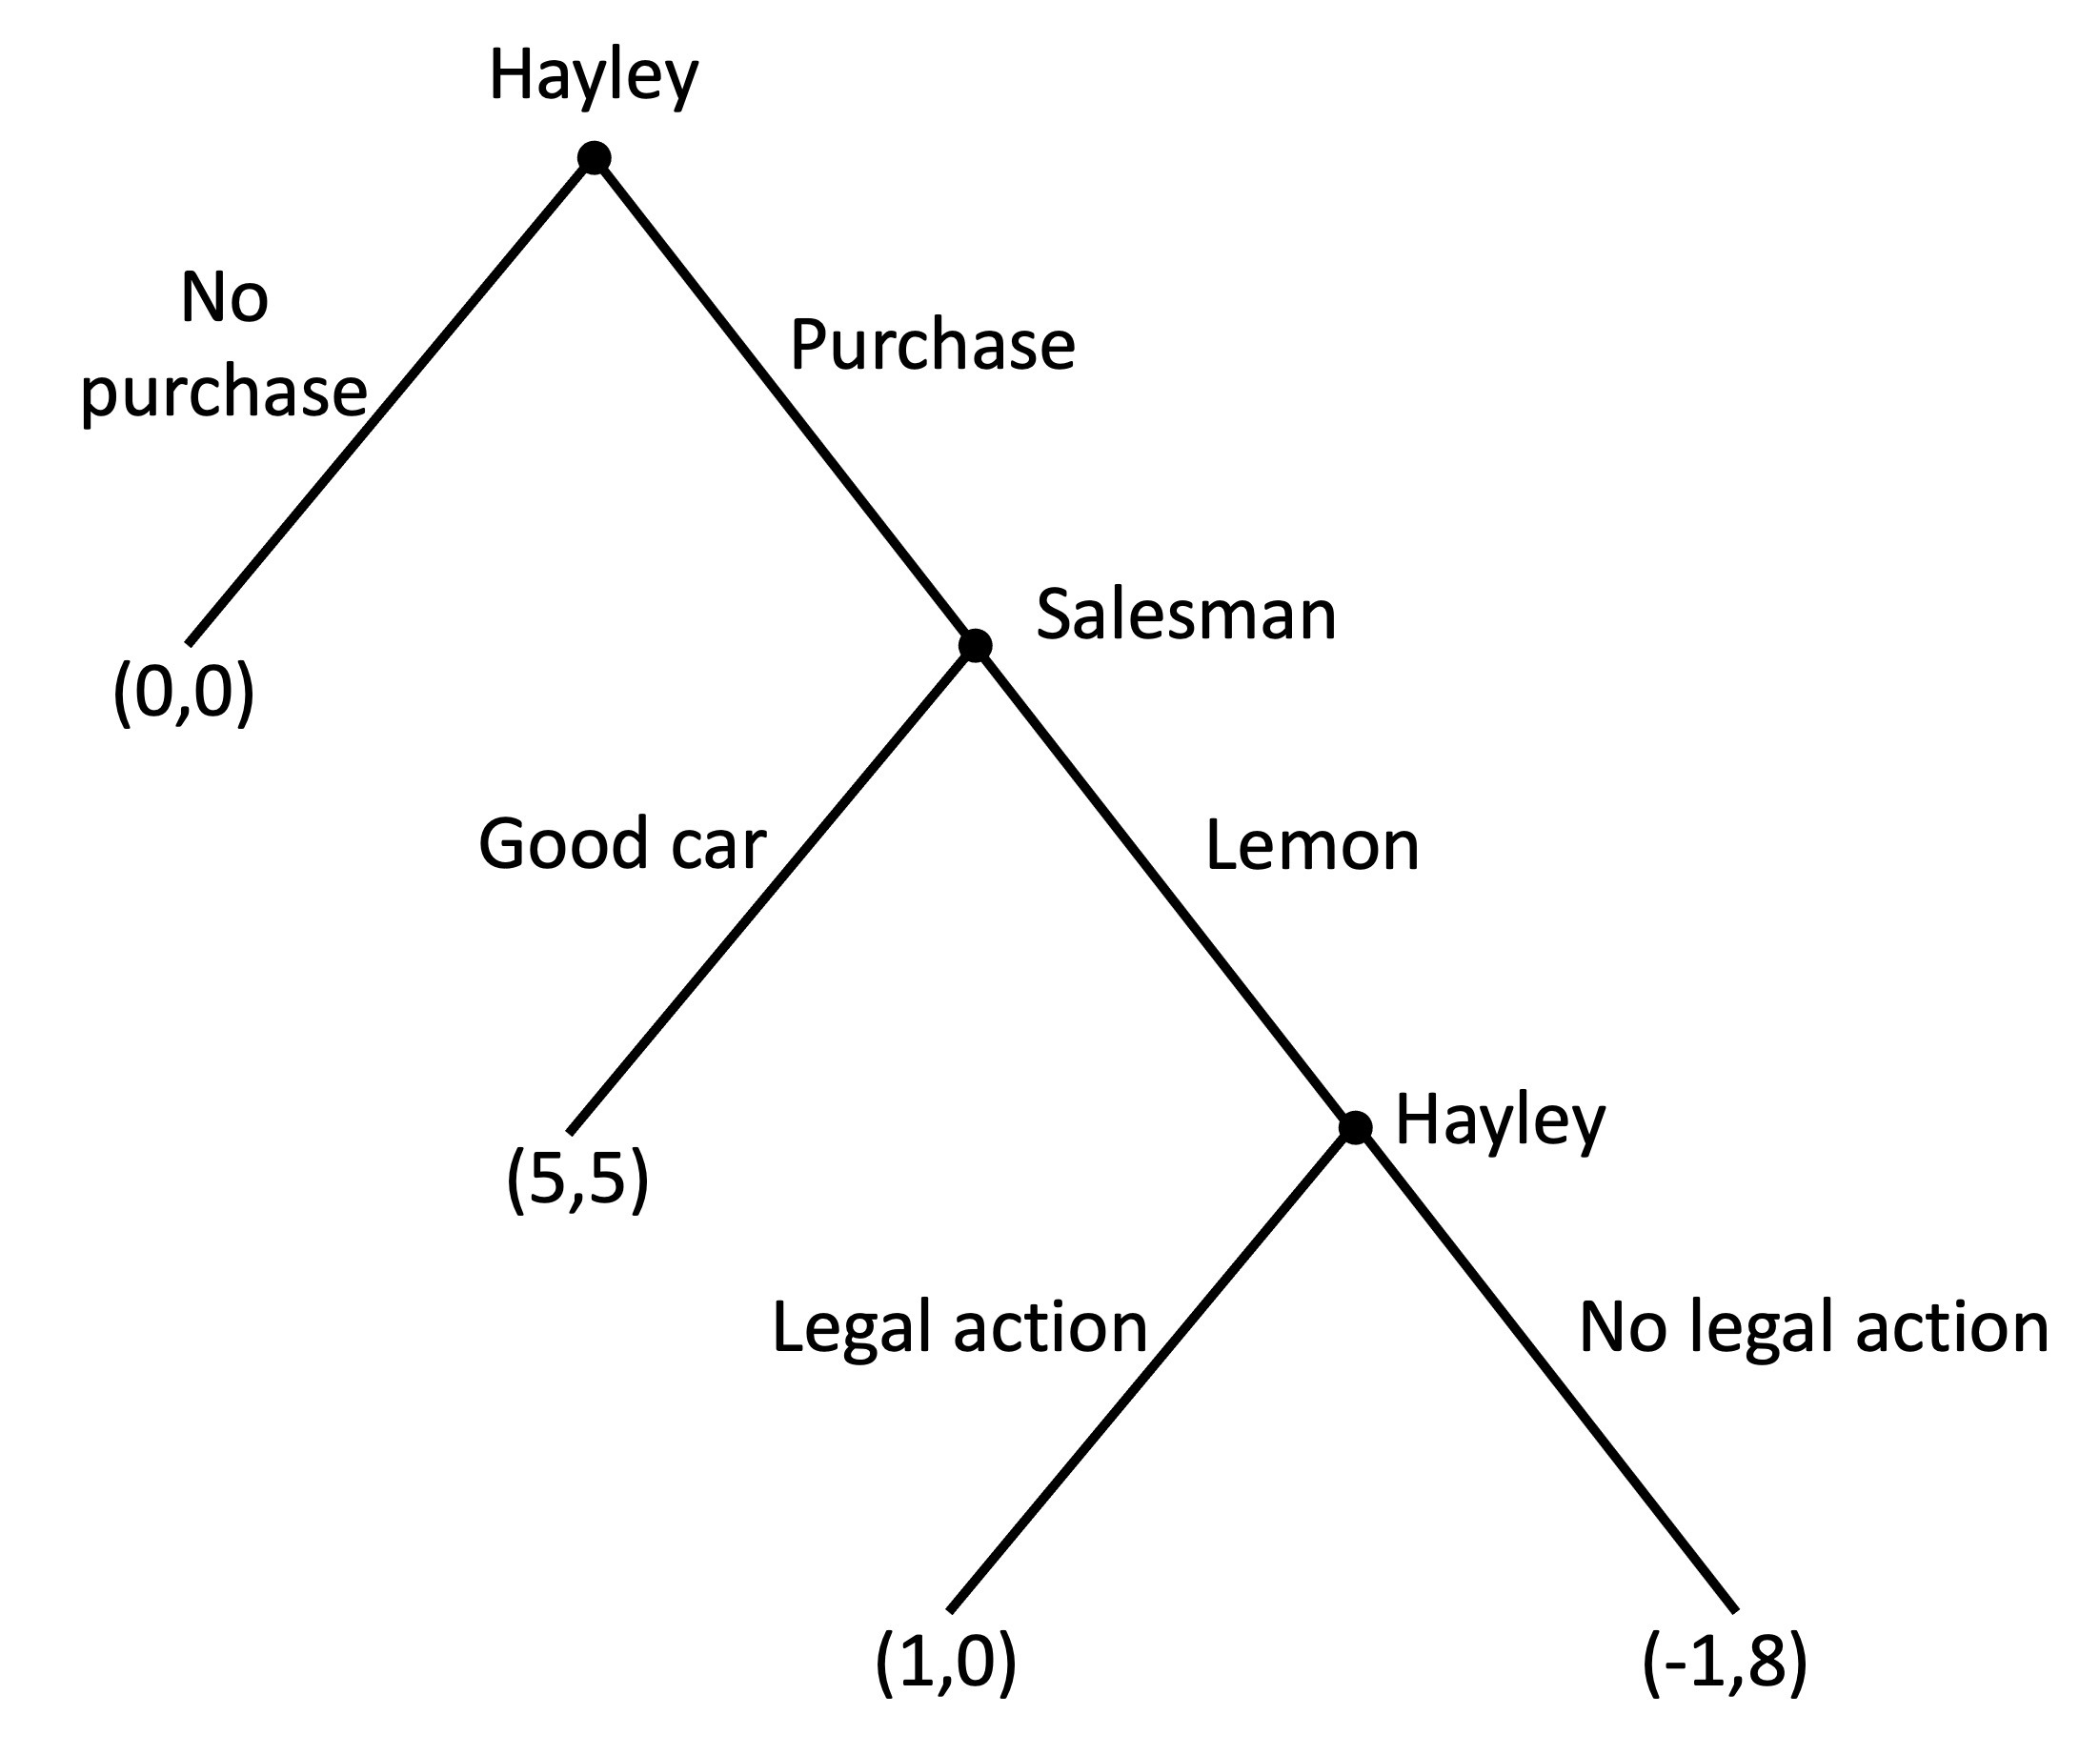
\includegraphics[width=0.8\textwidth,height=\textheight]{game-theory/img/car-3.jpg}

Hayley now has a choice between a payoff of 1 by taking legal action and
a payoff of -1 for accepting the lemon. She would take legal action.

The salesman now has a choice between a payoff of 0 for selling the
lemon (as Hayley takes legal action and the sale is refunded) and 5 for
selling a good car. He sells the good car

Hayley now has a choice of a payoff of 0 for not purchasing a car, and 5
for purchasing. She makes the purchase and gets a good car.

\end{tcolorbox}

\part{Behavioural game theory}

In our analysis of game theory, we have assumed rational agents in that
they use all available information and are able to successfully
determine their best action given their opponents (also rational)
action.

What if agents have limited rationality or vary in their rationality?

\hypertarget{level-k-thinking}{%
\chapter{Level-k thinking}\label{level-k-thinking}}

The idea behind level-k thinking is that a player forms an expectation
of what others will do and tries to be ``one step ahead''.

A level-k player best-responds to level-(k-1) players.

Level-0 players do not engage in strategic thinking. This is usually
modelled as randomisation across all strategies. For example, in the
beauty contest this implies the selection of a number between 0 and 100
with equal probability.

Level-1 players assume other players are level-0 and act optimally
conditional on this assumption.

Level-2 players assume other players are level-1 and act optimally
conditional on this assumption.

\hypertarget{the-beauty-contest}{%
\section{The beauty contest}\label{the-beauty-contest}}

From Keynes (1936):

\begin{quote}
{[}P{]}rofessional investment may be likened to those newspaper
competitions in which the competitors have to pick out the six prettiest
faces from a hundred photographs, the prize being awarded to the
competitor whose choice most nearly corresponds to the average
preferences of the competitors as a whole; so that each competitor has
to pick, not those faces which he himself finds prettiest, but those
which he thinks likeliest to catch the fancy of the other competitors,
all of whom are looking at the problem from the same point of view. It
is not a case of choosing those which, to the best of one's judgment,
are really the prettiest, nor even those which average opinion genuinely
thinks the prettiest. We have reached the third degree where we devote
our intelligences to anticipating what average opinion expects the
average opinion to be. And there are some, I believe, who practise the
fourth, fifth and higher degrees.
\end{quote}

This thought experiment has since been developed into a game, the
p-beauty contest (Moulin (1986)). The p-beauty contest runs as follows:

Each of \(n\) players pick a number \(y\in[0,100]\).

The winner is the player whose chosen number is closest to the mean of
all the chosen numbers (\(\bar y\)) multiplied by a parameter \(p\).

That is, the winner is the player with their chosen number closest to
\(p\bar y\).

\(p\) is typically chosen such \(0\leq p\leq 1\), with \(p=1/2\) and
\(p=2/3\) common.

Each player should play \(y_i=0\). This is the Nash equilibrium for the
game. But what actually occurs?

The following charts come from Nagel (1995).

\begin{figure}

\begin{minipage}[t]{0.50\linewidth}

{\centering 

\raisebox{-\height}{

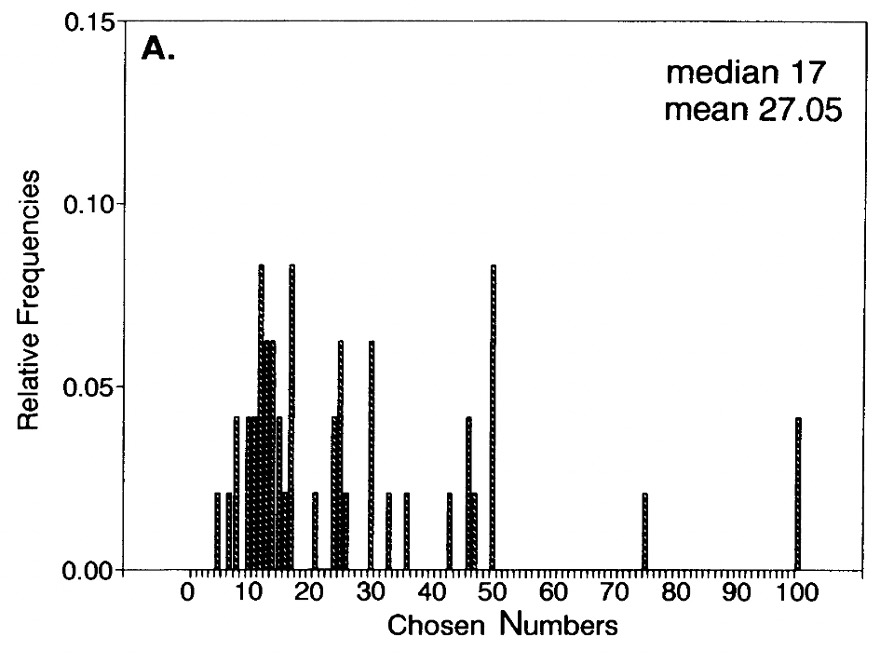
\includegraphics{behavioural-game-theory/img/nagel-1995-12.jpg}

}

\caption{\(p=1/2\)}

}

\end{minipage}%
%
\begin{minipage}[t]{0.50\linewidth}

{\centering 

\raisebox{-\height}{

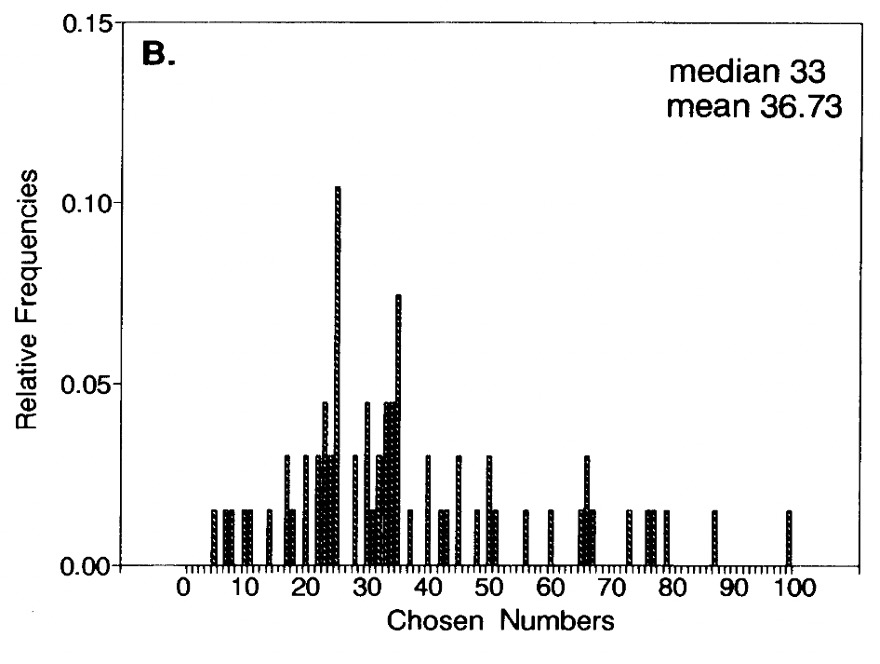
\includegraphics{behavioural-game-theory/img/nagel-1995-23.jpg}

}

\caption{\(p=2/3\)}

}

\end{minipage}%

\caption{\label{fig-nagel1}Choices by players of the p-beauty game}

\end{figure}

Suppose \(p=2/3\).

Level-0: Players randomly select a number in the interval {[}0, \ldots,
100{]}.

Level-1: If level-0 players select across the interval {[}0, \ldots,
100{]}, the best response is:

\[
y_1=\frac{2}{3}\bar y=\frac{2}{3}\times 50=33.3
\]

Level-2: Assume all other players are level-1 and select 33.3, so the
best response is:

\[
y_2=\frac{2}{3}\bar y=2/3\times 33.3=22.2
\]

Level-3: Assume all other players are level-2 and select 22.2, so the
best response is:

\[
y_3=\frac{2}{3}\bar y=2/3\times 22.2=14.8
\]

And so on.

Looking at experimental data with the filter of level-k theory, there
are few level-0 players. Most are level-1, level-2 and level-3 players.
For example, the data shown above reported in Nagel (1995) where
\(p=2/3\) shows a spike at 33.3, indicative of level-1 players and
another at 22.2, indicative of level-2 players.

The lab evidence doesn't necessarily imply level-k is ``right model''.
Data and theory appear to match but it is hard to know whether this is
how subjects are thinking.

\hypertarget{the-assignment-game-with-level-k-thinking}{%
\section{The assignment game with level-k
thinking}\label{the-assignment-game-with-level-k-thinking}}

Consider the following game:

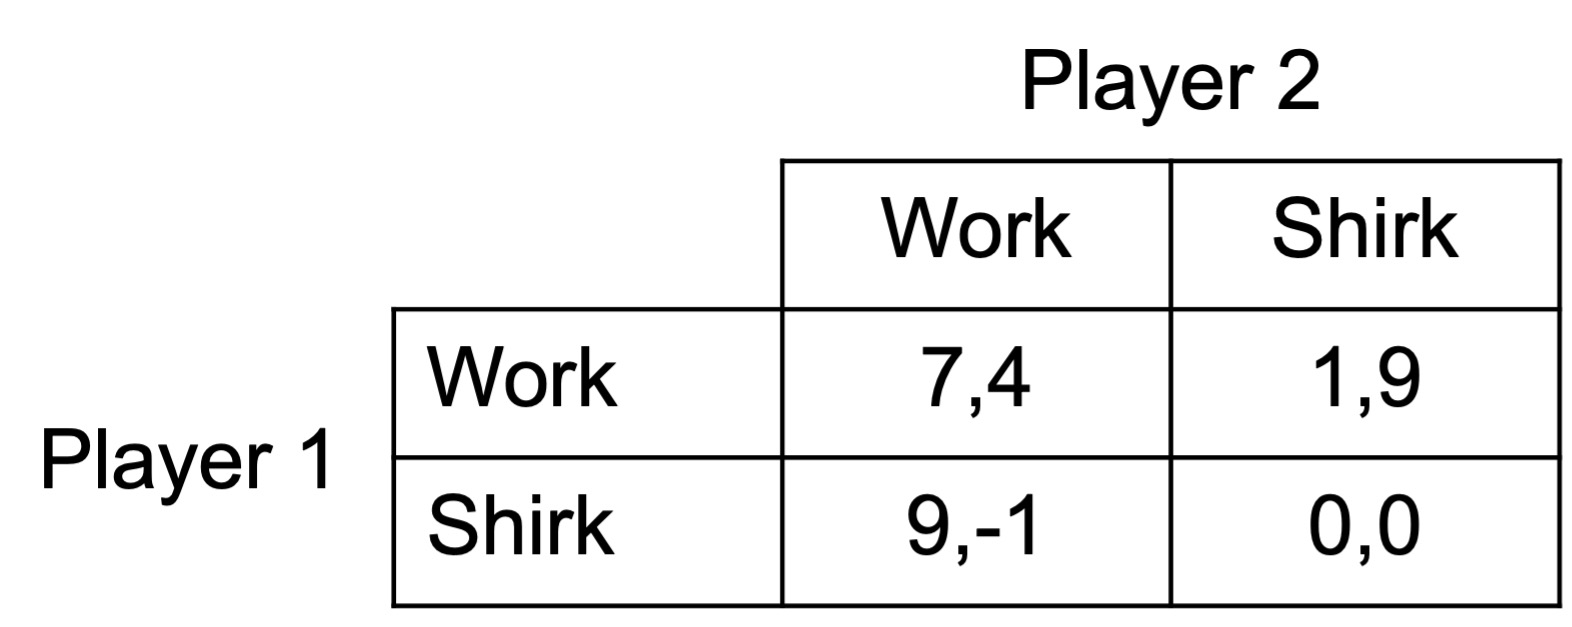
\includegraphics[width=0.6\textwidth,height=\textheight]{behavioural-game-theory/img/assignment-1.jpg}

There is a unique Nash equilibrium (work, shirk) with shirk dominant
strategy for Player 2

With a level-k model the outcome depends on the assumption on players'
level-k. When level-k thinking is introduced, the symmetries required by
Nash Equilbrium break apart.

If a player has a dominant strategy, they ``discover'' it at \(k=1\) and
always uses it for \(k\geq 1\).

Here, Nash equilibrium requires a \(k\geq 2\) level of thinking. Nash
equilibrium is the best people can do conditional on the strategy
selected by other players.

If players endowed with level \(k=\bar k\) rationality play Nash, all
players with \(k>\bar k\) play Nash.

\begin{longtable}[]{@{}lll@{}}
\toprule()
Level-k & Player 1 & Player 2 \\
\midrule()
\endhead
\(k=0\) & Random & Random \\
\(k=1\) & Shirk & Shirk \\
\(k=2\) & Work & Shirk \\
\bottomrule()
\end{longtable}

\hypertarget{centipede-game}{%
\section{Centipede game}\label{centipede-game}}

Recall the centipede game.

This centipede game has six stages. At each stage, a player can ``take''
and end the game or they can ``pass'', increasing the total payoff. The
other player then has a move.

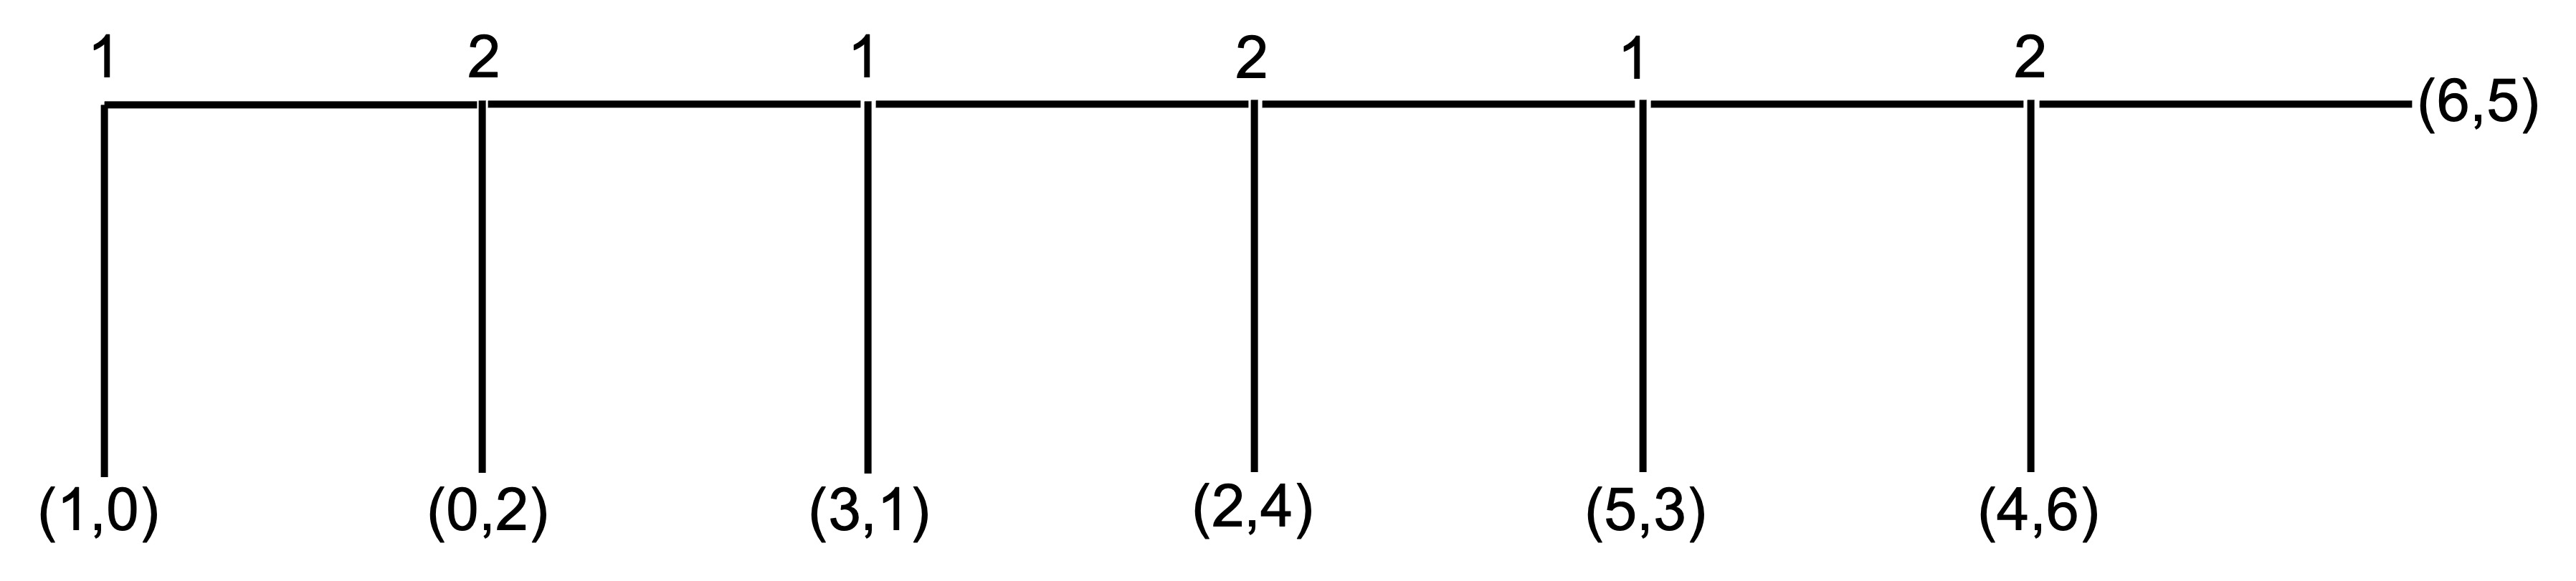
\includegraphics{behavioural-game-theory/img/centipede.jpg}

What do people do when playing the centipede game in the lab?

People tend to pass until a few stages before the end (depending on the
length of the centipede) and then take.

Can level-k thinking provide an insight into this behaviour?

Suppose a level-0 player passes until the end. They are possibly lucky
if they are player 1 playing against another level-0 player.

A level-1 player 2 would take at (4,6) as they know the level-0 player 1
would pass until then. A Level-1 player 1 would be planning to take
(6,5) at the end as they believe the level-0 player 2 will keep passing

A level-2 player 2 would plan to take at the final stage (4,6) as they
believe the level-1 player 1 pass. A level-2 player 1 would take the
payoff at (5,3) as they believe a level-1 player 2 would take at (4,6).

A level-3 player 2 would plan to take at (2,4) as they believe the
level-1 player 1 will take at (5,3). A level-3 player 1 would plan to
take at (5,3) as they believe a level-2 player 2 would take at (4,6).

And so on.

\hypertarget{asymmetric-information-1}{%
\chapter{Asymmetric information}\label{asymmetric-information-1}}

We saw earlier in our examination of the market for lemons and the
winner's curse that asymmetric information can cause market failures
even if agents are fully rational.

When we mix psychology and asymmetric information:

\begin{itemize}
\item
  People under-estimate the extent to which informational differences
  drive others' behaviour. They often act as if others have the same
  information set that they do
\item
  Better informed agents can fail to take advantage of their
  informational advantage against less informed agents because they
  don't understand the link between information and behaviour.
\end{itemize}

We will examine a phenomenon, the curse of knowledge, where agents with
a different information set under-appreciate the extent to which others'
strategies depend on that information.

\hypertarget{the-curse-of-knowledge}{%
\section{The curse of knowledge}\label{the-curse-of-knowledge}}

The idea behind the curse of knowledge is that better informed agents
should ignore the additional information they hold when predicting the
actions of less-informed agents. Experimental evidence shows that people
are unable to ignore their private information even when it is in their
interests to do so.

For example, Newton (1990) had students participated in an experiment in
one of two roles: ``Tapper'' and ``Listener''.

Tappers received a list of 25 well-known songs and were asked to ``tap
out'' the rhythm of one of the songs.

Listeners tried to identify the song based solely on the taps.

Tappers predicted that listeners would identify 50\% of the songs.

Listeners only identified 3 of 120 songs correctly (a rate of about
2.5\%).

\hypertarget{cursed-equilibrium}{%
\section{Cursed equilibrium}\label{cursed-equilibrium}}

Eyster and Rabin (2005) developed a model of ``cursed equilibrium''.

A cursed player underestimates the extent to which another player's
behaviour depends on that player's private information.

In the extreme case a fully-cursed player thinks the other player's
behaviour doesn't depend on their private information at all. A
fully-cursed player understands that the other player might do different
things (e.g.~bid high or low), but thinks that this is independent of
their private information.

They propose ``cursed equilibrium'', where each player correctly
anticipates the distribution of play by others and maximizes utility
given their (cursed) beliefs.

That is, cursed players do not fully take into account the correlation
between the actions of other players and their types. Instead, cursed
players believe their opponent plays the average optimal action, not the
type-contingent action.

\hypertarget{the-market-for-lemons-1}{%
\subsection{The market for lemons}\label{the-market-for-lemons-1}}

In the lemon market, a cursed buyer doesn't think that the seller's
decision of whether to say yes to the trade depends on the seller'
evaluation of the car.

Return to our market for lemons and suppose that \(q=0.2\). That is,
only 20\% of the cars are good. Under the parameters we explored, only
lemons are sold.

Rather than considering that the 20\% of good car owners are willing to
sell their car with 0\% probability and the 80\% of lemon owners are
willing to sell with 100\% probability, the cursed players might average
over the two types and consider each type has an 80\% chance to sell.

Under that miscalculation they are willing to pay up to the (mistakenly)
expected value of:

\[
E=0.8×15000+0.2×7500=13500
\]

They would be willing to pay up to \$13,500 despite the market
comprising only lemons (valued at only \$7,500 by buyers).

\hypertarget{the-winners-curse-1}{%
\section{The winner's curse}\label{the-winners-curse-1}}

Consider now our example of the winner's curse and bidding for an oil
field.

Assume Player 1 is fully cursed and therefore assumes Player 2's bid is
independent of \(v_2\). Player 1 assumes \(v_2\) is on average \$50 and
that Player 2 bids half of the time regardless of \(v_2\).

Company 1's expected profit if they bid \(v_1\) is:

\begin{align*}
\hat E[\pi_1|\text{bid }v_1]&=\frac{1}{2}\pi_1(2\text{ no bid}|v_2=50)+\frac{1}{2}\bigg(\frac{1}{2}\pi_1(\text{lose}|v_2=50)+\frac{1}{2}\pi_1(\text{win}|v_2=50)\bigg) \\
&=\frac{1}{2}\bigg(\frac{v_1+50}{2}-v_1\bigg)+\frac{1}{4}\times 0+\frac{1}{4}\bigg(\frac{v_1+50}{2}-v_1\bigg) \\
&=\frac{3}{4}(25-\frac{v_1}{2})
\end{align*}

We can see that:

\[
\hat E[\pi_1|\text{bid}]>0 \Leftrightarrow v_1>50
\]

However, as shown previously, this bidding approach leads to an expected
loss.

In general, the cursed bidder under-appreciates that another bidder is
more likely not to bid when that other bidder's information is bad.
Therefore, they under-appreciate the extent to which winning the auction
is bad news.

\hypertarget{emotions}{%
\chapter{Emotions}\label{emotions}}

Emotions are mental states that signal positive or negative outcomes.

It is possible that one function of emotions is to act as a commitment
device:

\begin{itemize}
\item
  The emotion of guilt can constrain a desire to ``cheat'' where
  cheating delivers a higher pay-off. This in turn may allow people to
  trust you.
\item
  The emotion of anger may lead you to punish someone even where
  delivering the punishment also harms you. This in turn may lead people
  to be less likely to cheat you.
\end{itemize}

While this behaviour may appear ``irrational'', it allows people to make
credible commitments that in turn allow them to enter beneficial trades
and cooperative arrangements, while being less likely to being cheated.

\hypertarget{commitment-1}{%
\section{Commitment}\label{commitment-1}}

Recall our earlier example of a customer threatening to complain if they
receive bad service.

\includegraphics{behavioural-game-theory/img/complain-2.jpg}

What if the customer gets a strong sense of satisfaction from
complaining worth +3? Then their payoffs become as follows:

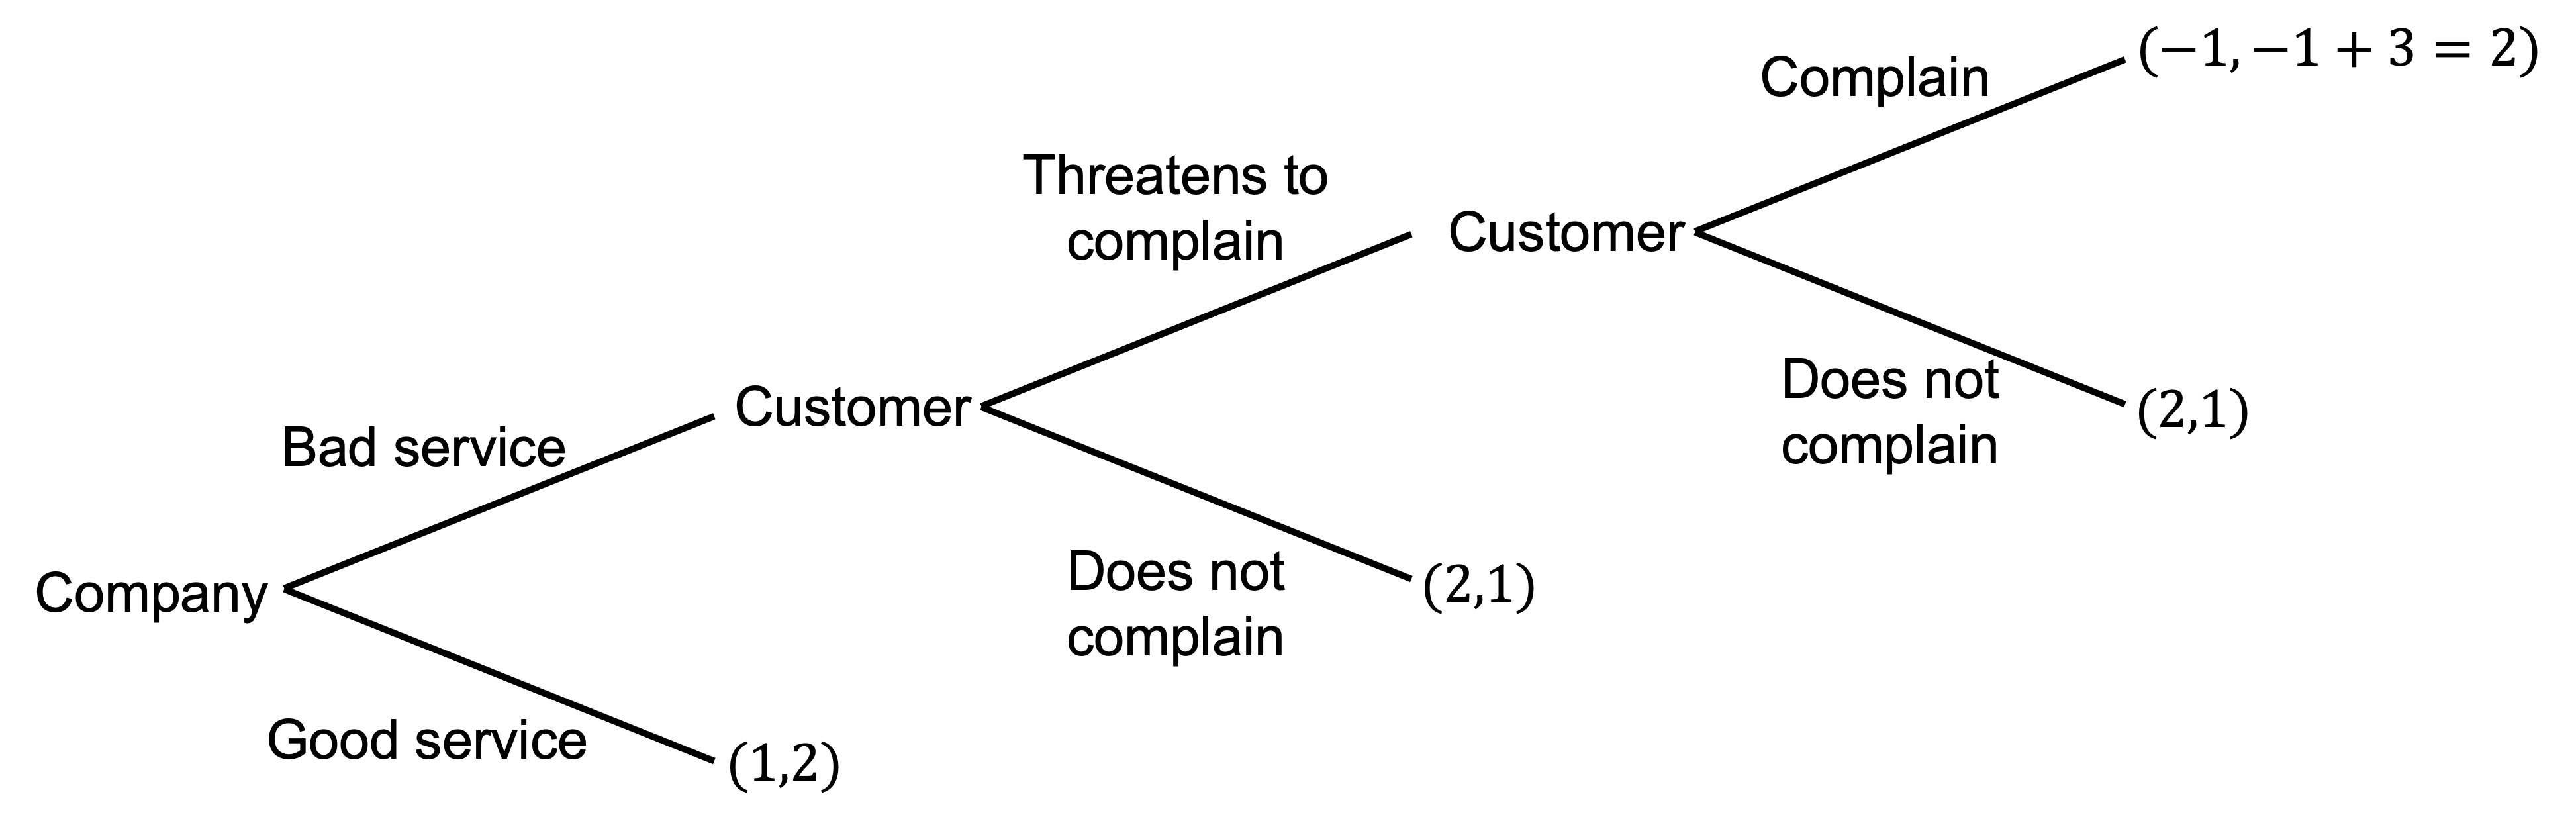
\includegraphics{behavioural-game-theory/img/complain-3.jpg}

The threat to complain is now credible. The company now provides good
service.

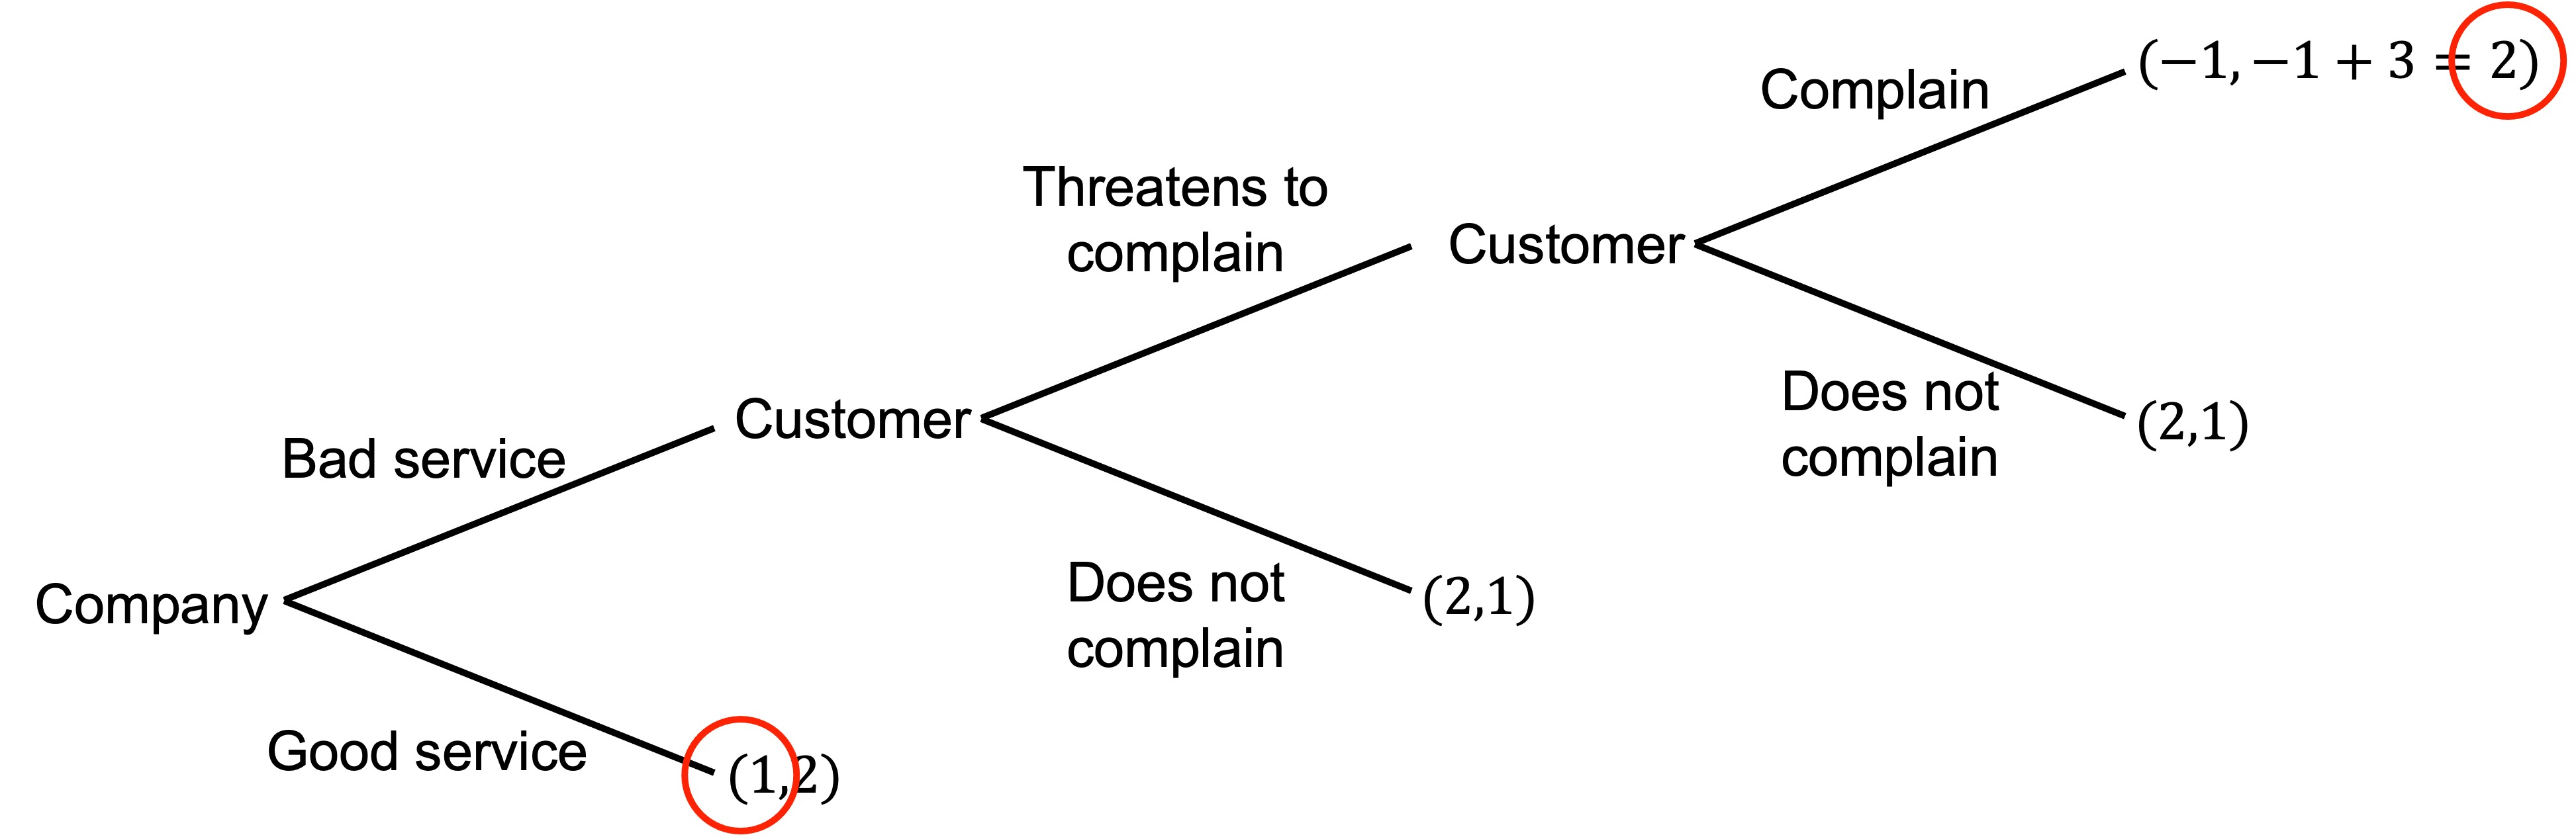
\includegraphics{behavioural-game-theory/img/complain-4.jpg}

\hypertarget{chicken-1}{%
\section{Chicken}\label{chicken-1}}

Recall the game of chicken.

\includegraphics{behavioural-game-theory/img/chicken-1.jpg}

Player A is crazy. They are afraid of nothing and will never swerve.
Player B knows this.

Player A's craziness acts as a commitment device similar to that of
removing the Steering Wheel. If Player A will not swerve, Player B will.

\includegraphics{behavioural-game-theory/img/chicken-3.jpg}

\hypertarget{behavioural-game-theory-exercises}{%
\chapter{Behavioural game theory
exercises}\label{behavioural-game-theory-exercises}}

\hypertarget{penalty-kick}{%
\section{Penalty kick}\label{penalty-kick}}

A soccer player (the striker) has a penalty kick. The striker is
deciding whether to kick to the left or right. If the goalkeeper dives
in the correct direction, the goalkeeper will stop the ball and the two
sides will tie. Otherwise, the striker will score a goal and win.

Lately, the striker has been having trouble kicking to the right,
sometimes missing the goals even when the goalkeeper doesn't dive in
that direction.

The expected payoffs for each combination of actions are as follows,
with the payoff (\(x,y\)) being the payoffs for the striker and
goalkeeper respectively:

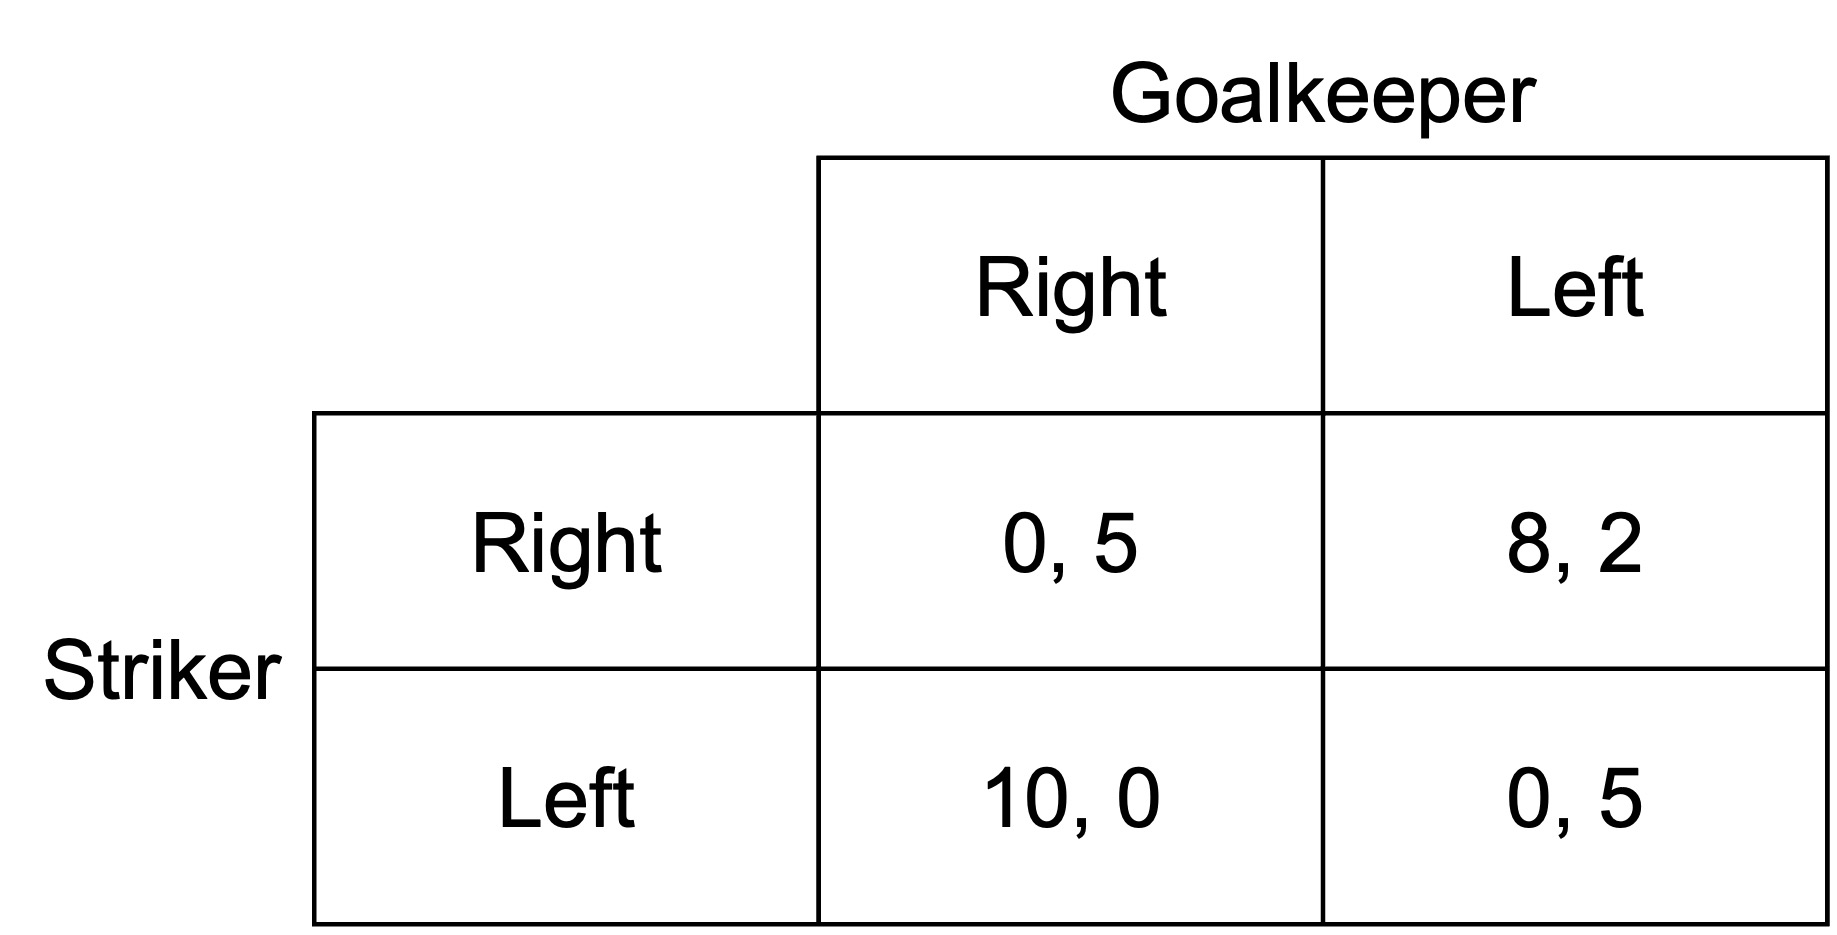
\includegraphics[width=0.6\textwidth,height=\textheight]{behavioural-game-theory/img/soccer.jpg}

Are there any pure-strategy Nash equilibria? If so, what are they?

There are no pure-strategy Nash equilibria. Whatever the striker does,
the goalkeeper wants to match. If the goalkeeper matches, the striker
wants to change.

a) Suppose the striker and goalkeeper are level-k thinkers.

If they were level-0, both would choose right or left with equal
probability.

What would each player do if they were a level-1 thinker? Explain.

\begin{tcolorbox}[enhanced jigsaw, title=\textcolor{quarto-callout-tip-color}{\faLightbulb}\hspace{0.5em}{Answer}, toprule=.15mm, colback=white, breakable, titlerule=0mm, colframe=quarto-callout-tip-color-frame, coltitle=black, opacityback=0, rightrule=.15mm, colbacktitle=quarto-callout-tip-color!10!white, bottomtitle=1mm, opacitybacktitle=0.6, arc=.35mm, bottomrule=.15mm, toptitle=1mm, leftrule=.75mm, left=2mm]

A level-1 striker will assume they are playing a level-0 goalkeeper.

They will estimate the the payoff from each action responding to the
random play of a level-0 goalkeeper.

\begin{align*}
E[U_S(R)]&=0.5\times 0+0.5\times 8 \\
&=4 \\
\\
E[U_S(L)]&=0.5\times 10+0.5*\times 0 \\
&=5
\end{align*}

The level-1 striker has a higher expected payoff for kicking left, so
kick left.

A level-1 goalkeeper will assume they are playing a level-0 striker.

They will estimate the the payoff from each action responding to the
random play of a level-0 striker.

\begin{align*}
E[U_G(R)]&=0.5\times 5+0.5\times 0 \\
&=2.5 \\
\\
E[U_G(L)]&=0.5\times 2+0.5*\times 5 \\
&=3.5
\end{align*}

The level-1 goalkeeper has a higher expected payoff for going left, so
go left.

\end{tcolorbox}

b) What would each player do if they were a level-2 thinker? Explain.

\begin{tcolorbox}[enhanced jigsaw, title=\textcolor{quarto-callout-tip-color}{\faLightbulb}\hspace{0.5em}{Answer}, toprule=.15mm, colback=white, breakable, titlerule=0mm, colframe=quarto-callout-tip-color-frame, coltitle=black, opacityback=0, rightrule=.15mm, colbacktitle=quarto-callout-tip-color!10!white, bottomtitle=1mm, opacitybacktitle=0.6, arc=.35mm, bottomrule=.15mm, toptitle=1mm, leftrule=.75mm, left=2mm]

A level-2 striker will assume they are playing a level-1 goalkeeper.

They believe the level-1 goalkeeper will go left, so they will go right
(payoff 8 compared to payoff 0).

A level-2 goalkeeper will assume they are playing a level-1 striker.

They believe the level-1 striker will go left, so they will go left
(payoff 5 compared to payoff 0).

\end{tcolorbox}

\hypertarget{hide-and-seek}{%
\section{Hide and seek}\label{hide-and-seek}}

In the hide-and-seek game, the Hider selects one of the four boxes
marked A, B, A and A. The Seeker guesses the box selected by the hider.

The Seeker wins if they find the Hider. Otherwise, the Hider wins.


\includegraphics[width=0.8\textwidth,height=\textheight]{behavioural-game-theory/img/hide-and-seek-1.jpg}

The payoffs are as follows. I have labelled the end boxes A1 and A2 to
distinguish the ``A''s from each other.

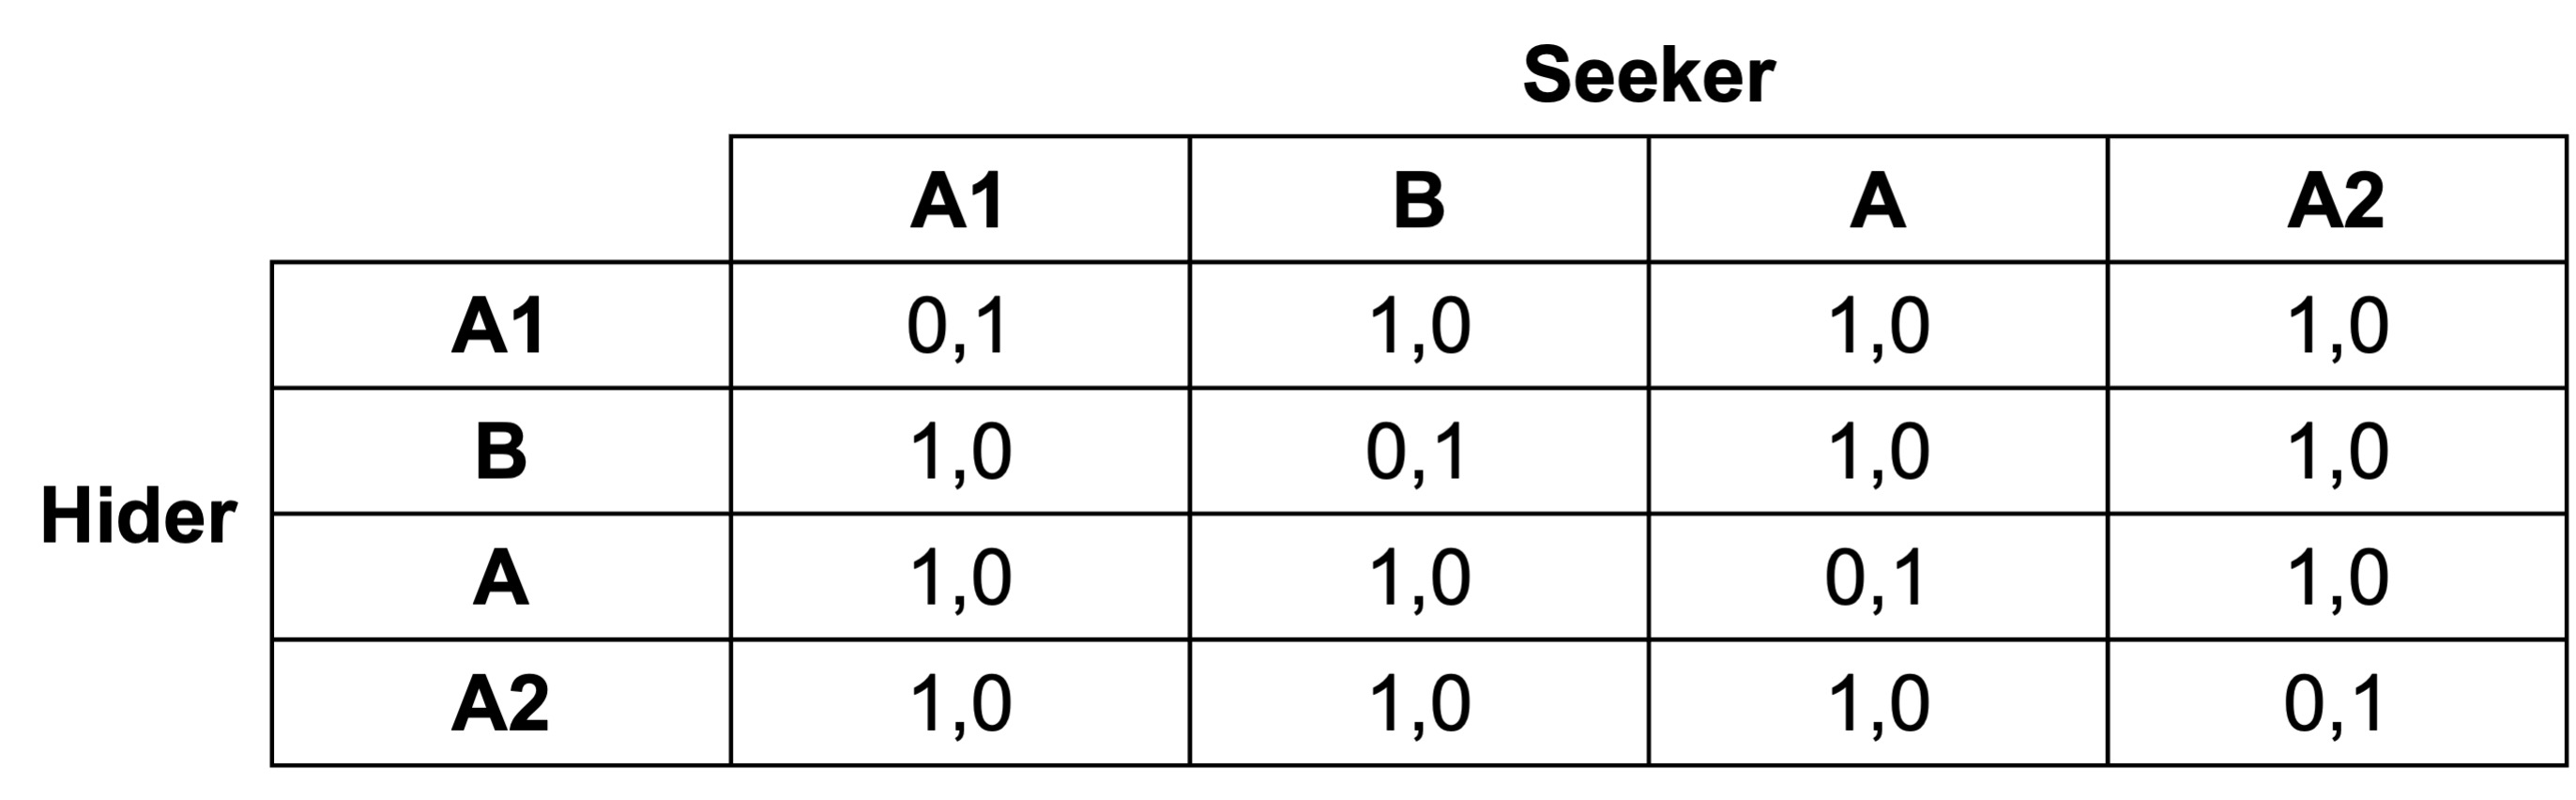
\includegraphics{behavioural-game-theory/img/hide-and-seek-2.jpg}

Assume a level-0 seeker or hider selects a box by hiding in or looking
in the ``most salient'' hiding spots. They choose A1 or A2 on the ends
with \(p=0.3\) each, or B (because it is different) with \(p=0.35\).
They hide or look in less salient middle A with probability
\(1−2\times 0.3−0.35=0.05\).

(Note that this assumption for the level-0 agents is different to what
we have assumed to date. We have typically assumed a level-0 agent
randomly chooses an action.)

a) What box do the level-1 hider and seeker choose?

\begin{tcolorbox}[enhanced jigsaw, title=\textcolor{quarto-callout-tip-color}{\faLightbulb}\hspace{0.5em}{Answer}, toprule=.15mm, colback=white, breakable, titlerule=0mm, colframe=quarto-callout-tip-color-frame, coltitle=black, opacityback=0, rightrule=.15mm, colbacktitle=quarto-callout-tip-color!10!white, bottomtitle=1mm, opacitybacktitle=0.6, arc=.35mm, bottomrule=.15mm, toptitle=1mm, leftrule=.75mm, left=2mm]

The level-1 hider calculates the expected payoff from hiding in each of
the boxes if playing against a level-0 seeker.

\begin{align*}
E[U(A1)]&=0×0.3+1×0.35+1×0.05+1×0.3=0.7 \\
\\
E[U(B)]&=1×0.3+0×0.35+1×0.05+1×0.3=0.65 \\
\\
E[U(A)]&=1×0.3+1×0.35+0×0.05+1×0.3=0.95 \\
\\
E[U(A2)]&=1×0.3+1×0.35+1×0.05+0×0.3=0.7
\end{align*}

The level-1 hider hides in the least salient box A.

The level-1 seeker calculates the expected payoff from looking in each
of the boxes if playing against a level-0 hider.

\begin{align*}
E[U(A1)]&=1×0.3+0×0.35+0×0.05+0×0.3=0.3 \\
\\
E[U(B)]&=0×0.3+1×0.35+0×0.05+0×0.3=0.35 \\
\\
E[U(A)]&=0×0.3+0×0.35+1×0.05+0×0.3=0.05 \\
\\
E[U(A2)]&=0×0.3+0×0.35+0×0.05+1×0.3=0.3
\end{align*}

The level-1 seeker looks in Box B.

If both the hider and seeker are level-1, the hider wins.

\end{tcolorbox}

b) What box do the level-2 hider and seeker choose?

\begin{tcolorbox}[enhanced jigsaw, title=\textcolor{quarto-callout-tip-color}{\faLightbulb}\hspace{0.5em}{Answer}, toprule=.15mm, colback=white, breakable, titlerule=0mm, colframe=quarto-callout-tip-color-frame, coltitle=black, opacityback=0, rightrule=.15mm, colbacktitle=quarto-callout-tip-color!10!white, bottomtitle=1mm, opacitybacktitle=0.6, arc=.35mm, bottomrule=.15mm, toptitle=1mm, leftrule=.75mm, left=2mm]

The level-2 hider knows that the level-1 seeker chooses B. They select
any box apart from B with equal probability, all of which they believe
will give a pay-off of 1.

The level-2 seeker knows that the level-1 hider will select A. They
select A.

The level-2 seeker wins with probability \(1/3\).

\end{tcolorbox}

c) What box do the level-3 hider and seeker choose?

\begin{tcolorbox}[enhanced jigsaw, title=\textcolor{quarto-callout-tip-color}{\faLightbulb}\hspace{0.5em}{Answer}, toprule=.15mm, colback=white, breakable, titlerule=0mm, colframe=quarto-callout-tip-color-frame, coltitle=black, opacityback=0, rightrule=.15mm, colbacktitle=quarto-callout-tip-color!10!white, bottomtitle=1mm, opacitybacktitle=0.6, arc=.35mm, bottomrule=.15mm, toptitle=1mm, leftrule=.75mm, left=2mm]

The level-3 hider knows that the level-2 seeker chooses A. They select
any box apart from A with equal probability, all of which they believe
will give a pay-off of 1.

The level-3 seeker knows that the level-2 hider will select any box
except B with equal probability. They select one of A1, A2 or A with
equal probability.

The level-3 seeker wins with probability \(1/3×1/3+1/3×1/3=2/9\).

\end{tcolorbox}

d) What box do the level-4 hider and seeker choose?

\begin{tcolorbox}[enhanced jigsaw, title=\textcolor{quarto-callout-tip-color}{\faLightbulb}\hspace{0.5em}{Answer}, toprule=.15mm, colback=white, breakable, titlerule=0mm, colframe=quarto-callout-tip-color-frame, coltitle=black, opacityback=0, rightrule=.15mm, colbacktitle=quarto-callout-tip-color!10!white, bottomtitle=1mm, opacitybacktitle=0.6, arc=.35mm, bottomrule=.15mm, toptitle=1mm, leftrule=.75mm, left=2mm]

The level-4 hider knows that the level-3 seeker selected A1, A2 and A
with equal probability. They select B.

The level-4 seeker knows that the level-3 hider selected any box apart
from A with equal probability. They also select those boxes with equal
probability.

The level-4 seeker wins with probability \(1/3\).

\end{tcolorbox}

\hypertarget{matching-pennies-with-a-twist}{%
\section{Matching pennies (with a
twist)}\label{matching-pennies-with-a-twist}}

Consider the following two-player game:

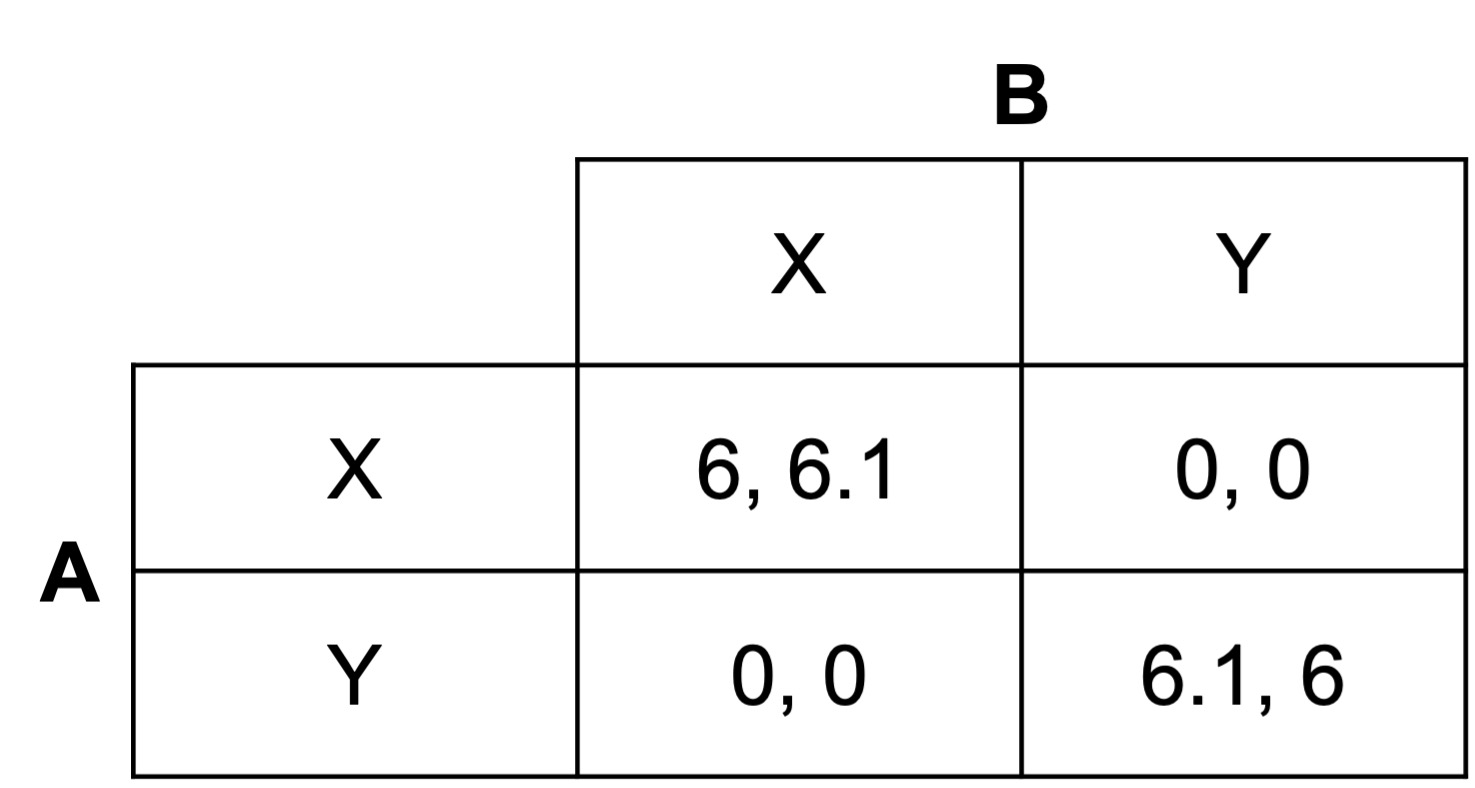
\includegraphics[width=0.6\textwidth,height=\textheight]{behavioural-game-theory/img/matching.jpg}

a) What are the two pure-strategy Nash equilibria of this game?

\begin{tcolorbox}[enhanced jigsaw, title=\textcolor{quarto-callout-tip-color}{\faLightbulb}\hspace{0.5em}{Answer}, toprule=.15mm, colback=white, breakable, titlerule=0mm, colframe=quarto-callout-tip-color-frame, coltitle=black, opacityback=0, rightrule=.15mm, colbacktitle=quarto-callout-tip-color!10!white, bottomtitle=1mm, opacitybacktitle=0.6, arc=.35mm, bottomrule=.15mm, toptitle=1mm, leftrule=.75mm, left=2mm]

The two pure-strategy Nash equilibria of this game are (X,X) and (Y,Y).
That is, if the players are jointly playing either of those combinations
of strategies, neither has an incentive to deviate. Their response is a
best response to the other players' actions.

\end{tcolorbox}

b) Suppose players in this game think according to the level-k model.
Assume a level-0 agent randomises between options with equal
probability.

What would player A and player B do if they were level-1 players?

\begin{tcolorbox}[enhanced jigsaw, title=\textcolor{quarto-callout-tip-color}{\faLightbulb}\hspace{0.5em}{Answer}, toprule=.15mm, colback=white, breakable, titlerule=0mm, colframe=quarto-callout-tip-color-frame, coltitle=black, opacityback=0, rightrule=.15mm, colbacktitle=quarto-callout-tip-color!10!white, bottomtitle=1mm, opacitybacktitle=0.6, arc=.35mm, bottomrule=.15mm, toptitle=1mm, leftrule=.75mm, left=2mm]

Remember the idea behind level-k thinking: given their own cognitive
level, a player forms an expectation of what others will do and tries to
be ``one step ahead of them''.

We work out the utility of each option.

First, for player A:

\begin{align*}
EU ^{1}_{A}(X)&= 0.5\times 6+0.5\times 0=3 \\
\\
EU ^{1}_{A}(Y)&= 0.5\times 0+0.5\times 6.1=3.05
\end{align*}

Player A chooses Y if they are a level-1 player.

Next, for player B:

\begin{align*}
EU ^{1}_{B}(X)&= 0.5\times 6.1+0.5\times 0=3.05 \\
\\
EU ^{1}_{B}(Y)&= 0.5\times 0+0.5\times 6=3
\end{align*}

Player B chooses X if they are a level-1 player.

If both players are level-1, they will fail to coordinate.

\end{tcolorbox}

c) What would player A and player B do if they were level-2 players?

\begin{tcolorbox}[enhanced jigsaw, title=\textcolor{quarto-callout-tip-color}{\faLightbulb}\hspace{0.5em}{Answer}, toprule=.15mm, colback=white, breakable, titlerule=0mm, colframe=quarto-callout-tip-color-frame, coltitle=black, opacityback=0, rightrule=.15mm, colbacktitle=quarto-callout-tip-color!10!white, bottomtitle=1mm, opacitybacktitle=0.6, arc=.35mm, bottomrule=.15mm, toptitle=1mm, leftrule=.75mm, left=2mm]

We again work out the utility of each option:

First, for player A. They know that a level-1 player B will select X.
Accordingly:

\begin{align*}
EU^{2}_{A}(X)&=1\times 6+0\times 0=6 \\
\\
EU^{2}_{A}(Y)&=1\times 0+0\times 6.1=0
\end{align*}

Player A chooses X if they are a level-2 player.

Next, for player B. They know that a level-1 player A will select Y.
Accordingly:

\begin{align*}
EU ^{2}_{B}(X)&= 0\times 6.1+1\times0=0 \\
\\
EU ^{2}_{B}(Y)&= 0\times 0+1\times 6=6
\end{align*}

Player B chooses Y if they are a level-2 player.

If both players are level-2, they will fail to coordinate.

\end{tcolorbox}

d) What would player A and player B do if they were level-3 players?

\begin{tcolorbox}[enhanced jigsaw, title=\textcolor{quarto-callout-tip-color}{\faLightbulb}\hspace{0.5em}{Answer}, toprule=.15mm, colback=white, breakable, titlerule=0mm, colframe=quarto-callout-tip-color-frame, coltitle=black, opacityback=0, rightrule=.15mm, colbacktitle=quarto-callout-tip-color!10!white, bottomtitle=1mm, opacitybacktitle=0.6, arc=.35mm, bottomrule=.15mm, toptitle=1mm, leftrule=.75mm, left=2mm]

We again work out the utility of each option:

First, for player A. They know that a level-2 player B will select Y.
Accordingly:

\begin{align*}
EU ^{3}_{A}(X)&= 0\times 6+1\times 0=0 \\
\\
EU ^{3}_{A}(Y)&= 0\times 0+1\times 6.1=6.1
\end{align*}

Player A chooses Y if they are a level-3 player.

Next, for player B. They know that a level-2 player A will select X.
Accordingly:

\begin{align*}
EU ^{3}_{B}(X)&= 1\times 6.1+0\times 0=6.1 \\
\\
EU ^{3}_{B}(Y)&= 1\times 0+0\times 6=0
\end{align*}

Player B chooses X if they are a level-3 player.

If both players are level-3, they will fail to coordinate.

\end{tcolorbox}

e) When this game is played in the laboratory, the players
mis-coordinate. About 3/4 of the row players (player A) choose X while
about 3/4 of the column players (player B) choose Y.

Of interest, each player tries to coordinate on the strategy that the
other player would be better off coordinating on. That is, Player A
receives 6 from successful coordination choosing X, which is less than
the 6.1 Player A would get from coordinating on Y.

Given your answers to b) through d), what mix of level-k players might
explain the mis-coordination described above?

\begin{tcolorbox}[enhanced jigsaw, title=\textcolor{quarto-callout-tip-color}{\faLightbulb}\hspace{0.5em}{Answer}, toprule=.15mm, colback=white, breakable, titlerule=0mm, colframe=quarto-callout-tip-color-frame, coltitle=black, opacityback=0, rightrule=.15mm, colbacktitle=quarto-callout-tip-color!10!white, bottomtitle=1mm, opacitybacktitle=0.6, arc=.35mm, bottomrule=.15mm, toptitle=1mm, leftrule=.75mm, left=2mm]

That 3/4 of Player ``A''s choose X and 3/4 of Player ``B''s choose Y
suggests there are many level-2 players (or possibly level-4). They each
assume that the other player is level-1 and has picked the option with
the highest payoff for themselves. They are effectively trying to
coordinate with the other player by assuming that the other will seek
their highest paying option. However, if both do this, both receive
nothing.

\end{tcolorbox}

\hypertarget{cafe}{%
\section{Cafe}\label{cafe}}

Two friends, Player 1 and Player 2, have arranged to meet at a cafe.
Neither can remember which of the two cafes in town they had arranged to
meet at.

Each player has a favourite cafe. However, they would prefer to go to
their less-favourite cafe with a friend than go to their favourite cafe
alone.

Each chooses a cafe and goes there. The payoffs for each combination of
choices are in the table below, with the payoffs \((x, y)\) being the
payoffs for Player 1 and Player 2 respectively.

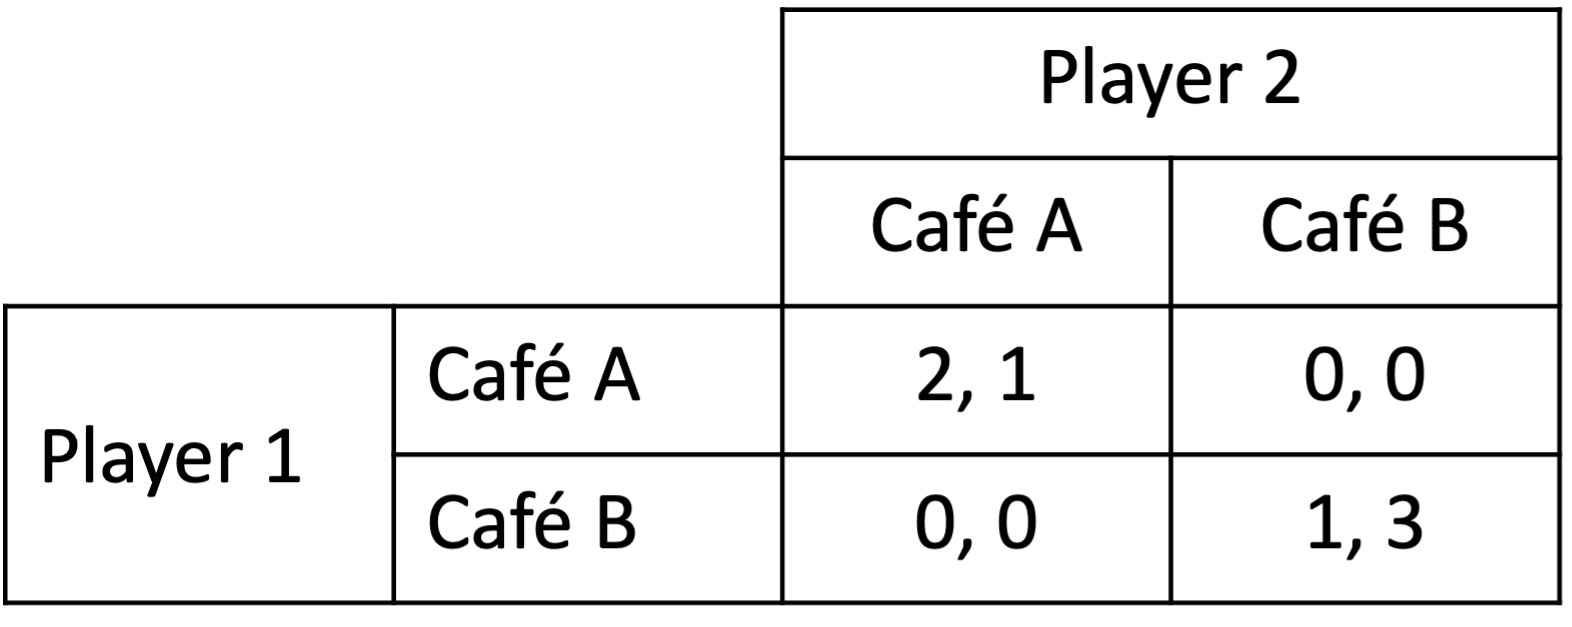
\includegraphics[width=0.6\textwidth,height=\textheight]{behavioural-game-theory/img/cafe-1.jpg}

a) What are the pure-strategy Nash equilbria of this game?

\begin{tcolorbox}[enhanced jigsaw, title=\textcolor{quarto-callout-tip-color}{\faLightbulb}\hspace{0.5em}{Answer}, toprule=.15mm, colback=white, breakable, titlerule=0mm, colframe=quarto-callout-tip-color-frame, coltitle=black, opacityback=0, rightrule=.15mm, colbacktitle=quarto-callout-tip-color!10!white, bottomtitle=1mm, opacitybacktitle=0.6, arc=.35mm, bottomrule=.15mm, toptitle=1mm, leftrule=.75mm, left=2mm]

If player 2 chooses cafe A, player 1 wants to choose cafe A.

If player 2 chooses cafe B, player 1 wants to choose cafe B.

If player 1 chooses cafe A, player 1 wants to choose cafe A.

If player 1 chooses cafe B, player 1 wants to choose cafe B.

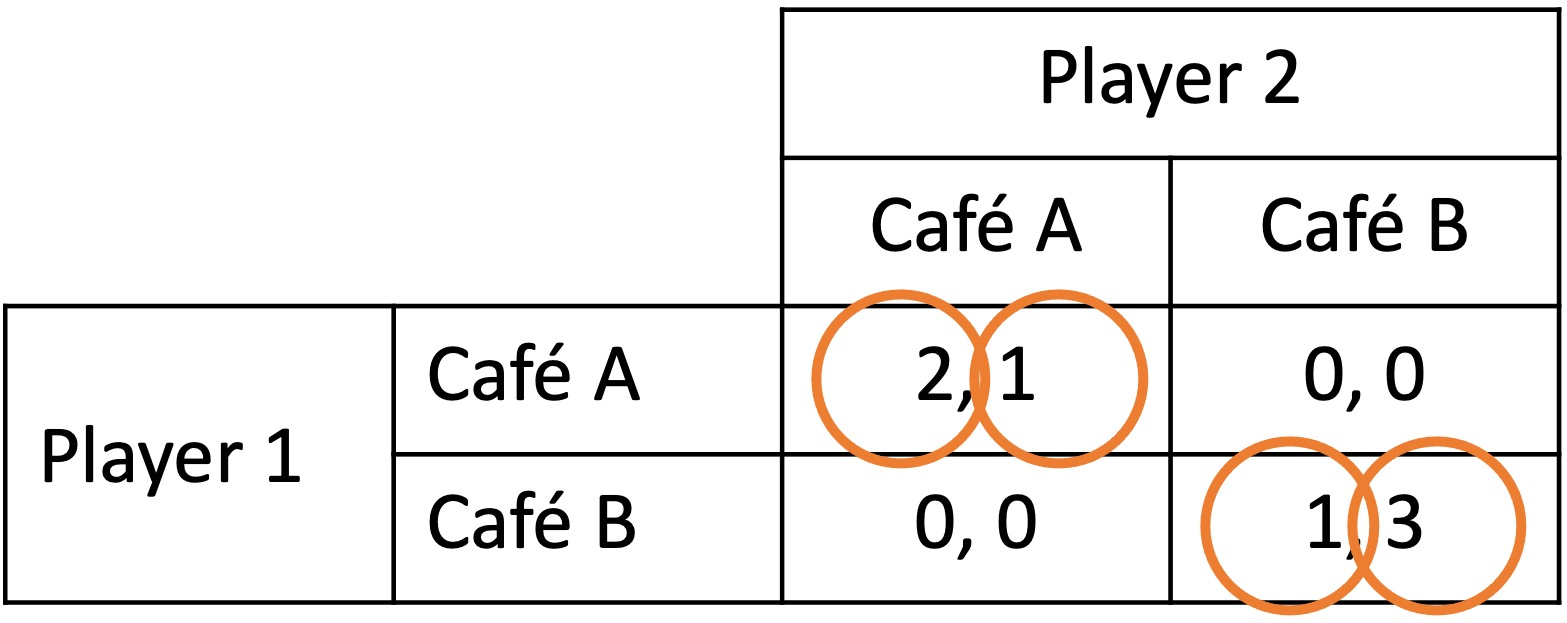
\includegraphics[width=0.6\textwidth,height=\textheight]{behavioural-game-theory/img/cafe-2.jpg}

The two pure-strategy Nash equilibria are (cafe A, cafe A) and (cafe B,
cafe B).

\end{tcolorbox}

b) What would Player 1 and Player 2 do if each was a level-1 thinker?
Explain.

\begin{tcolorbox}[enhanced jigsaw, title=\textcolor{quarto-callout-tip-color}{\faLightbulb}\hspace{0.5em}{Answer}, toprule=.15mm, colback=white, breakable, titlerule=0mm, colframe=quarto-callout-tip-color-frame, coltitle=black, opacityback=0, rightrule=.15mm, colbacktitle=quarto-callout-tip-color!10!white, bottomtitle=1mm, opacitybacktitle=0.6, arc=.35mm, bottomrule=.15mm, toptitle=1mm, leftrule=.75mm, left=2mm]

If Player 2 chooses randomly, Player 1's payoff's from each option are:

\begin{align*}
U_1(\text{cafe A})&=0.5\times 2+0.5\times 0=1 \\[6pt]
U_1(\text{cafe B})&=0.5\times 0+0.5\times 1=0.5
\end{align*}

Player 1 chooses cafe A.

If Player 1 chooses randomly, Player 2's payoff's from each option are:

\begin{align*}
U_2(\text{cafe A})&=0.5\times 1+0.5\times 0=0.5 \\[6pt]
U_2(\text{cafe B})&=0.5\times 0+0.5\times 3=1.5
\end{align*}

Player 2 chooses cafe B.

\end{tcolorbox}

c) What would Player 1 and Player 2 do if each was a level-2 thinker?
Explain.

\begin{tcolorbox}[enhanced jigsaw, title=\textcolor{quarto-callout-tip-color}{\faLightbulb}\hspace{0.5em}{Answer}, toprule=.15mm, colback=white, breakable, titlerule=0mm, colframe=quarto-callout-tip-color-frame, coltitle=black, opacityback=0, rightrule=.15mm, colbacktitle=quarto-callout-tip-color!10!white, bottomtitle=1mm, opacitybacktitle=0.6, arc=.35mm, bottomrule=.15mm, toptitle=1mm, leftrule=.75mm, left=2mm]

The level-2 Player 1 assumes that Player 2 is level-1. Therefore, they
assume that Player 2 will choose cafe B. Accordingly, they choose cafe
B.

The level-2 Player 2 assumes that Player 1 is level-1. Therefore, they
assume that Player 1 will choose cafe A. Accordingly, they choose cafe
A.

\end{tcolorbox}

\hypertarget{buying-a-car-1}{%
\section{Buying a car}\label{buying-a-car-1}}

Suppose that you are considering purchasing a car.

You believe that the seller values it between \$1000 and \$5000, with an
equal probability that it has a value at any point in this range. That
is, you believe it is uniformly valued to the seller between \$1000 and
\$5000.

The seller knows the car and its true value.

Assume that whatever the car is worth to the seller, it is worth 1.33
times that to you (so a car worth \$2400 to the owner is actually worth
\$3200 to you).

a) What offer should you make to ensure that you will not lose money?

\begin{tcolorbox}[enhanced jigsaw, title=\textcolor{quarto-callout-tip-color}{\faLightbulb}\hspace{0.5em}{Answer}, toprule=.15mm, colback=white, breakable, titlerule=0mm, colframe=quarto-callout-tip-color-frame, coltitle=black, opacityback=0, rightrule=.15mm, colbacktitle=quarto-callout-tip-color!10!white, bottomtitle=1mm, opacitybacktitle=0.6, arc=.35mm, bottomrule=.15mm, toptitle=1mm, leftrule=.75mm, left=2mm]

Suppose you offer \$\(x\). If the seller accepts, the value must be
between \$1000 and \$\(x\).

As the value evenly distributed across that interval, its average value
would be:

\[
1000+\frac{x−1000}{2}=500+\frac{x}{2}
\]

The expected value of the car to you will be:

\[
\frac{4}{3}\bigg(500+\frac{x}{2}\bigg)
\]

To ensure you don't lose you want:

\[
\frac{4}{3}\bigg(500+\frac{x}{2}\bigg)>x
\]

Solving this out, you expect to make a profit where \(x<\$2000\).

\end{tcolorbox}

b) Suppose you are cursed player and you believe sellers will take the
average optimal action of selling whenever they are offered more than
\$3000. As a result, you decide to offer \$3000. What is your accepted
profit if the seller accepts your offer?

\begin{tcolorbox}[enhanced jigsaw, title=\textcolor{quarto-callout-tip-color}{\faLightbulb}\hspace{0.5em}{Answer}, toprule=.15mm, colback=white, breakable, titlerule=0mm, colframe=quarto-callout-tip-color-frame, coltitle=black, opacityback=0, rightrule=.15mm, colbacktitle=quarto-callout-tip-color!10!white, bottomtitle=1mm, opacitybacktitle=0.6, arc=.35mm, bottomrule=.15mm, toptitle=1mm, leftrule=.75mm, left=2mm]

If seller accepts, the value must be between \$1000 and \$3000.

If value evenly distributed across that interval, its average value
would be \$2000.

Given it is worth 1.33 times more to you, it would be worth \$2,667 on
average.

You would lose, on average, \$333.

\end{tcolorbox}

\part{Social preferences}

\hypertarget{the-ultimatum-game-1}{%
\section*{The ultimatum game}\label{the-ultimatum-game-1}}
\addcontentsline{toc}{section}{The ultimatum game}

\markright{The ultimatum game}

Recall our earlier discussion of the ultimatum game.

\begin{quote}
The ultimatum game involves two players: the proposer and the responder.

The proposer is given a fixed amount of money \(m\). They then offer a
portion \(x\) of the sum \(m\) to the responder.

The responder can either accept of reject the offer. They make this
decision knowing \(m\) and \(x\). If the responder accepts, the
responder receives 𝑥 and the proposer gets \(m-x\). If the responder
rejects, both players receive nothing.
\end{quote}

Generally, if the players have monotonic preferences and the offer
strategy set is discrete:

\begin{itemize}
\item
  The responder accepts any \(x>0\).
\item
  The proposer offers \(x=\epsilon\), where \(\epsilon\) is the smallest
  non-zero amount the proposer can offer.
\end{itemize}

The other (weak) subgame perfect Nash equilibrium is an offer of \$0 and
acceptance.

What do people do in the ultimatum game?

Unlike the game theoretic predictions:

\begin{itemize}
\item
  Proposers rarely offer the minimum amount.
\item
  Responders often reject non-zero offers.
\end{itemize}

For example, Henrich et al. (2001) recruited subjects from 15
small-scale societies to play the ultimatum game. The mean offer is all
societies was substantially above zero. The rejection rate was low but
non-zero.

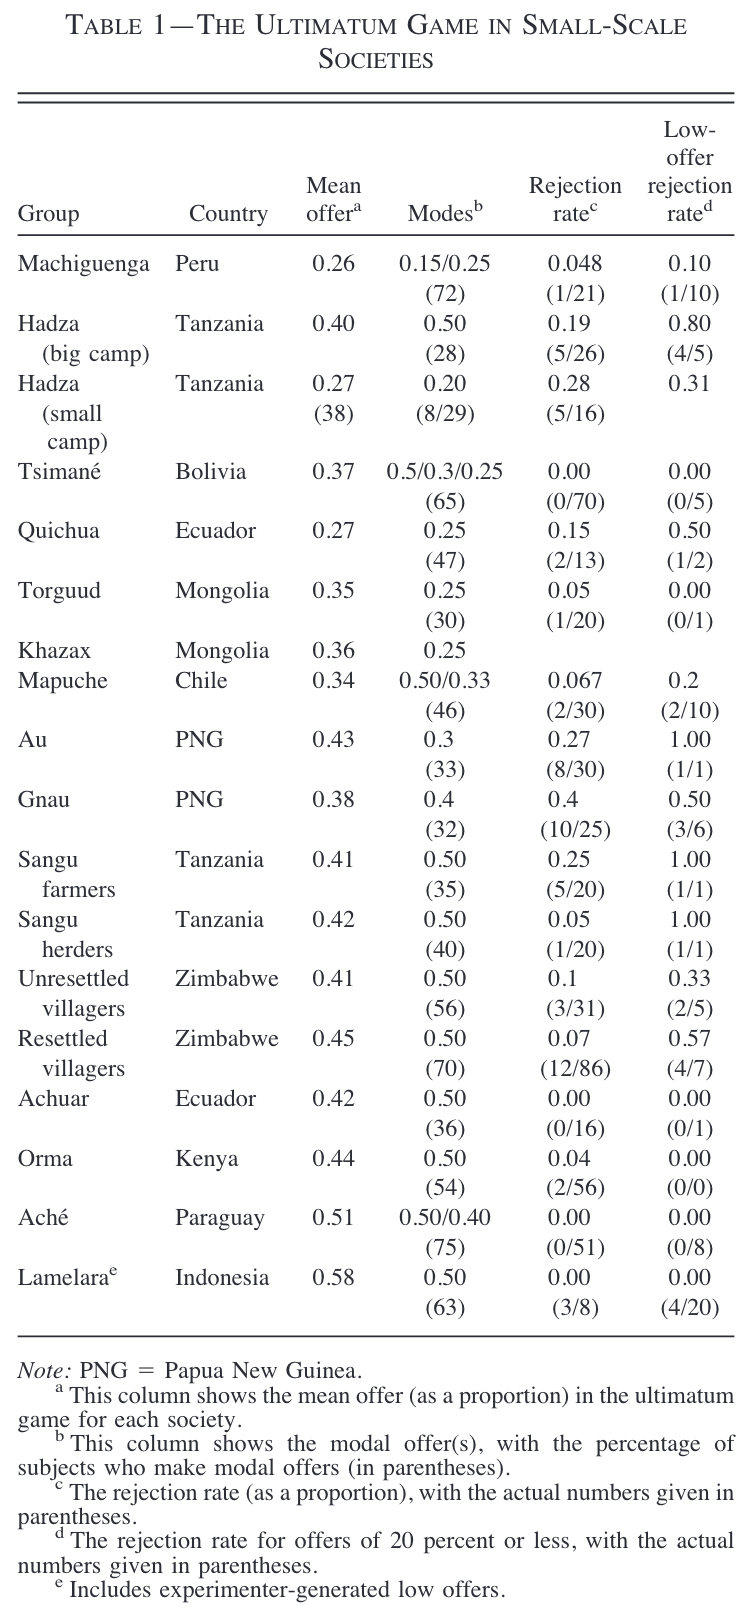
\includegraphics{social-preferences/img/henrich-2001-table-1.jpg}

\hypertarget{the-dictator-game-1}{%
\section*{The dictator game}\label{the-dictator-game-1}}
\addcontentsline{toc}{section}{The dictator game}

\markright{The dictator game}

Recall our earlier discussion of the dictator game.

\begin{quote}
In the dictator game, the dictator is given a fixed amount of money 𝑚.
They then offer a portion 𝑥 of the sum 𝑚 to the receiver. The game then
ends.

Exchange is unilateral. Receivers have an empty strategy set.
\end{quote}

The standard game theory prediction is no interaction.

However, in experiments dictators tend to give a positive sum of money.

\begin{figure}

\begin{minipage}[t]{0.50\linewidth}

{\centering 

\raisebox{-\height}{

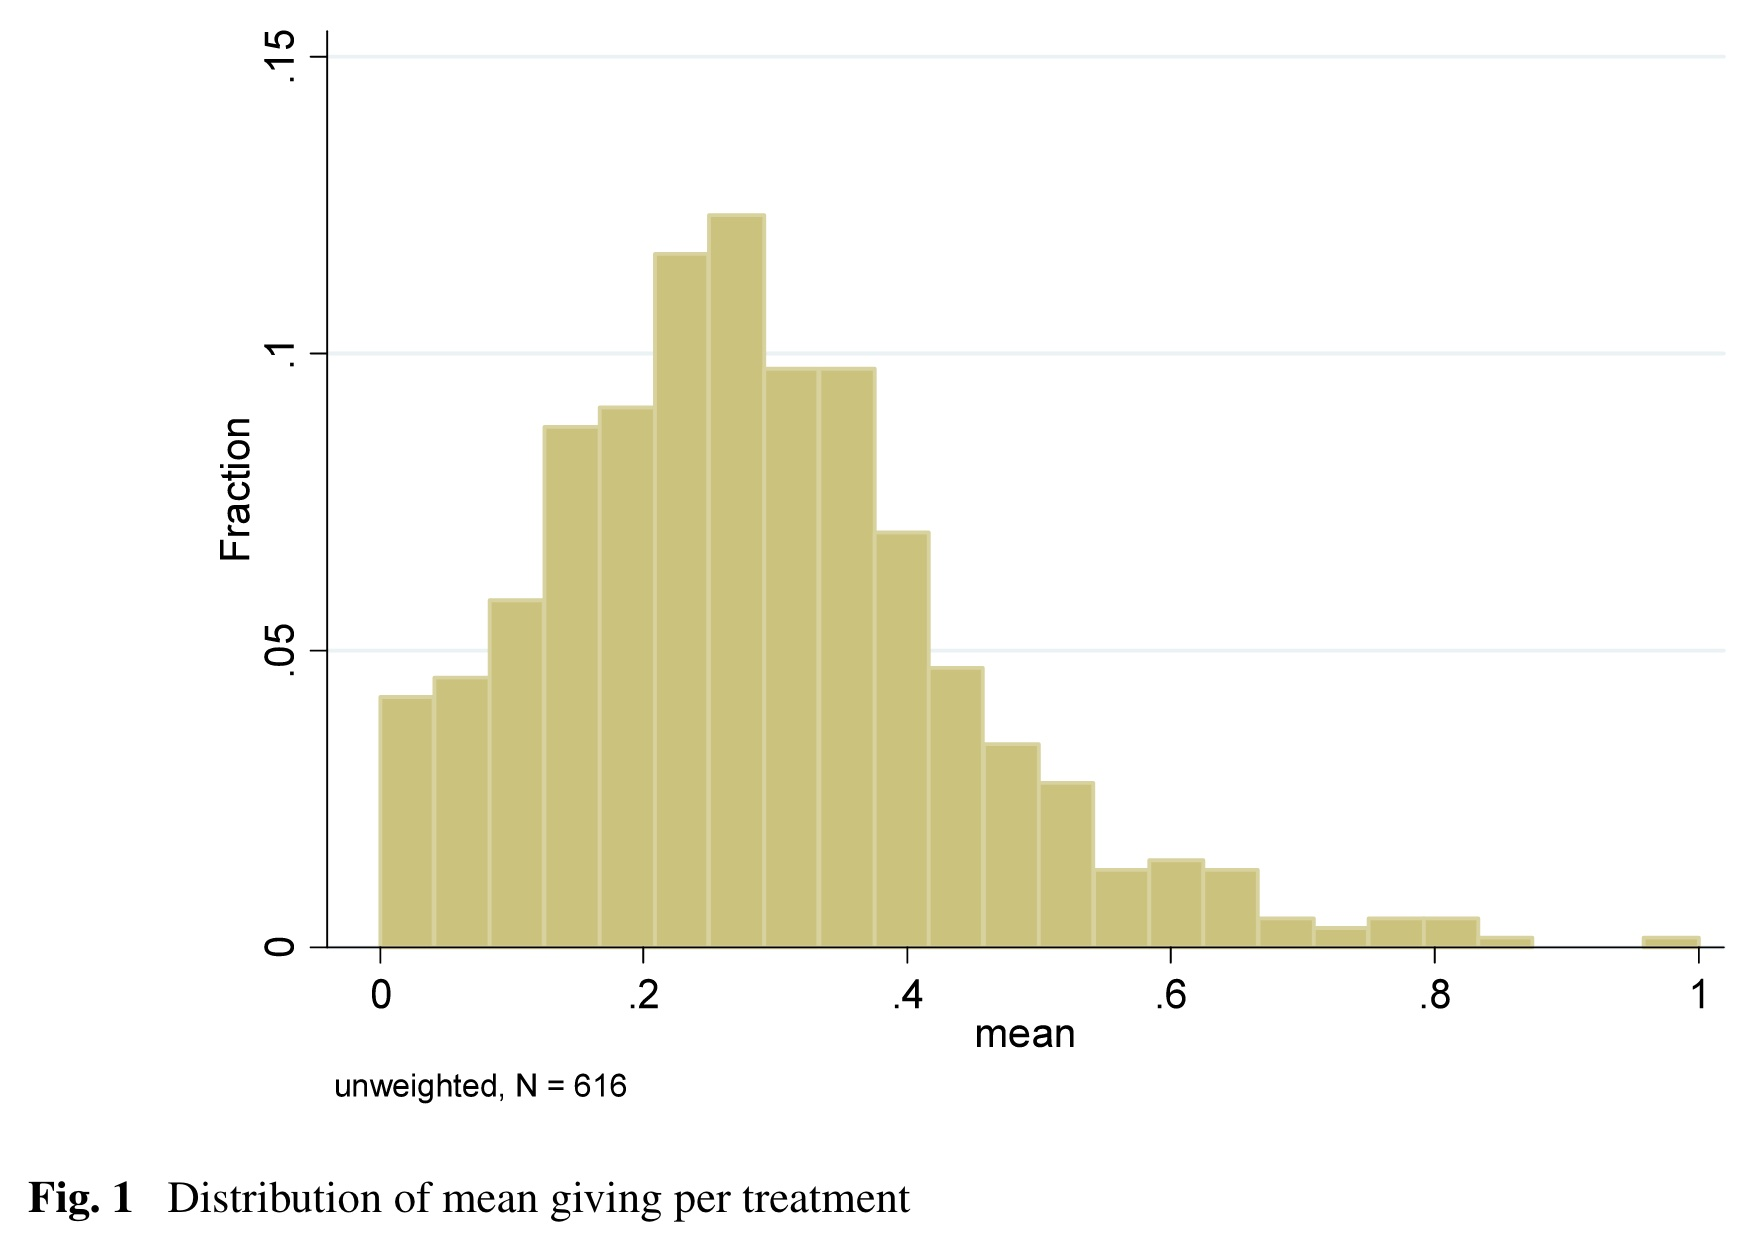
\includegraphics{social-preferences/img/engel-2011-fig-1.jpg}

}

}

\subcaption{\label{fig-engel1}Mean per treatment}
\end{minipage}%
%
\begin{minipage}[t]{0.50\linewidth}

{\centering 

\raisebox{-\height}{

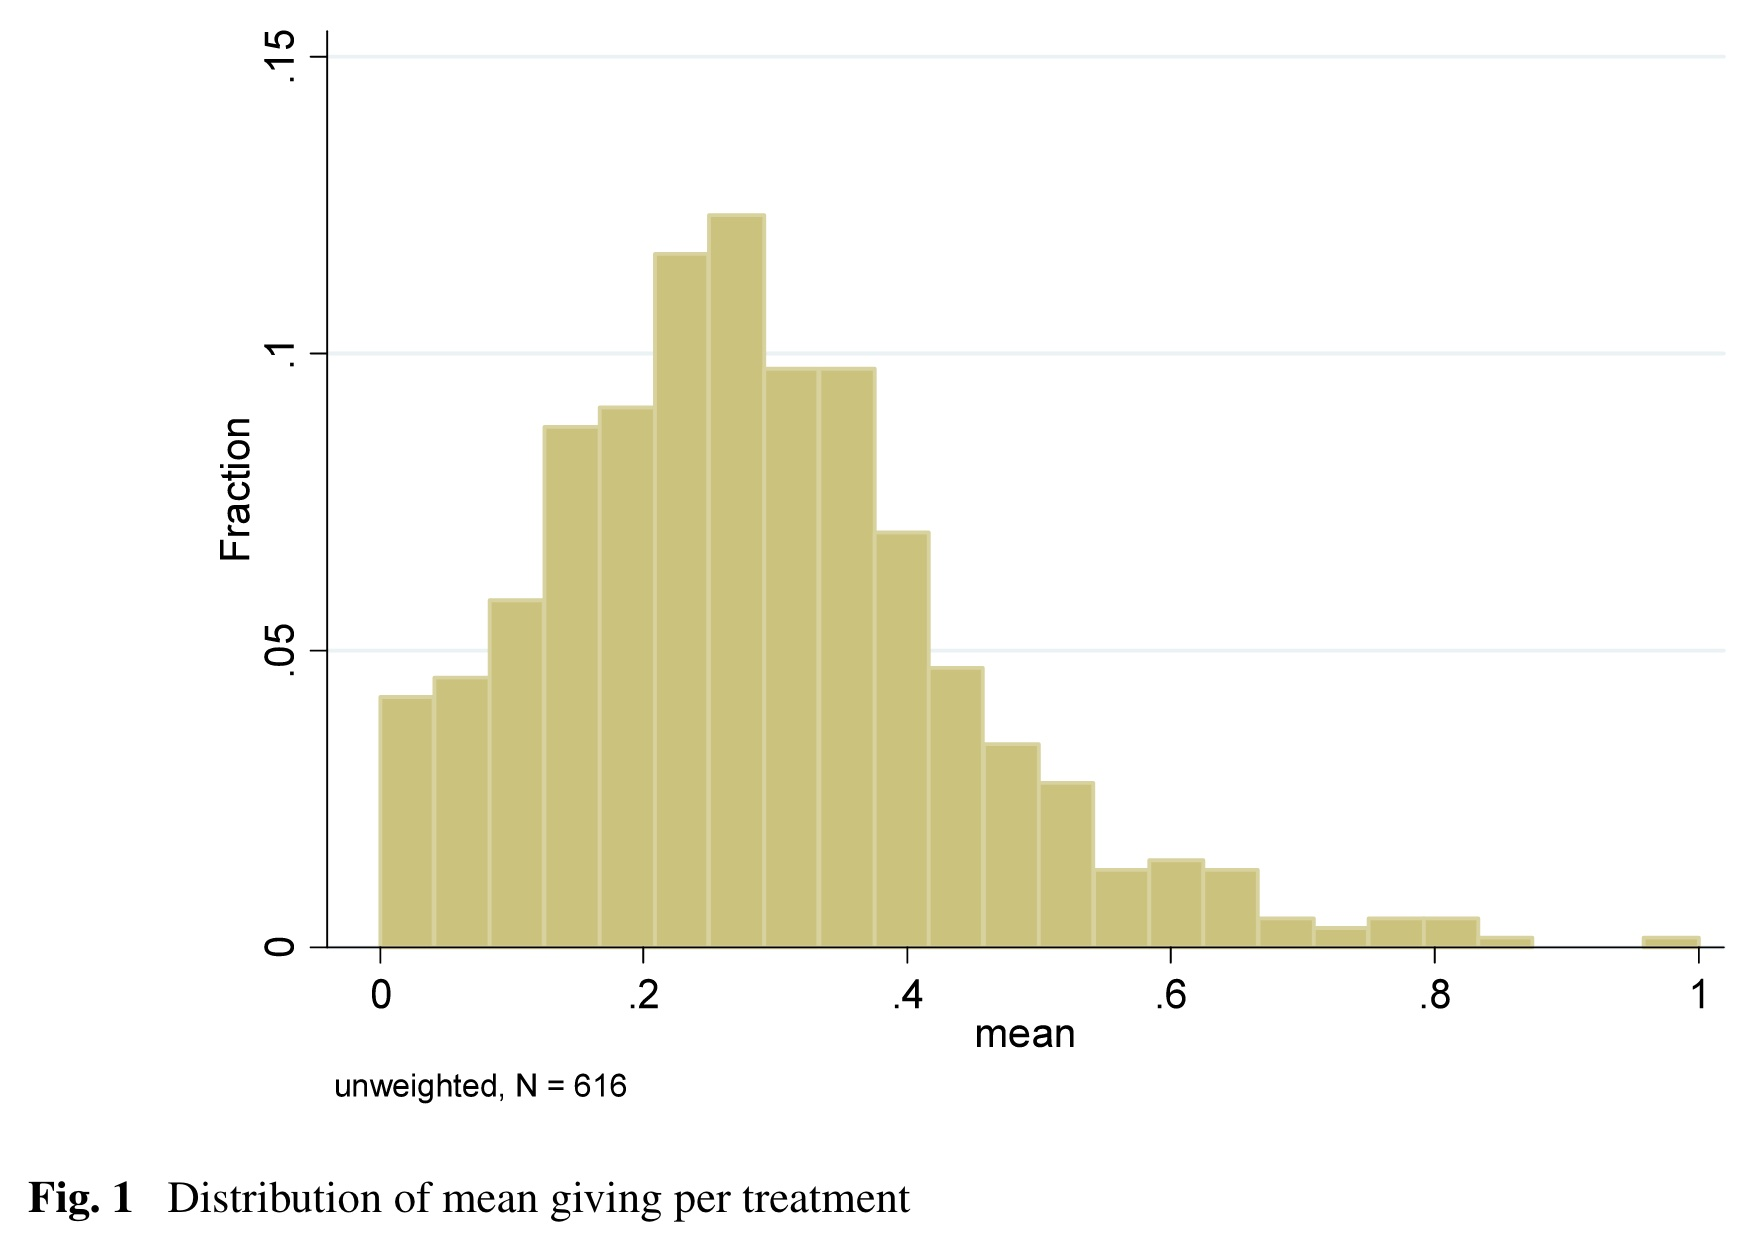
\includegraphics{social-preferences/img/engel-2011-fig-1.jpg}

}

}

\subcaption{\label{fig-engel2}Individual give rates}
\end{minipage}%

\caption{\label{fig-dictator}Distribution of amount given in the
dictator game (Engel, 2011).}

\end{figure}

\hypertarget{social-preferences-1}{%
\section*{Social preferences}\label{social-preferences-1}}
\addcontentsline{toc}{section}{Social preferences}

\markright{Social preferences}

The results of these two games are evidence of social preferences, or
what are sometimes called ``other-regarding preferences''.

People do not care solely about their own outcomes.

In this subject we will examine the following types of social
preferences.

\begin{itemize}
\item
  Distribution: People care about the split of the resources. Reasons
  for distributional preferences include:

  \begin{itemize}
  \item
    Altruism: People care about others.
  \item
    Inequality aversion: People care about the relative distribution.
  \end{itemize}
\item
  Reputation: People care about what other people think. They fear the
  social stigma that can result from ``selfish'' behaviour.
\item
  Reciprocity: We care about the intentions of others and often
  reciprocate others' actions.
\end{itemize}

\hypertarget{distribution}{%
\chapter{Distribution}\label{distribution}}

Distributional preferences are preferences that relate to the amount of
money or resources each person gets or has.

It is often easy to incorporate distributional preferences into economic
analysis as they are a natural extension of how economists think about
individuals' preferences. We can extend the typical assumption that a
person only cares about their own material outcomes to other people.

\hypertarget{altruism}{%
\section{Altruism}\label{altruism}}

Altruism is concern for the outcomes of others.

To incorporate altruism, we simply need to provide a positive weight to
the utility of others in the utility function \(U_i(x_i,x_j)\), where
\(U_i\) is the utility of agent \(i\), \(x_i\) the outcome for agent
\(i\) and \(x_i\) the outcome for agent \(j\).

An example utility function might be:

\[
U_i(x_i,x_j)=x_i+\alpha x_j
\]

where \(\alpha>0\).

Altruism might have different drivers:

\begin{itemize}
\item
  Pure altruism: genuine concern for others' wellbeing.
\item
  Impure altruism: A ``warm glow'' where people feel good about doing
  good without actually caring about the others' wellbeing.
\end{itemize}

Altruism, however, is insufficient to explain the experimental results,
such as those in the ultimatum game. While it could predict non-zero
offers by the proposer, it does not predict rejection of any offers by
the responder. Rejection harms both the responder and the proposer.

The proposer could only reject if a negative weight was applied to
either their own or the proposer's outcome.

\hypertarget{inequality-aversion}{%
\section{Inequality aversion}\label{inequality-aversion}}

The idea behind inequality aversion is that people may have:

\begin{itemize}
\item
  A dislike of having less than other people
\item
  A dislike of having more than other people.
\end{itemize}

\hypertarget{the-fehr-schmidt-model}{%
\subsection{The Fehr-Schmidt model}\label{the-fehr-schmidt-model}}

Consider the following version of the utility function in Fehr and
Schmidt (1999):

\[
U_i(x_i,x_j)=x_i-\alpha\text{max}\{x_j-x_i,0\}-\beta\text{max}\{x_i-x_j,0\}
\]

The three terms in this function represent:

\begin{itemize}
\item
  The utility of their own outcome \(x_i\)
\item
  Their dislike of having less than the other agent (with \(\alpha>0\))
\item
  Their dislike of having more than the other agent (where \(\beta>0\))
\end{itemize}

Typically \(\alpha>\beta\) as people dislike having less than others
than they dislike having more than others. We could also set \(\beta<0\)
for an agent that likes to be better off than others.

This utility function has a kink at \(x_j\) where the agent \(i\) moves
from having less to more than agent \(j\). If \(0<\beta<1\) as in this
diagram, \(U(x_i)\) continues to increase in \(x_i\) above \(x_j\), but
at a decreasing rate as inequality degrades the benefits of having more.

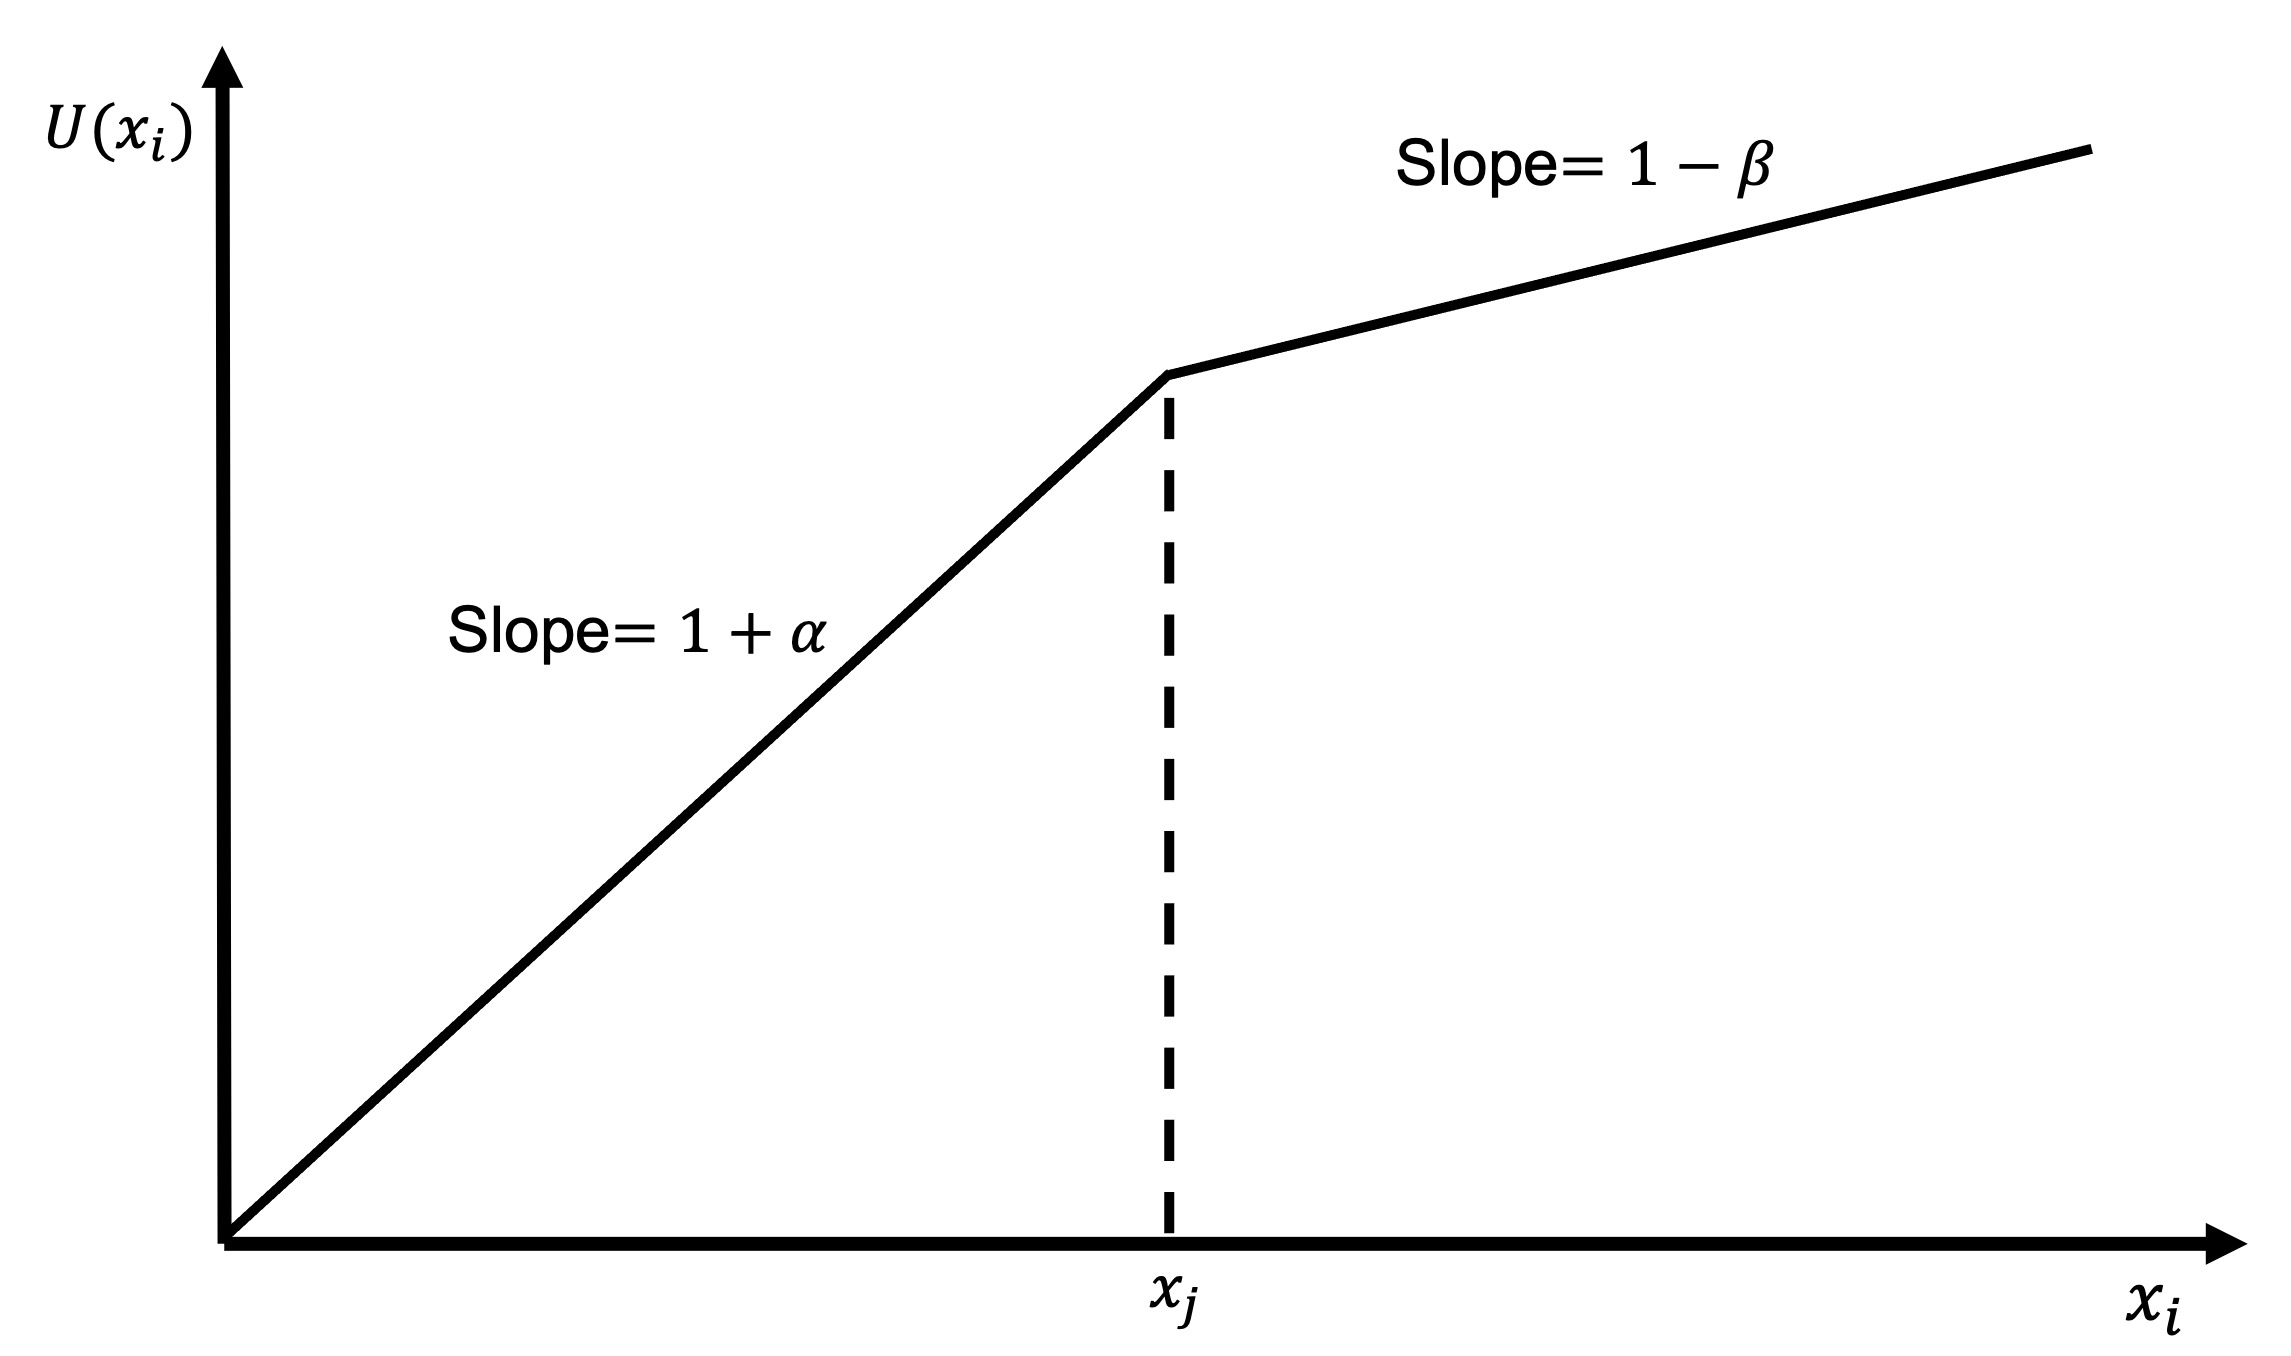
\includegraphics{social-preferences/img/inequality-aversion-1.jpg}

\hypertarget{the-ultimatum-game-2}{%
\subsection{The ultimatum game}\label{the-ultimatum-game-2}}

Suppose two players of the ultimatum game have preferences of this form.

What offers \(x\) would the responder reject where the proposer has \$10
to split between them?

If the responder rejects, \(x_P=x_R=0\).

If the responder accepts, \(x_P=10−x\) and \(x_R=x\).

The responder will accept if:

\begin{align*}
U_R(\text{accept})&>U_R(\text{reject}) \\[6pt]
x_R−\alpha\text{max}\{x_P−x_R,0\}−\beta\text{max}\{x_R−x_P,0\}&>0 \\[6pt]
x−\alpha\text{max}\{10−x−x,0\}−\beta\text{max}\{x−(10−x),0\}&>0 \\[6pt]
x−\alpha\text{max}\{10−2x,0\}−\beta\text{max}\{2x−10, 0\}&>0 \\
\end{align*}

If the offer is more than \$5:

\begin{align*}
x−\beta\text{max}\{2𝑥−10, 0\}>0 \\[6pt]
x−\beta(2x−10)>0 \\[6pt]
(1−\beta)x+\beta(10−x)>0
\end{align*}

This will always hold for any \(\beta<1\), so the responder will always
accept offers greater than \$5.

If the offer is less than \$5:

\begin{align*}
x−\alpha\text{max}\{10−2x,0\}>0 \\
x−\alpha(10−2x)>0 \\
(1+\alpha)x−\alpha(10−𝑥)>0
\end{align*}

Whether this holds depends on the value of \(\alpha\) and the precise
size of \(x\). If \(\alpha=1/2\), then:

\begin{align*}
(1+1/2)x−1/2 (10−x)&>0 \\
2x−5&>0 \\
x&>2.5
\end{align*}

A responder with \(\alpha=1/2\) will reject any offer under \$2.50.

We can plot the utility function for this game as the size of the offer
increases. As the offer is not independent of the proposer's payoff, we
will first derive the shape of the utility curve as a function of
\(x_R\).

\begin{align*}
U_R(x_P,x_R)&=x_R-\alpha\text{max}\{x_P-x_R,0\}-\beta\text{max}\{x_R-x_P,0\} \\
&=x-\alpha\text{max}\{10-2x,0\}-\beta\text{max}\{2x-10,0\}
\end{align*}

\[
U_R(x_P,x_R)=\left\{\begin{matrix}
(1+2\alpha)x−10\alpha \quad &\textrm{if} \quad x \geq 0 \\[6pt]
(1−2\beta)x+10\beta \quad &\textrm{if} \quad x < 0 
\end{matrix}\right.
\]

The slope of each of these curves is twice that we saw earlier as any
increase in outcome for the responder is matched by a decrease in
outcome for the proposer (and vice versa).

This diagram shows the responder's utility curve as a function of the
offer \(x\).

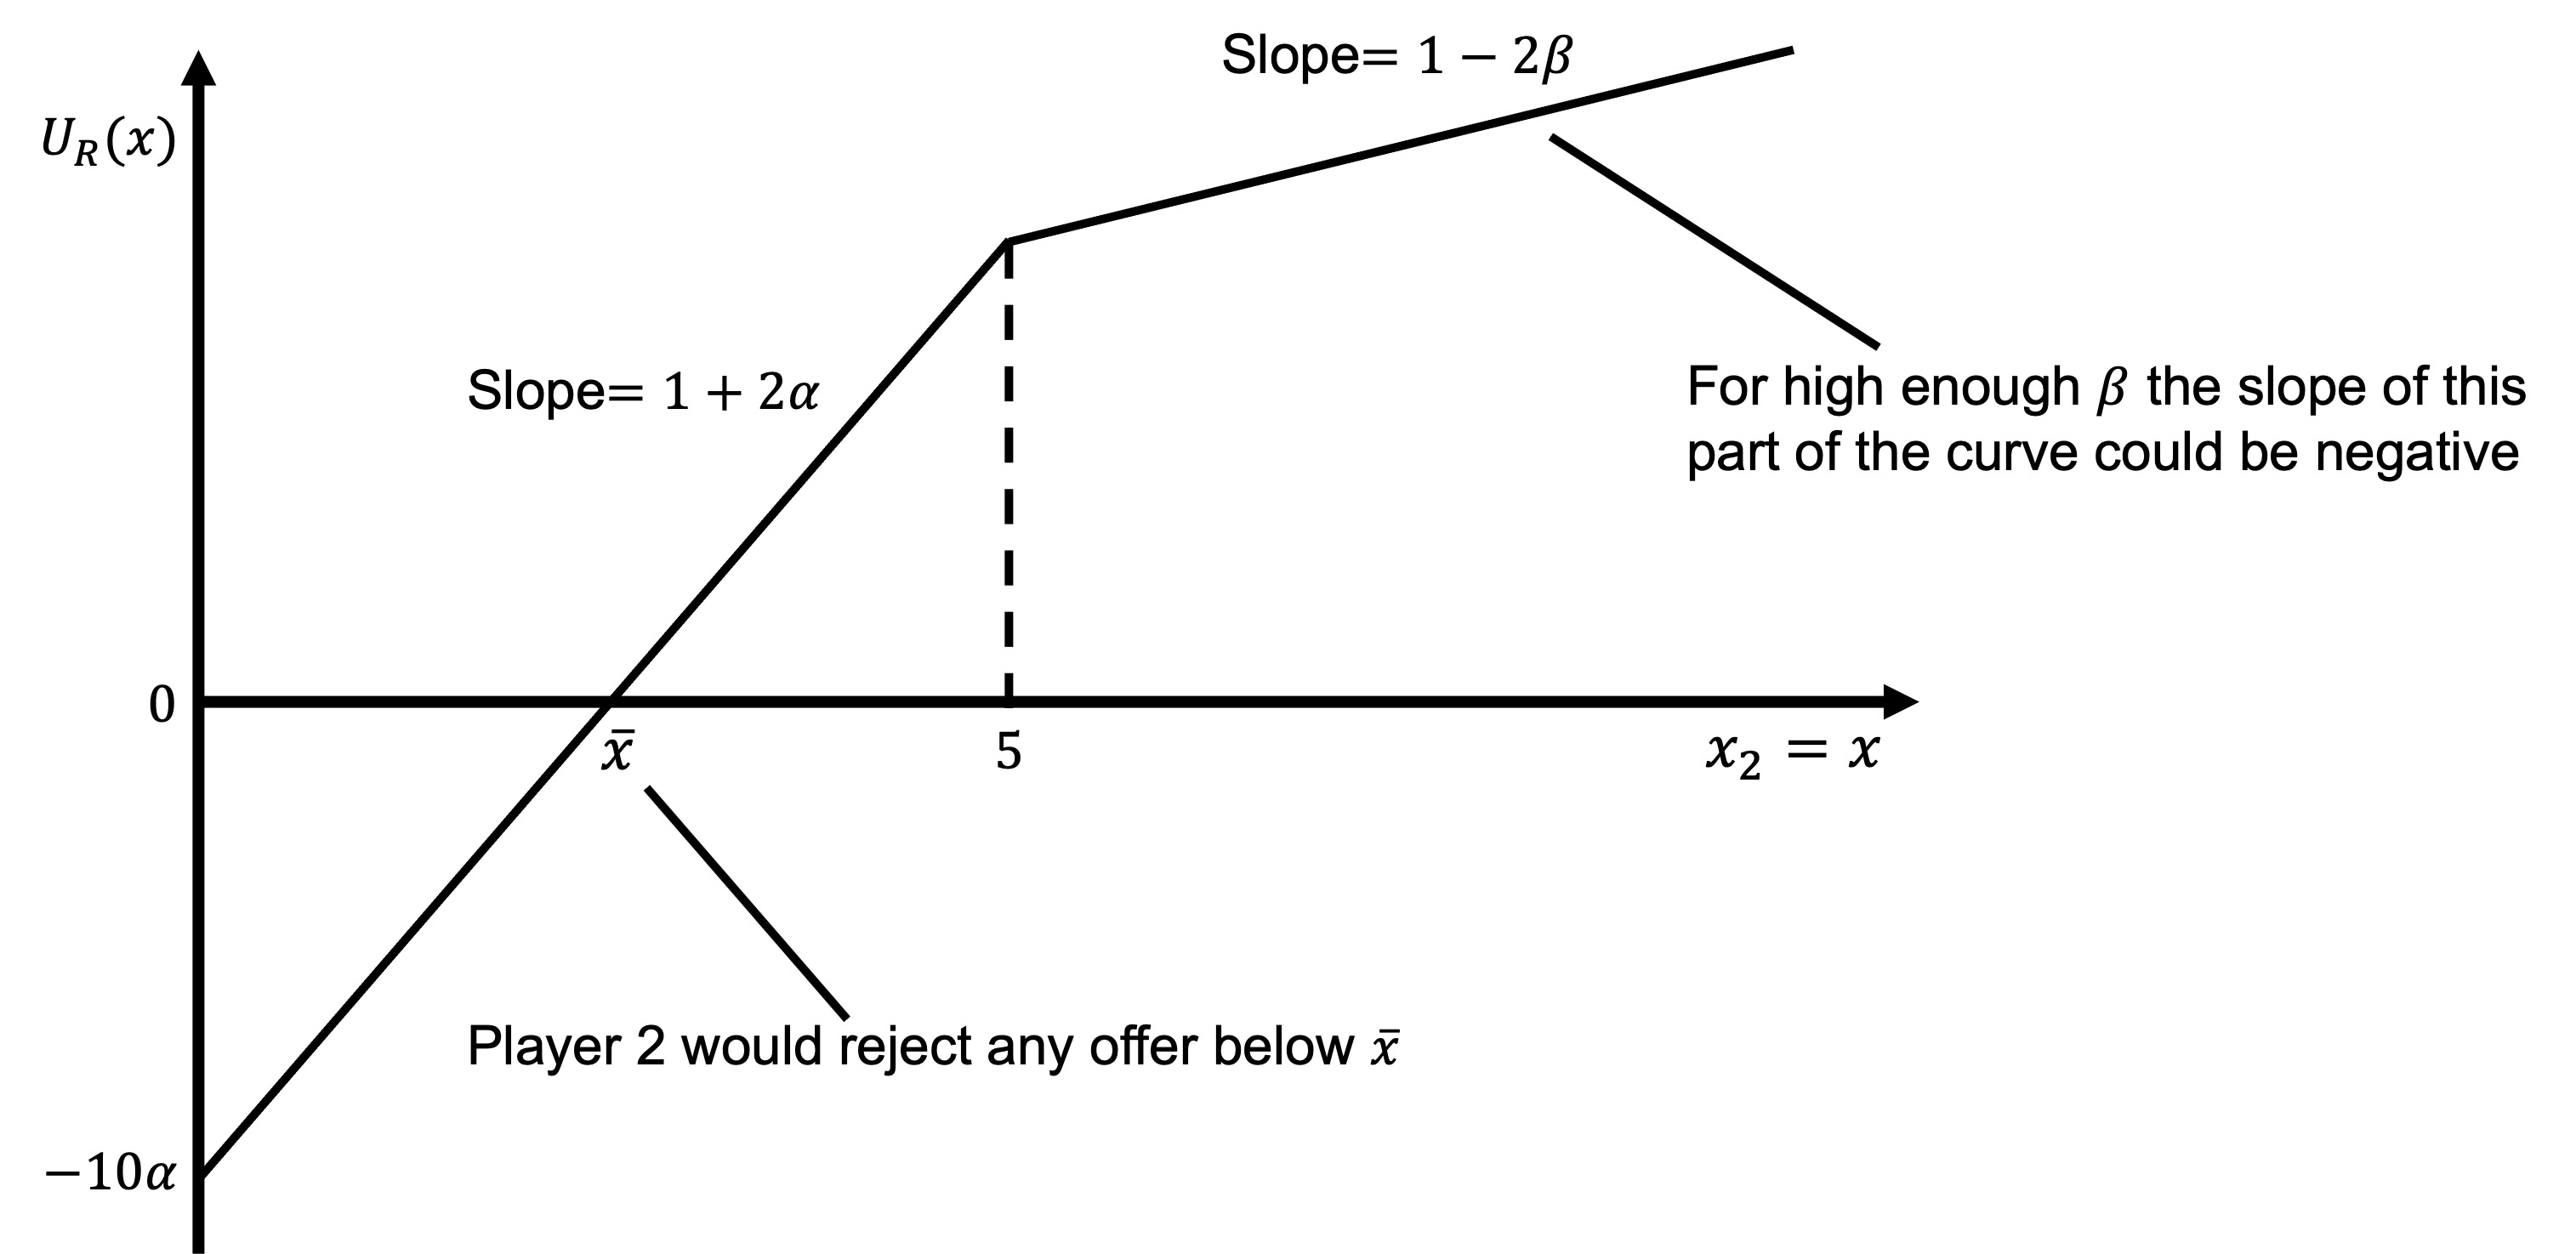
\includegraphics{social-preferences/img/inequality-aversion-2.jpg}

\hypertarget{a-general-model-of-distributional-preferences}{%
\section{A general model of distributional
preferences}\label{a-general-model-of-distributional-preferences}}

Charness and Rabin (2002) offer a more general utility function that
captures the possible forms of distributional preference:

\[
u_i(x_i,x_j)=\left\{\begin{matrix}
\rho x_j+(1-\rho)x_i \quad &\textrm{if} \quad x_i \geq x_j \\[6pt]
\sigma x_j+(1-\sigma)x_i \quad &\textrm{if} \quad x_i < x_j 
\end{matrix}\right.
\]

An agent's attitudes toward others depends on their relative position:
When the agent is ahead of other, the other player's welfare enters
their utility via \(\rho\) When the agent is behind the other, the other
player's welfare enters dictator's utility via σ For most of people
\(\rho>\sigma\). They are more willing to give weight to others' utility
when they are better off. It can also be that \(\sigma<0\). If they are
behind the other they place negative weight on further gains by that
other.

Consider the following example.

Suppose a dictator has \(\sigma=−1/2\) (they have less than the other
player, so \(\sigma\) is the relevant parameter) and must decide between
the two discrete allocations (1, 0) and (5, 1):

\begin{align*}
U(1,0)&=\sigma\times 1+(1−\sigma)\times 0 \\
&=−1/2×1+(1+1/2)\times 0 \\
&=−1/2 \\[6pt]
U(5,1)&=\sigma\times 5+(1−\sigma)\times 1 \\
&=−1/2×5+(1+1/2)\times 1 \\
&=−1
\end{align*}

\(\sigma<0\) can also account for the rejection of low offers in the
ultimatum game.

This model can capture distributional preferences as follows.

\(1≥\rho≥\sigma≥0\): altruism

\(1≥\rho≥0≥\sigma\): inequality aversion

\(0≥\rho≥\sigma\): status-seeking

\(\rho=\sigma=0\): the classical self-interested utility function

\(\rho=1\), \(\sigma=0\): \(u_i(x_i,x_j)=\text{min}\{x_i,x_j\}\), which
equates to Rawlsian preferences whereby the agent seeks greatest benefit
for the least advantaged

\(\rho=\sigma=1/2\): \(u_i(x_i,x_j)=x_i+x_j\), which equates to
utilitarian preferences whereby the agent seeks to maximise total
utility

\hypertarget{example-the-trust-game}{%
\subsection{Example: the trust game}\label{example-the-trust-game}}

In Tutorial 9 we considered whether Linda should invest in Marco's
startup:

\begin{quote}
Linda is looking for investment opportunities. She identifies a
promising crypto-based start-up created by an Marco. Marco is looking
for seed funding.

Linda can invest \$10.

If Linda invests, her investment will triple in value. Marco can then
decide to either shut down the start-up and keep the \$30 or maintain
the start-up in the market and pay a \$15 dividend to each of Linda and
himself.

If Linda does not invest, Linda keeps the \$10. The start-up gets \$0.
\end{quote}

We determined that Linda would not invest.

Suppose now that Linda and Marco have preferences as follows:

\[
U_L(x_L,x_M)=\left\{\begin{matrix}
\frac{1}{3}x_L+\frac{2}{3}x_M \quad &\textrm{if} \quad x_L \geq x_M\\[6pt]
\frac{2}{3}x_L+\frac{1}{3}x_M \quad &\textrm{if} \quad x_L < x_M 
\end{matrix}\right. \\
\\[12pt]
U_M(x_L,x_M)=\left\{\begin{matrix}
\frac{3}{4}x_L+\frac{1}{4   }x_M \quad &\textrm{if} \quad x_M \geq x_L\\[6pt]
x_M \quad &\textrm{if} \quad x_M < x_L 
\end{matrix}\right.
\]

Where \(x_L\) and \(x_M\) are the outcomes for Linda and Marco
respectively.

Marco and Linda know each others utility functions.

What is the equilibrium with these distributional preferences? Explain
the intuition.

If Linda chooses trust, Marco has a choice between \$15 each and \$30
for himself.

\[
U_M(x_L,x_M)=\left\{\begin{matrix}
\frac{3}{4}x_L+\frac{1}{4}x_M \quad &\textrm{if} \quad x_M \geq x_L\\[6pt]
x_M \quad &\textrm{if} \quad x_M < x_L 
\end{matrix}\right. \\
\\[12pt]
U_M(15,15)=\frac{3}{4}(15)+\frac{1}{4}(15)=15 \\
\\[12pt]
U_M(0,30)=\frac{3}{4}(0)+\frac{1}{4}(30)=7.5
\]

Marco receives higher utility by paying the dividend to Linda.

Linda also has utility from each distribution.

\[
U_L(x_L,x_M)=\left\{\begin{matrix}
\frac{1}{3}x_L+\frac{2}{3}x_M \quad &\textrm{if} \quad x_L \geq x_M\\[6pt]
\frac{2}{3}x_L+\frac{1}{3}x_M \quad &\textrm{if} \quad x_L < x_M 
\end{matrix}\right. \\
\\[12pt]
U_L(15,15)=\frac{1}{3}(15)+\frac{2}{3}(15)=15 \\
\\[12pt]
U_L(0,30)=\frac{2}{3}(0)+\frac{1}{3}(30)=10
\]

For the other node, if Linda does not invest, she will keep \$10. Marco
will have nothing.

\begin{align*}
U_M(10,0)=0 \\
\\
U_L(10,0)=\frac{1}{3}(10)+\frac{2}{3}(0)=3.33
\end{align*}

Putting those payoffs into the extensive form of the game, we get the
following:

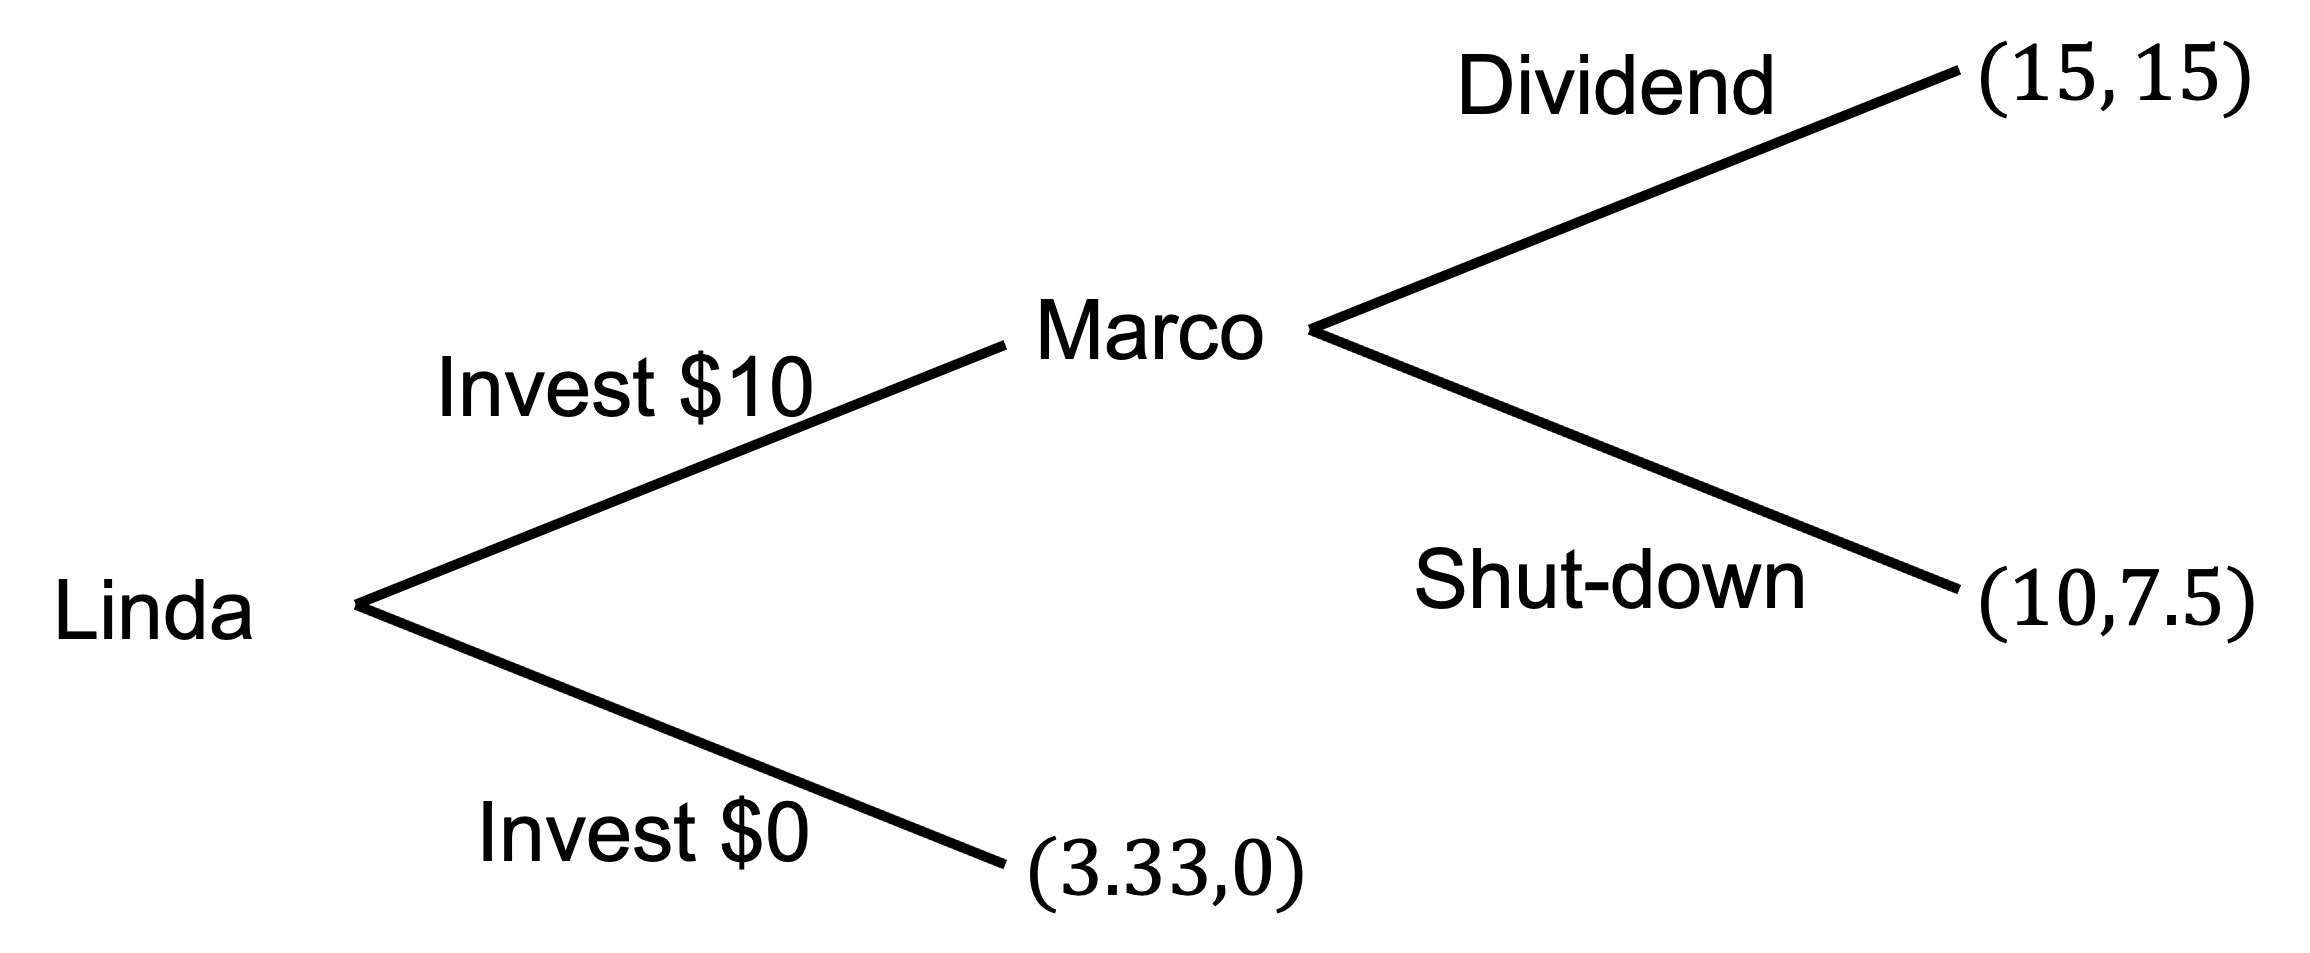
\includegraphics{social-preferences/img/trust-distributional-1.jpg}

The new equilibrium is that Macro will return a dividend, so Linda
invests.

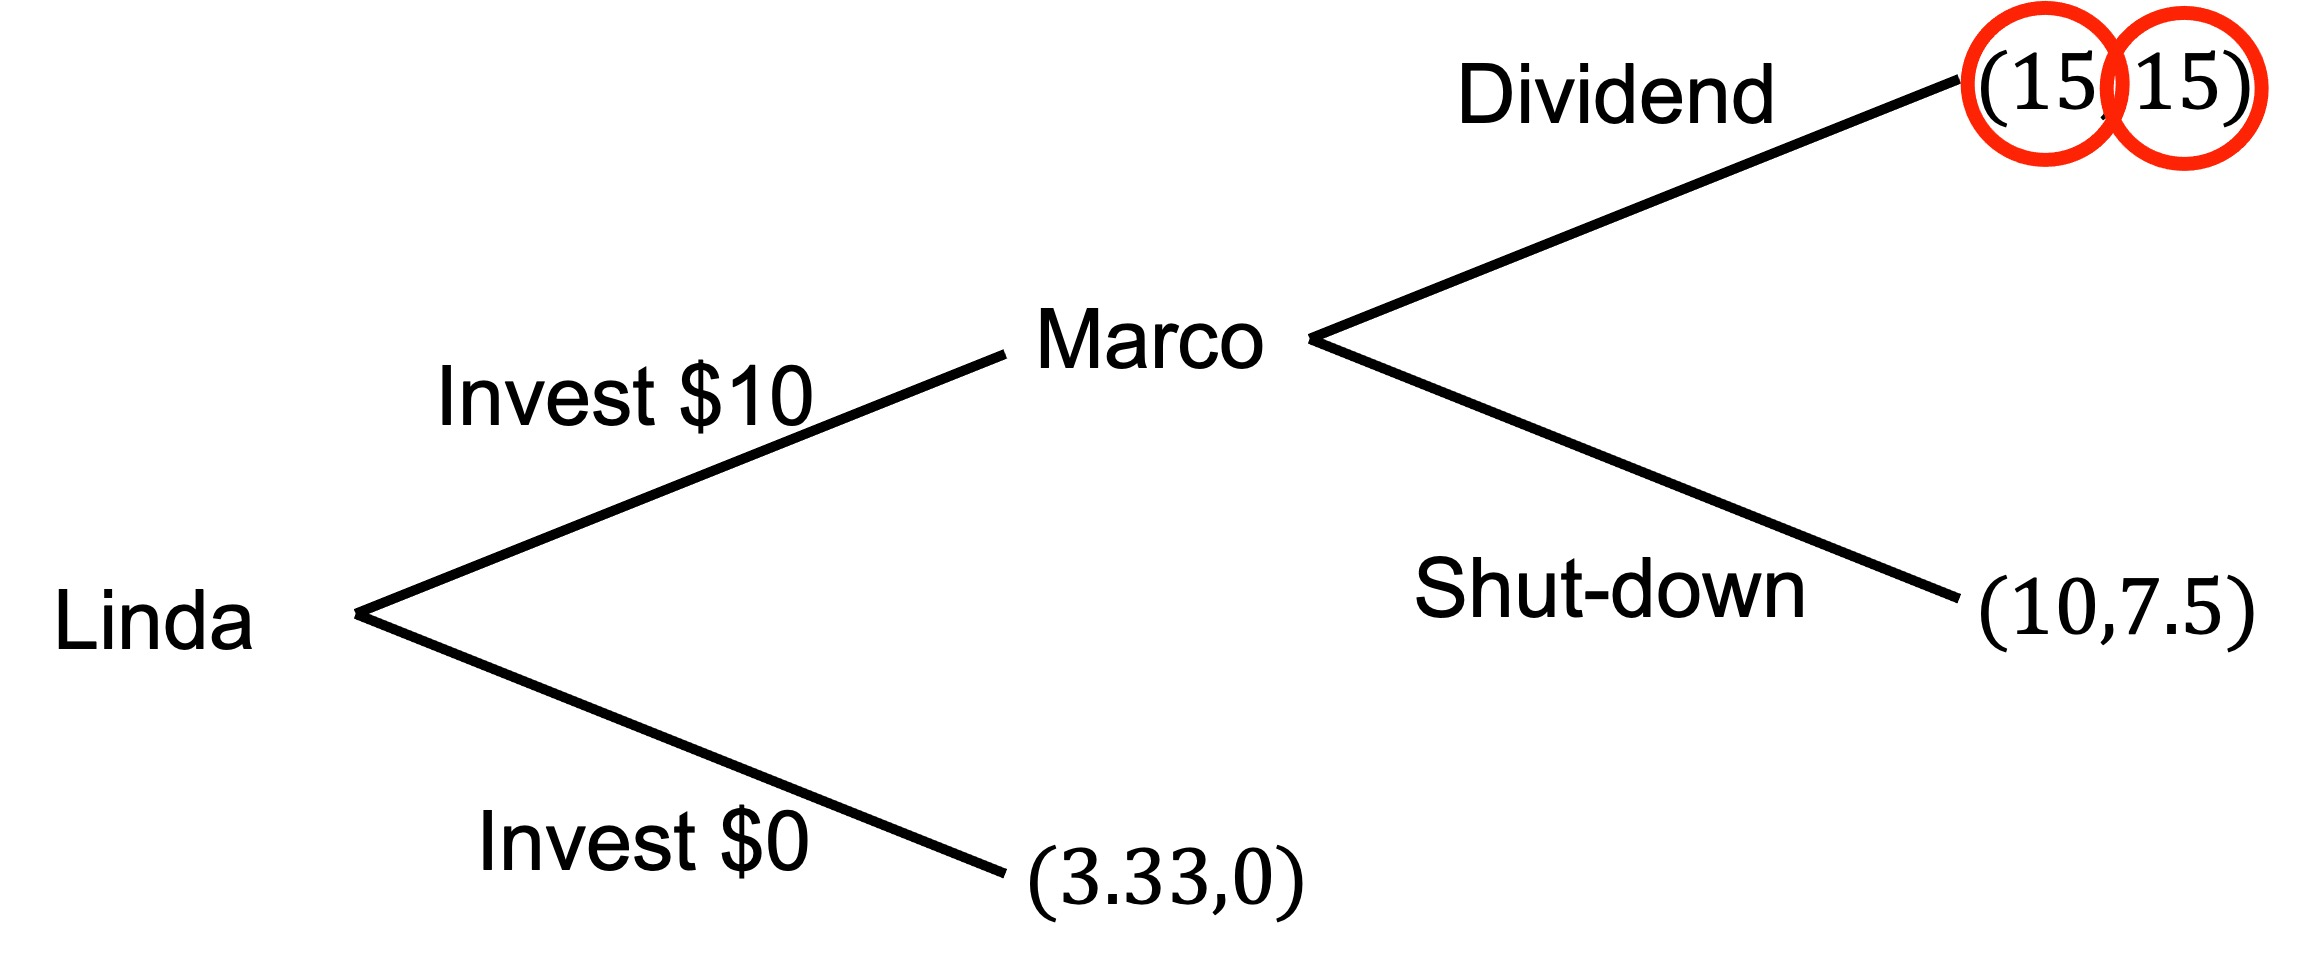
\includegraphics{social-preferences/img/trust-distributional-2.jpg}

\hypertarget{reputation}{%
\chapter{Reputation}\label{reputation}}

People care about what other people think. They fear the social stigma
that can result from ``selfish'' behaviour.

Partly this is for strategic reasons. For example, to attract reciprocal
behaviour, people may need to be aware of your intentions.

However, there is also evidence that people simply care about what other
people think.

\hypertarget{saving-face}{%
\section{Saving face}\label{saving-face}}

Andreoni and Bernheim (2009) ran a non-anonymous dictator game.

Each dictator was endowed with \$20.

A computer then chose a distribution between the dictator and the
receiver, selecting either (\$0, \$20) or (\$20, \$0) with equal
probability. The dictator observes the allocation chosen by the
computer, but the receiver does not.

The computer's allocation is then implemented with a probability \(p\).
This probability is known to both the dictator and receiver.

If the dictators choice is to be implemented, the dictator makes a split
of the \$20. The receiver learns only the allocation. They do not learn
the dictator's choice.

Distributional preferences predict that \(p\) should not affect the
dictator's choice. The dictator should just think about the situation in
which their choice matters.

However, the experimental results did not conform with this prediction.
Dictators condition their decision on the common knowledge of \(p\).

This chart shows how offers change with \(p\) where the computer will
offer 0 if selected.

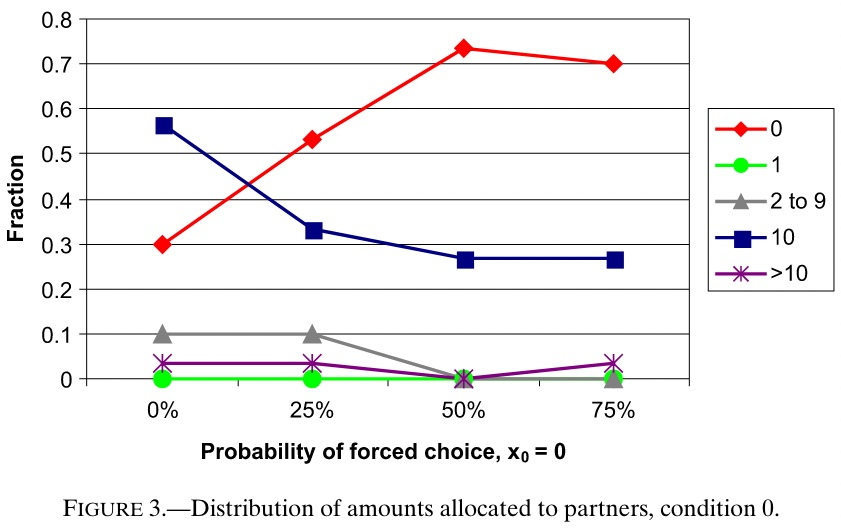
\includegraphics{social-preferences/img/andreoni-and-bernheim-2009-fig-3.jpg}

For high \(p\) and a computer allocation of 0 to the receiver, most
dictators will offer 0.

For \(p\) close to 0 and a computer allocation of 0 to the receiver, the
majority of dictators will offer \$10 to the receiver.

For low \(p\), if the receiver receives a low allocation, they will
likely infer it is due to the dictator's decision. The dictator appears
to care about their reputation in the eyes of the receiver.

\hypertarget{reciprocity}{%
\chapter{Reciprocity}\label{reciprocity}}

Reciprocity is the response of like for like behaviour. Kindness is
responded to with kindness. Unkindness is responded to with unkindness.

Reciprocity might be considered to have two forms:

\begin{itemize}
\item
  Instrumental reciprocity: Agents reciprocate behaviour due to the
  long-term benefits of sustained cooperation. The behaviour is
  motivated by the positive trade-off between long-term and short-term
  gains.
\item
  Intrinsic reciprocity: Agents reciprocate behaviour despite the
  absence of long-term gains.
\end{itemize}

\hypertarget{intentions}{%
\section{Intentions}\label{intentions}}

Consider this variation of the ultimatum game.

Scenario 1:

\begin{itemize}
\item
  A proposer has a choice between offering a split of (\$8, \$2) or
  (\$5, \$5).
\item
  Responders tend to reject offers of (\$8, \$2).
\end{itemize}

Scenario 2:

\begin{itemize}
\item
  A proposer has a choice between offering a split of (\$8, 2) or (\$10,
  0).
\item
  Responders tend to accept offers of (\$8, \$2).
\end{itemize}

How can (\$8, \$2) be better than (\$0, \$0) in one scenario but not in
the other?

We often reject ``unfair'' offers.

Rejection in this case cannot be explained by distributional concerns.
Rejection is sensitive to disclosure about the remaining part of the
decision tree.

Responders do not base their decision on the final outcome alone. They
consider the proposer's intentions and reciprocate them.

A proposer who offers \$2 instead of \$0 is seen as having good
intentions. A proposer who offers \$2 instead of \$5 is seen as having
bad intentions.

\hypertarget{the-trust-game-1}{%
\section{The trust game}\label{the-trust-game-1}}

Recall the trust game.

\begin{quote}
The trust game involves two players: a sender and a receiver

Both the sender and receiver are given an initial sum \(m\).

The sender sends a share \(x\) of their \(m\) to the receiver (the
investment).

Before the investment is received by the receiver, it is multiplied by
some factor \(k\).

The receiver receives \(kx\).

The receiver then returns to the sender some share \(y\) of their total
allocation \(m+kx\).

The final outcome is: (\(m−x+y\), \(m+kx−y\))
\end{quote}

We identified that the game theoretic equilibrium was for the receiver
to return nothing, so the sender sends nothing.

What happens in experimental settings?

\begin{itemize}
\item
  Senders tend to send a positive amount, typically around half of their
  endowment.
\item
  Receivers tend to send back a bit less than is sent.
\end{itemize}

\begin{figure}

\begin{minipage}[t]{0.50\linewidth}

{\centering 

\raisebox{-\height}{

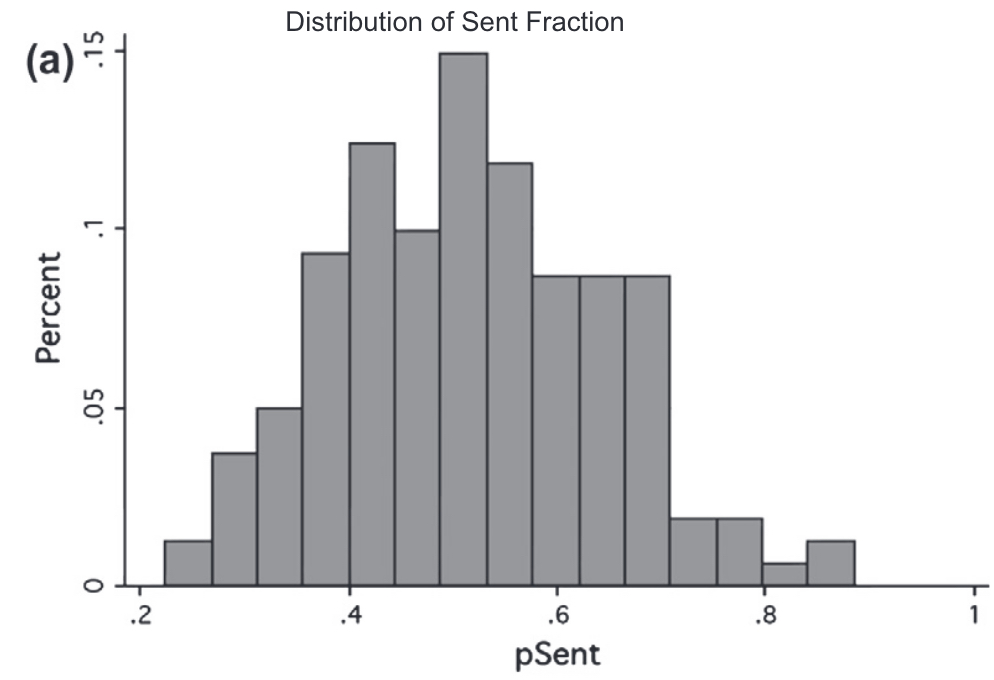
\includegraphics{social-preferences/img/johnson-and-mislin-2011-fig-1a.jpg}

}

}

\subcaption{\label{fig-johnson1a}Sent}
\end{minipage}%
%
\begin{minipage}[t]{0.50\linewidth}

{\centering 

\raisebox{-\height}{

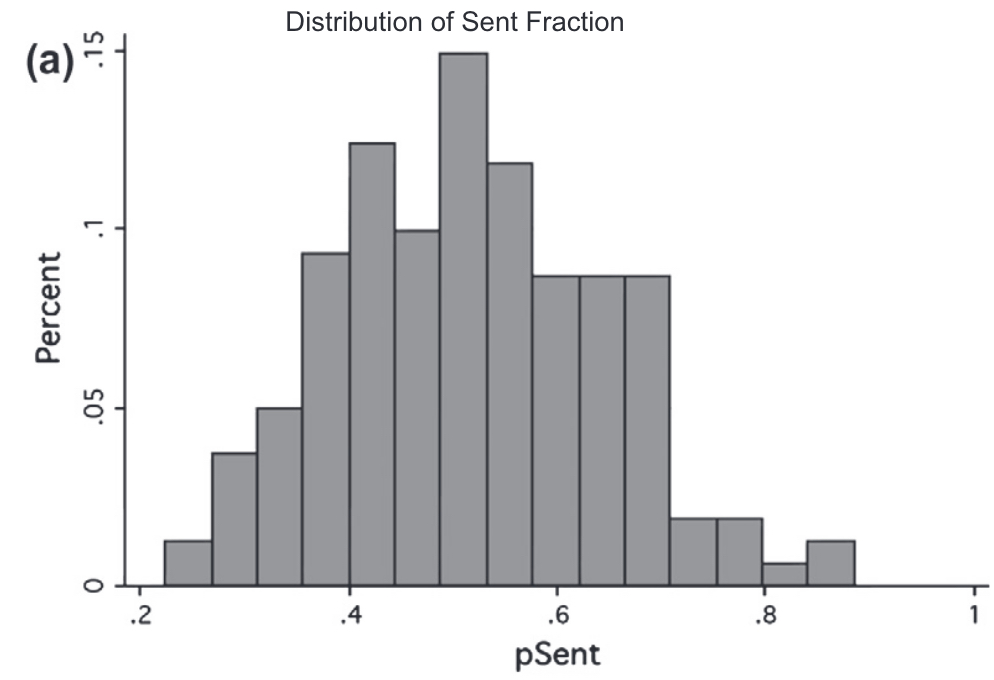
\includegraphics{social-preferences/img/johnson-and-mislin-2011-fig-1a.jpg}

}

}

\subcaption{\label{fig-johnson1b}Returned}
\end{minipage}%

\caption{\label{fig-trust}Distribution of proportion sent and proportion
returned in 162 replications of the trust game (N. D. Johnson and
Mislin, 2011).}

\end{figure}

Why do players do this? Possible explanations are:

\begin{itemize}
\item
  The receiver feels that they must reciprocate the sender's investment
  (they are responding to their intentions). The amount returned might
  be considered a measure of ``trustworthiness''.
\item
  The sender trusts that due to these factors some of their investment
  will be repaid.
\end{itemize}

The receiver's behaviour is also consistent with altruism and inequality
aversion.

\hypertarget{the-public-goods-game-1}{%
\section{The public goods game}\label{the-public-goods-game-1}}

Recall the public goods game.

\begin{quote}
N participants are given an initial endowment.

Each secretly and simultaneously chooses how much of their endowment
they wish to contribute to a public pot.

The money in the public pot is multiplied by some amount \(m\) and split
evenly between the players.

For example, players might each be given \$10, with the pot doubled.
\end{quote}

In Nash equilibrium in the public goods game, nobody transfers anything
to the pot. Any contributions are split between all players, so if there
are more players than \(m\) (which is normally the case by design),
contributions result in a loss.

What do people do when playing the public goods game in the lab?

In a meta-analysis, Zelmer (2003) found an average contribution of 38\%
of the endowment. This was larger the higher the marginal per capita
return (i.e.~the higher \(m/N\))

One possible explanation is that players trust that the other players
will contribute, so they desire to reciprocate the expected
contributions from others.

Another explanation hinges on social norms. Where a norm of behaviour
exists, people tend to follow it.

\hypertarget{social-preferences-examples}{%
\chapter{Social preferences
examples}\label{social-preferences-examples}}

\hypertarget{advice}{%
\section{Advice}\label{advice}}

Agent A is going to their financial adviser to buy some life insurance.
The adviser can sell them insurance that does not cover heart attacks
but for which the adviser receives a huge sales commission (bad
insurance). Or the adviser can sell Agent A comprehensive insurance for
which their sales commission is lower (good insurance).

The payoffs \((x,y)\) for each decision are indicated in the game tree
below, with \(x\) being the satisfaction of Agent A and \(y\) being the
satisfaction of the adviser.

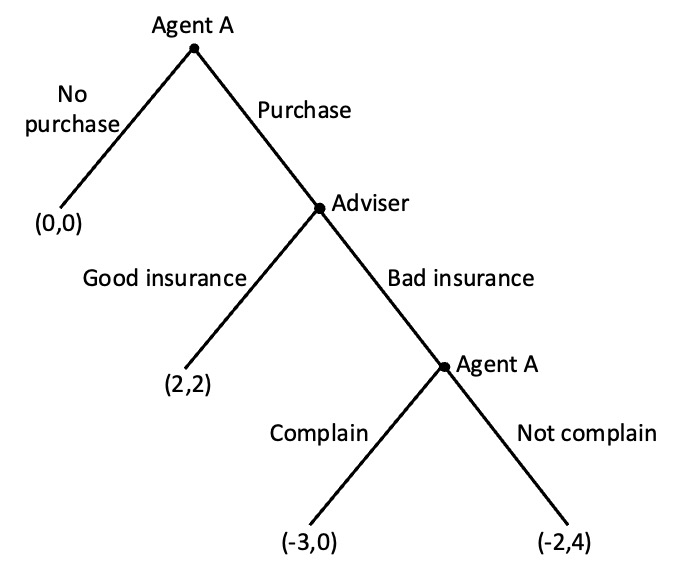
\includegraphics[width=0.6\textwidth,height=\textheight]{social-preferences/img/adviser-1.jpg}

\begin{enumerate}
\def\labelenumi{\alph{enumi})}
\tightlist
\item
  Assume the adviser only cares about the payoffs indicated. What would
  the adviser do if Agent A chooses to purchase?
\end{enumerate}

The adviser will compare payoffs of 4 for selling bad insurance and 2
for selling good insurance. They will choose to sell bad insurance.

\begin{enumerate}
\def\labelenumi{\alph{enumi})}
\setcounter{enumi}{1}
\tightlist
\item
  What would Agent A do, anticipating the choice of the adviser?
\end{enumerate}

Agent A will compare a payoff of 0 for no purchase and a payoff of -2
for purchase (knowing that they will be sold bad insurance). They will
choose not to buy insurance.

\begin{enumerate}
\def\labelenumi{\alph{enumi})}
\setcounter{enumi}{2}
\tightlist
\item
  Suppose the adviser has social preferences, with a distaste for
  inequality. If the payoffs \(x\) for Agent A and \(y\) for the adviser
  are unequal, the adviser experiences a dissatisfaction and their
  payoff becomes \(y-3\). What would happen to the outcome in this case?
\end{enumerate}

The adviser's payoff for selling the bad insurance is now \(4-3=1\).
This is less than the payoff of 2 they receive for selling good
insurance. They will now sell good insurance.

Agent A now has a choice of a payoff of 0 for not purchasing insurance,
and 2 for purchasing. They make the purchase.

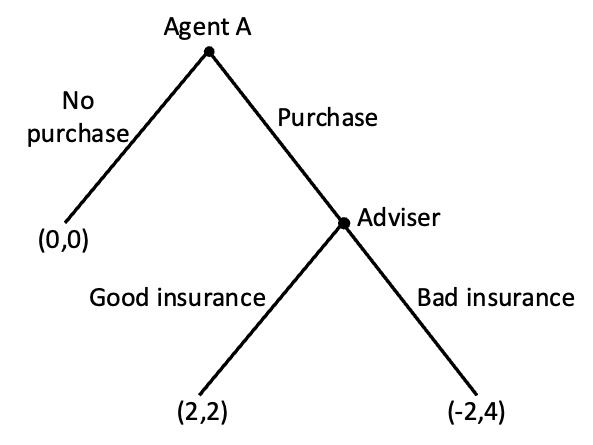
\includegraphics[width=0.6\textwidth,height=\textheight]{social-preferences/img/adviser-2.jpg}

\begin{enumerate}
\def\labelenumi{\alph{enumi})}
\setcounter{enumi}{3}
\tightlist
\item
  Suppose now that Agent A can complain to the regulator if they are
  sold bad insurance. If Agent A is successful, they can cancel the
  insurance but would suffer a cost of -3 due to the effort involved.
  Would this change the outcome of the game?
\end{enumerate}

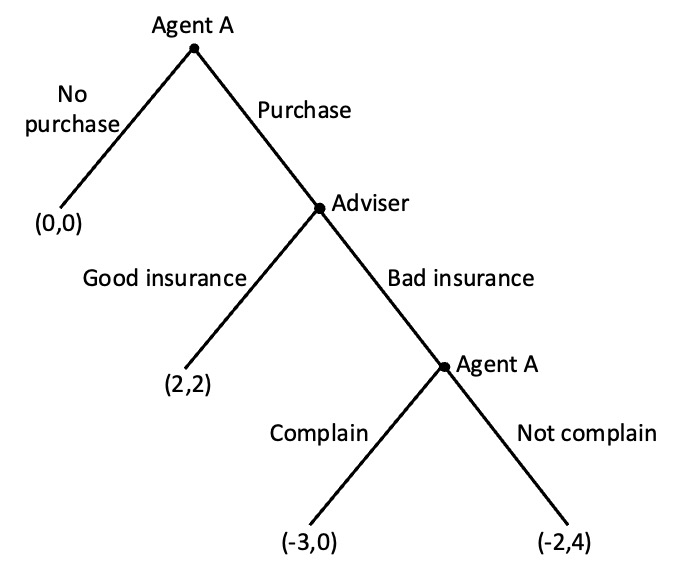
\includegraphics[width=0.6\textwidth,height=\textheight]{social-preferences/img/adviser-3.jpg}

Working by backward induction: Agent A has a choice between complaining
for a payoff of -3 or not complaining for a payoff of -2. They do not
complain.

The rest of the game plays out as per questions a) and b). There is no
change to the outcome as they cannot commit to complain in advance (at
least in this version of the game). The threat to complain is not
credible.

\begin{enumerate}
\def\labelenumi{\alph{enumi})}
\setcounter{enumi}{4}
\tightlist
\item
  Suppose Agent A has a reputation for seeking revenge and would
  experience satisfaction of +4 from complaining to the regulator (in
  addition to the effort cost of -3). How would this change the outcome
  of the game?
\end{enumerate}

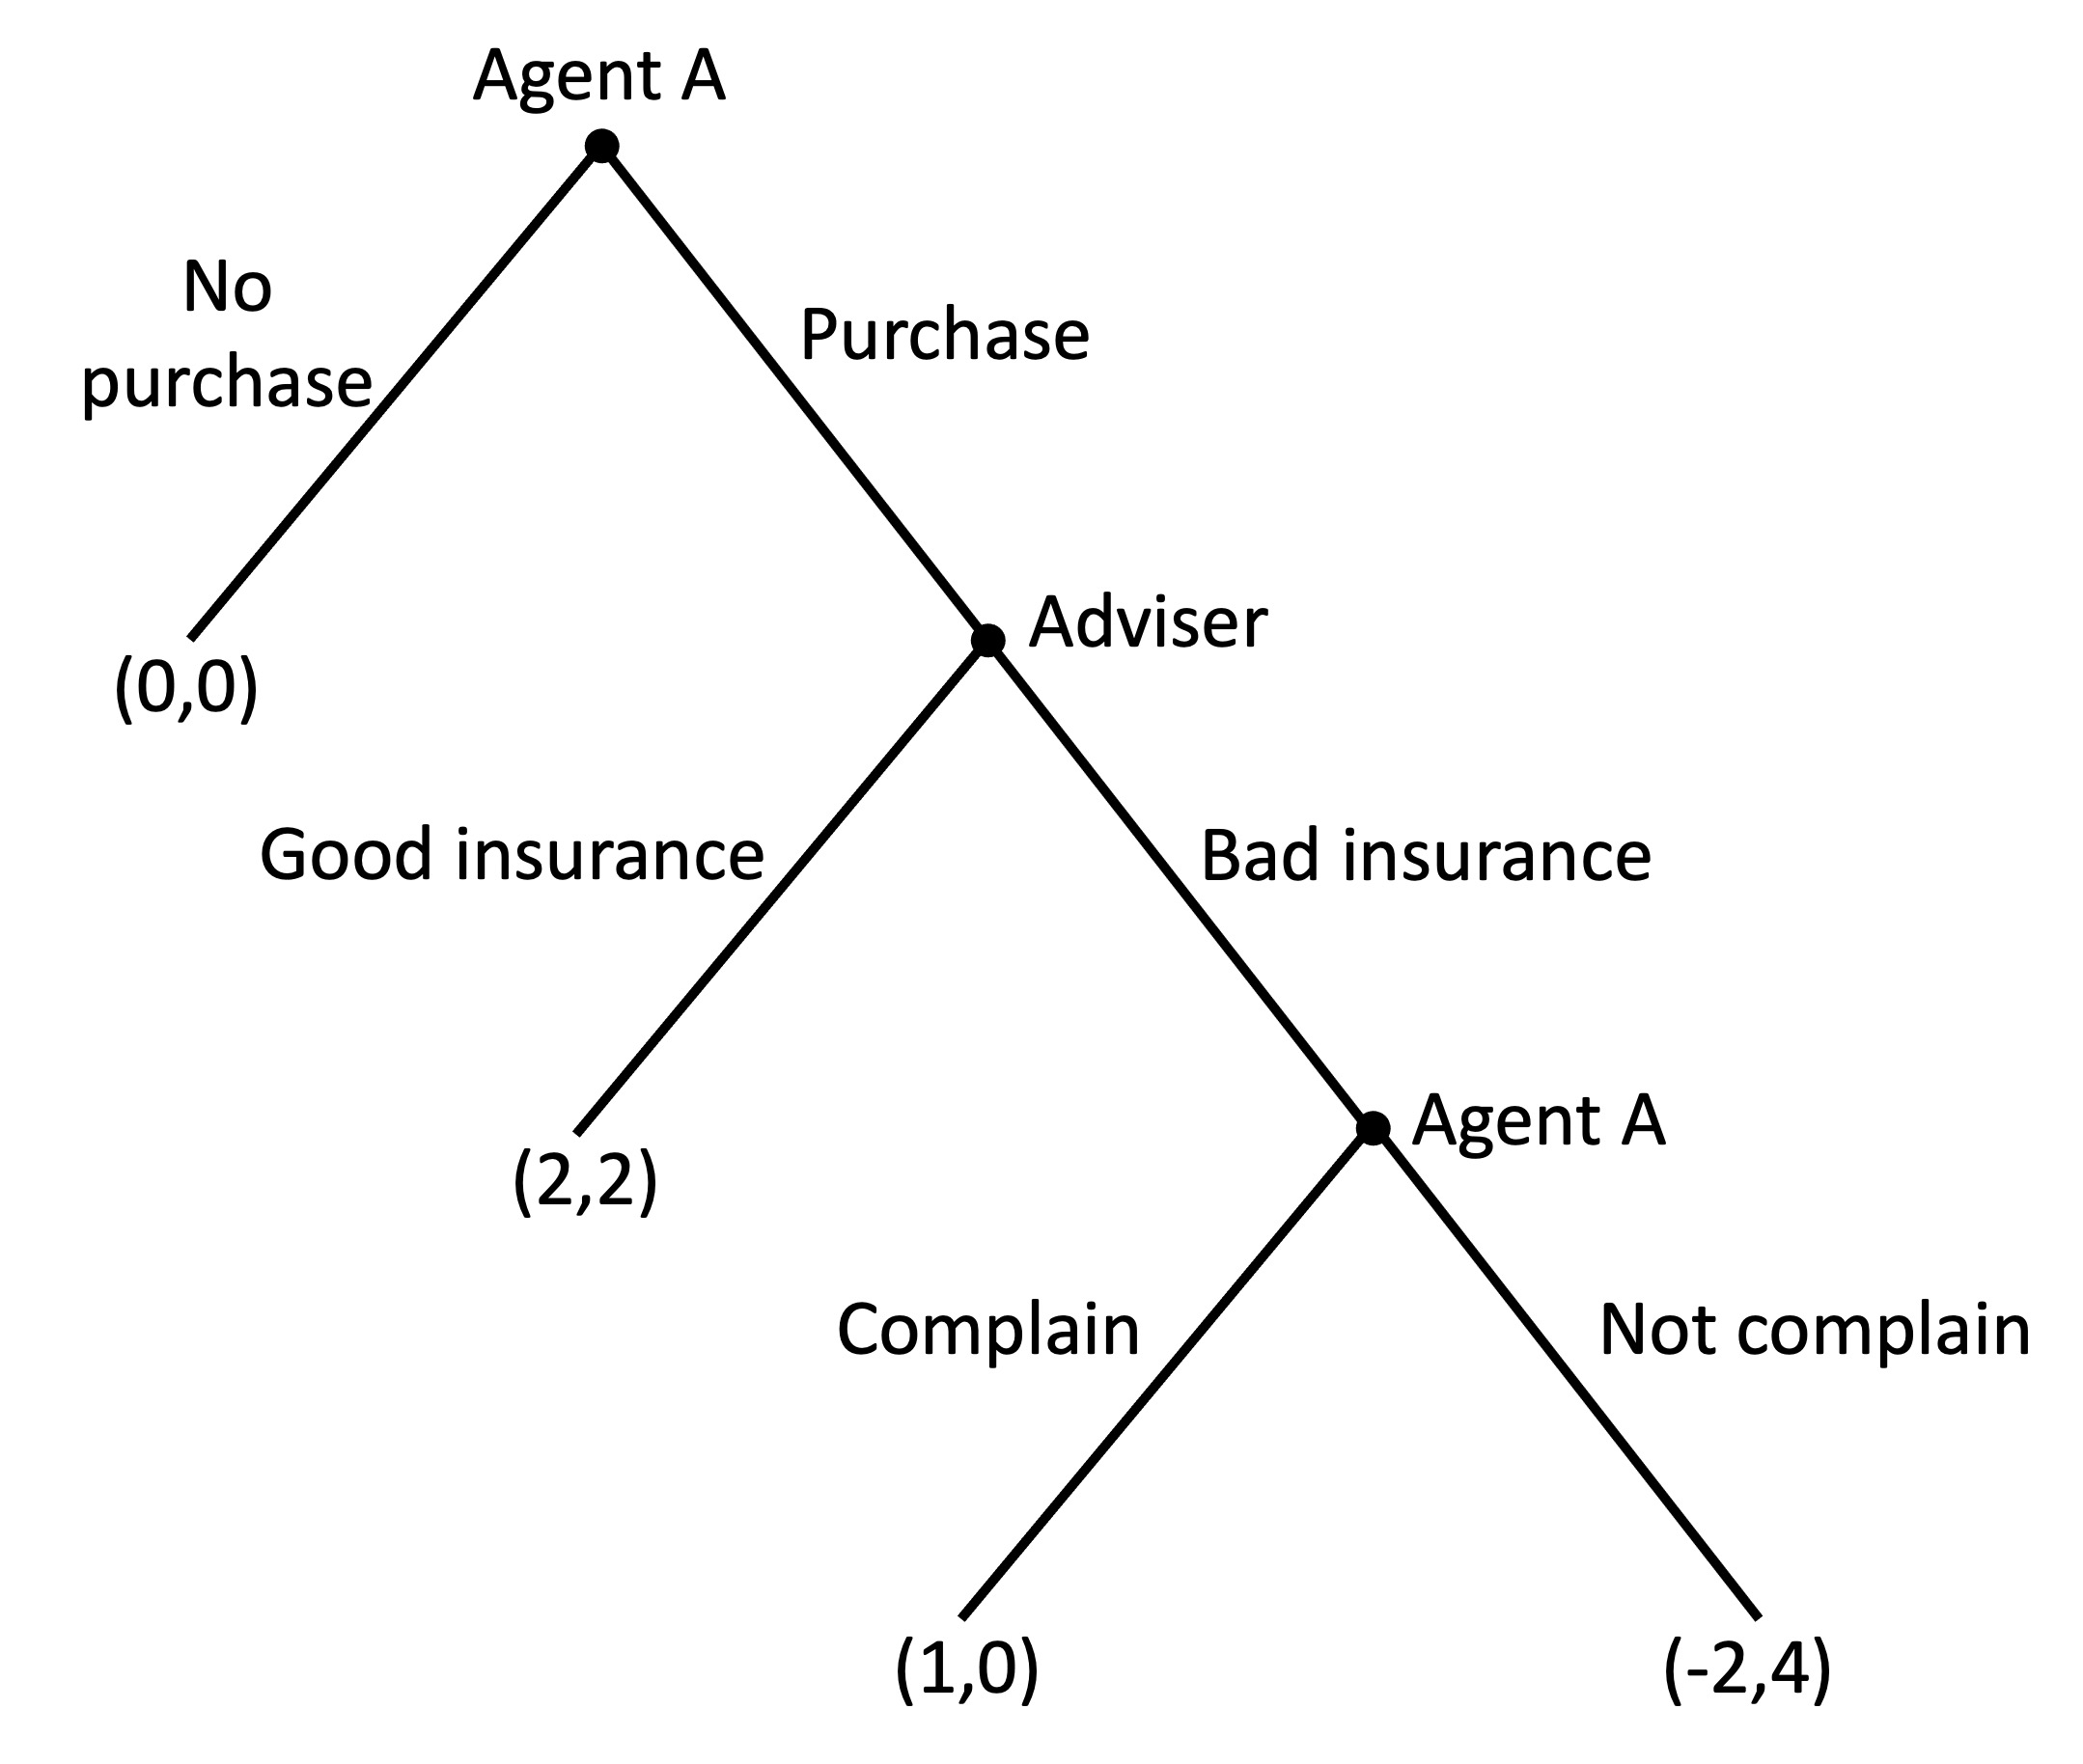
\includegraphics[width=0.6\textwidth,height=\textheight]{social-preferences/img/adviser-4.jpg}

The agent now has a choice between a payoff of 0 for selling bad
insurance (as Agent A complains and the insurance is cancelled) and 2
for selling good insurance. They sell the good insurance.

Agent A now has a choice of a payoff of 0 for not purchasing insurance
and 2 for purchasing. They make the purchase.

\hypertarget{social-preferences-exercises}{%
\chapter{Social preferences
exercises}\label{social-preferences-exercises}}

\hypertarget{fehr-schmidt-preferences}{%
\section{Fehr-Schmidt preferences}\label{fehr-schmidt-preferences}}

Alby has the following distributional preferences:

\[
U_A(x_A,x_j)=\underbrace{x_A}_{(1)}\underbrace{-\alpha\text{max}\{x_j-x_A,0\}}_{(2)}\underbrace{-\beta\text{max}\{x_A-x_j,0\}}_{(3)}
\]

where:

\(x_A\) is the outcome for Alby

\(x_j\) is the outcome for any agent \(j\) with whom Alby interacts.

a) For \(\alpha>0\) and \(\beta>0\), what are preferences of this form
are normally called?

\begin{tcolorbox}[enhanced jigsaw, title=\textcolor{quarto-callout-tip-color}{\faLightbulb}\hspace{0.5em}{Answer}, toprule=.15mm, colback=white, breakable, titlerule=0mm, colframe=quarto-callout-tip-color-frame, coltitle=black, opacityback=0, rightrule=.15mm, colbacktitle=quarto-callout-tip-color!10!white, bottomtitle=1mm, opacitybacktitle=0.6, arc=.35mm, bottomrule=.15mm, toptitle=1mm, leftrule=.75mm, left=2mm]

Inequality aversion.

\end{tcolorbox}

b) For \(\alpha>0\) and \(\beta>0\), describe the role of each of the
three terms labelled (1), (2) and (3) in the utility function.

\begin{tcolorbox}[enhanced jigsaw, title=\textcolor{quarto-callout-tip-color}{\faLightbulb}\hspace{0.5em}{Answer}, toprule=.15mm, colback=white, breakable, titlerule=0mm, colframe=quarto-callout-tip-color-frame, coltitle=black, opacityback=0, rightrule=.15mm, colbacktitle=quarto-callout-tip-color!10!white, bottomtitle=1mm, opacitybacktitle=0.6, arc=.35mm, bottomrule=.15mm, toptitle=1mm, leftrule=.75mm, left=2mm]

The first term captures the utility of Alby's own outcome.

The second term captures Alby's dislike of having less than others.

The third term captures Alby's dislike of having more than others.

\end{tcolorbox}

c) Explain the intuition for why we normally set \(\alpha>\beta\).

\begin{tcolorbox}[enhanced jigsaw, title=\textcolor{quarto-callout-tip-color}{\faLightbulb}\hspace{0.5em}{Answer}, toprule=.15mm, colback=white, breakable, titlerule=0mm, colframe=quarto-callout-tip-color-frame, coltitle=black, opacityback=0, rightrule=.15mm, colbacktitle=quarto-callout-tip-color!10!white, bottomtitle=1mm, opacitybacktitle=0.6, arc=.35mm, bottomrule=.15mm, toptitle=1mm, leftrule=.75mm, left=2mm]

Most people dislike having less than others more than they dislike
having more than others. In some instances, \(\beta<0\) in which case
people like having more than others - they are fine with inequality as
long as it is to their advantage.

\end{tcolorbox}

\hypertarget{charness-rabin-preferences}{%
\section{Charness-Rabin preferences}\label{charness-rabin-preferences}}

Bob has the following distributional preferences:

\[
u_B(x_B,x_j)=\left\{\begin{matrix}
\rho x_j+(1-\rho)x_B\quad &\textrm{if} \quad x_B \geq x_j \\[6pt]
\sigma x_j+(1-\sigma)x_B \quad &\textrm{if} \quad x_B < x_j 
\end{matrix}\right.
\]

where:

\(x_B\) is the outcome of the game for Bob

\(x_j\) is the outcome of the game for any agent \(j\) with whom Bob
interacts.

a) For \(1\geq \rho \geq\ 0 \geq \sigma\), what are preferences of this
form are normally called?

\begin{tcolorbox}[enhanced jigsaw, title=\textcolor{quarto-callout-tip-color}{\faLightbulb}\hspace{0.5em}{Answer}, toprule=.15mm, colback=white, breakable, titlerule=0mm, colframe=quarto-callout-tip-color-frame, coltitle=black, opacityback=0, rightrule=.15mm, colbacktitle=quarto-callout-tip-color!10!white, bottomtitle=1mm, opacitybacktitle=0.6, arc=.35mm, bottomrule=.15mm, toptitle=1mm, leftrule=.75mm, left=2mm]

Inequality aversion.

\end{tcolorbox}

b) For \(1\geq \rho \geq\ 0 \geq \sigma\), describe the role of the
terms in each of the two equations where \(x_B\geq x_j\) and
\(x_B< x_j\).

\begin{tcolorbox}[enhanced jigsaw, title=\textcolor{quarto-callout-tip-color}{\faLightbulb}\hspace{0.5em}{Answer}, toprule=.15mm, colback=white, breakable, titlerule=0mm, colframe=quarto-callout-tip-color-frame, coltitle=black, opacityback=0, rightrule=.15mm, colbacktitle=quarto-callout-tip-color!10!white, bottomtitle=1mm, opacitybacktitle=0.6, arc=.35mm, bottomrule=.15mm, toptitle=1mm, leftrule=.75mm, left=2mm]

\(\sigma\) and \(\rho\) are the weight that is Bob gives to the outcome
for agent \(j\). \(\sigma\) is applied where Bob's outcome is better
than or equal to that of agent \(j\), and \(\rho\) where it is worse.

The residual \(1-\sigma\) and \(1-\rho\) is the weight that Bob gives to
his own outcome.

\end{tcolorbox}

c) Explain the intuition why we normally set \(\rho>\sigma\) for the
utility function.

\begin{tcolorbox}[enhanced jigsaw, title=\textcolor{quarto-callout-tip-color}{\faLightbulb}\hspace{0.5em}{Answer}, toprule=.15mm, colback=white, breakable, titlerule=0mm, colframe=quarto-callout-tip-color-frame, coltitle=black, opacityback=0, rightrule=.15mm, colbacktitle=quarto-callout-tip-color!10!white, bottomtitle=1mm, opacitybacktitle=0.6, arc=.35mm, bottomrule=.15mm, toptitle=1mm, leftrule=.75mm, left=2mm]

People tend to be more willing to see others have better outcomes when
those others are worse off than them.

\end{tcolorbox}

d) What values of \(\rho\) and \(\sigma\) would result in a utility
function where Bob is purely self-interested?

\begin{tcolorbox}[enhanced jigsaw, title=\textcolor{quarto-callout-tip-color}{\faLightbulb}\hspace{0.5em}{Answer}, toprule=.15mm, colback=white, breakable, titlerule=0mm, colframe=quarto-callout-tip-color-frame, coltitle=black, opacityback=0, rightrule=.15mm, colbacktitle=quarto-callout-tip-color!10!white, bottomtitle=1mm, opacitybacktitle=0.6, arc=.35mm, bottomrule=.15mm, toptitle=1mm, leftrule=.75mm, left=2mm]

If Bob were purely self interested, \(\rho\) and \(\sigma\) would have a
value of zero. In that case, agent \(j\)'s outcomes would not enter into
the utility function. The utility function would become
\(u_B(x_B)=x_B\).

\end{tcolorbox}

e) What value must \(\sigma\) have to explain Bob's rejection of low
offers in the ultimatum game?

\begin{tcolorbox}[enhanced jigsaw, title=\textcolor{quarto-callout-tip-color}{\faLightbulb}\hspace{0.5em}{Answer}, toprule=.15mm, colback=white, breakable, titlerule=0mm, colframe=quarto-callout-tip-color-frame, coltitle=black, opacityback=0, rightrule=.15mm, colbacktitle=quarto-callout-tip-color!10!white, bottomtitle=1mm, opacitybacktitle=0.6, arc=.35mm, bottomrule=.15mm, toptitle=1mm, leftrule=.75mm, left=2mm]

Sigma must be negative such that the decrease in utility from agent
\(j\)'s payoff is larger than that through the payoff Bob receives
himself.

\end{tcolorbox}

f) Consider the following two scenarios involving the Ultimatum game.

Scenario 1: A proposer has a choice between offering a split of (\$8,
\$2) or (\$5, \$5). In experiments with this choice, responders tend to
reject offers of (\$8, \$2).

Scenario 2: A proposer has a choice between offering a split of (\$8,
\$2) or (\$10, \$0). In experiments with this choice, responders tend to
accept offers of (\$8, \$2).

A utility function of the type that Bob has cannot result in this
behaviour. Explain why.

\begin{tcolorbox}[enhanced jigsaw, title=\textcolor{quarto-callout-tip-color}{\faLightbulb}\hspace{0.5em}{Answer}, toprule=.15mm, colback=white, breakable, titlerule=0mm, colframe=quarto-callout-tip-color-frame, coltitle=black, opacityback=0, rightrule=.15mm, colbacktitle=quarto-callout-tip-color!10!white, bottomtitle=1mm, opacitybacktitle=0.6, arc=.35mm, bottomrule=.15mm, toptitle=1mm, leftrule=.75mm, left=2mm]

In both cases, the outcome is (\$8, \$2). This would result in the same
level of utility regardless of the other option that the proposer had.
If compared with the outcome (\$0, \$0) from rejecting the offer, the
action should therefore be the same.

An explanation for the difference between scenarios is that people care
not just about outcomes, but also the intentions of those with whom they
interact. In that circumstance the good (or otherwise) intentions of the
proposer in offering either less than they could or as much as they
could would shape the responder's action. However, intentions do not
enter into Bob's utility function.

\end{tcolorbox}

\bookmarksetup{startatroot}

\hypertarget{references}{%
\chapter*{References}\label{references}}
\addcontentsline{toc}{chapter}{References}

\markboth{References}{References}

\hypertarget{refs}{}
\begin{CSLReferences}{1}{0}
\leavevmode\vadjust pre{\hypertarget{ref-akerlof1970}{}}%
Akerlof, G. A. (1970). The market for {``}lemons{''}: Quality
uncertainty and the market mechanism*. \emph{The Quarterly Journal of
Economics}, \emph{84}(3), 488--500.
\url{https://doi.org/10.2307/1879431}

\leavevmode\vadjust pre{\hypertarget{ref-allais1953}{}}%
Allais, M. (1953). Le comportement de l'homme rationnel devant le
risque: Critique des postulats et axiomes de l'ecole americaine.
\emph{Econometrica}, \emph{21}(4), 503--546.
\url{https://doi.org/10.2307/1907921}

\leavevmode\vadjust pre{\hypertarget{ref-andreoni2009}{}}%
Andreoni, J., and Bernheim, B. D. (2009). Social Image and the
50{\textendash}50 Norm: A Theoretical and Experimental Analysis of
Audience Effects. \emph{Econometrica}, \emph{77}(5), 1607--1636.
\url{https://doi.org/10.3982/ECTA7384}

\leavevmode\vadjust pre{\hypertarget{ref-ashraf2006}{}}%
Ashraf, N., Karlan, D., and Yin, W. (2006). Tying odysseus to the mast:
Evidence from a commitment savings product in the philippines*.
\emph{The Quarterly Journal of Economics}, \emph{121}(2), 635--672.
\url{https://doi.org/10.1162/qjec.2006.121.2.635}

\leavevmode\vadjust pre{\hypertarget{ref-barber2001}{}}%
Barber, B. M., and Odean, T. (2001). Boys will be boys: Gender,
overconfidence, and common stock investment*. \emph{The Quarterly
Journal of Economics}, \emph{116}(1), 261--292.
\url{https://doi.org/10.1162/003355301556400}

\leavevmode\vadjust pre{\hypertarget{ref-barberis2006}{}}%
Barberis, N., Huang, M., and Thaler, R. H. (2006). Individual
Preferences, Monetary Gambles, and Stock Market Participation: A Case
for Narrow Framing. \emph{American Economic Review}, \emph{96}(4),
1069--1090. \url{https://doi.org/10.1257/aer.96.4.1069}

\leavevmode\vadjust pre{\hypertarget{ref-bar-eli2006}{}}%
Bar-Eli, M., Avugos, S., and Raab, M. (2006). Twenty years of {``}hot
hand{''} research: Review and critique. \emph{Psychology of Sport and
Exercise}, \emph{7}(6), 525--553.
\url{https://doi.org/10.1016/j.psychsport.2006.03.001}

\leavevmode\vadjust pre{\hypertarget{ref-camerer1999}{}}%
Camerer, C., and Lovallo, D. (1999). Overconfidence and Excess Entry: An
Experimental Approach. \emph{The American Economic Review},
\emph{89}(1), 13.

\leavevmode\vadjust pre{\hypertarget{ref-charness2002}{}}%
Charness, G., and Rabin, M. (2002). Understanding social preferences
with simple tests. \emph{The Quarterly Journal of Economics},
\emph{117}(3), 817--869. \url{https://www.jstor.org/stable/4132490}

\leavevmode\vadjust pre{\hypertarget{ref-cosmides1996}{}}%
Cosmides, L., and Tooby, J. (1996). Are humans good intuitive
statisticians after all? Rethinking some conclusions from the literature
on judgment under uncertainty. \emph{Cognition}, \emph{58}(1), 1--73.
\url{https://doi.org/10.1016/0010-0277(95)00664-8}

\leavevmode\vadjust pre{\hypertarget{ref-davidson1955}{}}%
Davidson, D., McKinsey, J. C. C., and Suppes, P. (1955). Outlines of a
Formal Theory of Value, I. \emph{Philosophy of Science}, \emph{22}(2),
140--160. \url{https://doi.org/10.1086/287412}

\leavevmode\vadjust pre{\hypertarget{ref-debondt1995}{}}%
De Bondt, W. F. M., and Thaler, R. H. (1995). \emph{Chapter 13 Financial
decision-making in markets and firms: A behavioral perspective} (Vol. 9,
pp. 385--410). Elsevier.
\url{https://doi.org/10.1016/S0927-0507(05)80057-X}

\leavevmode\vadjust pre{\hypertarget{ref-engel2011}{}}%
Engel, C. (2011). Dictator games: a meta study. \emph{Experimental
Economics}, \emph{14}(4), 583--610.
\url{https://doi.org/10.1007/s10683-011-9283-7}

\leavevmode\vadjust pre{\hypertarget{ref-eyster2005}{}}%
Eyster, E., and Rabin, M. (2005). Cursed Equilibrium.
\emph{Econometrica}, \emph{73}(5), 1623--1672.
\url{https://doi.org/10.1111/j.1468-0262.2005.00631.x}

\leavevmode\vadjust pre{\hypertarget{ref-farber2005}{}}%
Farber, H. S. (2005). Is tomorrow another day? The labor supply of new
york city cabdrivers. \emph{Journal of Political Economy},
\emph{113}(1), 46--82. \url{https://doi.org/10.1086/426040}

\leavevmode\vadjust pre{\hypertarget{ref-farber2008}{}}%
Farber, H. S. (2008). Reference-Dependent Preferences and Labor Supply:
The Case of New York City Taxi Drivers. \emph{American Economic Review},
\emph{98}(3), 1069--1082. \url{https://doi.org/10.1257/aer.98.3.1069}

\leavevmode\vadjust pre{\hypertarget{ref-farber2015}{}}%
Farber, H. S. (2015). Why you can{'}t find a taxi in the rain and other
labor supply lessons from cab drivers. \emph{The Quarterly Journal of
Economics}, \emph{130}(4), 1975--2026.
\url{https://doi.org/10.1093/qje/qjv026}

\leavevmode\vadjust pre{\hypertarget{ref-fehr1999}{}}%
Fehr, E., and Schmidt, K. M. (1999). A theory of fairness, competition,
and cooperation. \emph{The Quarterly Journal of Economics},
\emph{114}(3), 817--868. \url{https://www.jstor.org/stable/2586885}

\leavevmode\vadjust pre{\hypertarget{ref-frederick2002}{}}%
Frederick, S., Loewenstein, G., and O'Donoghue, T. (2002). Time
discounting and time preference: A critical review. \emph{Journal of
Economic Literature}, \emph{40}(2), 351--401.
\url{https://www.jstor.org/stable/2698382}

\leavevmode\vadjust pre{\hypertarget{ref-genesove2001}{}}%
Genesove, D., and Mayer, C. (2001). Loss aversion and seller behavior:
Evidence from the housing market. \emph{The Quarterly Journal of
Economics}, \emph{116}(4), 1233--1260.
\url{https://www.jstor.org/stable/2696458}

\leavevmode\vadjust pre{\hypertarget{ref-gigerenzer2011}{}}%
Gigerenzer, G. (2011). What are natural frequencies? \emph{BMJ},
\emph{343}, d6386. \url{https://doi.org/10.1136/bmj.d6386}

\leavevmode\vadjust pre{\hypertarget{ref-gigerenzer2021}{}}%
Gigerenzer, G. (2021). Embodied heuristics. \emph{Frontiers in
Psychology}, \emph{12}.
\url{https://www.frontiersin.org/articles/10.3389/fpsyg.2021.711289}

\leavevmode\vadjust pre{\hypertarget{ref-gilovich1985}{}}%
Gilovich, T., Vallone, R., and Tversky, A. (1985). The hot hand in
basketball: On the misperception of random sequences. \emph{Cognitive
Psychology}, \emph{17}(3), 295--314.
\url{https://doi.org/10.1016/0010-0285(85)90010-6}

\leavevmode\vadjust pre{\hypertarget{ref-ginuxe92010}{}}%
Giné, X., Karlan, D., and Zinman, J. (2010). Put Your Money Where Your
Butt Is: A Commitment Contract for Smoking Cessation. \emph{American
Economic Journal: Applied Economics}, \emph{2}(4), 213--235.
\url{https://doi.org/10.1257/app.2.4.213}

\leavevmode\vadjust pre{\hypertarget{ref-green1994}{}}%
Green, L., Fristoe, N., and Myerson, J. (1994). Temporal discounting and
preference reversals in choice between delayed outcomes.
\emph{Psychonomic Bulletin \& Review}, \emph{1}(3), 383--389.
\url{https://doi.org/10.3758/BF03213979}

\leavevmode\vadjust pre{\hypertarget{ref-heath1999}{}}%
Heath, C., Larrick, R. P., and Wu, G. (1999). Goals as Reference Points.
\emph{Cognitive Psychology}, \emph{38}(1), 79--109.
\url{https://doi.org/10.1006/cogp.1998.0708}

\leavevmode\vadjust pre{\hypertarget{ref-henrich2001}{}}%
Henrich, J., Boyd, R., Bowles, S., Camerer, C., Fehr, E., Gintis, H.,
and McElreath, R. (2001). In Search of Homo Economicus: Behavioral
Experiments in 15 Small-Scale Societies. \emph{American Economic
Review}, \emph{91}(2), 73--78. \url{https://doi.org/10.1257/aer.91.2.73}

\leavevmode\vadjust pre{\hypertarget{ref-hertwig1999}{}}%
Hertwig, R., and Gigerenzer, G. (1999). The {`}conjunction fallacy{'}
revisited: how intelligent inferences look like reasoning errors.
\emph{Journal of Behavioral Decision Making}, \emph{12}(4), 275--305.
\url{https://doi.org/10.1002/(SICI)1099-0771(199912)12:4\%3C275::AID-BDM323\%3E3.0.CO;2-M}

\leavevmode\vadjust pre{\hypertarget{ref-hoffrage1998}{}}%
Hoffrage, U., and Gigerenzer, G. (1998). Using natural frequencies to
improve diagnostic inferences. \emph{Academic Medicine}, \emph{73}(5),
53840. \url{https://doi.org/10.1097/00001888-199805000-00024}

\leavevmode\vadjust pre{\hypertarget{ref-hoffrage2015}{}}%
Hoffrage, U., Krauss, S., Martignon, L., and Gigerenzer, G. (2015).
Natural frequencies improve bayesian reasoning in simple and complex
inference tasks. \emph{Frontiers in Psychology}, \emph{6}, 1473.
\url{https://doi.org/10.3389/fpsyg.2015.01473}

\leavevmode\vadjust pre{\hypertarget{ref-johnson2003}{}}%
Johnson, E. J., and Goldstein, D. (2003). Do Defaults Save Lives?
\emph{Science}, \emph{302}(5649), 1338--1339.
\url{https://doi.org/10.1126/science.1091721}

\leavevmode\vadjust pre{\hypertarget{ref-johnson2011}{}}%
Johnson, N. D., and Mislin, A. A. (2011). Trust games: A meta-analysis.
\emph{Journal of Economic Psychology}, \emph{32}(5), 865--889.
\url{https://doi.org/10.1016/j.joep.2011.05.007}

\leavevmode\vadjust pre{\hypertarget{ref-kahneman2011}{}}%
Kahneman, D. (2011). \emph{Thinking, fast and slow} (1st edition).
Farrar, Straus; Giroux.

\leavevmode\vadjust pre{\hypertarget{ref-kahneman1991}{}}%
Kahneman, D., Knetsch, J. L., and Thaler, R. H. (1991). Anomalies: The
Endowment Effect, Loss Aversion, and Status Quo Bias. \emph{Journal of
Economic Perspectives}, \emph{5}(1), 193--206.
\url{https://doi.org/10.1257/jep.5.1.193}

\leavevmode\vadjust pre{\hypertarget{ref-kahneman1979}{}}%
Kahneman, D., and Tversky, A. (1979). Prospect theory: An analysis of
decision under risk. \emph{Econometrica}, \emph{47}(2), 263--291.
\url{https://doi.org/10.2307/1914185}

\leavevmode\vadjust pre{\hypertarget{ref-kahneman1984}{}}%
Kahneman, D., and Tversky, A. (1984). Choices, values, and frames.
\emph{American Psychologist}, \emph{39}(4), 341--350.
\url{https://doi.org/10.1037/0003-066X.39.4.341}

\leavevmode\vadjust pre{\hypertarget{ref-keynes1936}{}}%
Keynes, J. M. (1936). \emph{The general theory of employment, interest,
and money}. Macmillan.
\url{http://gutenberg.net.au/ebooks03/0300071h/printall.html}

\leavevmode\vadjust pre{\hypertarget{ref-kirby1995}{}}%
Kirby, K. N., and Herrnstein, R. J. (1995). Preference Reversals Due to
Myopic Discounting of Delayed Reward. \emph{Psychological Science},
\emph{6}(2), 83--89.
\url{https://doi.org/10.1111/j.1467-9280.1995.tb00311.x}

\leavevmode\vadjust pre{\hypertarget{ref-kirgios2020}{}}%
Kirgios, E. L., Mandel, G. H., Park, Y., Milkman, K. L., Gromet, D. M.,
Kay, J. S., and Duckworth, A. L. (2020). Teaching temptation bundling to
boost exercise: A field experiment. \emph{Organizational Behavior and
Human Decision Processes}, \emph{161}, 20--35.
\url{https://doi.org/10.1016/j.obhdp.2020.09.003}

\leavevmode\vadjust pre{\hypertarget{ref-koszegi2006}{}}%
Kőszegi, B., and Rabin, M. (2006). A model of reference-dependent
preferences. \emph{The Quarterly Journal of Economics}, \emph{121}(4),
1133--1165. \url{https://www.jstor.org/stable/25098823}

\leavevmode\vadjust pre{\hypertarget{ref-malmendier2005}{}}%
Malmendier, U., and Tate, G. (2005). CEO Overconfidence and Corporate
Investment. \emph{The Journal of Finance}, \emph{60}(6), 2661--2700.
\url{https://doi.org/10.1111/j.1540-6261.2005.00813.x}

\leavevmode\vadjust pre{\hypertarget{ref-martin2017}{}}%
Martin, V. (2017). When to quit: Narrow bracketing and reference
dependence in taxi drivers. \emph{Journal of Economic Behavior \&
Organization}, \emph{144}, 166--187.
\url{https://doi.org/10.1016/j.jebo.2017.09.024}

\leavevmode\vadjust pre{\hypertarget{ref-miller2018}{}}%
Miller, J. B., and Sanjurjo, A. (2018). Surprised by the Hot Hand
Fallacy? A Truth in the Law of Small Numbers. \emph{Econometrica},
\emph{86}(6), 2019--2047. \url{https://doi.org/10.3982/ECTA14943}

\leavevmode\vadjust pre{\hypertarget{ref-moore2007}{}}%
Moore, D. A., Oesch, J. M., and Zietsma, C. (2007). What Competition?
Myopic Self-Focus in Market-Entry Decisions. \emph{Organization
Science}, \emph{18}(3), 440--454.
\url{https://doi.org/10.1287/orsc.1060.0243}

\leavevmode\vadjust pre{\hypertarget{ref-moulin1986}{}}%
Moulin, H. (1986). \emph{Game theory for social sciences}. New York
Press.

\leavevmode\vadjust pre{\hypertarget{ref-nagel1995}{}}%
Nagel, R. (1995). Unraveling in guessing games: An experimental study.
\emph{The American Economic Review}, \emph{85}(5), 1313--1326.
\url{https://www.jstor.org/stable/2950991}

\leavevmode\vadjust pre{\hypertarget{ref-newton1990}{}}%
Newton, E. L. (1990). \emph{The rocky road from actions to intentions}
{[}PhD thesis{]}.
\url{https://www.proquest.com/openview/b740253d9b78599786f59d6b6055cc3b/1?pq-origsite=gscholar\&cbl=18750\&diss=y}

\leavevmode\vadjust pre{\hypertarget{ref-rabin2000}{}}%
Rabin, M. (2000). Risk Aversion and Expected-Utility Theory: A
Calibration Theorem. \emph{Econometrica}, \emph{68}(5), 1281--1292.
\url{http://www.jstor.org/stable/2999450}

\leavevmode\vadjust pre{\hypertarget{ref-rabin2002}{}}%
Rabin, M. (2002). Inference by believers in the law of small numbers.
\emph{The Quarterly Journal of Economics}, \emph{117}(3), 775--816.
\url{https://doi.org/10.1162/003355302760193896}

\leavevmode\vadjust pre{\hypertarget{ref-rabin2010}{}}%
Rabin, M., and Vayanos, D. (2010). The gambler's and hot-hand fallacies:
Theory and applications. \emph{The Review of Economic Studies},
\emph{77}(2), 730--778.
\url{https://doi.org/10.1111/j.1467-937X.2009.00582.x}

\leavevmode\vadjust pre{\hypertarget{ref-rapoport1997}{}}%
Rapoport, A., and Budescu, D. V. (1997). Randomization in individual
choice behavior. \emph{Psychological Review}, \emph{104}, 603--617.
\url{https://doi.org/10.1037/0033-295X.104.3.603}

\leavevmode\vadjust pre{\hypertarget{ref-read1998}{}}%
Read, D., and Leeuwen, B. van. (1998). Predicting Hunger: The Effects of
Appetite and Delay on Choice. \emph{Organizational Behavior and Human
Decision Processes}, \emph{76}(2), 189--205.
\url{https://doi.org/10.1006/obhd.1998.2803}

\leavevmode\vadjust pre{\hypertarget{ref-shefrin1985}{}}%
Shefrin, H., and Statman, M. (1985). The Disposition to Sell Winners Too
Early and Ride Losers Too Long: Theory and Evidence. \emph{The Journal
of Finance}, \emph{40}(3), 777--790.
\url{https://doi.org/10.1111/j.1540-6261.1985.tb05002.x}

\leavevmode\vadjust pre{\hypertarget{ref-spiegelhalter2015}{}}%
Spiegelhalter, D., and Gage, J. (2015). What can education learn from
real-world communication of risk and uncertainty? \emph{The Mathematics
Enthusiast}, \emph{12}(1), 4--10.
\url{https://doi.org/10.54870/1551-3440.1329}

\leavevmode\vadjust pre{\hypertarget{ref-thaler1981}{}}%
Thaler, R. (1981). Some empirical evidence on dynamic inconsistency.
\emph{Economics Letters}, \emph{8}(3), 201--207.
\url{https://doi.org/10.1016/0165-1765(81)90067-7}

\leavevmode\vadjust pre{\hypertarget{ref-thaler1980}{}}%
Thaler, R. (1980). Toward a positive theory of consumer choice.
\emph{Journal of Economic Behavior \& Organization}, \emph{1}(1),
39--60. \url{https://doi.org/10.1016/0167-2681(80)90051-7}

\leavevmode\vadjust pre{\hypertarget{ref-thaler2004}{}}%
Thaler, Richard~H., and Benartzi, S. (2004). Save More
Tomorrow{\texttrademark}: Using Behavioral Economics to Increase
Employee Saving. \emph{Journal of Political Economy}, \emph{112}(S1),
S164--S187. \url{https://doi.org/10.1086/380085}

\leavevmode\vadjust pre{\hypertarget{ref-tversky1974}{}}%
Tversky, A., and Kahneman, D. (1974). Judgment under Uncertainty:
Heuristics and Biases. \emph{Science}, \emph{185}(4157), 1124--1131.
\url{https://doi.org/10.1126/science.185.4157.1124}

\leavevmode\vadjust pre{\hypertarget{ref-tversky1982}{}}%
Tversky, A., and Kahneman, D. (1982). \emph{Evidential impact of base
rates} (A. Tversky, D. Kahneman, and P. Slovic, Eds.; pp. 153--160).
Cambridge University Press.
\url{https://doi.org/10.1017/CBO9780511809477.011}

\leavevmode\vadjust pre{\hypertarget{ref-tversky1983}{}}%
Tversky, A., and Kahneman, D. (1983). Extensional versus intuitive
reasoning: The conjunction fallacy in probability judgment.
\emph{Psychological Review}, \emph{90}(4), 293--315.
\url{https://doi.org/10.1037/0033-295X.90.4.293}

\leavevmode\vadjust pre{\hypertarget{ref-zelmer2003}{}}%
Zelmer, J. (2003). Linear Public Goods Experiments: A Meta-Analysis.
\emph{Experimental Economics}, \emph{6}(3), 299--310.
\url{https://doi.org/10.1023/A:1026277420119}

\end{CSLReferences}



\end{document}
